\documentclass[12pt, twoside]{book}

% Package Imports
\usepackage[a4paper, margin=2.5cm]{geometry}
\usepackage{amsmath, amssymb, amsthm, amstext, amsfonts}
\usepackage[mathscr]{eucal}
\usepackage{graphicx}
\usepackage{array, tabularx, longtable}
\usepackage{multicol}
\usepackage{makeidx}
\usepackage{indentfirst}
\usepackage[utf8]{inputenc}
\usepackage[utf8]{vietnam} % Necessary for Vietnamese text
\usepackage{hyperref}
\usepackage{wrapfig}
\usepackage{chngpage}
\usepackage{fancybox}
\usepackage{color}
\usepackage{pagecolor}
\usepackage{wallpaper, mdframed}
\usepackage{tcolorbox}
\usepackage{adjustbox}
\usepackage{epigraph}
\usepackage{subcaption}
\usepackage{capt-of}
\usepackage{perpage} 
\MakePerPage{footnote}
\usepackage{fancyhdr}
\usepackage{titlesec}
\usepackage{lipsum}

% Font and Color Definitions
\definecolor{C1}{rgb}{0,0.2,0.5}
\definecolor{C2}{rgb}{0.6,0,0.2}
\definecolor{C3}{rgb}{0.2,0.4,0.6}

% Header and Footer
\pagestyle{fancy}
\fancyhf{}
\fancyhead[LE,RO]{\thepage}
\renewcommand{\headrulewidth}{0pt} % No line in header area

% Customizing the table of contents
\makeatletter
\renewcommand{\l@chapter}{\@dottedtocline{1}{0.5cm}{0.8cm}}
\renewcommand{\l@section}{\@dottedtocline{2}{0.7cm}{0.8cm}}
\makeatother

% Title Page
\begin{document}
\thispagestyle{empty}
\vspace*{0.1cm}
\centerline{\textcolor{C2}{\bf {\LARGE PHAN ĐÌNH DIỆU}}} 
\vspace*{1cm}
\centerline{\textcolor{C1}{\fontsize{32}{45}\selectfont \textit{\textbf{NGHĨ SUY}}}}
\centerline{\textcolor{C1}{\fontsize{32}{45}\selectfont \textit{\textbf{CÙNG ĐẤT NƯỚC}}}}
\vspace{1cm}
\centerline{\textcolor{C2}{\large \bf Sưu tầm và tuyển chọn}}
\vspace{1.5cm}
\vfill
\centerline{\textcolor{C1}{\large Tủ sách Sputnik, số XX001}}
\vspace{1cm}
\centerline{\textcolor{C2}{\Large Nhà xuất bản Thế Giới}}
\newpage

% Information Page
\textbf{\Large Nghĩ Suy Cùng Đất Nước} 

\textit{Sưu tầm và tuyển chọn}.

\textit{Tác giả}: \textbf{Phan Đình Diệu}

\textit{Tranh bìa}: \textbf{Lã Đạt}

\textit{Các tranh minh họa bên trong}: chuyển từ ảnh sưu tầm. 

\vspace{0.3cm}

\textit{Cuốn sách này giới thiệu một số bài viết, phát biểu thẳng thắn và tâm huyết của ông Phan Đình Diệu nhằm đóng góp vào việc phát triển đất nước. Đó là những ý kiến công khai trên diễn đàn Quốc hội, diễn đàn Mặt trận Tổ quốc hay những kiến nghị gửi lãnh đạo nhà nước và những bài trả lời phỏng vấn với báo chí nước ngoài tại Việt nam. Hy vọng bạn đọc có thêm tư liệu về một giai đoạn lịch sử thông qua những suy nghĩ, trăn trở của một người trí thức, của một người công dân với tinh thần như ông đã phát biểu trong bài « Góp Ý Kiến về Đổi Mới » tháng 9/1986: « Tôi hi vọng rằng, những ý kiến trên đây sẽ được xem là phần đóng góp giọt nước nhỏ bé của mình vào hơn 60 triệu giọt nước khác của dân tộc để hoà thành dòng thác đổi mới của đất nước ta hiện nay ».}

\newpage

% Table of Contents
\tableofcontents

% Chapter 1
\chapter*{Điếu văn truy điệu Giáo sư Phan Đình Diệu}
\addcontentsline{toc}{chapter}{Điếu văn truy điệu Giáo sư Phan Đình Diệu}
%\input{chapter1.tex} % Assuming content for chapters is stored in separate .tex files


% Other chapters
% Add more chapters here as necessary

%\end{document}

% \newpage
% \begin{center}
% {\bf Điếu văn truy điệu Giáo sư Phan Đình Diệu}
% \end{center}

Kính thưa quý vị thân hữu, bạn bè, đồng nghiệp,

Thưa gia quyến Thầy Phan Đình Diệu, 

Hôm nay chúng ta cùng nhau ở đây để tiễn đưa Giáo sư Phan Đình Diệu – một nhà khoa học - một nhà giáo - một trí thức lớn của Việt Nam – người đã đặt nền móng cho sự hình thành và phát triển ngành khoa học tính toán và tin học Việt Nam, người có sức ảnh hưởng lớn đến xã hội qua những đóng góp tâm huyết với tầm nhìn xa rộng cho sự phát triển đất nước. 
Sinh năm 1936 tại xã Trung Lộc, huyện Can Lộc, tỉnh Hà Tĩnh trong một gia đình có truyền thống hiếu thuận và hiếu học, ngay từ nhỏ cậu bé Phan Đình Diệu đã bộc lộ một tư chất thông minh đĩnh ngộ. Mới 4 tuổi, cậu đã được thầy giáo cõng đi học cùng các anh chị lớn, và ngay khi 9 tuổi đã được thay mặt thiếu nhi diễn thuyết trước cả hội trường lớn vào những ngày tháng 8 năm 1945 lịch sử. Cha cậu là thầy giáo thường đi dạy xa nhà, mẹ làm nông tần tảo nuôi 7 anh em, là con trưởng nên ngay từ nhỏ, Phan Đình Diệu đã có ý thức tự lập và trách nhiệm, luôn có tấm lòng giúp đỡ và dìu dắt những lớp đàn em đi sau mình. 

Những năm tháng học ở trường cấp III Phan Đình Phùng, nay là trường Trung học phổ thông Phan Đình Phùng, Thành phố Hà Tĩnh, Giáo sư Phan Đình Diệu đã có những người bạn tâm giao, những người sau này trở thành những nhà khoa học trong nhiều lĩnh vực. Ngôi trường ấy cũng cho ông ký ức đẹp về những người thầy mà ông đã thể hiện sự kính yêu qua những bài viết có sức lay động sâu sắc. 

Năm 1954, ông ra Hà Nội và theo học Trường Đại học Sư Phạm Hà Nội. Trong thời gian này, ngoài việc miệt mài học tập, ông cũng đã tự học tiếng Anh và tiếng Pháp, và rất say mê tìm hiểu về Triết học. Chính ở đây ông đã tìm thấy niềm đam mê với Toán học, đã tốt nghiệp thủ khoa xuất sắc. Ngay sau đó, ông được giữ lại trường làm giảng viên và giảng dạy tại đây từ năm 1957 đến 1962.

Năm 1962 ông được cử sang Liên xô làm Nghiên cứu sinh. Năm 1965, với những kết quả xuất sắc khi bảo vệ luận án Phó Tiến sĩ, Ông đã được Hội đồng đề xuất để thực hiện tiếp luận án Tiến sĩ khoa học. 

Năm 1967, ông đã bảo vệ thành công luận án Tiến sĩ khoa học khi ở tuổi 30. Các công trình khoa học có tính đột phá trong giai đoạn này của ông đã được xuất bản trên các tạp chí hàng đầu của Nga, góp phần mở một nhánh mới trong Toán học về Giải tích hàm kiến thiết và được in riêng thành một tập của tạp chí khoa học Steklov của Nga. Năm 1974, được Hiệp hội Toán học Mỹ dịch và xuất bản thành cuốn sách bằng tiếng Anh.

Sau khi về nước, Tiến sĩ khoa học trẻ Phan Đình Diệu làm việc ở Uỷ ban khoa học kỹ thuật nhà nước, tham gia vào Phòng Toán học tính toán và đồng thời kiêm nhiệm tổ trưởng bộ môn Điều khiển học, một trong bốn bộ môn của Viện Toán học trong những ngày đầu thành lập. 

Ngay từ đầu những năm 1970, nhận định về tình hình thế giới, cho rằng thông tin, tri thức sẽ ngày càng đóng vai trò quan trọng và coi đây là cuộc cách mạng lớn thay đổi nhân loại, ông cùng đồng nghiệp đề xuất dự án thành lập Viện Khoa học Tính toán và Điều khiển. 

Năm 1977, Viện Khoa học Tính toán và Điều khiển chính thức được thành lập, và ông là Viện trưởng đầu tiên. Viện là tiền thân của Viện Tin học, sau đổi tên là Viện CNTT hiện nay. 

Giáo sư Phan Đình Diệu đã luôn phát hiện, khuyến khích những cán bộ nghiên cứu trẻ có năng lực, xây dựng các những nhóm nghiên cứu mạnh. Dưới sự lãnh đạo tâm huyết và quyết đoán của ông và với sự quyết tâm và làm việc hăng say các cán bộ của Viện, năm 1979, chiếc máy vi tinh đầu tiên được thiết kế và sản xuất tại Việt Nam và Đông Nam Á. Ông cũng đã lãnh đạo nhóm nghiên cứu hợp tác với Bộ Nội Vụ và Ban Cơ yếu Chính phủ để phát triển các thiết bị tự động giải mật và mật mã hoá. Năm 2007, các nghiên cứu này đã được trao tặng giải thưởng Nhà nước về KH\&CN.

Giáo sư Phan Đình Diệu đã tích cực xây dựng nhiều hợp tác khoa học với quốc tế. Ông đã được mời đến giảng bài hoặc làm Giáo sư mời nhiều trường đại học uy tín trên thế giới ở Pháp, Mỹ, Đức, Nga, Canada, Tây Ban Nha, Nhật Bản, Hungary, Bugary, Ba Lan, Phần Lan. Với ảnh hưởng và uy tín của mình, Ông đã tổ chức thành công các Hội nghị Tin học quốc tế đầu tiên ở Việt Nam, và mời được các chuyên gia Tin học nước ngoài về nước để phát triển các nhóm nghiên cứu trong nước. 

Cùng với sự phát triển của đội ngũ cán bộ KH\&CN trong cả nước, ông đã sáng lập ra Hội Tin học Việt Nam vào cuối năm 1988 và đảm nhận trách nhiệm Chủ tịch Hội hai khoá đầu tiên. 

Vào đầu những năm 1990, ông đã dồn tâm huyết để thực hiện nhiệm vụ được Nhà nước giao biên soạn ``Chính sách phát triển và ứng dụng CNTT'' làm nền tảng cho sự ra đời của Chương trình quốc gia về CNTT. 

Năm 1993, Ông được chỉ định làm Phó trưởng Ban thường trực Ban chỉ đạo Chương trình quốc gia về CNTT và là người trực tiếp soạn thảo Chương trình Quốc gia về CNTT giai đoạn 1995-2000, đặt nền tảng cho việc ứng dụng CNTT vào mọi mặt kinh tế xã hội, như xây dựng chính phủ điện tử, đưa Internet vào Việt Nam, xây dựng các Khoa CNTT trọng điểm và mở các chương trình đào tạo tại các trường đại học.

Dù ở bất cứ cương vị công tác nào, Viện trưởng Viện Tính toán và Điều khiển, Viện phó Viện Khoa học Việt Nam, Chủ tịch Hội đồng chức danh Giáo sư ngành Toán, Trưởng ban xét duyệt và hỗ trợ của Quỹ VIFOTEC của Liên hiệp các Hội KHKT Việt Nam hay Chủ tịch Hội đồng tư vấn về Tin học của Liên hiệp Hội, Giáo sư Phan Đình Diệu luôn thể hiện tinh thần trách nhiệm và sự tâm huyết với công việc.

Ở tuổi lục tuần, Giáo sư Phan Đình Diệu lại trở về giảng dạy tại Trường Đại học Công Nghệ - Đại học Quốc gia Hà Nội.

Trong suốt sự nghiệp dạy học, ông đã dạy nhiều môn học, biên soạn nhiều giáo trình, đặc biệt là các môn học có tính chất khai mở, dự báo những hướng đi mới của sự phát triển khoa học tính toán, như các sách về Logic toán - cơ sở toán học của tin học, Lý thuyết độ phức tạp tính toán, Lý thuyết mật mã và an toàn thông tin. Những bài viết khoa học, những cuốn sách và giáo trình đều được ông viết rất trong sáng, sâu sắc, chặt chẽ và đầy tính sư phạm.

Không chỉ là một nhà khoa học, một giảng viên, suốt cả cuộc đời Giáo sư Phan Đình Diệu còn là một người trí thức đóng góp trí tuệ và tâm huyết cho đất nước. 

Là Đại biểu Quốc hội khoá 5 và khoá 6, tham gia Uỷ viên của Uỷ ban Đối ngoại, rồi Uỷ ban Văn hoá và Giáo dục của Quốc hội, với tư duy độc lập, logic, kết hợp với sự tìm hiểu sâu sắc về triết học và chính trị xã hội, Giáo sư Phan Đình Diệu đã có những cách nhìn sâu rộng về thời cuộc, về xu hướng phát triển và những sự đổi thay cần thiết cho đất nước. Các ý tưởng của ông luôn được hình thành trên cơ sở khoa học, các dữ liệu thực tế và các vấn đề cốt lõi của sự phát triển kinh tế - xã hội; luôn có sự nhất quán, xuyên suốt, mang một tầm nhìn xa, có giá trị qua nhiều thập kỷ. 

Ở mọi diễn đàn trong nước hay quốc tế, ngay cả trên diễn đàn Quốc hội, Mặt trận Tổ Quốc, trước lãnh đạo cấp cao, Phan Đình Diệu luôn thể hiện là một trí thức thẳng thắn, chân thành và tâm huyết vì sự phát triển của đất nước.

Trong xã hội, vốn là người sâu lắng, nhưng tâm hồn chất chứa nét phóng khoáng nghệ sĩ và một tầm hiểu biết xã hội rộng mở, ông có rất nhiều bạn bè tâm giao. Ngôi nhà của vợ chồng ông không chỉ là nơi những bạn bè, đồng nghiệp, học trò trao đổi về học thuật, nơi nhiều trí thức tranh luận về xã hội và đất nước, mà còn là nơi bao bạn bè nghệ sĩ cùng thưởng thức nhiều bản nhạc câu thơ.

Là người con của vùng đất Hà Tĩnh, một nhà khoa học, một giảng viên, một trí thức có nhiều đóng góp với sự phát triển của KH\&CN nước nhà, Giáo sư Phan Đình Diệu luôn trăn trở và giúp đỡ quê hương. Ông là một con người luôn có trách nhiệm và là trụ cột của gia đình, dòng tộc. Là con trưởng, ông trọn lòng hiếu thảo với cha mẹ, chăm lo và dìu dắt sáu người em. Trong gia đình, Giáo sư Phan Đình Diệu là người chồng thuỷ chung, hết mực yêu thương vợ con.

Noi theo tấm gương khoa học trung thực, luôn nhìn thẳng và nói thẳng của đấng sinh thành, cả ba người con ông đều trưởng thành trong sự nghiệp và hiếu thuận với mẹ cha. 

{\em Kính thưa quí vị ! Kính thưa quí quyến !}

Giáo sư Phan Đình Diệu ra đi để lại một khoảng trống cho gia đình, họ tộc, cho quê hương đất nước. Giáo sư đã đi xa nhưng cuộc đời, sự nghiệp, đức độ, thanh danh của Giáo sư mãi còn trong nỗi tiếc thương vô hạn của gia đình, của bạn bè, họ hàng gần xa và của tất cả những ai dù chỉ biết ông qua các trang sách, bài báo. 

Thay mặt Ban tang lễ, xin kính cẩn vĩnh biệt Giáo sư. Xin cầu nguyện cho Giáo sư siêu sinh tính độ. Xin chân thành và thống thiết chia buồn cùng bà quả phụ, các con, các cháu nội ngoại và họ tộc của Giáo sư.

Sau đây, xin tất cả dành một phút mặc niệm Giáo sư Phan Đình Diệu !
(Giáo sư Nguyễn Hữu Đức, phó Giám đốc Đại học Quốc gia Hà Nội đọc. 18-5-2018)
\newpage 

% Chapter 2
\chapter*{Lời cảm ơn và Lời với bố}
\addcontentsline{toc}{chapter}{Lời cảm ơn và Lời với bố}
%\input{chapter2.tex}


% \begin{center}
% {\bf Lời cảm ơn và Lời với bố.}
% \end{center}

Kính thưa Ban tổ chức lễ tang.

Kính thưa các cụ, các ông các bà, các bác các cô các chú, anh chị em bạn bè hàng xóm láng giềng gần xa và thân bằng cố hữu của bố chúng tôi.

Kính thưa các quý vị, đại diện các cơ quan đoàn thể.

Từ khi bố chúng tôi lâm bệnh đến tận những phút giây cuối cùng và trong cả buổi tang lễ hôm nay, chúng tôi đã nhận được rất nhiều sự chia sẻ, giúp đỡ của các y bác sỹ, của bạn bè và người thân.

Chúng tôi không biết nói gì hơn là lòng cảm ơn chân thành của cả gia đình tới các ông bà, chú bác, anh chị em và các quý vị, bạn bè của gia đình.

Trong những ngày bố tôi ốm nặng, ông đã được sự quan tâm đặc biệt của tập thể các bác sỹ, y tá, điều dưỡng viên của khoa hồi sức cấp cứu bệnh viện 354 và khoa cấp cứu A9 bệnh viện Bạch Mai. Chúng tôi sẽ không thể nào quên tấm lòng của các y bác sỹ đã hết lòng cứu chữa cho bố tôi.

Chúng tôi cũng xin cảm ơn các cô chú, bạn bè đã gửi những lời động viên sâu sắc trên báo chí, trên mạng xã hội, qua thư điện tử những hồi ức và kỷ niệm về bố.

Chúng tôi chân thành cảm ơn ĐHQG Hà nội, Đại học công nghệ, Viện Hàn lâm khoa học Việt nam, Viện CNTT và các đơn vị trong ban tổ chức tang lễ, nhà tang lễ bệnh Viện trung ương quân đội 108, đã tận tình giúp đỡ gia đình tổ chức tang lễ được chu toàn.
%\newpage 

\paragraph{Lời với bố. }
Sau đây tôi xin được nói đôi lời với bố.

Thưa bố,

Lời nói thiêng liêng nhất con xin cảm ơn bố, cuộc đời bố đã để lại cho mẹ, cho chúng con một tinh thần đầy yêu thương và chính trực.

Bố luôn thẳng thắn nhưng cũng rất hài hước và lãng mạn. Mẹ kể, lần gặp đầu tiên, bố tặng mẹ cuốn truyện Ruồi Trâu với một ánh mắt long lanh. Bố làm những bài thơ tặng mẹ đến ông ngoại cũng mê và chép lại. Mỗi niềm vui trăn trở trong công việc, mỗi bài viết tâm huyết với đất nước bố đều chia sẻ với mẹ. Tình yêu của bố sẽ giúp mẹ luôn vững vàng, như sự mạnh mẽ lạc quan mẹ đã luôn có trong những năm qua, khi chăm sóc sức khoẻ cho bố.

Đối với chúng con, niềm say mê của bố đối với khoa học, những trăn trở của bố đối với đất nước, là lời dạy vô giá. Bố nói với con, cuộc sống cần nhất sự trung thực. Tưởng chừng đơn giản nhưng trung thực bao gồm cả dũng cảm, trung thực với chính mình để có những chính kiến độc lập, và trung thực trong cuộc đời để dũng cảm nói lên những ý kiến tâm huyết.

Những lời phát biểu chân thành của bố thật dũng cảm, giản dị nhưng đầy mạnh mẽ về đất nước - như mong ước của bố - những ý kiến của mình sẽ như một giọt nước nhỏ bé hoà vào nhiều triệu giọt nước khác của dân tộc để tạo thành dòng thác “đổi mới" của đất nước.

Giọt nước nhỏ bé đó, như bố lấy tên, là những bài viết « Nghĩ suy cùng đất nước ». Giọt nước đó sẽ không tan đi khi bố chia xa.

Câu thơ bố viết cho con khi con còn nhỏ từ đất nước Đan Mạch của An-đéc-sen sẽ mãi đồng hành cùng con :\\
{\em 
« Và con ơi,\\
Bố muốn tặng con\\
một chú ngựa rơm\\
Trên gập ghềnh đường xa\\ 
con sẽ bước »\\
}

Một lần nữa, xin gửi lời cảm ơn đến tất cả các ông bà, chú bác, anh chị em và các quý vị, bạn bè của gia đình đã đến dự lễ viếng và đã gửi vòng hoa cũng như giúp đỡ chúng tôi tổ chức buổi tiễn đưa bố tôi ngày hôm nay. Trong lúc tang gia bối rối, không tránh khỏi sơ xuất, chúng tôi rất mong có sự thông cảm và lượng thứ.

Phan Dương Hiệu.




$\copyright$ Phan Đình Diệu - Phan Dương Hiệu và Sputnik Education, 2018.

\newpage
\begin{figure}
\centering
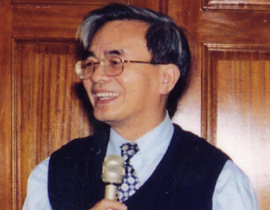
\includegraphics[scale=1]{phandinhdieu1}
\caption{Giáo sư Phan Đình Diệu}
\end{figure}

\newpage


%\fancyhead{}
%\thispagestyle{plain}
\begin{scriptsize}
%\textcolor{C1}{
\tableofcontents 
%}
\end{scriptsize}


\part{Nghĩ Suy Cùng Đất Nước}
\clearpage{\pagestyle{empty}\cleardoublepage}


\chapter{Tham luận tại Quốc Hội 12/1978: Đưa khoa học kỹ thuật phục vụ tích cực và có hiệu quả hơn công tác cải tiến quản lý}
\begin{center}
Tham luận của đồng chí PHAN – ĐÌNH – DIỆU\\
 đại biểu Thái – bình.
\end{center}
\textit{Kính thưa Đoàn chủ tịch,\\
Kính thưa các đồng chí đại biểu Quốc hội,}


 Cải tiến quản lý kinh tế là một vấn đề cấp bách mà tất cả chúng ta đều quan tâm. Những hiện tượng khuyết điểm trong công tác tổ chức quản lý và chỉ đạo thực hiện là điều mà hầu như mọi người đều thấy. Tuy nhiên, phân tích thực chất của những khuyết điểm đó, hiểu rõ những đặc điểm bản chất của công tác quản lý trong thười đại ngày nay để từ đó tìm ra được các biện pháp cải tiến có hiệu quả thì lại là một việc hết sức phức tạp và khó khăn. Dưới đây, với nhận thức của một cán bộ khoa học kỹ thuật, chúng tôi xin mạnh dạn góp một vài ý kiến nhỏ.
 
 
 Chúng tôi hoàn toàn đồng ý với những phân tích các khuyết điểm được nêu trong báo cáo của Chính phủ về các mặt vận dụng các quy luật kinh tế của chủ nghĩa xã hội, về công tác kế hoạch hóa, và về tổ chức quản lý và chỉ đạo thực hiện.
 
 
 Vận dụng sáng tạo các quy luật kinh tế của chủ nghĩa xã hội phù hợp với đặc điểm nước ta để định ra các chính sách đúng đắn là một việc có ý nghĩa quyết định đối với toàn bộ sự phát triển kinh tế. Bão lụt tàn phá ruộng đồng, sức mạnh khác biệt của thiên nhiên là điều mà ta chưa thể hoàn toàn khắc phục được. Nhưng hẳn là có những chính sách kinh tế cần được xem xét lại khi mà những người công nhân và nông dân vốn rất cần cù của chúng ta chưa phấn khởi sản xuất.
 
 
 Về một ý nghĩa nào đó mà nói, quy luật kinh tế cơ bản của chủ nghĩa xã hội xác định mối quan hệ giữa lợi ích của toàn xã hội với quyền lợi của từng thành viên trong xã hội. Lợi ích của toàn xã hội sẽ chỉ đạt được khi mỗi người lao động nhìn thấy lợi ích đó có cả những quyền lợi chính đáng của mình, và do vậy mà phấn khởi làm việc.
 
 
 Dù khi định các chính sách, ta mong muốn mang lại lợi ích tối đa cho toàn xã hội, nhưng nếu không vận dụng được đúng đắn các quy luật kinh tế, thì nhiều khi kết quả sẽ là ngược lại.
 
 
 Trong việc định các chính sách, xây dựng các kế hoạch cũng như trong tổ chức và chỉ đạo thực hiện, phải chăng chúng ta đã nhiều khi để cho các mong muốn chủ quan, các tính toán sơ lược cùng các biện pháp hành chính thay thế việc vận dụng một cách khoa học các quy luật kinh tế và đánh giá tình hình khách quan? Đối tượng kinh tế - xã hội là cực kỳ phức tạp, khi ta không đủ khả năng để khống chế, để điều khiển cái phức tạp đó, thì không có cách gì khác hơn là áp đặt lên nó những biện pháp chủ quan và sơ lược. Và dùng cái sơ lược để khống chế cái phức tạp thì không những không thể khống chế được, mà cuối cùng có thể bị cuốn vào tính trạng hỗn loạn là xu thế tự phát của cái phức tạp không được khống chế. Trong thời đại ngày nay, việc khống chế cái phức tạp đó không chỉ là mối quan tâm của các nhà lãnh đạo, các nhà kinh tế và xã hội học, mà còn là mối quan tâm của nhiều ngành khoa học kỹ thuật.
 
 
 Trong thời đại chúng ta, việc sản xuất có tính chất hết sức rộng rãi. Cũng là hạt gạo, nhưng trong mỗi hạt gạo ngày nay không chỉ có mồ hôi của một nông dân cá biệt, mà còn có sự đóng góp của những công nhân làm ra máy móc, phân bón, của những nhà khoa học tìm ra cách chọn giống, trừ sâu, v.v… Tính xã hội của sản xuất càng tăng, thì cơ cấu tổ chức của các quá trình sản xuất xã hội càng phức tạp, các mối quan hệ giữa các bộ phận của quá trình đó càng đa dạng, và sự phân công lao động trong xã hội cũng có những thay đổi lớn. Theo một quan niệm cũ, ta thường chỉ xem những những người lao động trong các nhà máy hay trên đồng ruộng mới là trức tiếp sản xuất của cải vật chất. Nhưng thực tế, trong hệ thống kinh tế - sản xuất ngày nay, quá trình sản xuất ra miếng cơm tấm áo chứa đựng những hình thái vận động vật chất phong phú hơn nhiều, trong đó ngoài những dạng biến đổi về chất liệu và năng lượng mà ta đã từng quen và dễ thấy, còn có – và hết sức quan trọng – những dạng biến đổi thông tin chứa đựng trong các hoạt động tổ chức, quản lý, điều hòa, phối hợp, v.v… và như vậy, hoạt động quản lý đảm nhiệm một phần rất quan trọng trong toàn bộ sự vận động vật chất của quá trình làm ra của cải, cần phải được xem là một loại hoạt động trực tiếp, chứ không phải là gián tiếp trong quá trình sản xuất ra của cải xã hội. Và ta không lấy làm lạ, nếu như sản xuất xã hội càng phát triển, thì cơ cấu và hoạt động quản lý càng mở rộng thêm, chứ không phải là thu hẹp lại. Xin lấy một ví dụ: nếu ta chia lực lượng lao động xã hội ra 4 khu vực: nông nghiệp, công nghiệp, phục vụ và thông tin thì phân phối lực lượng lao động ở Mỹ năm 1860 là 40\%, 37\%, 17\% và 6\% còn đến năm 1970 là: 4\%, 27\%, 23\% và 46\% lực lượng lao động làm việc trong khu vực “thông tin” này bao gồm các hoạt động nghiên cứu, giảng dạy và tổ chức, quản lý sản xuất và xã hội.
 
 
 Như vậy, mỗi thành viên trong xã hội nói chung đều tham gia ở một khâu nhất định trong toàn bộ quá trình sản xuất của xã hội; số người đứng ở khâu cuối cùng để làm ra sản phẩm cuối cùng (như thóc gạo, máy móc) không nhiều, nhưng bất kỳ người nào ở khâu nào cũng phải được xác định dạng sản phẩm của mình. Nếu đối với người nông dân, sản phẩm là thóc gạo, với người công nhân, sản phẩm là máy móc, thiết bị, thì đối với người quản lý, người lãnh đạo, sản phẩm phải là các biện pháp tổ chức và chỉ đạo, các chỉ thị, mệnh lệnh. Và như vậy, theo lẽ công bằng, nếu ta đã có quy định cụ thể là người công nhân phải đền bù và bị trừng phạt như thế nào khi làm ra nhiều phế phẩm, thì tưởng cũng nên có quy định cần phải trừng phạt như thế nào đối với những cán bộ lãnh đạo và quản lý làm ra quá nhiều phế phẩm. Hiện nay, trong nhiều lĩnh vực hoạt động của chúng ta, chúng ta không xác định được cái dạng sản phẩm nào cần phải có cho mỗi thành viên, do đó thật rất khó để xác định được cho rõ là ai làm tốt, ai làm xấu. Và vì vậy, cũng dễ thấy rằng hầu như tất cả chúng ta đều rất dễ dãi thừa nhận rằng “ta” có nhiều khuyết điểm, dễ dãi vì vẫn hàm ý rằng trong cái “ta” đó không có “tôi”!


Tuy nhiên, cũng cần công bằng mà nói rằng, nếu người công nhân không sản xuất ra ổ trục hay vòng bi bằng bàn tay không của mình, thì hầu như hiện nay mọi người làm công tác quản lý của ta đều phải đang sản xuất ra sản phẩm của mình chỉ bằng đôi tay và cái đầu “trời cho”, chứ không có bất kỳ một thứ công cụ hỗ trợ nào khác. Bằng kinh nghiệm và năng khiếu bẩm sinh, ta có thể quản lý tốt một gia đình, một đơn vị sản xuất nhỏ, nhưng quả thật khó mà quản lý tốt cả một nền sản xuất hiện tại. Quản lý là một nghệ thuật, nhưng ngày nay, quản lý không chỉ là nghệ thuật mà còn là khoa học và kỹ thuật. Ta hết sức tôn trọng tính nghệ thuật của quản lý, tức là tôn trọng cái khả năng cảm thụ và hành động theo tất yếu khi cái tất yếu chưa được nhận thức dưới dạng quy luật, thì phải chăng ta cũng cần tôn trọng cái mà ta đã và sẽ nhận thức được dưới dạng quy luật, tức là tính khoa học. Với trình độ hiện nay, khoa học chưa lý giải được tất cả các bài toán phức tạp của quản lý, nhưng nó cũng đã cho ta nhiều nhận thức sâu sắc và nhiều phương pháp có hiệu lực có thể phục vụ tốt cho công tác quản lý. Và hiện nay, bản thân khoa học cũng có những cố gắng rất to lớn nhằm tiếp cận đến những cái phức tạp nhất của các hệ thống – kinh tế xã hội. Cùng với khoa học là các thành tựu của kỹ thuật. Các phương tiện truyền tin, các máy tính điện tử đang giúp cho con người nâng cao khả năng thu thập, lưu trữ, truyền đạt và xử lý thông tin lên hàng vạn, hàng triệu lần. Cũng xin lấy một ví dụ: Chỉ tính trong khu vực hoạt động kinh tế ở nước Pháp năm 1978 này, người ta đang sử dụng 31.705 máy tính điện tử với giá trị hơn 42 tỷ Francs, và chỉ riêng trong các cơ quan hành chính xung quanh các bộ, người ta đang sử dụng 1.940 máy tính điện tử với trị giá 4.731 triệu Francs!
 
 
 Có thể có câu hỏi: vậy thì ở nước ta mấy lâu khoa học kỹ thuật đã giúp được gì cho công tác quản lý? Vâng, đây cũng là một câu hỏi làm chúng tôi rất day dứt. Nhưng xin các đồng chí hiểu cho rằng nếu ở ta việc ứng dụng chưa có kết quả bao nhiêu thì là vì nhiều lý do, trong đó có những khuyết điểm của anh em khoa học kỹ thuật chúng tôi, chứ tuyệt nhiên không phải vì chính bản thân khoa học kỹ thuật. Và chăng cũng cần nói một điều có tính chất nguyên lý: Khoa học kỹ thuật có thể phục vụ tốt công tác quản lý kinh tế không phải khi nó được đặt nằm bên cạnh người quản lý mà phải là khi nó nằm trong tay, nó chứa trong đầu người quản lý.
 
 
 Với những nhận thức như trên về bản chất của công tác quản lý và với những tiến bộ khoa học kỹ thuật hiện đại, chúng tôi tin rằng khoa học kỹ thuật có thể phục vụ một cách đắc lực và có hiệu quả trong tất cả mọi khâu quản lý kinh tế và xã hội ở nước ta với những cách thức và mức độ khác nhau, chẳng hạn nó giúp cho ta những quan điểm nhìn nhận mới, những phương pháp phân tích khoa học trong việc vận dụng sáng tạo các quy luật kinh tế của chủ nghĩa xã hội để định ra các chính sách và chế độ quản lý, nó cho ta các phương pháp xử lý, các công cụ lưu trữ, tìm kiếm và chế biến thông tin có hiệu quả trong các khâu làm kế hoạch và chỉ đạo thực hiện, v.v…
 
 
 Để thực hiện được điều đó, chúng tôi đề nghị cần phải có những biện pháp để trước hết làm cho các cán bộ lãnh đạo và quản lý của chúng ta nắm được những kiến thức cơ bản về khoa học kỹ thuật xử lý thông tin hiện đại, biết được khoa học kỹ thuật có thể giúp cho công tác quản lý của mình những gì, do đó mà chủ trì việc ứng dụng khoa học kỹ thuật vào công tác quản lý; cần phải phối hợp các cơ quan nghiên cứu về kinh tế, xã hội và các cơ quan khoa học kỹ thuật tiến hành việc nghiên cứu các đề tài lớn phục vụ những nhu cầu bức thiết nhất của công tác cải tiến quản lý như việc định các chính sách, đánh giá hiệu quả của các chính sách kinh tế, các bài toán về kế hoạch và vai trò tổ chức quản lý, nghiên cứu để có một chính sách thích hợp cho việc trang bị kỹ thuật các phương tiện truyền tin và xử lý thông tin phục vụ việc quản lý kinh tế và sản xuất ở trung ương, các ngành cho đến các xí nghiệp và hợp tác xã. Về vấn đề này, chúng ta cần xem việc trang bị một máy tính điện tử cho một cơ quan quản lý kinh tế cũng có lý và cần thiết như trang bị một máy phay, một máy tiện cho một xưởng cơ khí.
 
 
 Công tác cải tiến quản lý kinh tế và xã hội hết sức phức tạp và khó khăn, chắc chắn là rồi năm nào chúng ta cũng còn phải đề cập tới. Chúng tôi xin chúc sao cho mỗi lần đề cập đến, thì dù là khó khăn sẽ là khó khăn mới; dù là khuyết điểm sẽ là những khuyết điểm mới, chứ không phải mỗi lần chúng ta lại nhắc lại những khó khăn thiếu sót cũ để rồi nhìn thấy trước là lần sau cũng sẽ còn những khó khăn và thiếu sót đó. Và trong sự nghiệp hết sức khó khăn này, chúng ta cần làm cho khoa học kỹ thuật có những đóng góp tích cực và có hiệu quả hơn.
 
 
 Cuối cùng tôi xin nói thêm một điều là nền khoa học kỹ thuật của chúng ta – trong lĩnh vực liên quan đến quản lý cũng như nhiều lĩnh vực khác – hiện còn như một thiếu niên chưa đến tuổi trưởng thành, xin cho nó được ăn thêm để chóng lớn, chứ đừng vì nó chưa có sức làm được việc lớn mà bị bỏ quên.
 
 
 \textit{Xin chân thành cảm ơn các vị đại biểu}.
 














%\includepdf[pages=1-,noautoscale,pagecommand={\thispagestyle{plain}}]{Docs/1978_VanKienQuocHoi_12_78(NB).pdf}

\chapter{Khoa học hệ thống và một số ý kiến về vấn đề cải tiến quản lý kinh tế hiện nay (1981)}
Bài này gồm hai phần. Phần thứ nhất giới thiệu một số kiến thức cơ bản về khoa học hệ thống hiện đại, chủ yếu trình bày các quan điểm mà không đi sâu vào các vấn đề chuyên môn có tính chất toán học hoặc kỹ thuật. Những luận điểm cơ bản đó sẽ được sử dụng cho phần hai để thử phân tích một vài vấn đề trong thực tiễn quản lý kinh tế hiện nay và trình bày một số ý kiến đối với vấn đề cải tiến quản lý. Vì thiếu các số liệu thực tế và chưa có dịp để khảo sát cụ thể, nên những ý kiến nêu ra trong phần này chỉ có tính chất là những ý kiến sơ bộ, có tính chất góp ý để tham khảo. Đồng thời cũng xin nêu một vài kiến nghị đối với việc phát triển khoa học hệ thống và ứng dụng khoa học đó phục vụ các nhiệm vụ cải tiến quản lý của chúng ta hiện nay.


\textbf{I. Khoa học hệ thống}


1. Khoa học hệ thống là tên gọi chung cho một tập hợp nhiều bộ môn khoa học và kỹ thuật được phát triển mạnh mẽ trong vài chục năm gần đây có liên quan tới việc nghiên cứu, phân tích và xử lý các đối tượng khác nhau trong lĩnh vực tự nhiên, kỹ thuật, kinh tế xã hội “trên quan điểm hệ thống”, tức là quan điểm nhìn nhận các đối tượng như một toàn thể thống nhất các phần tử và các bộ phận liên kết với nhau trong một cấu trúc với một mối quan hệ nhất định. Chưa có một định nghĩa cho “khoa học hệ thống”, thậm chí cho bản thân khái niệm “hệ thống”. Tuy nhiên, mọi người đều thống nhất hiểu rằng “hệ thống” là một tập hợp gồm các phần tử liên kết với nhau trong mối quan hệ nhất định với những tính chất nhất định. Do đó, cái lõi cốt yếu của “quan điểm hệ thống”, hay “cách tiếp cận hệ thống” khi xem xét một đối tượng nào đó là phát hiện và phân tích các mối quan hệ và tính chất và các quan hệ đó giữa các yếu tố hay các chức năng của đối tượng. Các mối quan hệ ràng buộc các yếu tố, các bộ phận lại với nhau trong một cấu trúc, hay cơ cấu thống nhất; chúng tạo nên sự thống nhất giữa bộ phận và toàn thể của đối tượng, hay của hệ thống. Quan điểm hệ thống xem xét sự vật trong sự thống nhất của toàn thể và trong các mối liên hệ với nhau đã được các nhà kinh điển của chủ nghĩa Mác-Lê nin nêu lên thành luận điểm khoa học trong chủ nghĩa duy vật biện chứng về sự thống nhất vật chất của thế giới và sự tương quan giữa các sự vật trong thế giới hiện thực. Theo nghĩa đó, quan điểm hệ thống không phải hoàn toàn là cái gì mới, nó đã được sử dụng một cách tự giác trong các hoạt động lý luận và thực tiễn của những người mác-xít và cả của nhiều nhà khoa học khác. Vậy thì tại sao chỉ những năm gần đây người ta mới nói nhiều đến quan điểm hệ thống và khoa học hệ thống? Lý do là ở chỗ: tuy quan điểm hệ thống như kể trên đã có từ lâu, nhưng cũng từ lâu nó chỉ mới là một cách nhìn đối với sự vật, và thường thông qua những phương pháp xem xét có tính chất trực giác và kinh nghiệm, do đó không có khả năng phân tích các mối quan hệ đa dạng trong các hệ thống phức tạp, và chúng khó phát hiện được các quy luật thể hiện bản chất sâu sắc của sự vận động của các mối quan hệ trong các hệ thống đó. Sự phát triển nhanh chóng của nhiều lĩnh vực khoa học và kỹ thuật trong mấy chục năm qua, đặc biệt là các ngành Toán học, khoa học thông tin và kỹ thuật tính toán điều khiển học và việc ứng dụng các khoa học đó trong sinh học, trong kỹ thuật, trong kinh tế - xã hội, v.v… đã tạo ra những khả năng mới ngày càng to lớn cho con người trong việc mô tả, phân tích và xử lý (đặc biệt là sự mô tả và phân tích một cách định lượng) các mối quan hệ trong các đối tượng phức tạp của thực tiễn, do đó làm quan điểm hệ thống có một sức mạnh mới trong việc nhận thức và cải tạo thế giới. Khoa học hệ thống hiện đại đã được hình thành trong quá trình phát triển đó, nó tập hợp nhiều môn khoa học đã phát triển từ trước như: lý thuyết thông tin, điều khiển tự động, vận trù học, lý thuyết điều khiển các hệ động lực, kỹ thuật tính toán và xử lý thông tin, các phương pháp phân tích hệ thống trong kinh tế, kỹ thuật, v.v… Là một lĩnh vực khoa học mới, khoa học hệ thống đã chứng tỏ khả năng ứng dụng lớn của mình, nhưng đồng thời cũng đang đứng trước nhiều vấn đề về lý luận và thực tiễn rất khó khăn, cần được đầu tư nhiều lực lượng nghiên cứu để giải quyết.


2. Các mối quan hệ trong các đối tượng thực tế khác nhau dĩ nhiên là có những ý nghĩa và tính chất rất khác nhau. Để nghiên cứu những quy luật chung chi phối các mối quan hệ đó trong các đối tượng khác nhau, lý thuyết hệ thống nghiên cứu các quan hệ dưới dạng thuần túy, có tính chất khái quát và phổ biến nhất.


Quan hệ cơ bản nhất xác định hành vi của một hệ thống là quan hệ vào – ra, tức là quan hệ giữa cái vào (input) và cái ra (output) của hệ thống. Xem xét một hệ thống, trước hết là phải xem xét cách xử sự, tức là hành vi của nó, mà hành vi cơ bản nhất là quan hệ giữa cái nhận vào và cái làm ra, giữa tác động và phản ứng,…, tức là quan hệ vào – ra. Mô tả, kể cả mô tả toán học, một hệ thống, là phải mô tả cho được quan hệ vào – ra đó. Việc xác định quan hệ vào ra là cái cơ bản trong hành vi hệ thống có ý nghĩa lý luận và thực tiễn rất quan trọng. Về quan điểm, xét quan hệ vào – ra tức là xét chức năng hoạt động của hệ thống, đồng thời cũng là xét hệ thống trong trạng thái mở, trong sự tương đối với môi trường, chứ không phải là hệ thống khép kín. Một hệ thống bao giờ cũng là “Hệ thống” một cách tương đối, nó là hệ thống đối với các bộ phận của nó, nhưng nó lại là một bộ phận trong một hệ thống rộng lớn hơn bao gồm nó; quan hệ vào - ra của các hệ thống nhỏ xác định các quan hệ bên trong của hệ thống rộng lớn hơn và cả quan hệ vào – ra của hệ thống đó. Về mặt thực tiễn quan hệ vào – ra là cái căn cứ chủ yếu nhất để xem xét khả năng và tính hình hoạt động của một hệ thống. Thí dụ đối với một hệ thống sản xuất, thì quan hệ giữa vốn đầu tư và sản phẩm, tức là quan hệ vào – ra, phải được xem là quan trọng nhất. Đối với một người trong xã hội cũng vậy, quan hệ giữa cái anh ta nhận của xã hội và cái anh ta làm ra cho xã hội phải được xem là cơ bản nhất. Quán triệt quan điểm nhìn nhận hệ thống theo quan hệ vào – ra sẽ có ý nghĩa quan trọng trong công tác cán bộ, tổ chức và quản lý của ta hiện nay. Quản lý, hay điều khiển, một hệ thống là tìm cách tác động lên hệ thống qua “cái vào” để hướng hệ thống sản xuất được “cái ra” theo mục tiêu mong muốn.


Tuy nhiên muốn tác động lên được quan hệ vào – ra của một hệ thống, ta phải đi sâu tìm hiểu chính quá trình chuyển hóa từ cái vào đến cái ra của hệ thống, mà quá trình đó tất nhiên phải phụ thuộc vào cấu trúc bên trong của hệ thống. Cấu trúc bên trong này bao gồm một tập hợp các trạng thái và một cơ chế chuyển đổi trạng thái. Với giá trị của cái vào, hệ thống có thể sản sinh ra những giá trị khác nhau của cái ra, tùy theo hệ thống ở trạng thái nào. Khái niệm trạng thái cũng là một khái niệm rất cơ bản của lý thuyết hệ thống. Nói chung, khả năng xử lý của một hệ thống có mềm dẽo và phong phú hay không tùy thuộc vào cơ cấu trạng thái của nó có đủ đa dạng và phong phú hay không. Một hệ thống với một tập trạng thái ngèo nàn sẽ là một hệ thống cứng nhắc, khó có khả năng xoay xở và thích ứng với môi trường, và do đó khó mà tạo nên được những quan hệ “vào - ra” với hiệu quả lớn.


Đa số các hệ thống thực tế trong kinh tế - xã hội, trong tự nhiên và kỹ thuật là những hệ thống tồn tại, hoạt động và thay đổi theo thời gian. Về nguyên tắc, các hệ thống đó đều có thể được mô tả dưới dạng một hệ động lực (dynamic system), tức là một hệ thống trong đó quan hệ vào – ra tại từng thời điểm phụ thuộc vào trạng thái ở thời điểm đó, còn bản thân trạng thái của hệ thống thì biến đổi theo thời gian tuân theo một quy luật chuyển trạng thái: trạng thái ở một thời điểm sau được xác định bởi trạng thái ở thời điểm trước và lịch sử của các tác động “vào” cho đến thời điểm đó. Lý thuyết các hệ động lực là một bộ phận quan trọng nhất của lý thuyết hệ thống nói chung, cho đến nay người ta đã nghiên cứu nhiều loại mô hình toán học khác nhau của hệ động lực, và ứng dụng để tìm mô hình hệ động lực cho nhiều hệ thống khác nhau trong kỹ thuật, trong sinh học, trong sinh thái học và trong các hệ thống sản xuất, kinh tế và xã hội, kể cả các mô hình kinh tế quốc gia và toàn cầu (global). Các vấn đề lớn được nghiên cứu trong lý thuyết các hệ động lực là các vấn đề về tính thực tiễn được, tính điều khiển được, tính được quan sát, tính ổn định, và điều khiển tối ưu các hệ động lực, v.v… Thí dụ: bài toán về tính điều khiển được của một hệ động lực nghiên cứu khả năng và những điều kiện để điều khiển hệ thống từ một trạng thái này đến một trạng thái khác (mà mình muốn) bằng dãy các tác động vào chấp nhận được. Chẳng hạn, trong một hệ kinh tế, với những ràng buộc nào đó về khả năng đầu tư vốn và lao động, thì việc đưa một hệ thống từ một trạng thái này đến một trạng thái khác không phải bao giờ cũng là “điều khiển được”.


3. Một loại hệ thống được đặc biệt nghiên cứu rộng rãi trong mấy chục năm gần đây là các hệ điều khiển. Bộ điều khiển hay điều chỉnh tự động của một quá trình sản xuất, bộ não của con người, bộ máy quản lý của một xí nghiệp, bộ máy nhà nước, v.v… là những hệ điều khiển. Một hệ điều khiển bao giờ cũng hoạt động trong sự tương tác với một đối tượng điều khiển. Bản thân đối tượng điều khiển cũng là một hệ thống, với quan hệ vào – ra nào đó, thí dụ: một quá trính sản xuất, một hệ thống kinh tế, v.v… Điều khiển học phát hiện ra rằng dù đối tượng điều khiển trong những lĩnh vực khác nhau là rất khác nhau, nhưng cái chung của mọi hệ điều khiển là chúng đều thực hiện những quá trình thông tin: Mọi hệ điều khiển đều sản sinh ra thông tin điều khiển để xác lập cái vào cho đối tượng, do đó mà hướng hoạt động của đối tượng theo sự điều khiển của mình nhằm đạt tới một mục tiêu nào đó. Vấn đề xác định mục tiêu đối với các hệ điều khiển là một vấn đề có tầm quan trọng hàng đầu, ở đây ta tạm thời chưa đề cập đến. Như vậy, sản phẩm của hệ điều khiển là thông tin điều khiển, tức cũng là trật tự mà thông tín đó mang lại cho đối tượng. Khái niệm thông tin là một trong những khái niệm trong tâm của khoa học hiện đại. Nội dung của khái niệm này mới được xác định từng phần và còn được tiếp tục nghiên cứu. Một trong những nội dung cơ bản của thông tin là nó đặc trưng cho tính trật tự và tổ chức của vật chất; thông tin là đối lập với tính bất định, ngẫu nhiên. Thông tin chứa trong chỉ thị của một người lãnh đạo là nhằm đem đến một trật tự cho đối tượng bị lãnh đạo. Một quá trình điều khiển (hay quản lý), về thực chất là một quá trình vận động thông tin, tức là một quá trình chuyển hóa tính trật tự và tổ chức của hệ thống vật chất. Vận động thông tin cũng là một dạng, một hình thái  vận động của vật chất. Trên cơ sở quan điểm khoa học đó, trong mấy chục năm qua, điều khiển học ra đời và đã phát triển nhanh chóng, cho ta nhiều hiểu biết về các quy luật chung của vận động thông tin trong điều khiển cũng như các phương pháp cụ thể nhiều loại bài toán khác nhau. Như trên đã nói, sản phẩm của hệ điều khiển (tức cũng là của người quản lý, lãnh đạo) là thông tin điều khiển. Thông tin điều khiển được sản xuất ra bằng một quá trình xử lý và chế biến xuất phát từ thông tin nguyên liệu. Có thể hình dung hệ điều khiển cũng là một hệ sản xuất, nó sản xuất ra thông tin thành phẩm từ các thông tin ban đầu được sử dụng như những nguyên liệu. Chú ý rằng nó không thể đẻ ra thông tin từ cái không có gì cả (trật tự không thể đẻ ra từ cái vô trật tự, trật tự chỉ có thể được đẻ ra từ trật tự), do đó trong điều khiển và quản lý, thông tin nguyên liệu đóng vai trò hết sức quan trọng. Thông tin nguyên liệu có thể có nhiều thứ, nhưng trong đó có một thứ hết sức cơ bản, đó là thông tin về hoạt động của đối tượng điều khiển. Không biết gì về hiện trạng hoạt động của đối tượng thì không thể điều khiển được. Như vậy, quan hệ giữa hệ điều khiển và đối tượng điều khiển không phải chỉ một chiều liên hệ thuận thông qua việc truyền các thông tin điều khiển mà còn có chiều ngược truyền thông tin từ đối tượng đến hệ điều khiển. Không có liên hệ ngược thì không thể thực hiện có hiệu quả bất kỳ một hoạt động điều khiển hay điều chỉnh nào. Đó là một nguyên lý dường như rất đơn giản, nhưng tiếc thay rất ít khi được tôn trọng và chú ý đầy đủ, đặc biệt là trong các hệ thống kinh tế xã hội.


Lý thuyết thông tin, nghiên cứu mặt định lượng của thông tin bằng các phương pháp toán học, đã thu được nhiều kết quả có tác dụng lớn đối với kỹ thuật truyền tin và việc tổ chức các hệ thông tin, trong đó có những kết quả có tính chất nguyên lý. Từ định lý Shannon về mã hóa: “Với mọi kênh truyền tin có khả năng thông qua C, bao giờ cũng có thể tìm phép mã hóa đạt tốc độ truyền tin R trên kênh đó, với R gần C bao nhiêu cũng đươc nhưng không thể lớn hơn C”, ta đi đến nguyên lý đa dạng “Để điều khiển một đối tượng có độ phức tạp nào đó, cơ quan điều khiển phải có khả năng đa dạng lớn hơn độ phức tạp đó, chứ không thể bé hơn”. Nói một cách nôn na, “Võ quýt dày phải có móng tay nhọn”, cái phức tạp không thể khống chế bằng cái sơ lược và đơn giản. Dĩ nhiên, để vận dụng được nguyên lý đó, điều quan trọng là phải đi sâu nghiên cứu để trong từng trường hợp, hình dung được (và nếu có thể, tính toán được) độ phức tạp và khả năng đa dạng cần phải có. Định lý Shannon còn cho ta một hiểu biết sâu sắc hơn, tương tự như nguyên lý bảo toàn vật chất và bảo toàn năng lượng, có thể gọi là nguyên lý bảo toàn thông tin, hay bảo toàn tính trật tự của vật chất: Để chuyển hóa tính trật tự từ chỗ này đến chỗ khác, hễ có một khâu nào làm mất trật tự (nhiễu của kênh) thì phải được bỗ sung tính trật tự ở một khâu khác (phần hiệu chỉnh của mã). Chúng ta không sáng tạo ra năng lượng, mà chỉ là khai thác năng lượng; chúng ta cũng không sang tạo ra thông tin (theo nghĩa rộng của từ đó), mà chỉ khai thác, chế biến và sử dụng nó.


Người ta cũng dung cho hệ thống thông tin nguyên lý về entropy tương tự nguyên lý thứ hai của nhiệt động học. Theo nguyên lý đó, một hệ thống đóng kín về thông tin, tức là không trao đổi thông tin với bên ngoài, thì entropy có xu hướng tăng, tức là độ mất trật tự, độ hỗn loạn sẽ tăng. Một hệ thống phức tạp, nếu không được điều khiển (hay khi sự điều khiển đã mất hiệu lực), thì đi tới hỗn loạn là điều khó tránh khỏi.


Nhiệm vụ của hệ điều khiển, như nói ở trên, là sản xuất ra thông tin điều khiển. Để làm được việc đó cần xác định rõ mục tiêu của sự điều khiển, cần hiểu rõ cơ cấu, khả năng và hiện trạng của đối tượng; cần thu thập đầy đủ các thông tin cần thiết, đặc biệt là thông tin liên hệ ngược; và cần có phương pháp chế biến, tức là các phương pháp giải bài toán điều khiển một cách có hiệu quả. Khoa học điều khiển mấy chục năm qua đã thu được rất nhiều kết quả phong phú về cả mấy khâu đó, tức là: mô hình hóa các đối tượng điều khiển, các phương pháp và công cụ thu thập, truyền đạt, lưu trữ và xử lý thông tin, các loại bài toán điều khiển và các phương pháp giải chúng. Về những vấn đề này, cần có những bài giới thiệu riêng, trong báo cáo này không thể đề cập cụ thể được.


Cần nhấn mạnh thêm rằng thông tin là một thuộc tính của vật chất, vận động thông tin là một hình thái của vận động vật chất. Và nếu ta xem toàn bộ hoạt động làm ra của cải xã hội trong điều kiện hiện đại như một quá trình vận động vật chất thống nhất, thì hoạt động quản lý là một khâu trong quá trình đó với chức năng là thực hiện mặt vận động thông tin của nó. Vì vậy, hoạt động quản lý không phải là đứng ngoài, mà nằm trong, không phải gián tiếp, mà là trực tiếp tham gia vào toàn bộ quá trình sản xuất ra của cải xã hội. Thông tin là trật tự, và với tư cách là trật tự, nó còn là nguồn của cải hết sức to lớn của xã hội, chúng ta phải có ý thức đầy đủ để khai thác, dìn giữ và sử dụng nó.


4. Các hệ thống thực tế mà ta gặp trong tự nhiên, trong kỹ thuật hiện đại, và đặc biệt trong kinh tế, xã hội là những hệ thống lớn và phức tạp. Lớn, và phức tạp, với ý nghĩa là có rất nhiều những nhân tố, những bộ phận tác động lẫn nhau trong những mối quan hệ rất đa dạng mà khả năng hiện tại của con người (cộng với các phương tiện hiện có) khó có khả năng xử lý và điều khiển nó một cách tập trung với tư cách là một đối tượng duy nhất. Vì vậy, tách đối tượng ra từng bộ phận và phi tập trung hóa việc điều khiển nó là một việc tự nhiên. Đối với các hệ thống sản xuất, kinh tế và xã hội, thì cơ cấu phổ biến là: đối tượng gồm nhiều bộ phận tương tác lẫn nhau, và hệ điều khiển có cấu trúc phân cấp: Cấp dưới điều khiển từng bộ phận, và cấp trên điều khiển bằng cách phối hợp, hay hiệp tác, các hoạt động của cấp dưới. Lý thuyết điều khiển phân cấp các hệ thống lớn là một lĩnh vực nghiên cứu được chú ý đặc biệt trong hơn chục năm gần đây của khoa học hệ thống. Chú ý rằng khi nói phân cấp là phân cấp hệ điều khiển, cách phân cấp tùy thuộc vào cách tách đối tượng điều khiển. Thí dụ tùy theo cách ta tách nền kinh tế quốc dân ra từng ngành như thế nào mà có thể phân cấp quản lý theo ngành tương ứng. Đối với những hệ thống như vậy, có hai đặc điểm cần hết sức chú ý: 1) đối tượng là một toàn thể thống nhất, dù có được tách ra, thì không phải là tách được thành các bộ phận biệt lập, mà chỉ là tách một cách tương đối thành những bộ phận có tương tác (interaction) lẫn nhau; 2) hệ điều khiển được phân cấp, nhưng không phải hoàn toàn phi tập trung, nó có tính hình tháp: có các bộ điều khiển địa phương, điều khiển hoạt động của từng bộ phận và đồng thời có bộ điều khiển trung ương. Nói chung bộ điều khiển trung ương không trực tiếp điều khiển các bộ phận của đối tượng, mà đề ra các biện pháp hiệp tác sự điều khiển của các địa phương. Có hai loại mục tiêu: mục tiêu tổng thể của toàn hệ thống và mục tiêu của các địa phương. Bộ điều khiển trung ương nhằm điều khiển toàn hệ thống nhằm đạt mục tiêu tổng thể, nhưng không phải đạt được điều đó bằng sự điều khiển tập trung, trực tiếp đến đối tượng, mà phải thông qua các bộ điều khiển địa phương, do đó thông tin điều khiển của trung ương phải là các biện pháp hiệp tác, sao cho trong phạm vi ràng buộc của cá biện pháp đó, các địa phương tuy vẫn điều khiển bộ phận của mình theo mục tiêu địa phương (với những ràng buộc nói trên), nhưng một cách khách quan, trong khi các địa phương đạt được mục tiêu riêng của mình thì đồng thời toàn hệ thống cũng đạt được mục tiêu tổng thể. Nếu có những biện pháp hiệp tác như vậy, thì hệ thống được gọi là hiệp tác được. Trong phong trào “ba lợi ích” (?) hiện nay, cần chú ý là không nên xem có ba lợi ích tách rời nhau,  cần đạt được cả lợi ích này và lợi ích kia, mà phải xem – không những xem mà cần có biện pháp để thực hiện được – là trong khi nhằm tới lợi ích địa phương thì đồng thời lợi ích toàn cục cũng được bảo đảm, nói cách khác là cần xác định được các biện pháp hiệp tác (cũng tức là các biện pháp khống chế) sao cho không thể thực hiện được bất kỳ lợi ích địa phương nào tổn hại đến sự thực hiện lợi ích địa phương toàn cục.


Trở lại hai đặc điểm nêu trên đối với các hệ phân cấp, ta thấy rằng để hệ thống có thể hoạt động được, thì bất kỳ biện pháp hiệp tác nào của trung ương cũng phảo bảo đảm sự cân đối tương tác giữa các bộ phận. Để thực hiện điều đó, trung ương có thể chọn nhiều biện pháp hiệp tác khác nhau, nhưng tựu chung co hai phương pháp cơ bản nhất: 1) Dự báo tương tác: Trung ương đề ra các chỉ tiêu cụ thể cho các giá trị của tương tác, đã có sẵn sự cân đối, và các địa phương tính toán các bài toàn điều khiển của mình tuân theo các chỉ tiêu đó; 2) Phối hợp mục tiêu (hay cũng gọi là cân đối tương tác):Trung ương không đề ra các chỉ tiêu cụ thể cho các giá trị của tương tác, mà chỉ cho giá trị của một số tham số gián tiếp, với các giá trị tham số này, mỗi địa phương sửa đổi mục tiêu của mình cho thích hợp và điều khiển bộ phận theo mục tiêu đó. Theo cách thứ hai, toàn bộ “Kế hoạch sản phẩm” của bộ phận là do địa phương quyết định. Tuy nhiên các giá trị tham số gián tiếp nói trên chỉ thực sự hợp thành biện pháp hiệp tác khi hệ thống sản phẩm cuối cùng thỏa mãn sự cân đối tương tác. Lấy thí dụ: nền kinh tế quốc dân được chia ra thành các ngành; điều khiển theo cách thứ nhất là điều khiển trực tiếp bằng các kế hoạch chỉ tiêu sản phẩm cho từng ngành, điều khiển theo cách thứ hai là điều khiển gián tiếp, chẳng hạn thông qua việc xác định hệ thống giá trị cho sản phẩm và cho nguyên liệu, chứ không giao chỉ tiêu sản phẩm cụ thể. Cả hai cách đó đều nằm trong phạm vi “kế hoạch hóa”, giá trong cách điều khiển thứ hai là giá kế hoạch, khác với giá hình thành trong thị trường tự do theo quy luật giá trị.


Một bài toán quan trọng của lý thuyết điều khiển phân cấp là bài toán về sự hiệp tác được. Với những điều khiển nào thì hệ thống là hiệp tác được? là hiệp tác được theo nguyên lý dự báo tương tác, theo nguyên lý phối hợp mục tiêu? Nếu hệ là không hiệp tác được thì có cách sửa đổi nào để nó trở thành hiệp tác được? Cùng với bài toán hiệp tác là bài toán phân tách? Một hệ thống có thể phân tách như thế nào, phân tách thế nào, để nó trở thành hiệp tác được?


Lý thuyết về các hệ điều khiển phân cấp còn rất mới, tuy đã có một số kết quả về các loại toán nói trên, nhưng còn nhiều vấn đề chưa được giải quyết. Nó hứa hẹn nhiều kết quả mới với nhiều ý nghĩa luận cũng như tác dụng thực tiễn.


5. Khoa học hệ thống và điều khiển học, do ở tính khái quát và phổ biến của các nội dung nghiên cứu của mình, có khả năng to lớn, và thực sự đã được ứng dụng rất rộng rãi trong nhiều lĩnh vực của khoa học và kỹ thuật. Việc ứng dụng chúng trong nghiên cứu các hệ kinh tế đã hình thành nên bộ môn điều khiển học kinh tế. Trong điều khiển học kinh tế, người ta sử dụng một cách rộng rãi quan điểm hệ thống, các phương pháp phân tích hệ thống, các lý thuyết về các hệ điều khiển và điều chỉnh; lý thuyết thông tin, v.v… để nghiên cứu các hệ thống kinh tế. Chú ý rằng việc ứng dụng quan điểm hệ thống và toán học trong nghiên cứu kinh tế không phải hoàn toàn mới. Có thể xem mô hình tái sản xuất và tái sản xuất mở rộng của K.Marx là một trong những mô hình toán học đầu tiên của kinh tế. Không hề có sự mâu thuẫn giữa các phương pháp “truyền thống” và các phương pháp khoa học hiện đại trong kinh tế. Kinh tế chính trị học cho ta những hiểu biết về các quy luật chung của sự phát triển kinh tế, nhưng chủ yếu là các quy luật có tính chất định tính. Các khoa học hiện đại cho ta khả năng đi sâu hơn phân tích các mối quan hệ đa dạng trong các hệ thống kinh tế một cách định lượng, và do đó giúp ta có được các biện pháp quản lý kinh tế một cách cụ thể và hữu hiệu. Không nên xem các phương pháp của toán học và điều khiển học là đứng ngoài kinh tế học, mà cần thừa nhận chúng là các phương pháp của bản thân kinh tế học hiện đại. Dĩ nhiên, chúng là các phương pháp, chứ không phải là tất cả các phương pháp, tuyệt đối hóa chúng thì cũng sai lầm không kém phủ nhận chúng.


 Hiện nay, điều khiển học kinh tế đang phát triển theo các hướng sau đây:
 
 
a) Nghiên cứu mô hình toán học của các hệ thống kinh tế, bao gồm việc xây dựng các phương pháp mô hình hóa và tìm kiếm các mô hình (toán học) phản ánh cấu trúc và hành vi của các hệ thống kinh tế, các hệ điều khiển và các cơ chế điều tiết trong kinh tế. Thí dụ: các mô hình động thái phát triển kinh tế quốc dân, mô hình cân đối liên ngành, mô hình tái sản xuất, mô hình xí nghiệp,… Các mô hình kinh tế, khi nó phản ánh tương đối đúng đắn các hệ thống kinh tế, sẽ là cớ sở tốt cho phân tích các hoạt động kinh tế, và là căn cứ của việc xác định các biện pháp kinh tế.


b) Nghiên cứu về thông tin kinh tế, tức là nghiên cứu sự vận động của nền kinh tế, đặc biệt là các luồng thông tin trong hệ thống các cơ quan quản lý kinh tế, nhằm mục đích tổ chức các hệ thống thông tin kinh tế, đáp ứng nhu cầu xử lý thông tin trong việc quản lý kinh tế. Trong phần này đòi hỏi phải kết hợp các phương pháp phân tích hệ thống, thống kê toán học và khoa học kỹ thuật xử lý thông tin hiện đại.


c) Nghiên cứu các hệ thống quản lý trong kinh tế, từ việc quản lý kinh tế quốc dân đến quản lý kinh tế ở các ngành, địa phương và cơ sở. Một hệ thống như vậy bao gồm một tập hợp các nhiệm vụ quản lý kinh tế cần được giải quyết và một cơ cấu thực hiện các nhiệm vụ đó. Trên cơ sở nghiên cứu các mô hình toán học, các nhiệm vụ quản lý kinh tế như lập kế hoạch và chỉ đạo thực hiện kế hoạch, quản lý kinh tế ngành, điều khiển sản xuất xí nghiệp. v.v… cũng có thể được nghiên cứu, tuy theo mức độ dưới dạng các bài toán toán học – điều khiển học và kỹ thuật tính toán hiện đại trong lĩnh vực này nhằm tiến tới xây dựng các hệ thống quản lý tự động hóa. Sự phát triển nhanh chóng của kỹ thuật tính toán hiện nay cho ta nhiều khả năng để lựa chọn các cách thức “tự động hóa” một cách mềm dẽo và thích hợp với các trình độ và quy mô khác nhau.


Điều khiển học kinh tế có mục tiêu nhằm đưa các phương pháp toán học, điều khiển học và kỹ thuật tính toán hiện đại vào việc nghiên cứu lý luận cũng như thực tiễn quản lý kinh tế, với nội dung là tìm hiểu một cách sâu sắc các quan hệ và cấu trúc cơ bản trong các hệ thống kinh tế, phát hiện và hình thành (một cách toán học) các loại bài toán trong quản lý kinh tế, và nghiên cứu các cách thức tổ chức các hệ kinh tế trên cơ sở kỹ thuật hiện đại. Tuy nhiên, các hệ thống kinh tế là hết sức phức tạp, các quan hệ trong kinh tế nói chung không tất định (deterministic), mà chứa nhiều yếu tố ngẫu nhiên và mơ hồ, các quy luật chi phối các mối quan hệ đó không thể được diễn tả một cách chính xác như các quy luật đã biết trong cơ học và vật lý. Vì vậy, điều khiển học kinh tế đòi hỏi phải vận dụng, và nhiều khi cả sự sang tạo mới, nhiều lý luận toán học khác nhau, như: quy hoạch toán học và tối ứu hóa, xác suất và thống kê toán học, lý thuyết trò chơi, v.v… Thực tiễn ứng dụng trong kinh tế cũng đã làm nãy sinh nhiều lý thuyết các hệ phân cấp, điều khiển nhiều mục tiêu, lý thuyết về các tập mờ (fussy sets) và vấn đề làm quyết định trong môi trường mờ, phương pháp chương trình – mục tiêu trong kế hoạch hóa, v.v… Và mặc dầu đã phát triển nhanh chóng, điều khiển học kinh tế cũng chỉ mới ở trong những bước đầu. Nhiều vấn đề khó còn ở trước mắt, nhưng tầm quan trọng của nó thì đã được khẳng định một cách chắc chắn. Quản lý kinh tế vẫn còn tiếp tục là “nghệ thuật”, nhưng với điều khiển học kinh tế, nó cũng càng ngày càng trở thành “khoa học” và “kỹ thuật” hơn, và tính khoa học không những không lấn át tính nghệ thuật mà càng tạo cơ sở cho cái nghệ thuật chân chính trong quản lý vươn cao hơn.


6. Khoa học hệ thống, cùng với các phương pháp toán học và điều khiển học, sở dĩ được phát triển mạnh mẽ và ứng dụng rộng rãi trong hầu hết mọi lĩnh vực khoa học, kỹ thuật cũng như sản xuất và kinh tế, còn là nhờ con người có những công cụ tính toán và xử lý thông tin càng ngày càng có những khả năng ghê gớm. Sự phát triển nhanh chóng của kỹ thuật tính toán bằng máy tính điện tử là một trong những đặc điểm nổi bậc của cuộc cách mạng khoa học – kỹ thuật hiện nay. Với kỹ thuật này, ngày nay co người đã có khả năng chế ngự và xử lý khối lượng thông tin khổng lồ trong nhiều lĩnh vực hoạt động của mình. Các hướng phát triển vi tinh học (microinformatique) và viễn tin học (téléinformatique) đã cho ta những khả năng to lớn trong việc “tin học hóa xã hội”, và điều đó chắc chắn sẽ mang lại những đổi thay rất lớn trong cách thức tổ chức các hoạt động của xã hội.


Vấn đề này, tôi sẽ xin có một báo cáo riêng chi tiết hơn, do đó không trình bày kỹ ở đây.


\textbf{II. Một số ý kiến về quản lý kinh tế}


Từ nhiều năm nay, chúng ta càng ngày càng thấy rõ tình hình khó khăn về kinh tế của đất nước ta. Và khi phân tích nguyên nhân của các khó khăn đó, ta luôn chỉ ra các nguyên nhân khách quan (nên kinh tế vốn lạc hậu lại trải qua nhiều năm tàn phá của chiến tranh) và cũng càng ngày càng nói nhiều hơn về nguyên nhân chủ quan là sự yêu kém trong quản lý kinh tế của ta. Nêu ra các hiện tượng tiêu cực và phê phán, đả kích không thôi thì là một việc dễ, nhưng qua hiện tượng tìm hiểu bản chất, và từ đó tìm phương pháp khắc phục một cách tích cực thì khó gấp bội. Tất nhiên, với hiểu biết rất hạn chế của mình, tôi không có tham vọng nói về các phương hương giải quyết đó, mà chỉ xin phép, trên cơ sở một số quan điểm khoa học nói trong phần trước, được bàn về một vài vấn đề phân tích tình hình và góp ý liên quan đến công tác tổ chức và cải tiến quản lý kinh tế hiện nay.


1. Về tình hình kinh tế nước ta trong nhiều năm qua, và đặc biệt trong 5 năm 1976-1980 vừa qua, ai cũng đều thấy xu thế khó khăn ngày càng trầm trọng. Đã có nhiều tài liệu tổng kết tình hình thực hiện kế hoạch phát triển kinh tế, và phân tích nguyên nhân của tình trạng khó khăn của nền kinh tế nước ta. Rất rõ ràng đối với nền kinh tế nước ta trong thời gian qua, những khó khăn khách quan là cực kỳ to lớn. Nhưng có lẽ đáng bàn nhiều là đánh giá cho đúng thực trạng hiện nay và đánh giá đúng phần khuyết điểm chủ quan của chúng ta trong quản lý kinh tế. Trong văn kiện dự thảo tổng kết tình hình kinh tế có một câu kết luận ngắn gọn: “công việc của chúng ta thiếu hiệu lực”, kết luận đó là rất súc tích. Có thể nói cụ thể hơn rằng trong nhiều năm qua, nền kinh tế đã diễn biến theo xu thế mất trật tự, mất tính cấu trúc, và hỗn loạn, và sự quản lý thiếu hiệu lực của ta về khách quan đã đẩy nhanh quá trình hỗn loạn đó.


Đối tượng kinh tế là hết sức phức tạp, lại càng rất phức tạp là nền kinh tế của ta sau nhiều năm tàn phá của chiến tranh và sau khi thống nhất đất nước. Chúng ta tuy có nhiều lúc đề cập đến sự phức tạp đó, nhưng trong thực tiễn quản lý, chúng ta lại quen với cách nhìn đơn giản và sơ lược, lấy ý chí chủ quan thay thế cho khả năng thực tế, và do đó, đã “hành chính quan liêu bao cấp”, tức là đã áp đặt lên đối tượng phức tạp những kế hoạch, những biện pháp chủ quan và sơ lược. Theo “nguyên lý đa dạng”, cái sơ lược không thể khống chế được cái phức tạp, và vì vậy, sự quản lý của ta trở thành vô hiệu. Cái phức tạp, do không được điều khiển một cách có hiệu lực, thì tự nó thoát ra ngoài điều khiển, và phát triển một cách tự phát theo nguyên lý tăng entropy để đi đến trạng thái hỗn loạn là điều tất yếu. Một kế hoạch mà hầu hết các chỉ tiêu chủ yếu chỉ được thực hiện dưới 50\% thì rõ ràng không thể được xem là một kế hoạch có hiệu lực. Về khách quan mà nói, một kế hoạch như vậy không những không củng cố thêm tính trật tự của hệ thống, mà chỉ góp phần làm tăng thêm xu thế hỗn loạn của hệ thống. Sự khủng hoảng cấu trúc đó trong nền kinh tế nước ta được thể hiện trong một số nét sau:


- Nó làm toàn bộ hệ thống trở thành không điều khiển được: liên tục trong nhiều năm không có một kế hoạch Nhà nước nào được hoàn thành, nhiều chính sách tốt không được thực hiện vì hệ thống không còn thích hợp với việc thực hiện các chính sách đó nữa, thậm chí có một số chính sách tốt lại được thực hiện theo khía cạnh lợi dụng để “phát huy” mặt tiêu cực, v.v…


- Xu thế rệu rã trong các quan hệ của hệ thống càng ngày càng tăng, thâm chí có những mối quan hệ kinh tế trong hệ thống Nhà nước bị biến chất. Xu thế này rất nguy hiểm, nó phá vỡ từ bên trong cấu trúc hệ thống của nền kinh tế và xã hội. Biểu hiện của xu thế này là các hiện tượng tiêu cực với quy mô ngày càng lớn, đặc biệt là các hiện tượng mang tính tập thể, tính chất bộ phận, chứ không phải là cá nhân cá biệt.


- Một hệ thống vẫn giữ một vỏ ngoài thống nhất nhưng bị đục rỗng và hỗn loạn ở bên trong tạo nên cái dối trá, cái không thật trong kinh tế và từ đó, cả trong các lĩnh vực khác của xã hội. Sự điều khiển tập trung không có hiệu lực và xu thế tự giải thoát (bằng mọi mánh lới) ra ngoài sự điều khiển đó là cơ sở vật chất của sự dối trá: từ sự dối trá trong làm ăn đến sự dối trá trong đời sống luân lý của xã hội. Sự sa sút về đạo lý này đang là một cản trở hết sức to lớn cho quá trình khôi phục trật tự của xã hội.


Nước ta đang ở trong bước đầu của thời kỳ quá độ tiến lên chủ nghĩa xã hội, việc nền kinh tế gồm nhiều thành phần là tất nhiên. Nhưng rõ ràng xu thế phá vỡ tính cấu trúc và hệ thống trong bản thân thành phần kinh tế xã hội chủ nghĩa là điều đáng lo ngại nhất. Phải khôi phục được tính cấu trúc của hệ thống, trong đó mọi quan hệ được xác lập và được biểu hiện một cách chân thực, để trên cơ sở đó ta có một hệ thống có thể điều khiển được. Mặc dù có những nguyên nhân từ bên ngoài, nhưng về cơ bản, các yếu tố phá vỡ tính hệ thống lại nằm trong bản thân hệ thống đó, nên rõ ràng để khắc phục được tình hình, cần có những biện pháp mạnh để tự thay đổi tổ chức của hệ thống, và tiến lên nữa, cần xây dựng được một kiểu hệ thống mà tự trong cơ cấu của nó có đủ sức mạnh để tự tổ chức, tự chọn lọc và loại bỏ những yếu tố cản trở sự phát triển của mình.


2. Nghị quyết đại hội lần 4 của Đảng đã đề ra đường lối chung của cách mạng xã hội chủ nghĩa ở nước ta, và đường lối xây dựng nền kinh tế xã hội chủ nghĩa ở nước ta trong thời kỳ quá độ. Và chúng ta luôn khẳng định rằng đường lối đó là hoàn toàn đúng đắn và sáng tạo. Những khuyết điểm liên tiếp trong quản lý kinh tế là do không biết vận dụng đúng đắn đường lối đó. Tôi e rằng kết luận như vậy là có phần sơ lược. Vấn đề đáng được đặt ra để suy nghĩ là: thế nào là một đường lối? phải chăng một đường lối phải đủ phong phú để chứa trong bản thân nó những hướng dẫn cơ bản cho việc vạch ra quỹ đạo đi tới mục tiêu? Trong điều kiện của ta, hệ thống định đường lối không tách rời hệ thống quản lý và chỉ đạo, vì vậy làm sao có thể hiểu được có một sự tách rời ghê gớm giữa tính đúng đắn và sáng tạo của đường lối với tình trạng đình đốn của nền kinh tế mà một phần do quản lý và chỉ đạo mang lại? Nghiên cứu đường lối xây dựng kinh tế mà Đại hội 4 đã vạch ra, chúng ta thấy rõ mấy nét sau đây:


- Trong đường lối, đã nêu ra mục tiêu và thời hạn đạt mục tiêu của sự phát triển kinh tế của nước ta (xây dựng cơ sở vật chất – kỹ thuật của chủ nghĩa xã hội, đưa nền kinh tế nước ta từ sản xuất nhỏ lên sản xuất lớn xã hội chủ nghĩa,…, làm cho nước Việt nam trở thành một nước xã hội chủ nghĩa có kinh tế công – nông nghiệp hiện đại, văn hóa khoa học tiên tiến, quốc phòng vững mạnh, có đời sống văn minh và hạnh phúc. Phấn đấu hoàn thành về cơ bản quá trình đó trong khoảng 20 năm).


- Trong đường lối đã vạch rõ một số quan hệ cơ bản nhất xác định cấu trúc của hệ thống kinh tế nước ta trong thời kỳ quá độ (5 quan hệ cơ bản: cơ cấu công – nông nghiệp, kinh tế trung ương – kinh tế địa phương, phát triển lực lượng sản xuất – hoàn thiện quan hệ sản xuất, kinh tế - quốc phòng, hợp tác quốc tế), đồng thời xác định phương hướng phát triển các quan hệ đó trong thời kỳ quá độ, đặc biệt là quan hệ “ưu tiên phát triển công nghiệp nặng một cách hợp lý…”


Chúng ta thử hình dung thế này: nền kinh tế của ta là một hệ động lực (dynamic system), ta có thể xác định được trạng thái hiện tại; mục tiêu nói trong đường lối là trạng thái cuối mà ta muốn đạt tới sau một thời gian (quá độ - khoảng 20 năm) hệ động lực đó phải vận động để chuyển được trạng thái hiện tại đến trạng thái cuối nói trên trong thời hạn quy định. Trong “đường lối” đã nói đến một số nét cơ bản về cấu trúc của hệ động lực đó trong quá trình vận động. Tuy nhiên, có hai câu hỏi cốt yếu cần được giải đáp: 1) có thực tồn tại hay không một quỹ đạo dẫn hệ động lực từ trạng thái hiện tại đến trạng thái cuối nói trên trong thời gian vài chục năm? 2) Nếu có thì cần chọn quỹ đạo nào và những tác động điều khiển nào cần được áp dụng để đưa hệ động lực vận động theo quỹ đạo đó? Ta biết rằng một đường lối đúng không phải là một đường lối có những mục tiêu đẹp đẽ, mà còn phải là (hay chủ yếu là) có khả năng thực hiện được. Có nhiều lý do để nghĩ rằng lời giải đáp cho hai câu hỏi nói trên không phải là hiển nhiên. Về kinh tế, nước ta thuộc loại chậm phát triển với thu nhập bình quân tính theo đầu người không quá 100 đô la, tốc độ tăng thu nhập quốc dân trong nhiều năm không quá 5 – 6\%; theo nghiên cứu của nhiều nhà kinh tế học (dĩ nhiêu bao giờ cũng cần tham khảo với thái độ phê phán) thì những nước loại đó khó có khả năng tiến lên trình độ phát triển trong vòng hai mươi năm. Cũng chú ý rằng thực tế phát triển của chính chúng ta trong 5 năm qua không những không bác bỏ được luận điểm này, mà trái lại. Nói như vậy không có nghĩa là câu hỏi 1) nhất thiết phải trả lời phủ định, nhưng để có được câu trả lời khẳng định thì rõ ràng các tác động điều khiển mà ta cần chọn lựa phải rất mạnh, chứ không thể bình thường được.


Ta hình dung trực tiếp một cách chi tiết hơn. Giả sử ta có thể môt tả hệ động lực “nền kinh tế” của ta theo kiểu một mô hình kinh tế lớn (macroeconomy), trong đó:


- Cái ra (output) của hệ thống là tổng sản phẩm xã hội từng năm tính gộp cho toàn thể cũng như tính riêng cho từng ngành hoặc từng khu vực kinh tế.


- Trạng thái hệ thống tại một thời điểm (có thể tính cho từng năm) là tình trạng lực lượng sản xuất của xã hội tại thời điểm đó bao gồm phương tiện sản xuất và sức lao động tính gộp cho cả hệ thống cũng như cho từng ngành hay khu vực kinh tế. Như vậy, cái ra của hệ thống là “hàm” (function) của trạng thái của nó.


- Cái vào (input) nói chung, và các biến điều khiển (control variables) nói riêng, bao gồm các giá trị về: tỷ lệ đầu tư từng năm trong bản thân nền kinh tế (phân sản phẩm xã hội dành cho việc đầu tư vào mỗi ngành), đầu tư các tiến bộ khoa học kỹ thuật, các nguồn đầu tư từ nước ngoài vào nên kinh tế (thông qua chính sách đối ngoại), v.v… Tất cả các đại lượng nói trên đều là đại lượng “động”, nghĩa là thay đổi theo thời gian. Hệ động lực của ta được mô tả đầy đủ nếu ta xác định được hàm chuyển trạng thái của hệ thống, và qua đó, quan hệ vào – ra của hệ thống. Và khi đó, các câu hỏi 1) và 2) nếu trên sẽ có thể được nghiên cứu và giải đáp một cách có khoa học hơn. Mục tiêu “có một nền kinh tế công – nông hiện đại, văn hóa và khoa học tiên tiến, v.v…” cần phải được biểu diễn (tuy không đầy đủ) dưới dạng một giá trị của “cái ra” của hệ thống, tức là một bộ giá trị biểu diễn số lượng sản phẩm xã hội. Quỹ đạo mà ta nói ở trên là một chuỗi diễn biến tình trạng lực lượng sản xuất của xã hội. Phải đạt đến một trình độ phát triển nào đó của lực lượng sản xuất thì mới thực hiện được mục tiêu nói trên. Một đường lối phải đủ phong phú để có thể hình dung được một quỹ đạo đưa ta đến mục tiêu bằng cách chọn lựa thích hợp các giá trị cho “cái vào”, tức là cho các biến điều khiển. Trong trường hợp này, đó là phương hướng lớn xác định các tỷ lệ đầu tư trong nền kinh tế, chính sách khoa học – kỹ thuật, chính sách kinh tế đối ngoại, v.v…


Nếu có điều kiện nghiên cứu, ta có thể thử xây dựng đầy đủ một số mô hình kiểu nói trên để làm căn cứ cho việc xét các bài toán lớn đặc biệt là bài toán “điều khiển được” của hệ thống. Tuy nhiên với cách xem xét vấn đề như trên ta cũng có thể sơ bộ thấy rõ một vài điều sau đây: nếu quá trình chuyển trạng thái của nền kinh tế vẫn ở nhịp độ như từ mấy năm nay, hoặc có nhích lên ít nhiều, thì việc đạt được mục tiêu “một nền kinh tế công – nông hiện đại,…” trong vòng 20 năm tới là không thể thực hiện được. Để có thể đạt tới mục tiêu đó, cần có những biện pháp biến đổi cực kỳ lớn đối với trạng thái của nền kinh tế. Những nhân tố điều khiển nào có thể gây nên những biến đổi đó? Phải chăng trong từng thời gian cần tập trung đầu vào một vài “then chốt” để có thể tạo nên sức mạnh bùng nổ cho sự chuyển trạng thái của hệ thống? Những biện pháp kinh tế đối ngoại (và do đó, chính sách đối ngoại) nào có thể góp phần tạo ra cái sức mạnh bùng nổ cần thiết đó? Tất nhiên, những vấn đề này đòi hỏi phải được nghiên cứu công phu, với khả năng của mình và với những thông tin mà mình có được, tôi không dám có tham vọng đưa những kiến nghị cụ thể. Tuy vậy, xin phép được “giải thử” bằng cách xét vài ví dụ như sau: Hiện nay, trong sản xuất công nghiệp, sản xuất hàng tiêu dung và cả trong một số ngành công nghiệp, chúng ta đang có một lực lượng lao động rất lớn, và tuy không mạnh, nhưng vẫn có được một vốn đáng kể các phương tiện sản xuất chưa khai thác tốt. Bằng các chính sách và biện pháp quản lý thích hợp, ta có thể (và thực tế, đang) động viên tốt hơn lực lượng vốn có này để làm thêm nhiều sản phẩm. Những việc tăng thêm này còn có tính cục bộ, địa phương, không vững chắc, và chưa tạo nên được tác động đáng kể cho việc chuyển trạng thái của toàn hệ thống. Trong điều kiện đó, giao thông vận tải và thông tin liên lạc là một “then chốt” cần được tập trung giải quyết. Giao thông vận tải và thông tin liên lạc tạo nên sự liên kết mạnh các bộ phận, gây nên sức trội tổng hợp cho toàn thể nền kinh tế, và kích thích sự liên kết đó, làm tăng thêm sự phong phú của cấu trúc bên trong, tức là tăng thêm độ đa dạng của toàn bộ nền kinh tế, do đó tạo khả năng chuyển trạng thái một cách phong phú hơn. Một thí dụ khác: như mọi người đều biết và hy vọng, nếu việc thăm dò dầu khí đã cho những hiệu quả khả quan, thì việc tập trung đầu tư để giải quyết nhanh việc sản xuất dầu – khí hẳn sẽ là một “then chốt” có thể tạo nên sức mạnh làm chuyển trạng thái một cách tích cực. Hai thí dụ đó cho ta hình dung hai cách tác động điều khiển: một loại tác động chuyển trạng thái do khai thác sức trội tổng hợp của những tiềm năng hiện có, một loại tác động chuyển trạng thái do khai thác một sức mạnh mới chưa có sẵn trong nền kinh tế.


3. Ta luôn nói kế hoạch hóa là khâu trung tâm của hệ thống quản lý kinh tế quốc dân xã hội chủ nghĩa. Từ nhiều năm nay chúng ta luôn tự kiểm điểm rằng công tác kế hoạch hóa của ta ở trong tình trạng yếu kém. Đã có nhiều hội nghị và ý kiến đề xuất những biện pháp khắc phục, nhưng cho đến nay việc chuyển biến vẫn còn rất chậm chạp. Cũng như đối với nhiều lĩnh vực khác, đối với công tác kế hoạch, chúng ta thường đề ra những biện pháp cơ bản, toàn diện và đầy đủ quá, toàn diện và đầy đủ đến nỗi rồi chúng ta cũng không biết nên bắt đầu làm việc gì và tập trung sức giải quyết những khâu gì. Chúng ta đều biết rằng ngay cả đối với những nước xã hội chủ nghĩa phát triển có nền kinh tế đã tương đối ổn định, việc làm kế hoạch cũng còn rất khó khăn và phức tạp, huống hồ gì đối với nước ta đang trong bước đầu của thời kỳ quá độ, nền kinh tế còn nhiều biến động, việc làm kế hoạch lại càng khó khăn phức tạp hơn nhiều. Do đó việc nghiên cứu một cách sâu sắc hơn tính quy luật, nội dung và phương pháp của kế hoạch hóa trong giai đoạn đầu của thời kỳ quá độ lại càng có ý nghĩa quan trọng, từ đó mà tìm ra cách khắc phục tình hình hiện nay, không phải bằng hằng trăm biện pháp – biện pháp nào cũng nghe rất logic – mà bằng một số ít biện pháp tập trung, có khả năng và điều kiện thực hiện được. Theo hướng suy nghĩ đó, tôi xin có một vài ý kiến như sau:


- Chúng ta đã nhận định rất có lý rằng chỗ yếu nhất và thiếu sót lớn nhất trong công tác kế hoạch hóa của ta là chưa biết vận dụng đúng đắn đương lối của Đảng và các quy luật kinh tế. Trong đoạn trên đã phân tích vấn đề “đường lối”. Đường lối chỉ cho ta mục tiêu dài hạn và các phương pháp cơ bản để dựa theo đó mà vạch quỹ đạo đi tới mục tiêu. Vận dụng đường lối trong công tác kế hoạch hóa là phải dựa vào mục tiêu dài hạn và phương hướng đó để xây dựng dần chuỗi các mục tiêu trung gian và từng phần quỹ đạo cho từng giai đoạn kế hoạch. Các mục tiêu ngắn hạn là nhằm dần đến mục tiêu dài hạn, nhưng đồng thời trong công tác kế hoạch hóa, việc dựa vào mục tiêu dài hạn có tính thực hiện được để định ra chuỗi các mục tiêu ngắn hạn có thể thực hiện được là căn cứ rất quan trọng cho việc xây dựng các kế hoạch thực tế (chứ không phải là những kế hoạch viễn vông để đạt những mục tiêu ảo tưởng).


Trong thời gian vừa qua, tính không thực tế và thiếu khoa học của những mục tiêu dài hạn mà ta định ra đã ảnh hưởng lớn đến việc xác định các mục tiêu ngắn hạn, tạo ra cho công tác kế hoạch hóa khó khăn lớn và khoảng cách giữa các mục tiêu không thực tế và khả năng thực hiện, dễ đi đến mất phương hướng trong việc định những mục tiêu có thể thực hiện được.


- Trong giai đoạn đầu của thời kỳ quá độ, nền kinh tế nước ta còn gồm nhiều thành phần, do đó còn bị chi phối một cách phức tạp bởi nhiều loại quy luật kinh tế khác nhau. Trong tình hình đó, nên kinh tế chưa đủ cơ sở khách quan cho sự thống trị hoàn toàn của quy luật phát triển một cách có kế hoạch và cân đối, vì vậy chưa thể nói đến việc làm kế hoạch một cách đầy đủ đối với toàn bộ nền kinh tế quốc dân. Thực tế, ta chỉ có thể làm kế hoạch đối với các thành phần kinh tế xã hội chủ nghĩa mà thành phần này cũng luôn bị tác động và có ảnh hưởng qua lại với các thành phần kinh tế khác và với thị trường thế giới, nên khả năng làm kế hoạch lại càng bị thu hẹp. Trong giai đoạn hiện nay, nhà nước thực hiện chức năng quản lý kinh tế của mình bằng các biện pháp kế hoạch hóa và các biện pháp khác, và ngay trong kế hoạch hóa cũng cần có những mức độ khác nhau với tính mềm dẻo thích hợp. Trong nhiều năm qua, ta thường có tham vọng làm những kế hoạch đầy đủ với những chỉ tiêu chi tiết cho rất nhiều thứ sản phẩm xã hội, ta làm kế hoạch cho cả những thứ mà thực sự chưa thể có kế hoạch được. Ta muốn nắm bắt tất cả, nhưng vì muốn nắm cả những cái không thể nắm, nên kết quả là ngay những cái có thể nắm được cũng tuột khỏi tay ta.


- Bây giờ ta thử phân tích một cách chi tiết hơn như sau: Giả sử ta xét nền kinh tế là một hệ động lực như mô tả trong đoạn 2 nói trên, trong đó “cái vào” là các chỉ tiêu đầu tư cho các ngành kinh tế, “cái ra” là sản phẩm xã hội, và trạng thái của hệ thống là tình trạng lực lượng sản xuất của xã hội cùng sự phân bố lực lượng đó trong các ngành kinh tế. Đối với các thành phần kinh tế phi xã hội chủ nghĩa, thì nhà nước chưa thể kế hoạch hóa bằng cách quy định trực tiếp các giá trị của “cái vào – cái ra” của nó, mà phải quản lý hành vi “vào - ra” của nó bằng những biện pháp khác ngoài phạm vi kế hoạch hóa. Đối với thành phần kinh tế xã hội chủ nghĩa (để đơn giản vấn đề, ta tạm thời giả sử chỉ xét khu vực kinh tế quốc doanh), ta xem nó là một hệ thống gồm nhiều ngành (hoặc nhiều địa phương) có quan hệ tương tác lẫn nhau. Hệ thống kế hoạch hóa đối với thành phần này là một hệ điều khiển phân cấp, có kế hoạch trung ương và kế hoạch ngành, cơ sở. Kế hoạch là gì? Đối với toàn bộ hệ thống, đó là việc quy định các giá trị cho “cái vào” và “cái ra” của toàn hệ thống kinh tế cũng như các giá trị tương tác giữa các ngành của nó (tương tác giữa các ngành thể hiện tỷ lệ đầu tư của ngành này vào ngành kia trong nền kinh tế) – xin xem lại đoạn nói về hệ điều khiển phân cấp trong phần I. Tuy nhiên, cần nhớ rằng một kế hoạch như vậy phải là sản phẩm của cả hệ thống kế hoạch hóa, tức là của cả hệ điều khiển phân cấp bao gồm trung ương và các ngành, địa phương và cơ sở. Nếu trung ương giành cho mình quyền quy định toàn bộ kế hoạch như vậy (và thực tế không thể làm được) thì tức là tập trung quan lieu. Ta nhớ rằng trong các hệ điều khiển phân cấp, bài toán cơ bản của trung ương là hiệp tác, trong đó thường sử dụng các nguyên lý dự báo tương tác và phối hợp mục tiêu. Trong trường hợp nay, dự báo tương tác có nghĩa là quy định chỉ tiêu sản phẩm cho các ngành, kể cả chỉ tiêu đầu tư ngành này đến ngành khác; còn phối hợp mục tiêu là một cách kế hoạch hóa gián tiếp bằng các quy định không phải các chỉ tiêu sản phẩm, mà quy định chẳng hạn, giá bán nguyên liệu và giá bán buôn sản phẩm trong các ngành của khu vực kinh tế nhà nước. Phối hợp việc sử dụng cả hai nguyên lý dự báo tương tác và phối hợp mục tiêu trong công tác kế hoạch hóa ở cấp trung ương tức là phối hợp cả hai cách kế hoạch hóa trực tiếp (quy định chỉ tiêu đầu tư và chỉ tiêu sản phẩm) với kế hoạch hóa gián tiếp (chẳng hạn quy định giá), cũng tức là vận dụng một cách kết hợp quy luật phát triển một cách có kế hoạch và cân đối với quy luật giá trị trong phạm vi kinh tế xã hội chủ nghĩa. Từ các chỉ tiêu đó (đầu tư, sản phẩm, giá) các ngành và cơ sở sẽ xác định kế hoạch của mình, tức là xác định trực tiếp các thành phần “vào - ra” thuộc phạm vi của mình.


Để phá vỡ tình trạng tập trung quan liêu từ lâu nay, để phát huy tính chủ động sáng tạo của các ngành, địa phương và cơ sở, thì rõ ràng đối với cấp trung ương, cần tăng cường hơn các biện pháp kế hoạch hóa gián tiếp bằng các chính sách về giá (giá nói ở đây là giá được kế hoạch hóa, kết quả của việc vận dụng quy luật giá trị trong phạm vi kinh tế xã hội chủ nghĩa, khác với giá trong thị trường “tự do”). Ngoài ra, dĩ nhiên cần sử dụng tốt các cơ chế điều tiết bằng tài chính – ngân hàng – tín dụng, v.v…


Đối với các ngành kinh tế phi xã hội chủ nghĩa còn tồn tại trong một giai đoạn, nghĩa là trong giai đoạn đó còn có thị trường “tự do”, thì các biện pháp kinh tế mà nhà nước áp dụng gồm hai loại: a) với tư cách là một thể thống nhất, thành phần kinh tế xã hội chủ nghĩa tham gia vào cuộc đấu tranh trong thị trường “tự do” đó, và bằng tính ưu việt của mình sẽ khống chế nó; b) áp dụng các biện pháp tài chính – ngân hàng,…, tức là các chính sách thuế và cho vay vốn kinh doanh, v.v…


- Từ sự phân tích trên đây, đối chiếu với tình hình hiện nay của công tác kế hoạch hóa và quản lý kinh tế, tôi thấy có một số vấn đề cần được lưu ý như sau:


a) Trong công tác kế hoạch hóa ở trung ương, cần chọn một cách thích đáng và vừa phải phạm vi kế hoạch hóa trực tiếp bằng cách quy định chỉ tiêu sản phẩm, và cần tăng cường việc nghiên cứu cơ sở khoa học của các biện pháp kế hoạch hóa gián tiếp, đặc biệt là các quy luật hình thành giá.


b) Căn cứ vào các thông tin điều khiển có tính chất “hiệp tác” của cấp trên, các ngành và cơ sở xây dựng kế hoạch của mình. Khi xây dựng kế hoạch đó, dĩ nhiên cơ sở có quyền chọn một phần quan hệ “vào - ra” (vốn đầu tư – sản phẩm) của mình, nhưng kế hoạch của cơ sở là một kế hoạch thống nhất. Việc gần đây nhiều xí nghiệp làm “ba kế hoạch” hay “kế hoạch ba phần” tương ứng với “ba lợi ích” là nguy hiểm. Một xí nghiệp quốc doanh là một đơn vị trong thành phần kinh tế xã hội chủ nghĩa, vấn đề kết hợp lợi ích chung và lợi ích riêng phải được giải quyết bên trong thành phần kinh tế xã hội chủ nghĩa đó, chứ không phải được giải quyết bằng cách biến một đơn vị quốc doanh thành một đơn vị kinh tế vừa quốc doanh, vừa tư doanh (nếu như thế thì cái tư lấn át cái công sẽ là tất nhiên, và việc dĩ công vi tư cũng là điều khó tránh khỏi).


c) Cũng từ đó, trong việc đấu tranh với thị trường “tự do”, toàn bộ thành phần kinh tế nhà nước phải là một thể thống nhất, một bên duy nhất, chứ không phải mỗi xí nghiệp, với kế hoạch phần 3 của mình, đưa sản phẩm ra thị trường “tự do” để tham gia như một nhà tư sản. Như vậy nghĩa là sản phẩm của xí nghiệp quốc doanh nhất thiết phải thông qua thương nghiệp quốc doanh mà đưa ra thị trường “tự do”, chứ không được đưa ra một cách tùy tiện. Việc giải quyết lợi ích như thế nào cho thỏa đáng nằm trong khuôn khổ của thành phần kinh tế xã hội chủ nghĩa bằng những chính sách quy định mối quan hệ “buôn bán” giữa các xí nghiệp đối với thương nghiệp quốc doanh.


4. Nhân bàn đến các vấn đề nói trên, xin phép được trình bày cụ thể hơn một số ý kiến về các vấn đề đang sôi nổi hiện nay là “ba lợi ích” và khoán sản phẩm.


Từ lâu trong quản lý kinh tế, do không vận dụng đúng đắn các quy luật kinh tế của chủ nghĩa xã hội và do một số quan điểm sai lầm khác, chúng ta đã coi thường việc tôn trọng lợi ích vật chất của cá nhân người lao động trong hoạt động sản xuất và kinh tế, vì vậy đã làm tê liệt một phần quan trọng động lực phát triển của nền sản xuất xã hội. Những chính sách trong mấy năm gần đây đặt lại vấn đề này, quan tâm một cách chính thức và đây đủ lợi ích cá nhân người lao động, và đề ra nguyên tắc kết hợp ba lợi ích trong tổ chức và quản lý kinh tế là hết sức đúng đắn, và do đó trả lại cho nền sản xuất xã hội một động lực chân thực của nó.


Tuy nhiên có một số vấn đề cần được làm sáng tỏ hơn.


Trước hết là từ “ba lợi ích”, tức là muốn nói đến lợi ích toàn xã hội, lợi ích tập thể và lợi ích cá nhân người lao động. Về bản chất đây là quan hệ giữa toàn cục và bộ phận, giữa mục tiêu tổng thể và mục tiêu cục bộ, giữa lợi ích chung và lợi ích riêng. Tuy ta xét hệ thống nào mà có cái “chung” và cái “riêng” tương đối với hệ thống đó. Nếu xét nền kinh tế quốc dân gồm nhiều đơn vị sản xuất và kinh doanh thì cái chung là toàn xã hội, cái riêng là tưng xí nghiệp hoặc hợp tác xã; nếu xét hệ thống là hợp tác xã gồm nhiều xã viên thì cái chung là hợp tác xã, cái riêng là từng gia đình hoặc cá nhân xã viên. Vì vậy, tuy trật tự có thể gồm nhiều cấp, nhưng về bản chất quan hệ lợi ích là quan hệ hai cấp, giữa toàn bộ và cục bộ. Từ “ba lợi ích” là thích hợp trong trật tự xã hội – hợp tác xã – xã viên; nhưng không thích hợp lắm, và do đó dễ đi đến nhầm lẫn trong trật tự: xã hội – xí nghiệp quốc doanh – công nhân. Trong trật tự đầu, quả là có ba lợi ích, vì hợp tác xã là một đơn vị kinh tế có sở hữu riêng về tư liệu sản xuất cũng như các tài sản khác, do đó có lợi ích riêng – đó là quyền sở hữu tập thể hay lợi ích tập thể. Còn trong trật tự thứ hai, tuy các xí nghiệp có một số quyền tương đối độc lập trong sản xuất và kinh doanh, nhưng vẫn là một đơn vị kinh tế nhà nước nằm trong sở hữu toàn dân; xí nghiệp quốc doanh không phải là sở hữu của tập thể cán bộ công nhân viên trong xí nghiệp đó, mà là sở hữu của toàn xã hội, do đó ở đây nói đến lợi ích tập thể thì phải cần thận trọng. Mặc dầu có một số ý kiến như trên, để cho tiện, dưới đây ta vẫn dùng từ “ba lợi ích”.


Thứ hai là từ kết hợp. Từ này là hết sức quan trọng, ta sẽ phân tích kỹ hơn. Tuy nhiên, cần nói ngay rằng gần đây nhiều nơi đã quên mất từ đó, do đó đáng lẻ nói kết hợp ba lợi ích, thì chỉ còn nói “ba lợi ích”, và rồi trong thực tế tách rời ba lợi ích đó để chỉ thực hiện lợi ích cá nhân mà thôi.


Một vấn đề: cơ sở khoa học của việc kết hợp ba lợi ích là gì? Tôi nghĩ rằng cơ sở khoa học của nguyên tắc đó là quy luật kinh tế cơ bản quá chủ nghĩa xã hội và các nguyên lý điều khiển phân cấp các hệ thống phức tạp.


Quy luật kinh tế cơ bản của chủ nghĩa xã hội là quy luật về sự mở rộng và hoàn thiện không ngừng nền sản xuất trên cơ sở kỹ thuật tiên tiến với mục đích nhằm thỏa mãn đầy đủ nhất những nhu cầu ngày càng tăng của sự phát triển toàn diện của mọi thành viên xã hội. Như vậy quy luật này xác định lợi ích toàn xã hội của nền kinh tế xã hội chủ nghĩa là nhằm đem đến lợi ích cho mọi người trong xã hội đó. Theo quy luật đó, quan hệ lợi ích toàn xã hội và lợi ích cá nhân người lao động trong chế độ xã hội chủ nghĩa là quan hệ giữa cái cho mọi người và cái cho một người, hay nói cách khác, giữa cái cho người lao động trừu tượng, nói chung và cái cho một người lao động cụ thể, đơn nhất. Quy luật đó là cơ sở của sự nhất trí, hay đúng hơn, của khả năng hiệp tác được giữa lợi ích toàn xã hội và lợi ích của từng cá nhân người lao động.


Trong một phần trên ta đã nói về hệ điều khiển phân cấp đối với nền kinh tế. Trong hệ phân cấp này, nhà nước trung ương muốn điều khiển nền kinh tế đạt tới mục tiêu là lợi ích toàn xã hội; trong khi đó, mỗi thành viên điều khiển hoạt động của mình nhằm đạt tới lợi ích cụ thể của mình. Trung ương điều khiển không trực tiếp mà bằng các biện pháp hiệp tác, đặc biệt là bằng biện pháp phối hợp mục tiêu. Với các biện pháp hiệp tác do trung ương đề ra, mỗi thành viên điều chỉnh mục tiêu của mình và hoạt động để nhằm đạt mục tiêu đó. Như vậy, do các biện pháp hiệp tác của trung ương, mục tiêu lợi ích toàn xã hội được gắn vào mục tiêu lợi ích của thành viên, và các thành viên trong khi nhằm đạt tới mục tiêu riêng đó của mình, về khách quan là đã tham gia thực hiện mục tiêu lợi ích toàn xã hội. Sự tồn tại của các biện pháp hiệp tác của trung ương, về nguyên tắc là được bảo đảm bởi khả năng hiệp tác được suy ra từ quy luật kinh tế cơ bản của chủ nghĩa xã hội.


Trên cơ sở phân tích nói trên, ta thấy rằng việc thực hiện nguyên tắc kết hợp các lợi ích phải được tiến hành sao cho trong hoạt động thực tiễn của từng xí nghiệp, từng đơn vị kinh tế, chỉ có một mục tiêu, một kế hoạch. Thực hiện kế hoạch đó là đạt mục tiêu riêng, đồng thời cũng đạt mục tiêu chung do cấp trên quy định. Sự kết hợp các lợi ích được thể hiện trong kế hoạch thống nhất và mục tiêu thống nhất đó, chứ không phải với mỗi lợi ích lại có một kế hoạch tương ứng, và do đó xí nghiệp có ba kế hoạch hay kế hoạch ba phần. Làm sao để kết hợp được một kế hoạch thống nhất như vậy, và làm sao cho mục tiêu chung cũng đồng thời đạt được khi người ta hướng đến mục tiêu riêng? Đó là tăng cường một cách có hiệu lực các biện pháp hiệp tác của trung ương đối với các cơ sở. Do đó, để thực hiện nguyên tắc kết hợp ba lợi ích, thì cần tăng cường, chứ không phải buông lỏng, sự quản lý theo kế hoạch của trung ương. Chỉ có điều là tăng cường nắm chắc những cái định nắm và có thể nắm, chứ không phải nắm một cách tràn lan, nắm cả những cái không thể nắm và không nên nắm.


Khuyến khích lợi ích vật chất đối với người lao động là rất cần được chú ý, nhưng cần giải quyết trong sự kết hợp nói trên, chứ không phải bằng cách để xí nghiệp quốc doanh và công nhân nhà nước hoạt động vô tổ chức trong thị trường “tự do”.


Xem là có ba lợi ích tách rời, buông lỏng quản lý (bằng hiệp tác) của trung ương, và kêu gọi suông về sự thực hiện ba lợi ích, thì kết quả chỉ có thể là sự ăn cắp lợi ích toàn xã hội để chạy theo việc thỏa mãn lợi ích (cả những lợi ích không chính đáng) của cá nhân. Đó cũng là một xu hướng đang đục rỗng cơ cấu hệ thống của nền kinh tế - xã hội chúng ta hiện nay, cần được ngăn chặn mạnh mẽ và có hiệu quả hơn.


Hiện nay, đang có “phong trào” mở rộng “ba lợi ích” sang cả những lĩnh vực không phải là sản xuất và kinh tế như văn hóa, giáo dục, y tế. Ta tưởng tượng xem xã hội ta sẽ biến thành cái gì khi một người thầy thuốc đối xử vô trách nhiệm với tính mạng của bệnh nhân trong bệnh viện nhà nước và chạy theo việc kiếm tiền trong việc chữa bệnh tư (với phương tiện và thuốc men từ đâu?), một người thầy giáo đáng kính dạy dỗ tắc trách ở nhà trường và chạy theo việc dạy tư cũng học trò đó với thu nhập hơn lương chính thức hàng chục lần? Xã hội ta không thể tổ chức việc chữa bệnh và dạy học tốt hơn, và để cho thầy thuốc và thầy giáo có đồng lương sống được để khỏi bị hư hỏng hay sao?


Khác với vấn đề kết hợp ba lợi ích trong phạm vi kinh tế quốc doanh, việc kết hợp ba lợi ích bằng hình thức khoán sản phẩm đến người lao động trong các hợp tác xã nông nghiệp có nhiều mặt tích cực hơn. Thực tế đây là thực hiện một sự phân công lao động trong phạm vi hợp tác xã phù hợp với trình độ lạc hậu về kỹ thuật của nền sản xuất nông nghiệp của chúng ta hiện nay. Như vậy là, từ những ảo tưởng mang tính chất ý chí luận về một nền sản xuất lớn một cách vội vã, chúng ta đã trở về với thực tế, nhìn nhận tình trạng lạc hậu của nền sản xuất nông nghiệp nước ta, và trong tình trạng đó thì các hình thức sản xuất nhỏ còn có ý nghĩa tích cực của nó. Trong điều kiện như vậy, rõ ràng đó là một chủ trương rất đúng đắn. Do “khoán sản phẩm”, sản lượng nông nghiệp được tăng thêm, đó là một điều rất đáng mừng. Tuy nhiên, cũng cần chú ý rằng việc tăng sản lượng vừa qua do chủ trương khoán sản phẩm mang lại chủ yếu mới là thu được từ việc tăng thời gian lao động và cường độ lao động, chứ chưa phải là vì tăng năng suất lao động.


Trong hình thức khoán hiện nay, quá trình sản xuất được chia thành nhiều khâu, hợp tác xã đảm nhiệm các khâu làm đất, giống, phân, trù sâu, thủy lợi và khoán đến người lao động các khâu gieo cấy, chăm bón, thu hoạch. Điều đáng suy nghĩ là vừa qua nói chung, các khâu khoán được thực hiện tích cực, còn các khâu do tập thể làm vẫn còn mang nhiều yếu tố tiêu cực. Tuy có theo dõi ít nhiều tình hình, nhưng chưa có điều kiện phân tích kỹ hơn, nên tôi không dám lạm bàn sâu hơn về vấn đề này. Chỉ xin nói một ý kiến là hiện nay, hình thức khoán sản phẩm là cần thiết, nhưng do tính bấp bênh, thiếu vững chắc của nó, nên chưa thể yên tâm xem đó là một biện pháp hoàn chỉnh. Có một hình thức tạm thời thích hợp không có nghĩa là đã có cách tiến lên cho tương lai. Nhấn mạnh “ý nghĩa cách mạng” của hình thức này e rằng là một điều quá đáng.



5. Để làm chuyển biến tình hình hiện nay, chúng ta đã thấy rõ rằng một trong những yếu tố quan trọng có tính chất quyết định là phải đổi mới công tác tổ chức vả quản lý của ta, trong đó những vấn đề hàng đầu là: đề cao và thực hiện nguyên tắc tập trung dân chủ; cải tiến công tác tổ chức và công tác cán bộ. Trong đoạn này xin góp một số ý kiến về vấn đề đó.


Tập trung dân chủ là một nguyên tắc có tính khoa học rất cao trong việc tổ chức các hệ thống quản lý và trong thực tiễn tiến hành công tác quản lý. Những quan điểm mới của điều khiển học hiện đại cho những hiểu biết sâu sắc hơn nội dung khoa học của nguyên tắc đó, và do đó góp phần giúp cho ta một cách nhìn và cách vận dụng nguyên tắc đó một cách hiệu quả hơn trong thực tiễn.


Trong một đoạn ở phần I, ta đã giới thiệu về các hệ điều khiển. Hệ điều khiển hoạt động trong quan hệ với đối tượng điều khiển. Nhiệm vụ chủ yếu của hệ điều khiển là sản xuất ra các quyết định, tức là các thông tin điều khiển để tác động lên, tức là để chỉ huy, đối tượng. Để sản xuất được thông tin điều khiển, nó phải tiến hành một quá trình thu thập, xử lý chế biến thông tin. Đối tượng không phải chỉ nhận thông tin điều khiển từ hệ điều khiển, mà còn cung cấp cho hệ điều khiển các thông tin về hiện trạng của mình – phản ánh sự phản ứng của mình đối với sự tác động của thông tin điều khiển – bằng con đường liên hệ ngược (feedback). Chính nhờ những thông tin liên hệ ngược này mà hệ điều khiển luôn luôn kiểm tra được chất lượng các thông tin điều khiển, cải tiến và hoàn thiện thông tin điều khiển của mình, làm cho các quyết định phù hợp với khả năng thực hiện của đối tượng, tạo nên sự cân đối hài hòa giữa hoạt động của hệ điều khiển và đối tượng điều khiển. Trong các hệ kỹ thuật, các hệ sinh học, cũng như trong các hệ thống kinh tế và xã hội, ở đâu có hoạt động điều khiển, thì ở đó liên hện ngược luôn luôn là yếu tố cần thiết một cách sống còn đối với hệ thống điều khiển đó.


Nguyên tắc tập trung dân chủ trong việc quản lý các hệ thống kinh tế xã hội thể hiện một cách cô đọng mối quan hệ nói trên giữa hệ điều khiển (hệ quản lý) và đối tượng điều khiển trong nền kinh tế xã hội. Tập trung là quyền tập trung làm quyết định của hệ điều khiển, chỉ có hệ điều khiển làm quyết định, chứ đối tượng không thể tham gia một cách trực tiếp trong việc làm quyết định. Dân chủ được thể hiện trong  dòng liên hệ ngược, dân chủ là quyền tác động của liên hệ ngược đối  với hệ điều khiển trong việc điều chỉnh, cải tiến quyết định của mình. Trong hoạt động cụ thể của việc làm quyết định không thể có sự bình đẳng hoàn toàn giữa người lãnh đạo và người bị lãnh đạo. Mặt khác, người lãnh đạo không tôn trọng “dân chủ” không biết đến liên hệ ngược thì dễ đẻ ra những quyết định sai lầm, xa thực tế, và do đó không thực hiện được.


Một trong những đặc điểm quan trọng của liên hệ ngược là làm cho độ lệch giữa các chỉ tiêu quyết định và kết quả của thực hiện của đối tượng được thu hẹp dần, tức là làm nâng cao hiệu lực thực tế của các quyết định, và cũng tức là bảo đảm tính ổn định, cân bằng của toàn bộ hệ thống điều khiển – bị điều khiển.


Các hệ thống kinh tế và xã hội có đặc điểm là sự tham gia của con người, ở đây việc tách ra hệ điều khiển và đối tương điều khiển chỉ là tương đối, các thành viên của hệ điều khiển cũng đồng thời là thành viên nói chung trong xã hội, tức là thuộc đối tượng điều khiển; mặt khác các thành viên của đối tượng cũng có thể được chọn vào hệ điều khiển. Điều đó làm cho trong các hệ thống xã hội, dân chủ không thể đơn thuần là mối liên hệ ngược thụ động, mà dân chủ phải là quyền tác động tích cực của liên hệ ngược đối với hệ điều khiển trong việc làm ra các thông tin điều khiển, và cả trong việc thay đổi cách thức hoạt động và cấu trúc của hệ điều khiển, nếu cần.


Nói tóm lại, nguyên tắc tập trung dân chủ trong quản lý kinh tế - xã hội được thể hiện trên hai mặt:


- Quyền tập trung làm quyết định của hệ điểu khiển. Người lãnh đạo phải có toàn quyền quyết định và chịu trách nhiệm về quyết định trong nhiệm kỳ lãnh đạo của mình.


- Quyền dân chủ, tức là quyền tác động tích cực của liên hệ ngược từ đối tượng điều khiển đến hệ điều khiển. Bằng liên hệ ngược, đối tượng, trong khi thực hiện quyết định, có trách nhiệm và có quyền phản ánh tình hình, xem xét và đánh giá chất lượng của các quyết định, đòi hỏi sự cải tiến hoặc thay đổi bản thân cơ cấu của hệ điều khiển, định kỳ lựa chọn lãnh đạo của hệ điều khiển.


Như vậy, tập trung và dân chủ phải được gắn liền với nhau một cách hữu cơ. Nếu không tập trung, tức là không ai có quyền và có trách nhiệm đầy đủ về việc làm quyết định, thì có dân chủ cũng vô ích, mà thực ra khi có “dân chủ” chỉ có thể là một sự bình đẳng vô trách nhiệm. Mặt khác, sự tập trung muốn có hiệu lực thì phải đi liền với tăng cường dân chủ, tức là có liên hệ ngược đầy đủ, thì sự tập trung mới có thể ra được các quyết định cân đối hài hòa với khả năng thực hiện, do đó củng cố tính ổn định và bền vững của hệ thống. Tập trung mà không dân chủ, tức là không cần tính đến liên hệ ngược, thì luôn luôn có nguy cơ làm tăng độ lệch giữa mệnh lệnh và khả năng thực hiện mệnh lệnh, dẫn đến tình trạng một bên là sự tập trung chuyên chế và vô hiệu, một bên là xu thế cưỡng lại và thoát ra khỏi sự chuyên chế đó, kết quả cuối cùng sẽ là sự sụp đổ và hỗn loạn của hệ thống.


Tập trung dân chủ là một nguyên tắc, một chế độ tổ chức và quản lý xã hội. Các ý kiến nêu trên chỉ là một vài ý kiến tìm hiểu nguyên tắc đó từ quan điểm điều khiển học.


Chúng ta chưa thực hiện tốt nguyên tắc tập trung dân chủ trong việc tổ chức và quản lý kinh tế xã hội nước ta, đó là điều mọi người đều thấy. Nguyên nhân của tình hình đó hẳn là nhiều mặt và phức tạp. Thực hiện tốt nguyên tắc tập trung dân chủ về thực chất là một nội dung cơ bản trong sự nghiệp xây dựng xã hội mới, xã hội chủ nghĩa của chúng ta. Tiếp tục sự phân tích nói trên, dưới đây tôi xin góp một vài ý kiến nhằm thực hiện tốt hơn nguyên tắc đó trong điều kiện hiện nay:


- Thứ nhất, nói về tập trung. Ngoài những yếu tố về truyền thống, lịch sử, về tâm lý xã hội, v.v… muốn sử dụng tốt quyền tập trung thì phải có năng lực. Tập trung là quyền làm quyết định, muốn giữ được quyền quyết định thì phải có năng lực làm quyết định. Đó là năng lực thực hiện quá trình xử lý thông tin, từ khâu thu thập, chọn lựa thông tin cho đến khâu cơ bản nhất là xử lý, chế biến để sản xuất ra thông tin quyết định. Hiện nay trong hệ thống của ta, rất nhiều khâu có chức trách tập trung làm quyết định nhưng chưa có năng lực tương ứng, thậm chí chưa nhận thức đầy đủ sự cần thiết có năng lực đó. Có quyền mà không có sức tương ứng, thì hoặc không dám sử dụng quyền đó, hoặc sử dụng một cách bừa bãi. Do đó, để thực hiện tốt sự tập trung thì phải nâng cao năng lực ở những khâu làm quyết định và phải có thể chế để thay thế những yếu tố không có năng lực thích hợp tại những khâu đó.


- Để thực hiện quyền dân chủ, phải xây d���ng tốt hệ thống liên hệ ngược trong xã hội. Trước hết, đó là các hệ thống thông tin kinh tế - xã hội, có khả năng phản ánh một cách khách quan và trung thực tình trạng hoạt động kinh tế và xã hội. Đó cũng là hệ thống các phương tiện thông tin phản ánh mọi ý kiến, nguyện vọng và cả mọi phản ứng của quần chúng đối với các quyết định của các cơ quan lãnh đạo. Và sau nữa, đó cũng còn là các thể chế xã hội bảo đảm quyền tác động của các loại thông tin liên hệ ngược này trong việc điều chỉnh các quyết định, thay đổi cơ cấu và bộ máy làm quyết định khi cơ cấu cũ không còn năng lực làm quyết định một cách thích hợp nữa.


- Thực hiện nguyên tắc tập trung dân chủ là một cuộc đấu tranh khó khăn và phức tạp về mặt xã hội. Sức mạnh của quyền lực tập trung trong thực tiễn quản lý và sức mạnh của liên hệ ngược trong việc tác động lên cơ quan tập trung quyền lực đó không có gì mâu thuẫn nhau, mà ngược lại, chúng hợp thành một khả năng thống nhất của toàn xã hội trong sự phát triển cân đối và ổn định của mình. Tuy nhiên cần chú ý rằng hệ thống kinh tế - xã hội là một hệ thống động, do đó hệ quản lý phải có khả năng biến đổi và thích nghi với tính chất “động” đó. Sự ổn định và bền vững của toàn bộ hệ thống động nói trên trong sự phát triển của nó đòi hỏi khả năng thay đổi một cách mềm dẻo cơ cấu làm quyết định. Sức mạnh tập trung và khả năng thay đổi đó kết hợp với nhau là một bảo đảm có tính năng động và tính hiệu quả của quản lý theo nguyên tắc tập trung dân chủ. Nền dân chủ chân chính phải là một nền dân chủ có đủ hiệu lực để trong một giai đoạn, một thời điểm, bảo đảm cho xã hội khả năng lựa chọn những cơ quan tập trung quyền lực có năng lực nhất.


- Như ta đã thấy, việc làm quyết định là cả một quá trình phức tạp về thu thập, lựa chọn, khai thác xử lý và chế biến thông tin. Để làm những việc đó, cần có bộ máy quản lý giúp cho người lãnh đạo. Muốn bảo đảm quyền tập trung quyết định của người lãnh đạo, thì lẽ tự nhiên là phải đảm bảo cho người lãnh đạo quyền chọn lựa và tổ chức bộ máy quản lý giúp việc mình. Trong hệ thống của chúng ta hiện nay có một hệ các cơ quan chuyên trách về tổ chức. Các cơ quan này đáng lẽ có trách nhiệm giúp việc các thủ trưởng tương ứng trong công tác tổ chức và nố trí cán bộ, thì trong rất nhiều trường hợp, nếu không nói là tất cả, lại biến thành các cơ quan có quyền quyết định việc sắp xếp tổ chức và bố trí cán bộ. Ta tưởng tượng xem, một người lãnh đạo làm việc với một bộ máy không do mình lựa chọn thì làm sao còn có thể phát huy được năng lực tập trung làm quyết định? Vì thông thường các cơ quan chuyên trách về tổ chức không hiểu biết đầy đủ về chuyên môn, nên tiêu chuẩn mà họ bố trí cán bộ sẽ không nhất thiết là khả năng thực hiện nhiệm vụ, đó cũng là điều dễ hiểu.


Để thực hiện nguyên tắc tập trung dân chủ, để bảo đảm cho việc cải tiến quản lý có hiệu quả, công tác tổ chức và cán bộ cần được cải tiến sao cho mọi cương vị lãnh đạo đều luôn luôn có khả năng được thay đổi, hay định kỳ được thay đổi; đồng thời khi một người đang ở một cương vị lãnh đạo nào đó thì có toàn quyền (và chịu hoàn toàn trách nhiệm) trong việc quyết định thuộc phạm vi của mình, kể cả việc có quyền quyết định tổ chức bộ máy và bố trí cán bộ trong phạm vi đó.


Công tác tổ chức và cán bộ bao giờ cũng có một sức quán tính rất lớn, không dễ dàng chịu sự thay đổi. Huống hồ ở ta, quan niệm về sắp xếp ngôi thứ và tôn ti trật tự còn nặng, nhất là khi cái trật tự ngôi thứ đó lại được khẳng định bởi những cống hiến, nhiều trường hợp là rất vĩ đại, trong quá khứ. Và lịch sữ cũng đã từng dạy ra rằng cái vĩ đại đó có thể nâng cánh cho một sức mạnh mới trỗi dậy và bay lên, nhưng đồng thời cũng có thể đè xuống chính chúng ta một sức nặng như sức nặng của núi đá mà thần Dớt để xuống đôi vai Prômêtê. Thực hiện đúng chế độ tập trung dân chủ là một bảo đảm sao cho mọi cái vĩ đại sẽ mãi mãi được kính trọng và biết ơn, đồng thời mọi sức mạnh và năng lực mới có điều kiện vươn lên trong những trách nhiệm mới mà không có bất kỳ một giới hạn nào cản trở.


6. Trong các đoạn nói trên, tôi đã cố gắng sử dụng một số quan điểm và thành tựu mới của khoa học hệ thống để nhìn nhận và phân tích một số vấn đề cơ bản trong tình hình và nhiệm vụ quản lý kinh tế của ta hiện nay. Như đã nói từ đầu, do chưa có đầy đủ những thông tin cần thiết, nên các ý kiến nói trên, dù đã được chọn lọc và trình bày một cách cẩn thận, vẫn mới chỉ là những phát thảo sơ lược. Nhiều ý kiến mới chỉ có tính chất đặt vấn đề, muốn đi đến những kiến nghị có ích thời gian cần phải đầu tư thêm nhiều công sức nghiên cứu. Vả chăng, những trình bày nói trên chưa có tính chất hệ thống, do đó rõ ràng là còn phiến diện.


Tuy nhiên, trình bày những phân tích và suy nghĩ đó, tôi chỉ mong góp phần làm rõ thêm một vấn đề: cải tiến công tác tổ chức và quản lý kinh tế - xã hội của nước ta, các ngành khoa học và kỹ thuật hiện đại có khả năng và cần thiết được sử dụng một cách rộng rãi và có hiệu quả hơn. Ngày nay, với sự phát triển mạnh mẽ của cuộc cách mạng khoa học – kỹ thuật, các ngành khoa học đã có những bước tiến lớn, cung cấp cho con người nhiều quan điểm và phương pháp mới trong việc nhận thức và cải tạo thế giới. Với xu thế nhất thể hóa khoa học, các ngành khoa học về kinh tế và xã hội đang ngày càng đổi mới với sự thâm nhập ngày càng sâu rộng của các thành tựu khoa học và kỹ thuật hiện đại.


Ở đây, tôi không đi sâu vào các đề nghị về việc phát triển một cách cơ bản và lâu dài các ngành khoa học và kỹ thuật phục vụ cho công tác cải tiến tổ chức và quản lý kinh tế, mà chỉ xin nêu một vài kiến nghị về việc tổ chức thực hiện một số công việc cấp thiết nhất có ý nghĩa thời sự và thực tiễn đối với công tác cải tiến tổ chức và quản lý kinh tế của ta hiện nay:


a) Nước ta đang trong giai đoạn đầu của thời kỳ quá độ tiến lên chủ nghĩa xã hội từ một nền sản xuất nhỏ, nông nghiệp lạc hậu lại trải qua nhiều năm chiến tranh ác liệt. Đồng thời, ta cũng trải qua giai đoạn đầu đó trong điều kiện tồn tại hệ thống xã hội chủ nghĩa và trong điều kiện cuộc cách mạng khoa học – kỹ thuật đã và đang phát triển mạnh mẽ, mang lại những thay đổi rất cơ bản trong lực lượng sản xuất và cả trong các quan hệ xã hội ở quy mô toàn thế giới. Việc tập hợp các ngành khoa học của ta đặc biệt là sự kết hợp các ngành khoa học xã hội và một số ngành khoa học, kỹ thuật hiện đại để nghiên cứu sự vận động của các quy luật kinh tế xã hội, nghiên cứu các loại mô hình phát triển kinh tế xã hội có trong những tình hình nói trên là điều có ý nghĩa quan trọng đối với việc xác định các chiến lược kinh tế cũng như các chính sách kế hoạch xây dựng và phát triển kinh tế. Các quan điểm và phương pháp của khoa học hệ thống hiện đại phải được ứng dụng rộng rãi hơn trong các lĩnh vực nghiên cứu kinh tế để góp phần thực hiện nhiệm vụ đó.


b) Chúng ta cần chọn ra một số vấn đề cấp thiết nhất có ý nghĩa “then chốt” đối với công tác cải tiến tổ chức và quản lý kinh tế hiện nay để tập trung lực lượng thực hiện, và cố gắng giải quyết cho có hiệu quả để trên cơ sở đó mà triển khai dần việc áp dụng khoa học kỹ thuật hiện đại trong công tác quản lý kinh tế.


Thí dụ: nghiên cứu mô hình toán học của các cơ chế điều tiết trong nền kinh tế ở giai đoạn đầu thời kỳ quá độ, các mô hình về cơ chế giá và các phương pháp hình thành giá, các hệ điều khiển phân cấp bằng cơ chế giá trong điều kiện hiện nay; tổ chức và xây dựng (trên cơ sở kỹ thuật hiện đại) các hệ thống thông tin kinh tế của nhà nước, nghiên cứu về mặt thông tin cơ cấu tổ chức hợp lý của bộ máy nhà nước và các bộ máy quản lý kinh tế hiện nay .v.v…


c) Quản lý là nghệ thuật. Nhưng ngày nay, quản lý cũng là (và càng ngày càng là) khoa học và kỹ thuật. Muốn cải tiến quản lý phải đầu tư xây dựng các cơ sở vật chất kỹ thuật cần thiết cho công tác quản lý. Nhà nước cần quan tâm nhiều hơn và có chính sách cụ thể xây dựng và phát triển ngành xử lý thông tin của nước ta. Đây không phải chỉ là một ngành khoa học, mà đã là một ngành kỹ thuật, và cũng là một ngành kinh tế. Không phải chỉ ở các nước phát triển, mà cả ở nhiều nước đang phát triển, ngành này đã được đưa vào hàng các ngành được ưu tiên phát triển. Thông tin là tài nguyên quý giá của quốc gia. Cần phát triển ngành xử lý thông tin để có khả năng khai thác và sử dụng nguồn tài nguyên đó.


Về vấn đề quan trọng này, tôi xin có một báo cáo riêng, trình bày một cách cụ thể và chi tiết hơn.


Công tác quản lý kinh tế và xã hội trong điều kiện hiện đại là cực kỳ phong phú và phức tạp. Dù đã được phát triển hết sức nhanh chóng, các ngành khoa học hiện nay cũng chưa đủ khả năng để lý giải tất cả mọi vấn đề và tìm kiến mọi phương pháp mà công tác đó đòi hỏi. Tuy nhiên rõ ràng là chỉ với kinh nghiệm và năng khiếu bẩm sinh, chỉ với những ý muốn tốt đẹp và những phương pháp cổ điển, chúng ta không thể cải tiến công tác đó một cách có hiệu quả. Việc áp dụng các thành tựu của khoa học kỹ thuật hiện đại, đặc biệt là các quan điểm, phương pháp và công cụ của điều khiển học hệ thống chắc chắn sẽ góp phần tích cực vào nhiệm vụ cực kỳ to lớn và phức tạp là cải tiến công tác quản lý kinh tế và xã hội củ ta hiện nay. Tôi xin được bày tỏ niềm tin đó để kết thúc bài báo cáo có tính chất sơ bộ này.

	\begin{flushright}
	Tháng 7. 1981.\\
	\vspace*{1cm}
	Phan Đình Diệu.
	\end{flushright}

%\input{Loidan/1981_KhoaHocHeThong}

%Bài viết này theo yêu cầu của thủ tướng Phạm Văn Đồng. \index{Phạm Văn Đồng}.


%  
\includepdf[pages=1-,noautoscale,pagecommand={\thispagestyle{plain}}]{Docs/1981_khoahochethong.pdf}
%\end{documen}

\chapter{Hai bài trên những số cuối của Báo Tổ Quốc năm 1988}
%\input{Loidan/1988_BaoToQuoc}

%\chapter{Báo Tổ Quốc 89 :Vài Nhận Thức Về Thời Đại Ngày Nay (1989)}\index{Báo Tổ Quốc,Báo chí}
%  \includepdf[pages=1-,noautoscale,pagecommand={\thispagestyle{plain}}]{Docs/1988_VaiNhanThucVeThoiDaiNgayNay_ToQuoc_88.pdf}
\begin{center}
\Large{VÀI  NHẬN THỨC VỀ THỜI ĐẠI NGÀY NAY VÀ CON ĐƯỜNG CỦA TA}
\end{center}

\begin{flushright}
PHAN ĐÌNH DIỆU
\end{flushright}
\begin{figure}
\centering
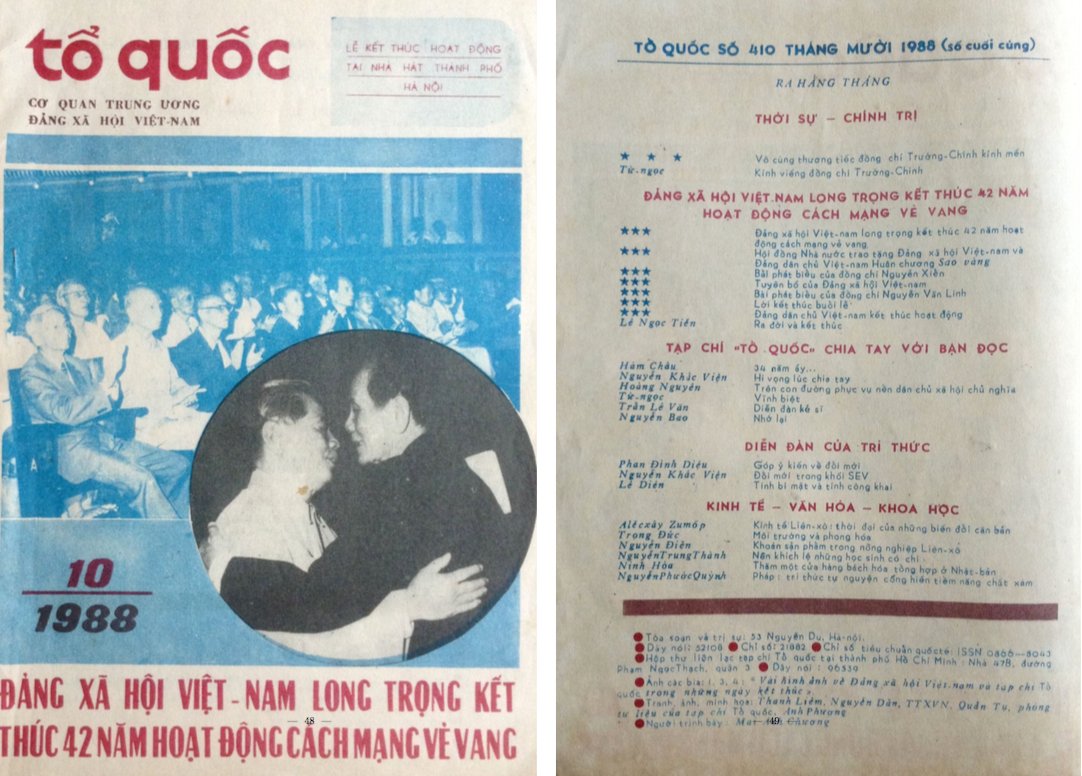
\includegraphics[scale=.3]{TQ88}
\end{figure}

Dưới tác động của cuộc cách mạng khoa học – kỹ thuật hiện đại, thế giới chúng ta đang trải qua những biến động và đổi thay cực kì sâu sắc\footnote{Bài này được viết trên cơ sở phát biểu ý kiến của tác giả tại một Hội thảo khoa học do một tiểu ban của Ban dự thảo Cương lĩnh tổ chức tại Ủy ban khoa học xã hội đầu năm 1988. Bài viết dự định sẽ được in trong một tuyển tập do tiểu ban nói trên ấn hành.}. Lực lượng sản xuất xã hội đang trong quá trình chuyển biến với những bước tiến cơ bản về chất lượng, nền kinh tế thế giới đang chuyển đổi “ từ một nền kinh tế chủ yếu dựa vào các nguồn tài nguyên cạn hẹp của hành tinh chúng ta sang một nền kinh tế của trí tuệ” - như lời người đứng đầu một cường quốc đã phát biểu. Loài người, với tất cả cái phức tạp và đa dạng, với tất cả những khác biệt sâu sắc và những mâu thuẫn giằng xé, đang tiến bước lên một giai đoạn lịch sử mới của nền văn minh.


Trong quá trình phát triển đó, thế giới càng ngày càng có nhiều mối ràng buộc để trở thành một hệ thống chỉnh thể. Đồng thời, trong cái chỉnh thể đó, chứa đựng nhiều cái khác biệt: trong khi một bộ phận tiên tiến của thế giới đã bước qua ngưỡng cửa đi vào giai đọa mới – giai đoạn thứ ba – của nền văn minh nhân loại, thì một bộ phận lớn khác vẫn chưa ra khỏi giai đoạn thứ nhất của lịch sử văn minh đó. Điều quan trọng là: \textit{chỉnh thể,} nhưng không \textit{thuần nhất}; đồng thời,\textit{ khác biệt}, nhưng không \textit{biệt lập.}


Đất nước ta, do nhiều nguyên nhân lịch sử, tiếc thay vẫn nằm trong bộ phận chậm tiến của nhân loại – ít nhất về phương diện kinh tế. Nhưng không biệt lập, nghĩa la vẫn tồn tại và tiến hóa trong sự tương tác với thế giới bên ngoài. Vì vậy, con đường mà ta muốn chọn cho mình phải là con đường trong cái “chỉnh thể” của thế giới đó. Cho nên, để xác định đường đi đúng đắn cho mình, ta phải hiểu rõ bản chất của những gì đang xảy ra trong thế giới, nói rõ hơn là bản chất của cuộc cách mạng khoa học – kĩ thuật và những đổi thay của thế giới hiện đại. Đó là điều thứ nhất. Điều thứ hai: chủ nghĩa xã hội – mục tiêu mà chúng ta hướng tới. Ngày nay, chúng ta không thể yên trí nói rằng chúng ta xây dựng chủ nghĩa xã hội, và thế là mục tieu đã rõ ràng. Ta biết rằng bản thân chủ nghĩa xã hội đang trải qua những thử thách nghiêm trọng. Vậy trong mô hình cũ của chủ nghĩa xã hội đã có những khuyết tật nào, và cần có quan niệm mới về chủ nghĩa xã hội đã có những khuyết tật nào, và cần có quan niệm mới về chủ nghĩa xã hội như thế nào. Không nghiên cứu kĩ những vấn đề này, thì cái đích mà chúng ta định sẽ mù mờ, và do đó, đường mà ta vạch ra cũng sẽ không xác đáng.


Dưới đây, nhằm mục đích trao đổi ý kiến, tôi xin phát biểu một số suy nghĩ và nhận thức về hai vấn đề quan trọng đó, và từ đó, một vài suy nghĩ về con đường trước mắt của ta.


\textbf{I – Cách mạng khoa học – kỹ thuật và thế giới hiện nay}


1 – Những phát minh khoa học trong thế kỉ 20 này, đặc biệt trong những thập kỉ gần đây, đã cho con người những hiểu biết sâu sắc về cấu trúc của vật chất, bản chất các dạng tồn tại và vận động của vật chất – trong các hệ thống của tự nhiên, sự sống và xã hội – từ đó tạo ra nhiều kĩ thuật mới làm thay đổi căn bản lực lượng sản xuất của xã hội.


Trước hết, đó là những phát minh của Vật lí học về cấu trúc của cật chất. những hiểu biết về cấu trúc hạt nhân, các phản ứng phân chia và tổng hợp hạt nhân đã là cơ sở cho kĩ thuật năng lượng hạt nhân. Các nghiên cứu về điện tử, về quá trình vận động của điện tử trong các môi trường vật chất khác nhau đã là nền tảng cho sự ra đời và phát triển nhanh chóng của kĩ thuật điện tử và vi điện tử. Với kĩ thuật điện tử, con người giải quyết được các vấn đề phức tạp về đo lường, khuếch đại, biểu diễn và biến đổi tín hiệu, đó là cơ sở của kĩ thuật xử lí thông tin, một ngành kĩ thuật tiến nhanh như vũ báo trong mấy chục năm qua.


Thông tin là một khái niệm trung tâm của khoa học trong thời đại chúng ta. Thông tin thể hiện mặt trật tự và tổ chức vật chất, vận động thông tin là hình thái chuyển hóa tính trật tự và tổ chức của các hệ thống vật chất. Sự ra đời và phát triển nhanh chóng của các ngành khoa học về thông tin, điều khiển, hệ thống, v.v…, cũng với những bước tiến vũ bão của kĩ thuật tin học là cơ sở vững chắc của quá trình “tin học hóa” các hoạt động của con người trong mọi lĩnh vực của sản xuất, kinh tế và xã hội.


Những phát minh sâu sắc cũng đã được thực hiện trong khoa học về sự sống – thí dụ việc phát hiện mã di truyền trong cấu trúc của đại phân tử ADN, việc tổng hợp gen, v.v… đó là cơ sở cho sự ra đời công nghệ sinh học, một ngành công nghệ hứa hẹn những đóng góp kì diệu phục vụ đời sống con người trong tương lai.
Không thể kể hết những thành tựu to lớn mà khoa học đã đạt được trong mấy thập kỉ qua trên mọi lĩnh vực của tri thức. Nói tóm lại một câu, khoa học một mặt đã đi rất sâu vào những cấu trúc cơ bản của các hệ thống vật chất, mặt khác, trên cơ sở những qui luật cơ bản đó nhận thức một cách sâu sắc các đối tượng thực tế của tự nhiên và xã hội, đồng thời tạo ra các công nghệ có tác dụng to lớn phát triển nền sản xuất và kinh tế của xã hội.


2 – Cách mạng khoa học – kĩ thuật hiện đại đang thúc đẩy sự phát triển vượt bậc với những thay đổi vè chất lực lượng sản xuất của xã hội.


Loài người đã trải qua hàng nghìn năm trong giai đoạn thứ nhất của nền văn minh – giai đoạn của \textit{nền sản xuất nông nghiệp thủ công}, với công cụ lao động chủ yếu là công cụ thủ công sử dụng nguồn năng lượng tự nhiên của cơ thể.


Giai đoạn thứ hai của nền văn minh nhân loại là giai đoạn của nền \textit{sản xuất cơ khí hóa}. Sự phát triển của giai đoạn này gắn liền với những thành tựu khoa học – kĩ thuật giúp con người khai thác và sử dụng các nguồn năng lượng to lớn trong thiên nhiên vào các hoạt động sản xuất. Tự động hóa các vận động cơ giới bằng cách sử dụng các nguồn năng lượng đó là đặc trưng chủ yếu của công cụ lao động trong giai đoạn văn minh cơ khí hóa.


Ngày nay với máy tính điện tử, với các thiết bị điều khiển tự động, với các rô bốt thông minh, loại người đang tiến đến giai đoạn thứ ba của nền văn minh nhân loại – sau khi các vận động cơ giới trong công cụ lao động đã được tự động hóa, thì lao động của con người trên những công cụ đó là để thực hiện các hoạt động điều khiển, tức là các vận động thông tin. Tự động hóa điều khiển, tức tự động hóa các vận động thông tin, là đặc điểm cơ bản của công cụ lao động trong giai đoạn này. Tuy nhiên, các quá trình thông tin không phải chỉ có trong hoạt động điều khiển các máy móc cơ khí, do đó phạm vi của việc tự động hóa cả quá trình thông tin rộng lớn hơn rất nhiều: trong sản xuất và tổ chức sản xuất, trong thông tin liên lạc, trong các hoạt động kinh tế như ngân hàng, tài chính, thống kê, kế hoạch, trong các hoạt động dịch vụ, trong điều tra cơ bản, nghiên cứu khoa học, trong công tác hành chính văn phòng, trong các hoạt động xã hội. v.v…


Ta biết rằng trong một nước công nghiệp phát triển, khu vực dịch vụ và thông tin càng ngày càng chiếm tỉ lệ to lớn trong nền kinh tế quốc dân (trong các nước tư bản chủ yếu, tỉ lệ đó hiện nay là trên dưới 60\%), vì vậy, tự động hóa các vận động thông tin, tức “tin học hóa” sản xuất và các hoạt động kinh tế - xã hội ó ý nghĩa cách mạng sâu sắc.


Sau giai đoạn cơ khí hóa là giai đoạn \textit{tin học hóa} – đó là sự chuyển biến về chất của lực lượng sản xuất xã hội, sự chuyển biến này kéo theo nó hàng loạt những chuyển biến khác về tính chất lao động sản xuất và kinh tế, về cơ cấu sản phẩm, cơ cấu tạo thành giá trị, cơ cấu của lực lượng lao động xã hội, v.v…


3. Trong nền kinh tế và xã hội của thế giới hiện đại đã và đang xảy ra những đổi thay cơ bản và sâu sắc trong cơ cấu nhu cầu, cơ cấu sản phẩm, cơ cấu phân bổ giá trị trong tổng thu nhập quốc dân, v.v…


Nền sản xuất đại công nghiệp cơ khí đã tạo ra những mối quan hệ ngày càng phức tạp, những mối liên kết ngày càng phong phú trong mỗi quá trình sản xuất cũng như trong toàn bộ nền kinh tế. Và đến lượt mình, bản thân các quan hệ, các mối liên kết đó cũng trở thành các yếu tố của chính quá trình sản xuất và hoạt động kinh tế, việc xử lý các mối liên hệ đó cũng trở thành một hoạt động sản xuất trực tiếp. Kinh tế phát triển thúc đẩy các nhu cầu xử lí thông tin hình thành và phát triển. đáp ứng các nhu cầu này lại làm cho kinh tế và xã hội càng có nhiều liên kết phong phú và đa dạng hơn, tức là đến lượt mình lại thúc đẩy thêm các nhu cầu xử lí thông tin, v.v…


Con người trong xã hội nói chung có hai loại nhu cầu: \textit{thức ăn và thông tin }(food and information). \textit{Thức ăn} (cách nói tắt cho các nhu cầu về ăn, mặc, ở,…) là nhu cầu để cá nhân tồn tại, thông tin là nhu cầu để con người trở thành thành viên của xã hội – xã hội càng phát triển, nhu cầu này càng tăng lên. Nhu cầu về \textit{thức ăn} là có hạn, còn nhu cầu về t\textit{hông tin} thì vẫn phát triển không ngừng.


Nhu cầu của con người, của sản xuất và của xã hội thay đổi, thì cơ cấu sản phẩm của nền kinh tế cũng thay đổi để đáp ứng các nhu cầu đó.


 Ta thấy rõ trong mấy chục năm gần đây, cơ cấu sản phẩm tiêu dùng của thế giới thay đổi nhanh chóng. Từ các máy thu thanh, thu hình đến máy tính cá nhân, điện thoại truyền hình, hộp thư điện tử, v.v…, các sản phẩm tiêu dùng đáp ứng các nhu cầu thông tin đang không ngừng tăng lên nhanh chóng về chủng loại, số lượng và chất lượng.
 
 
 Trong công nghiệp, các sản phẩm là tự liệu sản xuất, là công cụ lao động cũng chứa đựng ngày càng nhiều các yếu tố xử lí thông tin hay điều khiển tự động.
 
 
Quan niệm về vai trò của “công nghiệp nặng” hẳn sẽ có những thay đổi. Trong nền sản xuất cơ khí hóa, công nghiệp nặng về cơ bản là ngành chế tạo ra các máy móc cơ khí, tức các máy móc sử dụng năng lượng để thực hiện các vận động, cơ giới. Trong nền sản xuất “tin học hóa”, chế tạo máy sẽ cơ bản là chế tạo ra các máy xử lý thông tin. Và, vì vậy, nếu chế tạo máy trong giai đoạn cơ khí hóa được thực hiện trong các nhà máy lớn chế tạo công cụ của công nghiệp nặng truyền thống, “chế tạo máy” trong giai đoạn tin học hóa một phần lớn sẽ được thực hiện bằng lao động trí tuệ bên cạnh các máy tính điện tử, các “trạm làm việc” với máy tính và thiết bị tự động hóa thiết kế.


 Các sản phẩm đáp ứng nhu cầu thông tin trong các lĩnh vực kinh tế, văn hóa, và xã hội cũng chiếm một tỷ lệ rất to lớn trong nền sản xuất hiện đại.
 
 
 Cơ cấu nhu cầu, cơ cấu và tính chất của sản phẩm thay đổi, điều đó dẫn đến những đổi thay cơ bản trong cơ cấu phân bố các phần giá trị tạo thêm trong tổng thu nhập quốc dân. Xu hướng chung là trong những nền kinh tế càng phát triển và hiện đại hóa, thì phần đóng góp giá trị của các khu vực dịch vụ và thông tin càng có tỉ lệ lớn. Trong khi ở các nước chậm phát triển, nông nghiệp còn đóng góp trên 50\% giá trị trong thu nhập quốc dân, dịch vụ và thông tin không đáng kể, thì ở các nước tư bản phát triển, phần đóng góp giá trị của khu vực sản xuất nông nghiệp chỉ có khoảng 3-5\%, của khu vực dịch vụ 20-25\%, của khu vực thông tin 34-45\%. Ở đây, cần chú ý một điều là quan niệm về giá trị và việc tạo thành giá trị trong nền sản xuất xã hội cần có những thay đổi để phù hợp với bản chất của các quá trình sản xuất và kinh tế hiện đại.
 
 
 4 – Những thay đổi nói trên trong nền sản xuất xã hội đưa đến những đổi thay to lớn trong tính chất của lao động và cơ cấu thành phần lao động trong xã hội. Lao động chân tay thuần túy đã được thay thế phần lớn trong giai đoạn cơ khí hóa. Lao động điều khiển các máy móc cơ khí đã và đang được thay thế dần bởi các thiết bị điều khiển tự động hóa. Và, vì vậy, phần chủ đạo của lao động con người trong một nền sản xuất tương lai sẽ là lao động trí tuệ: thiết kế và tổ chức các hệ thống thông tin bằng máy tính, các hệ điều khiển và quản lý tự động hóa, thiết kế các máy tính, thế hệ mới, các loại thiết bị chuyên dụng, các hệ chuyên gia, các rôbốt thông minh, v.v… 
 
 
 Tất nhiên, nói như vậy không có nghĩa là lao động trong toàn xã hội sẽ là lao động trí tuệ. Chắc chắn sẽ vẫn còn những khâu nhất định của lao động chân tay, lao động điều khiển không thể tự động hóa hoàn toàn. Nhưng lao động trí tuệ có tính chất sáng tạo sẽ là lao động đặc trưng.
 
 
 Trong các hoạt động đó, cần đặc biệt chú ý loại hoạt động tổ chức và quản lí. Kinh tế và xã hội càng phức tạp, càng đa dạng, thì hoạt động tổ chức và quản lí sản xuất, kinh tế, xã hội càng khó khăn và có ý nghĩa cực kì quan trọng.
 
 
 Tính chất của lao động thay đổi, thì cơ cấu thành phần lao động của xã hội cũng thay đổi. Thành phần công nhân, đại diện cho chân tay và điều khiển các máy móc cơ khí, không còn đóng vai trò tiên tiến trong nền sản xuất xã hội nữa. Đại diện tiên tiến nhất của nền sản xuất hiện đại là lao động trí tuệ. Vì vậy, hoặc phải đổi mới bản thân khái niệm “công nhân”, hoặc phải đổi mới cách nhìn về “vai trò tiên tiến” của thành phần công nhân theo nghĩa truyền thống.
 
 
 Từ mười năm trước đây, nhiều nhà kinh tế học đã nhận định rằng ở các nước phát triển nhất, như Mĩ, “thông tin” là nguồn tài nguyên quốc gia quan trọng nhất. Gần đây, người ta lại nói: Thời đại của chúng ta đang chứng kiến một sự chuyển biến đến “một nền kinh tế của trí tuệ”. Với một vài phân tích sơ lược như trình bày ở trên, ta có căn cứ để tin vào sự thật đó.
 
 
 5 – Thế giới hiện đại, trong quá trình phát triển hết sức phức tạp và đa dạng, đang càng ngày càng trở thành một hệ thống chỉnh thể với tất cả những khác biệt và không thuần nhất trong bản thân nó.
 
 
 Thế giới bao gồm các quốc gia. Nói thế giới là một chỉnh thể có nghĩa là trong thế giới đó, có nhiều mối liên kết để cho sự tồn tại và phát triển của mỗi quốc gia luôn phụ thuộc và, và tác động đến sự tồn tại và phát triển của các quốc gia khác: và với những ràng buộc trong các tương tác và phụ thuộc đó, thế giới trở thành một thực thể hệ thống, có những thuộc tính hệ thống mà từng quốc gia thành viên không có. 
 
 
 Nền kinh tế hiện đại đang bước sang giai đoạn tin học hóa. Tuy nhiên, không hề có một nền kinh tế tin học hóa đối lập với một nền công nghiệp cơ khí hóa hiện đại. Đứng về toàn bộ quá trình phát triển mà nói, thì tin học hóa là giai đoạn tiếp nối trên cơ sở đã trải qua và đang hoàn thiện giai đoạn cơ khí hóa; và một nền kinh tế hiện đại hoàn chỉnh bao gồm trong nó các thành phần của nền sản xuất cơ khí hóa đang được tiếp tục hoàn thiện và các thành phần mới của “tin học hóa”. Bằng nhiều hình thức liên kết khác nhau, nền kinh tế hiện đại có xu thế trở thành một hệ thống hoàn chỉnh trên phạm vi thế giới, trong khi nền kinh tế của từng quốc gia không nhất thiết là hoàn chỉnh. Các mối quan hệ cân đối tương tác trong nền kinh tế cũng được thực hiện trong phạm vi toàn thế giới. Tính chỉnh thể của thế giới về mặt kinh tế đang được hình thành và củng cố như vậy.
 
 
 Khi hệ thống, tính chỉnh thể của thế giới được tăng cường, thì quan hệ giữa các quốc gia chủ yếu là quan hệ phụ thuộc lẫn nhau, sự tồn tại và phát triển của mỗi quốc gia có quan hệ gắn bó với sự tồn tại và phát triển của toàn hệ thống thế giới.
 
 
 Tính chỉnh thể làm xuất hiện những mục tiêu và lợi ích toàn cầu của toàn hệ thống, và độc lập với ý muốn con người, đó  là cơ sở cho một sự thống nhất nào đó giữa mọi quốc gia và thế lực có thể rất khác biệt nhau trong xã hội. Sự “thống nhất” lợi ích này lại càng được tăng cường bởi những lợi ích chung về mặt xã hội của toàn hệ thống thế giới khi toàn thế giới loài người đang cùng phải đương đầu với những nguy cơ thật sự đe dọa sự tồn tại của mình như chiến tranh hạt nhân hủy diệt, sự ô nhiễm và hủy hoại môi trường, v.v…
 
 
 Tất nhiên, các yếu tố làm cho thế giới trở thành chỉnh thể đó không hề làm cho thế giới trở thành thuần khiết. Các mâu thuẫn cơ bản của thời đại không mất đi, nhưng có những thay đổi nhất định về tính chất và phương thức giải quyết. Chẳng hạn, giữa hai hệ thống xã hội vẫn tồn tại những mâu thuẫn gay gắt, nhưng đồng thời cũng xuất hiện những mối quan hệ lợi ích phụ thuộc lẫn nhau; mâu thuẫn đó không thể giải quyết bằng chiến tranh, mà phải được giải quyết trong điều kiện cùng tồn tại hòa bình và thi đua hòa bình.
 
 
 Trong xu thế tăng cường các mối liên kết hệ thống đó của thế giới, mọi sự phân chia thế giới theo một tiêu chuẩn tuyệt đối hóa nào đó đều không tránh khỏi phiến diện. Các nước có cùng \textit{chế độ xã hội }có những quan hệ lợi ích liên kết với nhau, nhưng các nước có cùng \textit{trình độ phát triển} của nền sản xuất cũng có những vấn đề chung., và các mối quan tâm chung. Thí dụ: một nước chậm phát triển chọn nền xã hội chủ nghĩa có những lợi ích chính trị chung với các nước xã hội chủ nghĩa khác, nhưng về mặt sản xuất phát triển và kinh tế có tiếng nói chung với các nước chậm phát triển hơn là các nước xã hội chủ nghĩa đã phát triển.
 
 
 Trong thế giới chỉnh thể của vô vàn những mối liên kết phức tạp, những quan hệ hỗ trợ nhau cũng như những mâu thuẫn giằng xé nhau đó, một quốc gia, để tìm một chiến lược phát triển thuận lợi cho mình, phải tính đến tất cả các mối phụ thuộc, tìm kiếm một lối đi có lợi trong tất cả các mối phụ thuộc đó, chứ không thể đơn giản hóa, sơ lược hóa – và dó đó làm nghèo nàn – các mối liên hệ phụ thuộc của mình với thế giới.
 
 
\textbf{II. – Về chủ nghĩa xã hội}


1-	Hệ thống xã hội chủ nghĩa trên thế giới được bắt đầu hình thành từ sau thắng lợi của Cách mạng tháng Mười, đã trải qua một chặng đường dài xây dựng và đã có những cống hiến vĩ đại đối với sự tồn tại và phát triển của toàn nhân loại. Tuy nhiên, con đường xã hội chủ nghĩa là con đường chưa có sẵn, loài người đang phải dày công khám phá. Mô hình xã hội chủ nghĩa thực tế ở Liên-xô và các nước khác trong những thập kỉ qua đã chứng tỏ những ưu việt, đồng thời cũng bộc lộ những yếu kém mà gần đây càng thấy rõ.


 Cuộc cách mạng khoa học – kĩ thuật hiện đại đang làm rung chuyển thế giới, trên thực tế đã xảy ra và được tiến hành mạnh mẽ sâu rộng trong các nước tư bản phát triển, chứ chưa phải trong các nước xã hội chủ nghĩa, nó đang đi những bước chậm chạp và khó khăn. Chủ nghĩa xã hội, trên thực tế, trong những thập kỉ qua, chưa tạo được điều kiện thuận lợi cho những bước tiến mạnh mẽ của cách mạng khoa học – kĩ thuật, cho sự phát triển và đổi mới nền sản xuất và kinh tế của mình.
 
 
Như vậy, chủ nghĩa xã hội trên thế giới đang đứng trước những thử thách nghiêm trọng, cần có những đổi mới thật sự để khắc phục những yếu kém và phát huy được đầy đủ những ưu việt bản chất của mình. Để làm cơ sở cho những đổi mới đó, cần có những xem xét cơ bản về chính những nguyên tắc xây dựng chủ nghĩa xã hội hiện nay.


2-	Chủ nghĩa xã hội – theo định nghĩa – là giai đoạn quá độ tiến lên chủ nghĩa cộng sản. Để thủ tiêu chế độ bóc lột, giải phóng sức sản xuất xã hội, chủ nghĩa xã hội thực hiện chế độ sở hữu công cộng về tư liệu sản xuất, xây dựng một nền kinh tế kế hoạch hóa với chế độ quản lí tập trung của Nhà nước. Qui luật kinh tế cơ bản của chủ nghĩa xã hội xác định mục tiêu chung của nền kinh tế đó là mở rộng và hoàn thiện không ngừng nền sản xuất trên cơ sở kĩ thuật tiên tiến để thỏa mãn các nhu cầu ngày càng tăng và sự phát triển toàn diện của mọi thành viên trong xã hội. Nền kinh tế đó được phát triển theo qui luật cân đối và có kế hoạch. Trong chủ nghĩa xã hội, chưa có sự công bằng tuyệt đối những có sự công bằng xã hội ở giai đoạn thấp theo nguyên tắc phân phối theo lao động.


 Việc tổ chức và điều hành nền kinh tế theo kế hoạch háo nhà nước dưới sự quản lí tập trung đã có tác dụng đáng kể đối với việc xây dựng và phát triển nền kinh tế xã hội chủ nghĩa trong những giai đoạn nhất định và những hoàn cảnh nhất định.
 
 
Nhưng trong những thập kỷ vừa qua, cơ chế kinh tế theo những nguyên tắc nói trên đã bộc lộ những nhược điểm của nó, mà nhược điểm quan trọng nhất là không tạo ra được một động lực thật sự mạnh mẽ thúc đẩy sự phát triển năng động của nền kinh tế xã hội.


 Nhược điểm đó không nằm trong những mục tiêu tốt đẹp của chủ nghĩa xã hội, mà là trong những nguyên tắc không phù hợp với thực tiễn mà ta vẫn xem là những nguyên tắc (hay qui luật) của kinh tế xã hội chủ nghĩa.
 
 
 \textit{Động lực} phát triển kinh tế xét cho cùng, bao giờ cũng xuất phải xuất phát từ \textit{lợi ích kinh tế}. Xã hội gồm các thành viên là những con người cụ thể. Có lợi ích kinh tế của toàn xã hội và lợi ích kinh tế của mỗi cá nhân. Qui luật kinh tế cơ bản qui định trong nền kinh tế xã hội chủ nghĩa, lợi ích toàn xã hội là nhằm để phục vụ lợi ích của mọi thành viên. Từ đó, trong xã hội chủ nghĩa mỗi người trước hết phải phấn đấu cho lợi ích chung, lợi ích toàn thể, rồi sẽ có được trong lợi ích chung đó sự đáp ứng các lợi ích cá nhân chính đáng của mình. “Mỗi người vì mọi người, mọi người vì mỗi người” là nguyên tắc sống của xã hội. Tất cả những nguyên tắc đó \textit{đồng nhất lợi ích chung với lợi ích riêng}, trên thực tế dẫn đến không thừa nhận \textit{lợi ích riêng, phủ nhận cá nhân} và phủ nhận luôn cả nguồn động lực chân thực nhất của sự phát triển. Tuy nhiên, dẫu không được thừa nhận, thì về khách quan, lợi ích riêng vẫn tồn tại. Tồn tại, nhưng không được thừa nhận, dẫn đến những biểu hiện không thật, do đó cũng góp phần tạo ra cái “không thật” trong các mối quan hệ kinh tế, xã hội.
 
 
 Vấn đề lợi ích kinh tế là một vấn đề mấu chốt. Trong những năm gần đây, các nước xã hội chủ nghĩa đều có những điều chỉnh theo hướng thừa nhận tính độc lập lợi ích cá nhân và thực hiện các chính sách, biện pháp kết hợp lợi ích toàn xã hội và lợi ích các nhân. Chủ nghĩa xã hội có những tiền đề cần thiết cho sự kết hợp đó, đó là sự nhất trí về nguyên tắc lợi ích chung của toàn xã hội và lợi ích riêng của cá nhân người lao động. Nhưng cần thừa nhận một điều là: mỗi người lao động trong hoạt động sản xuất và kinh tế trực tiếp của mình nhằm trước hết đạt được lợi ích cá nhân. Còn tạo ra những biện pháp khống chế và hiệp tác như thế nào để các lợi ích cá nhân không mâu thuẫn, mà góp phần thực hiện lợi ích chung, là trách nhiệm quản lí của toàn hệ thống xã hội. Phải chăng khẩu hiệu lí tưởng “mỗi người vì chính mình, và từ chỗ vì chính mình mà góp phần vì xã hội”. Mỗi thành viên, được động lực lợi ích kích thích sẽ phát triển mọi năng lực năng động và sáng tạo của mình để tăng gia sản xuất và phát triển kinh tế, đồng thười toàn xã hội, bằng các biện pháp tổ chức và quản lí thích hợp, bằng các chế độ và chính sách thảo đáng, thực hiện sự hiệp tác “từ chỗ mỗi người vì chính mình mà góp phần vì toàn xã hội”.
 
 
 Hệ thống các yếu tố: một chế độ sở hữu công cộng về tư liệu sản xuất, một nền kinh tế Nhà nước được quản lí tập trung và phát triển theo kế hoạch, đã từng là nền tảng cho xã hội xã hội chủ nghĩa. Theo quan điểm của khoa học thông tin và hệ thống, một hệ thống kinh tế như vậy có những nhược điểm chính như sau:
 
 
-	Quản lí là làm quyết định trên cơ sở xử lí thông tin. Kế hoạch là quyết định của quản lí Nhà nước về hoạt động của toàn bộ nền kinh tế xã hội. Nếu muốn có những kế hoạch chi tiết thì phải cử lí thông tin về rất nhiều những mối quan hệ trong kinh tế - xã hội, mà \textit{độ phức tạp của chúng vượt quá khả năng của mọi hệ thống xử lí thông tin mà con người có thể có được}. Vì vậy, chỉ mới xét riêng nguyên nhân đó thôi, thì việc xác định một kế hoạch cân đối chi tiết cho toàn bộ nền kinh tế, về nguyên tắc là \textit{không thể được}. Không thể được: mà vẫn làm, thì kết quả là áp đặt lên nền sản xuất xã hội những “kế hoạch” không thực tế, buộc nền sản xuất đó hoặc phải tuân theo một cách khiên cưỡng để đi đến đổ vỡ, hoặc tự tìm cách thoát ra khỏi sự kiềm chế của “kế hoạch” để tạo nên \textit{hỗn loạn}.


-	Mọi kế hoạch đều mang tính chất là những mệnh lệnh tĩnh cho hệ thống kinh tế - xã hội là một hệ thống \textit{sinh động} với vô vàn những mối liên hệ phong phú và đa dạng. Bắt nền kinh tế tuân theo kế hoạch định sẵn là làm xơ cứng và nghèo nàn đi các mối liên kết sinh động đó. Trong khi bản thân các mối liên kết phong phú và đa dạng cũng đã tạo thành một yếu tố quan trọng của nền sản xuất xã hội, việc xử lí các mối liên kết mang lại những đóng góp to lớn vào giá trị tạo thêm trong nền kinh tế thì việc làm nghèo đi các mối liên kết là tước mất ở nền kinh tế những khả năng tạo thêm giá trị. Chính vì vậy mà trong khi ở các nước tư bản phát triển, khu vực dịch vụ và thông tin không ngừng tăng lên nhanh chóng (đóng góp trên dưới 60\% giá trị vào tổng thu nhập quốc dân, thì ở các nước xã hội chủ nghĩa, dịch vụ rất kém và khu vực thông tin cũng nghèo nàn.


-	Kế hoạch hóa cũng đi liền với \textit{độc quyền} Nhà nước trong mọi hoạt động sản xuất, kinh doanh. Một nền sản xuất không có cạnh tranh không được khuyến khích bởi sự đáp ứng các nhu cầu và thị hiếu của người tiêu thụ, thì tất yếu trở thành trì trệ, không đòi hỏi cải tiến và đổi mới một cách cấp thiết.


Ngoài những vấn đề kinh tế như trình bày trên, chủ nghĩa xã hội cũng đang phải xem xét lại nhiều vấn đề thuộc về hệ thống chính trị, đặc biệt là vấn đề dân chủ trong xã hội. Dân chủ là một yêu cầu cấp thiết để giải phóng và phát huy mọi năng lực sáng tạo của quần chúng trong sản xuất, trong quản lí kinh tế và quản lí Nhà nước. Trong lịch sử, dưới danh nghĩa chuyên chính vô sản đã không ít trường hợp thiết lập trong những thười gian dài sự chuyên chính của những phe nhóm thậm chí của những cá nhân. Tạo ra một cơ chế xã hội, một hệ thống chính trị bảo đảm không xảy ra những sự lạm dụng như vậy và bảo đảm cho một nền dân chủ thật sự - nền dân chủ trong đó mọi quyền lực trong xã hội thuộc về nhân dân – là một nhiệm vụ trọng đại trong công cuộc đổi mới hiện nay.


3. Để khắc phục các nhược điểm và để phát huy tính ưu việt bản chất của mình, chủ nghĩa xã hội cần được đổi mới. Nghiên cứu cơ sở lí luận cho sự đổi mới chế độ xã hội chủ nghĩa là một vấn đề cực kì quan trọng, chắc chắn đang được tiến hành ở nhiều nước. Dưới đây xin trình bày một vài suy nghĩa bước đầu.


   Trước hết, cần xem xét từ việc xác định \textit{mục tiêu}. Việc công hữu hóa, hợp tác hóa, quản lí tập trung, kế hoạch hóa, v.v… đều không phải là \textit{mục tiêu}, mà chỉ là \textit{phương tiện} mà ta đã từng hi vọng là đưa ta đạt tới mục tiêu. Mục tiêu của chủ nghĩa xã hội, xét cho cùng cũng là nhằm \textit{phát triển sản xuất} và tạo lập một sự \textit{công bằng xã hội}. Phát triển sản xuất trên cơ sở sử dụng có hiệu quả các thành tự khoa học và kĩ thuật tiên tiến để làm ra nhiều của cải vật chất và văn hóa đáp ứng các nhu cầu ngày càng tăng của con người và xã hội. Công bằng xã hội là một mối quan hệ xã hội không có áp bức bóc lột, mọi người lao động có điều kiện phát huy mọi năng lực sáng tạo của mình và được hưởng xứng đáng với thành quả lao động.
   
   
Hai mục tiêu đó không bao giờ cũng tương thích với nhau, và cơ chế đề đạt hai mục tiêu đó cũng rất khác nhau.


Không nhất thiết tương thích, có nghĩa là không phải khi mục tiêu này đạt được thì mục tiêu kia cũng đạt được, thậm chí có khi việc nhằm đạt mục tiêu này lại làm hỏng việc đạt mục tiêu kia. Chẳng hạn, trong điều kiện một nền sản xuất thấp kém, một nền kinh tế nghèo nàn thì không thể có công bằng xã hội. Trong điều kiện đó, nếu ta áp đặt một cách khiên cưỡng mục tiêu công bằng xã hội thì kết quả chỉ có thể là một thứ chủ nghĩa bình quân hình thức , không khuyến khích phát triển, thâm chí phá hoại sản xuất, rồi đến lượt mình điều đó lại dẫn đến hỗn loạn, làm cho ngay cả một sự công bằng bình quân trong nghèo đói cũng không đạt được. Mặt khác, trong chế độ tư bản, sự phát triển sản xuất  nhanh chóng rõ ràng cũng không nhất thiết dẫn đến công bằng xã hội. Tuy nhiên phải có một nền sản xuất phát triển ở trình độ cao, một nền kinh tế giàu có thì mới có điều kiện cần thiết cần thiết cho một sự công bằng xã hội thực sự. Vì vậy, trong sự kết hợp kết hợp hai mục tiêu nói trên, mục tiêu phát triển sản xuất bao giờ cũng cần được chú ý  một cách ưu tiên.


Cơ chế để phát triển sản xuất phải là cơ chế kích thích động lực lợi ích kinh tế, còn cơ chế để thực hiện công bằng xã hội lại thuộc phạm trù tổ chức và quản lí của Nhà nước.


Lấy lợi ích kinh tế làm động lực phát triển sản xuất tất nhiên dẫn đến việc có nhiều thành phần kinh tế khác nhau trong xã hội. Nhưng động lực lợi ích không phải chỉ liên quan đến các thành phần kinh tế cá thể, tư nhân, tập thể, mà cần phải kích thích động lực đó ngay trong thành phần kinh tế quốc doanh , tức là trong các xí nghiệp Nhà nước. Việc giành quyền tự chủ sản xuất và kinh doanh cho các xí nghiệp, tách quyền sở hữu của nhà nước với quyền quản lí kinh tế độc lập của xí nghiệp là những công việc có ý nghĩa quyết định theo phương hướng đó. Nền sản xuất xã hội, trong khung cảnh như vậy phải là một nền sản xuất hàng hóa với cơ chế thị trường theo đầy đủ ý nghĩa của nó.


Vai trò của Nhà nước xã hội chủ nghĩa trong kinh tế không còn là vai trò của một cơ quan quản lí tập trung, đưa ra các kế hoạch cho toàn bộ nền kinh tế, Nhà nước thực hiện chức năng của hệ thống , tức là những chức năng bảo đảm sự ổn định và phát triển của toàn hệ thống mà từng thành phần hoặc từng nhóm thành phần không thực hiện được. Theo nghĩa đó, trong quản lý kinh tế, kế hoạch quản lý kinh tế, kế hoạch nhà nước chỉ quan tâm đến các chỉ tiêu bảo đảm những cân đối lớn đối với kinh tế trong nước và trong kinh tế đối ngoại, trong khu vực sản xuất, đầu tư của Nhà nước chủ yếu tập trung vào những ngành tạo ra cơ sở hạ tầng cho sự phát triển và liên kết toàn hệ thống như: năng lượng, giao thông vận tải, thông tin liên lạc, nhà nước cần tập trung vào việc tìm kiếm và phát huy những nguồn tiềm lực lớn cho xã hội, đặc biệt là việc giáo dục, đào tạo các thế hệ trẻ và bồi dưỡng năng lực, nâng cao chất lượng cho người lao động trong xã hội.


Mục tiêu công bằng xã hội được Nhà nước thực hiện bằng các quy định pháp luật và các chính sách nhằm phân phối lại thu nhập quốc dân, tăng các khoản phúc lợi xã hội, tạo điều kiện cho mọi người lao động được giáo dục đào tạo và có cơ hội phát huy năng lực của mình.


Chủ nghĩa xã hội trên thế giới đã nhận thữ rõ những nhược điểm, những khuyết tật trong các mô hình cũ của mình. Một trong những vấn đề quan trọng nhất của quá trình đổi mới hiện nay là xây dựng cơ sở lí luận cho một xã hội xã hội chủ nghĩa với sức sống mới, phát huy được tính ưu việt thực sự của mình- mạnh mẽ, có sự công bằng xã hội theo nghĩa là mọi người lao động có điều kiện được phát huy mọi năng lực sáng tạo và được hưởng thụ xứng đáng với lao động của mình, một xã hội có nền dân chủ thực sự để mọi tư tưởng tiến bộ, mọi năng lực xuất sắc được được thể hiện và lựa chọn vào các vị trí xứng đáng vì sự phát triển và phồn vinh của toàn xã hội. Dĩ nhiên, có rất nhiều vấn đề phức tạp cần được nghiên cứu giải quyết trong việc xây dựng cơ sở lí luận cho một học thuyết đổi mới như vậy; trong bài viết ngắn này, tôi không có tham vọng đề cập đến nhiều.


4- Xin thêm vài lời về các nước chậm phát triển sau khi hoàn thành nhiệm vụ giải phóng dân tộc đã chọn con đường xã hội chủ nghĩa. Chủ nghĩa xã hội là một mơ ước nhưng trên thực tế, nền kinh tế-xã hội của các nước này hoàn toàn chưa có những chuẩn bị cần thiết cho việc xây dựng chủ nghĩa xã hội. Nhiều nước chậm phát triển, sau khi giành được độc lập, nôn nóng dán lên cho mình nhãn hiệu xã hội, chủ nghĩa, đã để mình lâm vào tình trạng khó khăn, mà chủ yếu là:


-	\textit{Về đối nội, } bằng cách áp đặt sự quản lí tập trung của Nhà nước, đã tự mình \textit{hạn chế}- nếu không nói là \textit{giết chết}-mọi năng lực làm ra của cái trong xã hội. Mục tiêu phát triển sản xuất, lẽ ra phải đặt lên ưu tiên số một, trong thực tế đã bị đặt dưới nhiều mục tiêu ảo tưởng khác. Hậu quả là đưa nên kinh tế-xã hội đến tình trạng rối loạn, chứa đựng nhiều dối trá, không dễ khắc phục nổi.


- \textit{Về đối ngoại}, tự làm mất đi nhiều mối quan hệ đáng lẽ cần phải có để phát triển; điều đó hạn chế khả năng giao lưu, tiếp thụ sức sống từ bên ngoài.


Một nước chậm phát triển chọn con đường xã hội chủ nghĩa, về khách quan mà nói, vẫn mang trong mình các yếu tố của sự chậm phát triển là chủ yếu, chứ không phải các yếu tố của chủ nghĩa xã hội là chủ yếu. Vì vậy, phải tìm cách sống và tự phát triển theo các qui luật khắc nghiệt dành cho tình trạng chậm phát triển, chứ không được ảo tưởng bỏ qua và vội áp đặt các qui luật của chủ nghĩa xã hội vốn chưa thích hợp với điều kiện yếu kém của mình. Chủ nghĩa xã hội là mơ ước, chứ chưa thế là hiện thực. Con đường quá dộ đến đó chắc không phải chỉ là một vài chục năm, và vì vậy không thể vì muốn “tiến thẳng” mà bất chấp mọi gai góc trên đường.


\textbf{III – Về con đường của ta}


Chúng ta đang xây dựng Cương lĩnh và chiến lược phát triển kinh tế - xã hội trong tinh thần đổi mới tư duy, đặc biệt là tư duy chính trị và tư duy kinh tế. Xác định một cách nhìn mới, không giáo điều bảo thủ, không lẹ thuộc vào vị trí quyền lực, thật sự khoa học, đối với con đường mà ta cần đi để thoát khỏi tình trạng khủng hoảng khủng hoảng và bế tắc nghiêm trọng hiện nay là hoàn toàn khẩn thiết.


Trong phạm vi bài biết ngắn này, và trong những hiểu biết hạn chế của mình, tôi không có tham vọng phát biểu ý kiến một cách toàn diện. Trong các phần trên, tôi đã trình bày, một số nhận thức đối với hai yếu tố có ảnh hưởng quan trọng đối với con người mà ta chọn cho mình: cuộc cách mạng khoa học – kĩ thuật hiện đại và chủ nghĩa xã hội. Trên cơ sở những nhận thức đó, tôi nghĩ rằng khi nghiên cứu để xác định Cương lĩnh và chiến lược cho mình, ta cần chú ý một số điểm sau đây:


1 - Xác định mục tiêu: Mục tiêu của ta là chủ nghĩa xã hội. Nhưng quan niệm về chủ nghĩa xã hội đang được đổi mới, ta cần có những thay đổi nhận thức về vấn đề này. Vả chăng, đối với chúng ta, một nước nghèo, đang trong tình trạng chậm phát triển, chủ nghĩa xã hội là mục tiêu mà ta hướng tới, chứ chưa phải là mục tiêu trực tiếp. Con đường quá độ đến đó còn rất dài, bao gồm nhiều chặng. Cần xác định mục tiêu cho những chặng trước mắt. Nghèo, chậm phát triển, thì mục tiêu cho những thập kỉ trước mắt phải được ưu tiên là phát triển sản xuất, thoát khỏi nghèo nàn và lạc hậu. \textit{Bằng mọi cách} để phát triển sản xuất, làm ra nhiều của cải cho xã hội là điều cần thiết nhất lúc này. Để đạt được mục tiêu “hiền lành” đó, thì những khẩu hiệu “ai thắng ai”, những quan hệ căng thẳng vô mục đích là không thích hợp.


2 - Ta đang đi theo hướng tháo gỡ các ràng buộc để thành phần kinh tế tham gia vào phát triển sản xuất của xã hội. Nhưng để thật sự phát triển sản xuất cần khẳng định một cách đầy đủ hơn một cơ chế mới của nền kinh tế xã hội. Một nền sản xuất hàng hóa với cơ chế thị trường không thể thật sự thúc đẩy sản xuất nếu chỉ là hàng hóa nửa vời, thị trường nửa vời. Không thể chỉ xem sản phẩm là hàng hóa, trong khi vật tư, lao động, vốn… còn chưa là hàng hóa. Không thể để các xí nghiệp được tự chủ kinh doanh khi vẫn độc quyền sản xuất, không có cạnh tranh, v.v… Ta không sợ phát triển sản xuất với một nền sản xuất hàng hóa đầy đủ là làm mất chủ nghĩa xã hội, bởi vì chủ nghĩa xã hội là cái ta đã có đâu mà sợ mất. Có mất chăng là mất đi những thứ mang nhãn hiệu chủ nghĩa xã hội dối trá, để xây dựng dần cơ sở giúp có cho một chủ nghĩa xã hội thật sự trong tương lai.


3 - Như một phần trên đã nói, thế giới ngày nay là một chỉnh thể, và cái chỉnh thể đó đang bước mạnh sang giai đoạn thứ ******** của nền văn minh nhân loại. Ta phải tìm đường cho ta với tư cách là một thành viên trong cái chỉnh thể đó. Như vậy, ta không tự đặt cho mình việc xây dựng một nền kinh tế độc lập, hoàn chỉnh và tự cân đối. Ta là một bộ phận của thế giới và tự tìm vị trí của mình trong cái cân đối chung của hệ thống. Vị trí nào có lợi nhất? Điều đó phụ thuốc vào năng lực của ta. Nếu ta có tiềm lực trí tuệ lớn thì có thể xông đến những lĩnh vực mũi nhọn của thời đại. Trong khi chưa có, thì làm những công việc lao động có tính chất “làm thuê” cũng là cần thiết. Việc tìm ra cho được trong sự liên kết của chỉnh thể thế giới đó những mối liên hệ kinh tế khả dĩ đưa lại giá trị cao nhất là nội dung chủ yếu của việc xác định chiến lược.


4-	Xu thế phát triển của thế giới là tiến đến một nền kinh tế của trí tuệ. Trong khi đang phải giải quyết những nhiệm vụ của một nền kinh tế chậm phát triển, nếu muốn được “vượt giai đoạn”, tức là muốn tiến nhanh, việc tạo ra  một năng lực trí tuệ lớn của dân tộc là điều cực kì quan trọng. Hệ thống giáo dục đào tạo, nghiên cứu khoa học phải được đặc biệt quan tâm đầu tư và phát triển. Bất cứ một chính sách thiển cận nào trong lĩnh vực này cũng đều mang lại những thiệt hại to lớn không bù đắp nổi cho đất nước trong tương lai.


5-	Để phát huy mọi năng lực sáng tạo, mọi tư tưởng và sáng kiến, để dân tộc luôn luôn lựa chọn được những tài năng thật sự vào những vị trí xứng đáng của hệ thống làm quyết định, cần phải xây dựng được một nền dân chủ xã hội, nền dân chủ bảo đảm điều đã ghi trong Hiến pháp là “ở nước ta mọi quyền lực đều thuộc về nhân dân”.

\begin{flushright}

\textbf{P.Đ.D}
\end{flushright}



%
%
%\chapter{Báo Tổ Quốc số 08/89 : Góp Ý Kiến Về Đổi Mới (08/1989)}\index{Báo Tổ Quốc,Báo chí}
%  \includepdf[pages=1-,noautoscale,pagecommand={\thispagestyle{plain}}]{Docs/1988_ToQuoc_bia_so_cuoi.pdf}
%  \includepdf[pages=1-,noautoscale,pagecommand={\thispagestyle{plain}}]{Docs/1988_GopYKienVeDoiMoi_ToQuoc_10_88.pdf}
\newpage
\begin{center}
\Large Nhớ lại
\end{center}
\begin{flushright}
Kính tặng các đồng chí ở Đảng xã hội và báo <<Tổ Quốc>>\\
 cùng thầy Nguyễn Lân kính mến,
\end{flushright}
Bao năm tháng sống trong lòng <<XÃ HỘI>>\\
Từ vành nôi <<TỔ QUỐC>> sớm trưởng thành \\
Như cánh chim hướng bình minh bay tới\\
Nay trở về nhớ lại những ngày xanh.\\
Chẳng thể quên những tháng ngày đầm ấm\\
Bàn tay ai dìu dắt nặng ân tình\\
Chim bay chuyền hay giữa trời tung cánh\\
Vẫn trong lòng <<TỔ QUỐC>> mông mênh.\\
\begin{flushright}
16-10-1988\\
NGUYỄN BAO
\end{flushright}

\newpage
\begin{center}
 \Large GÓP Ý KIẾN VỀ ĐỔI MỚI
 \end{center} 
\begin{flushright}
PHAN ĐÌNH DIỆU
\end{flushright}
\begin{figure}
\centering
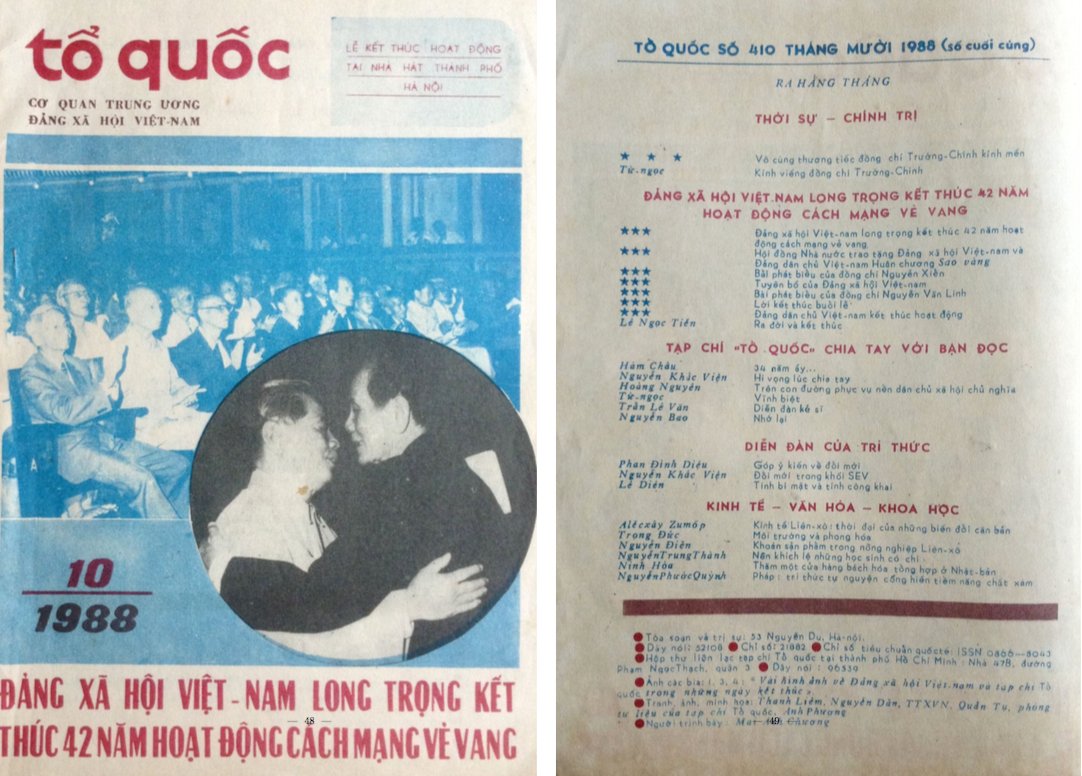
\includegraphics[scale=.3]{TQ88}
\end{figure}


L.T.S-\textit{Tháng chính 1986, tại Hội nghị Ủy ban trung ương Mặt trận Tổ quốc Việt Nam góp ý kiến với Đại hội VI của Đảng cộng sản Việt Nam, giáo sư Phan Đình Diệu, tiến sĩ khoa học toán-lí đã đọc một bản tham luận . Từ đó đến nay, hai năm đã trôi qua, thời gian chỉ càng làm sáng tỏ thêm sự đúng đắn của những ý kiến mà tác giả đã nêu lên trong bản tham luận ấy. Đó là những ý kiến được đề xuất từ sự suy nghĩ độc lập với tầm nhìn xa rộng của một người tri thức có nhiệt tâm và hiểu biết về nhiều lĩnh vực.}


\textit{Tạp chí << Tổ quốc>> trân trọng giới thiệu với bạn đọc nguyên văn bản tham luận ấy.}



Đất nước ta đang ở một thời đểm mà sự sống còn và phát triển của nó đòi hỏi phải có bước ngoặt của sự đổi mới toàn diện. Với ý thức trách nhiệm của một người dân đối với đất nước, tôi xin phép được góp một số ý kiến sau đây:


1-	\textit{Đổi mới tư duy}: Ta kêu gọi nhiều về đổi mới tư duy. Nhưng \textit{nội dung} của sự đổi mới như thế nào thì không thấy nói rõ. \textit{Mới} là thế nào? Cơ sở của sự đổi mới là gì? Tôi nghĩ cần xây dựng một hệ thống lí luận cho sự đổi mới này. Có thể một số yếu tố sau đây phải được coi là căn cứ khoa học của nội dung đổi mới tư duy:


a.	Những luận điểm cơ bản của học thuyết mác xit về kinh tế và về chủ nghĩa xã hội khoa học vẫn là căn cứ quan trọng cho tư duy đúng đắn của chúng ta. Tất nhiên cái mới lạ ở chỗ không biến mỗi lời của Marx, Engels Leenin thành một giáo điều, mà phải nghiên cứu một cách khoa học. Trong sự nghiên cứu đó, cần hiểu sâu sắc hơn các nguyên lí cơ bản, đồng thời cần xem xét lại một số luận điểm hoặc nhận định không còn phù hợp với thực tiễn của thời đại ngày nay. Nói cách khác, cần nghiên cứu nó như một học thuyết khoa học.


b.	Những tư tưởng lớn, những quan điểm và phương pháp nhận thức mới mà cuộc cách mạng khoa học- kĩ thuật hiện nay mang lại. Đây lả một yếu tố cực kì quan trọng. Thí dụ: quan điểm hệ thống, các tư tưởng và phương pháp của khoa học điều khiển hiện đại cho ta những khả năng nhìn nhận và phân tích mới mẻ đối với các hệ thống kinh tế-xã hội. Tri thức khoa học của thời đại là một nguồn phong phú cung cấp sức sống mới cho tư duy và nhận thức của chúng ta.


c.	Những nhận thức lí luận trên cơ sở phân tích thực tiễn phát triển của thế giới hiện đại như: vai trò của cách mạng khoa học- kĩ thuật: những điềm hay, dở cũng như sự vận động của các hình thái tổ chức xã hội hiện tại, những thử thách nghiêm trọng đối với sự phát triển  mà chủ nghĩa xã hội thực tế đang gặp phải, kinh nghiệm của các nước trong thế giới thứ ba, xu hướng phát triển của thế giới và quan niệm mới về chủ nghĩa xã hội,v....v


Cần xây dựng dần một hệ thống lí luận như vậy để làm nền tảng khoa học cho sự đổi mới tư duy.


Với cách tiếp cận đó đối với <<đổi mới tư duy>>, tôi xin đề cập đến một số vấn đề sau đây:

2-	\textit{Đánh giá tình hình và thực trạng xã hội}:


Tình hình kinh tế-xã hội của ta đang rất khó khăn, nghiêm trọng, đó là điều ai cũng biết. Nhưng đặc điểm cơ bản là gì? Tôi nghĩ rằng đặc điểm cơ bản là: Nhà nước tập trung độc quyền nhưng bất lực, trog khi đó xã hội phát triển hỗn loạn ngoài phạm vi kiểm soát của Nhà nước. Về tổ chức và quản lí kinh tế, một nhà nước nắm trong tay mọi quyền lực và phương tiện, mà làm ăn thua lỗ, không trả lương được cho người làm công đủ sống, thì rõ ràng về mặt kinh tế, một nhà nước như vậy không thể tiếp tục tồn tại.


Những tiêu cực hiện nay trong xã hội và trong Nhà nước là hiện tượng hay bản chất? một hiện tượng lặp đi lặp lại, có tính phổ biến thì rõ ràng mang tính bản chất. Vậy bản chất ấy là gì? Là đã áp đặt lên một thực thể những nguyên tắc không phù hợp với khả năng vận động và phát triển khách quan của nó, trong khi trên thực tế sự phát triển của thực thể đó vẫn cố tìm cách thoát khỏi sự áp đặt, để tuân theo những <<quy luật>> thích hợp với nó.


Xã hội ta chưa phải là xã hội chủ nghĩa. Cưỡng bức những kiều xã hội chủ nghĩa một cách <<ý chí luận>> cho nó như vừa qua thì không làm cho nó gần tới chủ nghĩa xã hội, mà thực tế đẩy nó ra xa hơn.


3-	\textit{Thế giới là gì? Ta là gì? Nên đặt mục tiêu gì cho nước ta hiện nay?}


Với quan niệm <<ta>> không hải là một hệ thống lớn hơn là thế giới, muốn tìm cách phát triển, ta cần phải nghiên cứu kĩ các vấn đề nói trên.


a.	Thế giới đã và đang có những biến đổi to lớn. Cách mạng khoa học-kĩ thuật hiện đại đang làm thay đổi nhanh chóng lực lượng sản xuất và tất nhiên ảnh hưởng đến sự biến đổi quan hệ sản xuất. Cơ cấu sản phẩm, cơ cấu tạo thành giá trị có những thay đổi lớn (thí dụ: các khu vực thông tin và dịch vụ chiếm tỉ lệ ngày càng lớn trong thu nhập quốc dân), nhu cầu của con người cũng có nhiều thay đổi. Tính chất xã hội, tính toàn cầu của nền sản xuất và kinh tế và ngày càng lớn, do đó, khái niệm <<độc lập>>  thay đổi ý nghĩa ( có còn indespeendance hay chỉ inberdépendance?).v....v


b.	Ta là gì trong thế giới đó? Đã cần xác định là một nước xã hội chủ nghĩa chưa? Trong thực tế, ta chưa thể tự xem là một nước xã hội chủ nghĩa, mà làm ai có chủ nghĩa xã hội trên cơ sở một nền kinh tế ốm yếu, một xã hội nghèo đói.


Rõ ràng ta là một nước nghèo trong thế giới thứ ba- chủ nghĩa xã hội là một mục tiêu xa mà ta muốn đạt đến chứ chưa phải là một hiện thực.


Xác định đúng vị trí là rất quan trọng- một mặt mình tự nhìn rõ mình, mặt khác tranh thư được sự đồng tình và ủng hộ của thế giới.


c.	Cách xác định vị trí của ta trong thế giới sẽ giúp ta xác định được mục tiêu cho sự phát triển của mình.


Là một nước nghèo, chậm phát triển, thì rõ ràng mục tiêu trước mắt phải là tìm dược điều kiện yên ổn để làm ăn, thoát khỏi cảnh nghèo. Thoát khỏi cảnh nghèo nàn , tạo ra nhiều giá trị, đó phải là mục tiêu ưu tiên. Phải chăng trong thời gian qua ta đã theo đuổi nhiều mục tiêu vượt quá khả năng thực tế của ta và đã phải trả giá đắt mà mục tiêu vẫn không đạt được?


4-\textit{	Các giải pháp cho ngắn hạn}:


Ta nhấn mạnh đến mục tiêu <<ổn định>>. Nhưng rõ ràng không thể có ổn định trong tình trạng tổ chức kinh tế-xã hội hiện nay. Chỉ có thể tìm sự ổn đinh trong một sự thay đổi, một sự biến chuyển cơ bản về tổ chức và quản lí kinh tế-xã hội theo hướng giải phóng và phát huy mọi thứ khả năng làm ra của cải của xã hội. Được (và phải) làm việc, làm đủ ăn, lương đủ sống và điều kiện tối thiểu cho sự ổn định và phát triển.


Trên tinh thần đó, cần phát triển rộng rãi khu vực kinh tế thập thể,cá nhân và tư nhân, kinh tế gia đình. Cần khẳng định bằng pháp luật chính sách lâu dài đối với sự phát triển các khu vực kinh tế này. Bằng các chính sách đó, giải phóng mọi khả năng sản xuất hiện có ở trong nước, thu hút sự đóng góp của Việt kiều ở ngoài nước và các nguồn khác.


Nhà nước giảm bớt và thu hẹp khu vực sản xuất và kinh doanh do mình trực tiếp nắm mà không có lãi. Chỉ nên giữ lại một số ngành và cơ sở sản xuất then chốt đối với kinh tế quốc dân. Trong các xí nghiệp nhà nước, chế độ tự chủ kinh doanh nên đến đâu?


Cần tách quyền sở hữu và hoạt động quản lí tài sản thuộc quyền sở hữu nhà nước, nhưng xí nghiệp cần được hoàn toàn tự chủ trong việc quản lí hoạt động sản xuất, kinh doanh, Nhà nước chia phần lợi nhuận và thu thuế. Những ngành xây dựng cơ sở hạ tầng mà Nhà nước cần tập trung phát triển là: năng lượng, giao thông vận tải, đặc biệt thông tin-liên lạc.


Để phát triển kinh tế theo các hướng đó, từ chỗ thử nhận các lợi ích kinh tế khác nhau. Phải tiến lên thừa nhận sự cạnh tranh- cạnh tranh trong khu vực kinh tế tư nhận, và cả cạnh tranh trong khu vực Nhà nước: việc phá sản do làm ăn thua lỗ của các xí nghiệp, quốc doanh cũng cần xem là tự nhiên!


Bằng việc phát triển mọi thành phần kinh tế trong xã hội. Nhà nước mới có khăng thu hẹp biên chế. Cũng cần nhanh chóng có chính sách đối ngoại thích hợp để giảm chi phí quốc phòng, giảm quân đội. Tăng thu nhập cho ngân sách và giảm biên chế ăn lương thì Nhà nước mới sớm có khả năng trả lương đủ sống cho những người làm việc trong bộ máy nhà nước.


5-\textit{	Hướng tìm giải pháp cho lâu dài}:


Về quan niệm, cần đặt ra trong thế giới để tìm kiếm giải pháp. Như vậy không phải đi tìm một sự phát triển cân đối trong nội bộ nước ta như một hệ kín, mà cần nghiên cứu sự phát triển <<cân đối>> của thế giới và trong hệ lớn của thế giới đó, ta có thể và nên làm gì để phát huy được hết khả năng và thu nhiều lợi nhất. Do đó, trong khi chưa đủ khoai ăn, không nhất thiết chỉ đi trồng khoai, mà nhiều khi phải học để làm chim quay, làm chim quay bán cho người khác ăn để lấy tiền mua khoa cho con mình ăn-mà có nhiều tiền thì rồi mới dần thoát khỏi cảnh ăn khoai, chứ nếu chỉ trồng khoai thì suốt đời chỉ được ăn khoai!


Với cách đặt vấn đề như thế, cần nghiên cứu xu thế biến đổi và phát triển của cơ cấu kinh tế thế giới, cơ cấu hình thành và tạo ra giá trị trong các khu vực sản xuất, dịch vụ của kinh tế thế giới, sự biến đổi của nhu cầu con người và do đó nhu cầu thị trường trong hiện tại và tương lai.


Một đặc điểm trong sự biến đổi cơ cấu đó là khu vực dịch vụ và thông tin ngày càng chiếm một tỉ lệ lớn trong tổng giá trị của kinh tế các nước phát triển, hàm lượng trí tuệ trong các loại sản phẩm ngày càng tăng. Nhu cầu của con người hiện tại và tương lai là thức ăn và thông tin. Nhu cầu về thức ăn thì có hạn, còn về thông tin thì chưa có giới hạn.


Ta cần chuẩn bị gì cho Việt Nam hòa nhập được vào thế giới trong tương lai, và trong sự hòa nhập đó, tìm được cho mình một chố đứng chắc chăn, có lợi.


Rõ ràng trong khi đang cần chú trọng phát triển nông nghiệp, công nghiệp, hàng tiêu dùng..v.. cũng cần chú ý ngay đến việc tạo điều kiện cho sự phát triển các ngành dịch vụ và các ngành làm ra các sản phẩm trong khu vực thông tin, các ngành đòi hỏi chất lượng trí tuệ. Việc làm ra tiền nhờ các hoạt động trí tuệ cần được phát triển, kể cả việc xuất khẩu lao động trí óc sang các nước đang phát triển hiện nay.


Muốn vậy, cần phải cải tổ hoàn toàn và đầu tư mạnh cho hệ thống giáo dục , đào tạo và nghiên cứu khoa học. Việc đào tạo giáo viên, bác sĩ để xuất khẩu cũng cần được đầu tư thích đáng và có hệ thống. Cần có chính sách và đầu tư thích đáng cho các ngành như điện tử và tin học, công nghệ sinh học..v..v


Chú ý rằng ngay đối với nông nghiệp và hàng tiêu dùng cũng cần được phát triển theo hướng hiện đại hóa các loại sản phẩm hàng hóa được làm ra.


Tạo tiềm năng tri thức và tri tuệ cho dân tộc là cực kì quan trọng. Hạn chế quá trình đó sẽ là một tội lỗi đối với dân tộc trong tương lai!


Tất nhiên, để làm được các việc trên, một điều kiện tiên quyết là phải thực sự biến nước ta thành một hệ mở, mở với thế giới và hòa nhập vào thế giới như một thành viên không bị phân biệt đối xử.


6-	\textit{Về chính sách đối ngoại}:


Đây là một lĩnh vực tế nhị, tôi không biết gì nhiều và không dám nói nhiều. Nhưng có những điều cấp bách mà ai cũng mong được sớm giải quyết.


Với mục tiêu là sớm thoát khỏi cảnh nghèo để phát triển đất nước hiện nay, rõ ràng ta càng cần nhiều bạn ít thù. Bạn, thù ra sao phụ thuộc rất nhiều vào cách ta xác định mục tiêu và cách sống của ta. Nếu ta tự xem là một nước chậm phát triển, với mục tiêu tìm sự yên ổn để khắc phục nghèo nàn và vươn lên, thì chắc sẽ nhiều bạn ít thù hơn. Nếu ta tự xem là mạnh, với mục tiêu lật đổ chủ nghĩa tư bản trên thế giới (đấy là giả dụ thôi) thì trong điều kiện thế giới hiện tại, chắc là khó mà có nhiều bạn.


Trong khung cảnh đó, giải quyết vấn đề Campuchia và quan hệ Trung Quốc là điềm quyết định nhất. Tôi chắc Trung Quốc sau này vẫn có những mưu đồ của một nước lớn, nhưng Trung Quốc có kẻ thù hay không là kẻ thù cũng một phần phụ thuộc vào cách đặt mục tiêu của ta trong khu vực này. Liên Xô xem Trung Quốc là một nước xã hội chủ nghĩa láng giềng vĩ đại. Mọi nước xã hội chủ nghĩa khác đang tìm quan hệ thân thiện với Trung Quốc. Trung Quốc ngày này không phải như thời cách mạng văn hóa. Phải chăng trong mấy năm qua, Trung Quốc đang khám phá con đường con đường đưa một nước lớn chậm phát triển và hỗn loạn đi lên con đường ổn định, thoát dần khỏi nghèo nàn và vươn lên hiện đại, trong khi vẫn giữ mục tiêu xa là chủ nghĩa xã hội? Vậy thì, bình thường hóa, lập quan hệ hữu nghị và học Trung Quốc là điều đáng mong muốn.


Tất nhiên không dễ nhưng rõ ràng quan hệ với Trung Quốc là một vấn đề sống còn của chúng ta. 


7-	\textit{Vấn đề dân chủ}:


Để đổi mới thì cần có dân chủ trong xã hội. Mà dân chủ cũng phải là một mục tiêu của sự đổi mới.


Việc xây dựng một nền dân chủ xã hội chủ nghĩa hay nói đúng hơn, một chế độ xã hội chủ nghĩa thự sự dân chủ, là một vấn đề cực kì quan trong của thời đại, chắc chắn là còn cần nhiều nghiên cứu, thề nghiệm và đấu tranh đề đạt tới.


Dân chủ là quyền làm chủ của người dân. Trong xã hội, một người dân vừa là cá nhân mình, vừa là một thành viên của xã hội. Quyền làm chủ, với tư cách cá nhân, là quyền sống, quyền mưu cầu hạnh phúc, quyền tự do thân thể, tự do tư tưởng..v...v.. Với tư cách là một thành viên của xã hội, quyền làm chủ là quyền tham gia làm quyết định trong mọi vấn đề tổ chức và quản lí xã hội. Nhưng việc làm quyết định không thể mọi người đều làm mà phải ủy thác cho lãnh đạo. Vì vậy, ở đây dân chủ được thể hiện ở quyền tham gia tự do lựa chọn các cơ quan lãnh đạo, đặc biệt là lãnh đạo cao nhất của đất nước và quyền công khai giám sát, phê phán, tranh luận và đánh giá quyết định của lãnh đạo đương nhiệm. Để thực hiện các quyền đó cần được thực sự tự do ứng cử và bầu cử, tự do ngôn luận đặc biệt là tự do báo chí, tự do hội họp và lập hội,v.v. Điều kiện để thực hiện các quyền đó là bảo đảm tính công khai về mọi thông tin trong xã hội: nói cách khác, đó là quyền bình đẳng về sở hữu thông tin trong xã hội.


Dân chủ là quyền của dân, đồng thời cũng là nguồn vô tận nên tạo nên sự phong phú và giàu có của xã hội. Vì vậy, dân chủ là một yêu cầu cấp thiết, một nội dung cơ bản của đổi mới.


8-	\textit{Vấn đề đoàn kết dân tộc}:


Nhiệm vụ của Mặt trận Tổ Quốc chúng ta luôn luôn là đoàn kết dân tộc để xây dựng và bảo vệ đất nước. Vì vậy, hơn lúc nào hết, trong thời điểm hiện nay, cần tập hợp được cao nhất tất cả lực lượng của dân tộc để phấn đấu cho sự phồn vinh của đất nước.


Tuy nhiên, ta cũng cần nhìn nhận rằng tuy thống nhất đất nước đã được mười năm, nhưng dân tộc và đất nước chưa thật sự được thống nhất một cách mạnh mẽ: lòng người còn phân tán, Bắc –Nam còn nhiều phân biệt, tình trạng địa phương cát cứ trầm trọng, nhiều vấn đề sau chiến tranh còn nhức nhối , còn nhiều phân biệt đối xử trong các tầng lớp nhân dân, dòng người bỏ đất nước ra đi còn tiếp diễn,.v..v.. nhưng quan trọng nhất là sức mạnh của dân tộc (về trí thức, về kinh tế, về khả năng sản xuất kinh doanh, ở trong nước và ngoài nước) chưa được huy động cho sự phát triển đất nước. 


Một chính sách đoàn kết dân tộc rộng rãi cần được ban bố và thi hành trong thực tế. Cốt lõi của chính sách đó phải là: mọi người Việt Nam, dù ở góc trời nào, miễn là có nguyện vọng, đều có thể tìm được một chỗ đứng bình đẳng trên đất nước Việt Nam này để lao động và cống hiến cho sự phồn vinh của đất nước bằng mọi cách thích hợp với hoàn cảnh và khả năng của mình. Và tất nhiên, điều đó sẽ được thể hiện bằng những chính sách cụ thể, như về giải quyết các hậu quả sau chiến tranh còn tồn tại, chính sách đối với người Việt Nam ở nước ngoài, chính sách thu hút vốn đầu tư và thu hút lực lượng khoa học kĩ thuật..v..v..


Tôi hi vọng rằng một số ý kiến trên đây sẽ được xem là phần đóng góp giọt nước nhỏ bé của mình vào trong hơn 60 triệu giọt nước khác của dân tộc để hòa thành dòng thác đổi mới của đất nước ta hiện nay.

\chapter{Số báo cuối của Báo SGGP năm 1989 : Dân Chủ Và Việc Phát Huy Nguồn Của Cải Trí Tuệ Của Dân Tộc (08/1989)}\index{Báo SGGP,Báo chí}
%\input{LoiDan/1989_Loidan_danchu_SGGP}
%  \includepdf[pages=1-,noautoscale,pagecommand={\thispagestyle{plain}}]{Docs/1989_Dan_chu_va_su_phat_huy_nguon_cua_cai_tri_tue_cua_dan_toc.pdf}

Dân chủ là một yêu cầu lớn của thời đại, cũng là một nội dung lớn của công cuộc đổi mới đang được tiến hành trên đất nước ta hiện nay. Dân chủ vừa là quyền lợi của từng công dân, vừa là điều kiện của sự phát triển của xã hội. Chúng ta đã nhận thức rõ ràng để đổi mới thì cần có dân chủ, và dân chủ cũng phải là một mục tiêu của đổi mới. Tuy nhiên, do hoàn cảnh lịch sử, xã hội ta chưa có được truyền thống  dân chủ, vì vậy, đối với chúng ta, ngày nay dân chủ còn là một bài học rất mới mẻ, chắc là còn cần nhiều khảo cứu lý luận và thể nghiệm thực tiễn để dần đi đến hoàn thiện.


Mỗi người, tùy chỗ đứng vốn có của mình, có thể có cách nhìn riêng đối với yêu cầu dân chủ. Phải chăng vì vậy mà trong thời gian qua, khi đề cập đến dân chủ, có người nghĩ đến phải chống phá một cái gì đó, lại có người sợ bị chống phá một cái gì đó ; cho nên dễ có xu hướng hỗn loạn , mà cũng dễ có nguy cơ quay về với bảo thủ. Để có một cách nhìn chung – chỗ đứng chung đó là lợi ích của dân tộc, là yêu cầu phát triển của đất nước, trong giai đoạn hiện nay là yêu cầu giải phóng và phát huy mọi năng lực làm ra của cải  của xã hội để nhanh chóng thoát khỏi nghèo nàn lạc hậu và vươn dần lên sự giàu có phồn vinh cho đất nước. Dân chủ là để làm cho đất nước được giàu có hơn, sự giàu có do việc phát huy thực sự nguồn của cải trí tuệ của dân tộc và thời đại.


Dân chủ là quyền làm chủ của người dân. Trong xã hội, một người dân vừa là cá nhân mình, vừa là một thành viên của xã hội. Quyền làm chủ, với tư cách cá nhân, là quyền sống, quyền mưu cầu hạnh phúc, quyền tự do tư tưởng, tự do sáng tạo, và các quyền tự do cá nhân khác. Với tư cách là thành viên của xã hội, thể hiện ở quyền tự do ứng cử và bầu cử để lựa chọn các cơ quan lãnh đạo, và các quyền tự do ngôn luận, hội họp và lập hội, v.v… để có khả năng công khai giám sát, phê phán, đánh giá và góp ý kiến vào các quyết định của các cơ quan lãnh đạo. Trên cả hai phương diện đó, ý nghĩa chân chính của quyền dân chủ thực sự là quyền của mỗi con người tự làm giàu có bản thân mình, và đóng góp sự giàu có của cá nhân để cũng làm nên sự giàu có chung của xã hội.


							\begin{center}
							*
							\end{center}
							
							
Thế giới ngày nay đang có những chuyển biến sâu sắc, đòi hỏi chúng ta phải có những nhận thức hoàn toàn mới về thế giới đó. Cuộc cách mạng khoa học – công nghệ và sức mạnh trí tuệ của con người đang tạo nên những đổi thay to lớn trong cơ cấu của nền sản xuất và kinh tế thế giới, đang xác lập những cách thức phát triển hoàn toàn mới đối với thế giới. Để đổi mới tư duy, phải chăng trước tiên là cần mở rộng đầu óc để hấp thụ mọi tinh hoa của trí tuệ thời đại, từ đó tạo cho mình khả năng nhận thức một cách sâu sắc những đổi thay sống động trên thế giới và xác định đứng đắn cách thức phát triển của chính mình.


Trong mấy chục năm qua, khoa học tự nhiên và khoa học công nghệ đã có nhiều phát triển kỳ diệu, đó là điều mọi người đều thừa nhận. Nhưng chúng ta không nên quên rằng, với sự phát triền đa dạng và phong phú của mình, khoa học đang tiến theo xu thế nhất thể hóa bằng cách vận dụng thống nhất các tri thức từ nhiều mặt để nhận thức đầy đủ hơn những đối tượng phức tạp trong thực tế. Chính trong xu thế đó mà các ngành khoa học xã hội, đặc biệt là các khoa học về kinh tế, về tổ chức và quản lý đã có những bước phát triển mạnh mẽ, cung cấp nhiều tri thức phong phú , mới mở giúp con người nhận thức đúng đắn và hoạt động có hiệu quả trong một đời sống sản xuất, kinh tế và xã hội đầy biến động và phát triển.


Thực tiễn cuộc sống ở đất nước ta cũng như trên thế giới đang đặt ra những vấn đề to lớn mà không thể tìm lời giải đáp ở bất kỳ một học thuyết có sẵn nào. Điều đó là hoàn toàn tự nhiên, bởi vì mỗi thời đại phải tự tìm lời giải đáp cho những vấn đề của mình bằng chính trí tuệ của thời đại mình.


 Mác, Ăng ghen là những nhà khoa học vĩ đại, đã để lại cho nhân loại những kho tàng tri thức lý luận cực kì quý báu.  Tuy nhiên, nếu những gì xảy ra trên thế giới ở cuối thế kỷ 20 là điều không thể hình dung được đối với những bộ óc – dù là vĩ đại – của giữa thế kỷ 19, thì những giải pháp được dự kiến từ hơn 100 năm trước không còn hoàn toàn phù hợp với thực tiễn hiện nay cũng là điều dễ hiểu. Chỉ là không dễ hiểu nếu chúng ta không chịu lấy trách nhiệm tìm lời giải đáp cho thời đại chúng ta, mà lại cứ nhất thiết đi tìm những phỏng đoán từ hơn thế kỷ trước. Ta biết rằng trong nhiều thập kỷ qua, nền kinh tế thế giới đã có những biến đổi rất cơ bản, cơ cấu tạo thành giá trị không còn như trước, tính quan trọng của các hoạt động trong khu vực thứ ba (đặc biệt là hoạt động quản lý) trong cơ cấu đó không ngừng tăng lên, tính chất lao động và cấu trúc thành phần lao động trong nền sản xuất đã hoàn toàn thay đổi, vấn đề quyền sở hữu ( tư liệu sản xuất) ngày càng giảm vai trò quyết định đối với sự phát triền kinh tế, v.v……, đó là những điều chưa xuất hiện vào giữa thế kỷ trước. Do đó, ta dễ hiểu rằng mô hình xã hội chủ nghĩa đối với một nền kinh tế có sở hữu toàn dân về tư liệu sản xuất, được quản lý tập trung với kế hoạch hóa toàn bộ, “ toàn xã hội sẽ chỉ là một phòng làm việc, một xưởng máy, với chế độ lao động ngang nhau thì lĩnh xướng ngang nhau“, có thể là một mơ ước hợp lý trong thế kỷ trước, nhưng trên thực tế đã là những thử nghiệm thất bại trong nửa sau của thế kỷ này.


Học tập chủ nghĩa Mác phải là học tập một học thuyết khoa học, trong việc học đó, ta cần hiểu sâu sắc hơn các nguyên lý cơ bản của phương pháp nhận thức duy vật biện chứng, đồng thời có thể xem xét lại một số nhận định và luận điểm không còn phù hợp với thực tiễn ngày nay. Điều đó không hề làm giảm giá trị thiên tài của những người sáng lập chủ nghĩa Mác, nhưng nếu ngày nay, ta không vượt lên phía trước họ để tìm lời giải đáp cho thời đại của ta, thì ta cũng không xứng đáng là học trò của họ.


Ta  đang tìm đường đi cho đất nước ta trong thế giới hiện đại. Nhiều nguồn tri thức phải được tiếp thu, nhiều cách lý giải phải được đề xuất và thảo luận. Cái gì đã rõ thì ta cùng theo, cái gì chưa rõ thì ta cần cùng nhau tìm cách làm sáng rõ dần bằng việc vận dụng trí tuệ của thời đại.


Một nền dân chủ thực sự tạo điều kiện cho việc phát huy quyền tự do tư tưởng để mọi người cống hiến tinh hoa trí tuệ của mình cho công cuộc tìm kiếm này của dân tộc là hoàn toàn cần thiết .

						\begin{center}
						*
						\end{center}
						
Chúng ta có vô vàn những vấn đề cần được nghiên cứu, tranh luận để tìm ra lời giải đáp. Lớn, như những vấn đề về con đường tiến lên của đất nước, quan niệm mới về chủ nghĩa xã hội, mối quan hệ giữa các mục tiêu phát triển kinh tế và công bằng xã hội, nền sản xuất hàng hóa và vai trò quản lý của nhà nước, v.v….. Cụ thể hơn những vấn đề xác định các chế độ, chính sách trong tổ chức và quản lý kinh tế, lựa chọn các biện pháp tiến bộ khoa học – kỹ thuật cho sản xuất, v.v…..


Chắc chắn là về mỗi vấn đề như vậy đều có nhiều ý kiến khác nhau, thậm chí đối lập nhau. Khuyến khích tự do tranh luận về những vấn đề đó là một cách tập hợp và phát huy trí tuệ để tìm ra được lời giải đáp có chất lượng cao nhất. Và muốn vậy, thì quyền tự do ngôn luận trong nền dân chủ mà ta xây dựng phải được thực sự tôn trọng và có điều kiện thực hiện. Sự sống, sự vận động và phát triển luôn luôn là một quá trình thống nhất và đấu tranh giữa các mặt đối lập. Cái phong phú, đa dạng của các mặt đối lập góp phần tạo nên cái sâu sắc giàu có của sự thống nhất. Tôi nhớ một câu thơ triết lý của nhà thơ Ta-go:


\begin{align*}
	&\text{Trong cái chết thì nhiều biến thành một,}\\
	&\text{Trong sự sống thì một biến thành nhiều.}
\end{align*}


Nhiều biến thành một, cái đa dạng bị thủ tiêu để bắt quy về một, thì chỉ còn sự nghèo nàn của cái chết. Khi mọi cái một được trao đổi, hấp thụ hơi sống đa dạng từ cái nhiều thì tự nó cũng giàu có lên và góp phần tạo nên sự giàu có của cuộc sống. 


Chúng ta nhớ rằng đã có nhiều bài học đau xót khi cái đa dạng về tư tưởng không được thừa nhận, mọi tranh luận bị cấm đoán để giữ vị trí độc tôn cho một tư tưởng của quyền lực chuyên chế, thì tiến bộ khoa học bị đẩy lùi, và cả xã hội bị thiệt thòi biết là dường nào. Những thí dụ về ngành di truyền học và ngành điều khiển học ở Liên Xô trong nhiều thập kỷ trước vẫn là những bài học không thể nào quên.


Dân chủ không mâu thuẫn với quyền lực tập trung, mà thực tế, một nền dân chủ với tự do tư tưởng, tự do ngôn luận là một nguồn cung cấp sự giàu có trí tuệ cho quyền lực. Nói cách khác, dân chủ mang chân lý vào quyền lực, còn chuyên chế đem quyền lực ngự trị lên chân lý.


Tất nhiên, để một nền dân chủ thật sự phát huy được nguồn của cải trí tuệ của dân tộc, thì trước hết, phải tạo điều kiện để bồi dưỡng chính nguồn của cải đó. Trong vài năm gần đây, trong các cơ quan dân cử, đặc biệt trong Quốc hội, chúng ta vui mừng nhận thấy đã có không khí tranh luận dân chủ. Nhưng đồng thời, ta cũng nhận thấy năng lực sử dụng dân chủ chưa tương xứng với cái quyền đã giành được đó. Khuyến khích niềm hứng thú tham gia suy nghĩ các vấn đề của đất nước, bồi dưỡng các kiến thức về khoa học kinh tế, khoa học xã hội hiện đại, được cung cấp các thông tin phong phú và trung thực về những biến chuyển trong nước và trên thế giới,v.v…. là những yếu tố cần thiết tạo ra nguồn của cải trí tuệ của đất nước, bảo đảm cho nền dân chủ phát huy được hiệu quả thực sự.



						\begin{center}
						*
						\end{center}
						
						
Đất nước ta còn nghèo. Ta trân trọng từng hạt lúa, củ khoai, và càng trân trọng từng chút của cải trí tuệ của đất nư, bảo đảm cho nền dân chủ phát huy được hiệu quả thực sựớc. Ta muốn có một xã hội dân chủ không phải để được tự do cãi vã nhau, đả kích nhau, mà là để được hưởng niềm ấm áp xem đất nước này là của mình, được cùng góp phần làm giàu cho đất nước. Đất nước là trường tồn, và luôn luôn cần được nuôi dưỡng bằng những sức sống mãnh liệt nhất chứa đựng trong nó. Một nền dân chủ thực sự là để bảo đảm cho đất nước có được khả năng chắt lọc và hấp thụ mọi tinh hoa của dân tộc; có thay thế mà không phủ định, có lựa chọn mà không loại bỏ, mọi thành viên được cống hiến cho đất nước phần tươi mát và trong lành nhất của trí tuệ và sức lực mình. Đất nước thân yêu này không phải của riêng ai, mà là của tất cả chúng ta, như lời thơ huyết lệ mà nhà chí sĩ Phan Bội Châu đã viết từ hồi đầu thế kỷ :
\begin{align*}
&\text{Nghìn, muôn, ức, triệu người chung góp}\\
&\text{Xây dựng nên cơ nghiệp nước nhà,}\\
&\text{Người dân ta, của dân ta,}\\
&\text{Dân là dân nước, nước là nước dân .}
\end{align*}		
		
		
		
		
							
						
 





%  \includepdf[pages=1-,noautoscale,pagecommand={\thispagestyle{plain}}]{Docs/1989_DanChuVaViecPhatHuy_08_89.pdf}
% \includepdf[pages=3-,noautoscale,pagecommand={\thispagestyle{plain}}]{Docs/1989_SGGP_Thu_tay.pdf}
\newpage
\begin{center}
				\Large Lá thư chia tay 
\end{center}
Bạn đọc quý mến!


Theo quyết định vừa nhận được, kể từ ngày 15-8-1989 tôi hết giữ chức vụ Tổng biên tập. Lý do: Tôi đã ở tuổi nghỉ hưu.


Nhiều năm qua, nhất là từ khi đại hội Đảng lần thứ 6 mở cánh cửa công khai hóa và dân chủ hóa, được đông đảo bạn đọc nhiệt tình cổ vũ, tôi đã cố gắng góp sức cùng tập thể làm được một số việc tích cực theo hướng đổi mới tờ báo.


Song trên con đường đổi mới báo chí còn dài, những việc làm được ấy còn ít ỏi so với những khiếm khuyết và bất cập, thậm chí đôi khi còn có cả những biểu hiện bảo thủ trên tờ báo. Về mặt này, tôi mong được sự cảm thông sâu sắc và sự thể tất của bạn đọc.


Hôm nay, tuy còn một số việc dở dang trao lại cho tập thể làm tiếp, qua lá thư này tôi thân thiết chia tay với các bạn. Xin chân thành cảm ơn bạn đọc gần xa đã hết lòng ủng hộ và ưu ái tờ báo trong những tháng năm tôi có trách nhiệm cùng tập thể điều hành.


Cuối cùng, tôi chúc tất cả các bạn dồi dào sức khỏe để tiếp tục góp phần có ý nghĩa vào công cuộc đổi mới báo chí còn nhiều khó khăn.



				\begin{flushright}
							      Kính thư	\\
							Ngày 12-8-1989\\
							      TÔ HOÀ
				\end{flushright}
%\chapter{Trao Đổi Cùng Trần Xuân Bách}\index{Trần Xuân Bách}
%  \includepdf[pages=1-,noautoscale,pagecommand={\thispagestyle{plain}}]{Docs/1989_ThumoiTXB_1989.pdf}
% \includepdf[pages=1-,noautoscale,pagecommand={\thispagestyle{plain}}]{Docs/1989_GuiAnhTranXuanBach.pdf}
%

%  \includepdf[pages=1-,noautoscale,pagecommand={\thispagestyle{plain}}]{Docs/1990_(in+VT+Phu luc) Chuong_trinh_hanh_dong_nham_khac_phuc_khung_hoang.pdf}

\chapter{Câu Lạc Bộ Khoa Học Và Xã Hội (03/1990)}
%  \includepdf[pages=1-,noautoscale,pagecommand={\thispagestyle{plain}}]{Docs/1990_ThanhLapCLBKH&KT.pdf}
\begin{center}
LIÊN HIỆP CÁC HỘI KHOA HỌC VÀ KĨ THUẬT VIỆT NAM\\
\textit{Trung tâm Hội thảo khoa học và kĩ thuật Việt Nam}\\
\vspace*{1cm}
Câu lạc bộ KHOA HỌC VÀ XÃ HỘI
\end{center}


Câu lạc bộ KHOA HỌC VÀ XÃ HỘI là một tổ chức sinh hoạt khoa học với sự tham gia tự nguyện của những người quan tâm đến việc vận dụng khoa học hiện đại vào nghiên cứu xã hội, dưới dự bảo trợ của Liên hiệp các Hội Khoa học và Kĩ thuật Việt Nam (qua Trung tâm Hội thảo khoa học và kĩ thuật Việt Nam).


Mục tiêu các hoạt động của Câu lạc bộ là:


1.	Trao đổi khoa học giữa các ngành khác nhau để cùng trau dồi kiến thức và phương pháp nhận thức khoa học, qua đó cùng nhau tìm hiểu và nghiên cứu cơ sở lí luận cho những vấn đề đang đặt ra đối với sự phát triển của thế giới và của đất nước ta.


2.	Tham gia đóng góp vào việc tìm kiếm các kiến giải khoa học cho các vấn đề kinh tế - xã hội của đất nước trong quá trình đổi mới.


Câu lạc bộ hoạt động theo nguyên tắc tự nguyện và tự quản. Những người tán thành các mục tiêu của Câu lạc bộ và tự nguyện tham gia tích cực các sinh hoạt của Câu lạc bộ đều có thể là hội viên của Câu lạc bộ. hội viên có đóng niêm liễm để xây dựng Câu lạc bộ. Ban chủ nhiệm, do hội viên bầu ra với từng nhiệm kì 1 năm, có nhiệm vụ:


- Xác định nội dung và chương trình hoạt động, tổ chức và điều hành các sinh hoạt của Câu lạc bộ.


- Giao thiệp với các cá nhân mà Câu lạc bộ cần thiết lập và mở rộng quan hệ trong hoạt động của mình.


- Quản lí hội viên (kết nạp, phát thẻ, thu niên liễm, v.v ...)

\textit{Ban chủ nhiệm lầm thời} (sẽ được bổ sung thêm sau) gồm có:
\begin{multicols}{2}
\noindent 1.	Gs. Lê Thạc Cán\\
2.	Gs. Phan Đình Diệu (Chủ nhiệm)\\
3.	Pts. Vũ Cao Đàm\\
4.	Gs. Tương Lai\\
5.	Gs. Phan Huy Lê\\
6.	Gs. Nguyễn Hồng Phong\\
7.	Gs. Đào Xuân Sâm\\
8.	Gs. Đào Thế Tuấn\\
\end{multicols}


Buổi sinh hoạt đầu tiên: 14h, ngày 14/3/1990 tại 53, phố Nguyễn Du, Hà Nội, với chủ đề:\\
\begin{center}
\textit{Khoa học trước những vấn đề của chủ nghĩa xã hội.}

\end{center}


\chapter{Ổn Định và Phát Triển Trong Tình Hình Hiện Nay Của Đất Nước (04/1990)}
%Phát biểu tại hội nghị lần thứ 3 UBTW MTTQVN từ 24-27/04/1990 tại Hà Nội \index{MTTQVN}
 % \includepdf[pages=1-,noautoscale,pagecommand={\thispagestyle{plain}}]{Docs/1990_04_OnDInhVaPhatTrien_04_90.pdf}

\begin{center}
\textit{(Phát biểu của GS Phan Đình Diệu, Ủy viên Đoàn Chủ tịch UBTW MTTQVN tại Hội nghị lần thứ 3 UBTW MTTQVN từ 24 đến 27/4/1990 tại Hà nội)}
\end{center}


Kính thưa chủ tịch Nguyễn Hữu Thọ


Kính thưa các vị.


                   Tôi xin phát biểu kiến về vấn đề \textit{Ổn định và phát triển trong tình hình hiện nay của đất nước ta.  }
                   
      Chúng ta đang sống trong một thời kỳ của những biến đổi sôi động trên thế giới và cả trên đất nước ta. Thế giới đang đi vào thập kỷ cuối cùng trước khi sang thế kỷ 21, tiếp tục những bước phát triển to lớn trong một quá trình chuyển biến sâu sắc đã được bắt đầu từ mấy thập kỷ vừa qua. Trong mấy hôm nay ta đã được nghe một cách phân tích tình hình biến động ở Liên Xô và các nước Đông Âu. Quả là có nhiều điều đáng băn khoăn suy nghĩ và lo lắng. Nhưng có lẽ chúng ta cũng không nên chỉ nhìn thấy những biến động chính trị ở Đông Âu mà quên mất rằng những biến động đó nằm trong một quá trình biến đổi rộng lớn hơn của sự phát triển của toàn nhân loại.
      
      
     Từ mấy thập kỷ nay, với những thành tựu kỳ diệu của cuộc cách mạng khoa học và công nghệ hiện đại, thế giới đang thực sự đi vào một kỷ nguyên mới của nền văn minh nhân loại với những thay đổi cơ bản của lực lượng sản xuất và cơ cấu kinh tế, kéo theo nhiều thay đổi về xã hội, văn hóa, v.v…. Đặc điểm cơ bản là thế giới – mà đại diện là các nước phát triển  - đang chuyển biến nhanh chóng từ nền văn minh “công nghiệp” sang nền văn minh “hậu công nghiệp” từ một nền sản xuất công nghiệp cơ khí hóa sang một nền sản xuất tự động hóa và tin học hóa, một nền kinh tế của thông tin và trí tuệ. Sự chuyển biến từ xã hội công nghiệp sang xã hội thông tin cũng đồng thời là sự chuyển biến từ các nền kinh tế nặng tính chất quốc gia đến một nền kinh tế có tính chất liên kết toàn cầu , từ cách tổ chức và quản lý nặng về tập trung hóa sang xu thế phi tập trung hóa, từ chỗ lấy việc khai thác tài nguyên và năng lượng trong tự nhiên làm nguồn của cải chính sang xu thế lấy việc khai thác thông tin và trí tuệ làm nguồn của cái chủ yếu, v.v…. Về tổ chức xã hội , đó là sự chuyển biến từ cấu trúc thứ bậc với các loại quan hệ trên dưới là chủ yếu sang cấu trúc có nhiều loại quan hệ ngang hàng phong phú hơn, từ kiểu dân chủ đại diện sang kiểu dân chủ nhiều tính trực tiếp hơn , từ những đòi hỏi về tính tập thể chặt chẽ sang những yêu cầu phát huy tự do cá nhân nhiều hơn, v.v...
     
     
   Đã từ lâu trật từ kiểu “xã hội chủ nghĩa” ở Liên Xô và Đông Âu đã không còn đáp ứng được các yêu cầu phát triển nhanh chóng của sự biến chuyển thời đại nói trên, nên các biến động vừa qua ở các nước đó chỉ là sự bùng nổ tất yếu của những yêu cầu khách quan đòi thay đổi một trật tự cũ đã trở thành cản trở để tìm kiếm một trận tự mới tạo điều kiện cần thiết cho sự phát triển. Trong sự biến chuyển đó, ở một vài trường hợp , sự phủ định một cực đoan này đã dẫn đến một cực đoan khác, cùng với những phủ định hợp lý cũng có những phủ định quá khích. Nhưng ta tin rằng, sau những xáo động của một tình thế bước ngoặt, nhân dân các nước đó sẽ dần dần tạo được một tình thế ổn định mới cho sự phát triển theo hướng biến chuyển của thời đại.
                                                     
                                      \begin{center}
                                                                        *
                                                                        \end{center}      
                                                                        
                                                                                                    
                     Nước ta còn là một nước nghèo và lạc hậu, về mọi mặt kinh tế, xã hội, khoa học, kỹ thuật,...còn ở trình độ rất thấp so với trình độ của nền văn minh hiện đại. Vì vậy, chưa phải mọi vấn đề hiện là bức thiết đối với các nước phát triển đều đã là cấp bách trước mắt đối với chúng ta. Nói đúng hơn thì chúng ta còn phải giải quyết trăm điều ngổn ngang khác  trước khi vươn tới những vấn đề hiện là thời sự của các nước phát triển. Nhưng trong xu thế “toàn cầu hóa” hiện nay, ta cũng không có thì giờ để tuần tụ lo chuyện này rồi mới sang chuyện khác nếu không muốn mãi mãi ở vị trí tụt hậu, cho nên trong một chừng mực nào đó những vấn đề của thế giới cũng đã là vấn đề của ta.
                     
                     
       Từ mấy năm qua trên Đất nước ta, công cuộc đổi mới đã mang lại nhiều thay đổi, đặc biệt trong lĩnh vực kinh tế. Chúng ta vui mừng với những kết quả nổi bật trong năm qua: nạn làm phát bị đẩy lùi, giá cả ổn định, sản xuất lương thực tăng, có gạo xuất khẩu, nền kinh tế nhiều thành phần được bước đầu phát triển, v.v.... Tuy nhiên, ta hiểu rằng một số yếu tố tiến bộ đó chưa phải đã hoàn toàn vững chắc, những khó khăn to lớn về kinh tế, xã hội còn nguyên vẹn trước mặt chúng ta. Nạn lạm phát đang được kìm hãm, nhưng khả năng tiếp tục chống lạm phát vẫn còn mong manh, thị trường hàng hóa được mở rộng, nhưng nền sản xuất xã hội vẫn trì trệ, thậm chí trong nhiều khu vực là đình đốn, trong mọi mặt của đời sống kinh tế xã hội vẫn đầy hỗn loạn, vừa thiếu dân chủ, vừa thiếu kỷ cương, tệ nạn xã hội trầm trọng, nền giáo dục – yếu tố quyết định khả năng của dân tộc vươn lên trình độ của nền văn minh hiện đại – đang xuống cấp nghiêm trọng, v.v...
       
       
      Trong tình hình đó ta khẳng định phải tiếp tục đẩy mạnh công cuộc đổi mới. Đổi mới để tiếp tục \textit{phát triển} sản xuất, kinh tế và văn hóa, làm cho đất nước giàu có. Và để đổi mới, để phát triển, thì cần thiết có sự \textit{ổn định}, trước hết là ổn định chính trị. Về nguyên tắc, đó là điều hoàn toàn rõ ràng. Tuy nhiên, đi sau vào nội dung thì đây cũng là vấn đề rất phong phú. \textit{Phát triển} là mục tiêu, \textit{ổn định} là điều kiện cho phát triển vậy nội dung của phát triển là gì và thế nào là ổn định để thực sự tạo điều kiện cho phát triển ? Dưới đây tôi xin góp thêm vài ý kiến về các vấn đề đó.
      
      \begin{center}
      *
      \end{center}
      
      Sự phát triển nhanh chóng của thế giới ngày nay tạo ra nhiều thách thức và cũng nhiều cơ hội cho sự phát triển của mỗi nước. Tuy nhiên, đối với từng dân tộc thì xét đến cùng có vươn được lên không cũng chủ yếu dựa vào năng lực của chính mình. Trong điều kiện hiện nay, năng lực của một dân tộc thể hiện trước hết ở chỗ có hay không khả năng tạo ra một môi trường xã hội thuận lợi cho việc phát huy đầy đủ mọi sức mạnh tiềm tàng trong dân tộc làm ra của cải vật chất và văn hóa, đồng thời thuận lợi cho việc giao lưu rộng rãi với nền văn minh thế giới để chọn lọc và tiếp thụ những thành tựu về mọi mặt mà loài người đã đạt được.
      
      
      Trong công cuộc đổi mới, về mặt kinh tế, ta đã khẳng định cần phát triển nền sản xuất hàng hóa với sự điều tiết của cơ chế thị trường . Tuy nhiên, chuyển từ một nền kinh tế tập chung bao cấp sang nền kinh tế hàng hóa, có biết bao nhiêu vấn đề chưa có lời giải đáp thỏa đáng, từ quan điểm lý luận cho đến các chính sách, chế độ, các qui định của pháp luật,v.v... phát triển nền kinh tế hàng hóa là để phát huy mọi năng lực làm giàu cho cá nhân và xã hội, nhưng nếu không giải quyết thỏa đáng các vấn đề về quyền sở hữu tư nhân, về các hình thức và mức độ Nhà nước tham gia trực tiếp vào sản xuất và kinh doanh, v.v..., và nếu không có một hệ thống đầy đủ các luật kinh tế, thì nhiều khi cái đáng phát huy không phát huy được, mà những lợi dụng để phá phách theo kiểu tiêu cực lại phát triển. Do đó tôi nghĩ rằng khẳng định những quan điểm rõ ràng phù hộ với các quy luật kinh tế khách quan về một nền sản xuất hàng hóa, hay đúng hơn, một nền kinh tế thị trường ở nước ta và ban hành nhanh chóng một hệ thống đầy đủ các luật pháp về hoạt động kinh tế là những điều cấp bách trong đổi mới kinh tế của ta hiện nay.
      
      
                       Điều thứ hai là phát triển kinh tế theo những hướng nào? Ta đã, và chắc sẽ còn thảo luận nhiều vấn đề này. Dĩ nhiên, trước hết cần phát huy đầy đủ những năng lực vốn có trong sản xuất nông, công nghiệp để đảm bảo các nhu cầu cơ bản – đặc biệt về lương thực thực phẩm – cho xã hội, đó là điều rõ ràng. Điều ta phải suy nghĩ nhiều là trong nền kinh tế toàn cầu mà sớm muộn ta cũng sẽ hòa nhập vào, ta có những tiềm năng nào cần được phát huy một cách có hiệu quả nhất, và do đó cần có những chính sách, biện pháp gì để khai thác các nguồn tiềm năng đó. Như đã trình bày ở một phần trên, nền kinh tế thế giới đang chuyển dần đến một nền kinh tế của thông tin và trí tuệ, trong đó các sản phẩm và dịch vụ trong khu vực thông tin ngày càng chiếm một tỉ trọng lớn trong thu nhập quốc dân, và cùng với quá trình tin học hóa, các lĩnh vực công nghệ sinh học, các hoạt động giao lưu văn hóa, đặc biệt các sản phẩm văn hóa và nghệ thuật dân tộc,... sẽ ngày càng có ý nghĩa kinh tế quan trọng. Như vậy, chính là để phát triển kinh tế có hiệu quả cho hiện tại và tương lai mà ta cần đặc biệt quan tâm đến việc bồi đắp nguồn của cải và trí tuệ cho dân tộc, không chỉ là nâng cao trình độ trí tuệ cho một tầng lớp mà ta thường gọi là trí thức, mà còn là nâng cao trình độ trí tuệ cho toàn dân tộc. Ta thường nói dân tộc ta thông minh, điều đó đúng một các tiềm năng. Nhưng có nhìn rõ tình trạng yếu kém của ta trong mọi lĩnh vực khoa học ( tự nhiên, xã hội, kinh tế, quản lí, kĩ thuật ), tình trạng suy thoái nghiêm trọng trong lĩnh vực giáo dục, điều kiện lạc hậu và thiếu thốn đến thảm hại của các cơ sở đào tạo đại học và nghiên cứu khoa học, thì ta mới thấm thía hết nỗi đau của sự chậm phát triển. Do ta còn nghèo đã đành, nhưng còn do những gì nữa khi bên cạnh biết bao trường sở điêu tàn vẫn không ít những phô trương lãng phí. Để dân tộc ta vươn lên được trình độ của thế giới văn minh, tăng cường đầu tư để đẩy mạnh và hiện đại hóa công tác giáo dục, đào tạo và phát triển khoa học phải được xem là một nhiệm vụ quan trọng của nhà nước, một quốc sách cho sự phát triển.
                       
                       \begin{center}
                       *
                       \end{center}
                       
                    \textit{Để phát triển đúng hướng một cách lành mạnh thì cần ổn định. Ổn định là điều kiện cho sự phát triển, chứ tự nó không phải là mục tiêu}. Vì ổn định để tạo điều kiện cho sự phát triển, nên phải là ổn định trong phát triển, một sự ổn định động, chứ không phải ổn định tĩnh, ổn định của nguyên trạng, trì trệ và bất biến. Nói cách khác, ổn định là khả năng thích nghi với sự phát triển, tạo điều kiện thuận lợi cho sự phát triển. Ổn là đối lập với hỗn loạn, không thể phát triển bình thường trong hỗn loạn; nhưng ổn định không đối lập với những thay đổi cần thiết cho sự phát triển. Nếu không có một cách hiểu biện chứng về ổn định, thì ta dễ rơi vào mâu thuẫn, Thí dụ ta cần hiểu như thế nào khi nói kiên trì của chủ nghĩa Mác – Lênin và con đường xã hội chủ nghĩa? Học thuyết Mác – Lênin rất rộng, có những nguyên tắc cơ bản mà ta cần hiểu sâu sắc hơn để nhận thức đúng về thực tiễn, nhưng có những kết luận cụ thể thích hợp với thời đại của các ông mà nay không đúng nữa, nếu các ông còn sống chắc các ông cũng làm lại những kết luận khác, thì ta có cần kiên trì không. Mô hình chủ nghĩa xã hội với chế sở hữu công cộng về tư liệu sản xuất, với một nền kinh tế quản lí tập trung theo kế hoạch nhà nước đã chứng tỏ là không có hiệu quả, chính chúng ta từ mấy năm nay đang thay đổi cả những yếu tố cơ bản đó, vậy nói kiên trì chủ nghĩa xã hội thì là chủ nghĩa xã hội nào? Quả là có nhiều vấn đề được nghiên cứu công phu, chứ không thể chỉ hô khẩu hiệu là xong. Trong tình hình hiện nay, có lẽ thái độ khoa học cần phải có là động viên mọi năng lực trí tuệ của dân tộc cùng suy nghĩ tìm con đường thích hợp cho đất nước ta, một chủ nghĩa xã hội đổi mới mà ta hướng tới, phù hợp với hoàn cảnh của ta và hướng tiến lên nền văn minh của nhân loại, rồi cùng toàn dân chủ động thực hiện những biến chuyển theo con đường đó. Phải chăng đó chính là ổn định để phát triển, và ổn định trong phát triển?
                    
                    
                    Điều thứ hai tôi muốn nói là xã hội hiện nay ngày càng đa dạng. Đa dạng là một thực tế khách quan, đa dạng cũng là một biểu hiện sự phong phú giàu có của xã hội. ổn định trong một xã hội đa dạng thì không có nghĩa bắt cái đa dạng phải quy về một, thủ tiêu cái đa dạng đó, mà là phải chấp nhận sự đa dạng khách quan đó, không chỉ chấp nhận mà còn tìm cách khai thác cái phong phú của đa dạng đề làm giàu cho xã hội. Thế giới và đất nước hiện nay đang đặt ra bao vấn đề phức tạp, cần được nhận thức và lí giải một cách thỏa đáng, trong khi hiểu biết của từng người, từng nhóm người thì chỉ là tương đối và phiến diện. Lấy một cái tương đối và phiến diện làm tiêu chuẩn cho nhất trí thì sẽ được một sự nhất trí cưỡng bức, giả tạo. Nếu có được sự trao đổi í kiến, tư tưởng, và tranh luận công khai, thì các “ chân lí tương đối” sẽ được cọ sát nhau, bổ sung nhau, và kết quả chắc chắn sẽ được những  “ chân lí” với chất lượng trí tuệ cao hơn, mang nhiều hơi thở sinh động của sự sống hơn, và do đó sẽ hữu ích hơn cho đất nước. Như vậy, ổn định trong đa dạng không có nghĩa là thủ tiêu đa dạng, mà ngược lại, cần phát huy đúng đắn sự giàu có của đa dạng để đẩy mạnh phát triển, và từ đó luôn luôn nâng sự ổn định lên những tầm cao mới của phát triển.
                    
                    
                     Nói đến sự chấp nhận tính đa dạng là nói đến một yếu tố quan trọng của nền dân chủ, ổn định trong đa dạng cũng có nghĩa là ổn định trong nền dân chủ. Gần đây khi nói đến “ đa nguyên” ta thường đề cập đến một tình trạng cực đoan của nó, tức là tình trạng phục hồi các tổ chức phản động âm mưu thay đổi chế độ bằng bạo lực. Tôi nghĩ rằng tất cả chúng ta đều đồng ý phải loại trừ tình trạng cực đoan đó trong bất kì một quan niệm nào về đa nguyên tuy nhiên phủ định một trạng thái cực đoan không vó nghĩa là đồng thời phủ định các trạng thái bình thường khác của khái niệm đó. Không có dân chủ tuyệt đối và cũng không có đa nguyên cực đoan. Nhưng cần có quy định khuôn khổ cho dân chủ và đa nguyên bằng luật pháp, chứ không phải bằng những giải thích tùy tiện. Trong điều kiện hiện nay, khuôn khổ đó ít nhất cũng cần bảo đảm cho người dân thật sự có quyền tự do tư tưởng, tự do ngôn luận và báo trí, tự do trao đổi ý kiến và tranh luận về mọi vấn đề của đất nước tự do ứng cử và bầu cử để thật sự lựa chọn được những người xứng đáng quản lí đất nước.
                     
                     
                     
                   Và cuối cùng, tất cả những điều nói trên về ổn định phải được đảm bảo bằng pháp luật, ta còn rất nhiều luật pháp, đặc biệt là luật về hoạt động kinh tế. Đồng thời, đối với những luật đã có cũng rất thiếu ý thức chấp hành tình trạng vô pháp luật là một đặc trưng cho trình độ chậm tiến của xã hội ta, mà ta cần phải kiên trì khắc phục. Ta đã thường nói không được Nhà nước hóa các cơ quan Đảng và các đoàn thể, nhưng đồng thời cũng không thể “Đảng hóa” xã hội. Nguyên tắc tập chung dân chủ có thể là cần thiết đối với một tổ chức chặt chẽ như một Đảng chính trị, nhưng không thể là nguyên tắc quản lí xã hội. Xã hội được thể chế hóa bằng pháp luật. Trong xã hội, mọi người dân phải tuân theo pháp luật và cũng được bảo vệ bởi pháp luật; ngoài những ràng buộc do pháp luật quy định, người dân không có nghĩa vụ tuân theo các kỉ luật khác nếu mình không tự ngyện cam kết. Do đó, hoàn thiện nhanh chóng hệ thống luật pháp của xã hội ta là một yêu cầu cấp bách để bảo đảm ổn định cho phát triển.
                   
                   \begin{center}
                   *
                   \end{center}
                   
                       Chúng ta mong chân thành mong muốn trên đất nước ta, mọi người dân đều có điều kiện được tự do phát huy mọi năng lực làm giàu cho mình về của cải vật chất và trí tuệ, và trên cơ sở làm giàu cho mình và góp phần làm giàu cho Đất nước. Tôi hi vọng rằng Mặt trận của chúng ta sẽ tích cực góp phần vào việc phát huy năng lực đó trong mọi thành phần của dân tộc. Đất nước ta đã quá nhiều phân chia, và cũng đã bị tách rời với nhân loại văn minh quá nhiều rồi. Mong rằng đã đến lúc nối lại những phân chia cùng hợp sức làm giàu đất nước trong hòa giảI và hòa hợp, và cũng trong sự hòa nhập vào thế giới; xây dựng một nước Việt Nam văn minh trong văn minh thế giới.







\chapter{Báo Tạp Chí Cộng Sản : Khoa Học Thông Tin Và Vài Nhận Thức Về Các Vấn Đề Tổ Chức Và Quản Lý Kinh Tế (1990 - Đề tài do Viện Triết Học chủ trì)}
 % \includepdf[pages=1-,noautoscale,pagecommand={\thispagestyle{plain}}]{Docs/1990_KhoaHocThongTinVaVaiNhanThuc_90.pdf}

\begin{flushright}
	Phan Đình Diệu 
\end{flushright}


Trong những thập kỷ cuối của thế kỷ 20 này, \textit{thông tin} quả thực đã trở thành một khái niệm của khoa học, đồng thời thông tin trong các lĩnh vực đầu, góp phần to lớn tạo ra giá trị trong nền kinh tế xã hội.


\textit{Thông tin} trở thành đối tượng của nghiên cứu khoa học từ khi nó mang một nội dung khái quát, độc lập với các hình thức thể hiện cụ thể, trong định nghĩa về \textit{lượng thông tin}. Định nghĩa đó cho ta hiểu sâu sắc khái niệm thông tin về hai mặt: về mặt định tính, bản chất của thông tin là đối lập với hỗn loạn, với ngẫu nhiên và bất định, nói cách khác, thông tin là đặc trưng cho tính trật tự, cho sự xác định; về mặt định lượng, lượng thông tin mà một thông báo mang lại được đo bằng độ ngẫu nhiên, độ bất định của sự kiện trước khi được thông báo, đây là điểm xuất phát cho phép ta phát triển một lý thuyết định lượng phong phú về thông tin như đã được thực hiện trong nhiều năm qua.


Lý thuyết thông tin được phát triển từ đầu chủ yếu cho các hệ truyền tin. Tuy nhiên, với sự ra đời của Điều khiển học xem vận động thông tin là đặc trưng phổ biến cho mọi quá trình điều khiển, các kết quả của lý thuyết thông tin đã được vận dụng rộng rãi trong việc nghiên cứu các hệ thống điều khiển. Điều khiển, dù là điều khiển một quá trình kỹ thuật, điều khiển trong một hệ sinh học, hay quản lý sản xuất, quản lý kinh tế và xã hội, đều là một quá trình thông tin: từ việc thu thập, sắp xếp, lựa chọn thông tin ban đầu, đến việc phân tích và xử lý các thông tin đó để rồi chế biến thành các thông tin quyết định truyền đến đối tượng được điều khiển. Thông tin điều khiển về thực chất là mang đến cho đối tượng một trật tự.


Các định lý mã hóa trong lý thuyết thông tin được mở rộng thành \textit{nguyên lý đa dạng} cho các hệ điều khiển: với một bộ máy điều khiển có một năng lực đa dạng nào đó, bằng biện pháp tổ chức ta có thể tận dụng bộ máy đó để điều khiển một đối tượng có đô phức tạp gần tới năng lực của nó, chứ không thể lớn hơn năng lực đó. Định lý mã hóa còn cho ta hiểu sâu sắc hơn một nguyên lý: trong một hệ thống, để khắc phục tính mất trật tự ở một khâu nào đó thì phải tăng cường tính trật tự ở một khâu khác (nhiễu của kênh phải khắc phục bằng độ dư thông tin của mã), trật tự phải được sinh ra từ trật tự, chứ không thể sinh ra từ vô trật tự. Điều này có thể xem như một nguyên lý về bảo toàn thông tin, tương tự như các nguyên lý về bảo toàn vật chất và bảo toàn năng lượng mag khoa học đã phát hiện từ trước.


Nguyên lý về entropy trong các hệ thông tin cho ta biết rằng trong một hệ thống đóng kín về thông tin, tức là không trao đổi thông tin bên ngoài, thì entropy có xu thế tăng, tức là độ hỗn loạn tăng. Một hệ thống phức tạp nếu không được điều khiển thỏa đáng, hay khi điều khiển đã không còn hiệu lực, thì đi tới hỗn loạn là điều khó tránh khỏi.


Cơ chế phổ biến để bảo đảm cho sự điều khiển được thỏa đáng, tức cho toàn hệ thống hoạt động ổn định, là cơ chế \textit{liên hệ ngược}. Liên hệ ngược bảo đảm tính nhạy bén của thông tin phản hồi giúp cho việc điều chỉnh kịp thời các thông tin điều khiển. Cơ chế này được tổ chức và vận hành rất khác nhau trong những hệ thống điều khiển khác nhau. Đơn giản nhất là đối với các hệ điều khiển tập trung: ở đây liên hệ ngược cung cấp thông tin trực tiếp về phản ứng của đối tượng đối với các quyết định điều khiển. Đối với những hệ thống phức tạp như một nền kinh tế thị trường chẳng hạn, có nhiều chủ thể điều khiển và phản ứng của đối tượng chỉ có thể ước lượng qua thông tin gián tiếp. thì cơ chế liên hệ ngược phức tạp và biến hóa hơn nhiều. Nói chung, cơ chế liên hệ ngược, với tính nhậy bén của nó, bảo đảm cho hệ thống hoạt động trong xu thế đạt tới một trạng thái nội cân bằng và hướng đến một mục tiêu nào đó.


Thông tin phản ánh tính trật tự, tức là phản ánh tính cấu trục và các mối quan hệ giữa các yếu tố trong một hệ thống nào đó. Cách tiếp cận \textit{hệ thống}, với tư cách là một quan điểm khoa học mới, xem xét sự vật trong các mối \textit{quan hệ} giữa các yếu tố hợp thành, độc lập tương đối với các đặc tính vật lý của bản thân các yếu tố đó. Quan điểm phân tích trong khoa học cho rằng để hiểu một sự vật thì cần phân tách nó thành những phần hợp thành, và khi ta hiểu được sâu sắc từng cái  một, thì ta sẽ có khả năng hiểu được cái hai, cái toàn thể. Nhưng ta thường quên mất rằng, nhiều cái một để riêng rẽ không làm thành cái hai, mà phải là một với một thành hai. Cái ‘‘với’’ đó là bản chất làm nên hệ thống, đó là cấu trúc, đó là quan hệ. Thực ra thì trong lịch sử nhận thức, quan điểm tổng hợp này vẫn luôn song hành với quan điểm phân tích, nhưng sở dĩ ngày nay nó được đặc biệt coi trọng là bởi hai lẽ: một là nhu cầu nhận thức của con người đối với các hệ thống phức tạp trong tự nhiên, kinh tế và xã hội tăng lên nhanh chóng, hai là sự phát triển của toán học và tin học trong những thập kỷ gần đây cung cấp nhiều phương pháp và công cụ nghiên cứu rất hữu hiệu để mô tả, phân tích và xử lý các mối quan hệ đa dạng trong các hệ phức tạp đó. 


Việc nghiên cứu hệ thống thường được gắn liền với bài toán điều khiển. Vì số các mối quan hệ tiềm tàng là tăng theo hàm mũ  so với các yếu tố của hệ thống, nên khi hệ thống phức tạp thì sự <<bùng nổ>> độ phức tạp của các mối quan hệ, hay sự <<bùng nổ thông tin>> là điều tất nhiên. Theo nguyên lý đa dạng, điều khiển tập trung với thông tin đầy đủ các hệ thống khi có sự <<bùng nổ>> như vật là không thực tế, do đó phi tập trung hóa hoạt động điều khiển và điều khiển trong điều kiện thiếu thông tin đầy đủ và chính xác là những vấn đề có ý nghĩa lý luận và thực tiễn quan trọng, vì vậy những năm gần đây được nghiên cứu nhiều trong khoa học hệ thống.


Trong mấy thập kỷ qua, các ngành khoa học về thông tin, hệ thống và điều khiển đã được phát triển rất mạnh mẽ, một mặt cung cấp nhiều quan điểm lý luận cho việc nhận thức các vấn đề phức tạp trong tự nhiên, kinh tế và xã hội, mặt khác, cùng với những tiến bộ kỳ diệu của ký thuật tin học, cung cấp các phương pháp và công cụ rất đắc lực cho việc giải quyết vô vàn những bài toán cụ thể trong thực tiễn sản xuất và quản lý. Vì vậy, vận dụng các tư tưởng và phương pháp của các khoa học đó để góp phần tìm kiếm các lý giải thỏa đáng cho các vấn đề kinh tế và xã hội của chúng ta hiện nay hẳn là một việc làm cần thiết và bổ ích.


\begin{center}
*
\end{center}


Kinh tế và xã hội là những đối tượng cực kỳ phức tạp, nhưng đồng thời cũng cực kỳ quan trọng và cần thiết đối với nhận thức của con người. Nhiều học thuyết kinh tế đã được phát triển, và nếu như nói chung nhận thức của chúng ta đối với thực tiễn luôn luôn chỉ có thể đạt được các chân lý tương đối, thì trong lĩnh vực phức tạp này, tính tương đối vủa những chân lý mà nhận thức đạt được lại càng rõ rệt. Việc nghiên cứu kinh tế và xã hội, vì vậy, luôn đòi hỏi sự vận dụng tổng hợp nhiều tri thức và phương pháp của nhiều ngành khoa học khác nhau. Sự phát triển phong phú và đa dạng của kinh tế học trong nhiều thập kỷ vừa qua rõ ràng có gắn liền với việc sử dụng ngày càng rộng  rãi các tư tưởng và phương pháp của toán học, và gần đây, của điều khiển học và tin học. Bài viết này không có tham vọng đề cập một cách toàn diện việc ứng dụng đó, mà chỉ tự hạn chế trong việc thử vận dụng một số luận điểm của khoa học thông tin và điều khiển  như trình bày trong phần trên để góp thêm ý kiến nhằm tìm hiểu một vài vấn đề về tổ chức và quản lý kinh tế mà ta đang quan tâm hiện nay.


Một đặc điểm chủ yếu trong quá trình phát triển mấy thập kỷ qua của nền kinh tế hiện đại là vị trí ngày càng tăng của yếu tố thông tin trong toàn bộ hoạt động sản xuất và kinh tế của xã hội. Mới ba bốn thập kỷ trước đây thông tin còn chưa có một vị trí đáng kể, thâm chí chưa được tính đến, trong cơ cấu của nền kinh tế. Thế mà, mới qua mấy chục năm, với những bước tiến vũ bão của cách mạng khoa học và công nghệ, với sự phát triển và đổi mới nhanh chóng của nền sản xuất xã hội,  thông tin từ vị trí không đáng kể đó đã nhanh chóng chiếm một vị trí càng ngày càng quan trọng trong nền kinh tế. Khu vực thông tin được chính thức thừa nhận trong cơ cấu kinh tế, và chiếm một tỷ trọng ngày càng lớn (trên dưới 40\%) trong tổng sản phẩm quốc gia của các nước phát triển. Và cũng trong các nước phát triển, thông tin được đánh giá là một trong những nguồn tài nguyên quốc gia quan trọng nhất. \footnote{Vấn đề này tác giả đã trình bày chi tiết hơn trong bài \textit{Thời đại ngày nay và con đường của ta} trong \textbf{Những vấn đề lý luận của chủ nghĩa xã hội ở Việt Nam} NXB Sự thật Hà nội 1988, tr 59.} 


Trong một nền kinh tế chưa phát triển, khi kỹ thuật còn lạc hậu và các mối quan hệ còn nghèo nàn, thì hoạt động sản xuất chủ yếu là do lao động của người nông dân hoặc công nhân trực tiếp làm ra sản phẩm, và lao động đó cũng là nguồn chủ yếu tạo ra giá trị tăng thêm cho nền kinh tế. Tuy nhiên, trong một nền kinh tế phát triển hiện nay, khi các quá trình năng lượng đã được cơ giới hóa, khi nhiều quá trình điều khiển đã được tự động hóa, khi mà độ phức tạp của các quá trình sản xuất, của bản thân các sản phẩm, và đặc biệt độ phức tạp trong cơ cấu tổ chức và vận hành của nền kinh tế gia tăng với tốc độ <<bùng nổ>>, thì sự phân phối các phần giá trị tăng thêm do các hoạt động lao động khác nhau của con người đóng góp vào nên kinh tế cũng có những thay đổi cơ bản. Theo cách nhìn hệ thống, nếu ta tán thành quan niệm được nhiều nhà kinh tế học hiện nay thừa nhận, xem sản xuất là một quá trình thống nhất bao gồm từ việc tìm kiếm khai thác nguyên vật liệu cho đến khi sản phẩm đến tay người tiêu dùng cuối cùng, thì ta dễ thấy rằng, trong điều kiện hiện đại, phần giá trị tăng thêm từ lao động chân tay thuần túy (tức do hoạt động năng lượng của con người đóng góp) ngày càng thu hẹp lại, và phần giá trị tăng thêm do hoạt động thông tin mang lại ngày càng lớn và tăng lên nhanh chóng. Các hoạt động thông tin trong hệ thống thống nhất của nền sản xuất xã hội rất đa dạng và được thực hiện ở nhiều khâu khác nhau, trong đó các hoạt động tổ chức và quản lý có một vị trí hết sức quan trọng. Ngày này, chắc không còn ai có thể xem quản lý là một loại hoạt động gián tiếp, phi sản xuất. Như đã phân tích ở trên, sản phẩm của hoạt động quản lý là các thông tin điều khiển, mang lại một trật tự, một cách xử lý các mối quan hệ, trong hệ thống sản xuất. Nói cách khác, quản lý là thực hiện sự vận động thông tin trong toàn bộ sự vận động vật chất thống nhất của quá trình sản xuất. Một cách lý thuyết, độ phức tạp của yêu cầu quản lý tăng theo hàm số so với độ phức tạp của bản thân qui mô sản xuất. Chính vì thế mà trong mấy chục năm gần đây, ở các nước phát triển rất mạnh mẽ, các phương tiện kỹ thuật phục vụ cho quản lý ngày càng phong phú, và việc tin học hóa quản lý được tiến hành rộng rãi.


Vai trò của thông tin trong nền sản xuất của xã hội, tính phức tạp và những đòi hỏi cao về trình độ khoa học của hoạt động quản lý là những yếu tố chưa xuất hiện rõ trong những điều kiện của gần một thế kỉ trước. Vì vậy, ta dễ hiểu rằng có một số lập luận khi phân tích cơ cấu tạo thành giá trị trong nền sản xuất, khi đề xuất một mô hình xã hội tự quản của chủ nghĩa xã hội,v.v. trong học thuyết về chủ nghĩa hiện đại. Thí dụ, quan niệm về một mô hình mà <<toàn thể xã hội sẽ chỉ còn là một phòng làm việc, một xưởng máy, với chế độ lao động ngang nhau thì hưởng lương ngang nhau>>,<<toàn bộ kinh tế quốc dân được tổ chức như bưu chính...>>, <<thiết lập dần một chế độ trong đó những chức năng giám sát và kế toán ngày càng đơn giản sẽ do tất cả mọi người lần lượt chấp hành, để về sau trở thành  một thói quen, rồi cuối cùng mất hẳn tình chất là những chức năng đặc biệt của một hạng người đặc biệt>>  \footnote{Xem Lê nin, Nhà nước và cách mạng. Toàn tập, tập 25, NXB Sự thật, Hà Nội, 1963},... quả là một quan niệm quá giản đơn về tổ chức và quản lý, không còn thích hợp với những điều kiện hiện đại.


Ngày nay, thực tiễn đã chững tỏ hết sức rõ ràng là cách quản lý tập trung đối với toàn bộ nền kinh tế xã hội chỉ có thể kìm hãm sự phát triển và đưa đến thất bại. Tuy nhiên, vẫn còn không ít những nuối tiếc và những ý nghĩ xem rằng thất bại là do những khuyết điểm chủ quan có thể khắc phục được. Đúng là những khuyết điểm chủ quan có làm trầm trọng thêm sự thất bại nhưng nguyên nhân thực sự  là ở chỗ về khách quan, quản lý tập trung là một việc \textit{không thể làm được}.

Nền kinh tế xã hội, xét như một hệ thống, có độ phức tạp lớn hơn nhiều lần so với năng lực xử lý của bất kỳ một bộ máy nào mà con người có thể thiết lập, các thông tin điều khiển để quản lý toàn bộ nền kinh tế xã hội. Không thể, mà vẫn làm, thì các thông tin điều khiển sẽ nhanh chóng trở thành không chấp nhận được đối với đối tượng, và đối tượng, do không còn hấp thụ được tính trật tự đáng phải có từ thông tin điều khiển, sẽ vận động tự phát theo nguyên lý tăng entropy để đi đến hỗn loạn. Cơ quan quản lý tập trung vẫn tạo ra các thông tin điều khiển một cách không đủ căn cứ để <<điều khiển>> cái không điều khiển được, trong khi các điều kiện của nền kinh tế xã hội vận động theo các mục tiêu cục bộ thực tế là không tuân theo sự điều khiển tập trung, nhưng vẫn phải chịu sự điều khiển đó một cách hình thức, đó là nguyên nhân cơ bản của tình trạng rối trá phổ biến trong nền kinh tế xã hội. Như vậy, độc lập với ý muốn chủ quan – cơ thể là rất tốt đẹp -  của con người, xu thế hỗn loạn và tình trạng dối trá là những hệ quả tất yếu của sự quản lý tập trung đối với một đối tượng phức tạp mà về khách quan một sự quản lý như vậy là không thể được.


Một chức năng quan trọng của quản lý là làm kế hoạch. Cùng với sự phát triển mạnh mẽ của khoa học quản lý, việc nghiên cứu các phương pháp kế hoạch hóa cũng được hết sức chú ý và thu được nhiều kết quả trong mấy chục năm qua với việc sử dụng rộng rãi các công cụ toán học và phương tiện kỹ thuật của  tin học. Vì quản lý tập trung gắn liền với kế hoạch hóa tập trung, cho nên trước đây kế hoạch hóa tập trung là một đặc điểm chủ yếu của việc quản lý nền kinh tế trong các nước xã hội chủ nghĩa. Tuy nhiên, kế hoạch hóa tập trung không đồng nhất với kế hoạch hóa nói chung trong việc quản lý kinh tế. Ta biết rằng trong các nước tư bản phát triển, không có kế hoạch hóa tập trung đối với nên sản xuất xã hội, nhưng công tác kế hoạch hóa rất được coi trọng, đặc biệt là trong việc quản lý các hoạt động sản xuất kinh doanh ở các đơn vị kinh tế của xã hội. Vấn đề cần được xem xét là kế hoạch hóa tự bản thân nó là một yếu tố tiến bộ có ý nghĩa quan trọng trong hoạt động quản lý, nhưng không phải trong bất kì trường hợp nào và với bất kì quy mô nào cũng có thể làm được kế hoạch đầy đủ cho sự phát triển, do đó cần xác định mức độ phù hợp cho việc sử dụng công cụ kế hoạch hóa để thực sự phát huy được tính khoa học tích cực của nó, và không lạm dụng nó khi chưa ddue điều kiện để sử dụng.


Nguồn thông tin mà ta có, dù đươc thu thập công phu đến đâu cũng không thể phản ánh đầy đủ và chính xác thực trạng kinh tế xã hội, các mô hình của nhận thức mà ta có để sử dụng cho tính toán kế hoạch chỉ là những phản ánh sơ lược và phiến diện của các quan hệ thực trong nền kinh tế, do đó, làm kế hoạch tập trung cho toàn bộ nền kinh tế xã hội thì dù cố gắng đến đâu cũng chỉ có thể là đưa ra những chỉ thị chủ quan sơ lược cho một đối tượng về bản chất là cực kì phong phú và sinh động. Nếu khiên cưỡng dùng cái sơ lược để khống chế cái phong phú đa dạng thì, một mặt, dù cho muốn khống chế cuối cùng cũng vẫn không thể khống chế được, mặt khác, do sự khống chế khiên cưỡng đó mà hạn chế, làm nghèo nàn đi cái phong phú vốn có của thực tiễn phát triển kinh tế. Ta thấy rõ ràng điều đó trong giai đoạn phát triển của những thập kỷ gần đây, khi mà nền sản xuất xã hội tăng trưởng nhanh chóng, các mối quan hệ trở nên cực kì phong phú và đa dạng, bản thân việc xử lý các loại quan hệ đó cũng mang lại phần giá trị tăng thêm ngày càng lớn trong tổng sản phẩm xã hội, thì cách quản lý bằng kế hoạch hóa tập trung càng bộc lộ những nhược điểm như đã phân tích ở trên.


Một nhiệm vụ chủ yếu của kế hoạch hóa tập trung mà ta thường làm trước đây là xác định các chỉ tiêu \textit{cân đối} cho sự phát triển của toàn bộ nền kinh tế (theo quy luật “phát triển cân đối có kế hoạch”). Ở đây có hai vấn đề cần được nghiên cứu: một là vấn đề cân đối như một biện pháp điều khiển nhằm đạt được trạng thái đó. Nói chung, phát triển cân đối là một quy luật trừu tượng về sự vận động ổn định của các đối tượng có nhiều mối quan hệ tương tác, bản thân cân đối là một trạng thái trừu tượng có trong quan niệm của ta về sự phát triển đó. Nói là trừu tượng, bởi vì trong sự phát triển thực, cụ thể và sinh động của đối tượng không bao giờ có sự cân đối hoàn toàn, lại càng không thể có sự cân đối với những giá trị qui định trước cho các quan hệ tương tác, một sự cân đói như vậy là một trạng thái lý tưởng, cần thiết khi ta suy luận trên các mô hình trừu tượng. Trong thực tế biến động của nền kinh tế, cân đối chỉ có thể được hiểu như là một xu thế phát triển ổn định, trong đó những giá trị tương tác không phải được lập một lần cho cả một thời kỳ dài, mà cũng luôn biến động và được xác lập, hiệu chỉnh liên tục trong quá trình vận động của hệ thống, xu thế đó được đảm bảo nhờ cơ chế liên hệ ngược nhạy bén trong hoạt động điều khiển của hệ thống.


Trong nền kinh tế kế hoạch hóa tập trung, thực tế chỉ có một bộ điều khiển trung tâm, thông tin liên hệ ngược chủ yếu là các báo cáo từ dưới lên, có tính định kỳ, tuy về nguyên tắc  là phản ánh trực tiếp trạng thái của hệ thống nhưng không nhanh nhạy và khó kiểm tra được tính chân thực và chính xác. Trong nền kinh tế thị trường, mỗi chủ thể kinh doanh là một điều khiển, thông tin liên hệ ngược  không thể là các báo cáo cho biết những số liệu trực tiếp về trạng thái của đối tượng, liên hệ ngược chủ yếu phản ánh tình trạng biến động của thị trường, đặc biệt là hoạt động tiền tệ và giá cả. Thông tin liên hệ ngược đó, tuy phản ánh gián tiếp trạng thái của nền kinh tế nhưng đặc biệt nhanh nhạy và chân thực. Sự  nhạy bén của liên hệ ngược dẫn đến sự nhạy bén của việc điều chỉnh các quyết định điều khiển, do đó những khả năng cân đối mới luôn được bổ sung một cách năng động, việc đi chệch khỏi xu thế cân đối chóng được khắc phục và vì vậy xu thế cân đối chung có khả năng được bảo đảm hơn. Tuy nhiên, cũng cần chú ý rằng cơ chế liên hệ ngược đó không phải bao giờ cũng hoạt động một cách hoàn hảo, và vì cân đối tổng thể là mục tiêu của toàn hệ thống nhưng lại không phải là mục tiêu trực tiếp (và thiển cận) của một chủ thể kinh doanh, cho nên trong nền kinh tế thị trường với sự tự do cạnh tranh, xu thế cân đối đã từng bị phá vỡ và dẫn đến khủng hoảng. Như vậy, sự phân tích nền kinh tế thị trường cho ta thấy đâu là khả năng nhạy cảm để phát huy một cách tự do và sinh động các năng lực sản xuất kinh doanh, và đâu là khả năng tác động để bảo đảm xu thế phát triển của nên kinh tế không thể chỉ trông mong hoàn toàn vào hoạt động điều chỉnh tự phát của vô số các chủ thể kinh doanh trong xã hội, mà phải do Nhà nước, đại diện cho mục tiêu cân đối của toàn hệ thống, tham gia vào sự điều chỉnh đó.


Một nền kinh tế thị trường với khả năng can thiệp nhất định của Nhà nước là hình mẫu phổ biến với hầu hết các quốc gia hiện nay. Vấn đề khác nhau là ở mức độ can thiệp của Nhà nước vào hoạt dộng kinh tế.


Mức độ thấp nhất là khi Nhà nước hoàn toàn không tham gia trực tiếp vào  trong các hoạt động sản xuất kinh doanh, tức là không có khu vực kinh tế quốc doanh. Trong trường hợp đó, như trên đã phân tích, thông tin liên hệ ngược mà các chủ thể kinh doanh thu hồi được từ thị trường để điều chỉnh hoạt động của mình là thông tin về hoạt động tiền tệ và giá cả, do đó khả năng can thiệp của Nhà nước là thuộc phạm vi tài chính và tiền tệ, như các biện pháp về thuế, chính sách đầu tư vốn, lãi suất ngân hàng,...


Các mức độ cao hơn của sự can thiệp Nhà nước phụ thuộc vào mức độ Nhà nước tham gia trực tiếp vào các hoạt động sản xuất kinh doanh trong nền kinh tế. Mức độ tương đối hợp lý là khi Nhà nước trực tiếp nắm một số lĩnh vực sản xuất then chốt có tác động đến toàn hệ thống, như năng lượng, truyền thông, một phần cốt yếu của giao thông vận tải.


Trong quá trình đổi mới hiện nay, ta cũng đang  chuyển dần sang một nền kinh tế thị trường  có sự điều tiết vĩ mô của Nhà nước. Việc tạo điều kiện cho một nền kinh tế thị trường phát triển lành mạnh, đồng thời lựa chọn mức độ và hình thức thích hợp của sự tham gia trực tiếp của Nhà nước trong hoạt động sản xuất kinh doanh là vô cùng hệ trọng, cần được nghiên cứu công phu.

\begin{center}
*
\end{center}


Bài nghiên cứu ngắn này chỉ nhằm giới thiệu một cách tiếp cận các vấn đề kinh tế xã hội trên cơ sở vận dụng các quan điểm và phương pháp của các ngành khoa học mới về thông tin, hệ thống và điều khiển. Mấy chục năm qua, các ngành khoa học này đã phát triển rất mạnh mẽ, và được vận dụng rộng rãi trong việc nghiên cứu khoa học kinh tế, khoa học quản lý và các ngành khoa học xã hội khác. Đối với chúng ta, việc nghiên cứu và vận dụng các khoa học đó để phân tích và đề xuất các kiến giải cho các vấn đề kinh tế xã hội trong công cuộc đổi mới hiện nay hẳn cũng có thể mang lại những kết quả bổ ích. Một vài điều phân tích và lý giải trình bày trong bài này chỉ mới có tính cách là những thí dụ, để có được  những kiến giải có ý nghĩa thực tiễn thời cần có những nghiên cứu công phu hơn, mong rằng đó sẽ là nội dung của những nghiên cứu tiếp tục sau này.

\chapter{Báo Tuổi Trẻ : Trước Những Sự Kiện Mới : Nhận Thức Và Suy Nghĩ (1990)}
  %\includepdf[pages=1-,noautoscale,pagecommand={\thispagestyle{plain}}]{Docs/1990_TruocNhungSuKienMoi.pdf}

\underline{ Diễn đàn – Tranh luận}
\begin{center}
\textbf{TRƯỚC NHỮNG SỰ KIỆN MỚI:\\
NHẬN THỨC VÀ SUY NGHĨ}
\end{center}

\begin{flushright}
PHAN ĐÌNH DIỆU
\end{flushright}


TRONG những tháng cuối năm 1989 đã liên tiếp và dồn dập diễn ra những biến chuyển chính trị sâu sắc và rộng lớn trong hầu hết các nước xã hội chủ nghĩa Đông Âu, mở đầu những thay đổi chắc chắn sẽ có ý nghĩa rất quan trọng đối với sự phát triển của toàn thế giới. Những biến chuyển đó đánh một dấu chấm cho một thời của những thử nghiệm bi hùng và những trăn trở dồn nén của một phần nhân loại văn minh, và mở tiếp chặng đường cho những tìm kiếm mới trên con đường lịch sử. Hàng loạt các vấn đề của thời đại và của các dân tộc lại được đặt ra, đòi hỏi được nhận thức và lý giải một cách đúng đắn, khoa học.


Có người hốt hoảng lo sợ là, cùng với những biến chuyển đó – và cả những biến chuyển chắc chắn sẽ còn tiếp tục trong tương lai – chủ nghĩa xã hội đang mất đi. Đúng là có những thứ đang mất đi, nhưng phải chăng những thứ đó là chủ nghĩa xã hội đích thực, ước mơ hàng đời của nhân dân lao dộng? Không, chúng ta tin tưởng rằng hàng chục triệu quần chúng lao động có trình độ giác ngộ chính trị, mang trong mình những giá trị của văn minh thời đại trong các nước anh em không dễ gì bị ai xúi giục để tự mình hồ hởi vứt đi những thành quả chân chính của mình. Cái đang mất đi, cái đang được đòi hỏi phải mất đi, chỉ là những khuyết tật và sai lầm trong một mô hình đã lỗi thời của chủ nghĩa xã hội. Gạt bỏ những yếu kém, những cản trở là để tạo điều kiện tìm kiếm và xây dựng chủ nghĩa xã hội phù hợp hơn, đáp ứng đầy đủ hơn những lý tưởng cơ bản về chủ nghĩa xã hội mà loài người vẫn ước mơ và phấn đấu vươn tới.


Ta biết rằng tư tưởng về chủ nghĩa xã hội đã có một lịch sử khá lâu dài, nên kể từ những ước mơ lý tưởng về chủ nghĩa xã hội đã xuất hiện từ thời cổ đại, rồi tiếp tục phát triển mạnh mẽ trong các thế kỷ 17, 18, và sau đó, các mô hình tổ chức xã hội mới của các trường phái chủ nghĩa xã hội không tưởng đầu thế kỷ 19.


Mác và Angghen, những người sáng lập chủ nghĩa xã hội khoa học, bằng phương pháp duy vật biện chứng và duy vật lịch sử, đã phân tích bản chất của phương thức sản xuất tư bản chủ nghĩa, những mâu thuẫn nội tại của phương thức đó trong quá trình phát triển của nó, và tính tất yếu của việc thay thế nó bằng phương thức sản xuất cao hơn – cộng sản chủ nghĩa – thông qua cuộc cách mạng do giai cấp vô sản thực hiện. Xã hội cộng sản chủ nghĩa là một xã hội có nền sản xuất phát triển cao, có chế độ công hữu về tư liệu sản xuất, nền kinh tế tự quản và không có quan hệ hàng hóa. Một xã hội không còn giai cấp và không có bóc lột, trong đó mọi người “làm theo năng lực, hưởng theo nhu cầu”. Chủ nghĩa xã hội được xác định là giai đoạn đầu của chủ nghĩa cộng sản tiếp sau thời kỳ cải biến cách mạng xã hội tư bản chủ nghĩa. Cuộc cách mạng vô sản, theo dự kiến lúc đầu của Mác, phải xảy ra trước hết và đồng thời trong các nước tư bản chủ nghĩa có trình độ sản xuất cao nhất.


Đến đầu thế kỷ 20 cuộc cách mạng vô sản đầu tiên đã thành công không phải ở một loạt các nước tư bản phát triển nhất, mà trước hết ở nước Nga có một nền sản xuất còn lạc hậu. Sau thắng lợi của cách mạng tháng Mười, sau những năm gian khổ của nội chiến và cũng là những năm thực hiện chủ nghĩa cộng sản thời chiến đứng trước nguy cơ của một nền kinh tế kiệt quệ và một triển vọng chưa có sự thành công của cách mạng vô sản ở một nước phát triển nào khác, trong những năm 1921 – 1923. Lê nin đã phát triển và điều chỉnh một số luận điểm của chủ nghĩa Mác và đã đưa ra – cùng với chính sách kinh tế mới – một mô hình mới của chủ nghĩa xã hội mà những nét chính là: khôi phục quy luật giá trị, các quan hệ tiền tệ và hàng hóa, tiền lương tùy theo số lượng và chất lượng lao động, kinh tế hợp tác được thừa nhận là một thành phần xã hội chủ nghĩa, chính quyền chuyển cho bộ máy nhà nước “kiên quyết nhưng mềm dẻo”, có tính đến sự đa dạng quyền lợi xã hội. Lê nin đã nhìn thấy và cảnh giác với sự phát triển chế độ quan liêu, đặc quyền trong giới cầm quyền từ thời đó.


Lê nin mất đi vào đầu năm 1924. Từ đó, các chính sách cải cách nói trên không còn được tiếp tục, người ta bắt đầu thực hiện rộng rãi quốc hiệu hóa và những bước hợp tác hóa ở nông thôn. Một nền kinh tế với hai hình thức sở hữu công cộng (toàn dân và tập thể), kế hoạch hóa tập trung toàn bộ và thiết lập. Về chính trị, mọi sự đa dạng không còn được tự do thể hiện và tranh luận, rồi sau đó được giải quyết bằng đàn áp, chuyên chính vô sản (đáng lẽ là một nền dân chủ rộng rãi đối với nhân dân lao động) được thay thế bằng chuyên chính của Đảng và trong thực tế chuyển dần thành chuyên chính cá nhân. Trong điều kiện của một nhà nước chuyên chính như vậy, thì về kinh tế, các hình thức sở hữu công cộng cũng thực tế biến thành sở hữu nhà nước, và từ đó, ít nhiều có tính chất sở hữu của một tầng lớp dân quyền. Đó là những nét chủ yếu của một hình mẫu thực tế về “chủ nghĩa xã hội”, mà ngày nay người ta thường gọi là chủ nghĩa xã hội kiểu Stalin. Chế độ xã hội chủ nghĩa với sự tập trung cao độ về quyền lực và sức lực đó, trong những điều kiện đặc biệt và những giai đoạn nhất định đã có tác động phát triển nhanh nên công nghiệp ở Liên Xô, mặc dầu cái giá phải trả la không ít những mất mát và lãng phí.


Sau chiến tranh thế giới thứ hai, hệ thống các nước xã hội chủ nghĩa đã ra đời. Do những điều kiện lịch sử mà chúng ta đều biết, trong tất cả các nước đó, với mức độ đậm nhạt có thể khác nhau, trên thực tế đã áp dụng mô hình nói trên của chủ nghĩa xã hội. Các chế độ xã hội chủ nghĩa theo mô hình đó ngày càng bộc lộ những nhược điểm, mà cơ bản là: về kinh tế, chế độ quản lý tập trung quan liêu bao cấp đã không tạo ra được động lực cho sự phát triển, đặc biệt những đòi hỏi cấp bách của những bước tiến vũ bão mà cuộc cách mạng khoa học và công nghệ hiện đại đang thúc đẩy: về chính trị với danh nghĩa “chuyên chính vô sản” đã áp đặt những chế độ hạn chế hoặc bóp nghẹt mọi quyền tự do dân chủ chân chính của con người. Những đòi hỏi thay đổi không phải bây giờ mới xuất hiện, nhưng đã phải chờ đến ngày nay, được tư duy chính trị mới và đường lối cải tổ triệt để ở Liên Xô cổ vũ và tạo điều kiện, các yêu cầu thay đổi mới thực sự được thực hiện.


Vậy thì, những biến chuyển vừa qua, với tất cả các phức tạp của chúng mang một ý nghĩa tích cực và lạc quan. Một bộ phận to lớn của nhân loại đáng kính trọng đang dũng cảm rũ bỏ những yếu kém của chính mình để vượt lên. Va chắc chắn, các dân tộc thông minh đó không phải vứt đi tất cả. Những gì tốt đẹp, đích thực xã hội chủ nghĩa của nhữ ng năm tháng lao động và xây dựng vừa qua hẳn vẫn được trân trọng giữ gìn và phát huy trong những bước đường đổi mới của hiện tại và tương lai.

\begin{center}
*
\end{center}


Đã đến lúc không nên né tránh nữa câu hỏi: phải chăng trong gần một thế kỷ qua, chỉ có ở các nước xã hội chủ nghĩa mới phát triển được những gì mang tính chất xã hội chủ nghĩa, còn ở phía bên kia mọi thứ đều chỉ nhằm biện hộ, cứu vãn sự tồn tại của chủ nghĩa tư bản?


Học thuyết Mác-xít về chủ nghĩa cộng sản khoa học đã ra đời trong lòng các nước phát triển nhất. Và trong cái phần to lớn và tiên tiến đó của loài người, suốt thế kỷ qua, những tư tưởng xã hội chủ nghĩa vẫn chưa bao giờ ngừng vận động và phát triển. Cuộc cách mạng vô sản ở các nước tư bản phát triển nhất chưa xảy ra như Mác dự kiến, nhưng thế giới tư bản hiện nay đã khác nhiều với chính nó ở đầu và thậm chí ở giữa thế kỉ này. Cuộc đấu tranh liên tục của nhân dân lao dộng, ảnh hưởng mạnh mẽ của hệ thống xã hội chủ nghĩa, phải chăng mang lại những thành quả không thể chối cãi được mang tính chất xã hội chủ nghĩa ngay trong lòng các nước tư bản hiện nay?


Chủ nghĩa xã hội chưa bao giờ có một định nghĩa thống nhất. Nhưng nếu ta xem chủ nghĩa xã hội như một chế độ, một trật tự xã hội, mà mục tiêu là nhằm phát triển tối đa nền sản xuất và kinh tế trên cơ sở áp dụng có hiệu quả các thành tựu khoa học kĩ thuật hiện đại, đồng thời nhằm tạo lập một quan hệ công bằng xã hội với ý nghĩa là mọi người lao động đều có điều kiện phát huy năng lực sáng tạo của mình được hưởng xứng đáng với những thành quả lao động, thì phải chăng mọi thành tựu trên con đường đạt đến mục tiêu đó đều đáng được trân trọng, và cũng đáng được xem là có tính chất xã hội chủ nghĩa? Với ý nghĩa đó, những kiến nghị gần đây về việc kết hợp kinh nghiệm của phong trào cộng sản và phong trào xã hội – dân chủ trên con đường xây dựng chủ nghĩa xã hội là những kiến nghị có tính khoa học và thực tiễn.


Một thế kỉ đã trôi qua, và lịch sử đã chứng tỏ là con đường đi đến chủ nghĩa xã hội không phải là con đường độc đạo. Nhân loại đã tìm kiếm, đã thử nghiệm, và sẽ còn tiếp tục tìm kiếm và thử nghiệm. Một mô hình mới của chủ nghĩa xã hội, có một nền kinh tế hàng hóa với cơ chế thị trường, có một thể chế chính trị dân chủ với việc tôn trọng các quyền tự do dân chủ cơ bản của con người và công dân, có một Nhà nước của nhân dân lao động có khả năng điều tiết kinh tế ở mức vĩ mô, điều chỉnh thu nhập và tăng cường phúc lợi, và bảo đảm trật tự, dân chủ cho xã hội, đang được hoàn thiện dần cả về cơ sở lý luận và thể nghiệm thực tiễn.


Chúng ta đang sống trong một thời đại của những bước tiến vĩ đại của nền văn minh nhân loại, mà các tư tưởng chủ nghĩa xã hội chân chính là một yếu tố hợp thành. Nền văn minh nhân loại là thống nhất, và những biến chuyển to lớn hiện nay sẽ góp phần làm giàu có thêm các tư tưởng xã hội chủ nghĩa trong nền văn minh thống nhất đó. Với tư cách là một bộ phận của nhân loại, dân tộc ta, đất nước ta chắc chắn phải có vị trí xứng đáng trong dòng biến chuyển vĩ đại của nhân loại văn minh.



\chapter{Chương trình hành động Nhằm Khắc Phục Khủng Hoảng Và Tạo Điều Kiện Lành Mạnh Cho Sự Phát Triển Đất Nước}
%\includepdf[pages=1-,noautoscale,pagecommand={\thispagestyle{plain}}]{Docs/1990_in_VT_Phu_luc_Chuong_trinh_hanh_dong_nham_khac_phuc_khung_hoang.pdf}

              \textbf{  Lời mở đầu:}
                
                
                Đất nước vẫn tiếp tục trong tình trạng khủng hoảng. Những biện pháp cải cách ngập ngừng và nửa vời trong mấy năm qua có làm cho bộ mặt xã hội thay đổi ít nhiều, nhưng không đủ sức đưa đất nước thoát ra khỏi khủng hoảng. Chưa thể thực hiện có kết quả bất kỳ một kế hoạch phát triển bình thường nào trong tình trạng khủng hoảng toàn diện đó. Cần có một sự phân tích cặn kẽ thực chất và nguyên nhân của khủng hoảng, cần xác định một cách khoa học chế độ kinh tế, xã hội và chính trị là mục tiêu cho sự phát triển của đất nước, rồi từ đó tìm kiếm các giải pháp kiên quyết khắc phục khủng hoảng và tạo điều kiện lành mạnh cần thiết cho sự phát triển theo mục tiêu đó. Bản \textit{chương trình} này trình bày tóm tắt các kiến nghị về các vấn đề đó.
                
                
\textbf{I.	Tình hình khủng hoảng toàn diện của đất nước ta hiện nay.}


               1. \textit{Thực trạng xã hội}. Sau mấy chục năm chiến tranh liên tiếp, chiến thắng năm 1975 và sự thống nhất đất nước đã tạo ra một cơ hội hiếm có cho sự thống nhất và hòa hợp của toàn dân tộc để động viên và phát huy tất cả mọi năng lực trong xã hội nhằm xây dựng lại và phát triển đất nước phồn vinh trong sự hòa nhập vào thế giới đang trên đà phát triển hết sức nhanh chóng.
               
               
                   Đáng tiếc là cơ hội đó đã không được tận dụng. Sau khi thống nhất, đã áp đặt cường bức mô hình chủ nghĩa xã hội lên toàn đất nước. Tác dụng đầu tiên là đã đặt vào thế giới đối địch một bộ phận to lớn những năng lực sự có thể góp phần làm giàu đất nước và loại bỏ khả năng hòa giải vào hòa hợp dân tộc. Và trong hơn mười năm qua, sự áp đặt này đã tạo dựng một chế độ thống trị tập trung đọc quyền lên toàn bộ mọi mặt hoạt động kinh tế, chính trị, tư tưởng, văn hóa, xã hội của đất nước. Bộ máy thống trị tập trung này, một mặt do yếu kém và lạc hậu về năng lực trí tuệ, mặt khác do bị thái hóa dần bởi nhưng căn bệnh đặc quyền đặc lợi, quan liêu tham nhũng,…, đã trở thành bất lực trong việc tổ chức và quản lý sự phát triển lành mạnh của đất nước. Dưới sự quản lý độc quyền nhưng bất lực của nhà nước thì xã hội tất yếu vận động theo xu thế hỗn loạn bằng mọi kiểu “phá phách” hợp pháp và phi pháp, và làm ăn gian dối trở thành một hiện tượng phổ biến.
                   
                   
                  Như vậy, sự quản lý tập trung nhưng bất lực làm tê liệt một phần lớn những nặng lực thật sự của đất nước, đồng thời tạo ra sự hỗn loạn và gian dối trong mọi mặt hoạt động kinh tế xã hội. Nền kinh tế triền miên trong tình trạng lạm phát, có nhiều lúc là lạm phát phi mã, sản xuất đình đốn, đời sống nhân dân lao động sa sút nghiêm trọng, đồng lương thảm hại không bảo đảm cuộc sống tối thiểu đã làm thái hóa bộ máy Nhà nước và toàn xã hội, sự nghiệp y tế và giáo dục xuống cấp, tệ nạn xã hội lan tràn, nạn cường hào và tham nhũng hoành hành,…đó là những đặc điểm cơ bản của thực trạng khủng hoảng toàn diện mà đất nước ta trải qua trong nhiều năm qua.
                  
                  
                  2. \textit{Qúa trình đổi mới}. Từ sau đại hội VI của Đảng CSVN, trên đất nước ta công cuộc đổi mới đã được thực hiện với nhiều diễn biến phức tạp. Nội dung đổi mới được Đại hội xác định trên những nết đại thể: chuyển nền kinh tế từ chế độ tập trung quan liêu bao cấp sang nên kinh tế hàng hóa kinh tế nhiều thành phần với sự điều tiết của Nhà nước, mở rộng dân chủ dưới sự lãnh đạo của Đảng. Quá trình đổi mới đã mang lại nhiều nét khởi sắc cho bộ mặt sinh hoạt xã hội, đặc biệt trong vài năm đầu. Tuy nhiên, do chưa được nhận thức trên một cơ sở lý luận khoa học nhất quán, lại vấp phải phản ứng bảo thủ của những thế lực bám giữ đặc quyền, nhất là trước các biến chuyển tại Đông Âu và Liên Xô, quá trình đổi mới trên nhiều mặt đã bị chựng lại. Đổi mới kinh tế được thực hiện nửa vời, khi buông ra khi xiết lại, không tạo được sự tin cậy cho nhưng phát triển lành mạnh, trong khi đó xu thế hỗn loạn vẫn không được khắc phục. Về chính trị, mọi quyền tự do dân chủ, kể cả các quyền tự do tư tưởng, tự do ngôn luận và báo chí, lại bị cấm đoàn nghiêm khắc. 
                  
                  
                  Đổi mới là một yêu cầu cấp bách. Quá trình đổi mới rõ ràng đã có mang lại nhưng kết quả làm cho cuộc sống đỡ bị trói buộc và dễ thở hơn. Nhựng đồng thời, những chính sách và biện pháp đổi mới ngập ngừng, nửa vời cũng rõ ràng chưa đủ sức khơi dậy và phát huy đầy đủ những yếu tố tích cực, trong khi các yếu tố tiêu cực cũ lại có cơ hội được bổ sung thêm bởi những yếu tố tiêu cực mới. Những nhà tư sản “tư sản lưu manh” cấu kết với đủ loại độc quyền đặc lợi trong bộ máy quyền lực thao túng và phá phách thêm nền kinh tế của đất nước. Tính chất nửa vời cũng làm cho nhiều biện pháp đúng đắn không phát huy được hiệu quả, thí dụ những biện pháp tình thế chống lạm phát năm 1989 là đúng đắn, nhưng “tình thế” đó đã không được tận dụng cho việc thực hiện những biện pháp kiên quyết và cơ bản hơn, nên khi tình thế qua, nạn lạm phát lại có nguy cơ trở lại trầm trọng. 
                  
                  
              3. \textit{Yêu cầu cấp thiết}. Để đưa đất nước thoát khỏi tình trạng khủng hoảng trầm trọng hiện nay thì rõ ràng những biện pháp đổi mới nửa vời là không đủ. Công cuộc đổi mời cần được tiến hành kiên quyết và nhất quán hơn. Kiên quyết và nhất quán trong việc xá định một mục tiêu thực hiện cho sự phát triển của đất nước, và cũng kiên quyết nhất quán trong việc thực hiện những biện pháp cần thiết, có thể là quyết liệt, để khắc phục khủng hoảng gạt bỏ mọi cản trở, tạo lập một môi trường lành mạnh cho sự phát triển theo hướng mục tiêu đó.
              
              
\textbf{II.	Mục tiêu: một nền kinh tế thị trường phát triển và một chế độ chính trị dân chủ, đoàn kết và hòa hợp dân tộc.}
               
               
               1. \textit{Quan niệm về mục tiêu}. Cách mạng tháng 8 năm 1945 đã mở ra một kỉ nguyên mới cho toàn dân tộc Việt Nam ta hướng tới mơ ước tha thiết là xây dựng một nước độc lập, tự do, dân chủ và hạnh phúc. Ba chục năm chiến tranh giải phóng dân tộc gian khổ và kiên cường đã đem lại nền độc lập và thống nhất cho đất nước. Sau đó, chế độ xã hội chủ nghĩa với nền kinh tế do nhà quản lí tập chung và thể chế chính trị do một Đảng lãnh đạo đã được lựa chọn và áp đặt cho đất nước. Mười mấy năm trì trệ, suy thoái và khủng hoảng triền miên đã chứng tỏ sự lựa chọn đó là không thích hợp để đạt tới tự do, dân chủ và hạnh phúc cho dân tộc. Sau những thử nghiệm thất bại với những hậu quả tai hại đã rõ ràng đối với toàn xã hội như vậy, không thể tiếp tục tàn nhẫn bắt cả dân tộc phải kiên trì mãi con đường “xã hội chủ nghĩa” đó, nhân danh sự trung thành với chủ nghĩa Mac - Lênin và sự “lựa chọn” của Bác Hồ , mà thực chất là bảo vệ sự thống trị của một tầng lớp đặc quyền. Chúng ta kính trọng các vĩ nhân, chúng ta học tập và nghiên cứu các học thuyết; nhưng không một vĩ nhân nào, không một chủ nghĩa nào đòi hỏi cả một dân tộc phải chân thành. Điều duy nhất chúng ta cần trung thành với đầy đủ lương tâm và trách nhiệm là lợi ích của dân tộc, là sự hưng thịnh của đất nước.
               
                   Ước mơ tự do, dân chủ và hạnh phúc của chúng ta cũng là ước mơ chung của nhân loại về một  xã hội giàu có và công bằng. Chế độ xã hội nào bảo đảm được tốt nhất cho sự thực hiện các ước mơ đó? Các học thuyết kinh tế - chính trị trong thế kỉ 19 đã đề xuất hai mô hình cực đoan: một bên là nền kinh tế thị trường với sự tự do cạnh tranh hoàn toàn và tuyệt đối, bên kia là phủ định logic của mô hình đó, tức là một nền kinh tế phi hàng hóa với chế độ quản lí theo kế hoạch tập chung. Và nhân loại đã chứng kiến sự thể nghiệm trong cuộc sống các mô hình đó, với những đối kháng, tương tác và vận động chúng. Trong thế kỉ 20, các nền kinh tế thị trường với cơ chế tự do cạnh tranh dần dần đã được bổ sung thêm ở những mức độ và tính chất khác nhau yếu tố điều tiết tập chung của nhà nước; các nền kinh tế phi hàng hóa với chế độ quản lí tập chung được thiết lập trong các nước “ xã hội chủ nghĩa” kéo dài nhiều năm trong tình trạng trì trệ cho đến khi khủng hoảng dẫn tới sụp đổ và hiện đang phải trật vật trở lại cơ chế thị trường.
                   
                   
              Các học thuyết kinh tế - xã hội trong thời đại chúng ta được hỗ trợ bởi các lí thuyết khoa học hiện đại, đã cho ta thấy rõ các thiếu sót của các mô hình cực đoan nói trên, và từ đó, một kiểu mô hình hợp lí có khả năng vươn tới các ước mơ về giàu có và công bằng là: một nền kinh tế thị trường có sự điều tiết vĩ mô của Nhà nước cùng với một nền chính trị dân chủ, đoàn kết và hòa hợp dân tộc. Đó là xu thế chung của thời đại, là mục tiêu phấn đấu của nhiều dân tộc. Chúng ta cũng xác định mục tiêu cho đất nước ta theo xu thế đó.
              
              
            2. \textit{Một nền kinh tế thị trường phát triển có sự điều tiết vĩ mô của nhà nước}. Từ sau Đại hội VI Đảng CSVN cuối năm 1986, ta đã chuyển dần theo hướng phát triển nền kinh tế hàng hóa nhiều thành phần. Tuy nhiên nhiều vấn đề chưa được giải quyết thỏa đáng, chủ yếu do vướng mắc giữa đòi hỏi khách quan thoát khỏi khủng hoảng là những mong muốn chủ quan tiếp tục quan điểm cũ về chủ nghĩa xã hội với chế độ quản lí tập chung, sở hữu Nhà nước và kinh tế quốc doanh. Do đó đã nảy sinh nhiều khái niệm tự mâu thuẫn như: nền kinh tế hàng hóa có kế hoạch, nền kinh tế hàng hóa theo định hướng xã hội chủ nghĩa, kinh tế nhiều thành phần lấy quốc doanh và tập thể làm nền tảng,v.v…
            
            
            
               Nền kinh tế thị trường với sự tôn trọng đầy đủ quyền kinh doanh tự do và bình đẳng của các chủ thể kinh tế, sự tự do trao đổi hàng hóa với giá cả được xác định bởi quan hệ cung-cầu ,… là cơ chế phổ biến để kích thích động lực lợi ích kinh tế, phát huy mọi năng lực làm nên sự giàu có cho xã hội. Ta xuất phát từ một nền sản xuất nông nghiệp lạc hậu, chưa trải qua kinh tế hàng hóa ở trình độ phát triển. Vì vậy, nếu đã chọn kinh tế thị trường là hướng đi tới, thì cần tạo mọi điều kiện thuận lợi và khuyến khích cho nó nhanh chóng hình thành và phát triển, chứ không nên đối xử ghẻ lạnh bằng những phân biệt và hạn chế.
               
               
               
                 Kinh tế thị trường phát triển khi trong xã hội có sự tự do trao đổi hàng hóa giữa đông đảo các chủ thể kinh tế. Dĩ nhiên mỗi chủ thể kinh tế phải là người sở hữu. Xét đến cùng để phát triển kinh tế thị trường cần thừa nhận và tôn trọng quyền sở hữu tư nhân, kể cả tư liệu sản xuất. Và vì cho đến nay phần lớn tài sản ở trong tay Nhà nước, nên việc chuyển sang kinh tế thị trường tất yếu phải đi kèm với một quá trình tư nhân hóa, đồng thời với việc thu hẹp khu vực kinh tế quốc doanh. Xã hội tạo điều kiện cho mọi công dân có khả năng sở hữu tư nhân, chứ không phải tước đoạt mọi sở hữu tư nhân để hòa vào một thứ “sở hữu toàn dân” luôn có nguy cơ biến thành sở hữu riêng vô trách nhiệm của một số kẻ đặc quyền. Xã  hội tạo điều kiện cho việc thi thố mọi tài năng trong sản xuất kinh doanh, chứ không tìm cách duy trì vị trí “chủ đạo” trong khu vực quốc doanh đã được chứng tỏ là thường kém hiệu quả và thua lỗ. Trong giai đoạn chuyển tiếp hiện nay, cần phải tính toán để kết hợp sử dụng “tư nhân hóa” như là một biện pháp khắc phục lạm phát và khủng hoảng. Thực tế chỉ có hai hình thức sở hữu: sơ hữu tư nhân và sở hữu nhà nước, không có hình thức sở hữu tập thể, mà tập thể chỉ là sự liên kết tự nguyện của các tư nhân. Từ các hình thức sở hữu đó hình thành các loại hình doanh nghiệp: kinh tế tư nhân (kể cả xí nghiệp tư nhân), công ty cổ phần, xí nghiệp nhà nước,v.v…. Trong nông nghiệp, cần thừa nhận quyền sở hữu ruộng đất của nông dân (người cày xó ruộng) và để người nông dân tự chọn hình thức sản xuất gia đình hay tập thể.
                 
                 
                     Chức năng của Nhà nước trong kinh tế là tạo môi trường thuận lợi cho sự phát triển nhanh chóng và nhịp nhàng của nên kinh tế thị trường, tạo cơ sở hạ tầng cho sự liên kết hệ thống của toàn bộ nền kinh tế, và điều tiết sự phát triển nền kinh tế ở tầm vĩ mô. Cần sớm hoàn thiện hệ thống luật kinh tế với tính chất khuyến khích phát triển nền kinh tế thị trường trong nước và mở rộng quan hệ kinh tế đối ngoại. Nhà nước điều tiết nền kinh tế bằng việc xác định các kế hoạch có tính định hướng và thực hiện sự định hướng đó chủ yếu bằng các biện pháp tài chính và tiền tệ (thuế, lãi suất cho vay để đầu tư,…). Trong những năm trước mắt, khu vực kinh tế quốc doanh sẽ bao gồm: các ngành tạo cơ sở hạ tầng cho toàn hệ thống là năng lượng, truyền thông, và giao thông vận tải (chủ yếu là đường sắt, đường hàng không và đường thủy Bắc-Nam và viễn dương); các ngành có siêu lợi nhuận để tăng thu cho ngân sách như rượu, bia, thuốc lá. Các ngành khác sẽ được chuyển dần toàn bộ hoặc từng phần sang khu vực tư nhân hoặc liên doanh với tư nhân. 

3.	\textit{Một chế độ chính trị dân chủ, đoàn kết và hòa hợp dân tộc.}

       Nền kinh tế thị trường với sự tôn trọng đầy đủ quyền tự do kinh doanh và trao đổi hàng hóa của mọi thành viên xã hội tất yếu phải được hỗ trợ một chế độ chính trị tôn trọng các quyền tự do dân chủ của mọi người dân. Đó là quyền cơ bản của con người và công dân mà loài người đã đấu tranh từ bao thế kỷ nay để dành cho được: quyền sống và mưu cầu hạnh phúc, quyền bất khả xâm phạm về thân thể, quyền tự do đi lại và cư trú, quyền tự do tư tưởng và sáng tạo, quyền tự do ngôn luận và tự do báo chí, quyền tự do ứng cử và bầu cử vào các cơ quan quyền lực Nhà nước, quyền tự do hội họp, tự do lập hội, v.v….
       
       
         Con người có đầy đủ các quyền đó sẽ thực sự là người làm chủ, có điều kiện để phát huy mọi tài năng và trí tuệ của mình, làm giàu cho bản thân mình và góp phần làm giàu cho đất nước. Dĩ nhiên, hệ thống luật pháp của xã hội quy định sao cho sự thực hiện các quyền đó của người này không làm hại đến việc thực hiện công tác quyền đó của người khác.
         
         
           Chế độ chính trị dân chủ với việc bảo đảm các quyền cơ bản đó của công dân tự nó đã bao hàm sự thừa nhận tính đa nguyên. Đa nguyên là sự phản ánh trung thực thực tiễn khách quan của xã hội và thể chế trính trị. Dân chủ chỉ là sự tôn trọng tính trung thực của sự phản ánh nó. Phủ nhận tính đa nguyên cũng đồng thời là phủ nhận nền dân chủ. Do đó, không thể có dân chủ thật sự trong chế độ một Đảng độc quyền lãnh đạo. Tuy nhiên, đa nguyên không đồng nhất với tình trạng đa Đảng đối kháng, đấu tranh một mất một còn, thậm chí phủ định nhau bằng bạo lực. Chế độ chính trị dân chủ mà ta xây dựng cần loại bỏ tình trạng đó bằng những quy định pháp luật. Nội dung đa nguyên là thừa nhận sự đa dạng về tư tưởng, về chính kiến, quyền tự do trao đổi và tranh luận giữa các tư tưởng và chính kiến khác nhau, thừa nhận sự tồn tại các tổ chức trính trị và xã hội khác nhau bình đẳng trước pháp luật, đặc biệt là bình đẳng trong các cuộc bầu cử tự do để dành sự tín nhiệm của xã hội thông qua cơ chế dân chủ đó chứ không phải bằng một sự áp đặt định trước. 
           
           
                  Sự hưng thịnh của đất nước còn đòi hỏi quyền bình đẳng đóng góp sức lực và trí tuệ của mọi thành viên trong xã hội, không loại trừ một ai. Thực hiện chế độ chính trị dân chủ thực sự như nói ở trên sẽ tạo điều kiện cho đoàn kết và hòa hợp dân tộc để cùng xây dựng đất nước. Sự đoàn kết và thống nhất của dân tộc phải đặt trên cơ sở cùng phấn đấu xây dựng Tổ quốc chung của những công dân tự do và bình đẳng, chứ không phải trên sự “nhất trí” cưỡng bức với một tư tưởng của quyền lực chuyên chế, nhất là khi tư tưởng đó lại lạc hậu và xa lạ với những yêu cầu của đất nước và thời đại.
                  
                  
              Một chế độ chính trị dân chủ, đoàn kết và hòa hợp dân tộc là đòi hỏi bức thiết có tính chất sống còn đối với đất nước ta hiện nay.
              
              
           4. \textit{Nhà nước}. Chế độ kinh tế và chế độ chính trị với nội dung nói trên phải được thể chế hóa trong Hiến pháp, đặc biệt trong tổ chức Nhà nước. Đó là một Nhà nước dân chủ pháp quyền. Trong điều kiện của nước ta, hình thức thích hợp của Nhà nước pháp quyền đó nên là hình thức của chế độ nghị viện (tức Quốc hội). Quốc hội là cơ quan quyền lực cao nhất (thực sự chứ không phải hình thức), đồng thời trực tiếp thực hiện quyền lập pháp. Quốc hội cử ra Chính phủ (hành pháp) và Tối cao pháp viện (tư pháp), hai cơ quan này hoàn toàn độc lập với nhau và chịu trách nhiệm trước Quốc hội. Điều mấu chốt ở đây là Quốc hội phải được bầu ra bằng bầu cử thật sự tự do và công bằng, không một đẳng phái chính trị nào được qui định có quyền tuyệt đối đứng trên Nhà nước và lãnh đạo Nhà nước. Một Đảng giành được đa số tuyệt đối trong Quốc hội có thể thi hành các chủ trương và chính sách do đảng mình đề xuất, nhưng phải tuân theo các quy định của luật pháp.
           
           
                 Nhà nước được tổ chức như vậy là Nhà nước của toàn dân, và cũng thực sự là của nhân dân lao động vì tuyệt đại đa số nhân dân là người lao động. Nhiệm vụ chung của Nhà nước là đưa ra các quy định luật pháp và các chính sách, các quyết định nhằm tạo môi trường thuận lợi và điều kiện an ninh cho việc phát triển chế độ kinh tế và chính trị như trình bày trong các phần trên. Với nền kinh tế thị trường và nền kinh tế dân chủ, Nhà nước sẽ có điều kiện thực hiện tích cực một chính sách đối ngoại hòa bình và hợp tác, tạo môi trường quốc tế thuận lợi cho sự phát triển nhanh chóng của đất nước. Một nhiệm vụ chiến lược quan trọng của Nhà nước là bồi dưỡng và nâng cao năng lực lao động, khả năng trí tuệ cho dân tộc, nền giáo dục, đào tạo và phát triển khoa học phải được xem là quốc sách hàng đầu. Nhà nước thực hiện sự công bằng xã hội bằng các chính sách thuế thích hợp nhằm phân phối lại thu nhập, và bằng các chế độ bảo hiểm , phúc lợi xã hội, phổ cập giáo dục được nâng cao dần theo sự phát triển kinh tế của đất nước.
                 
                 
\textbf{III.	Những giải pháp cấp bách.}


        1. \textit{Yêu cầu và mục tiêu của một giải pháp}. Trong tình hình khủng hoảng toàn diện hiện nay chưa thể tính đến những chiến lược dài hạn với những mục tiêu không có nội dung xác định, những chỉ tiêu kinh tế xã hội đẹp đẽ nhưng không có căn cứ thực tế mươi, mười lăm năm sau. Điều cấp bách trước mắt là phải kiên quyết khắc phục khủng hoảng, tạo lập một hoàn cảnh lành mạnh tối thiểu cho sự hoạt động bình thường của một nền kinh tế thị trường mà ta muốn xây dựng, một nền chính trị dân chủ cho mọi năng lực trong xã hội được tự do phát triển. Cần cố gắng và kiên quyết thực hiện bằng những giải pháp cần thiết để trong vài ba năm về cơ bản khắc phục được khủng hoảng, rồi sau đó, khi tình hình đã có thể xem là bình thường, nền kinh tế thị trường sẽ bắt đầu hoạt động lành mạnh, và Nhà nước sẽ có căn cứ thực tiễn mới để trù liệu cho những bước tiếp theo.
        
        
          Những đặc điểm của khủng hoảng hiện nay là: tỉ lệ lạm phát cao (có lúc đến 1000\% trước 1989, giảm xuống khoảng 50\% trong 1989, và tăng lên khoảng gần 100\%   năm 1990). Tiền lương thực tế giảm mạnh (giảm 3 lần so với 1985 và còn một nửa so với 1989) và không còn ý nghĩa để đảm bảo cuộc sống, sức mua giảm sút, bội chi ngân sách lớn (lượng tiền phát hành chiếm khoảng $\,\frac{1}{4}$ ngân sách trong 1990 và chắc còn cao hơn trong 1991), bộ máy Nhà nước cồng kềnh bất lực nhưng đầy tiêu cực và tham nhũng, xã hội hỗn loạn với những bất bình đằng phi lý, tệ nạn xã hội phát triển, giáo dục y tế xống cấp,…
          
          
          Không thể đặt quá nhiều mục tiêu cho những giải pháp cấp bách trong một khoảng thời gian không dài lắm. Nhưng để thực sự khắc phục khủng hoảng và đưa Đất nước đi vào quỹ đạo của sự phát triển bình thường thì ít nhất phải tính đến một con số mục tiêu tối thiểu sau đây: 
          
          
           -Giảm tỷ lệ làm phát xuống dưới 10\% hàng năm chủ yếu bằng giảm bội chi ngân sách (đưa tỷ lệ phát hành tiền mới xuống dưới 10\% ngân sách nhà nước). Duy trì chế độ lãi suất tiết kiệm cao hơn tỷ lệ lạm phát, và phấn đấu giảm cả hai chỉ số này (khi tỷ lệ lạm phát dưới 10\% /năm thì lãi suất tiết kiệm có thể xuống dưới 2\%/tháng).
           
           
           -Cải cách triệt để tổ chức bộ máy Nhà nước. Giảm ít nhất 50\% biên chế ăn lương từ ngân sách Nhà nước trong 2 năm 1991-1992. Bảo đảm mức lương tối thiểu cho công nhân viên chức trong bộ máy Nhà nước  trên 50kg gạo/tháng (do đó mức lương trung bình khoảng 80kg/tháng). Xóa bỏ mọi chế độ bao cấp, đặc quyền đặc lợi.
           
           
          -Tăng cường  một bước đầu tư để cứu vãn sự suy sụp của giáo dục, y tế, nghiên cứu khoa học,.... Huy động được vốn trong nước và vốn đầu tư từ nước ngoài cho việc nâng cấp và hiện đại hóa một số cơ sở hạ tầng tối thiểu để phục vụ và phát triển kinh tế.

                                                                                                                                                                  
       2. \textit{Các giải pháp kinh tế-xã hội}. Để thực hiện được các mục tiêu tối thiểu cần thiết nói trên, cần có những biện pháp kiên quyết, có khi là quyết liệt. Nhưng nếu không đạt được những mục tiêu còn rất khiêm tốn đó thì không thể nói đến bất kỳ một điều kiện bình thường nào cho sự phát triển. Những giải pháp như vậy có thể là:
       
       
        -Kiên quyết chuyển sang nền kinh tế thị trường. Hoàn thiện hệ thống luật pháp phù hợp với yêu cầu của kinh tế thị trường., đặc biệt về quyền sở hữu tư nhân. Thật sự tạo điều kiện cho kinh tế thị trường phát triển, xóa bỏ mọi chế độ hạn chế và phân biệt đối xử với khu vực kinh tế ngoài quốc doanh.
        
        
         -Giải pháp chủ chốt trong giai đoạn này là thực tư nhân hóa. Tư nhân hóa để chuyển sang kinh tế thị trường, và chủ yếu là để trong một thời hạn tình thế có nguồn thu ngân sách lớn để Nhà nước chi vào các mục tiêu giảm biên chế, tăng lương, đầu tư cho cơ sở hạ tầng, giáo dục, y tế,..., mà không phải phát hành để bộ chi. Thực hiện tư nhân hóa bằng việc bán các cơ sở quốc doanh hiện nay trước hết trong những lĩnh vực mà khu vực tư nhân có thể tiếp nhận được và sẽ kinh doanh có hiệu quả (dịch vụ, thương nghiệp, công nghiệp nhẹ, nhà cửa đất đai,...). Nhà nước lập Ban đặc trách tư nhân hóa để bảo đảm thực hiện theo một chế độ thống nhất và thu đủ cho Ngân sách Nhà nước.
         
         
       -Tổ chức lại hệ thống bộ máy Nhà nước để thực hiện được chức năng quản lý Nhà nước trong một nền kinh tế thị trường. Giảm biên chế và có khoản tiền cấp cho những người ra khỏi biên chế mà chưa được bố trí việc làm để họ có thêm khả năng tự thu sếp công việc và cuộc sống. Tăng lương đủ sống cho những người trong biên chế để khôi phục kỹ thuật, đạo đức và hiệu quả công tác. Thi hành chế độ tuyển dụng và hợp đồng lao động cả trong khu vực Nhà nước. Kiên quyết xóa bỏ mọi chế độ bao cấp về nhà cửa, xe cộ, phương tiện sinh hoạt, xóa bỏ mọi đặc quyền đặc lợi. Nhà nước không chi từ Ngân sách cho các cơ quan ngoài bộ máy Nhà nước (như các cơ quan Đảng, đoàn thể,...). Cần có ban thanh tra đặc trách chống tham nhũng và đặc quyền đặc lợi do Quốc hội cử và chịu trách nhiệm trước Quốc hội, chứ không phải do Chính phủ cử và các thủ tướng trong các cơ quan Chính phủ phụ trách.
       
       
       -Tăng cường năng lượng quản lý kinh tế của Nhà nước, trước hết và chủ yếu bằng tài chính và ngân hàng. Hoàn thiện hệ thống thuế và có những biện pháp hữu hiệu để thu đủ thuế cho Ngân sách, trừng phạt các hành động lậu thuế.


\newpage

\begin{center}
PHUONG AN TINH TOAN SO BO DE THUC HIEN GIAI PHAP CAP BACH\\
Giai doan 1991-1992
\end{center}


Phuong an nay chi co tinh chat so bo, khi tinh toan chung toi tam lay nhung so lieu thong ke do tong cuc thong ke cap va tinh theo gai hien hanh (1990). O day chi tinh nhung yeu to bo sung cho viec tang thu va tang chi co kha nang xuat hien neu thuc hien cac gia phap da de xuat

\noindent I/ Nhu cau tang theo chi tu ngan sach: 


\begin{itemize}
\item[•]Boi chi theo ke hoach 1991 \hspace*{\fill}2000 ty
\item[•]Dau tu cho khu vuc y te, khoa hoc, giao duc lon hon 4 lan so voi nam 1990\hspace*{\fill}4292 ty
\item[•]Tien chi de giam 50\% bien che bo may hanh chinh nha nuoc (trung binh cap cho moi nguoi ra khoi bien che 2 trieu)\hspace*{\fill}1257 ty
\item[•]So tien can bo sung de nhung nguoi lam viec con lai duoc huong luong trung binh 150 nghin dong/thang\hspace*{\fill}469 ty 
\item[ ]\hspace*{\fill}Tong cong \hspace*{1cm} 8018 ty
\end{itemize}
\noindent II/ Kha nang tang them phan thu cho ngan sach:


\begin{itemize}
\item[1-] Thanh ly tai san:\\
-	Theo dieu tra den 1.01.1990 co 5,54\% tai san co dinh phai thanh ly do hu hong va lac hau ki thuat voi gia tri \hspace*{\fill}1427 ty \\
-	Thanh ly phan tai san co dinh chua khau nao het \hspace*{\fill}198 ty
\item[2-] Khong bao cap von:\\
-Thu hoi phan von do nha nuoc cap bi ton that do lam phat   \hspace*{\fill}6709 ty\\
Trong do:\\
 \hspace*{0.5cm}    TSCD      \hspace*{1cm}           104520 ty\\
  \hspace*{0.5cm}    TSLD      \hspace*{1cm}              3466 ty\\
Voi gia thiet ty le lam phat la 50\% nam.\\
-	Khong bao cap von qua tin dung. Thiet hai do cho cac xi nghiep vay lai suat thap.
   3229 ty*20\%         \hspace*{\fill}  648 ty
\item[3-] Bien phap tu nhan hoa:\\
-	Ban  mot so quoc doanh:\\
-	50\% co so thuong nghiep cung ung vat tu dac biet la cac co so dia phuong lam an thua lo \hspace*{\fill}1981 ty\\

      Trong do:\\
     \hspace*{0.5cm}     TSCD      \hspace*{1cm}         1486 ty\\
       \hspace*{0.5cm}    TSLD      \hspace*{1cm}         2477 ty\\
       -	Ban mot so co so cong nghiep nho ( tinh tuong duong 10% gia tri CN)
Trong do:\\
     \hspace*{0.5cm}     TSCD      \hspace*{1cm}        7885 ty\\
       \hspace*{0.5cm}    TSLD      \hspace*{1cm}         7885*5/3=13141 ty
\end{itemize} 
 \hspace*{\fill} Tong so thu  \hspace*{1cm}13065 ty







\newpage


            BANG TINH TOAN GIAM BIEN CHE\\
             Luongtrungbinh= 100 nghìn , mucchimotnguoi= 1500 nghin,  solaodong=1256,7\\
             Donvi:nguoi(nghin nguoi), tien(trieudong)\\
             \

\begin{center}
\begin{tabular}{c c c  c c c  c}
\tiny Muc&\tiny GBC & \tiny songuoi GBC &\tiny laodongconlai &\tiny quyluongconlai &\tiny ngansachchi GBC &\tiny  tongchiNS\\
 5 &\%& 62.84 & 1193.87 &1432638.00&94252.50&1526890.50\\
 10 &\%&125.67& 1131.03 &1357236.00&188505.00&1545741.00\\
 15 &\%&188.50& 1068.20  &1281834.00&282757.50&1564591.50\\
 20&\%&251.34&1005.36& 1206432.00&377010.00&1583442.00\\
 25&\%&314.18&942.53 &1131030.00&471262.50&1602292.50\\
 30&\%&377.01&879.69&1055628.00&565515.00&1621143.00\\
 35&\%&439.85&816.66&980226.00&659767.50&1639993.50\\
 40&\%&502.68&754.02&904824.00&754020.00&1658844.00\\
 45&\%&565.51&691.19&829422.00&848272.50&1677694.50\\
 50&\%&628.35&628.35&754202.00&942525.00&1696545.00\\
 
\end{tabular}
\end{center}

Pressany key to contrinue. . . \\
Commard    :<C:>:\\









\newpage


              BANG TINH TOAN GIAM BIEN CHE\\
             Luongtrungbinh= 100 nghìn , mucchimotnguoi= 2000 nghin,  solaodong=1256,7\\
             Donvi:nguoi(nghin nguoi), tien(trieudong)\\
%Muc GBC: songuoi GBC: laodongconlai: quyluongconlai:ngansachchi GBC : tongchiNS
\begin{center}
\begin{tabular}{c c c  c c c c }
\tiny Muc&\tiny GBC & \tiny songuoi GBC &\tiny laodongconlai &\tiny quyluongconlai &\tiny ngansachchi GBC &\tiny  tongchiNS\\
5 &\%& 62.84   &1193.87   &1432638.00     &  125670.00  &  1558308.00\\
10 &\%& 125.67 & 1131.03  &  1357236.00  & 251340.00   &  1608576.00\\
15 &\%& 188.50  &1068.20   &1281834.00   & 377010.00   &  1658844.00\\
20 &\%& 251.34 & 1005.36  & 1206432.00   & 502680.00   &  1709112.00\\
25 &\%& 314.18  &942.53    & 1131030.00   & 628350.00    & 1759380.00\\
30&\%&  377.01 & 879.69    & 1055628.00   & 754020.00    & 1809648.00\\
35&\%&  439.85 & 816.66    & 980226.00     & 879690.00    & 1859916.00\\
40&\%&  502.68 & 754.02   & 904824.00     & 1005360.00   & 1910184.00\\
45&\%&  565.51 & 691.19   & 829422.00     & 1131030.00   & 1960452.00\\
50&\%&  628.35 & 628.35   & 754202.00    & 1256700.00    & 2010720.00
\end{tabular}
\end{center}

Press any key to continue. . .\\
\newpage

BANG QUY LUONG THEO TUNG MUC LUONG TRUNG BINH\\
Laodong=1005.36 nghinnguoi, donvi:ltb(nghindong),ql(trieudong)\\
  = = = = = = = = = = = = = = = = = = = = = = 
    :      :                         :
  = = = = = = = = = = = = = = = = = = = = = =
  \begin{center}
\begin{tabular}{c c}
 luong trung binh &quy luong   \\
60.00 &  723859.20\\
70.00  & 844502.40\\
80.00 &965145.60\\
90.00   & 1085722.80\\
100.00  & 1206432.00\\
110.00    &1327075.20\\
120.00    & 1447718.40\\
130.00  & 1568361.60\\
140.00    &1689004.80\\
150.00   &1809648.00\\
160.00   &1930291.20\\
170.00   &2050934.40\\
180.00   &2171577.60\\
190.00   &2292220.80\\
200.00  &2412864.00
\end{tabular}
\end{center}



Press and keys to continue…\\
Command :<C:>\\
                                                              \begin{center}
                                                                 Enter FoxBASE+command.
                                                              \end{center}

\newpage

BANG TINH TOAN GIAM BIEN CHE\\
Luongtrungbinh=  80 nghin,   mucchimotnguoi=  600 nghin,  solaodong= 1005,4\\
Donvi:nguoi(nghin nguoi), tien(trieudong)


\begin{center}
\begin{tabular}{c c c  c c c c }
\tiny Muc&\tiny GBC & \tiny songuoi GBC &\tiny laodongconlai &\tiny quyluongconlai &\tiny ngansachchi GBC &\tiny  tongchiNS\\
5 &\%& 50.27   &955.09   &916888.32     &  30160.80  &  947049.12\\
10 &\%& 100.54 & 904.82  &  868631.04  & 60321.60  &  928952.64\\
15 &\%& 150.08  &854.56   &820373.76   &90482.20 &  910856.16\\
20 &\%&201.07 & 804.29  & 772116.48   & 120643.20  &  892759.68\\
25 &\%& 251.34  &754.02    & 723859.20   &150804.00   & 874663.20\\
30&\%& 301.61 & 703.75   & 675601.92& 180964.80   & 856566.72\\
35&\%&  351.88 & 653.48    & 627344.64     & 211125.60  & 638470.24\\
40&\%&  402.14 & 603.22   &579087.36     & 241286.40  & 820373.76\\
45&\%& 502.41 & 552.95  &530830.08    & 271447.20& 802277.28\\
50&\%&  502.68 &502.68   &482572.80    & 301608.00    &784180.80
\end{tabular}
\end{center}












Press and key to continue…








\newpage


BANG TINH TOAN GIAM BIEN CHE\\
Luongtrungbinh=  100 nghin,   mucchimotnguoi=  1500 nghin,  solaodong= 1005,4\\
Donvi:nguoi(nghin nguoi), tien(trieudong)
\begin{center}
\begin{tabular}{c c c  c c c c }
\tiny Muc&\tiny GBC & \tiny songuoi GBC &\tiny laodongconlai &\tiny quyluongconlai &\tiny ngansachchi GBC &\tiny  tongchiNS\\
5 &\%& 50.27   &955.09   &1146110.40  &  75402.00  & 1221512.40\\
10 &\%& 100.54 & 904.82  & 1085788.80  & 150804.00 &1236592.80\\
15 &\%& 150.08  &854.56   &1025467.20   &226206.00&1251673.20\\
20 &\%&201.07 & 804.29  & 965145.60  & 301608.00  & 1266753.60\\
25 &\%& 251.34  &754.02    &  904824.00  &377010.00   & 1281834.00\\
30&\%& 301.61 & 703.75   &  844502.40&452412.00   &1296914.40\\
35&\%&  351.88 & 653.48    &  784180.80     & 527814.00  & 1311994.80\\
40&\%&  402.14 & 603.22   & 723589.20    & 603216.00  & 1327075.20\\
45&\%&452.41 & 552.95  & 663537.60  & 678618.00& 1342156.60\\
50&\%&  502.68  &502.68   &603216.00   & 754020.00    &1357236.00
\end{tabular}
\end{center}












Press and key to continue…
Command :<C:>
                                             Enter a FoxBASE+ command.


\newpage




BANG TINH TOAN GIAM BIEN CHE\\
Luongtrungbinh=  100 nghin,   mucchimotnguoi=  2000 nghin,  solaodong= 1005,4\\
Donvi:nguoi(nghin nguoi), tien(trieudong)\\
\begin{center}
\begin{tabular}{c c c  c c c c }
\tiny Muc&\tiny GBC & \tiny songuoi GBC &\tiny laodongconlai &\tiny quyluongconlai &\tiny ngansachchi GBC &\tiny  tongchiNS\\
5 &\%& 50.27   &955.09   &1146110.40  &  100536.00  & 1221512.40\\
10 &\%& 100.54 & 904.82  & 1085788.80  & 201072.00&1236592.80\\
15 &\%& 150.08  &854.56   &1025467.20   &301608.00&1251673.20\\
20 &\%&201.07 & 804.29  & 965145.60  & 402144.00  & 1266753.60\\
25 &\%& 251.34  &754.02    &  904824.00  &502680.00  & 1281834.00\\
30&\%& 301.61 & 703.75   &  844502.40&603216.00   &1296914.40\\
35&\%&  351.88 & 653.48    &  784180.80     & 703752.00  & 1311994.80\\
40&\%&  402.14 & 603.22   & 723589.20    & 804288.00  & 1327075.20\\
45&\%&452.41 & 552.95  & 663537.60  &904824.00& 1342156.60\\
50&\%&  502.68  &502.68   &603216.00   & 1005360.00  &1357236.00
\end{tabular}
\end{center}

Press any key to continue. . .
Command        :<C:>        :
                                 Enter a FoxBASE+ command




\newpage

BANG TINH TOAN GIAM BIEN CHE\\
Luongtrungbinh=  120 nghin,   mucchimotnguoi=  1500 nghin,  solaodong= 1005,4\\
Donvi:nguoi(nghin nguoi), tien(trieudong)\\
\begin{center}
\begin{tabular}{c c c  c c c c }
\tiny Muc&\tiny GBC & \tiny songuoi GBC &\tiny laodongconlai &\tiny quyluongconlai &\tiny ngansachchi GBC &\tiny  tongchiNS\\
5 &\%& 50.27   &955.09   &1375332.48  &  75402.00 & 1450734.48\\
10 &\%& 100.54 & 904.82  & 1302946.56  &150804.00&1453750.56\\
15 &\%& 150.08  &854.56   &1230560.64   &226206.00&1456766.64\\
20 &\%&201.07 & 804.29  & 1158174.72  & 301608.00  & 1459782.72\\
25 &\%& 251.34  &754.02    &  1085788.80  &377010.00 & 1462798.80\\
30&\%& 301.61 & 703.75   &  1013402.88&452412.00  &1465814.88\\
35&\%&  351.88 & 653.48    &  941016.96    & 527814.00& 1468830.96\\
40&\%&  402.14 & 603.22   & 868631.04  & 603216.00 & 1471847.04\\
45&\%&452.41 & 552.95  & 796245.12 &678318.00& 1474863.12\\
50&\%&  502.68  &502.68   &723859.20  & 754020.00 &1477879.20
\end{tabular}
\end{center}


Press any key to continue. . .

\newpage
Command        :<C:>        :
                                 Enter a FoxBASE+ command








BANG TINH TOAN GIAM BIEN CHE\\
Luongtrungbinh=  120 nghin,   mucchimotnguoi=  2000 nghin,  solaodong= 1005,4\\
Donvi:nguoi(nghin nguoi), tien(trieudong)\\
\begin{center}
\begin{tabular}{c c c  c c c c }
\tiny Muc&\tiny GBC & \tiny songuoi GBC &\tiny laodongconlai &\tiny quyluongconlai &\tiny ngansachchi GBC &\tiny  tongchiNS\\
5 &\%& 50.27   &955.09   &1375332.48  &  100536.00&1475868.48  \\
10 &\%& 100.54 & 904.82  & 1302946.56  &201072.00& 1504018.56\\
15 &\%& 150.08  &854.56   &1230560.64   &301608.00&1532168.64 \\
20 &\%&201.07 & 804.29  & 1158174.72  &402144.00  & 1560318.72 \\
25 &\%& 251.34  &754.02    &  1085788.80  & 502680.00 & 1588468.80 \\
30&\%& 301.61 & 703.75   &  1013402.88& 603216.00  & 1616618.88\\
35&\%&  351.88 & 653.48    &  941016.96    & 703752.00  & 1644768.96 \\
40&\%&  402.14 & 603.22   & 868631.04  & 804288.00  &1672919.04  \\
45&\%&452.41 & 552.95  & 796245.12 & 904824.00  & 1701069.12 \\
50&\%&  502.68  &502.68   &723859.20  &  1005360.00 & 1729219.20
\end{tabular}
\end{center}












Press any key to continue. . .
Command        :<C:>        :
                                 Enter a FoxBASE+ command

\newpage





BANG TINH TOAN GIAM BIEN CHE\\
             Luongtrungbinh= 120 nghìn , mucchimotnguoi= 1500 nghin,  solaodong=1256,7\\
             Donvi:nguoi(nghin nguoi), tien(trieudong)\\
\begin{center}
\begin{tabular}{c c c  c c c c }
\tiny Muc&\tiny GBC & \tiny songuoi GBC &\tiny laodongconlai &\tiny quyluongconlai &\tiny ngansachchi GBC &\tiny  tongchiNS\\
5 &\%& 62.84   &  1193.87  &1719165.60  &  94252.50&1813418.10  \\
10 &\%& 125.67 &  1131.03 & 1628683.20  & 188505.00  & 1817188.20\\
15 &\%&  188.50  & 1068.20    & 1538200.80  &282757.50 &1820958.30 \\
20 &\%& 251.34 & 1005.36    &  1447718.40 & 377010.00  &1824728.40  \\
25 &\%& 314.18  &942.53    & 1357236.00  & 471262.50  &1828498.50 \\
30&\%& 377.01  & 879.69    & 1266753.60 & 565515.00  &1832268.60 \\
35&\%& 439.85  & 816.66    & 1176271.20   &659767.50    &1836038.70 \\
40&\%& 502.68 & 754.02    &  1085788.80 &754020.00   &1839808.80  \\
45&\%&565.51  & 691.19  &  995306.40 &848272.50    &1843578.90\\
50&\%& 628.35  &  628.35   &904824.00& 942525.00  & 1847349.00
\end{tabular}
\end{center}











Press any key to continue. . .
Command        :<C:>        :
                                 Enter a FoxBASE+ command




\newpage




BANG TINH TOAN GIAM BIEN CHE\\
             Luongtrungbinh= 120 nghìn , mucchimotnguoi= 2000 nghin,  solaodong=1256,7\\
             Donvi:nguoi(nghin nguoi), tien(trieudong)
\begin{center}
\begin{tabular}{c c c  c c c c }
\tiny Muc&\tiny GBC & \tiny songuoi GBC &\tiny laodongconlai &\tiny quyluongconlai &\tiny ngansachchi GBC &\tiny  tongchiNS\\
5 &\%& 62.84   &  1193.87  &1719165.60  &  125670.00&1475868.48  \\
10 &\%& 125.67 &  1131.03 & 1628683.20  &251340.00& 1504018.56\\
15 &\%&  188.50  & 1068.20    & 1538200.80  &301608.00&1532168.64 \\
20 &\%& 251.34 & 1005.36    &  1447718.40 &402144.00  & 1560318.72 \\
25 &\%& 314.18  &942.53    & 1357236.00  & 502680.00 & 1588468.80 \\
30&\%& 377.01  & 879.69    & 1266753.60 & 603216.00  & 1616618.88\\
35&\%& 439.85  & 816.66    & 1176271.20   & 703752.00  & 1644768.96 \\
40&\%& 502.68 & 754.02    &  1085788.80 & 804288.00  &1672919.04  \\
45&\%&565.51  & 691.19  &  995306.40 & 904824.00  & 1701069.12 \\
50&\%& 628.35  &  628.35   &904824.00&  1005360.00 & 1729219.20
\end{tabular}
\end{center}

 

Press any key to continue. . .
Command        :<C:>        :
                                 Enter a FoxBASE+ command





\chapter{Kiến Nghị Về Một Chương Trình Cấp Bách Nhằm Khắc Phục Khủng Hoảng Và Tạo Điều Kiện Lành Mạnh Cho Sự Phát Triển Đất Nước (01/1991)} \index{Kiến Nghị}
\section{Thư gửi Đỗ Mười 25/02/1991}
\begin{flushright}
\textbf{Hà Nội, ngày 25 tháng 2 năm 1991}
\end{flushright}
Thưa Anh.


Tôi xin gửi đến Anh bản Kiến nghị về một chương trình cấp bách nhằm khắc phục khủng hoảng và tạo điều kiện lành mạnh cho sự phát triển của đất nước ta trong giai đoạn hiện nay.


Đất nước ta đang trong giai đoạn khó khăn, nhưng ta tin rằng dân tộc thân yêu giàu năng lực của chúng ta chắc chắn đủ sức vượt qua khủng hoảng để vươn lên xây dựng cuộc sống ấm no hạnh phúc. Hiện nay, cùng với việc nghiên cứu góp ý kiến vào các bản Dự thảo Cương lĩnh và Chiến lược, nhiều suy nghĩ và kiến giải được đề xuất chắc sẽ góp phần cùng tìm ra con đường tốt nhất cho dân tộc ta trong sự nghiệp đổi mới để xây dựng đất nước.


Bản kiến nghị gửi kèm đây cũng đã được viết ra trên tình thần đó. Là một người làm công tác khoa học, tôi luôn mong muốn được làm việc và cống hiến trong lĩnh vực chuyên môn của mình. Tuy nhiên, ý thức trách nhiệm của mỗi công dân đã thôi thúc tôi suy nghĩ và viết bản Kiến nghị với hy vọng góp chút ý kiến chân thành của mình vào công việc chung của đất nước.


Vì là ý kiến của một cá nhân được chuẩn vị trong điều kiện không có đầy đủ thông tin, nên chắc chắn nhiều điều còn cần được nghiêm cứu để bổ sung và hiệu chỉnh. Mong rằng bản Kiến nghị sẽ được xem xét, và tác giả của nó sẽ hết sức vui mừng nếu những ý kiến trình bày trong Kiến nghị có thể góp chút hữu ích nào trong sự tìm kiếm chung của cả dân tộc ta ở thời điểm bước ngoặt quan trọng hiện nay.


\textbf{Kính chúc Anh mạnh khỏe}
\begin{flushright}
Kính thư
\end{flushright}
\begin{flushright}
Phan Đình Diệu
\end{flushright}


  %\includepdf[pages=1-,noautoscale,pagecommand={\thispagestyle{plain}}]{Docs/1991_KienNghi_Thu.pdf} \index{Thư}
\section{Kiến Nghị}
 % \includepdf[pages=1-,noautoscale,pagecommand={\thispagestyle{plain}}]{Docs/1991_KienNghiVeMotChuongTrinhCapBach_02_91.pdf}
 \begin{center}
                                                               \textit{KIẾN NGHỊ VỀ MỘT }
                                                   \textbf{  CHƯƠNG TRÌNH CẤP BÁCH}
                \textbf{Nhằm khắc phục khủng hoảng và tạo điều kiện lành mạnh cho sự phát triển đất nước}

 \end{center}
 
 
\textbf{Lời mời đầu :}

    Đất nước vẫn tiếp tục trong tình trong tình trạng khủng hoảng. Những biện pháp cải cách ngập ngừng và chưa đủ kiên quyết trong mấy năm qua có làm cho bộ mặt xã hội thay đổi ít nhiều, nhưng không đủ sức đưa đất nước thoát ra khỏi khủng hoảng. Chưa thể hiện có kết quả bất kỳ một kế hoạch bất kỳ một kế hoạch phát triển bình thường nào trong tình trạng khủng hoảng toàn diện đó. Do đó, cần có một sự phân tích cặn kẽ thực chất và các đặc điểm của khủng hoảng, cần xác định một cách khoa học một mục tiêu hiện thực đáp ứng một nhu cầu thực sự của phát triển đất nước trong thời đại ngày nay, rồi từ đó tìm kiếm các giải pháp kiên quyết khắc phục khủng hoảng và tạo điều kiện lành mạnh cần thiết cho sự phát triển theo hướng mục tiêu đó. Bản chương trình này trình bày tóm tắt một số kiến nghị về các kiến nghị đó.
    
\textbf{I.	Tình hình khủng hoảng toàn diện của đất nước ta hiện nay}


1.	\textit{Thực trạng xã hội.} Sau mấy trục năm chiến tranh liên tiếp, chiến thắng năm 1975 và sự thống nhất đất nước và tạo một cơ hội hiếm có cho sự thông nhất và sự hòa hợp của toàn dân tộc để động viên và phát huy tất cả mọi năng lực trong xã hội nhằm xây dựng lại và phát triển đất nước phồn vinh trong sự hòa nhập vào thế đang trên đà phát triển hết sức nhanh chóng.


             Đáng tiếc là cơ hội đó đã không được tận dụng. Sau khi thống nhất, một mô hình chủ nghĩa xã hội đã vội vã áp đặt lên toàn đất nước. Tác dụng đầu tiên là đã đặt vào thế đối địch một bộ phận to lớn những năng lực thật sự có thể góp phần làm giàu đất nước và gạt bỏ khả năng hòa giải và hòa hợp dân tộc. Và trong mười mấy năm qua, sự áp đặt này đã tạo dựng một chế độ quyền lực tập trung điểu khiển toàn bộ mọi mặt hoạt động kinh tế, chính trị, tư tưởng, văn hóa, xã hội của đất nước. Bộ máy quyền lực tập trung này, một mặt được chậm do bổ sung những nhận thức mới của thời đại và những năng lực tương xứng với đòi hỏi của cuộc sống, mặt khác do bị thoái hóa dần bởi những căn bệnh đặc quyền đặc lợi, quan liêu tham nhũng......, đã trở thành bất lực trong tổ chức và quản lý sự phát triển lành mạnh của đất nước. Với sự quản lí độc quyền nhưng bất lực đó, thì một mặt, Nahf nước luôn đưa ra những kế hoạch chủ quan phi thực tế gây niên nhưng thiệt hại và lãng phí to lớn, mặt khác, xã hội tự phát vận động theo xu thế hỗn loạn bằng mọi kiểu “ phá phách “ hợp pháp và phi pháp, làm ăn gian dối trở thành một hiện tượng phổ biến.
             
             
            Như vậy sự quản lí tập trung nhưng bất lực làm tê liệt một phần lớn những năng lực thật sự của đất nước, đồng thời tạo ra sự hỗn loạn và dối trá trong mọi mặt hoạt động kinh tế và xã hội. Nền kinh tế triền miên trong tình trạng lạm phát, có nhiều lúc là lạm phát phi mã, sản xuất đình đốn, đời sống của nhân dân lao động sa sút nghiêm trọng, đồng lương thảm hại không đảm bảo của cuộc sống tối thiểu đã làm thoái mái bộ máy Nhà nước và toàn bộ xã hội, sự nghiệp y tế và giáo dục xuống cấp, tệ nạn xã hội lan tràn, nạn cường hào và tham nhũng hoành hành..... đó là những đặc điểm của thực trạng khủng hoảng toàn diện mà đất nước ta trải qua trong nhiều năm qua.
            
            
2.	\textit{Quá trình đổi mới.} Từ sau đại hội VI cảu đảng CSVN, trên đất nước ta công cuộc đổi mới đã được thực hiện với nhiều diễn biến phức tạp. Nội dung đổi mới được Đại hội xác định trên những nét đại thể: chuyển nền kinh tế từ chế độ tập trung quan liêu bao cấp sang nên kinh tế hàng hóa nhiều thành phần với sự điều tiết của Nhà nước, mở rộng dân chủ “ dưới sự lãnh đạo của Đảng”. Quá trình đổi mới đã mang lại nhiều nét khởi sắc cho bộ mặt sinh hoạt xã hội, đặc biệt trong vài năm đầu. Tuy nhiên, do chưa được nhận thức trên một cơ sở lý luận khoa học nhất quán, lại vấp phải cảm ứng bảo thủ của thế lực bám dữ đặc quyền, nhất là trước các biến chuyển tại Đông Âu và Liên Xô, quá trình đổi mới trên nhiều mặt đã  bị chựng lại. Đổi mới về kinh tế được thực hiện nửa vời, khi buông ra khi xiết lại, không tạo được sự tin cậy cho nhưng phát triển lành mạnh, trong khi đó xu thế hỗn loạn vẫn không được khắc phục. Về chính trị, mọi quyền tự do dân chủ, kể cả các quyền tự do dân chủ, kể cả các quyền tự do tư tưởng, tự do ngôn luận và báo chí, lại bị cấm đoán nghiêm khắc.


Đổi mới là yêu cầu cấp bách, quá trình đổi mớ rõ ràng đã có mang lại nhưng kết quả làm cho cuộc sống đỡ bị trói buộc và dễ thở hơn. Nhưng đồng thời, những chính sách và biện pháp đổi mới ngập ngừng, nửa vời cũng rõ ràng chưa đủ sức khơi dậy và phát huy đầy đủ những yếu tố tích cực, trong khi những yếu tố tiêu cực cũ lại có cơ hội được bổ sung thêm bởi nhiều yếu tố tiêu cực mới. Những nhà tư sản làm ăn chân chính chưa xuất hiện nhiều, nhưng đã nẩy nở nhanh chóng một tầng lớp “ tư sản lưu manh”  cấu kết với đủ loại đặc quyền đặc lợi trong bộ máy quyền lực thao túng và phá phách thêm nền kinh tế của đất nước. Tính chất nửa vời cũng làm cho nhiều biện pháp đúng đấn không phát huy được hiệu quả, thí dụ những biện pháp tình thế chống lạm phát năm 1989 và cần thiết và đã mang lại một số kết quả tức thời, nhưng “ tình thế “ đó đã không được tận dụng cho việc thực hiện những biện pháp kiên quyết và cơ bản hơn, nên khi tình thế qua, nạn lạm phát lại có nguy cơ trở lại trầm trọng.


3.	\textit{Yêu cầu cấp thiết.} Để đưa đất nước thoát khỏi tình trạng khủng hoảng trầm trọng hiện nay thì rõ ràng những biện pháp đổi mới nửa vời là không đủ. Công cuộc đổi mới cần được tiến hành kiên quyết và nhất quán hơn. Kiên quyết và nhất quán trong việc xác định một mục tiêu hiện thực cho sự phát triển của đất nước, và cũng kiên quyết nhất quán trong việc thực hiện những biện pháp cần thiết có thể là quyết liệt, để khắc phục khủng hoảng, gạt bỏ mọi cản trở, tạo lập một môi trường lành mạnh cho sự phát triển theo hướng mục tiêu đó. 

\textbf{II.	 Mục tiêu:  một nền kinh tế thị trường phát triển và một chế độ chính trị dân chủ, đoàn kết và hòa hợp dân tộc.}

1.	           \textit{Quan niệm về mục tiêu.} Cách mạng tháng 8 năm 1945 đã được mở ra một kỷ nguyên mới cho toàn dân tộc Việt Nam ta hướng tới mơ ước tha thiết là xây dựng một nước độc lập, tự do, dân chủ và hạnh phúc. Ba chục năm chiến tranh giải phóng dân tộc gian khổ và kiên cường đã đem lại nền độc lập và thống nhất cho đất nước. Sau đó, chế độ xã hội chủ nghĩa với nền kinh tế do Nhà nước quản lý tập trung và thể chế chính trị do Đảng lãnh đạo đã được chọn lựa chọn và áp đặt cho đất nước. Mười mấy năm trì trệ, suy thoái và khủng hoảng triền miên đã đủ với sự lựa chọn đó là không thích hợp để đạt tới tự do, dân chủ và hạnh phúc cho dân tộc.


          Ước mơ tự do, dân chủ và hạnh phúc của chúng ta cũng là ước mơ chung của nhân loại về một xã hội giàu và công bằng. Chế độ xã hội nào bảo đảm được tốt nhất cho sự thực hiện các ước mơ đó? Các học thuyết kinh tế-chính trị trong thế kỷ 19 đã đề xuất hai mô hình cực đoan : một bên là nên kinh tế thị trường với sự tự do cạnh tranh hoàn toàn và tuyệt đối, bên kia là phủ định lôgích của mô hình đó, với những đối kháng, tương tác và vận động của chúng, tức là một nền kinh tế phi hàng hóa với chế độ quản lý theo kế hoạch tập trung. Và nhân loại đã chứng kiển sự thể nghiệm trong cuộc sống các mô hình đó, với những tương tác, đối kháng và vận động của chúng. Trong thế kỷ 20, các nên kinh tế thị trường với cơ chế tự do cạnh tranh dần dần đã được bổ sung thêm ở những mức độ và tính chất khác nhau – yếu tố điều tiết tập trung của Nhà nước; các nền kinh tế phi hàng hóa với chế độ quản lý tập trung được thiết lập trong các nước “ xã hội chủ nghĩa “ kéo dài nhiều năm trong tình trạng trì trệ cho đến khi khủng hoảng dẫn đến sụp đổ, và hiện đang phải chật vật chở lại với cơ chế thị trường.
          
          
          Các học thuyết kinh tế - xã hội trong thời đại chúng ta, được hỗ trợ bởi các lý thuyết khoa học hiện đại, đã cho ta thấy rõ các thiếu sót của các mô hình cực đoan nói trên, và từ đó, một kiểu mô hình hợp lý có khả năng vươn tới các mơ ước về giàu có và công bằng là: một nền kinh tế thị trường có sự điều tiết vĩ mô của Nhà nước cùng với một nên chính trị dân chủ, đoàn kết và hòa hợp dân tộc. Đó là su thế chung của thời đại, là mục tiêu phấn đấu của nhiều dân tộc. Chúng ta cũng cần xác định mục tiêu cho đất nước ta theo xu thế đó.
          
          
2.	 Một nền kinh tế thị trường phát triển có sự điều tiết vĩ mô của nhà nước. Từ sau Đại hội VI Đảng CSVN cuối năm 1986 đã chuyển dần theo hướng phát triển nền kinh tế hàng hóa nhiều thành phần. Tuy nhiên nhiều vấn đề chưa được giải quyết thỏa đáng, chủ yếu do vướng mắc giữa đòi hỏi khách quan thoát khỏi khủng hoảng và những mong muốn chủ quan tiếp tục quan điểm cũ về  chủ nghĩa xã hội với chế độ quản lý tập trung, sở hữu Nhà nước và kinh tế quốc doanh. Do đó nảy sinh nhiều khái niệm tư mâu thuẫn như: nền kinh tế hàng hóa có kế hoạch, nền kinh tế hàng hóa theo định hướng xã hội chủ nghĩa, kinh tế nhiều thành phần lấy quốc doanh và tập thể làm nền tảng, v.v.


           Nền kinh tế thị trường với sự tôn trọng đầy đủ quyền kinh doanh tự do và bình đẳng của các chủ thể kinh tế, sự tự do trao đổi hàng hóa với giá cả được xác định bởi quan hệ cung - cầu,... là cơ chế phổ biến để kích thích động lực lượi ích kinh tế, phát huy mọi năng lực làm nên sự giàu có cho xã hội. Ta xuất phát từ một nền sản xuất nông nghiệp lạc hậu, chưa trải qua kinh tế hàng hóa ở trình độ phát triển. Vì vậy, nếu đã chọn nền kinh tế thị trường là hướng đi tới, thì cần tạo một điều kiện thuận lợi và khuyến khích cho nó nhanh chóng hoàn thành và phát triển, chứ không đối xử ghẻ lạnh bằng những phân biệt và hạn chế.
           
           
           Kinh tế thị trường phát triển trong khi xã hội có sự tự do trao đổi hàng hóa giữa đông đảo các chủ thể kinh tế. Dĩ nhiên mỗi chủ thể kinh tế phải là người sở hữu. Xét đến cùng để phát triển kinh tế thị trường thì cần thừa nhận và tôn trọng quyền sở hữu tư nhân, kể cả về tư liệu sản xuất. Và vì cho đến nay phần lớn tài sản ở trong tay Nhà nước, nên việc chuyển sang kinh tế thị trường tất yếu phải đi kèm với một quá trình tư nhân hóa đồng thời với việc thu hẹp khu vực kinh tế quốc doanh. Xã hội tạo điều kiện cho mọi công dân có khả năng sở hữu tư nhân, chứ không phải tước đoạt mọi sở hữu tư nhân để hòa vào một thứ “ sở hữu toàn dân “ luôn có nguy cơ biến thành sở hữu riêng vô trách nghiệm của một số kẻ đặc quyền. Xã hội tạo điều kiện cho việc thi thố mọi tài năng trong sản xuất kinh doanh, chứ không tìm cách duy trì vị trí “ chủ đạo “ cho khu vực quốc doanh đã được chứng tỏ là thường kém hiệu quả và thua lỗ. Trong giao đoạn chuyển tiếp hiện nay, cần phải tính toán để kết hợp sử dụng “ tư nhân hóa “ như là một biện pháp quan trọng khắc phục lạm phát và khủng hoảng. Từ các hình thức sở hữu tư nhân và cơ sở nhà nước sẽ hình thành các loại hình doanh nghiệp: kinh tế tư nhân ( kể cả xí nghiệp tư nhân ), hợp tác xã, công ty cổ phần, xí nghiệp nhà nước, v.v... Trong nông nghiệp, cần thừa nhận quyền sở hữu ruộng đất của nông dân ( người cày có ruộng ) và để người nông dân tự chọn hình thức sản xuất gia đình hay hợp tác.
           
           
               Chức năng của Nhà nước trong kinh tế tạo môi trường thuận lợi cho sự phát triển nhanh chóng và nhịp nhành của sự phát triển kinh tế thị trường, tạo cơ sở hạ tầng cho sự liên kết hệ thống của toàn bộ nền kinh tế, và điều tiết sự phát triển kinh tế ở tầm vĩ mô. Cần sớm hoàn thiện hệ thông luật kinh tế với tính chất khuyến khích phát triển nền kinh tế trong nước và mở rộng quan hệ kinh tế đối ngoại. Nhà nước điều tiết nền kinh tế bằng việc xác định các kế hoạch có tính định hướng và thực hiện sự định hướng đó chủ yếu bằng các biện pháp tài chính và tiền tệ ( thuế, lãi xuất cho vay để đầu tư,...). Khu vực kinh tế quốc doanh sẽ bao gồm các nghành tạo cơ sở hạ tầng cho toàn hệ thông là năng lượng, truyền thông và giao thông vận tải ( chủ yếu là đường sắt, đường hàng không, đường thủy Bắc – Nam và viễn dương); có thể giữ các nghành có siêu lợi nhuận để tăng thu cho ngân sách như rượu, bia, thuốc lá; các nghành khác sẽ được chuyển dần toàn bộ hoặc từng phần sang khu vực tư nhân hoặc liên doanh vứi tư nhân trong hình thức công ty cổ phần.
               
               
3.	\textit{Một chế độ chính trị dân chủ, đoàn kết và hòa hợp dân tộc}. Nền kinh tế thị trường với sự tôn trọng đầy đủ quyền tự do kinh doanh và trao đổi hàng hóa của mọi thành viên xã hội tất yếu phải được hỗ trợ bởi một chế dộ chính trị tôn trọng các quyền tự do dân chủ của mọi người dân. Đó là các quyền cơ bản của con người và công dân mà loài người đã đấu tranh từ bao thế kỷ nay để giành cho được: quyền sống và mưu cầu hạnh phúc, quyền bất khả xâm phạm về thân thể, quyền tự do đi lại và cư trú, quyền tự do tư tưởng và sáng tạo, quyền tự do ngôn luận, và tự do báo chí, quyền tự do ứng cử và bầu cử vào các cơ quan quyền lực Nhà nước, quyền tự do hội họp, tự do lập hôi, v.v...


            Con người có đầy đủ các quyền đó sẽ thực sự là người làm chủ, có điều kiện để phát huy mọi tài năng và trí tuệ của mình, làm giàu cho bản thân mình và góp phần làm giàu cho đất nước. Dĩ nhiên, hệ thống luật pháp của xã hội quy định sao cho sự thực hiện các quyền đó của người này không làm hại đến việc thực hiện cũng các quyền đó của người khác.
            
            
                       Chế độ chính trị dân chủ với việc bảo đảm các quyền cơ bản đó của công dân tự nó đã bao hàm sự thừa nhận tính đa nguyên. Đa nguyên là sự phản ánh chung thực thực tiễn khách quan của xã hội vào thể chế chính trị. Dân chủ chỉ là sự tôn trọng tính trung thực của sự phản ánh đó. Phủ nhận tính đa nguyễn cũng đồng thời là phủ nhận nền dân chủ. Cần phải nhìn nhận một thực tế là không thể có dân chủ thật sự trong một chế độ có qui định trước sự độc quyền lãnh đạo của Đảng. Tuy nhiên, đa nguyên không thông nhất với tình trạng đa đáng đối kháng, đấu trang với một mất một còn, thậm chí phủ định nhau bằng đạo lực. Chế dộ chính trị dân chủ mà ta xây dựng cần loại bỏ tình trạng đó bằng qui định luật pháp. Nội quy đa nguyên là thừa nhận sự đa dạng về tư tưởng, về chính kiến, quyền tự do trao đổi và tranh luận giữa các tư tưởng và chính kiến khác nhau thông qua tự do ngôn luận và báo chí, thừa nhận sự tồn tại các tổ chức chính trị và xã hội khác nhau bình đẳng trước pháp luật, đặc biệt là bình đẳng trong các cuộc bầu cử tự do để giành sự tín nhiệm của xã hội. Một đảng chính trị vẫn có thể giành quyền lãnh đạo xã hội trong những phạm vi được qui định bởi pháp luật, nhưng phải giành quyền đó bằng sự tín nhiệm của xã hội thông qua việc thực hiện cơ chế dân chủ chứ không phải bằng một sự áp đặt định trước.
                       
                       
                  Sự hưng thịnh của đất nước đòi hỏi quyền bình đẳng đóng góp sức lực và trí tuệ của mọi thành viên trong xã hội, không loại trừ một ai. Thực hiện chế độ chính trị dân chủ thực sự nói ở trên sẽ tạo điều kiện cho đoan kết và hòa hợp dân tộc để cùng xây dựng đất nước. Sự đoàn kết và thống nhất của dân tộc phải được đặt ở trên cơ sở cùng nhau phấn đấu xây dựng một Tổ quốc chung của những công dân tự do và bình đẳng, chứ không phải trên sự “nhất chí” cưỡng bức với một tư tưởng của quyền lực chuyên chế, nhất là khi tư tưởng đó lạc hậu và xa lạ với yêu cầu của đất nước và thời đại
                  
                  
             Một chế độ chính trị dân chủ, đoàn kết và hòa hợp dân tộc và đòi hỏi bức thiết có tính chát sống còn đối với đất nước ta hiện nay.
             
             
              4.\textit{ Nhà nước.} Chế độ kinh tế và chế độ chính trị với nội dung nói trên phải được thể chế hóa trong hiến pháp , đặc biệt trong những qui định về tổ chúc Nhà nước. Đó là một nhà nước dân chủ pháp quyền. Trong điều kiện cảu nước ta, hình thức thích hợp của nhà nước pháp quyền đó nên là hình thức của chế độ nghị viện (tức Quốc hội ). Quốc hội là cơ quan quyền lực cao nhất ( thực sự chứ không phải hình thức ), đồng thời trực tiếp thực hiện quyền lập pháp. Quốc hội cử ra chính phủ (hành pháp) và Tối cao pháp viện (tư pháp), hai cơ quan này hoàn toàn độc lập với nhau và chỉ chịu trách nhiệm trước Quốc hội. Điều mấu chốt ở đây là Quốc hội phải được bầu ra bằng bầu cử thực sự tự do và công bằng, không một đảng phái chính trị nào được qui định trước là có quyền tuyệt đối đứng trên Nhà nước và lãnh đạo Nhà nước. Một Đảng giành đa số tuyệt đối trong Quốc hội có thể thi hành các chủ trương, và chính sách do Đảng mình đề xuất, nhưng phải tuân theo các qui định của luật pháp.
              
              
                 Nhà nước được tổ chức như vậy là Nhà nước của toàn dân và cũng sẽ thực sự là của nhân dân lao động vì tuyệt đại đa số nhân dân là người lao động. Nhiệm vụ chung của Nhà nước là đưa ra các qui định luật pháp và các chính sách, các qui định nhằm tạo môi trường thuận lợi và điều kiện an ninh cho việc phát triển chế độ kinh tế và chính trị như trình bày trong các phần trên. Với nên kinh tế thị trường và nên chính trị dân chủ, Nhà nước sẽ có điều kiện thực hiện tích cực một chính sách đối ngoại hòa bình và hợp tác, tạo môi trường quốc tế thuận lợi cho sợ phát triển của đất nước. Một nhiệm vụ chiến lược quan trọng của Nhà nước là bồi dưỡng và nâng cao năng lực lao động, khẳ năng trí tuệ cho dân tộc, nền giáo dục,  đào tạo và phát triển khoa học phải được xem là quốc sách hàng đầu. Nhà nước thực hiện sự công bằng xã hội bằng các chính sách thuế thích hợp nhằm phân phối lại thu nhập, và bằng các chế độ bảo hiểm, phúc lợi xã hội, phổ cập giáo dục,... các chế độ này được nâng cao dần theo sự phát triển của kinh tế đất nước.
                 
                 
\textbf{III.	Những giải pháp cấp bách}


1.	\textit{Yêu cầu và mục tiêu của một giải pháp.} Trong tình hình khủng hoảng toàn diện hiện nay chưa thể tính đến những chiến lược dài hạn với những mục tiêu không có nội dung xác định, những chỉ tiêu kinh tế đẹp đẽ nhưng không có căn cứ thực tế cho mươi, mười lăm năm sau. Điều cấp bách  trước mắt là phải kiên quyết khắc phục khủng hoảng, tạo lập một hoàn cảnh lành mạnh, tối thiểu cho sự hoạt động bình thường của một nền kinh tế thị trường mà ta muốn xây dựng, một nên chính trị dân chủ cho mọi năng lực cho xã hội được tự do phát triển. Cần cố gắng và kiên quyết thực hiện những giải pháp cần thiết để trong vài ba năm về cơ bản khắc phục khủng hoảng, rồi sau đó, khi tình hình là có thể xem là bình thường, nên kinh tế thị trường sẽ bắt đầu hoạt động lành mạnh, và Nhà nước sẽ có căn cứ thực tiễn mới để trù liệu cho những bước tiếp theo.


Những đặc điểm của khủng hoảng hiện nay là: tỷ lệ lạm phát cao ( có lúc đến gần 500\% trước 1989, giảm xuống khoảng 50\% trong 1989 và tăng lên khoảng gần 100\% năm 1990), tiền lương thực tế giảm mạnh ( giảm gần 3 lần so với 1985  và còn giảm hơn một nửa so với 1989) và không còn ý nghĩa để đảm bảo cuộc sống, sức mua giảm sút, bội chi ngân sách lớn ( lượng tiền phát hành để bù chi ngân sách chiếm khoảng 1/4 ngân sách trong 1990 và chắc còn cao hơn trong 1991), bộ máy nhà nước cồng kềnh bất lực nhưng đầy tiêu cực và tham nhũng, xã hội hôn loạn với nhiều bất bình đẳng phi lý, tệ nạn xã hội phát triển, giáo dục y tế xuống cấp,...


         Không thể đặt quá nhiều mục tiêu cho những giải pháp cấp bách trong một khoảng thời gian không dài lắm. Nhưng để thực sự khắc phục khủng hoảng và đưa đất nước đi vào quĩ đạo của sự phát triển bình thường thì ít nhất phải tính đến một số mục tiêu tối thiểu sau đây:
         
         
                        -    Giảm tỷ lệ lạm phát xuống dưới 10\% hằng năm bằng  giảm bội chi ngân sách, đưa tỷ lệ phát hành để bù chi ngân sách dưới 10\% ngân sách nhà nước
                       
                       
                        -    Cải cách triệt để tổ chức bộ máy Nhà nước. Giảm ít nhất 50\% biên chế ăn lương từ ngân sách Nhà nước trong 2 năm 1991-1992. Bảo đảm mức lương tối thiểu đủ sống cho công nhân viên chức trong bộ máy Nhà nước ( mức lương tối thiểu trên 80kg gạo/tháng, do đó mức lương trung bình khoảng 120kg gạo/tháng). Xóa bỏ mọi chế độ bao cấp, đặc quyền đặc lợi.
                        
                        
                         -    Tăng cường một bước khả năng đầu tư để cứu vãn sự suy sụp của giáo dục, y tế, nghiên cứu khoa học,... Huy động được vốn trong nước và vốn đầu tư từu nước ngoài cho sự nâng cấp và hiện đại hóa cho một số cơ sở hạ tầng tối thiểu để phục vụ phát triển kinh tế
                         
                         
                Dưới đây sẽ đề nghị một giải pháp cấp bách ( chắc chắn là còn nhiều khả năng chưa được tính đến) nhằm đạt các mục tiêu tối thiểu đó trong vòng vài năm trước mắt.
                
                
         2.    \textit{Các giải pháp kinh tế -  xã hội}. Để thực hiện được các mục tiêu tối thiểu cần thiết nói trên, cần có những biện pháp kiên quyết, có khi là quyết liệt. Nhưng nếu không đạt được những mục tiêu còn rất khiêm tốn đó thì không thể nói đến bất kì một điều kiện bình thường nào cho sự phát triển. Những biện pháp như vậy có thể bao gồm:
         
         
           - Kiên quyết chuyển sang nền kinh tế thị trường, hoàn thiện hệ thống luật phù hợp với yêu cầu của kinh tế thị trường, đặc biệt quyền thừa nhận và bảo vệ quyền sở hữu tư nhân. Thật sự tạo điều kiện cho kinh tế thị trường phát triển, bảo đảm sự tin cậy cho việc phát huy tự do mọi khả năng kinh doanh, xóa bỏ mọi chế độ hạn chế và phân biệt đối xử đối với khu vực ngoài kinh tế quốc doanh.
           
           - Giải pháp chủ chốt trong giai đoạn này là thực hiện tư nhân hóa. Tư nhân hóa để chuyển sang kinh tế thị trường, và tư nhân hóa còn là biện pháp chủ yếu để trong một thời hạn tình thế có nguồn thu ngân sách lớn đủ cho Nhà nước chi vào các mục tiêu giảm biên chế, tăng lương, đầu tư cho cơ sở hạ tầng, giáo dục, y tế, … mà khồn phải phát hành để bội chi. Thực hiện tư nhân hóa bằng việc bán các cơ sở quốc doanh hiện nay, trước hết trong nhưng lĩnh vực àm khu vực tư nhân có thể tiếp nhận được và sẽ kinh doang có hiệu quả (dịch vụ, thương nghiệp, công nghiệp nhẹ, nhà cửa đất đai …). Nhà nước lập ban Đặc trách tư nhân hóa để bảo đảm thực hiện theo một chế độ thống nhất và thu đủ cho ngân sách nhà nước.
           
           
          - Tổ chức lại hệ thống bộ máy nhà nước để thực hiện được chức năng quản lý Nhà nước trogn một nền kinh tế thị trường. Giảm biên chế và có khoản tiền cấp cho những người ra khỏi biên chế và chưa được bố trí việc làm để họ có thêm khả năng tự thu công việc và cuộc sống. Tăng lương đủ sống cho những người trong biên chế để khôi phục kỉ luật, đạo đức hiệu quả công việc. Thi hành chế độ tuyển dụng và hợp đồng lao động cả trong khu vực nhà nước. Kiên quyết xóa bỏ mọi chế độ bao cấp về nhà cửu, xe cộ, phương tiện sinh hoạt, xóa bỏ mọi đặc quyền đặc lợi. Nhà nước không chi từ ngân sách cho các cơ quan ngoài bọ máy nhà nước ( như các cơ quan đảng, đoàn thể,… ). Cần có ban thanh tra đặc trách chống tham nhũng và đặc quyền đặc lợi do quốc hội cử và chịu trách nhiệm trước quốc hội, chứ không phải Chính phủ cử và các thủ trưởng trong các cơ quan chính phủ phụ trách.
          
          
         - Tăng cường năng lực quản lý kinh tế của Nhà nước, trước hết cần đặc biệt tăng cường và hoàn thiện hệ thông tài chính và ngân hàng. Hoàn thiện hệ thông luật pháp và các qui định về các loại thuế, nhằm tạo ra sự ổn định tin cậy cho các hoạt động sản xuất kinh doanh, có tác động khuyến khích việc đầu tư vốn trong nước và từu nước ngoài cho sự phát triển kinh tế, đồng thời có những biện pháp tổ chức hữu hiệu để thu đủ thuế cho ngân sách, trừng phạt nghiêm khắc những hành động lậu thuế và tham nhũng trong thu thuế. Trên cơ sở lạm phát được kìm hãm, ổn định các hoạt động ngân hàng. Duy trì chế độ lãi suất tiết kiệm cao hơn tỷ lệ lạm phát và phấn đấu giảm lãi suất theo đà giảm lạm phát (khi tỷ lệ giảm dưới 10\%/năm thì lãi suất tiết kiệm có thể xuống 2\%/tháng. Chuyển nhanh hệ thống tổ chức ngân hàng cho phù hợp với yêu cầu của nền kinh tế thị trường, tạo ra một thì trường tiền tệ ổn định và tin cậy cho các hoạt động huy động vốn và đầu tư.
         
\begin{itemize}
\item[ ]  \textit{Về các giải pháp kinh tế, chúng tôi có trình bày trong \textbf{Phụ lục} kèm theo một phương án tính toán sơ bộ nhằm minh họa tính khả thi của giải pháp đề nghị. Việc tính toán phương án này do trung tâm nghiên cứu hệ thống và quản lý thực hiện.}
\end{itemize}         
        
         
      3.  \textit{Cải cách chính trị.} Cải cách hệ thống chính trị cso ý nghĩa quyết định đối với toàn bộ sự nghiệp đổi mới. Mục tiêu của ta là đi đến một chế độ chính trị dân chủ, đoàn kết và hòa hợp dân tộc như đã trình bày trên phần trên. Chúng ta mong và tin rằng có con đường ổn định hòa bình và hòa giải để đi đến mục tiêu đó. Hiện nay Đảng CSVN đang lãnh đạo toàn diện và tuyệt đối đát nước. Vì vậy con đường tốt đẹp duy nhất cho đất nước là Đảng, vì lợi ích tối cao của dân tộc vì trách nhiệm trước lịch sử, tự mình đổi mới và và chủ động mở đường cho toàn dân tộc thực hiện đến cùng công cuộc đổi mới. Trong điều kiện đó, cùng với việc thực hiện các giải pháp kinh tế - xã hội, trong các năm 1991-1992 có thể thực hiện các biện pháp cải cách sau đây:
      
      
            Mặt trận tổ quốc Việt Nam, được sự hỗ trợ của Đảng CSVN, hiệp thương với mọi lực lượng của dân tộc, các nhân sĩ, trí thức trong và ngoài nước, để tiến hành \textit{Đại hội dân tộc},   và các sinh hoạt chính trị có tính dân tộc khác, dưới tiêu đề và mục đích chung là \textbf{Đoàn kết và xây dựng đất nước}. Bằng cách đó sẽ bước đầu huy động rộng rãi mọi năng lực trí tuệ của dân tộc cho sự nghiệp xây dựng và phát triển đất nước trong tinh thần thật sự đoàn kết, hòa hợp và hòa giải dân tộc của những người Việt Nam tự do và bình đẳng.
            
            
       -   Cải cách bộ máy Nhà nước hiện nay, đặc biệt là thành lập một chính phủ cải cách cho giai đoạn cấp bách 1991-1992, đó phải là một chính phủ mạnh, gồm những người thực sự có năng lực và tri thức, để thực hiện có hiệu quả các giải pháp kinh tế-xã hội cấp bách cho giai đoạn khắc phục khủng hoảng, tạo môi trường lành mạnh cho sự phát triển dất nước trong những giai đoạn sau.
       
       
   - Thực hiện đầy đủ một số quyền tự do dân chủ, đặc biệt là các quyền từ do tư tưởng, tự do ngôn luận và báo chí, tự do hội họp và lập hội (có những giới hạn qui định rõ ràng luật pháp để tránh việc ra đời các tổ chức phục thù, bạo lực). Điều này sẽ tạo ra một không khí dân chủ lành mạnh phát huy mọi năng lực trí tuệ của dân tộc phục vụ sự nghiệp xây dựng và phát triển đất nước.
   
   
  - Bầu cử quốc hội thất sự tự do và công bằng vào năm 1992 hoặc đầu năm 1993. Quốc hội sẽ xây dựng và thông qua hiến pháp qui định chế độ kinh tế thị trường có điều tiết vĩ mô của nhà nước và chế độ chính trị dân chủ đoàn kết và hòa hợp dân tộc
  
  
     4.  \textit{Chuẩn bị chiến lược phát triển sau khi khắc phục khủng hoảng.} Trong quá trình thực hiện các giải pháp cấp bách để khắc phục khủng hoảng, sẽ chuẩn bị phát triển cho đất nước ở giai đoạn sau. Chiến lược, trong điều kiện của một nền kinh tế thị trường, sẽ khác với các kiểu chiến lược được hoạch định trong nền kinh tế quản lý tập trung trước đây.
     
     
  Việc chuyển sang nền kinh tế thị trường là cần thiết, xong không phải là giải quyết được mọi vấn đề. Chắc chắn nhiều vấn đề mới, phực tạp hơn, đa dạng hơn, sẽ xuất hiện và đòi hỏi những cách giải quyết mới. Trong giai đoạn đầu, khi sản xuất hàng hóa chưa thật phong phú, thị trương đang hình thành và chưa ở trình độ phát triển cao, thời cần có những chính sách tích cực cho hỗ trợ cho nền sản xuất hàng hóa phát triển, sau đó trong có trình phát triển chắc chắn sẽ xuất hiện nhiều vấn đề cần có sự can thiệp của nhà nước ở những mức độ khác nhau. Chiến lược cho giai đoạn phát triển đó sẽ không còn là một chiến lược kiểu kế hoạch Nhà nước tập trung như từng được vạch ra trước đây, mà sẽ mang nội dung có tính chất phân tích, dự báo, định hướng, đề xuất các biện pháp điều tiết vĩ mô của nhà nước.
  
  
   \textbf{ IV. Đảng CSVN và công cuộc cải cách}
    
    
    
Kiên quyết khắc phục khủng hoảng để tiến đến một nền kinh tế thị trường và một chế độ chính trị dân chủ là đòi hỏi sống còn của đất nước. Công cuộc cải cách có tính chất quyết định này sẽ được thực hiện ra sao và có kết quả như thế nào là phụ thuộc chủ yếu vào Đảng CSVN đang cầm quyền hiện nay.


 Với lý tưởng yêu nước. Đảng đã tập hợp được trong đội ngũ của mình đông đảo những thành phần ưu tú của dân tộc và đã lãnh đạo, động viên toàn dân tộc giành thắng lợi trong công cuộc giải phóng, đưa lại nền độc lập cho đất nước. Tuy nhiên, ta phải thừa nhận rằng học thuyết về chủ nghĩa cộng sản và chủ nghĩa xã hội với sự cường điệu hóa mâu thuẫn giai cấp, với việc áp đặ mới và chế độ kinh tế công hữu hóa, quản lý tập trung, chế độ độc quyền lãnh đạo của Đảng ,.. đã mang lại cho đất nước ta nhiều thiệt thòi, dân tộc bị chia rẽ tê liệt nền kinh tế lắm phen hoang tàn, cuộc sống nghèo nàn lạc hậu, cô lập với thế giới văn minh, v.v…
 
 
 Việc lựa chọn lý tưởng công sản có lý do lịch sử của nó, và đã có tác động tích cực trong công cuộc giải phóng dân tộc. Nhưng học thuyết về chủ nghĩa xã hội theo nguyên mẫu của nó cũng như theo mô hình thực tế trước đây mà ta đã theo, với tư cách là con đường xây dựng đất nước thì quả thực là một sự ngộ nhận và đã được chứng tỏ là không thích hợp với những đòi hỏi thực tiễn của nước ta đòi hỏi đưa nước từ phong kiến nghèo nàn lạc hậu đi lên giàu có, tự do hạnh phúc.
 
 
 Xuất phát từ lợi ích tối cao của dân tộc, từ những đòi hỏi thật và bức thiết của cuộc sống đất nước, ta cần tỉnh táo và can đảm tự giải phóng khỏi mọi tập quán của đam mê quyền lực, mọi nô lệ vào những tín đã không còn thích hợp, giành quyền tự do cho tư duy và nhận thức, tiếp thu và làm chủ mọi tri thức của nhân loại, để cùng tìm con đường đi thích hợp nhất cho đất nước. Đảng đã vĩ đại trong việc tập hợp và lãnh đạo đất nước giải phóng. Đảng trao quyền lại cho toàn dân tộc, trong đó mình là bộ phận tiên phong, chứ khồn phải là giành chọn vẹn quyền lực cho Đảng, mà thực chất là cho một thiểu số quyền lực trong Đảng.
 
 
Con đường tốt đẹp nhất cho dân tộc ta hiện nay là Đảng tự đổi mới và chủ động cùng toàn dân tộc thực hiện những cải cách triệt để, khắc phục khủng hoảng, xây dựng đất nước theo hướng phả triển kinh tế thị trường và một nền chính trị dân chủ. Đảng sẽ không còn đúng trên đầu một dân tộc bị mòn mỏi, kiệt quệ và cô lập, mà sẽ tựu đặt mình vào trong dân tộc, phấn đấu để luôn được tín nhiệm là bộ phận tiên phong của dân tộc, một dân tộc tự do, đầy sức lực và trí tuệ, hòa nhập với nhân loại văn minh.


Đảng vốn được dân tộc thừa nhận như là đội ngũ tiên phong của dân tộc trong sự nghiệp yêu nước. Yêu nước là điều cốt lõi mọi học thuyết, hay chủ nghĩa đều cần được lựa chọn, chắt lọc để phục vụ cho mục tiêu yêu nước. Chủ nghĩa Mác-Lênin và mô hình chủ nghĩa xã hội mà ta đã theo rõ ràng có nhiều điều chưa thích hợp để đáp ứng mục tiêu đó đối với đất nước ta, cũng như đã được chứng tỏ là không thích hợp với yêu cầu phát triển của thế giới hiện đại. Vì vậy, điều mong muốn là với tiềm lực to lớn của chính nội bộ Đảng và với sự hộ trợ của toàn dân tộc, Đảng sẽ có đầy đủ sức mạnh để tực đổi mới, đổi mới về tư tưởng và nền tảng lý luận, đổi mới về tổ chức, đổi mới về việc xác định vị trí trong dân tộc,… để tiếp tục được tín nhiệm là đội ngũ tiên phong của dân tộc trong sự nghiệp yêu nước, trong giai đoạn hiện nay là đưa đất nước vào ccon đường phát triển lành mạnh của một nền kinh tế thị trường giàu có và một xã họi dân chủ đoàn kết và hòa hợp dân tộc.
                                                               
                                                               
                                                               
                                                               \begin{flushright}
                                                                Người soạn thảo: \textit{Phan Đình Diệu}


                                                               \end{flushright}

  %\includepdf[pages=1-,noautoscale,pagecommand={\thispagestyle{plain}}]{Docs/1991_PhuLuc_KienNghiVeMotChuongTrinhCapBach_02_91.pdf}
 \newpage 
 \begin{center}
  \textbf{Phụ lục: Phương án tính toán sơ bộ để thực hiện giải pháp cấp bách trong giai đoạn 1991-1992.}
 \end{center}
Phương án tính toán trình bày dưới đây chỉ mới có tính chất là những gợi ý sơ bộ. Khi tính toán chúng tôi tạm dựa vào những số liệu thống kê mà Tổng cục Thống kê đã ban hành, và tạm tính theo giá hiện hành vào cuối năm 1990. Mặt khác, chúng tôi cũng dựa vào dự toán ngân sách mà Quốc hội đã thông qua. Chúng tôi ch��� tính them những yếu tố bổ sung phần tăng thu và tăng chi có khả năng xuất hiện nếu thực hiện các giải pháp cấp bách đề xuất trong bản Kiến nghị.

I.	Nhu cầu tăng chi từ Ngân sách:
\begin{itemize}
\item[-] Bù cho khoản bội chi theo dự toán ngân sách 1991: \hspace*{\fill}2.000 tỷ
\item[-]Tiền bù chi để giảm 50\% biên chế bộ máy hành chính nhà nước (trung bình cấp cho 1 người ra biên chế 2 triệu):  1.257 tỷ
\item[-] Tiền bổ sung để những người còn lại được hưởng lương trung bình 150.000đ/tháng: \hspace*{\fill} 469 tỷ
\item[-]Đầu tư cho giáo dục, y tế, khoa học lớn hơn 4 lần so với năm 1990: \hspace*{\fill} 4.292 tỷ 
\item[ ] Cộng: \hspace*{\fill} 8.018 tỷ
\end{itemize}

II.	Khả năng tăng thêm phần thu cho Ngân sách:
\begin{itemize}
\item[1.] Thanh lý tài sản:
 \begin{itemize}
\item[-]Theo điều tra đến 1.1.1990 có 5,54\% tài sản cố định phải thanh lý do hư hỏng và lạc hậu kỹ thuật với giá trị: 1.427 tỷ
\item[-] Thanh lý phần tài sản cố định chưa khấu hao hết: 198 tỷ

\end{itemize}
\item[2.] Xóa bỏ chế độ bao cấp vốn cho quốc doanh
\begin{itemize}
\item[-]Thu hồi phần vốn nhà ngước cấp bị tổn thất do lamj phát, với giả thiết tỉ lệ lạm phát 30\%/năm (với TSCĐ 10.452 tỷ, TSLĐ 3466 tỷ:\hspace*{\fill} 4.025 tỷ


\item[-]Không bao cấp qua tín dụng (thiệt hại do cho các xí nghiệp vay lãi suất thấp), 3.229 tỷ * 20\%:  \hspace*{\fill}646 tỷ
\end{itemize}
\item[3.] Thu do thực hiện bước đầu biện pháp tư nhân hóa:
\begin{itemize}
\item[-] Bán 50\% các cơ sở quốc doanh trong thương nghiệp, dịch vụ, cung ứng vật tư … đặc biệt các cơ sở địa phương (TSCĐ 1.486 tỷ + TSLĐ 2.477 tỷ)*50\%: \hspace*{\fill} 1.981 tỷ
\item[-] Bán một số cơ sở công nghiệp nhỏ (tương đương 20\% giá trị công nghiệp) (TSCĐ 7.855 tỷ + TSLĐ 13.141 tỷ)*20\%: \begin{flushright}
4.204 tỷ
\end{flushright}
\end{itemize}
\item[4.] Thu (hay giảm chi) do bỏ các chế độ bao cấp về nhà cửa, xe cộ, phương tiện sinh hoạt … (chưa tính được):  \hspace*{\fill} ? tỷ
\item[ ] Cộng: \hspace*{\fill} ?+12.481 tỷ
\end{itemize}

Những tính toán kể trên còn hết sức sơ lược, những khả năng tăng thu có thể không thực hiện được đầy đủ, nhưng cũng còn những khả năng khác chưa được tính đến. Về khả năng vố tồn đọng trong dân để có thể mua các tài sản do nhà nước bán, theo ước tính của nhiều chuyên gia là hoàn toàn có, nhưng tất nhiên cần được nghiên cứu kỹ hơn. Vì vậy, những tính toán sơ lược đó mới có tính chất gợi ý cho thấy khả năng thực tế của những giải pháp đề xuất trong Kiến nghị. Chúng tôi đang cố gắng thu thập them thông tin và tính toán những phương án sát với khả năng thực tế hơn.


\begin{flushright}
\textit{Trung tâm nghiên cứu hệ thống và quản lý thực hiện}


\end{flushright}


 
\section{Thư gửi Đỗ Mười 10/08/1991}
\begin{flushright}
\textbf{Hà nội, ngày 10 tháng 8 năm 1991}
\end{flushright}
\begin{align*}
\text{Kính gửi :}&  \text{ ANH ĐỖ MƯỜI}\\
&  \text{Tổng Bí Thư BCHTW Đảng}
\end{align*}
	
		
Thưa Anh,


Tôi luôn ghi nhớ với lòng cảm kích sâu sắc buổi làm việc với Anh về bản kiến nghị mà tôi có vinh dự gửi đến Anh trước đây. Tôi biết rằng có nhiều điểm trong bản kiến nghị chưa được Anh đồng ý, nhưng thái độ chân tình, cởi mở của Anh cùng với không khí thoải mái, thân mật của cuộc trao đổi đã động viên và khích lệ tôi rất nhiều. vì vậy tôi mạnh dạn gửi tiếp đến Anh bức thư này với một vài đề nghị và mong muốn chân thành.


Trước hết, xin được phép chúc mừng Anh nhân dịp Anh nhận trọng trách mới, cao nhất, trong Đảng. Đại hội đã qua, những căng thẳng trong giai đoạn chuẩn bị đã lắng dịu, và có lẽ bây giờ đã đến lúc cần và có thể bình tĩnh lại và suy xét mọi vấn đề của đất nước và thời cuộc một cách khoa học, tỉnh táo và không định kiến; xem xét mọi kiến giải một cách vô tư không quy chụp; động viên mọi năng lực trí tuệ cùng hợp sức tìm kiếm những giải pháp cho những vấn đề nóng bỏng của đất nước trong những biến động của thế giới hiện nay.


Chắc Anh cũng đồng ý là, không thể xem một cách đơn giản rằng, với các văn kiện đã thông qua, mọi vấn đề về tư tưởng và cơ sở lý luận cho việc xây dựng đất nước đã được giải quyết đầy đủ và thỏa đáng.  Những vẫn đề cơ bản về xác định các đặc điểm của thời đại ngày nay, về cách đánh giá những biến động của thế giới hiện tại, về quan niệm chủ nghĩa xã hội không chỉ với tư cách là một mơ ước mà với tư cách là một thiết chế kinh tế - xã hội, về các biện pháp khắc phục khủng hoảng và về con đường phát triển một nền kinh tế thị trường và một xã hội dân chủ trong bối cảnh hiện nay, v.v.v…., vẫn là những vấn đề chưa thể xem là đã có lời giải đáp, cần được tiếp tục nghiên cứu một cách công phu trên cơ sở các quan điểm và phương pháp của khoa học hiện đại. tiếp tục những ý kiến đề xuất với Anh trong lần gặp trước đây, tôi mong rằng Anh sẽ có hình thức tập hợp một số nhà khoa học thực sự có hiểu biết và nhiệt tình cùng nghiên cứu một cách nghiêm túc và trung thực các vấn đề nói trên để có thể đề xuất với lãnh đạo các kiến giải có chất lượng.


Trong diễn văn bế mạc Đại hội, Anh có tuyên bố rất xúc động rằng Việt Nam muốn làm bạn với tất cả các nước trên thế giới. Tôi thành thực vui mừng với tinh thần của lời tuyên bố đó, và cũng muốn nghĩ thêm rằng: ngay trong nội bộ dân tộc ta, ước gì ta có thể xem tất cả mọi người đều là bà con, anh em, bạn bè, có thể cùng sống chung trên mảnh đất thân yêu này trong đoàn kết và hòa hợp. Lợi ích của dân tộc, sự phồn vinh của đất nước đòi hỏi vượt qua chia rẽ và thù hận, cả cái không tránh được và cái không đáng có, để tập hợp đến tối đa mợi nguồn lực lành mạnh của dân tộc cùng phấn đấu cho sự giàu mạnh của Tổ Quốc. Tôi vẫn luôn tin rằng có khả năng của một sự đoàn kết và hòa hợp như vậy, miễn là mội người chấp nhận cùng thảo luận và bàn bạc và biết lắng nghe nhau, chứ không tự xem mình là duy nhất đúng và xem mọi người khác ý kiến là thù địch. Đoàn kết trên cơ sở thật sự phát huy dân chủ và tập hợp trí tuej của dân tộc sẽ là cách tốt nhất huy động mọi  lực lượng cùng xây dựng đất nước trong sự ổn định của những thay đổi cần thiết được chủ động trù tính trước, tránh những xung đột nội bộ và những đổ vỡ đáng tiếc như đã xảy ra ở nhiều nơi. Với mục đích đó, nên khuyến khích các hình thức tiếp xúc, trao đổi, đối thoại giữa các tầng lớp nhân dân, trong nước và ngoài nước, giải tỏa những mặc cảm căng thẳng không đáng có, tạo không khí hòa hợp rất cần cho sự phát triển trong ổn định hiện nay. Hy vọng rằng Anh sẽ ủng hộ và có biện pháp khuyến khích ( chẳng hạn đề nghị Mặt Trận Tổ Quốc đứng ra tổ chức ) các hình thức sinh hoạt có tính chất dân tộc nói trên.


Tại Đại hội, Anh có phát biểu ý kiến nêu rõ giáo giục phải được coi là quốc sách hàng đầu. Quả thực, dù hiện nay có ngổn ngang trăm thứ phải lo, nhưng nhà nước vẫn phải dành ưu tiên chú ý cho giáo dục và khoa học để có thể dưa dân tộc tiến lên cùng thời đại. Đáng tiếc là, ngay trong lĩnh vực này, trí tuệ cũng chưa được tập hợp một cách có hiệu quả cho việc xác định những quyết sách lớn có ý nghĩa quyết định, trong khi thực trang giáo dục và khoa học đang xuống cấp nghiêm trọng. Mong rằng Anh sẽ tiếp tục dành nhiều quan tâm cho lĩnh vực này.


Thưa Anh, 


Trên đây tôi đã mạo muội trình bày một vài vấn đề mà tôi nghĩ rằng có thể đáng được Anh dành cho những sự quan tâm đặc biệt.


Là một cán bộ nghiên cứu khoa học, tôi vẫn hết sức cố gắng đóng góp trong lĩnh vực chuyên môn của mình. Mong được Anh xem xét những ý kiến trình bày trên đây cũng như những ý kiến đã đề đạt trước đây là những suy nghĩ chân thành xuất phát từ ý thức trách nhiệm của một công dân bình thường trước sự hưng vong của đât nước. 


Kính chúc Anh luôn mạnh khỏe.
\begin{flushright}
Kính thư,
\vspace*{2cm}

Phan Đình Diệu
\end{flushright}

  %\includepdf[pages=1-,noautoscale,pagecommand={\thispagestyle{plain}}]{Docs/1991_ThuGuiDoMuoi_08_91.pdf} \index{Đỗ Mười}
\section{Bản tiếng Anh}
\begin{center}
Petition for an urgent program to overcome the crisis and to create sound conditions for national development\\
$\bullet$
Phan Dinh Dieu \\
$\bullet$
1991
\end{center}


PREFACE
\ \xfill{1pt} \

The nation remains in a state of crisis. Vacillating and irresolute reform measures in recent years have changed somewhat the face of society, yet are inadequate in pulling the nation out of crisis. It is impossible to fulfill any normal development plan in this state of total crisis. Therefore, it is necessary to analyze in detail the substance and characteristics of the crisis, to scientifically determine on objective goal that corresponds to the real needs of national development in this period, from which can be found resolutions to overcome the crisis and to create the sound conditions necessary for development along such a course. This programme  summarizes several petitions regarding these problems.


I.	OUR COUNTRY’S TOTAL CRISIS AT PRESENT
\ \xfill{1pt} \

\textbf{I.1 The true condition of society}


After decades of unending war, victory in 1975 and national reunification have created a rare opportunity and exercising all potential in society toward rebuilding and developing a prosperous nation integrated into a rapidly changing world.


Regrettably, this opportunity was not fully exploited. After reunification, a socialist model was hurriedly imposed upon the entire country. The first effect are to place into opposition a large segment of real potential that could contribute to the country’s prosperity, and to eliminate the possibility for national reconciliation and concord. And, in the last decade or more, this imposition has bred a regime of centralized power that controls every facet of economic, political, ideological, cultural and social activities in the country. This apparatus of centralized power-through the slow enhancement, on one hand, with today’s new ideas and with intellectual capabilities befitting life’s demands and through a gradual degeneration, on the other hand, from the evils of special privileges and powers, bureaucracy, corruption, … - has become impotent in organizing and managing the healthy development of the country. Managing through a power monopoly but in impotence has led, on the one hand, to the State constantly putting forward subjective and unrealistic plans of great harm and waste while, on the other hand, to the society spontaneously evolving along a chaotic path through every legal and illegal “destructive” schemes, with deceitful business practices becoming a widespread phenomenon.


Thus, this centralized but impotent administration has paralyzed a large portion of the nation’s real potential and, at the same time, has spawned chaos and deceit in every facet of economic and social activity. An economy with chronic, at times galloping, inflation, with stagnant production, with the working people’s standard of living in steep decline, with pitiful wages unable to guarantee a minimum livelihood, have led to the degeneration of the State apparatus and the entire society, to the decline in health and education, to the spread of social ills, to the pervasiveness of the abuse of power and corruption-these are the fundamental characteristics of the condition of total crisis endured by our nation in recent years.


\textbf{I.2 The process of reform}


After the Vietnamese communist Party’s VIth Congress, the task of renovation has proceeded with many complex changes. The contents of renovation were determined by the Congress along these main lines: to transform the economy from a centralized subsidizing bureaucratic regime into a commodity economy with many participants under State regulation, and to broaden democracy “under the Party’s leadership”. The renovation process has engendered colorful strokes in social life, especially in the first few years. Nevertheless, lacking a consistent scientific theoretical base, while stumbling before conservative reaction, especially toward the events in Eastern Europe and the Soviet Union, of those forces clinging to their privileges, the renovation process has stalled in many instances. Economic renovation has been fragmentary, intermittently loosening and tightening, and is unable to create the confidence necessary for sound development, while the tendency for chaos has not been overcome. Politically, every democratic right and freedom – including freedom of thought, freedom of expression and of the press – has been harshly prohibited.


Renovation is an urgent demand. The reform process has clearly borne results that have made life less stifling and more bearable. But at the same time, the hesitant and fragmentary reform policies and measures are clearly inadequate to spawn and develop the positive factors, while the old negative factors gave occasion to be supplemented with new ones. Honest bourgeois businessmen have not appeared in numbers, yet a “hooligan bourgeois” stratum has quickly emerged to collude with all elements with special privileges and powers in the State apparatus to further monopolize and destroy the country’s economy. Half-heartedness has also prevented correct measures from being effectively implemented – for example, the anti-inflation measures in 1989 were necessary and did bring immediate results, yet this “situation” was not fully utilized for the realization of more resolute and fundamental measures, so that when the situation has passed, the threat exists for even worse inflation to return.


\textbf{I.3 Urgent demands}


Clearly, fragmentary renovation measures are not adequate to free the country from today’s serious crisis. The task of renovation must be implemented more resolutely and consistently. Resoluteness and consistency in determining one realistic objective for national development, and also resoluteness and consistency in implementing necessary, possibly severe, measures to overcome the crisis, to eliminate all obstacles, to create a sound environment for development toward that objective.


II.	OBJECTIVE
\ \xfill{1pt} \

A developed market economy and a political regime with democracy, national unity and concord.


\textbf{II.1 Viewpoint on the objective}
 
The August 1945 Revolution opened a new era for the entire Vietnamese nation on the path toward fulfilling the profound dream of independent, freedom and happiness for the country. Three decades of arduous and valiant struggle have brought independence and unification to the nation. Afterward, a socialist regime with an economy under centralized State management and with political regime under the Party leadership was chosen and imposed upon the country. Decades of prolonged stagnation, recession and crisis are adequate proof that this choice is not suitable for achieving freedom, democracy and happiness for the nation.



Our dream of freedom, democracy and happiness is also the common dream of humanity for a prosperous and just society. Which social regime can best guarantee the fulfillment of such dreams? Socio-political theory of the XIXth century has put forward two radically different models: a market economy with total and absolute freedom of competition. And its logical negation of central planning. And humanity has witnessed these models in actual practice, with all their contradictions, interactions, and dynamics. In the XXth century, the market economies with the free competition have gradually been supplemented, at varying degrees and character, with centralized State regulation while the non-commodity centrally managed economies, established in the “socialist” countries, have stagnated for years, collapsed under crisis, and now must revert with difficulty to the free market system.


Socio-political theory in our era, bolstered by modern scientific theory, has clearly demonstrated the shortcomings of the above radical models and, from which, is pointing toward a rational model with the potential of attaining the dreams of prosperity and justice: \textit{a market economy under State macro-regulation as well as a political regime with democracy, national unity and concord}. This is the general tendency of the era, the aim that many nations are striving for. We must also assert this tendency as the objective for our nation.


\textbf{II.2 A developed market economy with State macro-regulation.}


After the Vietnamese Communist Party’s VIth Congress in late 1986, we have gradually shifted to developing a commodity economy with many participants. Nevertheless, many problems have not been satisfactorily resolved, mainly due to deadlocks between objective demands to escape from the crisis and subjective desires to perpetuate old viewpoints of socialism with centralized management, State ownership and a nationalized economy. Thus have arisen many self-contradictory notions, such as: a planned commodity economy, a commodity economy following a socialist path, a multi participant economy with State and collective enterprises as foundation,…


A market economy with an adequate respect for free enterprise and for equality between economic players, with the free exchange of good whose prices are determined by supply and demand, … is a prevalent system for fostering the incentives of economic gain, for developing every capacity to enrich society. Ours is an economy that has emerged from backward agricultural production, without traversing through an advanced commodity economy, therefore, once a market economy has been selected as the direction, then every favorable condition must be created and encouraged to take shape and develop, instead of being treated with indifference through discrimination and restrictions.


A developed market economy in a society with free exchange of goods among the multitude of economic players. Of course, each economic player must be an owner. In the final analysis, developing a market economy requires the recognition and respect for the right to private ownership, including of the means of production. And because a majority of the property is in the hands of the State, a shift to a market economy necessitates a process of privatization in conjunction with shrinkage of the State sector. Society must create conditions so that each citizen is able to be a private owner, instead of depriving and coalescing private ownership into a “people’s ownership” always in danger of becoming the irresponsible and private property of those few enjoying special powers. Society must create conditions for the exercise of every capability in production and enterprise, instead of finding ways to maintain the “leading” role for the State sector, which has often been proven to be inefficient and in the red. In today’s period of transition, the integrated use of “privatization” must be figured as an important means for overcoming inflation and crisis. From the forms of private and State ownership will emerge diverse kinds of enterprises: private economy (including private factories), collectives, stock-ownership companies, State factories, … In agriculture, the right to land ownership by the peasantry (land-to-the-tiller) must be recognized so that the peasant can choose either the family or collective mode of production.


%\chapter{Kiến Nghị Về Một Chương Trình Cấp Bách Nhằm Khắc Phục Khủng Hoảng Và Tạo Điều Kiện Lành Mạnh Cho Sự Phát Triển Đất Nước (01/1991, bản Tiếng Anh)}
  %\includepdf[pages=1-,noautoscale,pagecommand={\thispagestyle{plain}}]{Docs/1991_PetitionForAnUrgentProgram_91.pdf}

\chapter{Góp Ý Kiến Về Dự Thảo Hiến Pháp (1992)}\index{Hiến pháp}
%\input{Loidan/1992_GopYHienPhap}

  %\includepdf[pages=1-,noautoscale,pagecommand={\thispagestyle{plain}}]{Docs/1992_20_GopYKienVeDuThaoHienPhap(1992).pdf}
\newpage
\begin{center}
\textbf{GÓP Ý KIẾN VỀ DỰ THẢO HIẾN PHÁP}
\end{center}
\begin{center}
\textit{Phát biểu của ông Phan Đình Diệu tại Hội nghị Ủy ban Trung ương Mặt trận Tổ quốc Việt Nam ngày 12 tháng 3 năm 1992.}
\end{center}

Kính thưa Đoàn chủ tịch,


Kính thưa tất cả các vị đại biểu,


Tôi xin phép có một số ý kiến tham gia cuộc thảo luận kỳ này – tức là về dự thảo Hiếp pháp.


\textbf{Ý KIẾN THỨ NHẤT}: Chúng ta đang sống trong một tình hình mà đất nước và thế giới có rất nhiều vấn đề cần được nhận thức và lý giải một cách tỉnh táo. Về những khó khăn của đất nước, tôi xin không phải nói lại. Nhưng vấn đề cốt lõi là hiện nay đất nước đòi hỏi gì? Theo tôi nghĩ, cái lớn nhất mà đất nước đòi hỏi là phải \textbf{phát huy được tất cả mọi năng lực của tất cả các thành viên} của dân tộc trong tinh thần đoàn kết, hòa hợp, tự cường để đưa đất nước thoát khỏi cuộc khủng hoảng và tiến kịp với thế giới. Phải trên cơ sở phát huy thật sự mọi năng lực của dân tộc thì mới có thể tận dụng được những thành tựu của thế giới hiện đại, tận dụng được những khả năng hợp tác với bên ngoài, và do đó, mới có thể sử dụng được mọi thuận lợi để xây dựng một nước Việt Nam giàu mạnh, có cuộc sống no ấm hạnh phúc trong cộng đồng thế giới đang bước sang một giai đoạn văn minh mới. Tôi nói điều đó bởi vì hiện nay, trong điều kiện mở cửa, nhiều khi ta hy vọng quá nhiều vào những quan hệ với nước ngoài, đầu tư của nước ngoài,v.v... Điều đó hết sức quan trọng, nhưng cái quan trọng hơn nữa, cái cốt lõi nhất là phải làm sao phát huy được mọi năng lực của chính bản thân chúng ta. Bởi vì dân tộc ta, nếu không phát huy được năng lực của chính mình, thì dù người nước ngoài có đầu tư ồ ạt vào, chúng ta cũng chỉ đóng vai trò của những kẻ đầy tớ hèn mọn mà thôi. Cho nên vấn đề làm chủ, vấn đề phát huy thật sự năng lực của mọi thành phần của dân tộc, không phân biệt đối xử, không có hận thù, hòa giải, hòa hợp, mới là cái cốt lõi, cái cơ bản nhất. Năng lực ấy chúng ta có. Còn thi hành bất kỳ một chính sách phân biệt nào, bất kỳ sự chia rẽ nào, bất kỳ sự duy trì tình trạng đối địch thù hận nào, cũng đều nguy hiểm cho quá trình đoàn kết để chấn hưng đất nước. Vì vậy, Hiến pháp, theo tôi nghĩ cần phải được bàn trên tinh thần đó, tạo điều kiện cho xã hội Việt Nam tiến theo hướng đó. Và cũng cần nói thêm rằng với tư cách một bộ luật cơ bản, cao nhất, thì hiến pháp phải thực sự là bộ luật cơ bản và cao nhất, không có bất kỳ một thứ luật nào khác, thành văn hay không thành văn, cao hơn nó.


\textbf{Ý KIẾN THỨ HAI}: Vậy những đòi hỏi đó của đất nước hiện nay cần được phản ánh trong thể chế xây dựng nhà nước, tức là được phản ánh Hiến pháp, như thế nào? Như chúng ta đã biết, qua sự vận động của đất nước ta cũng như trên thế giới vừa qua, thì điều đã rõ là chúng ta phải từ bỏ mô hình chủ nghĩa xã hội kiểu cũ để xây dựng một đất nước, một thể chế có nền kinh tế thị trường thật sự (dĩ nhiên là có sự điều tiết của nhà nước) và một chế độ chính trị dân chủ đoàn kết dân tộc, có nghĩa là một xã hội dân sự và một nước nhà dân chủ pháp quyền. Vì thế, ở đây có nhiều vấn đề cần phải dứt khoát và phải có những quan điểm rõ ràng. Bởi vì, nếu heo hướng đó thì roc ràng chế độ xã hội chủ nghĩa với tư cách là một thể chế xã hội, tức là một hình thái tổ chức xã hội trong đó chế độ sở hữu công cộng là cơ bản hay gần như là duy nhất, trong đó nền kinh tế được quản lý tập trung bằng kế hoạch thống nhất của nhà nước, trong đó có một chế độ chính trị do một đảng lãnh đạo theo mô hình chuyên chính vô sản, đã chứng tỏ là không thể duy trì được nữa và là sự cản trở mọi tiến độ của dân tộc. Và cũng như đã được chứng tỏ, nó là sự cản trở và đã bị phá bỏ ở nhiều nơi trên thế giới. Vì vậy, chúng ta phải dũng cảm để nhận thấy rằng chế độ xã hội chủ nghĩa theo mô hình đó, tức là theo chủ nghĩa Mác-Lênin, không còn đáp ứng được mục tiêu phát triển của dân tộc trong giai đoạn hiện nay. Một vấn đề đặt ra là có thể chăng cố gắng kết hợp một nhu cầu không thể bác bỏ được là phát triển nền kinh tế thị trường với một ý đồ duy trì thể chế chính trị “xã hội chủ nghĩa” kiểu chuyên chính vô sản do một đảng? Tôi nghĩ, ở đây mỗi thể chế, mỗi cách tổ chức xã hội có logic của nó và trong mỗi logic đó có những yêu cần về tính nhất quán của nó. Không thể dễ dàng từ bỏ một số yếu tố này mà lại giữ nguyên một số yếu tố khác. Thực tế mấy năm qua cho thấy trong điều kiện phát triển kinh tế thị trường, nhưng vẫn giữ sự độc quyền lãnh đạo, không phải chúng ta phát huy được tính tích cực của cả hai thể chế đó, mà thật ra xã hội đồng thời chịu tác động tiêu cực của cả hai thể chế. Bởi vì, trong một nền kinh tế không có hàng hóa gì người ta không thể dùng quyền để bán đi được. Nhưng một nền kinh tế thị trường mà vẫn giữ độc quyền thì \textbf{quyền cũng là một thứ hàng hóa.} Và trong mấy năm qua, nạn tham nhũng không thể trị được chính là hình thức kết hợp sự độc quyền và nền kinh tế hàng hóa. Vì không có thứ hàng hóa nào lại dễ ăn dễ lãi như quyền lực. Tham nhũng về thực chất là việc biến một cách phi pháp quyền lực thành hàng hóa. Cho nên không thể kết hơn những yếu tố không thể dung hòa được của hai thể chế để hy vọng tạo ra một hình thái tích cực được. Chúng ta cần nhanh chóng khắc phục những yếu tố cộng lại cái tiêu cực như vậy. Thật ra, kinh tế thị trường không phải cái gì cũng tốt cả. Kinh tế thị trường cũng có nhiều mặt tiêu cực của nó. Chính vì vậy, để phát triển được nền kinh tế thị trường và để nó có thể phát huy được mặt tích cực và hạn chế được mặt tiêu cực, thì đòi hỏi phải tăng cường pháp luật, đòi hỏi phải có một hệ thống pháp luật thật đầy đủ và có khả năng điều chỉnh mọi mối quan hệ phức tạp trong một xã hội có kinh tế thị trường. Do đó, phải tăng cường pháp luật, tăng cường dân chủ, xóa bỏ độc quyền. Để làm được như vậy phải bảo đảm quyền tự do dân chủ, đặc biệt những quyền tự do ngôn luận, tự do báo chí, tự do tư tưởng, tự do phê phán của nhân dân. Trong điều kiện đó, tôi đề nghị phải dũng cảm nhìn vào sự thật và có sự lựa chọn khoa học và  logic. Trong sự lựa chọn này, tôi hoàn toàn đồng ý với nhiều ý kiến đã được phát biểu là: khi khái niện chủ nghĩa xã hội theo kiểu cũ không còn thích hợp nữa, còn theo một kiểu mới nào đó thì chúng ta chưa hề định hình được, thì không nên ghi những từ như vậy trong một văn bản pháp luật có tính chất bắt buộc với toàn dân trên đất nước này. Chúng tôi đề nghị những thuật ngữ “chủ nghĩa xã hội”, “chủ nghĩa Mác-Lênin”, v.v... Trong Hiến pháp đều nên tạm gác lại. Có bỏ vĩnh viễn hay không, chuyện đó ta hãy xét sau, nhưng ít nhất là nên tạm gác lại, Tổ quốc này chưa phải là “Tổ quốc xã hội chủ nghĩa”, tài sản công cộng cũng không phải là “tài sản xã hội chủ nghĩa”, những chữ ấy không mang một nội dung gì cả. Vì vậy chỉ cần nói chúng ta bảo vệ Tổ quốc Việt Nam, chũng ta xây dựng đất nước Việt Nam, chúng ta bảo vệ tài sản công cộng trên đất nước này, thế là đủ. Ban nãy, Linh mục Vương Đình Bích có nói: vì có sự khác biệt tư tưởng giữa chủ ngĩa Mác-Lênin và tôn giáo, do đó nếu ghi chủ nghĩa Mác-Lênin vào Hiến pháp thì rất khó xử đối với đồng bào tôn giáo. Tôi không theo một tôn giáo nào, tôi là một người làm khoa học, nhưng vì một thời gian làm khoa học, tôi hiểu rằng trong một thuyết của Mác và cả trong sự phát triển về sau của Lênin có những yếu tố tích cực cần giữ, đồng thời có rất nhiều yếu tố mà thời đại chúng ta đã vượt qua, khoa học đã bác bỏ. Với tư cách là một nhà khoa học, tôi cũng không thể đội lên đầu một chủ nghĩa, xem như nó là một thứ ánh sáng bất biến, một ánh sáng vạn năng chiếu rọi cho mọi tư duy của mình. Chúng ta cũng không nên bắt cả dân tộc ta phải đội lên đầu bất kỳ một chủ nghĩa nào, bất kỳ một cá nhân nào. \textbf{Dân tộc phải trên hết. }


Trên tinh thần đó, tôi nghĩ rằng nếu đặt vấn đề đổi tên nước, thì tôi hoàn toàn đồng ý với anh Lê Đình Hoan phát biểu ban sáng là nên lấy một cái tên cực kỳ đơn giản, nhưng phản ánh mọi tình cảm tha thiết nhất của mọi người dân đất nước này, dù ở bất kỳ góc trời nào, đó là tên NƯỚC VIỆT NAM. Việt Nam thôi, không cần có mĩ từ nào bên cạnh cả.


\textbf{Ý KIẾN THỨ BA}: Dẫu biết rằng nhiều người không muốn nói đến một vấn đề khá tế nhị và không dễ phát biểu, tôi cũng xin mạnh dạn đề cập. Đó là vấn đề đẳng lãnh dạo. Chúng tôi ghĩ đã đến lúc cần lựa chọn: Một Hiến pháp theo mô hình chuyên chính vô sản, do Đảng cộng sản lãnh đạo, hay một Hiến pháp dân chủ pháp quyền? Nửa vời thì sẽ tự mâu thuẫn. Tôi không có thì giờ phân tích kĩ ở đây, nhưng rõ ràng có rất nhiều mâu thuẫn trong bản dự thảo Hiến pháp hiện nay. Không chỉ là mâu thuẫn, mà còn có nhiều chỗ phản ánh không thật và nhiều điều bị che giấu đằng sau những ngôn từ của văn bản. Vì, nếu đã giữ điều 4, tức là giữ điều nói đảng là lực lượng lãnh đạo của Nhà nước và xã hội, hì cần có một chương quy định rõ ràng về đảng lãnh đạo. Để trung thực với dân tộc thì cần nói rõ đảng lãnh đạo là như thế nào? Trong điều kiện đó, quốc hội có còn là cơ quan quyền lực cao nhất nữa hay không? Hay đảng là cơ quan quyền lực cao nhất, còn quốc hội chỉ là cơ quan thể chế hóa các nghị quyết của đảng? Những điều như vậy cần được ghi rõ thành những điều trong Hiến pháp, có vậy mới sòng phẳng và trung thực với nhân dân. Nếu không làm như vậy, thì Hiến pháp sẽ là hình thức và sự chuyên quyền tùy tiện sẽ thực tế ngự trị như ta đã biết từ trước đến nay. Còn nếu quả thực đã thừa nhận Quốc hội là cơ quan quyền lực cao nhất thì để không có mâu thuẫn, phải không có điều 4. Trong trường hợp đó đảng phải giành quyền lãnh đạo bằng sự tín nhiệm, bằng cách ra ứng cử Quốc hội trong cuộc bầu cử thực sự tự do và bình đẳng, và giành đa số trong Quốc hội. Đảng lãnh đạo, như vậy, là phải đứng trong dân tộc, nằm trong dân tộc, cùng với dân tộc để tranh quyền lãnh đạo, chứ không phải tự đặt mình đứng trên dân tộc, đứng ngoài dân tộc, đứng trên Nhà nước để tự áp đặt quyền lãnh đạo của mình. Thế là công minh và minh bạch. Như thế, tôi chắc rằng uy tín của đảng sẽ cao hơn. Biết bao thời kỳ trước đây, làm gì có điều quy định trong Hiến pháp là đảng lãnh đạo, mà đảng vẫn được nhân dân thừa nhận, và rõ ràng uy tín của đảng hồi đó cao hơn cả thời kỳ mà sự lãnh đạo được ghi vào Hiến pháp. Tôi không chống lại sự lãnh đạo của đảng. Tôi mong muốn có một đảng với tư cách là một ực lượng chính trị có tổ chức và có kinh nghiệm, có trí tuệ và có năng lực tập hợp, giành được sự tín nhiệm của nhân dân và lãnh đạo đất nước trong một thể chế dân chủ. Nhưng tôi cũng không mong muốn có một đảng tự áp đặt quyền lãnh đạo tối cao, bất chấp mọi luật pháp, đứng trên Nhà nước. Điều đó chỉ làm giảm uy tín của đảng và đưa thiệt thòi đến cho dân tộc mà thôi.


\textbf{Ý KIẾN THỨ TƯ}: Vấn đề con người và quyền công dân. Trong bản dự thảo có một chương dài, nhưng sắp xếp chưa thỏa đáng lắm. Mỗi chúng ta ở trong xã hội đều có quyền con người và quyền công dân, bởi vì mỗi cá nhân sống trong xã hội với hai tư cách: tư cách là một cá nhân cần được bảo vệ, cần được tôn trọng để tồn tại như một con người cá thể và tư cách thứ hai là như một thành viên của cộng đồng dân tộc. Quyền con người là quyền để tồn tại như một cá thể, quyền công dân là quyền để tồn tại và để góp phần như một thành viên của cộng đồng dân tộc. Những quyền như bất khả xâm phạm, tự do cư trú, tự do tư tưởng, tự do đi lại, v.v... là những quyền con người. Còn quyền công dân cơ bản là quyền tham gia công việc của cộng đồng: tham gia lựa chọn những người xứng đáng vào bộ máy cai quản cộng đồng, tức là quyền bầu cử, ứng cử, quyền hội họp, quyền lập hội. Nhưng nên nhớ rằng nhân dân không chỉ thực hiện quyền dân chủ thông qua các cơ quan dân cử, nghĩa là cứ 4-5 năm đi bầu một lần là xong. Nhân dân còn có quyền tham gia quản lý nhà nước trong quá trình hoạt động hàng ngày và thường xuyên của nhà nước và của xã hội. Nhưng tham gia bằng cách nào? Dĩ nhiên không phải lúc nào cũng tập hợp dân lại để lấy phiếu về từng vấn đề. Cũng không phải lúc nào cũng có thể tập hợp dân lại để bàn chuyện này, chuyện khác. Vì vậy, quyền cơ bản của dân trong việc thường xuyên phê phán và góp phần vào việc quản lý Nhà nước là thông qua dư luận, tức là quyền tự do ngôn luận, tự do báo chí. Quyền này cực kỳ quan trọng. Quyền tự do ngôn luận và tự do báo chí không chỉ nằm trong phạm vi quyền con người, mà đây là quyền của nhân dân góp phần vào công việc của cộng đồng. Cho nên chúng tôi đề nghị phải thực sự tôn trọng những quyền này và tạo điều kiện cho những quyền này có vị trí thích đáng. Một xã hội sẽ hoàn toàn tê liệt nếu như không có quyền tự do ngôn luận, quyền tự do báo chí, tức là những quyền mà danh từ khoa học gọi là tạo ra những “feedback”, những liên hệ ngược. Trong hệ điều khiển của xã hội, không có nó thì xã hội bị tê liệt và sự thao túng của quyền lực là điều không thể tránh khỏi. Những chuyện tham nhũng, những chuyện đặc quyền, đặc lợi, trong đó có những chuyện tày đình như đã xảy ra trong thời gian vừa qua, sẽ không thể nào khắc phục được, là bởi vì nếu chỉ giao cho những cơ quan quyền lực thì làm sao chống được những tện nạn mà nguồn gốc chính là từ quyền lực? Những chuyện như hóa giá nhà ở thành phố Hồ Chí Minh chẳng hạn, tại sao không công bố trên báo chí danh sách những người được hưởng nhà hóa giá? Nếu công bố như thế thì sẽ rõ ai là người tham nhũng và cần phải chống tham nhũng như thế nào. Cho nên, mối liên hệ ngược, quyền tự do ngôn luận, tự do báo chí, quyền tự do phát biểu của nhân dân trong đời sống hàng ngày, quyền tạo ra dư luận là quyền cơ bản, rất cơ bản, nằm trong các quyền công dân của chúng ta. Tôi đề nghị trong Hiến pháp các quyền công dân đó được ghi thành một nhóm, còn các quyền con người được ghi thành một nhóm khác.


\textbf{Ý KIẾN THỨ NĂM}: Về Quốc hội. Muốn quốc hội trở thành cơ quan quyền lực cao nhất, phải có hai điều kiện: 1) đại biểu quốc hội phải có năng lực thật sự để hiểu được quyền lực cao nhất đó và có khả năng thực hành quyền lực đó. 2) đại biểu phải có thì giờ để làm công việc đại biểu của mình. Còn nếu quốc hội chỉ gồm cho đủ thành phần, kể cả những người không hiểu gì về công việc Nhà nước, xuân thu nhị kỳ ngồi với nhau chỉ gọi là có ý kiến về những vấn đề trọng đại của đất nước thì làm sao có “ý kiến” được. Tôi đồng ý đại biểu quốc hội phải có những tiêu chuẩn về kiến thức, năng lực, nhưng cũng phải có tiêu chuẩn này nữa: đại biểu quốc hội phải đảm bảo dành hoàn toàn thì giờ lo việc của quốc hội trong nhiệm kỳ của mình. Nếu tự xét thấy không đủ điều kiện đó, thì không nên ứng cử đại biểu. Một Quốc hội làm việc thường xuyên thật sự đại diện cho trí tuệ của dân tộc là hết sức cần thiết để đảm bảo cho Quốc hội là cơ quan quyền lực cao nhất của Nhà nước. Hiện nay, khi chuyển sang kinh tế thị trường, cần có hệ thống luật pháp thật đầy đủ và hoàn chỉnh, nếu cứ như hiện nay, mỗi năm Quốc hội họp hai lần, mỗi lần chỉ thông qua vài ba luật một cách không đầy đủ trí tuệ lắm, tất nhiên sẽ không bao giờ có đủ luật cho một nền kinh tế phát triển lành mạnh. Mà không có luật đầy đủ và hoàn chỉnh thì chỉ có thể có một nền kinh tế què quặt, chứa đựng rất nhiều tiêu cực hoành hành mà thôi.


Do đó, tôi đề nghị cần thực sự đổi mới việc bầu cử đại biểu Quốc hội, đặc biệt là việc tôn trọng quyền tự do và bình đẳng trong ứng cử. Quyền ứng cử là quyền bình đẳng của mọi công dân. Chỉ cần thỏa mãn một số điều kiện quy định là đều có quyền ứng cử. Điều kiện đó có thể là người ứng cử phải hội đủ một số chữ ký đề cử của cử tri (có thể là 5 nghìn chữ ký chẳng hạn). Những chữ ký đó có thể là của cử tri trong một đoàn thể hay trên địa bàn dân cư. Việc hiệp thương có thể được tiến hành giữa các đoàn thể để giới thiệu các ứng cử viên chung. Sau đó, cần nộp đơn ứng cử cho ban bầu cử, chứ không phải nộp đơn cho Ủy ban trung ương Mặt trận Tổ quốc. Mặt trận là một tổ chức của các đoàn thể, không phải là một cơ quan nhà nước để tổ chức bầu cử. Việc lập danh sách bầu cử là của cơ quan Nhà nước về bầu cử ở trung ương và địa phương.


\textbf{Ý KIẾN THỨ SÁU}: về tổ chức Nhà nước. Đó là vấn đề phức tạp. Chúng ta dường như thích phê phán cái gọi là “tam quyền phân lập” (tức quyền lập pháp, quyền hành pháp và quyền tư pháp) như là một cái gì đó của chế độ tư bản. Thật ra đó là một hình thức tổ chức nhà nước tiến bộ của loài người. Dĩ nhiên, chúng ta có thể theo hoặc không theo, có thể chế biến theo cách này hoặc cách khác. Theo tôi, trong điều kiện thực tế của chúng ta hiện nay, cần tôn trọng tính chất độc lập của các quyền đó, nhưng có thể không theo một hình thức tổ chức hoàn toàn phân lập. Về quyền hành pháp nên có quy định trách nhiệm cá nhân thật rõ ràng và đầy đủ của thủ tướng. Còn về Quốc hội, tôi đồng ý với những ý kiến như của giáo sư Lê Chánh Trung vửa rồi. Nếu Quốc hội làm việc thường xuyên thì không cần có Ủy ban thường vụ Quốc hội, mà chỉ cần có chủ tịch và các phó chủ tịch. Các kỳ họp không nên cách nhau sáu tháng mà phải ngắn hơn. Do đó, cũng không cần Ủy ban thường vụ Quốc hội. Chức chủ tịch nước như bản dự thảo trình bày là hoàn toàn cần thiết. Hệ thống hành pháp thì rõ ràng cần phải có sự chỉ đạo tập trung và thống nhất. Do đó, phải bổ nhiệm những viên chức chịu trách nhiệm hành pháp tại các địa phương. Có thể tham gia ý kiến người này, người khác, nhưng phải bổ nhiệm. Và người được bổ nhiệm phải chịu trách nhiệm trước cấp bổ nhiệm của mình.


\textbf{Ý KIẾN THỨ BẢY}: Về vai trò của Mặt trận và các đoàn thể. Tôi đề nghị cần xem xét nghiêm túc là có nên tiếp tục nhà nước hóa các đoàn thể như hiện nay không? Bởi vì hiện nay, chúng ta cái gì cũng dựa vào nhà nước cả. Thật đau lòng là mỗi khi Mặt trận làm gì, cũng nghe kêu Nhà nước đối xử với Mặt trận như thế này, như thế kia, nhà nước cần có chế độ thế này, thế kia, v.v... Nếu chúng ta là tổ chức quần chúng, tức là một số tổ chức được thành lập trên cơ sở tự nguyện của quần chúng, thì cái rễ của chúng ta là quần chúng, chứ không phải nhà nước. Và như vậy, sức mạnh của chúng ta là sức mạnh phản ánh nguyện vọng, tâm tư, đề nghị của quần chúng, chứ không phải là cái đuôi nhạt nhẽo của bộ máy nhà nước. Tôi đề nghị: trong việc chuyển biến nhà nước thành một nhà nước dân chủ pháp quyền, các tầng lớp nhân dân, các thành phần nhân dân có quyền thành lập các đoàn thể, các hội đoàn của mình một cách hoàn toàn tự nguyện, và điều đó cần được đảm bảo trong hiến pháp về quyền lập hội, thế là đủ. Cũng không cần nêu trong Hiến pháp cần có những đoàn thể nào. Đặc biệt, không nên xem các đoàn thể của nhân dân là nằm trong cơ cấu của hệ thống nhà nước, là những thành phần của một hệ thống chính trị chịu sự điều khiển của Đảng và Nhà nước. Dĩ nhiên, như vậy thì các đoàn thể chúng ta cũng phải dũng cảm không ăn lương của Nhà nước. Tôi đề nghị ngân sách Nhà nước chỉ chi cho bộ máy Nhà nước, không chi cho bất kỳ đoàn thể nào. Vì vậy, các cơ quan đảng, các cơ quan đoàn thể không ăn lương từ ngân sách nhà nước.


Cuối cùng, tôi không hy vọng những điều trình bày nói trên sẽ được xem xét phân tích trong một thời gian ngắn, cũng như ý kiến của nhiều vị đã trình bày trong hội nghị này chắc chắn sẽ còn được nghiên cứu kĩ. Như nhiều vị đã phản ánh, việc thảo luận dự thảo Hiến pháp lần này quá vội vàng, nhân dân chưa có điều kiện góp ý đầy đủ. Do đó, nên chăng lần này chỉ nên đưa ra một số điều sửa đổi Hiến pháp 1980 để tạo thuận lợi cho những công việc trước mắt, ví dụ như những điều khoản về chế độ kinh tế, những điều khoản về vấn đề bầu cử quốc hội, v.v... Còn việc sửa đổi toàn diện để xây dựng một Hiến pháp mới thì giao cho Quốc hội mới tiến hành trong các nhiệm kỳ tới.


\chapter{Một thời kỳ lịch sử mới: Vì sự nghiệp dân giàu nước mạnh (03/1993)}
Phát biểu tại hội nghị của Uỷ ban trung ương Mặt trận Tổ quốc Việt Nam, tháng 3.1993 \index{MTTQVN}

LTS của báo Diễn Đàn (số 35) (xem \ref{diendan:motthoiky}). Cùng với việc đăng bài Dân chủ và cơ chế thực hiện dân chủ trong Diễn Đàn số 25 (tháng 12.1993), chúng tôi đã hứa với bạn đọc “số sau sẽ đăng bài MỘT THỜI KỲ LỊCH SỬ MỚI: VÌ SỰ NGHIỆP DÂN GIÀU NƯỚC MẠNH mà Phan Đình Diệu đã phát biểu tại ...”. Song, trong số sau đó, cuộc thảo luận (cũng về Dân chủ) với Lê Quang Vịnh và nhiều thông tin khác (hồ sơ Đại học...) đã chiếm hết tờ báo. Rồi những vấn đề thời sự khác tới, và thời gian trôi đi... Gần đây, nhân kỳ đại hội Mặt trận Tổ quốc giữa tháng 8 (xem Diễn Đàn số 34), đọc lại bài viết nói trên của Phan Đình Diệu, chúng tôi thấy những ý kiến của anh vẫn còn mang nhiều tính thời sự. Nhân đó lại nhớ lời hứa chưa tròn nói trên, nay xin thực hiện, với những trễ nải mong được bạn đọc thông cảm và tha thứ

%\input{Docs/1993_motthoiky}
% 
\includepdf[pages=1-]{Docs/1981_khoahochethong.pdf}
%\addfile{}{Docs/1981_khoahochethong.pdf}
 % \includepdf[pages=1-,noautoscale,pagecommand={\thispagestyle{plain}}]{Docs/1993_21_MotThoiKyLichSuMoi_03_93.pdf}
                                                 \begin{center}
                                                 \textbf{ MỘT THỜI KÌ LỊCH SỬ MỚI:}\\
                                    \textbf{ VÌ SỰ NGHIỆP DÂN GIÀU NƯỚC MẠNH}
                                                 \end{center}
                                                 
                                                 
\begin{center}
\textit{( Phát biểu cảu ông Phan Đình Diệu, Ủy viên Đoàn chủ tịch UBTWMTTQVN, tại hội nghị của                                                           
                          UBTW Mặt trận Tổ quốc Việt Nam, tháng 3 năm 1993)   
}
\end{center}


Sau nhiều năm thực hiện công cuộc đổi mới, đến nay, vào thời điểm này, chúng tôi thấy đã xác định được tương đối rõ, tương đối chín muồi xu thế biến đổi của đất nước. Xu thế đó đã được đề cập đến trong chính những bài phát biểu gần đây của các vị lãnh đạo Đảng và Nhà nước, nó cúng được thể hiện ngay trong bản dự thảo về vấn đề Mặt trận mà chúng ta đang họp để góp ý, chuẩn bị đại hội IV của Mặt trận Tổ quốc Việt nam. Đó là xu thế đi tới một nước Việt Nam dân giàu nước mạnh, một xã hội Việt Nam văn minh.


Hiện nay xã hội ta đang ở trong tình trạng bộn bề, phức tạp, những khó khăn lớn chưa phải đã được khắc phục, nhưng xu thế phát triển trong hòa bình, ổn định để đi đến dân giàu nước mạnh, xã hội văn minh đã có thể coi như một xu thế mới không có gì cưỡng nổi. Có lẽ đó là cơ sở đồng thuận lớn nhất cho toàn dân tộc ta trên con đường đi lên. Vì vậy, tôi muốn góp ý kiến ở đây trên tinh thần cùng nhau tìm hiểu và thực hiện đầy đủ xu thế mới ấy.


Một xã hội lấy mục tiêu dân giàu nước mạnh, xã hội văn minh đang và sẽ được thể hiện ở nhiều mặt: Một nền kinh tế thị trường có sự điều  tiết vĩ mô của nhà nước, một xã hội dân chủ, đoàn kết, hòa hợp dân tộc; những quan hệ đối ngoại trong đó Việt Nam “ muốn là bạn cảu tất cả các nước trên thế giới “. Cả về đối nội và đối ngoại, từ nay chúng ta mong muốn không coi ai là kẻ thù nữa. Đó là điều hết sức mới mẻ, khiến cho đất nước chúng ta được đặt vào hoàn cảnh rất thuận lợi cho sự phát triển. Tất nhiên, chúng ta đều nhất trí là xã hội chúng ta không dung thứ bất cứ hành động phá hoại nào bằng bạo lực, nhưng cách tránh và chống lại có hiệu quả nhất trong những hành động phá hoại ấy phải là khắc phục nguồn gốc đẻ ra những hành động đó. Cách tốt nhất về mặt này là đẩy mạnh được xu thế hòa bình, ổn định trên cơ sở tạo ra sự đồng thuận trong xã hội của những công dân tự do, bình đẳng. Để làm được như vậy, con người không ít những vấn đề về lý luận và thực tiễn cần được thảo luận để có những kết luận rõ ràng.


Tôi nghĩ rằng trước viễn cảnh một biến đổi lớn như vậy không thể dùng lý luận cũ để nhận thức, cũng không thể dựa vào những tri thức cũ để chứng minh, mà phải dùng những nhận thức, những tri thức mới để đi tới những kết luận khoa học làm chỗ giựa cho lòng tin và quyết tâm của ta đi theo hướng biến đổi và phát triển đó của đất nước.


Trước hết, tôi hiểu rằng lấy dân giàu nước mạnh, xã hội văn minh, hòa nhập với cộng đồng thế giới hiện đại làm mục tiêu là khác về vấn đề cơ bản so với những mục tiêu trước đây. Mấy chục năm gần đây, xã hội Việt Nam đã từng chọn những mục tiêu cho từng giai đoạn. Trong giai đoạn kháng chiến chống ngoại xâm, mục tiêu là giải phóng dân tộc, thống nhất đất nước. Trong những giai đoạn sau đó, từ những năm 1975 đến giữa nhưng năm 80, mục tiêu đó là xây dựng chủ nghĩa xã hội trong cả nước. Ở đây, tôi muốn nhấn mạnh đến mục tiêu xây dựng chủ nghĩa xã hội trong cả nước để so sánh với mục tiêu hiện nay. Xây dựng chủ nghĩa xã hội – như đã được vạch rõ trong nhiều văn kiện của đảng và nhà nước, nhất là trong những nghị quyết của đại hội IV ĐCSVN và hiến pháp năm 1980 của nước CHXHCNVN – có nghĩa là xây dựng một chết độ xã hội trong đó nền kinh tế là giựa vào sở hữu công cộng và quản lý tập trung, còn chế độ chính trị thì theo thiết chế chuyên chính vô sản do một Đảng cộng sản lãnh đạo. Nếu như tron giai đoạn giải phóng dân tộc, vấn đề xác định gianh giới giữa ta, bạn và thù là điều đương nhiên phải làm, thì trong giai đoạn xây dựng chủ nghãi xã hội, cũng vậy, việc xác định ta, bạn và thù cũng được tiến hành theo những mục tiêu mới: ai tán thành chủ nghĩa xã hội là ta, ai chống lại chủ nghĩa xã gội hoặc không tán thành nó, là thù. Thậm chí còn đi tới sự đồng nhất giữa yêu nước và yêu chủ nghĩa xã hội, giữa chống chủ nghĩa xã hội và không yêu nước. Trong cả hai giai đoạn ấy, xã hội Việt nam luôn luôn vận động xung quanh cái trục chủ yếu “ ai thắng ai ?“ tức là ta phải thắng kẻ thù. Sự khác nhau căn bản giữa việc lựa chọn mục tiêu trước đây với việc xác định mục tiêu hiện nay chính là ở chỗ này. Khi xác định mục tiêu là dân giàu, nước mạnh, hòa nhập với thế giới hiện đại thì không nên và cũng không thể đặt ra vấn đề “ ai thắng ai?” phân chia ranh giới ta và thù được nữa. Có sự khác biệt, có đấu tranh giữa các khác biệt, nhưng không phải đấu tranh “ ai thắng ai?” một mát một còn! Mỗi người, mỗi công dân đều được tự do làm giàu và xây dựng đất nước, không có sự phân biệt đối xử về mặt chính trị.


Điều khác nhau cơ bản thứ hai là những mục tiêu cũ luôn luôn dẫn tới chỗ đặt lợi ích chung nào đó của toàn cộng đồng, toàn hệ thông lên trên về mọi lợi ích cá nhân phải đặt xuống dưới, thậm chí có thể bị hi sinh cho lợi ích chung đó. Trong kháng chiến sự sống của mỗi cá nhân bao giờ cũng phải đặt dưới sự sống còn của cả dân tộc và đó là điều được chấp nhận. Trong xây dựng chủ nghĩa xã hội, “ lợi ích xã hội “ được đặt lên trên hết, sau đó mới đến thỏa mãn lợi ích cá nhân( thực chất “lợi ích xã hội” này luôn luôn bị lạm dụng). Nói chung những mục tiêu cũ đặt cái chung lên trên cái riêng, cái riêng phải tuyệt đối phục tùng cái chung. Bây giờ mục tiêu dân giàu nước mạnh đảo ngược mối quan hệ chung/riêng ấy. Bây giờ mỗi cá nhân có quyền đặt lợi ích riêng ( dân giàu) trong phạm vi  pháp luật cho phép lên trước, làm cơ sở cho sự giàu mạnh, phồn vinh của đất nước nói chung. Như vậy trước đây là phấn đấu cho cái “chung”, hy sinh cho cái chung,  rồi hy vọng trong cái chung ấy sẽ có cái riêng của từng người, thì ngày nay là thừa nhận phấn đấu cho cái riêng của từng người dân và những cái riêng đó sẽ được phối hợp để cùng tạo nên lợi ích chung của toàn xã hội.


Điểm khác nhau cơ bản thứ ba là: những mục tiêu cũ đòi hỏi một sự lãnh đạo tập trung, đòi hỏi tập hợp, đoàn kết mọi người xung quanh một tư tưởng, một ban lãnh đạo duy nhất, còn mục tiêu mới lại yêu cầu đồng thuận xã hội, sự tôn trọng cá nhân, tôn trọng thiểu số, tôn trọng mọi dân tộc sống chung trên cùng một đất nước, bởi vì đó là một xã hội của những công dân tự do bình đẳng, một xã hội hòa hợp, tạo điều kiện cho mỗi cá nhân phát triển để từ đó tạo điều kiện cho xã hội phát triển. 
                                                                         
                                                                             \begin{center}
                                                                                 *
                                                                             \end{center}
Những điểm khác nhau cơ bản về mục tiêu nói trên dẫn tới những sự khác nhau về tổ chức hệ thống xã hội, vì mỗi loại mục tiêu đòi hỏi một kiểu tổ chức hệ thống xã hội thích hợp. Trong lĩnh vực kinh tế, mục tiêu cũ (Xây dựng CNXH) đòi hỏi phải có một hệ thống kinh tế quản lý theo kế hoạch tập trung có thứ bậc, có lãnh đạo thông nhất, có mục tiêu mới (dân giàu nước mạnh) lại đòi hỏi một hệ thống gồm những chủ thể kinh tế tự do, bình đẳng theo những chuẩn mực luật pháp được qui định bình đẳng đối với tất cả các chủ thể đó. Mỗi công dân có quyền trở thành chủ thể kinh tế và chủ thể có quyền tự do kinh doanh và làm giàu những chuẩn mực của luật pháp. Dĩ nhiên, nếu thừa nhận quyền trở thành chủ thể kinh tế, thì phải thừa nhận cả quyền có các phương tiện kinh doanh, quyền làm giàu của các chủ thể đó, tức là quyền sở hữu tài sản của họ. Không thừa nhận quyền sở hữu thì không có được nền kinh tế hàng hóa đầy đủ, không vận dụng được cơ chế thị trường hàng hóa để chuyển đổi cấu trúc kinh tế theo hướng hiện đại hóa. Và một khi các chủ thể kinh tế, kể cả tư bản tư nhân, được thừa nhận quyền sở hữu về tư liệu sản xuất, thì tạo sao không thừa nhận quyền sở hữu về ruộng đất của người nông dân?


Chúng ta cần phải có những đổi mới tích cực hơn để đạt tới những mục tiêu mới. Chúng ta vui mừng về những thay đổi quan trọng trong đời sống kinh tế và xã hội vừa qua, nhưng cũng cần thấy những vấn đề khá nổi cộm hiện nay, những nhược điểm trong xã hội chúng ta hiện nay. Xin nêu một số vấn đề sau đây:


   	Cơ cấu kinh tế hiện nay của nước ta chưa phù hợp với những yêu cầu phát triển  mới. Tất nhiên, việc thay đổi cơ cấu kinh tế là một quá trình lâu dài. Nhưng trở ngại lớn nhất cho quá trình đó là chúng ta chưa có hệ thông chính sách luật pháp để huy động mọi năng lực của các công dânn thuộc mọi thành phần kinh tế tham gia sự phát triển kinh tế của đất nước. Hôm qua, nhiều người đã nhấn mạnh rằng ta đã thu hút được sự đầu tư của nước ngoài, nhưng chỉ thu hút đước những công ty tư nhân nước ngoài vào làm ăn với những cơ sở kinh tế của nhà nước trong một số lĩnh vực hạn chế. Kinh tế tư nhân của ta chưa thành một bên đối tác của các nhà đầu tư nước ngoài. Hơm nữa, ngay cả việc đầu tư của kinh tế tư nhân trong nước và sự phát triển của kinh tế cũng chưa được bảo hộ và khuyến khích bằng luật pháp rõ ràng. Do đó, chúng ta chưa huy động được những năng lực tiềm tàng to lớn trong nước để phát triển kinh tế,  mà kinh nghiệm nhiều nước trong khu vực cho thấy đó mới là nguồn đầu tư cơ bản và lâu dài.
   	
   	
Khi nói tới việc huy động năng lực trong nước, chúng ta còn phải hiểu rằng ngày nay dân tộc Việt nam muốn tiến lên thì năng lực trí tuệ cần được hết sức coi trọng. Ngoài những năng lực hiện có ở trong nước chưa được hoặc chưa có điều kiện để phát huy chúng ta còn những năng lực trí tuệ của một số bộ phận đông đảo Người Việt Nam ở nước ngoài. Những người này hiện đang hướng về đất nước với nhiều nhiệt tình, những cũng với nhiều nghi ngại. Làm thế nào để họ bỏ nghi ngại, phát huy được năng lực của mình thì đó sẽ là một năng lực rất to lớn của đất nước. Trí tuệ là của cải. Trí tuệ là một tài sản còn quan trọng hơn tiền bạc rất nhiều.


Có một điều làm chúng ta nhức nhối, đó chính là tổ chức guồng máy nhà nước của chúng ta. Từ nhiều năm rồi bộ máy đó tỏ ra không có hiệu quả. Chúng ta cần thêm nhiều bộ luật mới, nhưng nếu bộ máy nhà nước không có hiệu quả thì có nhiều luật cũng không thể thành nhà nước pháp quyền được. Ta đã biết nhiều khi sự phá hoại luật pháp lại do từ trong guồng máy đãng nhẽ có nhiệm vụ thi hành luật pháp chứ không phải từ đâu khác. Tính không có hiệu quả của bộ máy nhà nước là sự kìm hãm, đoi khi là sự phá hoại trật tự xã hội mà ta cần xây dựng. Tình hình này có nhiều nguyên nhân, trong đó có một nguyên nhân rất quan trọng là đã kéo quá dài một tình trạng phi lý, trong đó dường như mọi người phải sống phi pháp. Tôi nói vậy alf vì đã từ lâu gần như mọi người trong bộ máy nhà nước đều không chỉ sống bằng đồng lương, tức là bằng thu nhập hợp pháp ( nếu hỏi từ người lãnh đạo cao nhất đến cán bộ thường xem cso sống bằng đồng lương không thì tôi e rằng chúng ta khó lòng trả lời một cách khẳng định). Tình trạng ấy còn kéo dài thì khó có thể ngăn được những sự phi pháp tiếp tục tồn tại trong bộ máy một nguyên nhân nữa là với quyền lực tập trung tuyệt đối thì tham nhũng và nhiều tệ nạn khác khó mà được khắc phục. Tuy đã chống những tệ nạn ấy bằng nhiều chiến dịch hết sức rầm rộ, nhưng kết quả không tương xứng với công sức bỏ ra. Không thể nào chống những tệ nạn do quyền lực dẫn tới àm người chống cũng chính là những người chủ các quyền lực đó. Cách đây mấy năm tôi có kiến nghị ít nhất phải có một ủy ban đặc biệt chống tham nhũng thuộc quốc hội, chứ không nên chỉ giao việc chống tham nhũng cho các thủ trưởng cơ quan thuộc chính phủ. Nhưng thực ra nguyên nhân chủ yếu vẫn là do quyền lực tập trung, quyền lực độc quyền, không có đối trọng, khong có cạnh tranh, không có phê phán và nguy cơ bị thay thế (chỉ có tự phê phán thì không thể chống lại đến cùng các tệ nạn của quyền lực được).


Một điều quan trọng nữa là, bộ máy nhà nước, như ta thấy hiện nay, không có cơ chế lựa chọn những tài năng vào các vị trí quan trọng để lãnh đạo, quản lý đất nước được. Cơ chế lựa chọn như hiện nay (kể cả bầu cử đại biểu quốc hội như vừa rồi) vẫn là một sự lựa chọn từ trên, từ bộ phận quyền lực nào đó, chứ không phải là sự lựa chọn của toàn dân tộc. Làm thế nào để các tài năng đucợ quyền tự thể hiện, mọi công dân được quyền tự do lựa chọn các tài năng, vấn đề là ở đó. Đất nước ta không thiếu tài năng mà thiếu cơ chế đúng đắn để lựa chọn tài năng.


Trên đây tôi đã nêu lên một số nhược điểm của cơ cấu xã hội chúng ta cần được khắc phục. Những nhược điểm đó bắt nguồn một phần từ tình trạng nghèo nàn lạc hậu của đất nước, nhưng còn từ một nguyên nhân rất cơ bản nữa là tính không nhất quán, hay tự mây thuẫn của công cuộc đổi mới hiện nay. Một mặt, chúng ta thừa nhận nền kinh tế thị trường với những chủ thể kinh tế tự do, bình dẳng của nó, nhưng mặt khác, chúng ta vẫn duy trì một hệ thống tổ chức xã hội theo mô hình chủ nghĩa xã hội nhà nước. Đây là một mâu thuẫn khó dung hòa được, cần nhìn nhận một sự thậtt là không thể phát triển kinh tế thị trường với lý thuyết về chủ nghĩa cộng sản. Chủ nghĩa cộng sản đâu có thừa nhận kinh tế thị trường? Cũng xin phép nói rằng một đảng theo chủ nghĩa cộng sản, nếu thực sự kiên định với chủ nghĩa cộng sản. Tôi xin đề nghị xem xét vấn đề này một cách nghiêm túc. 


Theo tôi, cần phải giải quyết mâu thuẫn giữa đường lối đổi mới với hệ tư tưởng hiện có, hay đúng hơn, với sự thống trị độc tôn của hệ tư tưởng đó. Ai muốn tin và theo hệ tư tưởng đó thì tùy, nhưng không thể xem đó là hệ tư tưởng thống trị toàn xã hội khi xã hội đang đổi mới theo hướng kinh tế thị trường và dân chủ hoá. Đây là một vấn đề mấu chốt của đổi mới, có thể không thay đổi ngay một lúc, nhưng cần được thay đổi bằng những bước mạnh dạn, cùng với quá trình hoàn thiện từng bước nền kinh tế thị trường và quá trình đổi mới của Đảng. Tôi hy vọng và tin tưởng vào khả năng tự đổi mới của Đảng, vì rõ ràng là trong mấy năm qua Đảng- đã tự thay đổi rất nhiều. Từ chỗ kiên trì chủ nghĩa cộng sản, lấy chủ nghĩa xã hội (coi như giai đoạn đầu của chủ nghĩa cộng sản) làm mục tiêu trước mắt, đến nay đã thừa nhận mục tiêu của xã hội là dân giàu, nước mạnh, xã hội văn minh, hoà nhập với thế giới; đó chính là một sự thay đổi thật sự dũng cảm của Đảng trong quá trình tự đổi mới để thích hợp với tình hình, thích hợp với yêu cầu tự phát triển của đất nước. Trong chiều hướng tự đổi mới ấy, chắc chắn Đảng sẽ phát huy được sức mạnh trí tuệ của toàn dân tộc, cùng với mình thực hiện công cuộc đổi mới. 


Tôi rất hoan nghênh bản báo cáo của phó thủ tướng Phan Văn Khải trình bày hôm qua. Bản báo cáo đó thể hiện khuynh hướng thật sự tiến bộ của cơ quan hành pháp hiện nay nhằm khuyến khích mạnh hơn nữa sự phát triển kinh tế thị trường, khuyến khích phát triển kinh tế tư nhân, khuyến khích đầu tư trong nước, và thực hiện từng bước việc tư nhân hóa những khu vực kinh tế quốc doanh mà nhà nước không cần phải trực tiếp quản lý. Một kế hoạch như vậy trong giai đoạn hiện nay là hết sức cần thiết.


Ở đây, chúng ta đã nói nhiều về dân chủ, đoàn kết và hòa hợp dân tộc, điều đó hoàn toàn đúng. Nhưng cũng cần xác định thật rõ phải đoàn kết trên cơ nào? Trước kia, chúng ta đoàn kết để chống giặc ngoại xâm. Rồi sau đó, chúng ta kêu gọi đoàn kết để xây dựng chủ nghĩa xã hội. Ngày nay, chúng ta đoàn kết để đi tới dân giàu nước mạnh xã hội văn minh. Như vậy, sự đoàn kết hiện nay không thể là đoàn kết trên cơ sở phải quy phục vô điều kiện một hệ tư tưởng định sẵn, một lực lượng lãnh đạo định sẵn. Một tổ chức nào, dù có tinh túy đi nữa, cũng chỉ là một bộ phận của dân tộc. Sự đoàn kết trong giai đoạn mới phải là sự đoàn kết của mọi công dân tự do, bình đẳng, trên cơ sở một sự đồng thuận xã hội mà nội dung của sự đồng thuận đó ngày nay được xác định là "dân giàu, nước mạnh, xã hội văn minh". Đoàn kết không có nghĩa là phục tùng, mà là cùng nhau góp sức cho một mục tiêu chung, trong khi tôn trọng đầy đủ mọi cái riêng, phát huy tính đa dạng của những cái riêng để làm giàu cho cái chung. Hôm qua, tiến sĩ Nguyễn Xuân Oánh có nói rằng trong cơ chế hiện nay có thể thành lập một cái gì đó như sự đối lập nội bộ". Tôi xin góp một ý: Đối lập không phải bao giờ cũng là phủ định và loại trừ lẫn nhau. Nếu hiểu đối lập là sự tồn tại và đáu tranh giữa những mặt khác nhau thì sự đối lập như vậy là phù hợp với phép biện chứng duy vật. Không có các mắt đối lập, không có đấu tranh giữa các mặt đối lập, làm thế nào suwjvaatj có thể phát triển được? lẽ nào chúng ta vẫn thuyết giảng những điều đó mà lại không thừa nhận chúng trong thực tế xã hội? Đối lập là một thực tế khách quan và là cần thiết cho sựu phát triển. Nếu trong thực tế khách quan có những sự khác nhau về ý kiến, về cách tiếp cận, về các biện pháp trong quá trình cùng thực hiện mục tiêu chung là dân giàu nước mạnh xã hội văn minh, thì phải thừa nhận những sựu khác nhau ấy, hơn nữa cần khuyến khích sự tranh luận giữa những ý kiến khác nhau ấy để tìm ra thế mạnh của sựu thống nhất sau khi đấu tranh với nhau. Tuy nhiên, về từ "nội bộ", nếu được dùng để chỉ rằng các ý kiến "đối lập" chỉ được phát biểu trong một phạm vi riêng nào đó, thì cần trao đổi một chút. Vì khi nói nội bộ tức là có ngoại bộ, và ngoại bộ thì không có quyền tham gia. Nền dân chủ phải là của tất cả mọi người như nhau. Về những vấn đề chung của đất nước thì ai có ý kiến đều có quyền phát biểu và tham gia tranh luận một cách bình đẳng, chứ không nên xem là quyền riêng của một nội bộ nào đó. Nếu nhấn mạnh nội bộ với nội dung có tính chất hạn chế như trên thì thực chất là hạn chế dân chủ, phân hạng xã hội và coi thường quần chúng. Tất nhiên trong từng tổ chức, đảng phái thì có nội bộ và những vẫn đề nội bộ của mình, nhưng đấy lại là chuyện khác. Cũng không nên sợ rằng dân chủ là tự do đấu đá nhau, mà dân chủ chính là môi trường trong đó mỗi người có điều kiện tìm kiếm được cuộc sống tự do, bình đẳng trong khuôn khổ luật pháp, trên cơ sở đồng thuận chung. Dân chủ đúng đắn sẽ không dẫn tới những hành động phá hoại, mà nó chính là cơ sở để loại bỏ  những căng thẳng không đáng có trong dân tộc, loại trừ tận gốc những hành động phá hoại. 


                                                                          
                                                                             

Cuối cùng, xin góp vài ý kiến về sựu lãnh đạo của Đảng và vai trò của Mawth Tận Thống Nhất Dân Tộc. Chúng ta chưa bao giờ phủ định sự lãnh đạo của Đảng khi Đảng thực sự được sự tín nhiệm của dân tộc, thực sự là hạt nhân tập hợp được những năng lực trí tuệ của toàn dân tộc. Về điểm này, tôi xin chân thành nói rằng, nếu xem lại lịch sử mấy chục năm qua thì rõ ràng Đảng có uy tín lớn do Đảng đã tiêu biểu cho tinh thần yêu nước của toàn dân tộcđã giương cao ngọn cờ yêu nước một cách thành công hơn các lực lượng và tổ chức chính trị khác. Hiện nay uy tín còn lại của Đảng cũng chính là do nội dung yêu nước đó. Còn phần lớn những thất bại khiến cho uy tín của đảng giảm sút là gắn liền với thực hiện học thuyết cộng sản, với việc áp đặt xây dựng chủ nghĩa xã hội theo một mô hình tách rời với thực tế, nhất là về việc thực hieenjj đấu tranh giai cấp và chuyên chính vô sản. Tôi không nhắc lại cụ thể các quá trình cải cách ruộng đất, cải tạo xã hội chủ nghĩa, tập thể hóa và hợp tác hóa, xóa bỏ kinh tế cá thể và tư nhân, v.v. cả trước lẫn sau 1975. Những quá trình ấy đã dẫn tới cái gì, ai cũng rõ, và chính Đảng cũng thừa nhận.


Còn những thành công trong mấy năm đổi mới vừa qua chính là gần với chủ nghĩa yêu nước. Phát triển kinh tế thị trường, mở cửa hợp tác với bên ngoài, khuyến khích các thành phần kinh tế khác nhau,... tất cả những điều đó là gần với chủ nghĩa yêu nước. Và bây giờ, khi xác định mục tiêu dân giàu, nước mạnh, xã hội văn minh, cũng chính là một bước phát triển mới với sựu phồn vinh của đất nước, với hạnh phúc của nhân dân, nghĩa là gần với chủ nghĩa yêu nước, chứ khổng thể xem là gắn với học thuyết đấu tranh giai cấp và xây dựng chế dộ cộng sản. Cho nên, nếu Đảng tiếp tục sự nghiệp đổi mới bằng cách lấy yêu nước làm cốt lõi, xây dựng lại cơ sở lý luận, tư tưởng, tổ chức mình theo hướng mục tiêu đó và trên cơ sở các tư tưởng khoa học hiện đại của thời đại ngày nay, thi tôi tin chắc rằng Đảng vẫn sẽ đại diện được cho trí tuệ dân tộc, sẽ nhận được sự tín nhiệm và ủng hộ của dân tộc. Làm được như vậy, Đảng sẽ mạnh lên, và dân tộc sẽ tiếp thêm sức mạnh cho Đảng đẻ cùng nhau xây dựng đất nước. Hẳn rằng trong quá trình thay đổi ấy Đảng cũng sẽ thay đổi sự lãnh đạo của mình, thay đổi mối quan hệ với các tổ chức xã hội và chính trị khác, thừa nhận sự tồn tại độc lập, bình đẳng và chủ động của các tổ chức đó, khắc phục sựu lãnh đạo theo lối áp đặt mà xây dựng sự lãnh dạo của mình trên sựu tín nhiệm của nhân dân, dựa vào sựu lựa chọn dân chủ của nhân dân. 


Về vai trò của mặt trận dân tộc thống nhất trong giai đoạn mới này, chúng ta cần hiểu như thế nào? Lúc này, sự nghiệp đổi mới đòi hỏi phải đoàn kết, hòa giải và hòa hợp dân tộc, phải động viên tất cả mọi năng lực của toàn bộ dân tộc. Đây chính là sự nghiệp của mặt trận. Hiện nay, hơn bao giờ hết, Mặt trận phải là liên kinh chính trị của mọi lực lượng dân tộc vì sựu nghiệp dân giàu nước mạnh. Đó là liên minh của những công dân tự do bình đẳng, của những tổ chức xã hội và chính trị tự do và bình đẳng. Vì những mục tiêu chung, vì sựu phát triển hòa bình ổn định của đất nước, với tinh thần đoàn kết hòa hợp dân tộc, Mặt trận thừa nhận và tôn trọng những sự khác nhau trong liên minh đó. Cái gì đã có sựu động thuận thì cùng theo, cái gì chưa có sự đồng thuần thì cần được bàn bạc, đối thoại. Và nagy cả khi đa số trong Mặt trận đã quyết định về một chủ trương nào đó thì cũng không phải vì thế mà không tôn trọng sự tồn tại chính đảng và quyền được tiếp tục tranh luận của những ý kiến thiểu số. . Trong giai đoạn này, nếu thực hiện được vai trò ấy của mình thì Mặt trận vẫn còn cần thiết và sự tồn tại của nó mới thật sự có ý nghĩa. Sẽ không còn ý nghĩa nếu nó tồn tại như một bộ phận trong hệ thống hành chính, như "cái đuôi của nhà nước", như một công cụ của sự lãnh đạo của Đảng (chính Đảng cũng cần được xem là một thành viên bình đẳng trong Mặt trận). Và để cho nó thật sựu trở thành một liên minh chính trị, một diễn đàn đoàn kết và hòa hợp dân tộc, Mặt trận phải tự khẳng định sức sống và lẽ tồn tại của mình bằng những nội dung hoạt động phong phú, thực sự có ích cho việc hình thành và lớn mạnh của một liên minh như vậy.


Xin chân thành cảm ơn sự chú ý của các vị.

	




 

  
\chapter{Một Cách Tiếp Cận Khoa Học Về Dân Chủ Và Cơ Chế Thực Hiện Dân Chủ (1993)}\index{MTTQVN}
%Phát biểu tại hội nghị của Uỷ ban trung ương Mặt trận Tổ quốc Việt Nam, tháng 3.1993
%  \includepdf[pages=1-,noautoscale,pagecommand={\thispagestyle{plain}}]{Docs/1993_MotcachtiepcankhoahocveDanchuvaCochethuchiendanchu.pdf}
\begin{center}
\textbf{Phan Đình Diệu}
(Ghi từ băng ghi âm bài thuyết trình trong nhóm nghiên cứu đề tài KX - 05 – 05)
\end{center}


Khái niệm dân chủ, theo lịch sử thành văn, đã xuất hiện từ thời cổ Hy Lạp. Từ đó đến nay cũng đã hơn 2000 năm. Chúng tôi không trình bày vấn đề dân chủ theo trình tự lịch sử, mà sẽ thử trình bày vấn đề dân chủ từ một vấn đề rất phức tạp. Từ khi xuất hiện cho đến nay, dù trong nhiều thế kỉ nó bị chìm đắm trong chế độ đi ra khỏi suy nghĩ của con người, và càng ngày nó càng trở nên cấp thiết, nhất là ở thời đại chúng ta. Đó là thời đại mà con người tự nhận thức về mình, nhận thức về quyền lợi của mình ngày một sâu sắc hơn. Vấn đề dân chủ đặt ra một cách cấp thiết hơn bao giờ hết.


Đối với thời đại chúng ta, dân chủ ngoài cái nghĩa của một kiểu tổ chức, sắp xếp quyền lực Nhà nước thì nó còn rất quan trọng ở nghĩa ngày nay dân chủ càng có quan hệ mật thiết với phát triển. Dân chủ gắn liền với phát triển, với sự giàu mạnh phồn vinh của xã hội.


\textbf{I.	Bản chất của vấn đề dân chủ.}


1)\textit{	Thực chất của vấn đề dân chủ là vấn đề quan hệ giữa cá nhân và cộng đồng.}

Quyền dân chủ là quyền của con người trong xã hội, con người vừa có quyền tồn tại như một con người tự nhiên vừa có quyền tồn tại như một thành viên của xã hội.


Cá nhân là gì? Thực sự cá nhân cần những gì? Cộng đồng là gì?


Trong lịch sử loài người có lẽ con người cũng đã xuất hiện cùng với cái gọi là cộng đồng những con người. Đầu tiên đó là những cộng đồng tự nhiên có tính chất sinh vật thôi. Sau đó nó phát triển thành những cộng đồng xã hội có tổ chức, có luật lệ, và cao hơn nữa là những cộng đồng được tổ chức thành xã hội có những quy định, thể chế, tức là chế độ xã hội.


Vấn đề quan trọng nhất là trong hai thực thể cá nhân và cộng đồng của xã hội loài người thì cái nào là chính, có ý nghĩa quyết định?


Sự nhận thức của con người về tự nhiên, về xã hội đã trải qua một quá trình rất dài. Đầu tiên sự nhận thức đó chủ yếu bằng cảm giác và kinh nghiệm. Cho tới khi khoa học duy lý (với sự đề cao tư tưởng trừu tượng) được tôn vinh, nhất là trong suốt mấy thế kỷ vừa qua, thì trong một chừng mực nào đó nhận thức duy lý đã được tuyệt đối hóa. Nhờ đó chúng ta đã đạt được những thành tựu rực rỡ trong việc tìm hiểu những cấu trúc tự nhiên, của vật chất, đặc biệt những phát minh khoa học trong thế kỷ 20 này. Nhưng trong khi con người mải mê tìm hiểu những cấu trúc của tự nhiên, của vật chất, v.v…, thì những hiểu biết về chính bản thân mình thực sự chưa thu nhận được bao nhiêu. Chúng ta đã từng dung các quy luật cơ học để giải thích cơ giới về sự sống, dung vật lý phân tử để giải thích các quá trình sinh lý bằng các phản ứng hóa học, quá trình vật lý… Dĩ nhiên, những điều đó đều có ích cả, đều cho ta hiểu thêm một phần nào đó bản chất của con người. Song chỉ bằng duy lý con người không thể nào nhận thức được đầy đủ về bản thân mình, về cộng đồng mà mình sống, về tự nhiên – một cái môi trường mà mình tồn tại, và về xã hội. Để bàn luận được về vị trí của thực thể xã hội, chúng ta cần thỏa thận một quan điểm chung về khái niệm đó. Nếu xét theo nghĩa rộng, xã hội là một quần thể, một tập thể những con người cùng sống với nhau với tất cả sự phong phú và đa dạng của mọi thành viên gộp lại, thì cái xã hội theo nghĩa rộng đó cực kỳ phức tạp, không chỉ giải thích nó bằng khoa học duy lý được. Nếu xét theo nghĩa hẹp hơn, hiểu rằng xã hội là một thể chế quy định các mối quan hệ giữa con người sống trong tập thể đó, thì rõ ràng xã hội là xã hội của những ước lệ. Cái xã hội ấy được thiết lập nên và được chi phối bằng những quan hệ được ước định, trong nội hàm của khái niệm đó không bao hàm hết mọi cái riêng của đời sống con người cá nhân.


Giai đoạn hiện nay là giai đoạn mà chúng ta đang muốn bằng tất cả sức mạnh và sự bất lực của lý trí của chúng ta để tìm hiểu về chính chúng ta. Sức mạnh và hạn chế của khoa học là ở chỗ dùng tư duy trừu tượng nhằm đạt tới các quy luật phổ biến, rồi dùng các quy luật phổ biến để tìm hiểu cái cụ thể. Tuy trừu tượng cho ta khả năng nhận thức được một số mặt bản chất sâu sắc của cái cụ thể, song nó cũng làm sơ lược, phiến diện cái cụ thể. Nó chỉ cho ta hàng loạt những bức tranh tĩnh tại của cái cụ thể thôi. Điều đó làm cho chúng ta không thể nào hiểu được đầy đủ các đối tượng cực kỳ phức tạp và sinh động như là sự sống, như là con người. Duy lý là một khía cạnh của nhận thức thôi, duy lý không phải là toàn bộ, và có lẽ cũng không phải là cái mạnh nhất của nhận thức.


Như vậy, trong quá trình nhận thức về chính chúng ta, về thế giới, về môi trường mà ta đang sống, thì có cái lý giải được và có nhiều cái không lý giải được. Cái không giải thích được – đó là cái phong phú, cái đa dạng được tạo nên từ vô vàn những khác biệt của những đơn nhất cụ thể. Đã đến lúc cần phải biết tôn trọng cái chúng ta không hiểu, cái chúng ta không giải thích được đó.


Với cách hiểu như vậy chúng ta thử xem xét vấn đề cộng đồng và cá nhân. Cá nhân là cái cụ thể, cái đơn nhất, cái ban đầu, cái phong phú. Còn cộng đồng là cái cơ thể, cái quy ước, thể chế, trật tự, là mối quan hệ được thiết lập giữa những cái đơn nhất phong phú đó. Nếu hiểu theo nghĩa như vậy thì rõ ràng cái quy ước phổ quát, cái sơ lược ở mức “trừu tượng” đó chỉ có thể bao gồm được một mặt nào đó phiến diện của cuộc sống con người thôi.  Con người tạo nên những cái phong phú, cái tốt đẹp, tạo nên cái mạnh mẽ cho cuộc đời chỉ một phần nào đó nằm trong cái trật tự của cộng đồng. Còn có nhiều cái khác không hoàn toàn nằm trong trật tự và quy định của cộng đồng. Như vậy là không thể hy vọng và cũng không nên cho rằng cái trật tự của cộng đồng phải quy định mọi hành vi của con người. Những quy định của cộng đồng cần phải tạo ra những khoảng trống to lớn cho tự do của con người. Cá nhân con người là một thực thể vô cùng phong phú. Nó có đời sống vật chất, đời sống tinh thần, đời sống tư duy, tình cảm văn học, nghệ thật, đời sống tâm linh của nó. Những vấn đề như về đời sống tâm tinh thì chúng ta chỉ có thể nhận thức được qua sự cảm thụ thôi, khó mà phủ định nó và cũng khó mà lý giải tận cùng nó bằng lý lẽ khoa học.


Như vậy chúng ta cần thừa nhận tính phong phú của con người cụ thể, cộng nhận sự tồn tại thực sự của con người cá nhân với những mong muốn, mơ ước, suy nghĩ, cảm nhận và với những năng lực tạo nên sự phong phú – con người cụ thể là cái cơ bản, là cái số một, là cái bản thể đầu tiên. Cái cộng đồng xã hội theo nghĩa là những quy chế, quy ước, những cách thức tổ chức, những luật lệ mà trong đó con người thỏa thuận với nhau để sống và hành sự, để điều chỉnh những mối quan hệ - đó là cái thứ hai, cái trừu tượng hơn. Theo nghĩa tích cực, những quan hệ phổ quát đó không làm hạn chế, làm thui chột đi sự phát triển của cái bản thể thứ nhất. Đó là cái lẽ quan trọng nhất của một chế độ xã hội, một trật tự xã hội. Tất cả mọi chế độ xã hội thực ra đều vì những cá nhân hiện hữu chứ không phải vì chế độ đó. Tất nhiên vì cá nhân nào thì điều đó phụ thuộc vào chế độ cụ thể. Lịch sử phát triển các mối quan hệ trong lịch sử nhân loại luôn theo chiều hướng tiến bộ. Những cá nhân được hưởng lợi trong trật tự của cộng đồng, theo quá trình lịch sử càng ngày càng rộng hơn, nhiều hơn. 


Bằng những lý lẽ khoa học chúng ta đã đi từ căn nguyên bản chất của mối quan hệ cá nhân và cộng đồng, xác định vị trí của con người cá nhân và chức năng thực sự của cộng đồng. Từ đó ta có thể lý giải được, và có ý thức tìm cách tiến đến những quan hệ cộng đồng như thế nào, để càng ngày càng có nhiều những cá nhân cụ thể, những cá nhân đơn nhất được tự do hơn. Tự do phát triển của cá nhân phải là mục đích của sự phát triển và tiến bộ xã hội. Quan hệ cộng đồng phải nhằm phát huy được càng nhiều càng tốt cái tự do của cá nhân. Điều quan trọng nhất của xã hội là quy định như thế nào để tự do cá nhân của người này không xâm phạm tự do cá nhân của người khác – đây là nguyên tắc cơ bản của xã hội.


Điều mà ngày nay chúng ta nói về dân chủ đã được thể hiện rất đầy đủ trong câu “tự do, bình đẳng, bác ái”. Tự do được đặt lên đầu, tức là có sự ưu tiên quan tâm đến cá nhân, đến quyền tự do của cá nhân. Bình đẳng – tức là nói về một trật tự xã hội phải làm thế nào để bảo đảm quyền tự do ấy cho mọi người như nhau. Bác ái, là cái rất quan trọng, đặc trưng cho nhân tính, tính người (chủ nghĩa nhân đạo, nhân văn), được hoàn thiện trong suốt lịch sử xã hội loài người. Nếu chỉ có tự do và bình đẳng không thôi thì những người thiếu năng lực do hoàn cảnh tự nhiên, do hoàn cảnh xã hội, do bẩm sinh v.v… sẽ ra sao? Nếu dân chủ chỉ gồm có tự do và bình đẳng không thôi thì chưa đủ, vì đây là dân chủ trong xã hội loài người, cần có “bác ái” để không chỉ công nhận sự bình đẳng về quyền một cách lạnh lùng, mà còn tạo điều kiện cho nhau khắc phục các bất hạnh để cùng được hưởng thụ sự bình đẳng về những quyền đó.


Đây là nói chung về quan hệ giữa cá nhân và cộng đồng. Bây giờ chúng ta sẽ xem xét trong một xã hội dân chủ theo nghĩa đó thì những quyền mà con người cần là gì? 


2)	\textit{Những quyền cơ bản của con người trong xã hội.}


Trước hết là quyền được sống và mưu cầu hạnh phúc. Điều kiện đầu tiên để có hạnh phúc là có những quyền tự do về kinh tế, trong đó có tài sản và quyền có những phương tiện để làm ra tài sản là hết sức quan trọng. Đây chính là nguyên nhân làm nảy sinh nhiều vấn đề phức tạp nhất trong xã hội loài người. Trong các cuộc cách mạng tự sản điều đòi hỏi đầu tiên là quyền tự do tư hữu. Về bản chất thì đây là quyền của mọi người. Dù núp dưới khẩu hiệu nào ở chế độ nào, thì quyền đầu tiên mà con người dành cho mình, các cá nhân dành cho mình, bao giờ cũng là quyền tư hữu. Ngay cả trong cách mạng mà ta gọi là XHCN, dù có gọi là công hữu hóa thì trong thực tế, những người có quyền trong các chế độ XHCN cuối cùng cũng dành một thứ quyền tư hữu nào đó. Tư hữu cái gọi là công hữu. Không có thứ tài sản nào hoàn toàn là công cộng cả. Phải có người có quyền quản lý, quyết định. Tuy có những ràng buộc về pháp luật, các hạn chế này khác, nhưng xu hướng chúng là bao giờ con người cũng muốn biến sở hữu thành sở hữu của mình. Đó là cái tham vọng về tư hữu, thường được ngụy trang. Có lẽ chưa có thời nào giống như hiện nay, ta có một tầng lớp gồm nhiều giám đốc doanh nghiệp nhà nước với  đồng lương danh nghĩa không bao nhiêu mà lại sống như những ông vua. Họ muốn chiếm giữ một thứ quyền tư hữu vô trách nhiệm, bởi vì tư hữu phi pháp. Cho nên, nếu xem tham vọng về tư hữu là điều tất yếu của con người thì phải nên công nhận công khai. Khi công nhận công khai thì cái tư hữu ấy sẽ trở thành tư hữu có trách nhiệm. Và luật pháp, khi công nhận công khai quyền tư hữu, cũng sẽ có khả năng công khai đưa ra những ràng buộc, trách nhiệm liên quan đến quyền đó.


Tất nhiên còn có những quyền tự do cá nhân khác, như tự do đi lại, tự do cư trú, quyền bất khả xâm phạm về thân thể, ..., song phải thấy rằng quyền tư hữu là một vấn đề khó nhất, hay phải tranh cãi nhất. Chúng ta hiện nay vẫn chưa có quan điểm rõ ràng về vấn đề này. Chẳng hạn chúng ta vẫn chưa dám thừa nhận quyền tư hữu ruộng đất. Không thừa nhận quyền này thì sẽ vẫn tiếp tục đẻ ra nhiều tiêu cực xung quanh vấn đề ruộng đất, sẽ còn nhiều sự sử dụng vô trách nhiệm và sự chiếm đoạt phi pháp ruộng đất.


Trên đây là các quyền tự do của con người với tư cách là một cá nhân. Dưới đây ta xem xét quyền của con người với tư cách là một thành viên của cộng đồng.


Trong cộng đồng có hai loại vấn đề cơ bản: đó là tạo ra trật tự luật pháp và việc điều hành xã hội trên cơ sở luật pháp đó. Tùy theo trình độ khác nhau, trật tự luật pháp và việc điều hành theo luật pháp diễn ra ở mức độ khác nhau. Ở trình độ thấp, thụ động thì chỉ giữ cho cộng đồng tuân đúng theo trật tự đã được quy định. Ở mức cao hơn, tức là chủ động hơn, thì không những như thế, mà còn phải làm thế nào để cho trong trật tự đó mỗi cá nhân được phát triển và dó đó cả xã hội phát triển.


Mỗi cá nhân với tư cách là một thành viên bình đẳng trong cộng đồng đều đòi quyền tham gia vào việc điều hành hệ thống quản lý của xã hội để thực thi hệ thống pháp luật đó. Làm sao để cho mọi người đều có quyền này? Đây chính là vấn đề dân chủ xã hội. Trong thực tế, cả hai việc lập pháp và hành pháp đều do một số cá nhân nào đó trực tiếp thực hiện. Vấn đề làm làm sao để quyền của mọi cá nhân được thể hiện trong một cơ chế do một số ít người nào đó trực tiếp làm. Làm thế nào để cho những người trực tiếp làm việc đó phải có tính chất đại diện cho các cá nhân khác trong xã hội. Quyền dân chủ đại diện là cách đầu tiên con người đã nghĩ ra, và đã tồn tại từ thời cổ Hy Lạp. Cho đến hiện nay dân chủ đại diện vẫn được xem là hình thức rõ ràng nhất và hợp lý nhất.


Để có dân chủ đại diện thực sự thì quyền tự do ứng cử và bầu cử là hết sức quan trọng. Song trên thực tế, tự do ứng cử và bầu cử không phải dễ dàng được thực hiện. Để thực sự có tự do ứng cử, bầu cử thì phải có tự do tư tưởng, tự do ngôn luận, tự do báo chí, tự do lập hội, tự do hội họp, v.v...


Ở các xã hội trước đây, do khả năng giao lưu thông tin chưa nhiều cho nên dân chủ mới dừng lại ở tính chất đại diện. Dần dần người ta đòi hỏi quyền tham gia trực tiếp hơn, bằng cách xem xét ngay chính hoạt động của người đại diện, giám sát, kiểm tra, phê phán người đại diện. Quyền này thể hiện qua tự do ngôn luận, tự do báo chí, tức là quyền tạo ra dư luận. Theo nghĩa dân chủ thì quyền tạo ra dư luận, quyền tranh thủ sự đồng tình của dư luận là một quyền hết sức tự nhiên.


Xét về mặt lý thuyết thì như vậy, những thực hiện trong thực tế thì nảy sinh không ít khó khăn, vì phải làm sao để các quyền đó được thực hiện trong khuôn khổ một trật tự nào đó. Vấn đề cơ bản nhất là phải tạo ra được một trật tự như thế nào để trong đó tự do của người này không xâm phạm tự do của người khác. 


\textbf{II.	Những tìm kiếm lựa chọn cho một chế độ dân chủ trong lịch sử cận đại}


Tuyên ngôn về dân quyền và nhân quyền là quá đẹp đẽ. Có lẽ đến bây giờ cũng không cần một tuyên ngôn nào khác về dân chủ. Song các quyền đó đã được thực hiện đến đâu?


Học thuyết Mác ra đời xuất phát từ một nguồn gốc nhân đạo, từ một lý tưởng nhân đạo. Cách mạng tư sản đã tuyên bố quyền con người, quyền công dân hàng thế kỷ, song trong suốt thời gian đó hầu như giai cấp tư sản chưa thực hiện được điều gì trong những điều mà các bản tuyên ngôn đã đưa ra. Sự thất vọng trước thực trạng của xã hội tư sản đã thúc đẩy thế hệ các nhà cách mạng như Mác và Ănghen đi tìm kiếm một cách khác để thực hiện lý tưởng, và con đường đã được tìm là cách mạng vô sản và xây dựng chế độ cộng sản. Việc thực hiện học thuyết đó trong thực tế đã dẫn đến những cuộc cách mạng vĩ đại, những biến đổi to lớn trên thế giới, nhưng cuối cùng đã đi đến khủng hoảng và thất bại. Điều này đòi hỏi có sự phân tích sâu sắc để xem đâu là trách nhiệm trong lý luận của Mác, và đâu là trách nhiệm của người khác trong việc tiếp thu, phát triển và vận dụng lý luận đó.


Xét về mặt khoa học thì học thuyết của Mác cũng nằm trong trào lưu khoa học duy lý được phát triển rực rỡ trong thế kỷ 19. Mọi bất công, mọi mối quan hệ giai cấp trong xã hội đều được quy về các mối quan hệ kinh tế: Quan hệ kinh tế bất công bắt nguồn từ bất công trong việc chiếm hữu, đặc biệt là chiếm hữu tư liệu sản xuất. Từ đó phép phủ định lô gích đưa đến kết luận: Muốn xóa bỏ bất công thì phải xóa bỏ chiếm hữu tư nhân về tư liệu sản xuất, thiết lập mối quan hệ mới là công hữu tư liệu sản xuất, tạo ra một sự bình đẳng về sở hữu tư liệu sản xuất. Bình đẳng bằng việc công hữu hóa chứ không phải bằng việc chia đều sự tư hữu tư liệu sản xuất. Và thế là ta có một mô hình mới, mô hình xã hội cộng sản.


Đi theo học thuyết này một số nước đã thực hiện cách mạng vô sản, thiết lập chế độ XHCN, và rồi tình hình đã diễn biến như ta đã biết. Cũng cần lưu ý rằng, đồng thời với quá trình đó sự biến đổi của xã hội phương Tây suốt thế kỷ 20 cũng hoàn toàn không phải là nằm ngoài tầm ảnh hưởng của chủ nghĩa Mác.


Trong mô hình mà Mác kiến nghị cho thế giới có chứa đựng những mong muốn ảo tưởng: đó là mơ ước về một xã hội tự quản, trong đó mọi người đều tham gia quản lý, tư liệu sản xuất được công hữu hóa sẽ dẫn tới công bằng, làm theo năng lực hưởng theo nhu cầu, v.v..., những điều đó ngày càng được chứng tỏ là những ảo tưởng phi thực tế, phi khoa học. Ngày nay mặc dù xã hội đã đạt được nhiều thứ nhờ sự phát triển của khoa học và kỹ thuật song chúng ta vẫn còn sống trong điều kiện mà nhu cầu của một số người được thỏa mãn thì nhu cầu của số đông khác không được thỏa mãn. Có lẽ trong nhiều thế hệ nữa thì mơ tưởng làm theo năng lực hưởng theo nhu cầu cũng chưa thể thực hiện được. Có lẽ ở thời Mác đã có một quan niệm đơn giản về sự phát triển nhu cầu. Song chúng ta thấy rằng trong lịch sử phát triển của loài người cho đến nay thì nhu cầu là một yếu tố thường xuyên thay đổi, và nó thay đổi còn nhanh hơn mọi sự thay đổi trong tiến bộ của sản xuất và phát triển kinh tế.


Một ý nghĩa tích cực trong học thuyết của Mác là ở chỗ nó đưa đến cho xã hội sự tự ý thức của người lao động trong cuộc đấu tranh cho những quyền của mình. Ảnh hưởng của học thuyết đó đối với thực tiễn phát triển nền dân chủ trong thế kỷ 20 đã diễn ra theo hai hướng:


a) Những nước theo học thuyết đấu tranh giai cấp, làm cách mạng vô sản nhằm thiết lập một trật tự tương lai tốt đẹp cho xã hội, thì cùng với nhiều thành tựu đã đạt được cũng đã phạm nhiều sai lầm và lệch lạc, đặc biệt trong việc vi phạm dân chủ, do đó dần dần đã đi đến các chế độ gần như ngược lại mong muốn của Mác. Công cụ công hữu hóa bị lợi dụng đến mức đã sinh ra chế độ chuyên quyền, và chuyên chế hơn nhiều chế độ chuyên chế trước đó. Tất cả các nước XHCN đều chuyên chế. Song chúng ta cũng phải thấy rằng lý luận mà Mác soạn thảo là dành cho các nước phát triển nhất, sự trớ trêu của lịch sử lại giao nó cho các nước kém phát triển thực hiện, và do đó thực hiện một cách méo mó, xuyên tạc, là điều khó tránh khỏi.


b) Ở những nước phát triển nhất cũng chịu ảnh hưởng của chủ nghĩa Mác rất lớn, song ở đây có sự chọn lọc qua đấu tranh để những phần phù hợp với cuộc sống có thể được thực hiện, và không thực hiện những cái mà ý đồ tuy tốt đẹp nhưng là ảo tưởng.


Có thể coi chủ nghĩa Mác như là một bước tiến bộ trong lịch sử nhân loại, song trong thế kỷ 20 này nhân loại cũng đã tiếp tục thực hiện nhiều bước tiến bộ khác để tiếp tục tìm kiếm con đường phát triển, tự hoàn thiện mình, và hoàn thiện dần nền dân chủ của xã hội.


Trong thế kỷ 20 xã hội phương Tây đã biến đổi, thực hiện các tiến bộ của mình thông qua các bước tiến hóa (evolution) chứ không phải thông qua cách mạng lật đổ. Theo phân tích của John Kenneth Galbraith, trong thế kỷ 20 đã có 4 bước tiến hóa quan trọng nhất. Một là sự ra đời của phong trào công đoàn, tức là sự thức tỉnh quyền lợi của người lao động, và sự tập hợp lại của họ đòi hỏi quyền lợi ngay trong xã hội tư sản. Trong một chừng mực nào đó, điều này làm thay đổi tương quan lực lượng trong các xã hội tư bản. Sự tập hợp có tổ chức đó của phong trào công nhân và công đoàn đã tạo ra một đối trọng lớn trong xã hội. Đối trọng đó trong nhiều trường hợp đã tạo ra những thay đổi bộ phận trong quá trình chuyển biến của xã hội. Hai là, sự phát triển các học thuyết kinh tế và các phương pháp mới trong điều hành kinh tế. Nền kinh tế thị trường tự do cạnh tranh quyết liệt tuyệt đối đã vấp phải các cuộc khủng hoảng chu kỳ. Sau cuộc đại khủng hoảng 1929-1930 đã có sự điều chỉnh và thay đổi cơ bản, nội dung  là xác nhận sự can thiệp của nhà nước vào thị trường. Sự can thiệp trong một chừng mực nào đó phản ánh quyền lợi của an toàn xã hội và do đó là một yếu tố tiến bộ hơn để đi đến dân chủ. Ba là, cách mạng khoa học kỹ thuật đã dẫn đến một cuộc cách mạng về quản lý. Trong thế kỷ 20 quản lý đã trở thành một nghề. Đây là một loạt lao động phức tạp, tinh vi và có ý nghĩa to lớn đối với sự nghiệp phát triển. Quản lý vừa là khoa học vừa là nghệ thuật, do đó nó do những người có chuyên môn thực hiện, chứ không phải do những người có tiền thực hiện. Điều này đòi hỏi tách sở hữu và quản lý. Cách mạng về quản lý đã đưa đến nhiều tiến bộ về kinh tế. Tính xã hội của quyền quản lý tăng lên, và do đó xã hội cũng có thêm điều kiện cho phát triển dân chủ. Bốn là, do cuộc đấu tranh của giai cấp công nhân, của người lao động và do khả năng của xã hội ngày càng giàu có hơn, cho nên trong thực tế đã dần dần thực hiện được từng phần hình thức nhà nước phúc lợi. Trong nhiều nước đã có những chế độ phúc lợi khá cao, điều đó cũng làm tăng lên tính dân chủ trong xã hội.


Nói tóm lại, trong thế kỷ 20 sự tiến hóa về dân chủ đã đi theo hai luồng như vậy. Cho đến nay đã ở đâu có một nền dân chủ chưa hoàn toàn chưa? Chắc là chưa. Xã hội Mỹ được coi là dân chủ nhất, thì trong đó vẫn đầy những bất công.


\textbf{III.	Những tiền đề cho một cơ chế dân chủ}


Nói đến cơ chế tức là cơ chế để thực hiện một cái gì, được vận hành trong một hệ thống như thế nào. Vậy để xác định cơ chế thì phải hiểu bản thân hệ thống đó, các đặc điểm của hệ thống và mục tiêu mà hệ thống đó hướng tới. Do đó trước khi nói đến cơ chế dân chủ để bảo đảm cho xã hội phát triển được thì ta phải thống nhất với nhau một số vấn đề về nhận thức.


Trong khoa học hệ thống người ta đã nghiên cứu nhiều cơ chế khác nhau tùy theo các mục tiêu mà hệ thống nhằm đạt tới. Nếu hệ thống chỉ có một mục tiêu thì cách điều khiển nó tương đối dễ hiểu, thường thì đây là bài toán tối ưu hóa một chỉ tiêu nào đó. Đối với loại bài toán này thì hoa học tối ưu hóa (vận trù học) đã phát triển khá mạnh và cho nhiều phương pháp tối ưu hoàn chỉnh. Nhưng nếu hệ thống có từ hai mục tiêu trở lên thì thưởng xảy ra việc giữa các mục tiêu đó không có sự tương thích, nghĩa là nếu làm tốt mục tiêu này thì mục tiêu kia chưa chắc đã tốt, thậm chí nếu làm tốt mục tiêu này thì sẽ làm hỏng mục tiêu kia. Khi đó bài toán điều khiển trở thành phức tạp hơn rất nhiều.


Nếu xem mục tiêu của xã hội là giàu có và công bằng thì ta thấy rằng, hai mục tiêu này không phải lúc nào cũng tương thích với nhau. Nếu để tự do phát triển giàu có như ở các nước tư bản thì sẽ dẫn đến tình trạng một số người giàu tột cùng, và một số người nghèo tột cùng. Còn nếu chỉ chủ ý thực hiện mục tiêu công bằng như một số nước đã làm, thì sẽ làm hại mục tiêu phát triển, mục tiêu giàu có, vì thực hiện công bằng theo cách chia đều của cải thì sẽ làm thui chột mọi sáng kiến để làm ra của cải và sự giàu có.


Nếu xem mục tiêu giàu có và công bằng là mục tiêu cơ bản của xã hội thì cơ chế phải được xác định làm sao để xã hội tạo ra được một sự dung hòa, tức là việc đạt mục tiêu này nhằm thúc đẩy và tạo điều kiện để đạt mục tiêu kia. Cơ chế nào bảo đảm sự giàu có, cơ chế nào bảo đảm sự công bằng, sẽ được xem ở phần sau. Tuy nhiên ta có thể xem việc đạt đến các mục tiêu giàu có và công bằng là \textit{tiền đề thứ nhất} cần được thừa nhận khi nói đến một cơ chế dân chủ.


\textit{Tiền đề thứ hai} là cần thừa nhận tính đa dạng, tính khác biệt giữa từng con người, giữa từng tập thể. Nói một cách khác, hệ thống xã hội là một hệ thống có tính không thuần nhất cả về đặc tính của các thành phần tạo nên, cả về mục tiêu mà từng thành phần đó hướng tới (hệ thống của chúng ta đã phạm phải sai lầm lớn là sơ lược hóa, đơn giản hóa các thành phần và các cá nhân trong xã hội). Từ tiền đề này suy ra rằng việc quản lý xã hội trong một hệ thống như vậy phải được thực hiện chủ yếu bằng biện pháp hiệp tác, tức là sự hợp tác giữa những con người bình đẳng và độc lập, chứ không phải bằng các biện pháp mệnh lệnh.


\textit{Tiền đề thứ ba} là chỉ có thể hiệp tác và điều hòa các quan hệ trong một xã hội tuy có thể có nhiều mâu thuẫn nhưng không có mâu thuẫn đối kháng tới mức một mất một còn (phủ định nhau hoàn toàn). Thừa nhận điều này thì ta mới có thể nói tới một cơ chế dân chủ của xã hội mà trong đó vẫn song song tồn tại các giai cấp và thành phần khác nhau.


\textit{Tiên đề thứ tư} là hệ thống có khả năng phát triển, khả năng vận hành và biến chuyển để đi tới mục tiêu một cách liên tục bằng các bước tiến hóa (evolution) chứ không phải lật đổ, bằng sự đổ vỡ.
Đó là những điều cơ bản khi chúng ta nhìn hệ thống của chúng ta. Ta chỉ có thể nói về dân chủ trong những tiền đề như vậy.


\textbf{IV.	Nội dung của một cơ chế dân chủ và một xã hội dân chủ}


1)	\textit{Cơ chế tạo nên sự giàu có và công bằng}


Rõ ràng là những con người cụ thể làm nên của cải, do đó cơ chế tạo nên sự giàu có trước hết phải là cơ chế kích thích các lợi ích cá nhân, bảo đảm quyền tự do cá nhận, tạo môi trường cho các cá nhân phát huy mọi khả năng lao động và trí tuệ để làm ra nhiều của cải vật chất và tinh thần. Cộng đồng làm nhiệm vụ điều hòa phối hợp, tạo nên các điều kiện ổn định và an toàn để giúp cho từng con người có điều kiện thuận lợi trong việc làm ra của cải vật chất đó.


Còn ngược lại, công bằng là đặc tính của mối quan hệ xã hội chứ không phải là thuộc tính của từng cá nhân. Cho nên, nếu trao cho mỗi con người một sự tự do tuyệt đối thì không thể nói tới sự công bằng được. Công bằng phải được giải quyết bằng cơ chế cộng đồng. Công bằng và giàu có là hai mục tiêu ảnh hưởng lẫn nhau. Ở chừng mực nào đó thì chúng có thể thúc đẩy nhau, còn nếu quá nghiêng sang một bên thì chúng có thể chế ước nhau.


Ý nghĩa chân chính của dân chủ là tôn trọng quyền tự do cá nhân để mỗi cá nhân có đầy đủ điều kiện phát huy năng lực của mình, được kích thích động lực chính đáng để làm ra ngày càng nhiều của cải vật chất, văn hóa và tinh thần cho bản thân mình, vã dĩ nhiên đồng thời cho xã hội. Dân chủ chính là cơ chế để làm nên sự giàu có cho cả xã hội.


\textit{2)	Vai trò của nhà nước}


Nhà nước có hai nhiệm vụ quan trọng nhằm đạt tới hai mục tiêu lớn của xã hội.


  Đối với mục tiêu tạo nên sự giàu có, Nhà nước thực hiện nhiệm vụ điều hòa các mối quan hệ giữa các thành phần trong xã hội để tạo ra môi trường thuận lợi, tạo ra mối quan hệ hài hòa giữa các thành phần trong xã hội, góp phần thúc đẩy và bảo đảm sự an toàn cho các thành viên trong xã hội trong việc tự làm giàu cho mình. Đặc biệt là vai trò can thiệp của nhà nước trong các cuộc khủng hoảng kinh tế. Theo học thuyết của Keynes thì trong những tình thế như vậy Nhà nước phải bằng các biện pháp tài chính, khuyến khích đầu tư, v.v... Song trong điều kiện phát triển kinh tế bình thường, nếu Nhà nước can thiệp quá sâu vào kinh tế thì sẽ ảnh hưởng đến cơ chế cung – cầu, cơ chế lợi ích cá nhân, và do đó làm hại đến sự phát triển của xã hội. Phải chọn mức độ để sự điều tiết của Nhà nước thực sự khuyến khích sản xuất, khuyến khích phát triển, không cản trở tính năng động của bản thân nền kinh tế xã hội; đặc biệt là không làm phát triển các tệ nạn khó khắc phục trong nền kinh tế xã hội. Nguồn gốc của tham nhũng là do Nhà nước dành cho mình nhiều quyền can thiệp sâu vào quá trình kinh tế.
  
  
Đối với mục tiêu thứ hai, tức là mục tiêu công bằng, thì vai trò Nhà nước cực kỳ quan trọng.


Trước đây có lúc ta đã hiểu công bằng theo cách phân phối của cải đều cho nhau, và kết quả là kẻ mạnh vẫn chiếm nhiều hơn, và rốt cuộc một sự chia đều trong nghèo đói vẫn không đạt được.


Song nếu thừa nhận việc làm nên sự giàu có là xuất phát từ cá nhân thì phải hiểu công bằng là sự công bằng trong việc tạo ra những điều kiện, cơ hội, khả năng làm giàu như nhau, chứ không phải là bình đẳng trong việc hưởng kết quả. Mức độ bình đẳng tùy thuộc vào mức độ giàu có của xã hội, xã hội càng giàu có thì càng có khả năng cung cấp thêm điều kiện cho sự bình đẳng. Trong các vấn đề bình đẳng thì bình đẳng về quyền được giáo dục có ý nghĩa to lớn. Ngoài các vấn đề nói trên còn có một số vấn đề bình đẳng khác như không phân biệt sắc tộc, tôn giáo, nam nữ, v.v... Hơn thế nữa, xã hội phải tạo ra biện pháp trợ giúp những cá nhân gặp rủi ro, nói cách khác tức là tạo ra một hệ thống phúc lợi xã hội. Việc tạo ra những cơ hội như nhau và một hệ thống phúc lợi là cách để xã hội thực hiện cơ chế công bằng.


Nếu ta hiểu một cơ chế theo kiểu như vậy thì các mục tiêu phát triển (giàu có) và công bằng có khả năng hỗ trợ cho nhau. Giàu có hơn một bước thì có khả năng công bằng hơn một chút. Công bằng hơn thì tạo ra năng lực làm ra sự giàu có nhiều hơn.


3)	\textit{Dân chủ và pháp luật}


Dân chủ luôn đi đôi với pháp luật. Hệ thống luật pháp là yếu tố đảm bảo cho sự vận hành của cơ chế dân chủ. Những quyền và trách nhiệm của con người, những trách nhiệm và quyền hạn của Nhà nước phải được quy định bởi luật pháp. Luật pháp bảo đảm quyền tự do của từng cá nhân, và đồng thời cũng bảo đảm những điều kiện để sự tự do của người này không xâm phạm quyền tự do của người khác. Luật pháp cũng bảo đảm phạm vi và giới hạn của quyền lực Nhà nước, để Nhà nước thực sự điều hòa các mối quan hệ trong xã hội chứ không phải là thực thể xâm phạm quyền tự do của cá nhân.


Dân chủ phải được bảo đảm bằng luật pháp, song không phải pháp luật nào cũng có nghĩa là dân chủ. Mặt khác, tuy pháp trị không nhất thiết là dân chủ, nhưng pháp trị dù không phải là dân chủ thì cũng ít nhiều mang trong nó một phần nào các yếu tố dân chủ, do đó nó tiến bộ hơn rất nhiều một nhà nước không có pháp luật. Không có pháp luật thì sẽ có sự cai quản tùy tiện của một số cá nhân cầm quyền nào đó. Một xã hội thuần túy đức trị cũng không tiến bộ bằng xã hội pháp trị, vì quan niệm về đạo đức có thể cũng rất tùy tiện, phụ thuộc vào người cai trị.


Xã hội pháp trị là một bước tiến. Song cái mà chúng ta muốn tiến đến là một nhà nước dân chủ pháp quyền (chứ không không phải chỉ nhà nước pháp quyền), tức là nhà nước pháp trị và pháp trị đó là pháp trị dân chủ, “của dân, do dân và vì dân”.


Tính cơ bản của luật pháp trong xã hội dân chủ pháp quyền là để bảo đảm “tự do trong trật tự”, và đồng thời bảo đảm việc nâng cao chất lượng của trật tự trong sự phát triển tự do. Điều này cũng có nghĩa rằng chỉ dưới điều kiện nhận thức được tính tất yếu của trật tự thì mới có tự do, và chính sự phát triển tự do trong khuôn khổ nhận thức được tính tất yếu đó sẽ nâng cao chất lượng của trật tự lên trên theo hướng có nhiều tự do hơn.


4)	\textit{Phát triển và ổn định}


Xã hội là một hệ thống, một hệ thống có rất nhiều phần tử luôn vận động một cách đa dạng có thể thuận chiều nhau, cũng có thể ngược chiều nhau. Song sự tự do vẫn được điều hòa trong một trật tự chung nào đó. Sự điều hóa đó nhằm đưa hệ thống đạt tới một trạng thái nội cân bằng. Đối với bất kỳ một hệ thống nào thì thế cân bằng là hết sức quan trọng. Thế cân bằng tức là những mối quan hệ giữa các phần tử luôn tạo được một sự hài hòa, không đi đến sự phá vỡ, thủ tiêu nhau, không tạo nên sức biến đổi kỳ dị. Đối với một hệ thống phức tạp thì thế cân bằng là hết sức quan trọng. Ở từng thời điểm vừa là cân bằng vừa là không cân bằng, hệ thống luôn biến đổi, và sự biến đổi dao động xung quanh là một thế cân bằng để từ thế cân bằng này tạo ra một thế cân bằng mới, sau đó lại có xung đột và rồi lại có các thế cân bằng mới.


Sự phát triển trong việc chuyển hóa dần nhưng luôn ở thế cân bằng động như vậy, đó là sự phát triển trong ổn định. Dân chủ trong xã hội là để đảm bảo cho hệ thống xã hội luôn phát triển, phát triển trong trạng thái cân bằng động như vậy. Ổn định mà ta mong muốn cũng phải là ổn định trong phát triển, ổn định trong sự vận động, trong những đổi thay cần thiết cho phát triển.


Với một hệ thống bao gồm các yếu tố luôn vận động, luôn có những cái khác biệt, mà cưỡng chế một trạng thái ổn định tĩnh cho nó thì sẽ chỉ tạo nên một sự ức chế cho bản thân hệ thống đó. Nó sẽ làm chìm đi chuyển động bên dưới những cưỡng chế “ổn định” một cách ngụy tạo. Những sự vẫn động chìm đi đó, những mâu thuẫn chìm đi đó có nguy cơ tới một lúc nào đó bùng bên một cách không bình thường.


Trong xã hội nếu như có một nền dân chủ đúng đắn thì có khả năng đảm bảo một thế cân bằng cùng với sự phát triển. Chúng hài hòa với nhau, và các mâu thuẫn, khác biệt giữa các thành phần trong hệ thống được giải quyết bằng chính sự tự điều chỉnh hệ thống.


Trong một xã hội có sự phát triển hài hòa như vậy thì tính cưỡng chế của luật pháp ngày càng ít đi, tính hòa giải của luật phát ngày càng tăng lên. Khi đạt tới mức mà tính hòa giải nhiều hơn tính cưỡng chế thì trong trật tự của cơ chế dân chủ đó, cá nhân sẽ nâng cao được ý thức trách nhiệm của mình đối với cộng đồng, đồng thời sẽ nâng cao được chất lượng bảo vệ lợi ích cá nhân.


Trong một xã hội dân chủ việc ra quyết định được thực hiện theo nguyên tắc “thiểu số phục tùng đa số”. Song phạm vi cần sử dụng quyền quyết định của đa số ngày càng thu hẹp, và mức dộ phục tùng của thiểu số phải được luật pháp quy định rõ ràng (ví dụ không được hành động bạo lực để chống lại quyết định của đa số). Đồng thời quyền của thiểu số - quyền bảo vệ ý kiến, quyền phán xét, quyền đưa ra ý kiến tranh luận v.v... – phải được bảo vệ. Nếu không có quyền của thiểu số thì có nguy cơ không bao giờ khắc phục được những sai lầm của đa số.


5)\textit{	Dân chủ và đa nguyên}


Đa nguyên là một thực tế hết sức tự nhiên. Trong xã hội có những ý kiến khác nhau thì tự nhiên phải có quyền nói những ý kiến khác nhau, quyền tranh luận, giải thích những ý kiến khác nhau, đó là một quyền dân chủ. Nếu một cơ chế dân chủ là nhằm để đạt đến mục tiêu giàu có và công bằng của xã hội, thì việc giàu có các ý kiến cũng là một yếu tố của việc giàu có của xã hội. Nếu không phát huy được sự giàu có của các ý kiến khác nhau thì sẽ làm hạn chế sự giàu có chung của xã hội.


Thừa nhận đa nguyên tất nhiên cũng phải thừa nhận có những tổ chức chính trị khác nhau, đó là vấn đề bình thường. Tổ chức chính trị phải được hiểu là một tổ chức tập hợp những người cùng chính kiến, quan điểm, chứ không phải là một tổ chức có cả lực lượng vũ trang, mật vụ v.v... để nhằm chống đối nhau bằng bạo lực.


Tuy nhiên, trong xã hội không phải lúc nào có nhiều ý kiến khác nhau cũng tạo nên sự tiến bộ chung của xã hội. Sự khác nhau ở một chừng mực nào đó thì bổ sung cho nhau, còn nếu quá giới hạn đó thì chúng phá nhau. Giới hạn đó là sự đồng thuận xã hội. Nếu xã hội toàn là đối địch, không có khả năng tạo ra một sự đồng thuận nào cả, thì đa nguyên hẳn sẽ đi đến phá hoại. Phạm vi của sự đồng thuận này càng lớn, thì cái khác nhau, cái đa nguyên trong phạm vi đồng thuận đó càng có ý nghĩa xây dựng. Vì vậy, xác định được nội dung đồng thuận bao quát một phạm vi rộng lớn trong dân tộc thì sẽ có khả năng thực thi một nền dân chủ đa nguyên có ý nghĩa xây dựng. Thí dụ “dân giàu nước mạnh” là một nội dung đồng thuận có khả năng như vậy, còn nếu lấy “xã hội chủ nghĩa với chuyên chính vô sản” thì phạm vi đồng thuận sẽ là rất hẹp, do đó sẽ không thể chấp nhận đa nguyên.


Trong thực tế vận động của đời sống chính trị xã hội ở những hoàn cảnh tương đối ổn định, đa nguyên thường có xu thế quy về trạng thái lưỡng cực. Mặt khác, trạng thái lưỡng cực trong xã hội là tương đối phù hợp với yêu cầu ổn định và phát triển của xã hội. Trạng thái này không phải do luật pháp quy định mà là do sự vận hành, sự phát triển tự nhiên của tình huống thực tế đưa đến. Trong xã hội có thể có rất nhiều quan điểm khác nhau, lực lượng chính trị khác nhau, nhưng dần dần quy tụ tạm thời (phụ thuộc vào từng vấn đề, từng giai đoạn) về hai phía. Trong hai phía này bao giờ cũng có một phía đa số đưa ra những đường lối, những chính sách để thực hiện. Phía còn lại thì như một phản biện có tính bổ sung cho cái đang được thực hiện. Phản biện này luôn buộc đối thủ phải cải tiến, phải thường xuyên xem xét mình. Cũng có lúc phía phản biện thắng thế. Lúc này hai phía lại đổi vai trò cho nhau.


6)	\textit{Chất lượng dân chủ trong thời đại văn minh mới.}


Chất lượng dân chủ cũng được nâng cao dần trong quá trình phát triển của xã hội loài người, đặc biệt là trong thế kỷ 20 này nó đã có những bước tiến to lớn.


Nói đến dân chủ tức là nói tới cộng đồng, nói đến cộng đồng tức là nói đến các mối quan hệ và sự giao lực với nhau. Sự giao lưu với nhau theo nghĩa khoa học hiện đại tức là thông tin.


Nội dung những biến đổi to lớn của xã hội loài người hiện nay là đang bước dần từ nền văn minh công nghiệp sang nền văn minh thông tin. Đây là giai đoạn mà con người chủ động khai thác, sử dụng và biến các nguồn thông tin thành những nguồn của cải to lớn để phục vụ sự phát triển xã hội và nâng cao chất lượng đời sống của mình.


Hoạt động thông tin phong phú hơn thì nội dung dân chủ cũng phong phú hơn, phương tiện để thực hiện dân chủ cũng phong phú hơn. Khả năng làm chủ thông tin của mỗi cá nhân trong xã hội đã tăng lên rất nhiều, điều này rõ ràng làm tăng quyền dân chủ của họ. Sự bưng bít thông tin của nhà cầm quyền hiện nay đã bị hạn chế nhiều.


Như vậy kỷ nguyên cách mạng thông tin một mặt làm tăng chất lượng hoạt động, chất lượng giao lưu và liên kết với nhau của các thành phần trong cộng đồng xã hội, do đó cũng làm tăng chất lượng của quyền dân chủ, của nội dung dân chủ trong xã hội. Đồng thời, mặt khác nó cũng làm tăng khả năng để con người có thể thực hiện được quyền dân chủ của mình. Cho nên cuộc cách mạng thông tin đồng thời cũng là cuộc cách mạng hỗ trợ cho sự phát triển dân chủ của loài người.


\textbf{V.	Các điều kiện phát triển dân chủ ở Việt Nam}


Có rất nhiều tiền đề (hay điều kiện) để phát triển dân chủ ở nước ta. Sau mấy năm thực hiện đổi mới, những tiền đề cần thiết ấy trong một chừng mực nào đó đã được xác lập.


	  Cho đến hiện nay, tôi tin t��ởng rằng con đường phát triển của Việt Nam trong một sự ổn định động – tức là một sự ổn định luôn có sự tự hoàn chỉnh, tự biến đổi, tạo ra các cân bằng rồi lại phá vỡ nó để tạo ra cân bằng mới với chất lượng cao hơn, dần tiến tới một xã hội văn minh – là một hiện thực.
	  
	  
	Để phát triển nền dân chủ ở nước ta cần tính đến một số điều kiện sau đây:
	
	
	1) \textit{Dân chủ là một yếu tố quan trọng đối với toàn xã hội, song không phải một mục tiêu tự thân, mà nhằm phục vụ mục tiêu giàu có và công bằng của xã hội}.
	
	
	Mục tiêu của xã hội phải là “giàu có và công bằng”. Giàu có tức là phát triển. Công bằng là cái đảm bảo sự phát triển hài hòa giữa các cá nhân ở trong xã hội. Các cá nhân tự làm giàu cho mình, và trên cơ sở đó làm giàu, làm phong phú cho xã hội.
	
	
	Tiền đề thứ nhất cho dân chủ ở nước ta như vậy là đã được xác lập vì mục tiêu cho đất nước đã được chính thức xác định: “dân giàu, nước mạnh, xã hội văn minh”. Theo tôi, đây là cơ sở để tạo ra sự đồng thuận lớn trong xã hội. Có sự đồng thuận tức là có một cái chung nào đó mặc dù còn nhiều khác biệt trong xã hội. Cái chung đó là cơ sở cho mọi sự hòa giải, dàn xếp các sự khác biệt – cơ sở tạo ra dân chủ.
	
	
Trong mục tiêu “dân giàu, nước mạnh, xã hội văn minh” cần thêm một vế nữa là “hòa nhập với thế giới”.


	Việc xác định mục tiêu này là một sự sáng suốt và dũng cảm, vì rõ ràng nó khác so với việc xác định mục tiêu trước đây. Trong thời kỳ chiến tranh, mục tiêu là chiến thẳng bọn xâm lược và những thế lực phục vụ bọn xâm lược. Đó chính là mục tiêu “độc lập dân tộc”. Mục tiêu ấy luôn gắn liền với việc phân ra trong xã hội những lực lượng đối kháng. Lúc ấy không thể đòi hỏi dân chủ trong toàn xã hội được vì các thành phần khác nhau trong xã hội không có mục tiêu chung. Sau đó trong giai đoạn xây dựng hòa bình ta lấy mục tiêu là xây dựng chủ nghĩa xã hội; theo mô hình chủ nghĩa xã hội của học thuyết Mác – Lênin là phải có đấu tranh giai cấp, phải thủ tiêu giai cấp bóc lột, thiết lập chuyên chính vô sản. Điều này cũng có nghĩa là xem rằng trong xã hội có những lực lượng đối địch nhau, do đó cũng không thể nào nói tới một thứ dân chủ cho toàn xã hội.
	
	
	Việc xác định mục tiêu mới không đòi hỏi sự thủ tiêu lẫn nhau giữa các thành phần khác nhau, mặc dù chúng có mâu thuẫn. Điều này có nghĩa là thừa nhận các thành phần bình thường, cơ bản trong xã hội có thể tìm được sự đồng thuận, nó tạo ra khả năng to lớn để đoàn kết dân tộc. Nếu làm được việc đoàn kết dân tộc thì việc cô lập các lực lượng phá hoại, lực lượng phục thù là hiện thực.
	
	
	Từ việc công bố mục tiêu đến việc giải quyết các vấn đề cụ thể đòi hỏi phải đi sâu hơn nữa để tránh biến nó thành khẩu hiệu xuông, tránh cách hiểu nửa vời có tính cơ hội đổi với mục tiêu này. Nói “dân giàu, nước mạnh, xã hội văn minh” tức là nói mọi người đều có chỗ đứng trong việc làm giàu cho đất nước, và như thế là thừa nhận vai trò tự do và bình đẳng của mọi công dân. Thừa nhận tự do và bình đẳng của mọi công dân cũng có nghĩa là thừa nhận sự khác nhau, sự đa dạng của những công dân và tập thể công dân. Cách giải quyết những khác nhau đó là sự hòa giải trên cơ sở thống nhất với một mục tiêu chung. Đó chính là con đường đi đến dân chủ.
	
	
	Như vậy chúng ta đã nói về tiền để cơ bản đầu tiên cho dân chủ. Ở nước ta hiện nay đã có nền móng đầu tiên cho tiền đề cơ bản đó. Nền móng đầu tiên đó là sự tuyên bố chính thức về mục tiêu của đất nước và sự ủng hộ của nhân dân đối với cách xác định mục tiêu đó. Sự tuyên bố đó cần phải được cụ thể hóa bằng những tư tưởng, những quan niệm, những biện pháp và chính sách cụ thể.
	
	
	2) \textit{Sự tôn trọng các nguyên tắc chung của dân chủ}
	
	
	Nói tới sự phát triển dân chủ thì phải tôn trọng những nguyên tắc chung của dân chủ, tức là phải thừa nhận những quyền cơ bản của con người, quyền công dân mà bất kỳ một chế độ dân chủ nào, bất kỳ một luật pháp dân chủ nào cũng phải thừa nhận.
	
	
	Trong lịch sử xã hội nước ta từ thời phong kiến đến nay chúng ta luôn nhấn mạnh vai trò của cộng động, của tập thể, ít chú ý đến vai trò của con người với tư cách là cá nhân. Trong khi đó đối với dân chủ thì quyền của con người cá nhân là hết sức quan trọng. Chúng ta thừa nhận quyền dân chủ, có nghĩa thừa nhận quyền của con người với tư cách là cá nhân được phát triển tự do, sự phát triển tự do của cá nhận được thừa nhận là động lực cơ bản nhất để phát triển xã hội. Với nghĩa đó, phát huy dân chủ có nghĩa là phát huy khả năng sáng tạo, chủ động của cá nhân. Với nghĩa đó thì dân chủ là nguồn của cải xã hội. Trong điều kiện dân chủ, xã hội luôn giữa một khung pháp luật, song cũng luôn tạo ra một khoảng trống cho sự phát triển tự do của cá nhân. Nói cách khác xã hội tạo ra môi trường thuận lợi và hài hòa cho sự phát triển của cá nhân. Lúc đó nhà nước thật sự trở thành nhà nước của dân.
	
	
	Trong thực tiễn xã hội ta, một mặt ta cần củng cố hiệu lực của cộng đồng, mặt khác ta phải khắc phục cái mà ta rất thiếu đó là tôn trọng và tạo điều kiện cho sự phát triển tự do của cá nhân. Chúng ta không thể đòi hỏi ngay một lúc có được quyền tự do cá nhân như ở xã hội phương Tây. Đòi hỏi như vậy là ảo tưởng. Song cũng không được nói rằng vì điều kiện nước ta khác xã hội phương Tây cho nên việc đòi tự do cá nhân là không phải việc của ta.
	
	
	3) \textit{Luật pháp là nền tảng cơ bản cho chế độ chính trị dân chủ}
	
	
	Đối với dân chủ, thì tôn trọng tự do cá nhân là một vế. Vế thứ 2 là tự do của người này không làm tổn hại đến tự do của người khác. Vế thứ hai phải được đảm bảo bằng luật pháp. Do đó luật pháp phải là nền tảng cho chính trị dân chủ mà chúng ra xây dựng. Bởi lẽ không phải luật pháp nào cũng dân chủ, cho nên luật pháp nói đây là luật pháp của một nền pháp trị dân chủ, một chế độ dân chủ pháp quyền.
	
	
	Một luật pháp như vậy phải bảo đảm được:
	
	
	- Những quyền con người và quyền công dân cơ bản.
	
	
	- Sự phát triển và thay đổi bằng tiến hóa trong ổn định. Tạo ra khả năng chấp nhận những sự khác biệt và chống được những hành động bạo lực lật đổ.
	
	
	- Tạo dần dần cho xã hội thói quen đối với mọi sự thay đổi trong cơ chế. Với một pháp luật dân chủ thì mọi sự thay đổi, kể cả thay đổi đảng cầm quyền đều xảy ra một cách hòa bình. Thay thế nhau nhưng không loại bỏ nhau. Thay thế trong kế thừa và đổi mới.
	
	
	- Tạo khả năng lựa chọn cái tốt nhất cho đất nước, lựa chọn những tài đức xứng đáng vào những vị trí lãnh đạo, quản lý đất nước. Tự do bầu cử và ứng cử là yếu tố cơ bản bảo đảm sự lựa chọn người có năng lực thực sự vào vị trí quản lý đất nước. Tất nhiên còn yếu tố rất quan trọng nữa là dân trí (trình độ của dân) và ý thức chính trị của người dân khi thực hiện các quyền tự do đó.
	
	
	4) \textit{Xây dựng chế độ dân chủ pháp trị phải là một quá trình liên tục}
	
	
	Đó là một quá trình luôn luôn tự điều chỉnh, tự bổ xung và hoàn thiện.
	
	
	Điều này có nghĩa là phải nhìn rõ cái ta mong muốn đạt tới, nhưng không được ảo tưởng về sự nhanh chóng đạt tới ngay cái mong muốn mà không tính đến những điều kiện ràng buộc.
	
	
	Quá trình phấn đấu đạt đến nền dân chủ pháp trị đó phải là một quá trình huy động được sự cống hiến của mọi người, không loại trừ người nào hết. Dĩ nhiên những người hiện đang lãnh đạo đất nước phải có trách nhiệm cao hơn dân thường.
	
	
	Trong quá trình tự điều chỉnh, tự hoàn thiện, tự bổ xung đó thì dần dần xã hội tự tìm ra các giải pháp nhằm củng cố sự đồng thuận trong xã hội, tăng khả năng hòa giải các bất đồng. Sự tăng khả năng hòa giải các bất đồng cho phép tồn tại các bất đồng và khác biệt lớn hơn. Cho nên quá trình xây dựng chế độ dân chủ pháp quyền cũng là quá trình tăng cường dần quyền tự do của cá nhân, quyền có những bất đồng, quyền đa nguyên chính trị, v.v..., đồng thời đó cũng là quá trình củng cố nền móng vững chắc cho sự đồng thuận xã hội trên cơ sở nâng cao dân trị, nâng cao mức giàu có, và nâng cao trình độ văn minh của đất nước.
	
	
\textbf{VI.	Tình hình hiện nay của đất nước ta}


Nét cơ bản nhất của tình hình hiện nay là chúng ta đã và đang thực hiện công cuộc đổi mới, đặc biệt là đổi mới về kinh tế. Nét cơ bản nhất của đổi mới về kinh tế là ta chấp nhận và thực sự bước đầu phát triển nền kinh tế thị trường (cải cách giá cả, thừa nhận quy luật cung cầu, thừa nhận quy luật cạnh tranh, thừa nhận sự phát triển của khu vực tư nhân, ...).


Một mặt chấp nhận kinh tế thị trường, mặt khác ta vẫn kiên trì khẳng định một chế độ chính trị theo mô hình chuyên chính vô sản do một Đảng lãnh đạo và vẫn tuyên bố định hướng xã hội chủ nghĩa cho sự phát triển, có sự thống trị của một hệ tư tưởng là hệ tư tưởng Mác – Lênin.	


	Phải thừa nhận rằng chưa có một Đảng cộng sản nào lại mạnh chấp nhận và tiến hành sự phát triển nền kinh tế thị trường như Đảng cộng sản Việt Nam. Các Đảng cộng sản Đông Âu, kể cả Hung ga ri, đã không thể thực hiện được kinh tế thị trường. Khi học còn cầm quyền thì chấp nhận một vài cải cách nhưng không chấp nhận phát triển kinh tế thị trường đầy đủ. Chỉ sau khi họ mất quyền thì xã hội ấy mới phát triển kinh tế thị trường. Như vậy việc Đảng cộng sản Việt Nam tiến hành phát triển kinh tế thị trường là một nét riêng biệt và có thể nói đó là điểm mạnh của Đảng cộng sản Việt Nam. Đây là một yếu tố quan trọng để có thể tiếp tục tiến hành sự đổi mới trong hòa bình và ổn định.
	
	
	Cũng cần nói thêm rằng những cái ta khẳng định về việc duy trì chế độ chính trị XHCN kiểu chuyên chính vô sản thì cũng không còn uy lực như trước. Cần đánh giá xem điều khẳng định đó có là cần thiết tất yếu không.
	
	
	Xem xét một cách khách quan thì sự tồn tại của hai yếu tố cơ bản nói trên là một mâu thuẫn lớn trong giai đoạn phát triển hiện nay của đất nước. Tình trạng đó có một số ưu điểm và hạn chế sau:
	
	
	\textit{Về mặt ưu điểm}: Trong thời gian đầu, việc chấp nhận kinh tế thị trường nhưng vẫn giữ quyền lực của một Đảng lãnh đạo quả thật đã tạo ra một sự ổn định quyền lực, điều này rất cần thiết cho giai đoạn đầu của chuyển biến.
	
	
	\textit{Ưu điểm thứ hai} là chính trong quá trình biến đổi ổn định như vậy ta có thì giờ để suy ngẫm, có thì giờ làm lộ ra những khả năng cho sự tiến hóa. Một điều chắc chắn là vào những năm 87 – 89 ta đã không hiểu xu thế tiến hóa của Việt Nam sẽ thế nào. Chính việc cải cách kinh tế trong những năm 89 – 90 đã tạo ra dần dần các yếu tố trong xã hội và dần dần giúp ra nhận thấy, lựa chọn được cách phát triển trong ổn định. Tới nay ta thấy rằng khả năng tiếp tục đổi mới kinh tế, và thực hiện dần các biến đổi về chính trị theo xu thế dân chủ có thể thực hiện được. Thực hiện trong hòa bình và ổn định chứ không phải trong phủ định. Hơn nữa, có thể thực hiện được trong sự hướng dẫn của một Đảng đổi mới, chứ không phải trong sự phủ định Đảng.
	
	
	\textit{Ưu điểm thứ ba}, tuy rằng nhiều quyền tự do dân chủ sơ đẳng chưa được thực hiện đầy đủ trong xã hội (ví dụ tự do ngôn luận, báo chí v.v...) song song những năm vừa qua trên thực tế những quyền này cũng có được nới lỏng hơn bên cạnh các quyền tự do trong kinh tế được xác lập. Ý thức đòi quyền tự do dân chủ của người dân cũng được phát triển.
	
	
	Bên cạnh mặt ưu điểm còn có những mặt hạn chế:
	
	
	\textit{Một là}, mâu thuẫn trong cơ sở lý luận sẽ dẫn tới những biện pháp nửa vời trong thực tiễn của quá trình đổi mới. Ví dụ, khái niệm “kinh tế thị trường định hướng xã hội chủ nghĩa” là một khái niệm mâu thuẫn. Chủ nghĩa xã hội, với tư cách là một thể chế xã hội, (theo định nghĩa kinh điển) là một chế độ mà về mặt kinh tế phải xây dựng trên cơ sở công hữu hóa về tư liệu sản xuất, quản lý tập trung và kế hoạch hóa v.v..., rõ ràng là mâu thuẫn với kinh tế thị trường. Theo tôi, duy trì chữ “định hướng xã hội chủ nghĩa” là bởi vì ta quá luyến tiếc một niềm tin đã có, một quyền lực đang còn, thiếu sự dũng cảm trí tuệ để có thể xem rằng niềm tin đó cần phải thay đổi. Nếu lý giải được cái mà trước đây ta tìn song bây giờ không còn đủ căn cứ khoa học nữa thì ta có thể can đảm bỏ chữ “định hướng xã hội chủ nghĩa”. Mỗi một thế hệ giỏi lắm cũng chỉ lo được cho thế hệ mình và tạo điều kiện cho thế hệ tiếp tục. Tạo điều kiện thôi chứ đừng định hướng cho thế hệ tiếp tục. Mỗi một thế hệ có một hoàn cảnh khác, cách suy nghĩ khác, và cũng có quyền lựa chọn định hướng khác. Tại sao ra cứ bắt định hướng vào cái ta đã thử làm và không làm được? Nếu ta vẫn còn giữ khái niệm mâu thuẫn này thì đó là một cản trở. Ta sẽ không đủ mạnh dạn để phát triển khu vực kinh tế tư nhân, giải thể phần lớn khu vực kinh tế quốc doanh mà hiện nay nó đang là ổ của tham nhũng, lãng phí, làm ăn thua lỗ, và sẽ còn duy trì nhiều tiêu cực khác trong hoạt động kinh tế xã hội.
	
	
	Vấn đề này hiện nay đang là một cuộc đấu tranh. Do đó cần phải làm rõ cơ sở khoa học của nó để có thể khẳng định được cái đúng đắn.
	
	
	Ví dụ thứ hai là, nếu duy trì sự thống trị của một ý thức hệ (chủ nghĩa Mác – Lênin chẳng hạn) thì sẽ có mâu thuẫn khi kêu gọi đoàn kết và hòa hợp dân tộc. Nếu lấy mục tiêu là dân giàu nước mạnh thì mới có sự đoàn kết và hòa hợp dân tộc một cách rộng rãi. Nếu không, thì đoàn kết cũng là nửa vời.
	
	
	Những mâu thuẫn trong cơ sở lý luận đó nếu còn tiếp tục thì sẽ còn tiếp tục cản trở các biện pháp đổi mới cả về kinh tế và chính trị. Điều đó đòi hỏi một sự can đảm trên cơ sở khoa học đầy đủ. Một định hướng khoa học cho sự thay đổi của xã hội và của chính Đảng là một yêu cầu rất cấp thiết hiện nay.
	
	
	\textit{Hạn chế thứ hai} là sự mâu thuẫn về cơ sở lý luận kéo theo sự mâu thuẫn của hệ thống luật pháp. Luật pháp mà mâu thuẫn thì sẽ có tác động tiêu cực, hoặc sẽ không được tôn trọng. Mà luật pháp không được tôn trọng thì sẽ rất nguy hiểm. Đối với nhiều luật pháp đã có, ta thấy sự thiếu tôn trọng luật pháp, mà ngay cả nhiều người có cương vị lãnh đạo vẫn còn tự xem mình là đứng ngoài luật pháp.
	
	
	\textit{Hạn chế thứ ba} là vẫn tiếp tục nuôi bộ máy quan liêu tham những. Có thể nói, tư tưởng đổi mới thì tiến tương đối xa, nhưng bộ máy để thực hiện tư tưởng đổi mới đó thì hết sức lạc hậu và quan liêu, và đầy những tiêu cực. Bộ máy đó gồm cả bộ máy Đảng và Nhà nước, ở trung ương và ở các địa phương. Trên bình diện vĩ mô thì ta thấy một điều hết sức phi lý – nhà nước cũng là Đảng (bộ trưởng, thứ trưởng, các cán bộ chủ chốt đều là đảng viên); vậy tại sao vẫn có một hệ thống của Đảng cầm quyền song song với hệ thống của Nhà nước, để rồi luôn luôn tại ra sự tranh quyền giữa hai hệ thống này với nhau? Bên kia có các bộ thì bên này có các ban. Các ban có quyền lực về danh nghĩa to hơn các bộ, song lại không điều hành (chức năng điều hành thuộc về các bộ), do đó luôn luôn tạo ra mâu thuẫn. Lẽ ra trong cơ quan của Đảng chỉ cần có các cơ quan nghiên cứu lý luận, tư tưởng, ... chứ không nên có các cơ quan chỉ đạo, quyết định những vấn đề của Nhà nước. Đó là một điều phi lý. Điều phi lý thứ hai trong bản thân bộ máy Nhà nước thì các quyền hành pháp, tư pháp, lập pháp không rõ ràng, có những người xem như mình có tất cả các quyền đó và có những người có quyền về mọi chuyện song không chịu trách nhiệm về cái gì cả.
	
	
	Ở mức của các đơn vị thực hiện thì hệ thống tỏ ra không có hiệu lực. Nhất là trong điều kiện tiền lương như hiện nay thì không có khả năng để tạo ra bộ máy nhà nước có kỷ luật. Với mức lương không đủ sống thì chắc chắn có tình trạng ăn cắp (ăn cắp tài sản vật chất, ăn cắp quyền lực, ăn cắp thì giờ ...). Tình hình này nếu tiếp tục duy trì mãi thì bộ máy nhà nước không thể có hiệu quả được.
	
	
	Nếu không có những thay đổi mạnh dạn tiếp tục thì bộ máy Đảng – Nhà nước sẽ tiếp tục cản trở quá trình đổi mới. Rõ ràng là cần những biện pháp rất táo bạo. Chẳng hạn cần phải mạnh dạn tư nhân hóa; bán một số tài sản nhà nước đi để tạo ra một dự trữ ngân sách đủ lớn trợ cấp cho những người ra khỏi biên chế tìm được công việc; đồng thời với việc phát triển khu vực kinh tế tư nhân, phải giữ trong biên chế một bộ máy vừa đủ cho việc quản lý nhà nước – bộ máy đó phải được trả công đủ sống. Trong bộ máy đó phải chọn được những người đủ năng lực làm việc quản lý.
	
	
	\textit{Hạn chế thứ tư}, là chưa đủ sức hòa giải các mâu thuẫn, mặc cảm, bất hòa trong dân tộc. Do đó mà chưa huy dộng đầy đủ sức mạnh của dân tộc (sức mạnh dân tộc trong nước và ngoài nước). Lưu ý rằng, sức mạnh dân tộc ta ở ngoài nước không phải là sức mạnh tài chính (huy động tối đa cũng chỉ được vài tỷ đô la thôi) mà là sức mạnh trí tuệ. Lực lượng trí thức Việt Nam ở nước ngoài chính là một nhịp cầu nối Việt Nam với văn minh của nhân loại. Nếu chỉ lấy khẩu hiệu “dân giàu nước mạnh” thôi thì sẽ tập hợp được rộng rãi tầng lớp trí thức đó. Song nếu còn giữ khẩu hiệu cộng sản (mà thực ra ta cũng không giữ kiên trì như trước) thì sẽ tạo ra khó khăn cho sự giao lưu đó.
	
	
	\textit{Hạn chế thứ năm}, việc tiếp tục giữ quan niệm như vậy gây cho các nhà ngoại giao, các thuyết khách về chính trị, văn hóa của ta luôn gặp khó khăn khi ra nước ngoài. Trong mấy năm qua, quyền con người của ta đã có được ít nhiều cải thiện (quyền con người trong kinh tế, trong phát biểu và trong việc có những chính kiến khác), nhưng tại sao người ta vẫn xem mình là một đối tượng về nhân quyền? Vấn đề là người ta vẫn xem mình là một nước cộng sản. Trong thực tế, ta phát triển kinh tế thị trường và cũng có tự do tranh luận, tự do có ý kiến, ..., tức là ta không phải là nước cộng sản. Vậy việc gì mà để cho người ta xem mình là nước cộng sản để phân biệt đối xử, và kết quả là ta phải rất quanh co biện bạch những vấn đề về nhân quyền, đồng nhất một cách ngụy biện quyền dân tộc với quyền con người. Ngụy biện như vậy không thể thuyết phục được. Thực ra, ra hoàn toàn có thể đối chọi với thiên hà chính về quyền của cá nhân con người, vì ở Việt Nam, cá nhân có quyền hơn so với ở một số nước khác. Nếu ta can đảm chấp nhận các quyền tranh luận về ý thức hệ (mà điều này sẽ chẳng ảnh hưởng gì đến ổn định xã hội) thì người ta sẽ chẳng có lý do gì để nói mình về quyền con người.
	
	
\textbf{VII.	Các bước đi đến dân chủ trong sự ổn định}


Trước khi nói đến các bước đi cụ thể, cần phải nói tới một vấn đề mấu chốt. Không giải quyết được vấn đề mấu chốt này thì không thể nói về sự thực hiện các bước đi tiếp tục ra sao. Vấn đề mấu chốt ở đây là vấn đề đổi mới Đảng, bởi vì vai trò quyết định của sự đổi mới hiện nay nằm ở trong tay của Đảng. Do đó cách tốt nhất là Đảng phải đổi mới để vẫn giữ được vị trí và quyền hướng dẫn sự nghiệp đổi mới của dân tộc. Đảng cộng sản Việt Nam, về cơ bản là một Đảng yêu nước, một Đảng vì sự nghiệp Độc lập dân tộc. Trong lịch sử, việc đảng chấp nhận CNCS như mô hình phát triển là một điều tự nhiên, song lúc đó các bậc tiền bối của chúng ta chưa bao giờ có điều kiện suy nghĩ một cách kỹ lưỡng và khoa học về sự thích hợp của con đường phát triển và xây dựng một xã hội cộng sản với thực tiễn Việt Nam. Thật ra, Mác xây dựng mô hình CNCS là để cho các nước phát triển nhất chứ không phải để cho Việt Nam (một nước chậm phát triển). Mô hình đó, sau một thời gian đã chứng tỏ đối với thế giới là không thích hợp, đối với Việt Nam lại càng không thích hợp. Vậy ta có thể thay đổi mô hình đó. Mô hình này hay mô hình kia trong con đường ta tìm kiếm không đồng nhất với bản chất của ta. Ta vẫn giữ Đảng với tư cách là đại diện cho nguyện vọng giàu mạnh của đất nước mà vẫn có thể từ bỏ con đường xây dựng CNXH không thích hợp đó một cách bình thường. Tất nhiên ta không loại bỏ chủ nghĩa Mác. Ta vẫn tiếp tục học tập nó với tư cách là một học thuyết khoa học, chứ không phải coi nó là tín điều để tự trói buộc mình và trói buộc cả dân tộc.


	Có thể nói một cách khái quát rằng sự thành công và uy tín của Đảng là do các chính sách và biện pháp theo đuổi mục đích yêu nước chứ không phải do các chính sách và biện pháp xây dựng CNXH. Điều này cũng hoàn toàn đúng trong những năm đổi mới vừa qua. 
	
	
	Với quá trình như hiện nay thì Đảng chỉ cần một bước đi nữa là trở thành một Đảng xã hội – dân chủ. Điều đó không có gì xấu. Trong sự phát triển sau Mác thì dòng phát triển xã hội – dân chủ đã được lịch sử thế giới của thế kỷ 20 chứng tỏ là một dòng có sức sống. Trong tiền lệ có nhiều đảng cộng sản đã và đang biến thành các đảng xã hội – dân chủ một cách hết sức tự nguyện. Nếu như vậy, Đảng không những có một uy tín lớn trong dân tộc mà còn tìm được chỗ dựa trong tổ chức Quốc tế xã hội lành mạnh (phải xem Quốc tế xã hội là một lực lượng tiến bộ của nhân loại).
	
	
	Nếu giải quyết được vấn đề mấu chốt ấy thì sẽ có thể có các bước đi cụ thể như sau:
	
	
	Thứ nhất là, chúng ta đang tăng cường tính chất pháp trị của một xã hội công dân. Việc tăng cường pháp luật tức là tăng cường một nhà nước dân chủ pháp quyền là hết sức quan trọng.
	
	
	Thứ hai là phải mạnh dạn cải tổ bộ máy Nhà nước.
	
	
	Ba là phải tách luật pháp ra khỏi chính trị (trước ta vẫn coi chính trị là thống soái, mà chính trị nhiều khi lại được hiểu một cách mơ hồ như một thứ quyền lực vạn năng bất khả xâm phạm). Tách luật pháp ra khỏi chính trị tức là không được cai quản đất nước bằng nghị quyết. (ta vẫn thường xem nghị quyết của Đảng cao hơn luật pháp – điều này không đúng). Nghị quyết chỉ trở thành bắt buộc đối với người dân khi nó trở thành luật pháp của nhà nước. Cai quản bằng nghị quyết là một kẽ hở rất lớn cho mọi sự tùy tiện lạm quyền.
	
	
	Tách luật pháp ra khỏi chính trị đồng thời cũng có nghĩa là phải làm rõ ràng vai trò của Đảng và của Nhà nước. Nếu Đảng được sự tín nhiệm của nhân dân và lãnh đạo nhà nước thì Đảng phải nằm trong nhà nước mà thực hiện quyền lãnh đạo, chứ không được đứng trên nhà nước. Đối với toàn dân là có nhà nước. Dân chủ phải được thể hiện thông qua hệ thống luật pháp của nhà nước.
	
	
	Bước tiếp theo là cần mở rộng dần các quyền tự do dân chủ khác (chúng ta hiện nay đã có một số quyền tự do về kinh tế). Trước hết là các quyền tự do về tư tưởng, ngôn luận, báo chí. Trên cơ sở củng cố sự đồng thuận xã hội ta sẽ tiếp tục ban hành các quyền tự do về ứng cử, bầu cử, lập hội v.v... Tất nhiên các quyền tự do đó phải đi kèm với những qui định về trách nhiệm.
	
	
	Thực sự đổi mới Đảng, thực hiện các bước cải cách đó sẽ mở ra con đường rộng rãi cho đất nước ra tiến tới một xã hội dân chủ văn minh trong thời đại hiện nay. 



  
\chapter{Góp Vài Ý Kiến Về Công Tác Mặt Trận Trong Giai Đoạn Mới (1994)}\index{MTTQVN}
%Phât bidu ÿ kiên tqi HQi nghi Doàn Chû tich mô rông UE|U Mat trânTd quôc Viçt nam, 12-1311211997 tqi Hà nQi
  %\includepdf[pages=1-,noautoscale,pagecommand={\thispagestyle{plain}}]{Docs/1994_19_GopYKienVeCongTacMatTran_DH4(1994).pdf}
%GÓP VÀI Ý KIẾN VỀ CÔNG TÁC MẶT TRẬN TRONG GIAI ĐOẠN MỚI

\begin{center}
\textit{(Tham luận của ông Phan Đình Diệu tại Đại hội IV Mặt trận Tổ quốc Việt Nam)}
\end{center}


Kính thưa Đoàn Chủ tịch,


Kính thưa các vị đại biểu,


Từ Đại hội lần thứ ba của Mặt trận Tổ quốc Việt Nam đến nay, đất nước ta đã trải qua một thời kỳ 6 năm với biết bao thay đổi to lớn trong một thế giới đầy biến động. Và chúng ta vui mừng được thấy Đại hội lần thứ tư này của Mặt trận Tổ quốc Việt Nam được tiến hành trong một bối cảnh mới với nhiều thuận lợi mới. Công cuộc đổi mới đã thu được nhiều kết quả tốt đẹp, triển vọng tương lai của một đất nước trong đó mọi người được sống trong đoàn kết hòa hợp, “cùng nhau xóa bỏ định kiến, mặc cảm, thù hận, xây dựng tinh thần đoàn kết, cởi mở, tin cậy lẫn nhau,...” (Trích Nghị quyết 07 (17/11/1993) của Bộ Chính trị Đảng CS Việt Nam), dẫu còn không ít khó khăn nhưng đã hiện ra rõ nét như một xu thế tất yếu không gì cản trở được. Ta đã có một mục tiêu chung đáp ứng tình cảm thiêng liêng và những hi vọng tha thiết nhất của toàn dân tộc là “giữ vững độc lập thống nhất, chủ quyền quốc gia và toàn vẹn lãnh thổ, phấn đấu sớm thoát khỏi đói nghèo lạc hậu, tiến lên dân giàu nước mạnh, xã hội công bằng văn minh” (Như trên)  và một số chủ chương đúng đắn “đại đoàn kết chủ yếu phải lấy mục tiêu chung đó làm điểm tương đồng, đồng thời chấp nhận những điểm khác không trái với lợi ích chung của dân tộc” (Như trên). Đó là tinh thần mới mà tôi tin tưởng là sẽ được thấu suốt trong Đại hội lần này của Mặt trận cũng như trong sự nghiệp đại đoàn kết dân tộc trong giai đoạn tới.


            Lấy mục tiêu chung làm điểm tương đồng, đồng thời chấp nhận những điểm khác nhau, là một nguyên tắc phù hợp với lợi ích của đất nước, với xu thế phát triển chung của các xã hội hiện đại, và cũng hợp với nhận thức khoa học mới về các vấn đề xã hội trong thời đại chúng ta. Nếu khoa học đã từng đạt được những thành tựu to lớn trong việc phát hiện những quy luật có tính chất cơ học, vật lý, ..., làm cơ sở cho sự phát triển rực rỡ của kỹ thuật và công nghệ, thì trong các lĩnh vực kinh tế, xã hội và nhân văn, càng ngày ta càng nhận thức được một cách rõ ràng rằng cuộc sống đa dạng, phong phú, phức tạp và bất định hơn rất nhiều lần các hệ thống “quy luật” vốn mang tính tất định và phiến diện mà khoa học có thể phát hiện. Vì vậy, trong các lĩnh vực này, mỗi học thuyết đều có ý nghĩa rất tương đối, khó có một học thuyết nào là duy nhất đúng đắn cho mọi hoàn cảnh thực tiễn. Tính tương đối của nhận thức, và khả năng bổ sung cho nhau của các nhận thức khác nhau về kinh tế, xã hội, nhân văn, có thể xem là cơ sở khoa học của tinh thần “chấp nhận những điểm khác nhau” mà ngày nay đã được thừa nhận rộng rãi. Trên tinh thần đó, chấp nhận những điểm khác nhau không phải là một sự chấp nhận bất đắc dĩ, mà đến được hiểu theo nghĩa tích cực là tôn trọng những điểm khác nhau, từ tôn trọng nhau nên tìm hiểu nhau, học hỏi lẫn nhau, bổ sung cho nhau, làm cho “những điểm khác nhau” được cùng góp phần nâng cao chất lượng  trí tuệ của sự tương đồng.


	Đất nước ta sau những thành công bước đầu của công cuộc đổi mới, về nhiều mặt cơ bản đã thoát khỏi tình trạng trì trệ và khủng hoảng kéo dài, hiện đang đứng trước những triển vọng phát triển mới với nhiều cơ hội thuận lợi, nhưng cũng không ít những vẫn đề đòi hỏi những tìm kiếm và lựa chọn gắt gao. Những vấn đề đó được đặt ra trong hầu hết mọi lĩnh vực và ở mọi quy mô, từ những vấn đề có tầm quốc gia như cải cách kinh tế và cải cách hệ thống hành chính quốc gia , xác định chiến lược cho công nghiệp hóa và hiện đại hóa đất nước, ..., đến những vấn đề phát triển kinh tế, văn hóa, xã hội trong mọi ngành, mọi địa phương. Đối với những vấn đề này chắc chắn có nhiều cách tiếp cận khác nhau, nhiều suy nghĩ và đề xuất khác nhau. Trên tinh thần “chấp nhận những điểm khác nhau”, phải chăng cần tìm mọi cách thích hợp để phát huy mọi sáng kiến, động viên mọi suy nghĩ độc lập, trao đổi rộng rãi mọi ý kiến khác nhau, xem xét một cách nghiêm túc mọi quan điểm và kiến nghị, từ đó lựa chọn những giải pháp phù hợp nhất cho các vấn đề đặt ra, nhằm mục tiêu chung “dân giàu nước mạnh”.


\begin{center}
*
\end{center}

Trước tình hình mới và những yêu cầu mới của sự nghiệp xây dựng và bảo vệ đất nước, như Dự theo Điều lệ (sửa đổi) qui định, “Mặt trận Tổ quốc Việt Nam là liên minh chính trị rộng lớn, là tổ chức liên hiệp tự nguyện của các đoàn thể nhân dân, các hội quần chúng, các cá nhân tiêu biểu của các giai cấp và tầng lớp xã hội, các dân tộc, các tôn giáo, người Việt Nam định cư ở ngước ngoài, đại biểu cho ý chí và nguyện vọng của các giới đồng bào”. Trên tinh thần đó, bản báo cáo và bản Chương trình do Ủy ban trung ương Mặt trận trình trước Đại hội đã xác định các nhiệm vụ và chương trình hành động của Mặt trận trong thời gian 5 năm tới. Tôi hoàn toàn tán thành nội dung các nhiệm vụ nêu trong văn kiện đó, tuy nhiên cũng mong muốn được làm rõ hơn những nét đặc thì của công tác Mặt trận, để sao cho Mặt trận thể hiện được đầy đủ tính chất là liên minh chính trị rộng rãi của toàn dân tộc như qui định kể trên. Vì vậy, tôi xin góp thêm một số ý kiến sau đây:


1. Chức năng “\textit{là liên minh chính trị rộng rãi của mọi tổ chức, đoàn thể, các giai cấp, tầng lớp xã hội, ...}” của Mặt trận cận được thể hiện thông qua nhiều hình thức trao đổi rộng rãi các quan điểm, các ý kiến của các thành viên Mặt trận về mọi vấn đề của đất nước. Thông qua các diễn đàn trao đổi một cách tự do các ý kiến đó của Mặt trận, mọi tổ chức và cá nhân thành viên của Mặt trận, với tinh thần vì mục tiêu chung “dân giàu nước mạnh, xã hội công bằng văn minh” có điều kiện trình bày và cùng thảo luận về các ý kiến khác nhau, các kiến nghị khác nhau, để trên cơ sở đó đề xuất được các giải pháp có chất lượng trí tuệ cao cho sự lựa chọn của các cơ quan làm quyết định của đất nước. Các diễn đàn như vậy có thể được tổ chức dưới hình thức các hội thảo, các cuộc gặp gỡ trao đổi, và một cách thường xuyên bằng hình thức các cơ quan ngôn luận, báo chí, ...


2. Để đẩy mạnh hơn nữa sự nghiệp đổi mới đất nước nhằm nhanh chóng thoát khỏi nghèo nàn lạc hậu, tiến lên dân giàu nước mạnh, ta đã xác định một trong những nhiệm vụ quan trọng nhất trong giai đoạn trước mắt là giữ vững sự ổn định xã hội, xây dựng và hoàn thiện dần một chế độ xã hội trong đó quyền tự do và bình đẳng của mọi công dân được tôn trọng và bảo vệ, một Nhà nước pháp quyền của dân, do dân và vì dân, trong sạch và vững mạnh. Bản dự thảo Chương trình của Mặt trận đã coi trọng việc Mặt trận tham gia thực hiện nhiệm vụ quan trọng này. Tôi hy vọng là Mặt trận sẽ tập trung nhiều cố gắng tìm kiếm nhiều hình thức thích hợp để sao cho sự tham gia của Mặt trận này có nhiều hiệu quả thiết thực hơn, đặc biệt trong việc xây dựng và hoàn thiện hệ thống luật pháp của một Nhà nước dân chủ pháp quyền, việc giáo dục trong xã hội ý thức tôn trọng pháp luật, và việc hiệp thương tiến cử những người có đức độ, tài năng, bất kể thuộc thành phần nào, vào các cơ quan dân cử và vào bộ máy Nhà nước.


3. Phấn đấu cho dân giàu nước mạnh, xét cho cùng là phấn đấu cho cuộc sống hạnh phúc của con người. Hạnh phúc của con người bao gồm cả sự đầy đủ về cuộc sống hạnh phúc và sự phong phú của cuộc sống tinh thần, văn hóa. Từ trong nghèo nàn đi lên, chúng ta quan tâm đến sự phát triển kinh tế là lẽ tự nhiên. Nhưng ta cũng dễ nhận thấy rằng trong những năm qua, nhiều mặt trong cuộc sống đạo đức, tinh thần, văn hóa của xã hội chúng ta đang xuống cấp một cách đáng lo ngại. Ta phấn đấu cho cuộc sống hiện đại hóa, làm cho cuộc sống tinh thần, văn hóa ngày càng giàu có hơn, phong phú hơn; công nghê hiện đại sẽ không còn bóp chết cuộc sống tinh thần mà sẽ tạo điều kiện, phương tiện cho đời sống văn hóa phát triển. Theo nghĩa đó ta hoàn toàn có khả năng công cuộc hiện đại hóa đất nước với việc giữ gìn và phát huy những cái hay, cái đẹp trong truyền thống đạo đức và bản sắc văn hóa của dân tộc để kiến tạo trên đất nước ta một cuộc sống tinh thần và văn hóa lành mạnh,phong phú. Với thành viên là mọi tầng lớp và thành phần xã hội, mọi dân tộc và tôn giáo, Mặt trân có khả năng to lớn trong việc giáo dục và động viên mọi tầng lớp nhân dân giữ gìn và phát huy các giá trị tinh thần và văn hóa của dân tộc, chống các hiện tượng xuống cấp về văn hóa, góp phần xây dựng một cuộc sống tinh thần và văn hóa phong phú cho xã hội ta trong tương lai. Đây mới thật là nền tảng của mọi nền tảng của xã hội, tôi đề nghị Chương trình của Mặt trận cần có sự quan tâm đặc biệt.
       
       
\begin{center}
       *
\end{center}       
       
       
Một đất nước tươi đẹp trong đó mọi người được sống với nhau trong tự do bình đẳng, không còn mặc cảm, hận thù, không ai đối địch ai, ai ai cũng có thể xem nhau là bà con, bè bạn; ai cũng có quyền chăm lo cho hạnh phúc của mình, và do đó góp phần làm nên cái giàu mạnh của đất nước, là niềm mơ ước của mỗi chúng ta. Trải bao biến động, ngày nay niềm mơ ước đó dẫu vẫn xa vời, nhưng đã có nhiều dấu hiệu cho ta hi vọng. Với chính sách đại đoàn kết và hòa hợp dân tộc trong tinh thần mới, tôi tin tưởng rằng Mặt trận Tổ quốc chúng ta trong giai đoạn mới sẽ góp phần quan trọng làm cho niềm hy vọng đó chóng trở thành hiện thực.


      Với niềm hi vọng thiết tha đó, tôi xin phép được kính chúc các vị đại biểu dồi dào sức khỏe, kính chúc Đại hội thành công tốt đẹp.


\chapter{Về Yêu Cầu Tiếp Tục Đổi Mới Trong Giai Đoạn Hiện Nay (1997)}\index{MTTQVN}
%Phát biểu tại hội nghị của Uỷ ban trung ương Mặt trận Tổ quốc Việt Nam, tháng 3.1993
 % \includepdf[pages=1-,noautoscale,pagecommand={\thispagestyle{plain}}]{Docs/1997_VeYeuCauTiepTucDoiMoi_12_97.pdf}
                   \begin{center}
                   VỀ YÊU CẦU TIẾP TỤC ĐỔI MỚI TRONG GIAI ĐOẠN HIỆN NAY 
                   \end{center}
                 \begin{center}
                  \textit{ Phát biểu ý kiến tại Hội nghị Đoàn Chủ tịch mở rộng UBTƯ Mặt trận Tổ quốc
                                                     Việt nam, 12-13/12/1997 tại Hà nội}
                 \end{center}
                                                                  \begin{center}
                                                                    Phan Đình Diệu
                                                                  \end{center}
   
           Vấn đề tiếp tục công cuộc đổi mới để đẩy mạnh sự phát triển kinh tế xã hội ở nước ta vốn đã được đặt ra thường xuyên từ hơn mười năm nay, hiện nay trước những biến chuyển của tình hình mới nó lại càng trở nên cấp thiết, đòi hỏi chúng ta phải nghiêm túc đánh giá lại những gì đã qua để tìm những giải pháp tích cực cho giai đoạn mới. Tôi hoan nghênh bản báo cáo chuẩn bị cho Hội nghị TƯ Đảng lần thứ tư sắp tới do đ/c Lê Đăng Doanh trình bày, bản báo cáo đã đề cập một cách thẳng thắn đến nhiều vấn đề cơ bản của tình hình hiện nay và đã có sự phân tích tương đối sâu sắc, tôi hi vọng là từ những phân tích đó sẽ có thể đi đến các giải pháp thực sự đáp ứng các đòi hỏi mới của sự phát triển đất nước. Dưới đây tôi xin góp thêm một số ý kiến về việc phân tích tình hình và hướng tìm giải pháp cho việc tiếp tục đổi mới.
           
           
            Chúng ta đang sống trong một thời đại của những chuyển biến sâu sắc và hết sức nhanh chóng trên toàn thế giới, trên khắp mọi lĩnh vưc kinh tế, chính trị, xã hội. Sự chuyển biến sang một nền kinh tế mới trong đó các yếu tố thông tin và trí tuệ ngày càng giữ một vai trò quyết định, sự diễn biến mau lẹ của quá trình thế giới hóa (mondialisation) nền kinh tế thị trường với sự cạnh tranh ngày càng quyết liệt, vốn xuất phát từ yêu cầu của các nước công nghiệp phát triển nhất, đã nhanh chóng tác động đến mọi nước trên thế giới, lôi cuốn cả thế giới vào trong cùng một dòng chảy mà bất kỳ nước nào, dầu không muốn cũng khó có cách gì tránh né được. Để hòa nhập được vào trong dòng chảy đó và vươn lên, chúng ta đã hiểu rằng cần phải đổi mới tư duy, tiếp nhận những cách suy nghĩ, những quan niệm mới về thời cuộc, học tập kinh nghiệm từ nhiều phía đối với việc tổ chức nền kinh tế xã hội, v.v… Cải cách kinh tế theo hướng phát triển kinh tế thị trường và cải cách chính trị theo hướng từng bước dân chủ hóa xã hội, về nguyên tắc đã được xem là nội dung cơ bản của đổi mới, cùng nhằm mục đích là phát huy tối đa mọi nguồn năng lực tài nguyên, lao động, trí tuệ, của toàn dân tộc để làm cho \textit{dân giàu, nước mạnh, xã hội công bằng, văn minh.}
            
            
          Từ cuối những năm 80, trước yêu cầu cấp thiết của việc thoát ra khỏi tình trạng khủng hoảng toàn diện của đất nước, Đảng đã chấp nhận một số chủ trương đổi mới, đặc biệt về kinh tế, đồng thời Đảng giữ quyền lãnh đạo công cuộc đổi mới. Điều đó đã có tác động giữ cho công cuộc đổi mới bước đầu được tiến hành trong điều kiện tương đối ổn định, đất nước thoát ra khỏi khủng hoảng, nền kinh tế thị trường được hình thành dần, đời sống của một bộ phận dân cư được cải thiện rõ rệt, v.v… Nhưng rồi rất nhanh chóng, tình hình đã làm bộc lộ rõ một mâu thuẫn cơ bản: yêu cầu phát triển nền kinh tế thị trường một cách đầy đủ trong điều kiện hiện đại với nhiều thách thức và canh tranh gay gắt đòi hỏi sự đổi mới toàn diện cả về kinh tế và chính trị đã xung đột với vị trí lãnh đạo độc quyền của một Đảng Cộng sản, tuy có chấp nhận một số nội dung đổi mới nhưng vẫn kiên trì các nguyên tắc chuyên chính vô sản, đấu tranh giai cấp và cái gọi là định hướng xã hội chủ nghĩa (cái định hướng này thường được giải thích tùy tiện: khi thì như là dân giàu nước mạnh để ai cũng có thể chấp nhận, trong các tài liệu chính thức thì vẫn là kinh tế quốc doanh là chủ đạo, xây dựng chế độ sở hữu công cộng và sở hữu tập thể, và chuyên chính một Đảng…). Đáng lẽ Đảng đẩy mạnh hơn nữa quá trình tự đổi mới để phù hợp với yêu cầu phát triển kinh tế thị trường và dân chủ hóa xã hội, thì tiếc thay, dưới danh nghĩa duy trì sự ổn định chính trị, Đảng vẫn tiếp tục củng cố sự lãnh đạo độc quyền với các nguyên tắc nói trên. Và như vậy, mâu thuẫn cơ bản kể trên không được giải quyết một cách thỏa đáng theo yêu cầu khách quan của sự phát triển, mà lại được kiềm chế lại dưới sức mạnh chuyên chế để bảo đảm quyền lãnh đạo duy nhất của Đảng. Điều này đã được thể hiện ở Đại hội 7, và một cách rõ ràng, dứt khoát hơn ở Đại hội 8 của Đảng. Đảng liên tiếp khẳng định là \textit{Đảng cầm quyền, lãnh đạo toàn diện và tuyệt đối Nhà nước và xã hội}. Mâu thuẫn bị kiềm chế và dồn nén, không được giải quyết theo hướng tích cực, thì đã quay trở lại biến thành một sức mạnh phá phách từ bên trong bằng mọi kiểu kết hợp các tiêu cực của một thị trường hỗn loạn và một độc quyền toàn trị không giới hạn. Đó có thể xem là nét đặc trưng chủ yếu của tình hình kinh tế xã hội ở nước ta trong những năm gần đây, đang tạo ra những khó khăn to lớn cho sự phát triển tiếp tục của đất nước.
          
                                                                        \begin{center}
                                                                         *
                                                                        \end{center}
                                                                        
            Tình trạng nói trên được biểu hiện rõ rệt trên mọi mặt của đời sống đất nước trong những năm vừa qua. Trước hết là tệ nạn tham nhũng tràn lan tàn phá mọi thành quả khiêm tốn của những cố gắng xây dựng đất nước mà chưa có cách nào khắc phục được. Một thị trường còn non yếu lại nửa kín nửa mở không biến được thành nơi phát huy và ganh đua của các tài năng kinh doanh, nhưng lại rất thuận lợi cho những thế lực độc quyền mặc sức tự do thi thố các mánh khóe trao đổi và bán chác quyền lực, đó là đặc điểm chính của quốc nạn tham nhũng, buôn lậu, hối lộ tràn lan; càng kêu gọi chống lại càng phát triển trầm trọng. Một số vụ tham nhũng bị đưa ra xét xử đã làm dân chúng bàng hoàng về qui mô của tội phạm, nhưng cũng đáng hoài nghi về khả năng trừng trị tận gốc vì truy cứu các đường dây hối lộ đến một lúc nào đó trở đi thì thường trở nên mờ mịt.
            
            
             Về kinh tế, tuy có nói đến kinh tế nhiều thành phần, nhưng ngay trong Văn kiện Đại hội 8, cách đề cập đến cũng đã khá phân biệt đối xử. Trong bài trình bày của đồng chí Lê Đăng Doanh đã nói khá rõ tình hình làm ăn thua lỗ của đại đa số các doanh nghiệp quốc doanh, và nhiều vị đã phát biểu nêu rõ tình trạng tham nhũng, hối lộ tại các doanh nghiệp đó. Chấp nhận kinh tế thị trường, có các doanh nghiệp, có các ngân hàng, có các cơ cấu tài chính,…, đáng lẽ các cơ cấu và tổ chức đó phải được có đầy đủ trách nhiệm và quyền chủ động hoạt động kinh doanh theo cơ chế thị trường, nhưng chúng lại được quản lý và chỉ đạo tuân theo ý muốn chủ quan của lãnh đạo, nên tình trạng làm ăn kém hiệu quả, thiếu năng động và sáng tạo, tạo điều kiện cho tiêu cực, tham nhũng, đi đến đổ vỡ, v.v… là tất nhiên.
             
             
           Trong nền kinh tế thị trường, các doanh nghiệp tư nhân đã được khẳng định trên khắp thế giới là năng động nhất, chính vì vậy mà ngày nay, việc tư nhân hóa các doanh nghiệp nhà nước không những được thực hiện ở các nước xã hội chủ nghĩa cũ mà cả ở các nước tư bản vốn đã từng có một khu vực quốc doanh rộng lớn. Thậm chí, để tăng cường năng lực cạnh tranh trong giai đoạn thương mại điện tử của quá trình thế giới hóa nền kinh tế hiện nay, nhiều vị lãnh đạo các nước đã xem việc các doanh nghiệp tư nhân giữ vị trí dẫn đầu là một nguyên tắc bảo đảm cho sự thành công ở nước ta trong bước đầu phát triển kinh tế thị trường, các doanh nghiệp tư nhân mới được hình thành và nói chung còn non yếu, tuy vậy cũng đã góp phần tạo nên những yếu tố năng động trong nền kinh tế. Nhưng trước thái độ ghẻ lạnh và kỳ thị của Đảng (đã từng có những chỉ thị cấm đảng viên làm kinh tế tư bản tư nhân) và trăm thứ phiền hà do các cơ quan nhà nước gây ra, nhiều tâm huyết và năng lực sớm bị thui chột, rồi đến nỗi hiện nay, như nhiều nhà quan sát nước ngoài nhận xét và lấy làm lạ là hầu như không thấy có một doanh nhân nào có tầm cỡ, có ý đồ lâu dài xây dựng một cái gì đáng kể cho nền kinh tế đất nước! Trong điều kiện không được khuyến khích như vậy, một điều khá tự nhiên là người ta chỉ có thể đầu tư cho những việc có lợi ích ngắn hạn, có tính chất ăn xổi ở thì, thậm chí làm ăn gian dối, móc ngoặc với các phần tử tiêu cực trong cơ quan nhà nước để trục lợi.
           
           
           Chúng ta phải thấy rằng đất nước có giàu mạnh lên được hay không, nền kinh tế có tạo nên những điểm sáng đặc sắc có sức mạnh cạnh tranh trên thị trường hay khôn, chủ yếu là tùy thuộc ở chỗ ta có xây dựng được các doanh nghiệp mạnh, năng động với các doanh nhân có nghị lực, có tâm huyết, có tri thức và năng lực sáng tạo hay không. Những doanh nhân như vậy khó có thể xuất hiện từ những người lãnh đạo doanh nghiệp nhà nước, vốn là những công chức nhà nước phải tuân theo cách quản lý quan liêu của bộ máy hành chính nhà nước. Khu vực kinh tế tư nhân với những đặc thù của nó, nếu được thật sự khuyến khích để tự do phát triển, sẽ có thể là nơi cống hiến cho đất nước những doanh nhân như vậy. Ngoài ra, khuyến khích và tạo các điều kiện thuận lợi, an toàn về pháp lý và có những ưu đãi cần thiết đối với khu vực kinh tế này , đặc biệt là trong những ngành mũi nhọn, cũng sẽ có tác động thu hút các nguồn vốn trong nước cho sự nghiệp xây dựng đất nước, không để các nguồn vốn này bị tồn đọng vô ích hoặc chi tiêu hoang phí.
           
           
           Một hệ quả quan trọng nữa của việc kéo dài tình trạng lãnh đạo độc quyền là sự thoái hóa rõ rệt cả về năng lực, phẩm chất và uy tín của bộ máy nhà nước. Đảng, hay đúng hơn một bộ phận nhỏ nắm quyền lực của Đảng, tự qui định là lãnh đạo toàn diện và tuyệt đối Nhà nước và xã hội, đề ra các nguyên tắc khá chi tiết về việc hệ thống cấp ủy Đảng cho ý kiến chỉ đạo đối với các hoạt động của Quốc hội, Chính phủ, Tòa án, Viện Kiểm sát, cho đến các đoàn thể quần chúng, trên thực tế đã biến toàn bộ thể chế nhà nước thành một hệ thống thừa hành chỉ thị của bộ phận quyền lực trong Đảng; “dân chủ”, luật pháp cũng biến thành những công cụ phục vụ cho sự thừa hành đó. Và tất nhiên, trong điều kiện như vậy, mọi tài năng, tâm huyết, bản lĩnh, nếu không trở thành vô hiệu thì cũng bị bào mòn cho vừa khung của cửa quyền lực. Và trong mọi cấp, mọi ngành xuất hiện ngày càng nhiều những kẻ ăn bám theo cơ chế độc quyền với đủ tính chất nịnh bợ, dối trá, tham nhũng, quan liêu, hống hách, cửa quyền,… Hiệu lực của bộ máy nhà nước bị giảm sút, thậm chí nhiều chủ trương tích cực, đúng đắn cũng bị chính những người trong bộ máy biến báo và lợi dụng cho lợi ích cá nhân nên không được thi hành đến nơi đến chốn, dân tình ta thán vì mọi thứ nhũng nhiễu,v.v… Vì Đảng đặc biệt nắm toàn quyền quyết định trong khâu tổ chức cán bộ, nên trong cơ chế lựa chọn những cán bộ chủ chốt hiện nay, việc sắp xếp thực chất chỉ được tiến hành trong một phạm vi hẹp, tự sắp xếp cho nhau và cho những người tùy thuộc trong trật tự quyền lực. Cả dân tộc thực tế là đứng ngoài sự lựa chọn đó. Và vì vậy, không ít những kẻ bỗng chốc leo lên những vị trí chủ chốt, đầy quyền lực nhưng ngoài việc lo giữ ghế và tìm cách leo cao hơn thì chẳng có mấy tài năng và tâm huyết để làm được việc có ích cho đất nước.
           
           
                                                                        \begin{center}
                                                                           *
                                                                        \end{center}
                                                                        
                                                                        
           Tôi không có tham vọng phát biểu ý kiến đầy đủ về mọi mặt khó khăn trong tình hình phát triển kinh tế xã hội của nước ta hiện nay. Tại Hội nghị này, nhiều vị đã phát biểu và phân tích sâu sắc về các vấn đề như: hiệu quả của việc sử dụng vốn đầu tư nước ngoài và tình hình công nợ, cách thức quyết định khi chưa có đủ căn cứ vững chắc cho các dự án đầu tư lớn, tình hình giáo dục và khoa học chậm được cải thiện, sự bất bình đẳng trong xã hội gia tăng, đặc biệt là đời sống cực kỳ khó khăn của đại đa số nông dân và công nhân, v.v… Dĩ nhiên, tất cả tình hình khó khăn đó đều có nguyên nhân khách quan là nước ta bước vào thời kỳ đổi mới từ những hậu quả chưa được khắc phục của chiến tranh và từ sự nghèo nàn lạc hậu vốn có của nền kinh tế. Những thách thức của quá trình hội nhập vào nền kinh tế khu vực và thế giới lại quá nghiệt ngã, phải chấp nhận hội nhập trong khi chưa tạo được những ưu thế cạnh tranh đáng kể. Chắc chắn không ai có thể phủ nhận những khó khăn khách quan là cực kỳ to lớn. Tuy nhiên, điều đáng nói ở đây là trước những khó khăn khách quan và những khó khăn nghiệt ngã đó, ta chưa huy động được mọi khả năng về tài nguyên, về lao động và trí tuệ của toàn dân tộc để làm thành sức mạnh đưa đất nước tiến lên. Mà một nguyên nhân cơ bản là chưa có được giải pháp thỏa đáng để giải quyết mâu thuẫn giữa yêu cầu phát triển kinh tế thị trường và dân chủ hóa xã hội với việc duy trì sự lãnh đạo độc quyền của Đảng Cộng sản.
           
           
           Thời đại hiện nay đang có những chuyển biến sâu sắc về kinh tế và xã hội. Và trong sự chuyển biến đó, vai trò của Nhà nước cũng có nhiều thay đổi. Nhà nước không còn là công cụ của đấu tranh giai cấp, mà phải tiến tới là nhà nước của sự tăng trưởng kinh tế, của các tiến bộ công nghệ và của thị trường. Nhà nước phải là Nhà nước của toàn dân, mà chức năng chủ yếu là kiến tạo một môi trường pháp lý và những điều kiện thuận lợi cho mọi người dân được tự do phát huy mọi năng lực và trí tuệ của mình để tiến hành các hoạt động kinh tế, văn hóa, xã hội, đồng thời đóng vai trò là người trọng tài công minh điều hòa mọi xung đột lợi ích của các công dân trong xã hội. Nhà nước không còn là Nhà nước cai trị, lại càng không thể là công cụ của một Đảng cai trị. Theo một ý nghĩa nào đó, Nhà nước cũng cần phải tính toán sòng phẳng với dân theo kiểu một doanh nghiệp: những sản phẩm do bộ máy nhà nước làm ra (các quyết định, chính sách, các biện pháp quản lý, điều hành,…) phải được đánh giá và phán xét về chất lượng, hiệu quả; nếu hiệu quả quá thấp so với chi phí thì cần phải xử lý. Ngày nay, không thể có một bộ phận nào chiếm đặc quyền lãnh đạo, làm ra sản phẩm gì dân cũng phải chấp nhận, nói xuôi nói ngược gì dân cũng phải nghe như lời vàng ý ngọc. Trong điều kiện nước ta, đã đến lúc không thể vin vào lý do trung thành để áp đặt một ý thức hệ lỗi thời cho xã hội, không thể dựa vào những hào quang dĩ vãng của một thế hệ di trước để khẳng định vị trí độc tôn cho một lớp người tự xưng là kế thừa trong hiện tại, không thể buộc mọi người chấp nhận có con đường được lựa chọn một lần cho mãi mãi.
           
           
           Cuộc sống hiện tại có những yêu cầu của hiện tại, và phải do những con người của hiện tại cùng nhau góp sức tìm cách giải quyết trong sự bình đẳng. Yêu cầu của hiện tại là phải tiếp tục đổi mới sâu rộng hơn nữa theo hướng chấp nhận đầy đủ kinh tế thị trường và dân chủ hóa xã hội. Chấp nhận kinh tế thị trường, xóa bỏ sự quản lý bao cấp của các cơ quan hành chính nhà nước đối với các doanh nghiệp, tạo điều kiện bình đẳng với các chủ thể kinh doanh khuyến khích các doanh nghiệp tư nhân và ưu tiien tạo thuận lợi cho các doanh nhân tài năng có khả năng tạo nên các ưu thế cho kinh tế quốc gia, từ đó huy động được mạnh mẽ các nguồn đầu tư trong nước cả về vốn cũng như về năng lực trí tuệ. Một nhân tố cơ bản của  nền kinh tế mới trên phạm vi thế giới là thông tin và trí tuệ, cho nên việc tự do hóa trao đổi thông tin, tăng cường giáo dục nâng cao dân trí, đưa thông tin và tri thức đến mọi người, đồng thời tăng cường các yếu tố thông tin trong hiện đại hóa các ngành sản xuất, dịch vụ hiện có và phát triển các ngành sản xuất, dịch vụ mới,… là những cơ hội cần được đặc biệt chú ý. Mà để tận dụng được những cơ hội này, thì kinh tế tư nhân, do tính năng động và linh hoạt của nó, là thích hợp hơn cả. Để tạo ra một nền kinh tế năng động, một xã hội năng động, hãy để cho toàn xã hội tham gia vào việc quyết định các hoạt động sản xuất, kinh doanh, dịch vụ,…còn Nhà nước thì cần đủ năng lực để quản lý vĩ mô, bảo đảm cho xã hội một môi trường an ninh và thuận lợi là chủ yếu. Yêu cầu dân chủ hóa chính trị cũng đã trở nên hết sức bức thiết. Những tư tưởng mới, những quan điểm mới, vốn là những nguồn giá trị hỗ trợ cho việc làm ra của cải và sự giàu có trong giai đoạn mới, nhưng nếu trái với sự hiểu biết của Đảng; đều bị cấm đoán. Yêu cầu hiện đại hóa xã hội đòi hỏi phải thực hiện các quyền tự do dân chủ tối thiểu như tự do ngôn luận, tự do tư tưởng, tự do báo chí, rồi tự do lập hội, tự do ứng cử và bầu cử thật sự.
           
           
           Tiếc rằng, trong các Văn kiện Đại hội 8 của Đảng cũng như trong các chủ trương gần đây, Đảng nói đến đổi mới nhưng chưa hề có ý định tự đổi mới để đáp ứng các yêu cầu nói trên. Cũng cần phải nhìn nhận một thực tế là với một bộ máy có tổ chức chặt chẽ và một lực lượng chuyên chính thừa hưởng được từ trong quá khứ, bộ máy quyền lực trong Đảng hiện nay vẫn có đủ sức mạnh khống chế xã hội dưới quyền cai trị của mình để thực hiện sự đổi mới nửa vời, dưới danh nghĩa bảo vệ sự ổn định, không đi chệch hướng, giữ vững vai trò lãnh đạo của giai cấp công nhân, thực hiện định hướng xã hội chủ nghĩa,v.v. và v.v… Thực ra thì trong xã hội ta hiện nay, nói mãi những chuyện cách mạng xã hội chủ nghĩa, vai trò lãnh đạo của giai cấp công nhân, Đảng là đội tiên phong của giai cấp,…đã trở nên vô ích và vô nghĩa, khi mà trong thực tế, trong cái xã hội mà giai cấp công nhân được mang danh là lãnh đạo thì công nhân và nông dân vẫn là những tầng lớp có cuộc sống khốn khổ nhất, trong khi lớn tiếng chống bóc lột thì những người đáng gọi là bóc lột  chủ yếu hiện nay lại chính là một bộ phận khá lớn những quan chức có quyền lực trong Đảng. Cần phải thẳng thắn mà thừa nhận rằng đất nước ta không thể giàu lên được, đời sống nhân dân lao động của ta không thể khấm khá lên được bằng đấu tranh giai cấp, bằng chuyên chính vô sản, bằng kinh tế nhà nước, và bằng những lời lẽ mị dân được đâu.
           
           
           Cho nên, nếu Đảng tiếp tục củng cố sự lãnh đạo độc quyền của mình bằng sưc mạnh chuyên chế, thì đất nước khó mà tiến hơn được nữa, nguy cơ của tụt hậu và khủng hoảng khó mà tránh khỏi. Con đường thoát ra cho đất nước lúc này là Đảng thật sự tự đổi mới một cách triệt để để mở đường cho dân tộc đẩy mạnh đổi mới theo những hướng nói trên. Đảng triệt để đổi mới là đổi mới về mục tiêu, về cơ sở lý luận và tư tưởng, về phương thức tổ chức, vầ đặc biệt về cách xác định vị trí của mình trong dân tộc. Không cần băn khoăn về tính giai cấp, về vai trò tiên phong giai cấp của mình, vì như trên đã nói, những chuyện đó đã trở nên vô nghĩa, cái cần quan tâm và giữ vững là có tiếp tục giữ vai trò lực lượng tiên phong của dân tộc trong bước chuyển biến lịch sử quan trọng này hay không.
           
           
           Dẫu biết rằng vô cùng khó khăn, nhưng là một người dân của đất nước, tôi cũng hy vọng rằng sớm muộn Đảng, với nhiều năng lực và trí tuệ vốn tiềm tàng trong đội ngũ của mình, sẽ thật sự thực hiện cuộc đổi mới lịch sử của mình, tạo điều kiện cho đất nước ta, dân tộc ta phát huy được mọi tiềm năng tài nguyên, sức lực và trí tuệ để nhanh chóng nâng cao thân phận của mình, sánh vai bình đẳng cùng các dân tộc khác khi bước sang thế kỷ mới.


\chapter{Kinh Tế Tri Thức Và Con Đường Hội Nhập Của Chúng Ta (1998?))}\index{kinh tế tri thức}
  %\includepdf[pages=1-,noautoscale,pagecommand={\thispagestyle{plain}}]{Docs/1998?_Kinhtetrithucvaconduonghoinhapcuachungta.pdf}
  
                                 
                                                      \begin{center}
                                                             \textbf{ Phan Đình Diệu}\\
                                                          \textit{Đại học Quốc gia Hà nội}

                                                      \end{center}
                                                      
                                                      
           Sinh thời, Norbert Wiener, cha đẻ của Điều khiển học (Cybernetics) đã dự báo; “\textit{Chúng ta đang làm biến đổi, môi trường của ta tận gốc rễ đến mức rồi ta phải tự biến đổi chính mình để tồn tại được trong môi trường mới đó}” \footnote{(We have modified our enviroment so radically that we must modify ourselves in order to exist in this new enviroment).} . Quả thực, mấy chục năm qua, dưới tác động của những tiến bộ vũ bão của khao học và công nghệ, mà nổi bật là công nghệ thông tin và truyền thông, môi trường kinh tế và xã hội đang có những biến đổi căn bản, đang chuyển biến tới một môi trường kinh tế và xã hội về cơ bản là mới, mà ta bắt đầu gọi là kinh tế tri thức và xã hội tri thức. Con người tạo ra môi trường đó, nhưng rồi đến lượt mình, chính sự phát triển khách quan của môi trường đó, với tất cả tính phức tạp, bất định và thường xuyên biến động của mình, lại đòi hỏi con người phải tự biến đổi để có được cách nhìn mới, cách nghĩ mới, nhiều năng lực trí tuệ mới khác về chất so với các năng lực cũ, nhằm giúp mình thích nghi với môi trường mới, có khả năng hành động linh hoạt trong cái phức tạp, bất định và thường xuyên biến động đó của môi trường mới.
           
           
          \textbf{ I. Những chuyển biến hướng tới kinh tế và xã hội tri thức.}
          
          
          \textbf{ 1. \textit{Một môi trường đang thay đổi nhanh chóng}.}
          
          
           Trong thế kỷ 20, khoa học và công nghệ đã liên tục phát triển mạnh mẽ với nhiều thành tựu có ý nghĩa cách mạng trong khắp các lĩnh vực, và càng ngày càng dồn dập, để đi đến những thập niên cuối của thế kỷ góp phần chủ đạo tạo nên bước chuyển biến mới của nền kinh tế và xã hội trên phạm vi toàn thế giới. Những thành tựu khoa học to lớn đó đã cung cấp cho con người những nhận thức hoàn toàn mới về thế giới vật chất, về sự sống, và đặc biệt về chính hệ thống kinh tế và xã hội của loài người; đã làm cơ sở cho hàng loạt những phát minh công nghệ kỳ diệu đưa đến những cải tiến và đổi mới liên tục nền sản xuất của xã hội; và những cải cách cơ cấu tổ chức, phương thức quản lý, những phát triển mạnh mẽ của kinh tế thị trường trong từng quốc gia cũng như trên phạm vi toàn cầu.
           
           
           Sự ra đời của máy tính điện tử cùng với việc xuất hiện các khoa học về thông tin, điều khiển, hệ thống,... vào những năm giữa thế kỷ này là những mầm mống báo hiệu cho một kỷ nguyên phát triển mới của xã hội loài người, đúng như Norbert Wiener đã dự báo “Chúng ta đang làm biến đổi môi trường của ta tân gốc rễ …”. Nhưng, “biến đổi môi trường đến mức rồi ta phải \textit{tự biến đổi chính mình} để tồn tại được trong môi trường mới đó” thì là một dự báo mà đương thời ít ai tính đến. Những biến đổi trong môi trường kinh tế, xã hội trên thế giới mấy chục năm qua, đặc biệt trong thập niên cuối cùng của thế kỷ này, đã xảy ra càng lúc càng nhanh chóng, dồn dập, càng lúc càng đẩy tính bất ngờ và không tiên đoán được. Ngay trong lĩnh vực máy tính, những chuyên gia hàng đầu như “ông vua” phần mềm Bill Gates vào năm 1981 còn dự đoán “640K là đủ cho mọi người”, không thể ngờ chưa đầy hai mươi năm sau, các máy vi tính hạng trung đã có khả năng nhớ hàng chục tỷ bytes và tính toán với tốc độ hàng chục triệu phép tính/giây, để rồi thừa nhận là thực tế thay đổi nhanh hơn mọi dự đoán, mọi chuẩn mực, vì vậy, ngày nay trong công nghệ phần mềm, “chuẩn mực chính là sự thay đổi”, liên tục thay đổi để cải tiến, để thích nghi với yêu cầu luôn thay đổi của thị trường. \footnote{(Xem Bill Gates. The road ahead-completely revised and up-to-date. Penguin Books, 1996).}
           
           
           Ba mươi năm trước, khi tin học và máy tính bắt đầu được sử dụng phổ biến vào các lĩnh vực kinh tế xã hội, thúc đẩy cuộc “cách mạng quản lý”, người ta đã nói đến tin học hóa xã hội và một “xã hội thông tin” trong tương lai, nhưng những điều hình dung về tương lai đó còn mang tính dự phóng. Nhưng rồi vào thập niên 80 khi lần lượt các thế hệ máy vi tính ra đời, với khả năng cung cấp cho thị trường mỗi năm hàng triệu, hàng chục triệu rồi hàng trăm triệu máy, với năng lực xử lý thông tin càng ngày càng cao, được sử dụng trong khắp mọi lĩnh vực hoạt động, thì hình thù của một cơ sở hạ tầng cho “xã hội thông tin” mới bắt đầu rõ nét. Và, bước chuyển biến có ý nghĩa quyết định nhất, thuyết phục nhất, khẳng định sự xuất hiện của xã hội thông tin trong thực tế là các siêu xa lộ thông tin mà bằng chứng hiển hiện là sự phát triển bùng nổ của mạng Internet toàn cầu với những bước đi lừng lững vào sâu mọi ngõ ngách của đời sống con người, bất chấp mọi rào ngăn và cản trở. Mạng Internet, nối hàng trăm triệu máy tính của người dùng, có thể truy cập đến hàng triệu nguồn cung cấp thông tin trên khắp thế giới, không còn chỉ là một phương tiện kỹ thuật đơn thuần, mà đã trở thành một \textit{môi trường mới} của mọi hoạt động kinh tế, xã hội, văn hóa,… có tác động rất lớn đến các chuyển biến nhanh chóng của đời sống con người trên khắp hành tinh chúng ta. Và đó mới chỉ là những bước đầu để khẳng định “xã hội thông tin” đã là một hiện thực. Con đường hoàn thiện nó, có những điều dự đoán được và vô số điều không dự đoán được, còn trải dài ở phái trước, hứa hẹn nhiều bất ngờ mới cho thế kỷ mà ta vừa bước vào.
           
           
           Và vì thế, có lẽ không thấy làm lạ là vào thập niên cuối thế kỷ 20, trong bề bộn của những biến động chính trị và xã hội sâu sắc, những tăng trưởng thần kỳ xen lẫn những khủng hoảng của nhiều nền kinh tế, sự xuất hiện của thương mại điện tử, của xu thế toàn cầu hóa kinh tế,v.v… nổi bật lên những hy vọng mới (và cả những lo âu mới) về tương lai gần của một nền kinh tế tri thức, của một xã hội tri thức, không chỉ cho các nước giàu đã phát triển, mà còn là cho mọi quốc gia, và cùng với những hy vọng đó là các khuyến nghị và cảnh báo từ các cơ quan quốc tế như Liên hiệp quốc, Ngân hàng thế giới,…\footnote{(Xem World Bank. World development report. 1998; Knowledge Development. Có bản tiếng Việt: Báo cáo về tình hình phát triển thế giới: Tri thức cho phát triển. NXB Chính trị quốc gia 1998; và Robin Mansell and Uta Weln (eds). Knowledge societies: IT for sustainable development, published for and on behalf of United Nations. Oxford University Press 1998).}
           
           
           \textbf{2.\textit{ Và yêu cầu “tựu biến đổi chính mình”}}
           
           
           Để đi đến những chuyển biến hiện nay, loài người đã trải qua những bước phát triển và những thử thách liên tục trong suốt con đường thế kỷ 20. Một thế kỷ của sự phát triển mạnh mẽ về kinh tế, của những thử thách đối với các hình thức tổ chức và quản lý xã hội, của các phát minh vĩ đại về khoa học và công nghệ, của những tiến triển trong nhận thức con người về kinh tế, xã hội và nhân văn,… đã chuẩn bị cho bước chuyển biến hiện nay, được xác định là bước chuyển biến của nền kinh tế và xã hội công nghiệp lên giai đoạn mới của kinh tế và xã hội tri thức. Có thể đối với một người sống trong các nước công nghiệp phát triển, từng trải nghiệm qua những chặng đường phát triển đó, thì dù những thay đổi có diễn ra nhanh chóng nhưng việc chờ đón bước chuyển biến đó cũng là tự nhiên, còn đối với chúng ta, sống trong một nước còn chậm phát triển, chưa có điều kiện của sự trải nghiệm đó, thì những thuật ngữ như nền kinh tế tri thức, xã hội tri thức,… còn là khá xa vời, và tất nhiên sẽ không khỏi ngỡ ngàng khi dòng chảy của những điều “xa vời” đó bỗng ập đến lôi cuốn chúng ta đòi hội nhập. Và cũng là tự nhiên nếu những hiểu biết của chúng ta về kinh tế tri thức, về con đường tiếp cận đến kinh tế tri thức và khả năng thực tế của sự hội nhập còn có nhiều điều khác nhau. Kinh tế tri thức là giai đoạn phát triển hiện đại của nền sản xuất công nghiệp và nền kinh tế thị trường toàn cầu hóa, tuy đã được xem là xu thế tất yếu của sự phát triển kinh tế thế giới nhưng đối với đại đa số các nước đang phát triển như nước ta thì rõ ràng khoảng cách từ thực trạng hiện nay đến nền kinh tế tri thức đó còn khá xa. Nhưng dẫu xa đến đâu thì để tồn tại và phát triển được trong thế giới hiện đại đó ta cũng không thể có con đường nào khác ngoài con đường hội nhập, và ta hiểu rằng hội nhập sẽ là một con đường đầy khó khăn thử thách, đòi hỏi nhiều nỗ lực cố gắng. Để có thể vượt qua những khó khăn thử thách đó, như lời của N.Wiener, ta phải chuẩn bị cho mình đủ năng lực và bản lĩnh “tự biến đổi chính mình để tồn tại và phát triển trong môi trường mới đó”. Tự biến đổi chính mình, nói theo thuật ngữ ta quen dùng là tự đổi mới, trước hết phải là đổi mới về tư duy và nhận thức, từ đó mà có đủ sáng suốt và kiên định liên tục tiến hành những đổi mới về kinh tế và xã hội, làm cho đất nước ta phát huy được mọi năng lực sáng tạo, thích nghi và vươn lên được trong môi trường đầy biến động của kinh tế tri thức toàn cầu hóa hiện đại. Để có phương hướng cho sự “tự biến đổi” đó, ta cần tìm hiểu một cách khoa học một số vấn đề về kinh tế và xã hội tri thức, về thực chất những biến đổi của kinh tế và xã hội hiện đại, về vai trò của “tri thức” trong qua trình biến đổi đó, về các cách thức và các điều kiện để tri thức thực sự góp phần tạo ra của cải, về một số “qui luật” kinh tế khi có sự tham gia trực tiếp của nguồn lực tri thức. v.v…, từ đó suy nghĩ về con đường hội nhập của chúng ta.
           
           
          \textbf{ II. Một số đặc điểm của quá trình chuyển biến đến kinh tế tri thức.}
          
          \textbf{ 1.Tri thức trong quá trình phát triển kinh tế xã hội. } \footnote{ (Các khái niệm thông tin, dữ liệu, tri thức thường được dùng ít nhiều khác nhau trong những ngữ cảnh khác nhau. Theo một nghĩa rộng trong khoa học về thông tin, thì thông tin bao gồm cả dữ liệu và tri thức. Trong bài Tri thức là gì? ( Xã hội học, số 4(64), 1998) tôi cũng đã dùng thuật ngữ thông tin theo nghĩa rộng đó, tuy nhiên trong bài này, ta dùng các thuật ngữ theo nghĩa thông thường hơn, theo đó thông tin có nghĩa gán với dữ liệu, cho ta những hiểu biết về cái gì xảy ra và xảy ra thế nào, còn tri thức cho ta những hiểu biết cao hơn, có ý nghĩa khái quát hơn, về tại sao, tức là về những lý lẽ để giải thích các hiện tượng, và từ đó những lý lẽ để hình thành các quyết định của con người, nói chung đó là những tri thức bao gồm từ những hiểu biết trong hoạt động sản xuất kinh doanh đời thường cho đến các “qui luật” khoa học, các nguyên lý công nghệ).}
          
           Sự phát triển của tri thức gắn liền với lịch sử phát triển của loài người, và vai trò quan trọng của tri thức nói chung trong quá trình phát triển kinh tế và xã hội loài người thì chẳng phải là điều mới, ai cũng đã biết. Nhưng để có môi trường cho tri thức bừng nở trong mọi lĩnh vực hoạt động của con người và trở thành nguồn lực chủ đạo trực tiếp tạo ra phần lớn của cải và sự giàu có cho con người và xã hội thì phải chờ đến thời đại của chúng ta mới trở thành hiện thực.
           
           
           Ta biết con người cần có tri thức để nhận thức thế giới và để tác động lên thế giới (nhằm phát triển sản xuất làm ra của cải phục vụ cuộc sống con người). Nói theo cách của Peter Drucker, tri thức được dùng \textit{để sống}, rồi \textit{để làm}, và quan trọng hơn nữa, là dùng tri thức \textit{để tạo tri thức} \footnote{ (Xem P.Drecker, Post-capitalst societies, Harper Business,1993. Gần đây, cũng tác giả P.Drucker có một bài phân tích với nhiều điểm mới sâu sắc về vai trò của tri thức trong bước chuyển từ chủ nghĩa tư bản sang xã hội tri thức From Capitalism to Knowledge Society đăng trong tập The Knowledge Economy do Dale Neef chủ biên, Butterworth-Heinemann, 1998.   P.Drucker dùng các thuật ngữ (applying knowlwdge) to being, to doing, to knowledge. Trong bài này, tác giả dùng thuật ngữ Việt “dùng tri thức để tạo tri thức” tương ứng với “applying knowledge to knowledge”)}. Từ xa xưa, tri thức thường được coi như của riêng của các bậc chức giả, tri thức là dấu hiệu của đời sống tinh thần, đạo đức, trí tuệ của một người; tri thức là để cho mình, để chứng tỏ phẩm giá của mình, tức là \textit{để sống}, để khẳng định sự tồn tại của mình. Dù có những hiểu biết giúp con người làm ra các công cụ và có được các kinh nghiệm sản xuất, góp phần hữu ích cho cuộc sống, nhưng có lẽ do thiếu tính hệ thống và nặng về trực cảm kinh nghiệm, nên chúng thường ít được coi trọng, thậm chí không được xem là tri thức một cách chính thống. Phải đợi đến khoảng thế kỷ 18, khi bắt đầu cuộc cách mạng công nghiệp (lần thứ nhất) thì tri thức mới thực sự được dùng \textit{để làm}, các tri thức khoa học được bắt đầu phát triển có hệ thống và được chuyển thành các giải pháp kỹ thuật và công nghệ, mà con người có thể dùng để tìm kiếm và khai thác tài nguyên, để chế tạo công cụ sản xuất, để làm ra sản phẩm,… Khoa học phát triển, cung cấp các tri thức khoa học ngày càng phong phú, làm cơ sở cho các sáng chế kỹ thuật, phát triển các ngành công nghiệp, hình thành nên nền sản xuất công nghiệp và nền kinh tế thị trường. Chức năng \textit{để làm} của tri thức được thể hiện trong việc liên tục phát triển sức sản xuất; và về sau, vào cuối thế kỷ 19 đầu thế kỷ 20, chức năng đó còn được thể hiện ở chỗ tri thức được dùng \textit{để nghiên cứu bản thân việc làm} (lao động), phân tích lao động và tổ chức mọt cách khoa học các quá trình lao động trong sản xuất công nghiệp. Điều đó đã khởi đầu cho một cuộc “cách mạng năng suất” trong nhiều nước công nghiệp phát triển, mà nổi bật là phương pháp nổi tiếng về quản lý khoa học các quá trình sản xuất do F.Taylor đề xướng. Kinh tế thị trường càng phát triển thì vai trò của hoạt động kinh doanh càng quan trọng, trong nhiều trường hợp là quan trọng hơn cả hoạt động sản xuất trực tiếp. Và vì vậy, trong nền kinh tế thị trường, ưu thế thường thuộc về các tài năng kinh doanh, đó là các tài năng biết phát hiện và tận dụng cơ hội, nắm bắt các ý tưởng mới, tổ chức và sử dụng khéo léo các nguồn lực,… Quản lý kinh doanh trở thành một hoạt động hết sức quan trọng trong kinh tế thị trường, và khả năng luôn luôn đưa ra được các ý tưởng mới, các giải pháp mới, sáng tạo và linh hoạt, để tạo ra và giữ được ưu thế cạnh tranh là phẩm chất chủ yếu tạo nên thành công trong loại hoạt động đó. Chức năng “dùng tri thức để \textit{tạo tri thức}”, vốn là chức năng chủ yếu của tri thức trong nghiên cứu khoa học và phát triển công nghệ, trong điều kiện phát triển kinh tế thị trường đã có thêm vai trò càng ngày càng quan trọng trong các hoạt động quản lý kinh doanh, và nói rộng hơn là trong các loại hoạt động kinh tế đa dạng và phong phú, hết sức năng động và linh hoạt trong môi trường của một thị trường liên tục mở rộng và biến hóa không ngừng.
           
           
           Tri thức \textit{tạo tri thức} trong hoạt động thương xuyên của quản lý kinh doanh ngày nay lại được hỗ trợ thêm một cách đắc lực bởi việc ứng dụng công nghệ thông tin trong tin học hóa và khai thác các kho dữ liệu phong phú phản ánh mọi mặt phức tạp, đa dạng và luôn biến động của thị trường. Khác với tri thức khoa học và công nghệ có ý nghĩa phổ quát và ổn định, tri thức ở đây thường đòi hỏi phải đáp ứng những nhu cầu trực tiếp, nhất thời, có tính đặc thù cho từng lĩnh vực, từng tình huống, và không nhất thiết phải thỏa mãn các tính chất đầy đủ , phi mâu thuẫn, không nhất thiết phải hoàn toàn chắc chắn , nhưng  phải giúp cho người quản lý lấy những quyết định kịp thời để không bỏ lỡ thời cơ của công việc kinh doanh \footnote{ (Về vấn đề này xin mời bạn đọc tham khảo bài viết Tri thức là gì? của tác giả, đã có trích dẫn theo chú thích 4)}. Sự phát triển vũ bão của công nghệ thông tin và truyền thông trong vài thập niên gần đây đã giúp con người những năng lực tuyệt vời trong việc thu thập và tổ chức những kho thông tin và dữ liệu phong phú trong nhiều lĩnh vực, đồng thời cũng đã bắt đầu cung cấp cho con người những phương pháp và công cụ có hiệu quả để “khai phá dữ liệu và phát hiện tri thức” từ những kho tàng đó nhằm hỗ trợ con người trong các hoạt động tạo tri thức nói trên.
           
           
           Năng lực tri thức của một con người, một doanh nghiệp hay một quốc gia bao gồm một v\textit{ốn tri thức và một năng lực tạo tri thức } của con người, doanh nghiệp hay quốc gia đó. Nếu có một vốn tri thức do tiếp thu thụ động từ ngoài, thì dù có “hiểu nhiều biết rộng” cũng chỉ có thể có nhiều lắm là một nền kinh tế bắt chước, lệ thuộc, kém sức cạnh tranh. Vì vậy, để có thể phát triển và đua tranh được trong nền kinh tế tri thức với thị trường toàn cầu hóa hiện nay, một người, một doanh nghiệp hay một quốc gia cần có không chỉ một vốn tri thức phong phú, mà chủ yếu phải là một \textit{năng lực tạo tri thức hùng hậu}, tức là một năng lực sáng tạo các tri thức mới để đáp ứng các nhu cầu đổi mới công nghệ, đổi mới sản phẩm, đổi mới tổ chức, đổi mới các giải pháp quản lý và kinh doanh,… nhằm thích nghi với các đòi hỏi luôn biến động của việc giành và giữ ưu thế cạnh tranh trên thị trường.
           
            
         \textbf{  2. \textit{Nội dung của bước chuyển biến tới kinh tế tri thức.}}
           
           
           Kinh tế tri thức được hình thành trong quá trình phát triển mạnh mẽ của nền kinh tế công nghiệp thế giới dưới tác động của cách mạng khoa học và công nghệ, đặc biệt là cách mạng thông tin, và sự mở rộng thị trường toàn cầu hóa từ những thập niên cuối của thế kỷ 20 vừa qua. Để đi đến một nền kinh tế mà các hoạt động thông tin và tri thức tạo ra hơn một nửa (và đang tiếp tục tăng thêm) giá trị trong GDP, thì rõ ràng nền kinh tế và xã hội đã phải trải qua nhiều chuyển biến và đổi thay to lớn trong cơ cấu của nền sản xuất với việc hiện đại hóa và sáng tạo các công nghệ mới, nhiều cải cách sâu rộng trong quản lý kinh doanh của các doanh nghiệp, trong tổ chức và điều hành các hoạt động kinh tế của các quốc gia, v.v…\footnote{ (Xin tham khảo bài của Trần Quốc Hùng Nền kinh tế mới toàn cầu hóa-cơ hội và thách thức đối với các nước đang phát triển có in trong tập sách này).}
           
           
           Ta biết rằng cuộc cách mạng công nghiệp lần thứ nhất khai sinh nền kinh tế công nghiệp từ thế kỷ 18 đã được đánh dấu bởi việc phát minh ra động cơ máy hơi nước, và đến cuối thế kỷ 19 đầu thế kỷ 20, cuộc cách mạng công nghiệp lần thứ hai được đánh dấu bởi hai phát minh quan trọng, một là phát minh ra nguồn năng lượng điện khởi đầu cho công cuộc điện khí hóa, hai là phát minh ra hình thức tổ chức nghiên cứu và phát triển công nghiệp một cách hệ thống, từ đó lần lượt ra đời nhiều phòng nghiên cứu liên hiệp ở các công ty, doanh nghiệp, làm cho việc phát minh các kỹ thuật và công nghệ mới không còn là ngẫu nhiên mà được chuẩn bị một cách chủ động, có kế hoạch, vì vậy khoảng cách từ sáng tạo khoa học đến phát minh công nghệ được rút ngắn dần. Trong giai đoạn này nhiều ngành công nghiệp đã hình thành và phát triển nhanh chóng như: cơ khí và chế tạo máy, hóa chất, giao thông, bưu điện,v.v…
           
           
           Và trong nửa sau của thế kỷ 20, nền kinh tế công nghiệp thế giới dẫu có trải qua nhiều biến động và những bước thịnh suy khác nhau ở nước này nước nọ, nhưng xu thế phát triển kể trên nói chung vẫn được tiếp tục càng ngày càng mạnh mẽ và dồn dập hơn, tạo ra nhiều công nghệ tiên tiến mới, đặc trưng cho giai đoạn cách mạng công nghiệp lần thứ ba, giai đoạn chuyển biến sang nền kinh tế tri thức hiện nay. Những lĩnh vực công nghệ tiên tiến đóng vai trò chủ đạo trong giai đoạn kinh tế tri thức hiện nay là: vi điện tử, máy tính, viễn thông, vật liệu mới (được chế tạo theo thiết kế), người máy và công nghệ sinh học. Những công nghệ mới đó có ý nghĩa quyết định tạo nên những biến chuyển cơ bản của nền sản xuất và kinh tế hiện đại. Một mặt, chúng được ứng dụng để tự động hóa, hiện đại hóa và đổi mới hầu hết các ngành sản xuất công, nông nghiệp và dịch vụ truyền thống, góp phần quan trọng trong việc biến nhiều ngành sản xuất và dịch vụ này thành những ngành công nghiệp “trí tuệ”,  dịch vụ “trí tuệ”. Mặt khác, chúng được tích hợp để tạo nên hàng loạt những ngành sản xuất công nghiệp và dịch vụ hoàn toàn mới mà trước đây chưa hề có, điển hình như các ngành công nghiệp máy tính (phần cứng và phần mềm), công nghiệp viễn thông và mạng, các dịch vụ Internet, ngân hàng điện tử, thương mại điện tử, các dịch vụ giáo dục từ xa, tư vấn từ xa, v.v… Các sản phẩm của các ngành công nghiệp mới này là các máy móc, công cụ và phương tiện thực hiện các công việc xử lý thông tin và tri thức (thu thập, lưu trữ, chế biến, truyền đưa,…), hoặc chính nội dung sản phẩm là thông tin và tri thức như các sản phẩm phần mềm, các sản phẩm của “công nghiệp nội dung”, v.v… Các ngành công nghiệp mới này và các loại hoạt động mà “nguyên liệu” cũng như “sản phẩm” chủ yếu là thông tin và tri thức trong nền kinh tế hình thành một khu vực mới thường được gọi là khu vực thông tin trong nền kinh tế của nhiều nước phát triển \footnote{(Nền kinh tế của một nước trước đây thường chỉ có hai khu vực là nông nghiệp và công nghiệp: sang thế kỷ 20, kinh tế thị trường phát triển, các hoạt động dịch vụ ngày càng có vai trò quan trọng, có vị trí độc lập và hình thành nên một khu vực thứ ba, được gọi là khu vực dịch vụ. Khu vực thông tin có thể xem là được tách ra từ các khu vực công nghiệp và dịch vụ trong điều kiện phát triển của nền kinh tế mới.)}. Khu vực mới này lớn mạnh nhanh chóng, đối với nhiều nước phát triển hàng đầu, hiện nay khu vực này đã chiếm khoảng trên 50\% phần đóng góp vào GDP cũng như số lao động trong tổng lực lượng lao động xã hội (ở Mỹ là trên 60\%), và chắc chắn sẽ còn tiếp tục lớn mạnh hơn nữa trong những thập niên sắp tới.
           
           
           \textbf{3. \textit{Từ thực tiễn bước đầu phát triển kinh tế tri thức ở một số nước.}}
           
           
           Kinh tế tri thức là xu thế phát triển chung của kinh tế thế giới trong thế kỷ 21, loài người đã bắt đầu được thụ hưởng những thành tựu to lớn của nền kinh tế đó và ảnh hưởng toàn cầu hóa của nó đã phủ khắp mọi quốc gia lớn nhỏ trên hành tinh chúng ta, nhưng trong thực tế kinh tế tri thức mới chỉ bắt đầu hiện hữu tại một số nước có nền kinh tế công nghiệp phát triển nhất hoặc một số nước có những thuận lợi hay những năng lực sớm chuyển đổi để thích nghi với yêu cầu phát triển trong nền kinh tế mới.
           
           
           Từ khi ra đời và tiếp theo hơn hai thế kỷ phát triển của mình, nền kinh tế công nghiệp trên thế giới đã trải qua mấy lần biến đổi có tính cách mạng như ta đã biết. Mỗi lần như vậy được đánh dấu bởi sự xuất hiện của những \textit{công nghệ đột phá} có tác động làm biến đổi gần như toàn bộ nền kinh tế của xã hội. Những công nghệ đột phá như vậy thường ra đời ở những nước có nền khoa học và nền sản xuất tiên tiến nhất, nhưng chỉ có thể gây nên tác động to lớn và rộng khắp đối với nền kinh tế ở những nước có khả năng \textit{thay đổi tổ chức xã hội} một cách linh hoạt để thích ứng với những tác động đó. Khả năng thay đổi tổ chức xã hội bao gồm các khả năng về thay đổi thể chế kinh tế và xã hội, thay đổi cơ cấu sản xuất, cải tổ nền giáo dục và các tổ chức nghiên cứu khoa học và phát triển công nghệ, v.v… Nước nào làm chủ các công nghệ đột phá và có khả năng thay đổi tổ chức xã hội như vậy thường là nước đi đầu trong các cuộc cách mạng công nghiệp tương  ứng. Nước Anh đã là nước đi đầu trong cách mạng công nghiệp lần thứ nhất, nhưng đến cuối thế kỷ 19 sang đầu thế kỷ 20 đã phải nhường vị trí đi đầu trong cách mạng công nghiệp lần thứ hai cho Đức là nước vừa làm chủ được công nghệ điện lực, vừa phát triển được hệ thống các labo nghiên cứu khoa học và công nghệ, chủ động và nhậy bén ứng dụng công nghệ năng lượng điện để phát minh nhiều công nghệ tiên tiến mới cho các ngành cơ khí, giao thông, hàng không, điện thoại,… Trong giai đoạn cách mạng công nghiệp lần thứ hai, Mỹ cũng đã vươn lên vị trí hàng đầu trong các nước công nghiệp, đã phát triển được một hệ thống giáo dục phổ cập công nghệ, rồi trong và sau chiến traanh thế giới lần thứ hai đã thu hút được một lực lượng đông đảo các nhà khoa học hàng đầu từ châu Âu, nên sau chiến tranh, khoa học kỹ thuật phát triển mạnh mẽ, và đã lần lượt tạo ra nhiều công nghệ đột phá (như đã kể đến trong một phần trước), những công nghệ làm nền tảng cho cuộc cách mạng công nghiệp lần thư ba hiện nay. Công nghệ thông tin (hiểu là bao gồm cả viễn thông), tích hợp từ những công nghệ đột phá đó, trở thành nhân tố chủ đạo của bước chuyển biến sang kỷ nguyên mới của kinh tế tri thức và xã hội tri thức. Những công nghệ đột phá đó với những mức độ khác nhau cũng đã được phát minh ở một số nước khác, nhưng ở những nước đó do không hội đủ các điều kiện cần thiết (trong đó ở một số nước có lý do về thiếu khả năng thay đổi linh hoạt các tổ chức kinh tế xã hội), nên cho đến nay Mỹ vẫn là nước giữ vị trí dẫn đầu.
           
           
          Những công nghệ đột phá trong cuộc cách mạng công nghiệp lần này, đặc biệt công nghệ thông tin, là các công nghệ “tạo khả năng” (enabling technology), tức là một công nghệ mẹ có thể áp dụng trong mọi ngành của sản xuất, kinh tế để tạo ra các năng lực mới, các công nghệ mới trong các ngành đó. Mà công nghệ mới có nghĩa là thay đổi, thay đổi thường tạo ra những cái mà ta gọi là cơ hội và thách thức, cơ hội của lợi nhuận cao, của tăng trưởng cao, nhưng đồng thời cũng là thách thức của nhiều rủi ro thua thiệt nếu không giành được ưu thế mới trong cạnh tranh. Chính vì vậy mà đối với các doang nghiệp, các quốc gia, yêu cầu thay đổi tổ chức trong giai đoạn này cũng cao hơn, đòi hỏi phải năng động hơn, linh hoạt hơn, phải có khả năng hy sinh cái cũ để tạo lập cái mới thích nghi với điều kiện phát triển mới \footnote{(Về sự biến mất của các ưu thế so sánh cổ điển trong kỷ nguyên các nền kinh tế trí tuệ có thể tham khảo bài của L.C.Thurow An Eva of Man-made Brainpower Industries trong tập sách Knowledge Economy do Dale Neef chủ biên, Butterworth-Heinemann 1998.)}. Sự chuyển biến sang nền kinh tế tri thức không phải xảy ra đồng đều ngay đối với những nước công nghiệp phát triển nhất; nhiều nước đã tụt lại hoặc gặp khó khăn vì không có được khả năng tự đổi mới tổ chức xã hội một cách nhạy bén và kịp thời.
          
          
           Một hiện tượng đáng chú ý và có ý nghĩa khích lệ đối với chúng ta là trong bối cảnh của sự chuyển biến hiện nay, nhiều nước tuy chưa thuộc hàng các nước công nghiệp phát triển nhất đã vươn lên thành những nước có nền kinh tế tri thức tiên tiến trong một khoảng thời gian không dài lắm. Phần lan, Xingapo, Ailen, Niu Dilân, v.v… là những thí dụ. Tất cả những nước này đều đã thực hiện sớm việc tin học hóa và xây dựng kết cấu hạ tầng thông tin trên cơ sở phát triển mạng các xa lộ thông tin và Internet; áp dụng các công nghệ cao, nhất là công nghệ thông tin, để nhanh chóng hiện đại hóa các ngành sản xuất và dịch vụ; tiến lên phát triển các cơ sở công nghiệp công nghệ cao; đào tạo lại lao động và tạo việc làm; cải tổ hệ thống giáo dục và phổ cập việc học, học liên tục, học suốt đời cho mọi người; đẩy mạnh và liên tục cải cách tổ chức, v.v…Đối với những nước này, trong thời gian họ chưa phải là nơi phát minh ra các công nghệ đột phá, nhưng họ đã rất sáng tạo trong việc “dùng công nghệ thông tin để khuếch đại những tài năng và trí tuệ con người”\footnote{ (Xingapo có thể xem là một tấm gương thành công điển hình trong hoạt động sáng tạo đó)}
làm nên những bước tiến to lớn, và hiện nay để giữ được các vị trí đã giành được họ đang tiếp tục đầu tư mạnh cho giáo dục, cho nghiên cứu và triển khai để hy vọng sáng tạo được nhiều công nghệ mới độc đáo trong tương lai.


           \textbf{4. \textit{Kinh tế tri thức và sự phát triển toàn cầu}.}
           
           
           Như vậy, có thể nói kinh tế tri thức là giai đoạn phát triển hiện đại của nền kinh tế thế gới, hay nói đúng hơn, của nền sản xuất công nghiệp và nền kinh tế thị trường thế giới: \textit{cách mạng khoa học và công nghệ} là động lực then chốt và \textit{cơ chế thị trường toàn cầu hóa} là môi trường thiết yếu cho việc nẩy nở và phát triển nền kinh tế đó. Trên con đường phát triển chắc chắn là có nhiều biến động với đầy những cơ hội và thử thách, hiện nay kinh tế tri thức mới chỉ đi những bước đầu tiên, và cũng chỉ mới có một số ít quốc gia là thành viên thực tế, còn phần lớn các quốc gia khác được “hội nhập” vào cái “toàn cầu hóa” đó như những thị trường tiêu thụ. Con đường đó chắc không trải đầy hoa cho mọi người và mọi quốc gia, nhưng đó là xa lộ chính của văn minh nhân loại, mà mọi con đường khác dẫu khó khăn đến đâu thì sớm muộn rồi cũng phải vất vả tìm về xa lộ đó.
           
           
           Sự phân hóa, hay nguy cơ của sự phân hóa, không phải chỉ có giữa các quốc gia, mà là một thực tế ngay trong lòng của từng quốc gia, kể cả những quốc gia có nền kinh tế tri thức hùng mạnh nhất. Kinh tế tri thức đã làm cho nước Mỹ trong vong hai thập niên có thêm 176 tỷ phú (năm 1982 mới chỉ có 13 tỷ phú), có đến 9 trong 10 công ty lớn nhất thế giới, và người giàu nhất thế giới (Bill Gates) có tài sản bằng tài sản của 110 triệu dân Mỹ ở tầng lớp dưới! Nhưng gần đây có những con số thống kê cho biết năng suất lao động trong thập niên qua không tăng, và lương thực tế của 80\% lao động lớp dưới giảm\footnote{(Xem Lester C.Thurow Building Wealth The New Rules for Individuals,Companies, and Nations in a Knowledge-based Economy, Harper Collins Publishers 1990)}. Giá trị của các con số thống kê trong một xã hội mà các giá trị đã có nhiều biến đổi chắc không phản ánh đứng những tiến bộ thực tế, nhưng dầu sao cũng cảnh báo cho ta biết kinh tế tri thức không mang lại lập tức sự giàu có cho mọi người, mọi quốc gia!
           
           
           Nguy cơ tụt hậu, đối với nhiều nước chậm phát triển, đã là trầm trọng, có khả năng càng trầm trọng hơn trong môi trường của kinh tế tri thức. Sự chuyển biến sang nền kinh tế tri thức cùng với quá trình toàn cầu hóa kinh tế nhanh chóng cũng đã làm phân hóa bản thân “thế giới thứ ba”, thế giới đó không còn có lý do để được coi như một thế giới riêng tự thân nữa, mà vỡ ra thành 4 loại nước khác nhau: loại các nước khổng lồ về dân số, loại các nước có nhiều tài nguyên dầu mỏ để xuất khẩu, và ở hai cực là loại các nước “công nghiệp hóa mới” có khả năng hội nhập có hiệu quả vào nền kinh tế thế giới và loại các nước có nguy cơ bị dạt ra rìa của dòng chảy\footnote{(Xem Le Roy Ladurie E. (ed). Entrer dans Ie XXI siecle. Essai sur I avenir de I identite francaise, Découverte, Paris 1998. Bản dịch tiếng Việt: Nước Pháp bước vào thế kỷ 21. Nhà xuất bản Khoa học Xã hội, Hà nội 1999.)}. Tất nhiên điều đó không có nghĩa là loại trừ bất kỳ một nước nào ra ngoài dòng chảy chung. Chỉ có điều là, hội nhập quả không là con đường dễ dàng. Có thể, một chiến lược phát triển và ứng dụng công nghệ thông tin để tăng năng lực thông tin và tri thức cho đất nước là bước khởi đầu quan trọng đối với nhiều nước đang phát triển đang phấn đấu vươn lên hội nhập vào nền kinh tế tri thức trong tương lai. Đối với các nước đó, Ủy ban Khoa học và công nghệ vì Phát triển của Liên hiệp quốc có khuyến nghị một số nội dung chiến lược cần được tập trung thực hiện trong chính sách phát triển công nghệ thông tin như sau: ứng dụng công nghệ thông tin để đổi mới quản lý các tổ chức vì sự phát triển quốc gia, việc sản xuất các sản phẩm công nghệ thông tin và ứng dụng công nghệ thông tin phải hướng vào việc phục vụ thiết thực các mục tiêu xã hội và tăng khả năng (cạnh tranh) cho  nền kinh tế, đẩy mạnh và mở rộng các hình thức học, học liên tục và học suốt đời để phát triển nguồn tài nguyên nhân lực, phát triển các mạng thông tin và xây dựng kết cấu hạ tầng thông tin quốc gia, thực hiện các biện pháp mở rộng khả năng truy cập của mọi người đến các mạng đó, tạo mọi khả để năng truy cập tới các nguồn tri thức khoa học và kỹ thuật trên thế giới, v.v…\footnote{(Xem chi tiết các khuyến nghị này trong tài liệu: Robin Mansell and Uta (eds), Knowledge societies: IT for sustainable development, published for and on behalf of the United Nations. Oxford University Press, 1998.)}. Cần chú ý đến nhận định: “Các nước đang phát triển từ các điểm xuất phát khác nhau đều cần xây dựng một kết cấu hạ tầng thông tin quốc gia để phục vụ các mục tiêu phát triển, hướng tới một xã hội tri thức đổi mới, và dù cái giá phải trả cho việc xây dựng kết cấu hạ tầng thông tin đó là khá cao, \textit{nhưng cái giá phải trả cho việc không làm điều đó chắc sẽ còn cao hơn rất nhiều!}”
           
           
           Người ta thường nói: nền kinh tế nông nghiệp là chủ yếu là tự cung tự cấp, với cách mạng công nghiệp lần thứ nhất, thị trường bắt đầu phát triển nhưng chủ yếu ở qui mô địa phương, cách mạng công nghiệp lần thứ hai mang thị trường từ địa phương ra qui mô quốc gia, và cách mạng công nghiệp lần này đưa thị trường từ qui mô quốc gia là chủ yếu ra qui mô toàn cầu. Với qui mô quốc gia, thì cùng với nền kinh tế quốc gia còn có các thể chế xã hội quốc gia, nền dân chủ quốc gia để điều tiết nền kinh tế đó. Còn nay, có kinh tế toàn cầu, có thị trường toàn cầu, nhưng chưa biết đến tương lai nào mới có một “xã hội toàn cầu” với một “Nhà nước toàn cầu” để giám sát và điều tiết nền kinh tế toàn cầu đó vì lợi ích của dân chúng toàn cầu. Các định chế quốc tế hiện có như Liên Hiệp Quốc, Ngân hàng thế giới, Quỹ tiền tệ quốc tế, Tổ chức thương mại thế giới,… đều không có (và chưa thể có) chức năng thực hiện vai trò nói trên. Vì vậy, phải chăng trong một thời gian dài nữa, kinh tế toàn cầu sẽ hoạt động theo cách của các hệ sinh thái, tiến hóa theo luật cạnh tranh sinh tồn và chọn lọc tự nhiên, cho đến khi loài người thỏa thuận được một hình thức “xã hội toàn cầu” thích hợp?
           
           
          \textbf{ III.Một số nhận thức mới về kinh tế tri thức }
          
          
          \textbf{ 1. \textit{Những vấn đề nẩy sinh từ kinh tế tri thức .}}
          
          
           Dù mới là ở những bước đầu, nhưng nền kinh tế thế giới đã chuyển biến sang một giai đoạn phát triển mới, có những khác biệt rõ ràng về chất so với các giai đoạn trước. Thông tin và tri thức trở thành nguồn lực chủ đạo của phát triển kinh tế, nhưng đấy là nói chung, chứ điều đó không có nghĩa là bất kỳ khi nào thông tin và tri thức cũng tạo ra của cải. Ta từng biết có những đất nước có nhiều nhà bác học tài năng, có không ít những phát minh hàng đầu trong khoa học thế giới, nhưng đã không có thể chế xã hội và cơ chế kinh tế thích hợp để những năng lực tri thức to lớn đó biến thành của cải và sự giàu có, và nền kinh tế đã rơi vào suy thoái trầm trọng. Vì vậy khi nói thông tin và tri thức là nguồn lực chủ đạo của phát triển kinh tế là nói trong môi trường của những chuyển biến sang giai đoạn mới của kinh tế tri thức, mà đặc điểm chính là tác động to lớn và dông dập của cách mạng khoa học-công nghệ, và của một thị trường phát triển đang được toàn cầu hóa nhanh chóng. Tất nhiên, ngay trong môi trường đó thì không phải thông tin, tri thức nào cũng tạo nên của cải; chúng cũng phải làm nên của cải và sự giàu có thông qua các cơ chế cạnh tranh gay gắt của thị trường.
           
           
           Kinh tế tri thức đang đặt ra hàng loạt những vấn đề mới, không thể lý giải bằng những lý thuyết đã có, và còn cần có thời gian để hình thành và chín muồi những lý thuyết mới, trong đó có những vấn đề rất thiết thực được nhiều người quan tâm như: giá trị kinh tế của tri thức được thực hiện trong những loại hoạt động kinh tế nào, những loại tri thức nào có giá trị kinh tế và cách thức tạo ra chúng ra sao, khi tri thức là nguồn lực trực tiếp của kinh tế thì có những thuộc tính đặc biệt nào mà các nguồn lực khác không có, các “hàng hóa tri thức” có tuân theo các luật cũ của thị trường hay theo các luật cạnh tranh mới, động thái của nền kinh tế dưới tác động của các luật mới đó sẽ biến hóa ra sao, và hoạt động “quản lý” của con người trong nền kinh tế mới đó cần được đổi mới thế nào, v.v…
           
           
            Theo cách nhìn hệ thống, từ lâu ta đã hiểu rằng nền sản xuất xã hội là một chỉnh thể, các khâu trực tiếp làm ra sản phẩm cuối cùng tất nhiên là thành phần quan trọng, nhưng tuyệt đại đa số các hoạt động trong xã hội đều ít nhiều đóng góp phần giá tri gia tăng vào thu nhập chung của toàn xã hội. Mà các hoạt động này thì có phổ rất rộng, từ nghiên cứu khoa học, phát minh công nghệ, trực tiếp sản xuất,… đến thương mại, dịch vụ, giáo dục, y tế, văn hóa, nghệ thuật, quản lý hành chính, kinh doanh, v.v…Nói chung, mọi hoạt động này đều cần có tri thức để nâng cao chất lượng và hiệu quả, do đó trong môi trường của kinh tế thị trường, các tri thức mới trong các ngành đó đều có thể trực tiếp hoặc gián tiếp tạo thêm giá trị kinh tế. Con người có được các tri thức mới đó bằng nhiều con đường và cách thức khác nhau, trước hết và quan trọng nhất là từ hoạt động sáng tạo trong nghiên cứu khoa học và phát minh công nghệ, nhưng cũng rất đáng chú ý đến những tri thức thu được từ trực cảm, kinh nghiệm, phỏng đoán, qui nạp, từ phân tích dữ liệu,… trong muôn mặt của cuộc sống đời thường, được sử dụng trực tiếp hoặc qua sự tinh lọc, chế biến bằng các phương pháp khai phá dữ liệu và phát hiện tri thức của công nghệ thông tin hiện đại.\footnote{ (Xem thêm bài Tri thức là gì? (chú thích 4). Về Khai phá dữ liệu và phát hiện tri thức có thể tham khảo cuốn Advances in Knowledge Discovery and Data Mining, AAAI/MIT Press,1996.)}
            
            
           Để việc trình bày được đơn giản, sau đây ta sẽ xét vai trò của tri thức trong khu vực sản xuất các sản phẩm hàng hóa có hàm lượng thông tin và tri thức cao, hoặc bản thân sản phẩm là thông tin và tri thức, đó là ngành sản xuất dựa trên các công nghệ chủ đạo như vi điện tử, máy tính (phần cứng và phần mềm), viễn thông, người máy, vật liệu mới (được tạo ra theo thiết kế), các sản phẩm công nghệ sinh học, các dược phẩm cao cấp, v.v… Khu vực này có vị trí chủ đạo và chiếm một tỉ trọng càng ngày càng lớn trong nền kinh tế tri thức, nên hành vi của nó sẽ có tác động quyết định đến động thái chung của toàn bộ nền kinh tế.
           
           
           \textbf{2. \textit{Luật “tỷ suất lợi nhuận tăng” trong kinh tế tri thức.}}
           
           
           Khi trở thành tài nguyên trực tiếp của kinh tế thì tri thức có nhiều thuộc tính khác thường mà các loại tài nguyên khác không có: tri thức không mất đi qua việc sử dụng, việc dùng tri thức có tính tích lũy theo thời gian nghĩa là tri thức mới thu được trên nền của các tri thức đã có, tri thức thường xuyên có thể tạo ra những thay đổi công nghệ nhanh chóng gây được hiệu quả lớn làm cho hệ thống không ổn định ở các trạng thái cân bằng, vì vậy việc dùng tri thức có thể làm tăng thêm tính bất định của hệ thống kinh tế, và do đó hành vi của hệ thống trở thành khó tiên đoán được. Tuy nhiên, nếu đối với các nguồn lực của các nền kinh tế truyền thống như đất đai, tài nguyên thiên nhên, lao động, ta có thể đánh giá định lượng, và do đó có thể xác đinh một cách định lượng phần đóng góp của các nguồn lực, cũng như năng suất, hiệu quả của việc sử dụng các nguồn lực đó trong các hoạt động sản xuất, thì đối với nguồn lực “tri thức” là một nguồn lực phi vật thể, vô hình, việc tìm kiếm một mẫu số chung cho các loại tri thức khác nhau để có thể hình dung một cách 
đánh giá định lượng tri thức còn đang ở bước đầu nghiên cứu, và vì vậy, việc xây dựng các mô hình toán học để nghiên cứu động thái của các hệ kinh tế tri thức cũng còn là vấn đề mới, đang ở bước đầu của giai đoạn tìm kiếm.\footnote{ (Có thể tham khảo một vài nghiên cứu bước đầu về đo lường và quản lý cái vô hình của tài sản tri thức trong các bài của P.Howitt On some problems in measuring knowledge-based growth, R.Hall The management of intellectual assets: A new perspective, và R..E. Bohn Measuring and managing technological knowledge trong tập sách The Knowledge Economy, Dale Neef (editor), Butterworth-Heinemann, 1998.)}


           Ta biết rằng trong các nền kinh tế truyền thống chủ yếu dựa vào các nguồn lực như lao động và vốn (đát đai, tài nguyên, thiết bị,…), và các chu trình thay đổi công nghệ thường rất dài (hàng chục năm), việc sản xuất hàng hóa trong kinh tế thị trường phù hợp với luật Marshall về \textit{tỷ suất lợi nhuận giảm} (law of diminishing retums), luật này có nội dung cơ bản là trong việc sản xuất một hàng hóa, nếu một đầu vào tăng trong khi các đầu vào khác giữ không đổi thì có thể đạt tới một điểm mà từ đó việc tăng thêm đầu vào sẽ kéo theo sự giảm dần độ tăng của đầu ra. Luật này cũng còn được gọi là \textit{luật năng suất biên giảm} (law of diminishing marginal productivity). Trong thế giới của A. Marshall vào cuối thế kỷ 19, khi nền sản xuất còn chủ yếu gồm các ngành sử dụng nhiều tài nguyên thô và ít know-how như dệt nhuộm, than, khai khoáng, luyện kim, nông sản,…, thì luật tỷ suất lợi nhuận giảm có thể xem là phổ biến; luật đó nói chung còn thích hợp với nhiều khu vực sản xuất hàng hóa cho đến hiện nay, và có ảnh hưởng lớn đến các học thuyết kinh tế trong thế kỷ 20. Do sản xuất hàng hóa tuân theo luật tỷ suất lợi nhuận giảm mà, về lý thuyết, có thể đạt tới một trạng thái cân bằng về giá, thị trường được chia sẻ trong sự cạnh tranh hoàn hảo, và nền kinh tế ổn định, tiên đoán được và do đó có thể quản lý bằng kế hoạch hóa “tối ưu” được.
           
           
           Sang thế kỷ 20 bắt đầu xuất hiện những ngành sản xuất với công nghệ cao, trong đó yếu tố tiến bộ công nghệ đóng vai trò quan trọng, người ta nhận thấy luật tỷ suất lợi nhuận giảm không còn thích hợp với các ngành đó, và đã có những nghiên cứu bước đầu về hiện tượng “tye suất lợi nhuận tăng” (increasing returns)\footnote{ (Một trong những công trình nghiên cứu đầu tiên về “tỷ suất lợi nhuận tăng” là của Allyn A.Young: Increasing returns and Economic progres, The Economic Journal, v.38(1928), pp.527-542.)}. Mặc dù vậy, “tỷ suất lợi nhuận tăng” chưa có tính phổ biến và chưa được thừa nhận trong các học thuyết kinh tế, vì như lời nhà kinh tế học Anh John Hicks năm 1939, thừa nhận tỷ suất lợi nhuận tăng sẽ dẫn đến “sự sụp đổ của phần lớn học thuyết kinh tế”. Cho đến các thập niên 80, 90 cuối thế kỷ 20, khi đã xuất hiện liên tiếp nhiều ngành sản xuất với công nghệ cao và với nhịp độ đổi mới công nghệ nhanh chóng, đặc biệt các ngành công nghiệp máy tính và viễn thông, một số nhà kinh tế như W.B.Arthur, P.M.Romer đã nhìn thấy trong các ngành sản xuất mới này những nội dung mới của “tỷ suất lợi nhuận tăng”, và do tính phổ biến ngày càng rộng của nó, đã nghiên cứu “tỷ suất lợi nhuận tăng” như một luật đối với nền kinh tế mới, nền kinh tế dựa vào tri thức.\footnote{(Trong hơn một thập niên vừa qua, kinh tế với luật tỷ suất lợi nhuận tăng đã được nghiên cứu bởi nhiều tác giả, bạn đọc có thể tham khảo W.B.Arthur Increasing Returns and Path Dependence in the Economy Ann Arbor, University of Michigan Press, 1994: Paul M. Romer Increasing Returns and Long-run Growth, Journal of Political Economy 94(5), pp,1002-1037, 1986. Một số nội dung tóm tắt được giới thiệu ở phần tiếp theo của bài này là dựa theo W.B.Arthur Increasing Returns and the New World of Business trong tập The Knowledge Economy do Dale Neef chủ biên, 1998 (xem chú thích 9 và 15)).}


Luật tỷ suất lợi nhuận tăng có nội dung cơ bản là trong việc sản xuất hàng hóa, nếu sản phẩm được sản xuất và tiêu thụ với số lượng lớn thì càng sản xuất nhiều tỷ suất lợi nhuận càng tăng. Điều đó cũng có nghĩa là đối với việc sản xuất sản phẩm đó \textit{năng suất biên tăng}. Rõ ràng là đối với nhiều sản phẩm của nền sản xuất công nghệ cao của kinh tế tri thức  như các mạch vi điện tử, các chip vi xử lý dùng cho máy tính, các phần mềm công cụ, các dược phẩm cao cấp, v.v… luật tỷ suất lợi nhuận tăng là thích hợp. Thí dụ, giá thành (bao gồm cả chi phí nghiên cứu) để làm ra đĩa Windows đầu tiên vào khoảng 50 triệu USD, nhưng sau đó thì giá thành của mỗi đĩa tiếp theo chỉ vài ba USD, trong khi giá bán của mỗi đĩa đều như nhau, chẳng hạn là 100USD. Ta tạm gọi tính chất gần như toàn bộ chi phí dồn cho loạt sản phẩm đầu tiên là \textit{chi phí trả trước} (up-front costs); việc bán được nhiều sản phẩm thường do một hiệu ứng lan tỏa sự chấp nhận của khách hàng (một khách hàng chấp nhận sản phẩm do thấy nhiều khách hàng khác chấp nhận hoặc do việc dùng sản phẩm đó hỗ trợ cho việc dùng nhiều sản phẩm khác mà mình đã chọn), ta gọi đó là \textit{hiệu ứng mạng} (network effect); ngoài ra các sản phẩm công nghệ cao thường đòi hỏi nhiều chi phí đào tạo để sử dụng nên khách hàng thường thích mua những sản phẩm mới nếu nó là mở rộng hoặc cập nhật của những sản phẩm mà mình đã có, ta gọi tính chất này là \textit{thói quen khách hàng} (phỏng dịch từ customer groove-in). W.B.Arthur xem đó là ba đặc điểm làm nên “tỷ suất lợi nhuận tăng” trong nền kinh tế mới. Một hệ quả quan trọng của luật tỷ suất lợi nhuận tăng với các đặc điểm kể trên là \textit{tính phụ thuộc lịch sử} (history dependent, path-dependent) trong động thái của hệ thống kinh tế, nghĩa là một dòng sản phẩm nào đó đã chiếm được ưu thế thì thường tiếp tục chiếm được ưu thế cạnh tranh trên thị trường, và ngược lại nếu vì một lý do nào đó mà không giành được ưu thế cạnh tranh (dù sản phẩm có chất lượng và tính năng cao hơn) thì có nguy cơ tiếp tục mất ưu thế, từ đó có thể dẫn tới phá sản. Một sản phẩm khi đã chiếm được ưu thế trên thị trường thì do việc tăng thêm số lượng sản phẩm là gần như không tốn thêm chi phí (chi phí sản xuất thêm là không đáng kể) nên dễ chiếm được phần lớn hoặc toàn bộ thị phần và trở thành độc quyền; ở đây không có cân bằng do chia sẻ thị trường như trong nền kinh tế vật thể. Tính chất này thường được gọi là tính \textit{khóa chặt} (lock-in) thị trường vào sản phẩm “độc quyền” đó. Nhưng mặt khác, trong môi trường của kinh tế tri thức, những yêu cầu mới đối với các sản phẩm luôn luôn nẩy sinh, chẳng hạn việc sử dụng phổ biến một phần mềm nhanh chóng gây ra những nhu cầu mới về chất lượng, về tính năng,… đòi hỏi phải cải tiến, đổi mới, và ưu thế “khóa chặt” của sản phẩm cũ sẽ có thể bị phá vỡ nếu có một sản phẩm mới có đủ ưu việt để vượt qua những hiệu ứng\footnote{(Những hiệu ứng như vậy thường có hai loại: loại hiệu ứng học (learning effects) tạo nên độc quyền của sản phẩm do những cải tiến chất lượng và hạ giá thành thực sử của sản phẩm, và loại hiệu ứng phối hợp (coordination effects) tạo nên độc quyền do những hoạt động phối hợp để chiếm được sự chấp nhận rộng rãi của khách hàng. Tình trạng “khóa chặt” thị trường vào một sản phẩm độc quyền để bị phá vỡ hơn nếu sự “khóa chặt” là do loại hiệu ứng thứ hai.)} tạo nên “độc quyền” của sản phẩm cũ đó. Những điều kiện cạnh tranh mới thường có thể tạo ra trong nền kinh tế những trạng thái có tính ngẫu nhiên hay “hỗn độn”, do có nhiều công nghệ cạnh tranh mới, và không tiên đoán được là công nghệ nào sẽ giành được ưu thế cạnh tranh mới.


           Các hệ thống kinh tế xã hội là những hệ thống lớn, phức tạp; nhưng trong các nền kinh tế công nghiệp trước đây, với điều kiện chấp nhận luật tỷ suất lợi nhuận giảm, nền kinh tế tuan theo cơ chế ‘liên hệ ngược âm”, do đó có thể tự điều chỉnh về trạng thái cân bằng một cách tất định và ổn định\footnote{ (Trong lý thuyết các hệ thống điều khiển, một hệ thống thường bao gồm nhiều vòng liên hệ ngược (feedback loops) để phản ánh tác động ngược của đầu ra của hệ thống đến sự thay đổi đầu vào của nó. Liên hệ ngược âm có tác động điều chỉnh đầu vào để giảm bớt độ lệch giữa hành vi thực của hệ thống với một chuẩn mực nào đó; liên hệ ngược dương gây tác động tay đổi đầu vào làm tăng độ lệch đó. Liên hệ âm, do đó, giữ sự ổn định vốn có của hệ thống, còn liên hệ ngược dương, ngược lại, làm tăng sự mất ổn định của hệ thống.)}. Điều đó đã là căn cứ cho việc lập kế hoạch, điều tiết thị trường, v.v… ở qui mô doanh nghiệp, và trong một chừng mực nhất định, cả ở qui mô quốc gia. Nhưng nay, khi chuyển sang giai đoạn của kinh tế tri thức, các hệ thống kinh tế càng trở nên phức tạp hơn bội phần do có thêm những yếu tố thường xuyên biến động, bất ổn định và bất định do tác động  to lớn của luật tỷ suất lợi nhuận tăng và các hệ quả của nó. Tỷ suất lợi nhuận tăng tạo nên cơ chế “tự tăng cường” (self-reinforcing mechanism), cũng tức là cơ chế “liên hệ ngược dương” (positive feedback) trong nền kinh tế; các liên hệ ngược dương này luôn có xu thế phá vỡ trạng thái cân bằng để tạo ra những phi cân bằng, những hỗn độn mới. Nhưng chính trong trạng thái phi cân bằng và hỗn độn đó mà các tài năng sáng tạo có cơ hội đua tranh đưa ra những công nghệ mới, giải pháp mới, và qua cạnh tranh có thể phá vỡ tình trạng “khóa chặt” vào một cân bằng độc quyền đang tồn tại để lập nên một cân bằng mới, tất nhiên cân bằng mới này cũng chỉ là ổn định tạm thời rồi lại sẽ dẫn đến phi cân bằng tiếp theo, và điều kiện cạnh tranh tiếp theo, v.v… Đây chính là những đặc điểm chủ yếu của các \textit{hệ thống phức tạp} (complex systems), thuật ngữ “phức tạp” được hiểu theo một nghĩa khoa học dành cho những hệ thống có các thuộc tính hợp trội (emergent) không thể qui giản về thuộc tính của các thành phần, trong đó trật tự và phi trật tự có thể chuyển hóa một cách không dự đoán được, một tác động rất nhỏ có thể chuyển trật tự thành hỗn độn, và ngược lại từ hỗn độn hệ thống có khả năng \textit{tự tổ chức} (self-organizing) để lập nên trật tự mới, và trật tự mới đó là kết quả tạo nên bởi sự vận hành của cơ chế tự tổ chức chứ không thể tiên đoán được.\footnote{(Hệ thống phức tạp là đối tượng nghiên cứu của nhiều ngành khoa học từ vật lý, sinh học, sinh thái học, tâm lý học, kinh tế, quản lý,… trong mấy thập niên gần đây. Vì phần lớn các hệ thống trong tự nhiên và xã hội là phức tạp, và có thể hình dung phức tạp bao gồm rất nhiều nghĩa khác nhau, nên thực tế cho đến nay chưa có một sự thỏa thuận chung nào về nội dung của khái niệm “phức tạp” trong khoa học. Về mô hình toán học thì các thuộc tính và hành vi “phức tạp” và các ngành khoa học đề cập đến chỉ có thể có đối với các hệ động lực phi tuyến (non-linear dynamic systems), từ đó xuất hiện các thuật ngữ “cách tiếp cận phi tuyến”, “tư duy phi tuyến”,… để chỉ cho những cách tiếp cận mới, cách tư duy mới về các hệ thống phức tạp. Bạn đọc muốn tìm hiểu thêm về lý thuyết phức tạp có thể đọc một vài sách của các tác giả hàng đầu như: I.Prigogine và I.Stengers, Order out of Chaos, Man’s new dialogue with Nature, Bantam Books, 1984; G.Nicolis và I.Prigogine, Exploring Complexity, W.H.Freeman and Company, 1989; John H.Holland, Emergence, From chaos to order, Perseus Books, 1998. Về lý thuyết toán học có thể tìm hiểu bước đầu với các sách E.Ott, Chaos in Dynanucal Systems, Spriger, 1996. Một số ứng dụng các mô hình toán học về hệ động lực phi tuyến để nghiên cứu các động thái kinh tế trong cơ chế “tỷ suất lợi nhuận tăng” được trình bày một cách hấp dẫn và sáng sủa trong sách của E.Agliardi, Positive Feedback Economies, MacMillan Press,1998.)}


           Ta chú ý rằng, trong thực tế, các hệ thống kinh tế hiện có không thuần túy là kinh tế tri thức, ngay trong các nước phát triển thì kinh tế tri thức và kinh tế truyền thống cũng vẫn đồng thời tồn tại, tác động tương hỗ và đan xen nhau, trong phạm vi quốc gia và thậm chí cả trong phạm vi từng doanh nghiệp, hai loại cơ chế tỷ suất lợi nhuận tăng và tỷ suất lợi nhuận giảm đều có tác dụng, nên việc vận dụng các cơ chế đó lại càng phức tạp và khó khăn. Ngoài ra, trong hệ thống lớn của nền kinh tế với những phức tạp, bất định, phi cân bằng và tự tổ chức đó, ta cần xem con người là thành viên tham gia trực tiếp vào tiến trình diễn biến của hệ thống, và bằng khả năng thích nghi, sáng tạo và đổi mới của mình mà góp phần tạo nên năng lực tự tổ chức của hệ thống, chứ không phải chỉ đứng ngoài hệ thống để lập kế hoạch hay giám sát sự phát triển “khách quan” của nó. Vai trò tham gia trực tiếp đó của con người với tư cách là \textit{thành viên đang tư duy} (thinking participant) trong các hệ thống đã được nhà tài chính nổi tiếng G.Soros phân tích một cách độc đáo trong lý thuyết về \textit{tính phản xạ} (reflexivity)\footnote{(Xem George Soros. The crisis of global capitalism (Open society endangered), Little, Brown and Company, 1998. Bản dịch tiếng Việt Khủng hoảng của chủ nghĩa thư bản toàn cầu (Xã hội mở bị hiểm nguy) NXB Khoa học xã hội, 1999.}), sự tham gia đó có tính chất hai chiều: vừa là \textit{thụ động} với tư cách người tìm hiểu và suy nghĩ về hệ thống, vừa là  \textit{tích cực} với tư cách người tham gia quyết định có ảnh hưởng đến hành vi và kết quả của hệ thống, đặc biệt trong những trạng thái phi cân bằng của hỗn độn. Và hai tư cách đó được thực hiện đồng thời. Do là đồng thời nên thường gặp những tình huống mà con người khi suy nghĩ để làm quyết định không thể dựa vào tri thức đầy đủ và chính xác về hệ thống, đơn giản là vì chưa thể có những tri thức như vậy, tình trạng của hệ thống còn phụ thuộc vào chính quyết định của những người tham gia; vì vậy, kết quả thường khác với dự kiến, và do đó lại thêm một yếu tố bất định cho bước diễn biến tiếp theo. Như vậy, tính phản xạ thường thể hiện trong bất định, và chứa đựng tiềm năng thường trực làm tăng tính bất định của hệ thống. Tất cả những tính chất mới nói trên của kinh tế tri thức làm cho động thái của kinh tế thị trường và tính chất cạnh tranh trong thị trường thực sự có nhiều đặc điểm mới, đòi hỏi con người phải có tư duy mới, năng lực mới để tồn tại và vươn lên trong môi trường mới đó.
           
           
          \textbf{ 3. \textit{Tư duy mới về tổ chức và quản lý trong môi trường kinh tế tri thức.}}
           
           
           
           Hiện nay, tuy kinh tế tri thức thực sự mới phát triển mạnh ở một số nước tiên tiến, nhưng do tác động toàn cầu hóa của nó, bất kỳ nền kinh tế nào cũng chịu ít nhiều ảnh hưởng to lớn mà kinh tế tri thức toàn cầu mang lại. Kinh tế tri thức có đưa đến sự giàu có cho mọi người, mọi doanh nghiệp và mọi quốc gia hay không? Câu trả lời thuộc về tương lai, và chắc cũng không thể là tương lai gần. Trước mắt, ít nhất ta cũng có thể thấy muốn tồn tại (và trở nên giàu có) trong môi trường kinh tế tri thức thì trước hết phải có một vốn giàu có về tri thức và năng lực tạo tri thức, thứ hai phải có khả năng biến các năng lực đó thành các sản phẩm hàng hóa và dịch vụ chứa nhiều hàm lượng tri thức hoặc nội dung của bản thân chúng là thông tin và tri thức, và thứ ba, có ý nghĩa quyết định, là có khả năng cạnh tranh để chiếm lĩnh và/hoặc giữ được ưu thế cạnh tranh cho các sản phẩm và dịch vụ đó. Không ai có thể bảo đảm là mình, doanh nghiệp hoặc tổ chức của mình, luôn có đầy đủ những khả năng đó. Môi trường kinh tế tri thức, như trình bày trong phần trên, đầy những bất định và bất ổn định, không có chỗ cho những kế hoạch định sẵn, những phương án “tối ưu”, con người chỉ có thể nhận thức tương đối đầy đủ tình hình một cách tức thời, trong ngắn hạn, và phải đủ nhậy bén, linh hoạt để đưa ra những quyết định mạnh bạo, sáng tạo, thích nghi với tình hình, và tất nhiên, rủi ro là không tránh khỏi. Để có được bản lĩnh đó, một tư duy mới, một nhận thức mới đối với một thế giới đã thay đổi là hết sức cần thiết. Trong sách \textit{Rethinking the Future}, xuất bản năm 1997\footnote{(Rowan Gibson (ed.) Rethinking the Future: business, principles, competition, control \& complexity, leadership, markets and the world. Nicolas Brealey Publishing 1997. Trong cuốn sách này nhiều tác giả nổi tiếng đã trình bày ý kiến về nhiều vấn đề như: Các nguyên lý cho đổi mới tư duy. Đổi mới tư duy về cạnh tranh, về quản lý, về tính phức tạp của hệ thống kinh tế, về vai trò của người lãnh đạo, về những thay đổi của thị trường và về một thế giới kinh doanh mới.)}, hàng chục nhà khoa học hàng đầu ở Mỹ đã thảo luận về hàng loạt vấn đề cần được \textit{tư duy lại} cho tương lai,tập trung quanh 3 chủ đề lớn: 1) \textit{Con đường dừng ở đây}, tương lai không phải là sự tiếp tục của quá khứ, thế giới đã thay đổi và kiểu tư duy tuyến tính không còn thích hợp với mootjthees giới phi tuyến; 2) \textit{Thời mới đòi hỏi những cách tổ chức mới}, người thắng cuộc trong thế kỷ 21 sẽ là những người có năng lực biến tổ chức của mình thành một cái gì đó linh hoạt như chiếc xe jeep, có khả năng phản ứng nhanh, chuyển hướng nhanh trong một miền đất đầy trắc trở và bất định; 3) \textit{Rồi chúng ta sẽ đi đâu?} Ta cần có một tầm nhìn, một định hướng mục tiêu về tương lai, nhưng không phải bằng cách nhìn vào một bản đồ có sẵn. Không có bản đồ nào cho miền đất chưa khám phá; thay vào đó những người đi đầu sễ nhìn về phái trước, sáng tạo những ý tưởng mới, phát hiện những chân trời mới, vạch đường để hấp dẫn mọi người cùng đi\footnote{(Ngoài các vấn đề về đổi mới tư duy được đề cập đến trong Rethinking the Future nói trên, trong thời gian gần đây, phương pháp tư duy hệ thống (systems thinking) với việc vận dụng các thành tựu mới của các khoa học về hỗn độn và phức tạp đã được nhiều tác giả nghiên cứu và phát triển, xem là cơ sở cho các tư duy chiến lược trong thế giới mới của kinh tế và xã hội tri thức. Có thể tham khảo J.Gharajedaghi. Systems Thinking, Managing Chaos and Complexity, A Plaform for Designing Business Architecture, Butterwworth Heinemann, 1999; T.Irene Sanders, Strategic Thinking and the New Science Planning in the Midst of Chaos, Complexity, and Change, The Free Press,1998.)}. 
           
           
           Khi tri thức là nguồn lực chủ yếu của kinh tế thì vấn đề “sở hữu tri thức”, và những vấn đề về quản trị tri thức, tổ chức kinh tế và xã hội như thế nào để tri thức thực sự làm ra của cải, là những vấn đề “quản lý” có tính chiến lược trong kinh tế tri thức. Kinh tế tri thức sẽ phát triển thường xuyên trong sự bất ổn định và phi cân bằng của tình trạng cạnh tranh (và hợp tác?) luôn biến động không lường trước được. Nhưng chính trong những bất ổn và phi cân bằng đó mà ưu thế sẽ thuộc về những ai có năng lực thích nghi, sáng tạo, nhạy bén và linh hoạt để hướng tới được những ổn định tạm thời mới có lợi cho mình. Năng lực đó chính là bí quyết của các tài năng kinh doanh trong việc cảm nhận và nắm giữ những cơ hội mà không ai có thể chỉ đạo trước bằng kế hoạch được. Chính vì thế mà \textit{đối với một xã hội}, nếu xem trật tự trong ổn định là ưu tiên thì sẽ hạn chế mọi sáng tạo nhạy bén, nhưng đồng thời cũng cần có một trật tự linh hoạt ở mức vĩ mô để có thể chấp nhận những bất ổn định và phi cân bằng tạm thời là điều kiện cần thiết cho sáng tạo và đổi mới.
           
           
           Trong kinh tế tri thức, đời sống cũng như vị thế của các doanh nghiệp là dễ biến động nhất. Không có sự ổn định cần thiết cho các doanh nghiệp giữ mãi được một ưu thế cạnh tranh nào đã được thiết lập. Phải luôn luôn đổi mới, luôn luôn sáng tạo, thích nghi với cái không ổn định, cái phi cân bằng, và tìm trong đó hướng đầu tư cho những yếu tố tri thức mới có khả năng tạo “tỷ suất lợi nhuận tăng”, giành ưu thế tạm thời mới. Chú ý rằng luật tỷ suất lợi nhuận tăng có thể tạo nên siêu lợi nhuận cho những ai có đủ tài năng để duy trì được ưu thế cạnh tranh, nhưng cũng có thể dẫn đến phá sản những ai không giành và giữ được ưu thế cần thiết. Có xem vị trí của các doanh nghiệp trong nền kinh tế mới cũng tương tự như vị trí của các loài trong một hệ sinh thái, tuân theo luật cạnh tranh sinh tồn và chọn lọc tự nhiên của sự tiến hóa\footnote{(Về vấn đề này có thể tham khảo các công trình của Michael Rothschild và các tác giả khác thuộc The Bionomics Institule qua website www.bionomics,org.)}.
           
           
           Đối với từng cá nhân thì năng lực tri thức được thể hiện ở những đặc điểm: lòng ham tìm hiểu những điều chưa biết, có ý chí học để tiếp thu tri thức từ người khác, tính can đảm đi tới những nơi mà chưa ai tới, và lòng đam mê sáng tạo, muốn dùng tri thức mới để làm ra cái gì đó khác trước. Trong kinh tế tri thức, doanh nghiệp thì có thể lập rồi tan, nhưng con người thì thường có đời sống dài hơn các chu kỳ trồi sụt của doanh nghiệp, cho nên khả năng không có công việc ổn định lâu dài sẽ là phổ biến. Năng lực tri thức tùy theo mức độ mà có thể giúp tìm được việc làm trong một cơ quan, doanh nghiệp, hoặc để làm chủ một loại hoạt động sáng tạo, hoặc để lãnh đạo một tổ chức kinh doanh, v.v… Có những công việc chỉ đòi hỏi năng lực tiếp nhận tri thức, nhưng tất nhiên ưu thế sẽ thuộc về những ai có năng lực \textit{sáng tạo ra tri thức mới} nhiều hơn. Vì vậy, cá nhân phải tự học, tự đào tạo để có khả năng thành thạo nhiều loại công việc, tự bồi dưỡng để tích lũy kinh nghiệm và nâng cao năng lực sáng tạo, lấy cái khả năng đa dạng của mình mà đối chọi với cái bất định, thiếu an toàn của thê giới việc làm. Sự công bằng trong một xã hội trước hết phải được thể hiện ở việc tạo môi trường thuận lợi cho mọi công dân đều có điều kiện được học và tiếp tục học suốt đời để thường xuyên bồi dưỡng các năng lực tri thức đó \footnote{(Trong sách Building Wealth, The New Rules for Individuals, Companies, and Nations in a Knowledge-based Economy (xem chú thích 11), tác giả Lester C.Thurow đã trình bày một hệ thống các “luật” tạo nên sự giàu có cho các cá nhân, các doanh nghiệp và các quốc gia trong nền kinh tế tri thức, rất đáng được bạn đọc tham khảo.)}.
           
           
\textbf{4. \textit{Vai trò và tác động của Công nghệ thông tin}.}


           Sự phát triển nhanh chóng và ứng dụng rộng rãi công nghệ thông tin đã góp phần quan trọng cho việc tạo ra những nhân tố năng động mới của nền kinh tế và xã hội, và do đó, cho quá trình hình thành nền kinh tế tri thức và xã hội tri thức. Điều đó cũng có nghĩa là công nghệ thông tin đã đóng vai trò quan trọng trong việc làm cho môi trường kinh tế xã hội của ta biến đổi “tận gốc rễ”, và ta đã nhận thức được rằng đã đến lúc ta phải tự biến đổi chính mình để có thể tồn tại được trong môi trường mới đó. Như đã trình bày ở trên, môi trường mới đó không còn có thể coi là tất định và ổn định, ta không còn có thể điều khiển nó theo những con đương vạch sẵn; môi trường mới chứa đầy những yếu tố biến động và bất định, là không ổn định và không tiên đoán được, có độ phức tạp ngoài năng lực điều khiển của các phương pháp truyền thống. Tuy nhên, nói thế không có nghĩa là con người đành phó mặc cho môi trường đưa đẩy. Tính phản xạ của các hệ thống kinh tế xã hội khẳng định vai trò ngày càng quan trọng của sự tham gia tích cực của con người trong các hệ thống đó; hệ thống lớn, phức tạp, về tổng thể là không ổn định, nhưng không phải là không ổn định ở mọi lúc mọi nơi, như trên đã nói, hệ thống thường có những trạng thái ổn định tạm thời và nó vận động giữa các trạng thái ổn định tạm thời đó một cách không tiên đoán được. Con người không đứng ngoài để vạch cho hệ thống những mục tiêu định sẵn, những kế hoạch chung cứng nhắc, mà phải tự nhúng mình vào hệ thống, thích nghi với hệ thống, thu thập thông tin và tri thức để đánh giá tình hình và đưa ra giải pháp hành động (kể cả xác định mục tiêu và kế hoạch một cách cục bộ cho những yếu tố tạm thời ổn định), và vì mọi hiểu biết và hành động đều \textit{có thể sai} \footnote{(theo quan điểm của nhà triết học về khoa học Karl Popper, các lý thuyết khoa học được xây dựng trên nguyên tắc “giả thuyết và bác bỏ”, có tính chất \textit{có thể sai} (fallibility), và vì vậy luôn luôn có thể bổ sung và đổi mới. Xem K.Popper, Conjectures and Refutations, The Growth of Scientific Knowledge, Harper Torchbooks, 1995)}, nên phải thường xuyên đánh giá lại tri thức cũ, giải pháp cũ để có hiểu biết mới, giải pháp mới cho tình hình đã thay đổi. Vì vậy, luôn luôn học, có tri thức và biết dùng tri thức để tạo tri thức, có năng lực thích nghi, linh hoạt trước mọi thay đổi, có năng lực sáng tạo và đổi mới là những phẩm chất mà từng con người cũng  như các tổ chức kinh tế xã hội cần phải có nếu muốn tồn tại, phát triển và có vị trí xứng đáng trong môi trường mới.
           
           
          Và đến lượt mình, Công nghệ thông tin, với những thành tựu tuyệt vời đã đạt được cũng như đầy hứa hẹn trong tương lai, đang và sẽ trợ giúp đắc lực cho con người có được những năng lực nói trên. Công nghệ thông tin đã được ứng dụng rộng rãi để thiết lập các cơ sở dữ liệu và các kho thông tin phong phú trong mọi lĩnh vực, mọi cơ quan, doanh nghiệp; đang được sử dụng tích cực để trợ giúp con người trong nhiều hoạt động trí tuệ, đặc biệt trong việc tìm kiếm và phát hiện tri thức để trợ giúp quyết định trong kinh doanh và các hoạt động kinh tế, và từ chỗ cung cấp được những thông tin và tri thức kịp thời mà làm tăng khả năng của con người cũng như các tổ chức trong việc phản ứng linh hoạt, thích nghi một cách hữu cơ, và tự thay đổi trước những biến động khôn lường của môi trường. Cũng cần nói thêm một điều là trong môi trường mới, để tăng cường những năng lực nói trên, thì việc học, học của mọi cá nhân, mọi doanh nghiệp, mọi tổ chức phải được xem là vấn đề trung tâm. Và ở vấn đề trung tâm này, công nghệ thông tin hoàn toàn có thể cung cấp những công cụ, phương pháp và phương tiện mới để thực hiện một cách sâu rộng và có hiệu quả.

           \textbf{IV. Về con đường hướng tới kinh tế tri thức và hội nhập của ta.}
         
         
         \textbf{  1. \textit{Suy nghĩ về một con đường.}}
         
         
           Trong phần I ta đã lược qua tình hình thực tiễn của sự chuyển biến đến kinh tế tri thức trên thế giới và yêu cầu tất yếu của sự “tự bến đổi” để hội nhập đối với chúng ta. Sau khi đã trình bày một số đặc điểm của quá trình chuyển biến đến kinh tế tri thức và một số nhận thức mới về các “qui luật” đặc thù của kinh tế thị trường trong điều kiện mới của kinh tế tri thức, tôi nghĩ rằng ta có thể hình dung rõ hơn những yêu cầu đổi mới, hay yêu cầu “tự biến đổi’ của chính chúng ta \footnote{(Bài của tác giả Nguyên Nguyên Tìm hiểu và suy nghĩ về kinh tế tri thức trong tập này đã trình bày một cách hệ thống các nhận định và kiến giả về con đường của nước ta đi từ thực trạng hiện nay đến việc hội nhập vào xu thế kinh tế tri thức toàn cầu hóa. Trong bài này, tác giả chỉ xin trình bày tóm tắt một vài suy nghĩ rút ra từ các nhận thức nói trong các phần kể trên.)}.
           
           
           Nền kinh tế thế giới đang chuyển mạnh sang kỷ nguyên của kinh tế tri thức với thị trường toàn cầu hóa. Ta hiểu rằng toàn cầu hóa trước hết là nhu cầu của các nền kinh tế phát triển nhất, nhưng trong bối cảnh phát triển kinh tế thế giới hiện nay, hội nhập vào xu thế toàn cầu hóa đó cũng là điều kiện tồn tại và phát triển của mọi nền kinh tế khác. Nhưng nếu như nhiều nước trên thế giới đã có một quá trình lâu dài để phát triển khoa học, công nghệ và nền sản xuất công nghiệp, hoàn thiện dần các cơ chế và thể chế của kinh tế thị trường, của xã hội dân sự, tích lũy dần một khối lượng lớn các tri thức và kinh nghiệm về quản lý, kinh doanh, v.v… , thì cho đến nay, nước ta vẫn còn là một nước nông nghiệp chậm phát triển, mới trong những bước đầu vất vả của công nghiệp hóa, nền kinh tế vẫn đang lúng túng giữa cơ chế quản lý tập trung kém hiệu quả nhưng nhiều quyền lực và cơ chế thị trường mới chớm nở, còn chịu nhiều hạn chế; nhiều người khẳng định với niềm tự hào là “năng lực trí tuệ của ta không kém ai”, nhưng thực tế thì có lẽ ta phải thừa nhận rằng ta chưa có bao nhiêu tri thức, thứ tri thức \textit{cần thiết, hiện đại và hữu ích} để làm ra của cải và sự giàu có, trong quản lý quốc gia, trong hoạt động kinh doanh, và cả trong khoa học công nghệ. Nền kinh tế nước ta vẫn còn là một nền kinh tế nghèo thông tin và tri thức, trong mấy năm qua tuy thị trường công nghệ thông tin và truyền thông có sự mở rộng đáng kể, nhưng trình độ phát triển và ứng dụng công nghệ thông tin vẫn đang được kể vào số các nước yếu trong khu vực. Hội nhập vào toàn cầu hóa trong thời đại của những chuyển biến to lớn hiện nay cho ta những cơ hội để tiếp cận nhanh với những thành tựu khoa học và công nghệ hiện đại, khả năng trang bị và sử dụng phổ biến những phương tiện và công cụ hết sức phong phú, hùng mạnh của công nghệ thông tin và viễn thông, v.v…, nhưng vấn đề quan trọng nhất là làm sao để sử dụng những cơ hội và khả năng đó làm \textit{tăng được thật sự năng lực tạo thêm của cải và sự giàu có} của chúng ta, nếu không thì dễ biến ta thành một thị trường tiêu thụ, nghèo mà xài sang một cách lãng phí. Trong những cách tạo ra của cải và làm giàu mà loài người đã từng trải qua như: 1) từ kinh tế nông nghiệp (chăn nuôi, trồng trọt); 2) từ khai thác lao động và tài nguyên tự nhiên, 3) từ khu vực sản xuất các sản phẩm chế biến bằng các công nghệ chế tạo, 4) từ khu vực dịch vụ (trong các hoạt động kinh tế thị trường như thương mại, ngân hàng, tài chính, trong đời sống và trong mọi lĩnh vực khác), và 5) từ các nguồn lực thông tin và tri thức trong bối cảnh kinh tế tri thức; thì hiện nay chủ yếu ta mới “mạnh” ở nông nghiệp và ở khai thác lao động và tài nguyên tự nhiên, tức là ở những cách làm giàu kém hiệu quả nhất trong nền kinh tế hiện đại.
           
           
           Mỗi nước có một chiến lược hội nhập phù hợp với hoàn cảnh riêng của mình. Đối với nước ta, hội nhập hẳn phải là một quá trình tự chuyển đổi một cách toàn diện và chắc sẽ có nhiều khó khăn. Trong những bước đầu của quá trình đó, một mục tiêu thực tế phải chăng nên là \textit{trên cơ sở tiếp tục đẩy mạnh hơn nữa sự nghiệp đổi mới, tiến hành sâu rộng và vững chắc cải cách kinh tế theo hướng phát triển và hoàn thiện cơ chế thị trường, tạo môi trường và điều kiện thuận lợi để khai thác và phát huy mọi nguồn lực trí tuệ làm tăng năng lực thông tin và tri thức trong mọi ngành kinh tế của đất nước}. Tăng năng lực thông tin và tri thức cho các ngành kinh tế bằng cách ứng dụng các thành tựu khoa học và công nghệ hiện đại, các tri thức và kinh nghiệm phong phú trong sản xuất, quản lý, kinh doanh, với sự trợ giúp của các phương tiện và công cụ hùng mạnh của công nghệ thông tin và viễn thông, để nâng cao chất lượng và hiệu quả của những cách làm giàu hiện có và tạo thêm những khả năng làm giàu mới từ những cách thức có hiệu quả hơn, rồi từ đó hình thành và phát triển nguồn lực thông tin và tri thức cho kinh tế tri thức tương lai. Chuyển biến từ thực tế còn nhiều yếu kém hiện nay để thoát dần khỏi tình trạng nghèo thông tin và tri thức cho nền kinh tế rồi sau đó tiếp tục vươn lên đòi hỏi chúng ta phải \textit{sáng tạo lại chính mình}, và trong quá trình tự sáng tạo lại đó, rất cần những người đi đầu có phẩm chất và bản lĩnh của người khai sáng thông minh và dám đương đầu với mạo hiểm.
           
           
           \textbf{2. \textit{Những giải pháp cần thiết hướng tới kinh tế tri thức.}}
           
           
           Để tăng năng lực thông tin và tri thức cho nền kinh tế và xã hội trong bối cảnh nước ta hiện nay, tôi nghĩ rằng một số giải pháp lớn với nội dung sau đây là có ý nghĩa cấp bách:
           
           
           \textit{a) Tiếp tục đổi mới tư duy để đẩy mạnh các cải cách kinh tế.}
           
           
           Sự chuyển biến kinh tế nói chung, và đặc biệt sự chuyển biến sang kinh tế tri thức thường đòi hỏi những cải cách quyết liệt, không phá bỏ cái cũ thì không thể mở đường cho việc sáng tạo cái mới; vì vậy, liên tục \textit{đổi mới tư duy} với những cách nhìn mới, cách hiểu mới trên cơ sở những phát hiện khoa học mới trước tình hình đã có nhiều đổi mới là nhân tố có ý nghĩa quyết định của sự thành công. 
           
           
           Thế kỷ 20 đã là thế kỷ của sự phát triển mạnh mẽ về mọi mặt của xã hội loài người, và đặc biệt của những biến đổi có tính chất cách mạng trong tư duy và nhận thức của con người đối với tự nhiên, kinh tế và xã hội. Vào những thập niên trong nửa sau thế kỷ, song song với sự phát triển mạnh mẽ và những chuyển biến to lớn trong các nền kinh tế và trên thị trường thế giới, nhiều lý thuyết khoa học mới về thông tin, về hệ thống, về tổ chức, điều khiển và quản lý,… ra đời, làm cơ sở cho những đổi mới tư duy và nhận thức về bản thân sự phát triển kinh tế-xã hội, cũng như về các vấn đề tổ chức và quản lý trong môi trường mới của sự phát triển đó. Những tiến bộ và đổi thay dồn dập vào cuối thế kỷ đã xác định rõ dần diện mạo của bước chuyển biến sang một nền kinh tế dựa chủ yếu vào các nguồn lực thông tin và tri thức, với nhiều đổi thay mới về các qui luật phát triển và cạnh tranh trong một thị trường toàn cầu hóa, mà một số điều đáng chú ý đã được trình bày trong phần III. Và yêu cầu \textit{đổi mới tư duy, đổi mới nhận thức} để thích nghi và phát triển trong môi trương mới đo của một nền kinh tế thị trường “toàn cầu hóa” đã trở nên cần thiết và cấp bách đối với mọi quốc gia và tất nhiên lại càng cần thiết và cấp bách đối với những nước còn chậm phát triển như nước ta.
           
           
           Từ đầu công cuộc đổi mới, ta đã xem rất đúng đắn rằng \textit{đổi mới tư duy, trước hết là tư duy kinh tế}, là điều có ý nghĩa quyết định nhất. Nội dung của đổi mới tư duy cần được xác định một cách nhất quán là kiên quyết từ bỏ cách quản lý tập trung, quan liêu bao cấp và quản lý kinh tế “hệ tư tưởng hóa”\footnote{(Gần đây, trong một bài báo mang tính cương lĩnh của Tổng thống Nga V.Putin Nước Nga trước ngưỡng cửa thiên nhiên kỷ thứ ba (đăng trong báo “Độc lập” của Nga, và trên website của Chính phủ Nga, có bản dịch tiếng Việt của VNTTX), tác giả có nhận định “việc quản lý kinh tế bị hệ tư tưởng hóa đã khiến đất nước chúng ta thương xuyên lạc hậu so với các nước phát triển. Dù cay đắng nhưng ta phải thừa nhận rằng trong gần 70 năm chúng ta đã đi theo ngõ cụt, cách xa xa lộ chính của văn minh” và “con đường đến thị trường và dân chủ té ra không đơn giản cho tất cả các nước bước vào nó trong những năm 90”)}, phát triển và hoàn thiện dần một nền kinh tế thị trường lành mạnh, tạo môi trường cho mọi công dân, đặc biệt mọi tài năng kinh doanh, được phát huy mọi năng lực và tự do đua tranh để làm giàu cho dân cho nước. Trong cơ chế của kinh tế thị trương tiếp tục thực hiện các cải cách cơ cấu như phát triển các ngành chế biến, dịch vụ, cải tạo khu vực nông nghiệp,… Ta nhớ rằng chỉ trong môi trường của kinh tế thị trường với tự do kinh doanh và cạnh tranh thì \textit{thông tin và tri thức} mới có khả năng thật sự trở thành nguồn lực năng động làm nên giàu có. Đổi mới nhận thức về sự phát triển kinh tế thị trường hiện đại và về yêu cầu hội nhập dẫn đến đòi hỏi tất yếu phải đổi mới tư duy về tổ chức và quản lý kinh tế. Có được trang bị những tư duy mới năng động hơn, linh hoạt hơn, nhiều sức sống hơn, thì mới đủ niềm tin để khắc phục những nếp tư duy cũ đã trở thành trì trệ, cản đường cho sự sống mới phát triển. Vì vậy, ta cần xác lập và thường xuyên bồi dưỡng một tư duy mới để vững bước tiếp tục con đường cải cách, trước mắt xóa bỏ mọi rào cản để mọi yếu tố tích cực, năng động được tự do phát triển trong một nền kinh tế thị trường lành mạnh, và rồi sau đó tiếp tục chăm lo tạo môi trường thuận lợi cho mọi nhân tố mới, mọi tài năng mới được tự do nẩy nở và đua tranh, làm cho đất nước ta dần giàu mạnh hướng tới kinh tế tri thức, vững vàng với tư thế bình đẳng tiến vào con đường hội nhập chung với thế giới. Những năng lực quan trọng nhất mà ta cần có là năng lực \textit{thích nghi, đổi mới và sáng tạo} trên cơ sở một trí tuệ rộng mở để luôn tìm được đường phát triển trong một thế giới thường xuyên biến đổi.
           
           
           \textit{b) Thực hiện  tin học hóa và xây dựng kết cấu hạ tầng thông tin quốc gia.}
           
           
           Để tăng năng lực thông tin và tri thức cho các hoạt động kinh tế và quản lý thì việc đầu tiên là phải thực hiện công cuộc tin hoạc hóa, và trên cơ sở đó xây dựng dần \textit{kết cấu hạ tầng thông tin quốc gia}. Đối với nhiều nước công việc này đã được bắt đầu từ những năm 70, và ở nước ta cũng đã được đề cập đến trong Nghị quyết 49/CP của Chính phủ từ năm 1993\footnote{(Nghị quyết của Chính phủ và Kế hoạch tổng thể về  phát triển Công nghệ thông tin. Ban Chỉ đạo Chương trình quốc gia về Công nghệ thông tin, Hà nội 1995)}. Kết cấu hạ tầng thông tin đó được hình dung là bao gồm hệ thống các mạng truyền thông-máy tính phủ khắp đất nước liên kết các hệ thống thông tin, cơ sở dữ liệu trong mọi lĩnh vực, trong các cơ quan quản lý kinh tế, hành chính, trong các doanh nghiệp, các cơ sở khoa học, giáo dục, y tế, văn hóa,…, nối với các mạng thông tin toàn cầu, có khả năng sẵn sàng cung cấp mọi thông tin cần thiết đến mọi người sử dụng, tiến tới là môi trường chung trên đó tiến hành các loại hoạt động kinh tế, thương mại, văn hóa, giáo dục, v.v…Rất tiếc là, các kế hoạch tin học hóa và xây dựng kết cấu hạ tầng thông tin quốc gia theo các nội dung đó đã không được thực hiện nhất quán, dù ta đã chi khá nhiều tiền để mua (và để đổi mới) nhiều máy tính, nối mạng khá rộng rãi, nối với Internet và do đó bắt đầu có khả năng thu thập được nhiều thông tin bên ngoài từ các nguồn Internet, v.v…, nhưng điều chủ yếu nhất là trên các mạng và các máy đó, phần thông tin của ta, do ta thu thập và tổ chức để phục vụ thiết thực cho việc nâng cao năng lực thông tin của ta trong các hoạt động quản lý, sản xuất, kinh doanh,…, thì gần như chưa có được bao nhiêu.
           
           
           Xây dựng các cơ sở dữ liệu, các hệ thống thông tin trong mọi lĩnh vực, trong các cơ quan quản lý kinh tế, tài chính, các ngân hàng, các doanh nghiệp, các cơ sở khoa học, giáo dục, y tế, văn hóa,…, ứng dụng công nghệ thông tin để tổ chức truy cập, khai thác, tìm kiếm từ đó những thông tin và tri thức hữu ích đáp ứng các yêu cầu phong phú và đa dạng của mọi mặt trong đời sống sản xuất và kinh doanh, trong các hoạt động kinh tế và xã hội,… dĩ nhiên không phải là việc dễ, nhưng chắc là không ngoài tầm cô gắng của đông đảo các năng lực khoa học và công nghệ năng động và sáng tạo của đất nước ta, nếu được khuyến khích đúng hướng. Hiện nay, với những thành tựu mới hết sức to lớn của công nghệ máy tính và viễn thông, của Internet,… ta lại có thêm nhiều thuận lợi để đẩy mạnh các dự án tin học hóa và xây dựng kết cấu hạ tầng thông tin quốc gia, mong rằng những công việc đó sẽ được tiến hành tích cực hơn, góp phần chóng đưa nền kinh tế nước ta thoát khỏi tình trạng nghèo thông tin và tri thức.
           
           
           \textit{c) Khuyến khích phát triển các yếu tố của kinh tế tri thức.}
           
           
           Trong nền kinh tế tri thức thế giới ở giai đoạn hiện nay và trong một tương lai gần, như đã nói trong phần II, các ngành công nghiệp chủ đạo là: máy tính, viễn thông, vật liệu (nhân tạo) mới, người máy, công nghệ sinh học,… Đối với các ngành công nghiệp đó, hiện nay nước ta chủ yếu mới là thị trường tiêu thụ; việc chọn lựa những điểm đột phá nào để xây dựng, phát triển và hy vọng tạo được lợi thế cạnh tranh (dù chỉ là cục bộ và tương đối) là một bài toán khó, đòi hỏi cả Nhà nước và các doanh nghiệp phải có nhiều quyết tâm (và có thể không ít mạo hiểm!). Tuy nhiên, nhiều công nghệ cao nói trên là những công nghệ “tạo khả năng”, nghĩa là các sản phẩm của các công nghệ đó có thể giúp ta phát triển những khả năng sáng tạo nên những sản phẩm và dịch vụ mới hoặc những chất lượng mới của những sản phẩm và dịch vụ vốn có. Công nghệ thông tin, mà nòng cốt là máy tính và viễn thông, là điển hình cho loại công nghệ “tạo khả năng” như vậy. Phát triển bản thân các ngành công nghệ cao then chốt trong công nghiệp công nghệ thông tin (như sản xuất các chip vi xử lý, các phần mềm hệ thống,…) với hy vọng dành được “tỷ suất lợi nhuận tăng” chắc là điều ta chưa thể tính đến, nhưng dùng công nghệ thông tin “để khuếch trương các năng lực trí tuệ của chúng ta” giúp ta sáng tạo ra các sản phẩm (thiết bị, phâng mềm) có hàm lượng tri thức cao, có khả năng ứng dụng rộng, và có “tỷ suất lợi nhuận tăng” thì không có một giới hạn nào hạn chế ý chí của chúng ta, nếu chúng ta thực sự có năng lực trí tuệ. Chỉ có điều cần nhớ là luật “tỷ suất lợi nhuận tăng” rất khắc nghiệt, nó có thể đưa lại siêu lợi nhuận cho ai giành và giữ được ưu thế cạnh tranh, nhưng cũng có thể làm phá sản những ai không giành được ưu thế đó, cho dù sản phẩm của mình có thể là hay hơn, tốt hơn! Có thể trong thời gian trước mắt, thị trường trong nước, một mặt đòi hỏi ngày càng nhiều sản phẩm và dịch vụ đáp ứng các nhu cầu thông tin và ứng dụng công nghệ thông tin, mặt khác tính cạnh tranh cũng còn ít khắc nghiệt hơn, sẽ là nơi nuôi dưỡng và kích thích sự phát triển các doanh nghiệp công nghệ thông tin, các yếu tố non trẻ của kinh tế tri thức; các doanh nghiệp này sẽ tích lũy kinh nghiệm trong việc giành ưu thế cạnh tranh ở thị trường trong nước trước khi đua tranh trong thị trường thế giới. Những điều nói trên chỉ có ý nghĩa thí dụ, chứ trong môi trường của kinh tế tri thức và của thị trường toàn cầu biến hóa khôn lường thì những cơ hội (và cả rủi ro) cho những tài năng kinh doanh có can đảm xông vào những mũi nhọn của kinh tế tri thức có thể không hiếm, nhưng khó mà hoạch định trước được. Vấn đề là cần có môi trường cho những tài năng đó nẩy nở, rồi tự họ sẽ nhận biết cơ hội nào là cần nắm lấy; trong kinh tế tri thức không thể quản lý bằng kế hoạch hóa “tối ưu”, mà phải “quản lý” bằng khả năng thích nghi!
           
           
           \textit{d) Cải cách giáo dục-đào tạo, hướng tới một xã hội học tập.}
           
           
           Và cuối cùng thì nhân tố quyết định nhất vẫn là nhân tố \textit{con người}, những con người có tri thức và có năng lực \textit{tạo tri thức} của đất nước. Để bồi dưỡng \textit{nguồn vốn con người} cho kinh tế tri thức thì trước hết phải có một nền giáo dục tiên tiến và lành mạnh, và tiếp đó là phát triển một xã hội học tập, mọi người đều có ham muốn học, có điều kiện để học và tự học, học liên tục, học suốt đời. Tất cả các nước trước đây còn là chậm phát triển mà trong ba bốn thập niên vừa qua vươn lên được thành các nước công nghiệp mới và nay ở trong thế vững vàng hội nhập vào kinh tế toàn cầu hóa đều có một trong những nguyên nhân quyết định là đã phát triển mạnh nền giáo dục quốc gia, nâng cao liên tục trình độ dân trí. Hiện nay, cải cách giáo dục cũng đang là nhu cầu nóng bỏng và cấp bách của xã hội ta, đất nước ta. Để hướng tới mục tiêu chuẩn bị nguồn vốn con người cho hội nhập vào kinh tế tri thức toàn cầu hóa, công cuộc cải cách giáo dục cần chú ý một số nội dung quan trọng sau đây: Đối với giáo dục phổ cập, cần tính đến một thực tế là con người sống và làm ăn trong môi trường toàn cầu hóa sẽ phải “thoát mù chữ toàn cầu”\footnote{(Dịch từ thuật ngữ “global literacy” mà ông Teo Chee Hean, Bộ trưởng Giáo dục Singapore dùng trong Hội thảo về Building Competitiveness in the Knowledge Economy: How is Asia Facing Up to the Task?, Singapore, 19 October 1999. Trong bài phát biểu của mình tại Hội thảo đó, ông T.C.Hean nêu ra 4 yếu tố cần thiết để châu Á giữ được thế cạnh tranh trong kinh tế tri thức là: 1) “global literacy”, đặc biệt là giao tiếp thành thạo bằng tiếng Anh và sử dụng tốt Internet, 2) có cơ sở mạnh về Toán và khoa học, 3) có năng lực sáng tạo tri thức, 4) có môi trường hỗ trợ đắc lực kinh tế tri thức. Xem http://www.live99.weforum.org/}  theo nghĩa là ngoài ngôn ngữ và văn hóa gốc của mình, còn cần có một số hiểu biết cơ bản về tin học, có kỹ năng sử dụng máy tính và Internet, biết dùng tiếng Anh trong công việc; nội dung giáo dục ở các cấp học cần được đổi mới theo hướng cung cấp cho người học những hiểu biết hiện đại về tự nhiên, về đất nước, về  kinh tế, về xã hội, về thế giới hiện đại mà họ đang sống, đồng thời bồi dưỡng các năng lực tư duy và suy luận lôgic, khả năng tự tìm kiếm tri thức và độc lập sáng tạo; cùng với các tri thức và phương pháp khoa học cần hết sức chú ý kết hợp với các ngành xã hội và nhân văn để bồi dưỡng các khả năng thu nhận các tri thức ngầm thông qua giao cảm trực tiếp do các năng lực nhận thức bằng trực cảm, kinh nghiệm,..., những tri thức loại này có ý nghĩa và giá trị rất quan trọng trong các hoạt động của kinh tế tri thức, quan trọng không kém gì các tri thức được diễn tả một cách tường minh dưới dạng ngôn ngữ\footnote{“Tri thức ngầm” là dịch từ tiếng Anh “tacit knowledge”. Trong báo cáo The Knowledge Economy, do Nhóm tư vấn về CNTT của Niu-Dilân biên soạn để trình Chính phủ Niu-Dilân, 1999, vai trò của tri thức ngầm cũng được đặc biệt coi trọng. Gần đây, vai trò của “tri thức ngầm” trong hoạt động của con người nói chung, và đặc biệt trong kinh tế tri thức được đánh giá cao, và được nhiều tác giả nghiên cứu.Có thể tham khảo , chẳng han, I.Nonaka, H.Takeuchi The knowledge-creating company, Oxford University Press,1995.)}.       
           
                     Hình thức tổ chức việc học theo kiểu trường lớp hiện nay chắc sẽ được bổ sung bằng nhiều hình thức học ngoài trường lớp, học qua mạng, học từ xa, tự học, học liên tục và học suốt đời. Công nghệ thông tin và viễn thông đang và sẽ cung cấp cho chúng ta nhiều phương tiện tuyệt vời để tổ chức một cách linh hoạt nhiều hình thức học như vậy. Cải cách việc dạy và học trong hệ thống nhà trường đã là một sự nghiệp to lớn, nhưng rồi tạo ra một \textit{xã hội học tập}, một nền giáo dục cho mọi người và cho suốt đời còn đòi hỏi công sức, tâm huyết to lớn hơn nhiều. Như trên đã nói, nền kinh tế tri thức phải được phát triển trên cơ sở một vốn tri thức và một năng lực tạo tri thức phong phú từ mọi người trong xã hội, nên cũng cần sớm có giải pháp kiến tạo môi trường thuận lợi cho việc hình thành dần một xã hội học tập, trong đó mọi công dân luôn có khả năng tiếp cận đến mọi nguồn tri thức cần thiết ở bất kỳ trình độ nào, và có điều kiện học hỏi để phát huy mọi năng lực sáng tạo.
                     
                     
           Một thế kỷ mới đã bắt đầu, và đối với ta, con đường hội nhập vào xu thế toàn cầu hóa của nền kinh tế tri thức trên thế giới đã được chấp nhận như là một tất yếu. Để hội nhập thành công, ta hiểu con đường không dễ dàng. Tái cấu trúc nền kinh tế và xã hội, đối với mọi quốc gia đều đã là khó khăn, đối với ta lại càng thêm khó khăn vì sự nghiệp công nghiệp hóa mới bắt đầu và nền kinh tế thị trường cũng còn đang ở những bước đầu phát triển. Nhưng kinh nghiệm của nhiều nước có điều kiện xuất phát gần ta hoặc hơn ta không nhiều cũng đã cho ta nhiều tấm gương sáng. Ta tin vào khả năng vượt khó khăn của dân tộc ta một khi ta biết được khó khăn là ở đâu. Và, nhắc lại lời của Norbert Wiener, ta có thể nói, một khi ta hiểu rõ môi trường đã biến đổi tận gốc rễ như thế nào, thì chắc chắn ta cũng sẽ hội đủ năng lực tự biến đổi chính mình để tồn tại và phát triển trong môi trường mới đó\footnote{(Chú thích cuối cùng. Bài viết này có nhiều nội dung lấy lại từ bài của tác giả Hướng tới thế kỷ 21: Xã hội tri thức và vài suy nghĩ về con đường hội nhập của chúng ta, Diễn đàn CNTT tại TP Hồ Chí Minh, 1999, có trình bày bổ sung nhiều nhận thức cũng như ý kiến mà bài viết nói trên chưa đề cập tới.)}.
\vspace*{1cm}
                                                                                         
                                                                                      \begin{flushright}
                                                                                         \textbf{ Phan Đình Diệu}
                                                                                      \end{flushright}
           



 






 



\chapter{Về Con Đường Xây Dựng Nền Kinh Tế Tri Thức Ở Nước Ta (1999?))}\index{kinh tế tri thức}
  %\includepdf[pages=1-,noautoscale,pagecommand={\thispagestyle{plain}}]{Docs/1999?_VeConDuongXayDungKinhTeTriTruc.pdf}
 
                                       \begin{center}
                                           Phan Đình Diệu
                                       \end{center}
                                       
        Chỉ mới trong một thời gian ngắn mà những khái niệm như “kinh tế thông tin”, “kinh tế tri thức” tưởng như xa lạ với chúng ta đã nhanh chóng trở thành hiện thực trên phạm vi toàn cầu, và đối với chúng ta đòi hỏi hội nhập và nền kinh tế tri thức có tính toàn cầu đó đã trở thành điều không cưỡng được. Một câu hỏi lớn đối với chúng ta là: từ thực trạng kinh tế-xã hội hiện nay, ta có thể xây dựng “kinh tế tri thức” được không? Và nếu có thể, thì cần kết hợp ra sao với nhiệm vụ mà chúng ta đang cố gắng thực hiện trong giai đoạn hiện nay là chuyển biến nền kinh tế nông nghiệp và thực hiện “công nghiệp hóa”? Ta biết rằng không thể đốt cháy giai đoạn, và vì vậy, chỉ có cách là phải nỗ lực bằng hai để thực hiện một nhiệm vụ kép, hay nói chính xác hơn là phải tìm cách kết hợp để thực hiện cả hai nhiệm vụ đó một cách đồng thời, “tuy hai mà một”, hỗ trợ và thúc đẩy lẫn nhau trong một quan niệm thống nhất; nỗ lực bằng hai trước hết phải là nỗ lực đối với chính mình, về tư duy, về nhận thức để có quyết tâm lớn tạo dựng những yếu tố nền móng cho sự phát triển kinh tế tri thức ngay trong điều kiện hiện tại. Trong hai bài nghiên cứu trước đây\footnote{\textit{Xã hội tri thức và vài con đường hội nhập của  chúng ta}, Tạp trí Xã hội học, số 2, 1999 trang 30-39; và \textit{Tri thức là gì?}  Tạp trí Xã hội học, số 4, 1998,  trang 10-16.} tôi đã trình bày một số nhận thức về những đặc điểm của nền kinh tế tri thức và xã hội tri thức, về bản chất khái niệm tri thức, các loại tri thức và vai trò của chúng trong việc làm nên sự giàu có của kinh tế, vv… Vì vậy, trong bài này tôi chỉ xin góp vài ý kiến cùng trao đổi nhận thức về vấn đề cấp thiết đã nói ở trên là ta cần và có thể làm gì để trên cơ sở tiếp tục đẩy mạnh công cuộc đổi mới hiện nay, kết hợp xây dựng dần những yếu tố nền móng cho một nền kinh tế tri thức của nước ta. Để làm rõ các ý kiến, trước hết tôi xin trình bày sơ lược vài nhận thức về các nguồn lực chủ yếu của nền kinh tế tri thức nói chung, tức cũng là nguồn vốn cần thiết để phát triển kinh tế tri thức, rồi sau đó xin kiến nghị một số giải pháp có thể thực hiện (hay cần tiếp tục thực hiện) ngay trong điều kiện hiện tại để xây dựng ba nguồn vốn nền tảng có tầm quan trọng quốc gia đối với việc xây dựng kinh tế tri thức, mà ta có thể tạm gọi là: \textit{vốn về kết cấu hạ tầng, vốn con người và vốn xã hội.}
        
        
\textbf{I. \textit{Về nguồn lực chủ yếu của kinh tế tri thức.}}


      Nếu đối với các nền kinh tế truyền thống, các nguồn lực chủ yếu là lao động và vốn (bao gồm cả tài nguyên thiên nhiên), thì đối với kinh tế tri thức, nguồn lực chủ yếu là thông tin và tri thức. Tìm hiểu các vấn đề cơ bản: thực chất thông tin và tri thức là gì, thông tin và tri thức tạo nên của cải và sự giàu có như thế nào, làm sao để có được thông tin và tri thức, và tăng được \textit{năng lực tạo tri thức} của một xã hội,… là có ý nghĩa quan trọng đầu tiên để hiểu được thế nào là kinh tế tri thức. 
      
      
      Nói chung, tri thức là những hiểu biết của con người. Có nhiều loại hiểu biết ở những mức độ và phạm vi khác nhau; một cách khái quát có thể nói: biết cái gì là ở mức độ thông tin, biết tại sao là ở mức độ các tri thức khoa học, biết làm thế nào là những hiểu biết về công nghệ, biết ai và với ai là các tri thức xã hội, và biết ở đâu và lúc nào là những hiểu biết cần thiết về kinh doanh, thương mại và làm kinh tế nói chung. Mỗi loại tri thức đó đều có tầm quan trọng của mình, ngày nay, cùng với các tri thức khoa học kĩ thuật và công nghệ, các tri thức về xã hội, về tổ chức và quản lý, ngày càng phát triển phong phú và có ý nghĩa to lớn, nhiều trường hợp là quyết định, trong sự tạo nên sự giàu có của một nền kinh tế\footnote{Về tri thức, đặc biệt là các đặc điểm của tri thức đời thường và vai trò của chúng ngày càng to lớn của chúng trong kinh tế, có thể tham khảo thêm bài \textit{Tri thức là gì?} đã dẫn ở trên.} .
      
      
     Tri thức làm ra của cải là do: a) hàm lượng tri thức  chứa trong các sản phẩm và dịch vụ ngày càng nhiều, do đó các sản phẩm và dịch vụ luôn có chất lượng ngày càng cao, số lượng các mặt hàng ngày càng phong phú; ngày càng có thêm nhiều sản phẩm và dịch vụ mà nội dung chủ yếu là thông tin và tri thức; b) tri thức là yếu tố chủ yếu trong việc tổ chức làm ra nhiều hàng hóa (sản phẩm và dịch vụ) và biến hàng hóa thành lợi nhuận, đó là tri thức trong tổ chức và quản lí kinh tế, trong kinh doanh, thương mại, vv… Để có sức cạnh tranh trong môi trường mà “tri thức làm ra của cải” đó, điều cốt yếu là phải có năng lực tiếp thụ nhiều tri thức mới và \textit{sáng tạo ra nhiều tri thức mới.}
     
     
     Theo truyền thống từ trước, khi nói đến tri thức ta thường hiểu là tri thức khoa học, những tri thức dưới dạng các định luật, định lý,… có tính phổ biến cao, giúp con người nhận thức, lý giải nhiều hiện tượng trong tự nhiên, xã hội, và giúp tạo ra các kĩ thuật, công nghệ sản xuất. Tất nhiên, những tri thức loại đó là rất quý, và luôn luôn có giá trị hết sức to lớn. Nhưng, trong đời sống sản xuất, kinh doanh hàng ngày, còn có rất nhiều những loại tri thức đời thường, từ các sáng kiến cải tiến sản phẩm  hàng hóa và dịch vụ đến các hiểu biết, kinh nghiệm về kinh doanh, buôn bán, về những “quy luật” cục bộ của thị trường,…, những tri thức như vậy thường có tác dụng đến việc “làm giàu” rất nhanh và rất trực tiếp, phạm vi của chúng thì rất mênh mông, thiên biến vạn hóa, càng phong phú và đa dạng trong điều kiện thị trường phát triển và mở rộng. Trước đây những nguồn thông tin và tri thức  đó chỉ tồn tại đơn lẻ và tác dụng ít được thấy rõ. Từ vài ba thập niên gần đây, với sự phát triển bùng nổ của công nghệ thông tin, công việc tin học hóa trong các lĩnh vực hoạt động kinh tế, xã hội được đẩy mạnh, các thông tin và tri thức đời thường đó được thu thập, lưu tữ, phân tích, xử lý, được tinh luyện và được sử dụng ngày càng rộng rãi trong sự kết hợp có hiệu quả với các loại tri thức cơ bản khác. Chủ thể tạo ra các tri thức đời thường đó có thể là mọi người lao động có ý thức trong sản xuất, kinh doanh, quản lý kinh tế, và nói chung trong mọi lĩnh vực hoạt động của xã hội.
     
     
     Nguồn vốn cơ bản cho một nền kinh tế tri thức có thể xem là gồm bao gồm ba phần chủ yếu: \textit{vốn về kết cấu hạ tầng} để cung cấp phương tiện kĩ thuật hiện đại và môi trường thuận lợi cho việc lưu trữ, truyền đưa, xử lý và trao đổi  thông tin cùng các hoạt động thông tin và tri thức trong nền kinh tế và xã hội ; \textit{vốn con người }với những con người có tri thức  và có năng lực tạo tri thức trong  mọi lĩnh vực hoạt động, những con người này sẽ dần chiếm đa số người lao động trong đất nước; và phần rất quan trọng là \textit{vốn xã hội}, bao gồm các cơ cấu tổ chức và vận hành các quan hệ kinh tế và xã hội, thể hiện qua các thể chế, định chế, các năng lực tổ chức và tự tổ chức, các khả năng tái cấu trúc một cách linh hoạt, thích nghi và sáng tạo,… trên cơ sở những tri thức kinh tế và xã hội hiện đại, luôn được cập nhật và đổi mới, để luôn tạo được môi trường xã hội thuận lợi cho sự  phát triển kinh tế và cho việc nâng cao năng lực cạnh tranh của nền kinh tế.
     
     
     Để xây dựng nền móng cho một nền kinh tế tri thức trong tương lai, ta cần và có thể gây dựng và tích lũy dần ngay từ bây giờ các nguồn vốn cơ bản đó.
     
     
\textbf{II. \textit{Một kết cấu hạ tầng thông tin vững mạnh cho đất nước.}}


      Việc tạo vốn kết cấu hạ tầng cho kinh tế chi thức trong giai đoạn khởi đầu hiện nay chính là việc xây dựng \textit{kết cấu hạ tầng thông tin quốc gia} đã được đề cập đến trong Nghị quyết 49/CP của Chính phủ từ năm 1993. Kết cấu hạ tầng thông tin đó bao gồm hệ thống các mạng truyền thông – máy tính phủ khắp đất nước với phong phú các hệ thống thông tin, cơ sở dữ liệu trong mọi lĩnh vực, trong các cơ quan quản lý kinh tế, hành chính, trong các doanh nghiệp, các cơ sở khoa học, giáo dục, y tế , văn hóa,… nối với các mạng thông tin toàn cầu, có khả năng sẵn sàng cung cấp mọi thông tin cần thiết đến mọi người sử dụng, tiến tới là môi trường chung trên đó tiến hành các loại hoạt động kinh tế, thương mại, văn hóa, giáo dục,… Để thực  hiện Nghị quyết nói trên một Chương trình quốc gia về CNTT đã được thành lập và chính phủ đã phê duyệt một bản kế hoạch tổng thể cho chương trình, trong đó việc xây dựng kết cấu hạ tầng thông tin đã chiếm một vị trí quan trọng với hàng loạt các dự án tin học hóa đối với các khu vực quản lý, kinh tế, tài chính, thương mại, kinh doanh,… Rất tiếc là, mấy năm gần đây, chương trình CNTT theo các nội dung đó về thực chất đã bị xóa sổ, các dự án xây dựng kết cấu hạ tầng thông tin quốc gia không còn được mấy quan tâm. Nói đúng ra thì ta cũng chi khá nhiều tiền để mua (và để đổi mới) nhiều máy tính, nối mạng khá rộng rãi, nối với internet,… Nhưng, điều chủ yếu nhất là trên các mạng và các máy tính đó, phần thông tin của ta, do ta và phục vụ thiết thực cho việc nâng cao năng lực thông tin của ta trong các hoạt động quản lý, sản xuất, kinh doanh cũng như trong các hoạt động văn hóa, giáo dục, khoa học, thì gần như chưa có được bao nhiêu. Về cơ bản, nước ta vẫn là nước \textit{nghèo thông tin và tri thức}, nền kinh tế vẫn là chậm phát triển và kém sức cạnh tranh trên thế giới.
      
      
          Tất nhiên, đối với việc xây dựng kết cấu hạ tầng thông tin cho đất nước, bỏ nhiều tiền của ra để sắm được nhiều máy, nhiều mạng với công nghệ tiên tiến của thế giới, tạo nên một vẻ ngoài “hiện đại” dễ coi thì không cần nhiều công sức, nhưng để thực sự có được phần “nội dung thông tin” phong phú, tức là “phần hồn”, phần huyết mạch đầy sức sống chảy qua các máy, các mạng đó đòi hỏi nhiều công sức, trí tuệ và tâm huyết. Xây dựng các cơ sở dữ liệu, các hệ thống thông tin trong mọi lĩnh vực, trong các cơ quan quản lý kinh tế, tài chính, các doanh nghiệp, các cơ sở khoa học, giáo dục, y tế, văn hóa,…, ứng dụng Công nghệ thông tin để tổ chức truy cập, khai thác, tìm kiếm từ đó những thông tin và tri thức hữu ích đáp ứng các nhu cầu phong phú và đa dạng của mọi mặt trong đời sống sản xuất và kinh doanh, trong các hoạt động kinh tế và xã hội,… dĩ nhiên không phải là việc dễ, nhưng tôi nghĩ là không ngoài tầm cố gắng của đông đảo các năng lực khoa học và công nghệ năng động và sáng tạo của đất nước ta, nếu được khuyến khích đúng hướng. Mặt khác, việc xây dựng kết cấu hạ tầng thông tin quốc gia liên quan đến mọi ngành, mọi cấp, nên trong điều kiện cụ thể của nước ta, cần có một sự phối hợp chỉ đạo ở quốc gia do Chính phủ đảm nhiệm. Trong thời gian đầu thực hiện nghị quyêt 49/CP, đã hình thành một sự chỉ đạo như vậy, nhưng rồi sau đó không được tiếp tục. Và nội dung “xây dựng kết cấu hạ tầng thông tin”, yếu tố nền tảng để phát huy mọi nguồn lực thông tin và tri thức cho hiện đại hóa nền kinh tế nước ta, một công việc chuẩn bị cơ bản cho đất nước hội nhập thành công vào nền kinh tế thông tin toàn cầu hóa trong tương lai, bị bỏ mặc để ai muốn tự xoay xở ra sao cũng được, nên chăng hãy nhớ, và nền kinh tế đất nước thì năm này sang năm khác, vẫn được liệt vào loại “nghèo đói về thông tin”! Giờ đây, vào năm cuối cùng của thập niên 90, có lẽ cũng nên kiểm điểm lại việc thực hiện những gì đã từng vạch ra cho thập niên đó, và hoạch định tiếp tục việc xây dựng tích cực, khẩn trương một kết cấu hạ tầng thông tin quốc gia, làm nền tảng cho việc phát triển các yếu tố của kinh tế thông tin ở nước ta.
          
          
\textbf{III. \textit{Một hệ thống giáo dục tiên tiến và lành mạnh.}}


    Để tạo \textit{vốn con người} cho kinh tế tri thức thì trước hết phải có một nền giáo dục tiên tiến và lành mạnh, và rồi tiếp đó là phát triển một xã hội học tập, mọi người đều có ham muốn học, có điều kiện để học và tự học, học liên tục, học suốt đời.
    
    
    Một nền kinh tế, một xã hội dựa chủ yếu vào nguồn lực thông tin và tri thức chỉ có thể phát triển nếu nguồn lực đó dồi dào, phong phú. Và điều đó phụ thuộc chủ yếu vào việc ta có thể biến đổi nền giáo dục yếu kém, chuộng hư danh hình thức hiện nay nhanh chóng thành một nền giáo dục tiên tiến, lành mạnh hay không? Mấy năm gần đây, ta nghe nhiều phê phán gay gắt (và nói chung là đúng) đối với các yếu kém của nền giáo dục hiện tại, và những đòi hỏi bức thiết phải cải cách. Nhưng, có lẽ nên suy nghĩ một cách công bằng là mọi thành tích cũng như mọi yếu kém của nền giáo dục đều liên quan chặt chẽ với những thành tích và yếu kém của bản thân hệ thống kinh tế xã hội của nước ta trong giai đoạn vừa qua. Người ta còn ham có những bằng cấp rởm, những hàm vị hư danh, hình thức,… là vì trong môi trường xã hội hiện nay, những thứ đó đôi khi còn dễ tìm đường đạt tới lợi, tới quyền hơn là những năng lực đích thực. Vì vậy, tuy không đơn giản mà không thể giải quyết trong ngày một ngày hai, nhưng ta cũng phải nhìn nhận rằng nhân tố có tác động cơ bản nhất đối với một chuyển biến thực sự trong giáo dục là đẩy mạnh công cuộc cải cách kinh tế, cải cách hành chính để tạo ra một môi trường kinh tế xã hội lành mạnh, trong đó mọi lực lượng lao động có năng lực thực, có tri thức thực luôn tìm được cơ hội để vươn lên trong cuộc sống, thu hẹp dần phần đất của dối trá và tiêu cực, từ đó mà xây đắp dần một mục tiêu và động lực đúng đắn, rõ ràng, không màu mè, cho việc học.
    
    
          Hiện nay, ngành giáo dục đào tạo đang đề xuất và thực hiện nhiều biện pháp tình thế để giải quyết những yêu cầu bức bách mà xã hội đòi hỏi (như chương trình “nặng”, học nhồi nhét, học thêm dạy thêm, thì cứ nặng nề,…), đồng thời cũng đang nghiên cứu dự thảo chiến lược phát triển giáo dục và đào tạo cho tương lai (trước mắt đến năm 2010). Đó là những công việc khó khăn, phức tạp, cũng đòi hỏi được nhìn nhận trên cơ sở một tư duy đổi mới, đặc biệt là phải kết hợp với yêu cầu tạo nguồn vốn con người cho sự phát trển kinh tế tri thức.
          
          
        Trong tình hình hiện nay, việc đầu tư suy nghĩ để hoạch định một Chiến lược phát triển giáo dục và đào tạo cũng không thể tách rời việc tìm kiếm các \textit{giải pháp đột phá} nhằm khắc phục những yếu kém hiện tại, và là cũng nhằm dọn đường cho việc thực hiện Chiến lược trong tương lai. Ngoài giải pháp chung về cải cách kinh tế, cải cách hành chính để tạo môi trường trong sạch cho giáo dục, thì tôi nghĩ là phải có giải pháp sớm đối với các vấn đề cấp thiết sau đây: 1) cải thiện đời sống và bồi dưỡng năng lực chuyên môn thường xuyên cho thầy giáo để họ có điều kiện toàn tâm toàn ý cho việc dạy học và tham gia các công việc dạy học và tham gia các công việc GDvĐT; 2) cải cách các chế độ thi cử, tuyển chọn, tuyển dụng,… để khắc phục tình trạng học chỉ để thi, học vì bằng cấp, nạn bằng giả, học vị rởm,…; 3) tổ chức chu đáo việc nghiên cứu cải cách chương trình vào nội dung dạy học, biên soạn sách giáo khoa và tài liệu giảng dạy có chất lượng một cách thích hợp ở mọi cấp học; 4) tích cực ứng dụng công nghệ thông tin và sử dụng Internet trong GDvĐT, trong việc dạy và học, phát triển dần các hình thức tự học,…5) và để thực hiện các giải pháp đó thì giải pháp quan trọng nhất là phải tìm cách huy động mọi nguồn lực đầu tư trong xã hội cho GDvĐT, trước hết là tăng ngân sách cho GDvĐT, ít nhất cũng phải được khoảng 23-25\% như nhiều nước trong khu vực.
        
        
      Về chuẩn bị chiến lược cho tương lai, tôi nghĩ cần có một tư duy mới, một cách nhìn mới về xã hội mà ta sẽ tiến đến, về nền kinh tế tri thức mà ta muốn xây dựng, về những phẩm chất mà con người cần có trong xã hội và một nền kinh tế như vậy, từ đó mà suy nghĩ về cách tổ chức một nền giáo dục tương ứng. Nói một cách đơn giản thì \textit{hai phẩm chất} mà con người vốn đã từng cần có, và lại cần có trong một xã hội thông tin và tri thức tương lai là: \textit{một vốn tri thức cơ bản cùng với lòng ham hiểu biết và sáng tạo}, và \textit{một ý thức trách nhiệm xã hội} (với gia đình, với tập thể, với cộng đồng, với đất nước). Tri thức và sáng tạo là hết sức đa dạng, mỗi người một cách, tùy tâm tùy tài. Vì vậy, một nền giáo dục lấy mục tiêu là đào tạo con người với hai phẩm chất nói trên sẽ không thể là một nền giáo dục đồng đều, đơn điệu, mà phải phong phú, đa dạng, \textit{hướng tới người học}, phát huy mọi năng lực sáng tạo đặc thù của mọi cá nhân. Từ đó, trong cấu trúc chương trình học, ngoài phần cơ bản chung phải tăng cường các phần tự chọn, tùy theo năng khiếu,… Cùng với các nội dung khoa học, phải tăng cường các nội dung văn hóa, thẩm mĩ, lịch sử, triết học,… Phương pháp dạy và học phải khuyến khích và phát huy mọi ham thích tự tìm kiếm, độc lập suy nghĩ và sáng tạo của người học. Hình thức tổ chức việc học theo kiểu trường lớp hiện nay chắc sẽ được bổ sung và cải tiến theo hướng phát triển mạnh các hình thức học ngoài trường lớp, học qua mạng, tự học và học bất kể thời gian nào ,… Thi cử, bằng cấp, học vị chỉ có ý nghĩa đánh dấu một giai đoạn học, chứ tuyệt đối không mang một ý nghĩa quyết định nào đối với việc tuyển chọn, sắp xếp, quy định vị trí xã hội.
      
      
      Cải cách việc dạy và học trong hệ thống nhà trường đã là một sự nghiệp to lớn, nhưng rồi tạo ra cho được một \textit{xã hội học tập}, một nền giáo dục cho mọi người và cho suốt đời còn đòi hỏi công sức, tâm huyết to lớn hơn nhiều. Như trên đã nói, nền kinh tế tri thức phải được phát triển trên cơ sở một vốn tri thức và một năng lực tạo tri thức phong phú từ mọi người lao động trong xã hội, nên việc kiến tạo môi trường thuận lợi cho một xã hội học tập, trong đó mọi người lao động luôn có khả năng tiếp cận đến mọi nguồn tri thức cần thiết, có điều kiện học hỏi và tìm kiếm sáng tạo, cũng cần được tính đến ngay từ bây giờ.
      
      
\textbf{VI. \textit{Tiếp tục đổi mới tư duy, đặc biệt về kinh tế xã hội.}}


      Để tạo được nguồn vốn xã hội phong phú theo nghĩa trình bày ở trên, tức là một nguồn vốn trí tuệ phong phú, nhiều ý tưởng mới và sáng tạo, làm nên sức năng động, linh hoạt, có khả năng thích nghi và đổi mới một cách nhậy bén của nền kinh tế và xã hôi, thì việc thường xuyên \textit{đổi mới tư duy} về kinh tế xã hội là có ý nghĩa quyết định. Sự chuyển biến sang kinh tế tri thức thường đòi hỏi những cải cách quyết liệt, đôi khi là những sự “hủy diệt sáng tạo” (creative destruction), không phá bỏ cái cũ thì không thể mở đường cho việc sáng tạo cái mới, mà kinh tế tri thức chỉ có thể phát triển trong một môi trường luôn luôn mở rộng cho những cái mới, và luôn luôn đổi mới. Vì vậy, liên tục đổi mới tư duy với những cách nhìn mới, cách hiểu mới trên cơ sở những phát hiện khoa học mới, đặc biệt trong các lĩnh vực khoa học hệ thống, khoa học kinh tế, phù hợp với điều kiện hiện đại là nhân tố có ý nghĩa quyết định đối với việc tạo dựng một nguồn vốn xã hội ngày càng phong phú, hay nói rõ hơn, một xã hội ngày càng phong phú, giàu có những tư duy mới, những ý tưởng mới, để từ đó  xây dựng kinh tế tri thức ở nước ta.
      
      
     Thế kỉ 20 là thế kỉ của sự phát triển mạnh mẽ về mọi mặt của xã hội loài người, và đặc biệt của những biến đổi tính chất cách mạng trong tư duy và nhận thức của con người đối với tự nhiên và cuộc sống. Từ những thập niên đầu thế kỉ, những đổi mới tư duy trong vật lý học và khoa học tự nhiên đã đưa đến những thành tựu kỳ diệu trong phát triển khoa học và công nghệ; và rồi đến những thập niên trong nửa sau của thế kỉ, song song với sự phát triển mạnh mẽ và những chuyển biến to lớn trong các nền kinh tế và trên thị trường thế giới, nhiều lý thuyết khoa học mới về thông tin, về hệ thống, về tổ chức, điều khiển và quản lý,… ra đời, làm cơ sở cho những đổi mới tư duy và nhận thức về bản thân sự phát triển kinh tế - xã hội, cùng với những đổi mới tư duy về các vấn đề tổ chức và quản lý trong môi trường mới của sự phất triển. Đến thập niên cuối cùng của thế kỉ, những tiến bộ và đổi thay dồn dập đã xác định rõ diện mạo của bước chuyển biến có tính chất toàn cầu; chuyển biến sang một nền kinh tế dự chủ yếu trên các nguồn thông tin và tri thức, một xã hội thông tin và tri thức.Và yêu cầu \textit{đổi mới tư duy, đổi mới nhận thức} để thích nghi và phát triển trong môi trường mới đó của một nền kinh tế thị trường “toàn cầu hóa” đã trở nên cần thiết và cấp bách đối với mọi quốc gia và tất nhiên càng cần thiết và cấp bách đối với những nước còn chậm phát triển như nước ta.
     
     
     Từ những năm 80, khi bắt đầu công cuộc đổi mới nước ta thực sự đã bước vào một giai đoạn \textit{tự chuyển biến} đầy khích lệ và cõng đầy khó khăn, phức tạp. Giai đoạn tự chuyển biến này được thực hiện nhanh hay chậm, hoàn thành sớm hay muộn, chủ yếu là tùy thuộc vào năng lực nội sinh của chúng ta. Đã có nhiều chính sách mới mở đường cho việc giải phóng và phát huy những nhân tố tích cực trong kinh tế và xã hội, tạo nên những nét khởi sắc trong đời sống của đát nước, đó là điều mà ai cũng thấy rõ. Nhưng, đang trong giai đoạn chuyển biến, tức cũng là trong tình trạng giao thời của sự sinh thành từ một trật tự cũ không còn thích hợp sang một trật tự mới có khả năng đáp ứng tốt hơn mục tiêu “dân giàu nước mạnh, xã hội công bằng văn minh”, quá trình lớn mạnh của những nhân tố mới, tích cực, có khả năng vướt trội và thay thế dần sự níu kéo của các yếu tố cũ không còn thích hợp, đã và còn đang diễn ra không đơn giản. Sự biến đổi đó xảy ra thường xuyên trong mỗi con người, trong các tổ chức và trong toàn xã hội. Và vì thế ta không lấy làm lạ trong mọi lĩnh vực, từ kinh tế đến văn hóa, xã hội, giáo duc,… bên cạnh đó những thành quả tích cực mà khó khăn lắm mới đạt được, vẫn còn đầy những tiêu cực phi lý làm nhức nhối lòng người. Trong lĩnh vực kinh tế, sự giằng co giữa cái mới và cái cũ diễn ra một cách quanh co, phức tạp. Cuộc \textit{cải cách cơ cấu}, yếu tố then chốt để xoay chuyển cơ bản tình hình, vẫn diễn ra chậm chạp, nửa vời. Mấy năm gần đây, Nhà nước liên tục ban hành nhiều luật lệ, chính sách nhằm tháo gỡ khó khăn cho việc làm ăn, kinh doanh, nhưng tác động thực tế chưa lớn, vì vẫn vấp phải cái “mâu thuẫn hệ thống”; muốn phát triển kinh tế thị trường, đồng thời muốn bảo toàn những thể chế về thực chất và ngược lại các nguyên tắc thị trường. 
     
     
     Từ đầu công cuộc đổi mới, ta đã xem rất đúng rằng \textit{đổi mới tư duy, trước hết là tư duy kinh tế} là điều có ý nghĩ quyết định nhất. Quả thực, trên thế giới trong mấy thập niên vừa qua, những tư duy về kinh tế, về thị trường, về tổ chức và quản lý kinh tế, và hoạt động kinh doanh,… có nhiều đổi mới sâu sắc, những tư duy mới đó không phải là xa lạ với nhiều nhà kinh tế, nhiều doanh nhân của nước ta. Nhưng đáng tiếc là, những tư duy mới đó chưa được phản ánh một cách nhất quán trong những quan điểm cơ bản về đường lối cải cách kinh tế của ta. Để có đủ  niềm tin vào sự cần thiết phải có những tư duy mới, ta cần hiểu rằng mọi cách tư duy và nhận thức đều là tương đối, và những tư duy mới là nhằm: \textit{một mặt}, dựa trên những thành tựu  khoa học mới giúp chúng ta có  những hiểu biết sâu sắc hơn, bản chất hơn về đối tượng nhận thức mà những cách tư duy cũ thường chỉ cho chúng ta những hiểu biết sơ lược, đơn giản; \textit{mặt khác}, giúp ta những nhận thức mới về kinh tế gồm cả hai mặt nói trên, tức vừa làm mới do có \textit{cách nhìn mới}, và vừa làm mới do bản thân nền kinh tế liên tục có \textit{những chuyển biến mới.} 
     
     
        Với cách nhìn mới, \textit{cách nhìn hệ thống}, đặc biệt với những phát triển gần đây của các lý thuyết về các hệ thống phi tuyến và liên tác là các mô hình phản ánh tốt hơn các đối tượng phức tạp như kinh tế xã hội, trong đó có những cơ chế tạo nên tính vượt trội của hệ thống, cơ chế chuyển đổi từ hỗn độn sang trật tự và ngược lại, khả năng tự tổ chức của hệ thống,…, ta có những cách lý giải mềm dẻo hơn, linh hoạt hơn về các mối quan hệ phức tạp và đa dạng trong một nền kinh tế, trong sự vận hành của cơ chế thị trường, về những sức mạnh nội tại của cơ chế tự tổ chức và phát trển trong các hệ thống phức tạp,… Nền kinh tế tri thức thế giới đang và sẽ phát trển theo xu thế toàn cầu hóa, thực chất đó là toàn cầu hóa của một nền kinh tế thị trường dựa chủ yếu trên những nguồn lực rất năng động và dễ biến động như tài chính, thông tin và tri thức, những nguồn lực gần như không có biên giới về không gian và cách biệt về thời gian. Một nền kinh tế như vậy không còn tuân theo những “quy luật” kinh điển mà ta đã biết, mà còn chịu tác động của những ưu thế cạnh tranh trên thi trường, đang có những biến đổi sâu sắc.
        
        
       Đổi mới nhận thức về sự phát triển của nền kinh tế thị trường hiện đại và về yêu cầu hội nhập có ý nghĩa sống còn của chúng ta vào xu thế chung đó dẫn đến đòi hỏi tất yếu phải đổi mới tư duy về tổ chức và quản lý kinh tế. Có được trang bị những tư duy mới năng động hơn, linh hoạt hơn, nhiều sức sống hơn, thì mới có đủ niềm tin để khắc phục những nếp tư duy cũ đã trở thành trì trệ, cản đường cho sự sống mới phát triển. Hơn bao giờ hết, vào lúc này đây, ta cần xác lập và thường xuyên bồi dưỡng một tư duy mới để vững bước tiếp tục con đường cải cách, trước mắt xóa bỏ mọi dào cản để mọi yếu tố tích cực, năng động được tự do phát triển trong một nền kinh tế thị trường lành mạnh, và rồi sau đó tiếp tục chăm lo tạo môi trường thuận lợi cho mọi nhân tố mới, mọi tài năng mới, được tự do nảy nở và đua tranh, làm cho đất nước ta dần giàu mạnh trong một nền kinh tế tri thức, vững vàng với tư thế bình đẳng tiến vào con đường hội nhập chung với thế giới. Những năng lực quan trọng nhất mà cần có là năng lực thích nghi, đổi mới và sáng tạo trên cơ sở một trí tuệ rộng mở để luôn tìm được đường phát triển trong một thế giới thường xuyên biến đổi. 
       
       
     \textbf{Kết luận.}
     
     
     Con đường hội nhập đối với ta là tất yếu. Xây dựng cho mình những yếu tố ngày càng mạnh của kinh tế tri thức là cách duy nhất để có được năng lực cạnh tranh, do đó mà hợp tác một cách bình đẳng trong sự hội nhập đó. Đối với ta, xây dựng kinh tế tri thức chắc không dễ dàng. Tái cấu trúc nền kinh tế và xã hội, đối với mọi quốc gia đều đã là khó khăn, đối với ta lại càng thêm khó khăn vì sự nghiệp công nghiệp hóa mới bắt đầu và nền kinh tế thị trường cũng còn đang ở những bước đầu chập choạng. Nhưng kinh nghiệm của nhiều nước có điều kiện xuất phát gần ta hoặc hơn ta không nhiều cũng đã cho ta nhiều tấm gương sáng. Ta tin vào khả năng vượt khó của dân tộc ta một khi ta biết được khó khăn là ở đâu. Do đó, chúng ta tin tưởng vào tương lai của một nền kinh tế tri thức, một xã hội tri thức sẽ được phát triển trên đất nước ta. Và để củng cố niềm tin đó, tôi xin nhắc một câu mà Peter Drucker, một tác giả nổi tiếng của nhiều tác phẩm về khoa học kinh tế và quản lý hiện đại mới viết gần đây (1998): “Cuộc cách mạng thông tin đang trên đường tiến tới. Đó không chỉ là cuộc cách mạng về công nghệ, về máy móc, về kỹ thuật, về phần mềm hay về tốc độ. Đó trước hết là cuộc cách mạng \textit{về các quan niệm}…”         


\chapter{Góp Ý Kiến Vào Dự Thảo Báo Cáo Chính Trị chuẩn bị cho Đại Hội IX Đảng CSVN (2001))}\index{}
 %\includepdf[pages=1-,noautoscale,pagecommand={\thispagestyle{plain}}]{Docs/2001_GopYBanDuThaoDaiHoi_IX_01.pdf}

\begin{center}
\textbf{Phan Đình Diệu }\\

\textit{Phát biểu tại Hội nghị Ủy ban Trung ương MTTQVN , tháng 2 năm 2001}
\end{center}


Bản Dự thảo báo cáo đề cập toàn diện mọi vấn đề kinh tế, xã hội của đất nước với nội dung rất phong phú, tôi chỉ xin góp ý kiến về một vài vấn đề được nêu trong Đề cương thảo luận sau đây:


-	Nhận định về những chuyển biến trong thế kỷ 20 


-	Về công cuộc đổi mới của nước ta từ 15 năm qua và hiện nay,


-	Con đường phát triển trong giai đoạn trước mắt, 


-	Về phát triển giáo dục và khoa học.


\textbf{I. NHẬN ĐỊNH VỀ NHỮNG CHUYỂN BIẾN TRONG THẾ KỶ 20.}


Dự thảo đã khái quát những nét chính của thế kỷ 20 như là một thế kỷ phát triển rực rỡ của loài người, và đối với nước ta đó là một thế kỷ của những biến đổi to lớn và sâu sắc, đầy gian nan và oanh liệt để giành được thống nhất, độc lập và tự do cho Tổ quốc. Tôi chỉ xin bổ sung một vài đánh giá và nhận định sau đây:


1.  Đúng như Dự thảo viết, thế kỷ 20 là thế kỷ mà khoa học và công nghệ tiến nhanh chưa từng thấy. Và cần nhấn mạnh: trong sự phát triển mạnh mẽ của khoa học thế kỷ 20, cái có ý nghĩa sâu sắc và sẽ còn tác động lâu dài là nó đã tạo nên một cuộc cách mạng mới trong tư duy và nhận thức của con người; các thành tựu trong các khoa học về vật chất (với thuyết tương đối và vật lý lượng tử), về sự sống, về thông tin và điều khiển, về tổ chức và tự tổ chức của các hệ thống phức tạp ,... là kết quả của những tư duy mới, đưa đến nhiều nhận thức hoàn toàn mới về bản chất của vật chất, của sự sống, và của các hệ thống kinh tế, xã hội, ....; cuộc cách mạng trong tư duy và nhận thức đó đã cho ta thấy những hạn chế của kiểu tư duy vật có tính cơ giới từng thống trị trong khoa học trước đây, và hình thành dần tư duy hệ thống với việc nhận thức sự vật trong mọi tương tác của toàn thể, có thể xem đó là một bước tiến mới của tư duy biện chứng trong việc nhận thức cái phức tạp vốn có của tự nhiên và xã hội. Đặc biệt, đối với các hệ thống kinh tế xã hội phức tạp, nhiều phát triển mới của khoa học trên cách nhìn hệ thống đó đã giúp ta hiểu được phần nào thực chất của những biến chuyển liên tiếp, của những khủng hoảng, những rối loạn phi trật tự, và những chuyển hóa sang trật tự mới hết sức sôi động của đời sống kinh tế xã hội thế giới trong thế kỷ qua, và cả sắp tới. Đổi mới tư duy về kinh tế xã hội cần tiếp thu và vận dụng linh hoạt các thành tựu quan trọng của cách tư duy và nhận thức mới đó vào thực tiễn.

 
2. Thế kỷ 20 đã chứng kiến những thử nghiệm khắc nghiệt trong thực tiễn phát triển đối với các hình thức tổ chức kinh tế - xã hội. Từ nên kinh tế công nghiệp sơ khai của thế kỷ 19, sang đầu thế kỷ 20, nền kinh tế công nghiệp phát triển sang giai đoạn điện khí hóa và cuộc cách mạng năng suất với việc tổ chức hợp lý các dây chuyền sản xuất, nền kinh tế thị trường phát triển mạnh đã tạo ra những sự phát triển mới của nền kinh tế và xã hội tư bản mà trước đó chưa được dự kiến hết. Chính trong môi trường đó mà phong trào macxit đã phân rã: một hướng xã hột dân chủ, và một hướng xã hội chủ nghĩa kiên trì cách mạng vô sản. Các nền kinh tế công nghiệp phát triển theo hướng kinh tế thị trường (tư bản chủ nghĩa) tiếp tục phát triển, liên tục gặp khủng hoảng và khắc phục khủng  hoảng, nhưng đã chứng tỏ có khả năng vượt qua khủng hoảng, tiếp thu nhanh các thành tựu khoa học mới và sáng tạo nhiều công nghệ mới, để đi đến cuối thế kỷ 20 với cách mạng thông tin, cách mạng quản lý, và đang tạo các tiền đề cho bước chuyển biến hiện nay sang một nền kinh tế dựa chủ yếu vào các nguồn thông tin và tri thức, kéo theo một sự mở rộng thị trường toàn cầu hóa. Trong quá trình phát triển này có sự tham gia tích cực, đôi khi là chủ đạo, của phong trào xã hội dân chủ. Mặt khác, khuynh hướng xã hội chủ nghĩa mà ngày nay ta gọi là “ theo chủ nghĩa Mác-Lê nin” dùng bạo lực cách mạng đã đưa đến thành công của cách mạng vô sản ở Liên Xô rồi một số nước khác, thiết lập chế độ xã hội chủ nghĩa, phát triển nền kinh tế kế hoạch hóa tập trung, lấy sở hữu công cộng tư liệu sản xuất làm nền tảng, do một Đảng cộng sản lãnh đạo; chế độ đó với kỷ luật của mình đã tạo được một sự phát triển mạnh mẽ công cuộc công nghiệp hóa (chủ yếu là cơ khí hóa và điện khí hóa) trong một giai đoạn đầu, nhưng khi nền kinh tế công nghiệp thế giới phát triển đến giai đoạn của cách mạng quản lý, cách mạng thông tin, của cải cách cơ cấu và của thị trường toàn cầu hóa nhanh chóng, thì hình thức tổ chức kinh tế của chế độ đó gặp phải những khó khắn không khắc phục nổi, không còn đáp ứng được các yêu cầu mới của sự phát triển, và cùng với nhiều lý do khác, đã sụp đổ ở ngưỡng cửa đi vào thời đại của kinh tế thông tin và tri thức trên toàn thế giới vào đầu thập niên 90. Ta cẩn thận thấy sự sụp đổ đó là do chế độ trong xã hội chủ nghĩa “ theo mô hình Mác- Lênin “ đã không còn thích hợp với những đòi hỏi phát triển của nền sản xuất hiện đại, nền kinh tế thị trường hiện đại, vì vậy sẽ là ảo tưởng nếu nghĩ rằng sự thất bại chỉ là tạm thời và rồi hình thức đó sẽ được phục hồi vào một ngày đẹp trời nào đó trong tương lai.


3. Toàn cầu hóa là xu thế phát triển của nền kinh tế công nghiệp thế giới ở giai đoạn chuyển sang kinh tế thông tin và tri thức, thực chất là của nền kinh tế (tư bản) thế giới. Nhu cầu toàn cầu hóa thị trường trước hết là nhu cầu của các nền kinh tế tư bản phát triển. Nhưng vì sự phát triển của các nền kinh tế đó đang lôi kéo sự phát triển chung của nhân loại, nên hội nhập vào xu thế toàn cầu hóa trở thành một điều không cưỡng được, và mọi quốc gia phải chấp nhận nếu muốn phát triển. Ta cũng đã chấp nhận hội nhập, dù biết mình còn là một nước nông nghiệp, mới bước đầu đi vào công nghiệp hóa. Hội nhập cho ta những cơ hội tiếp cận những thành tựu to lớn chung của nhân loại, nhưng cũng có vô vàn những thách thức vì phải chấp nhận cạnh tranh trong thế còn yếu của ta. Vì vậy, muốn hội nhập thành công thì ta phải thực hiện tích cực và nhất quán hơn những cải cách cần thiết để thích nghi với các yêu cầu phát triển chung của kinh tế thế giới , và trong sự thích nghi đó mà tìm kiếm những khả năng đẩy nhanh sự nghiệp công nghiệp hóa và hiện đại hóa, hoàn thiện các cơ chế thị trường, phát huy mọi năng lực thông tin và tri thức của đất nước, tiến dần lên trình độ chung của thế giới.


\textbf{II . VỀ CÔNG CUỘC ĐỔI MỚI CỦA TA}


Từ 15 năm nay ta đã tiến hành sự nghiệp đổi mới. Nhờ kịp thời đổi mới mà ta đã có những chủ trương, chính sách đáp ứng đòi hỏi của cuộc sống đất nước, khắc phục được những khủng hoảng sâu sắc vào cuối thập niên 80, tạo điều kiện ổn định và phát triển dần nền kinh tế và xã hội nước ta. Những thành tự mà công cuộc đổi mới đem lại trong vòng chưa đầy hai thập niên qua là rất to lớn: cuộc sống của mọi tấng lớp nhân dân được cải thiện, kinh tế thị trường phát triển đã kích thích bước đầu sự phát triển của mọi thành phần kinh tế, ta đã từng bước hội nhập vào nền kinh tế thế giới và tìm được ở đó nguồn hỗ trợ cho sự phát triển đất nước, Chính phủ liên tục có những chủ trương, chính sách theo hướng hoàn thiện các thể chế của kinh tế thị trường, dân chủ hóa xã hội, và tạo năng lực cần thiết cho việc hội nhập vào xu thế toàn cầu hóa.


Cần phải nói rằng những tiến bộ của công cuộc đổi mới đã chứng minh khả năng thích nghi của nước ta, của Đảng lãnh đạo, trước những chuyển biến của cuộc sống đất nước và cuộc sống thế giới, bằng cách từ bỏ dần các nguyên tắc xơ cứng của mô hình “chủ nghĩa xã hội “ mà ta đã từng theo. Ta đã vì mục đích sống còn và giàu mạnh của đát nước mà có đủ dũng cảm từ bỏ dần trong thực tế những thể chế kế hoạch hóa tập trung có tính quan liêu, bao cấp, công hữu hóa tư liệu sản xuất và vị trí độc tôn của kinh tế quốc doanh,v.v...., vốn là cốt lõi của chủ nghĩa xã hội “theo mô hình Mác- Lênin”.


Chính vì vậy mà với mong muốn công cuộc đổi mới được tiếp tục mạnh mẽ hơn nữa, tôi rất băn khoăn khi đọc trong Dự thảo báo cáo chính trị nhiều lần đòi hỏi mục tiêu xã hội chủ nghĩa trên nền tảng tư tưởng là chủ nghĩa Mác- Lênin, phát triển kinh tế thị trường định hướng xã hội chủ nghĩa, kiên định con đường đi lên chủ nghĩa xã hội,v.v... Vậy chủ nghĩa xã hội nói đây cần được hiểu theo nghĩa nào? Trong Dự thảo không có một nghĩa xác định cho khái niệm then chốt đó, ta có thể hiểu là có hai nghĩa khác nhau sau đây:


1. Chủ nghĩa xã hội (theo đúng nghĩa của chủ nghĩa Mác- Lênin) là giai đoạn quá độ từ chủ nghĩa tư bản lên chủ nghĩa cộng sản, trong đó nền kinh tế được tổ chức theo hướng công hữu hóa tư liệu sản xuất với hai hình thức quốc doanh và hợp tác xã, phân phối theo kết quả lao động (và do đó không có thị trường), nền chính trị chuyên chính vô sản do một Đảng cộng sản lãnh đạo.


2. Chủ nghĩa xã hội là “ dân giàu nước mạnh, xã hội công bằng, dân chủ, văn minh “ hay nói theo ngôn ngữ của Chủ tịch Hồ Chí Minh là “ hòa bình, thống nhất, độc lập, dân chủ và giàu mạnh“.


Trong Dự thảo báo cáo, thuật ngữ xã hội chủ nghĩa được dùng khi theo nghĩa này khi theo nghĩa kia. Nếu hiểu xã hội chủ nghĩa theo nghĩa thứ hai thì không còn gì phải bàn; một nền kinh tế thị trường, một nhà nước dân chủ pháp quyền hướng tới một xã hội công bằng, văn minh và một đất nước giàu mạnh, quả thực là điều mà dân tộc ta mong muốn. Còn nếu hiểu theo nghĩa thứ nhất thì sẽ là mâu thuẫn với những đổi mới mà ta đang thực hiện trong thực tiễn, và như trên đã phân tích, chế độ xã hội chủ nghĩa theo nghĩa đó hoàn toàn không còn khả năng thích nghi với cuộc sống hiện đại, cũng không thích hợp với cuộc sống đổi mới năng động đang chớm nở và phát triển ở nước ta. Phải chăng chính vì thế mà ta gặp trong Dự thảo không ít những mâu thuẫn và lúng túng trong cách giải thích và lập luận về nhiều khái niệm cơ bản như đấu tranh giai cấp, định hướng xã hội chủ nghĩa, tư tưởng Hồ Chí Minh ,v.v...


Tôi thấy rằng đã đến lúc ta không nên lảng tránh những câu hỏi như: ta nói kiên trì, nhưng kiên trì cái gì, và không cần kiên trì cái gì? Cái mà ta cần kiên trì là sự giàu mạnh của đất nước, hạnh phúc của nhân dân, là thống nhất, độc lập, dân chủ. Còn chủ nghĩa này, chủ nghĩa nọ, cách tổ chức này nọ, cái gì thích hợp cho mục tiêu nói trên thì ta theo, cái gì không còn thích hợp thì ta bỏ. Mác là vĩ đại, Lê nin là vĩ đại, nhưng trong học thuyết của các vị có nhiều điều không còn thích hợp với xã hội đầy biến động và đổi thay ngày nay, ta có ràng buộc gì mà phải trung thành tuyệt đối, mà bắt cả dân tộc phải tôn thờ như “ nền tảng tư tưởng “ thống trị của mình? Tôi nghĩ giả sử Mác và Lê nin có sống lại chắc các vị cũng ngạc nhiên thấy ở trong cái xã hội đã nhiều biến đổi này mà ở tận phương trời xa vẫn có những người “trung thành “ với lý thuyết của họ!


Vì vậy, ta nên tự giải phóng khỏi những ràng buộc không ai bắt buộc đó, để cho đầu óc mình được trở lại là của chính mình, được tự do tiếp thu những giàu có và tươi mát của các tư tưởng mới, các cách tư duy mới, tự do suy nghĩ và sáng tạo, tìm con đường mới tổ chức xã hội ta thích hợp với nhu cầu phát triển trong thế giới hiện đại, và cũng từ đó mà khắc phục dần những khuyết điểm của cách tổ chức hiện nay đang làm nhức nhối cả xã hội và làm chậm con đường đi lên của đất nước.


\textbf{III .CON ĐƯỜNG PHÁT TRIỂN TRONG GIAI ĐOẠN TRƯỚC MẮT}


Dự thảo xác định “ Đường lối kinh tế của Đảng “ là: đẩy mạnh công nghiệp hóa, hiện đại hóa, xây dựng nền kinh tế độc lập, tự chủ, đưa nước ta trở thành nước công nghiệp,..., chủ động hội nhập kinh tế quốc tế để phát triển nhanh, có hiệu quả và bền vững,..., thể chế kinh tế thị trường định hướng xã hội chủ nghĩa được hình thành về cơ bản,....


Đưa nước ta trở thành một nước công nghiệp, hội nhập thành công vào xu thế toàn cầu hóa của kinh tế thế giới,... quả là con đường đầy gian nan, vì điểm xuất phát hiện nay của ta vẫn còn là một nước nông nghiệp lạc hậu. Và hội nhập là hội nhập vào một nền kinh tế thị trường toàn cầu hóa hiện do các nước công nghiệp phát triển nhất và các công ty hùng mạnh siêu quốc gia chi phối, vận hành trong những quan hệ hợp tác và cạnh tranh phức tạp, ưu thế thuộc về những ai có nguồn lực thông tin và tri thức phong phú nhất. Nhưng chẳng thể nào khác, và để hội nhập thành công, như thủ tướng chính phủ nhiều lần phát biểu, ta phải kiên trì các chủ trương chính sách nhằm phát huy mọi năng lực  phát triển từ trong nội lực của đất nước để đáp ứng mọi đòi hỏi của một thị trường trong nước ngày càng mở rộng, và tạo thế cạnh tranh trong thị trường quốc tế.


Trải qua các giai đoạn phát triển lịch sử của mình, loài người đã từng biết đến những cách tạo ra của cải và sự giàu có khác nhau: Trong kinh tế nông nghiệp thì của cải được tạo ra từ chăn nuôi, trồng trọt; còn kinh tế công nghiệp thì đã trải qua nhiều cách làm giàu: 1) trong giai đoạn đầu, của cải được tạo ra chủ yếu bằng khai thác lao động và tài nguyên tự nhiên, 2) tiếp đó, bằng các sản phẩm được chế biến với các công nghệ chế tạo, 3) khi kinh tế thị trường phát triển thì một phần quan trọng trong sự giàu có được tạo ra từ khu vực dịch vụ (cho các hoạt động kinh tế như thương mại, ngân hàng, tài chính, cho đời sống và mọi lĩnh vực khác),  4) và đến giai đoạn hiện nay, một phần ngày càng lớn (ở các nước phát triển nhất là trên 50\%) của cải và sự giàu có được tạo ra từ các nguồn lực thông tin và tri thức. Trong các cách làm giàu đó thì hiện nay chủ yếu ta mới “mạnh” ở nông nghiệp và ở khai thác lao động và tài nguyên tự nhiên, tức là ở những cách làm giàu kém hiệu quả nhất trong nền kinh tế hiện đại.


Chuyển dịch mạnh cơ cấu kinh tế, cơ cấu lao động theo hướng công nghiệp hóa và hiện đại hóa, như nêu trong Dự thảo, để tạo ra những khả năng làm giàu theo những cách có hiệu quả hơn là hết sức cần thiết. Tuy nhiên, để tìm được những giải pháp đúng đắn cho sự cần thiết đó trong thế giới phức tạp và đầy biến động hiện nay là điều không dễ , và chắc không một ai, không một cơ quan nào có thể có đủ hiểu biết và kinh nghiệm để nghĩ thay cho toàn xã hội được. Vì vậy, trên cơ sở mục tiêu chung đó, cần mở rộng và hoàn thiện các thể chế thị trường để tạo môi trường tự do kinh doanh, tự do làm giàu cho mọi tài năng được tự do suy nghĩ, sáng tạo, đua tranh, từ đó mà hình thành năng lực làm giàu chung của đất nước.


\textbf{IV. VỀ PHÁT TRIỂN GIÁO DỤC VÀ KHOA HỌC }


Giáo dục đào tạo và khoa học công nghệ là hai lĩnh vực chủ chốt tạo nên nguồn lực con người, nguồn lực tri thức cho sự phát triển của đất nước. Tôi chỉ xin góp hai ý kiến sau đây:


1.	Về giáo dục: Cải cách giáo dục đang được xem là vấn đề cấp thiết, được toàn xã hội quan tâm. Có rất nhiều vấn đề cần được đổi mới, nhưng có lẽ vấn đề then chốt nhất sẽ là vấn đề cải cách nội dung giáo dục. Thế hệ tương lai cần biết gì, cần có những tri thức gì, và những năng lực gì trong hoạt động tri thức? Ta biết rằng nhiều tri thức hiện được dạy ở nhà trường đã lạc hậu, không phù hợp với những hiểu biết mới, hiện đại về thế giới vật chất, về cuộc sống và xã hội mà mình đang sống. Mà con người hiện đại thì cần có những hiểu biết hiện đại về tự nhiên, về đất nước, về kinh tế, về xã hội, về thế giới hiện đại mà anh ta đang sống. Và quan trọng hơn, cần có năng lực tự tìm kiếm tri thức, tư duy độc lập, óc sáng tạo theo những phương pháp tư duy mới, phù hợp với những hiểu biết mới về nhận thức. Nhưng, những nội dung đó cần được lựa chọn ra sao, được cấu trúc trong chương trình các cấp học như thế nào, những gì có thể truyền thụ trong nhà trường và những gì cần được tìm kiếm tiếp tục trong cuộc đời,... là những vấn đề lớn trong cải cách nội dung giáo dục mà ta cần nghiên cứu một cách khoa học để có được những giải pháp thỏa đáng.


2.	Về khoa học: Hệ thống nghiên cứu khoa học của ta chưa được phát triển thích đáng để đáp ứng các đòi hỏi của nhu cầu phát triển đất nước; và hệ thống quản lý khoa học – công nghệ lại còn lạc hậu hơn, thiếu năng lực và tâm huyết, với một hệ thống các chương trình, các đề tài có nhiều nội dung không thích hợp với đòi hỏi của cuộc sống và được quản lý thiếu hiệu quả. Cải cách hệ thống quản lý và tăng cường các hoạt động nghiên cứu khoa học, công nghệ là hết sức cấp thiết, ở đây tôi chỉ lưu ý đến nhu cầu đặc biệt về việc hiện đại hóa các nội dung nghiên cứu trong các lĩnh vực khoa học tư duy và nhận thức, khoa học tổ chức và quản lý, khoa học kinh tế và xã hội. Đó là những lĩnh vực có nhiều cách tiếp cận mới, nhiều hiểu biết mới, do sự phát triển có tính cách mạng trong khoa học của thế kỷ 20 đã cho ta những cách nhìn mới, và cũng do các đối tượng như kinh tế, xã hội trong thế kỷ 20 đã liên tục có nhiều chuyển biến mới, các hoạt động của ta sẽ không có hiệu quả nếu ta không có được những cách nhìn và cách hiểu thích hợp. Những nghiên cứu nghiêm túc trong các lĩnh vực khoa học này chắc chắn sẽ cung cấp cơ sở lý luận hiện đại cho việc đổi mới của Đảng, đổi  mới ý thức của xã hội, là những điều cần thiết cho đổi mới và hiện đại hóa đất nước trong thế kỷ mới mà ta vừa bước vào với bao niềm hy vọng.



\chapter{Góp Ý Kiến Về Đổi Mới Tư Duy Nhằm Tiến Đến ``Dân Giàu Nước Mạnh, Xã Hội Công Bằng Dân Chủ, VĂn Minh'' (2004)
}\index{MTTQVN}

\begin{center}
Tham luận của đại biểu \textbf{Phan Đình Diệu} tại Đại hội VI\\
Mặt trận Tổ quốc Việt nam\\
Hà nội, tháng 9 năm 2004
\end{center}

	Kính thưa Đoàn Chủ tịch, 
	
	
	Kính thưa các vị đại biểu Đại hội,

	Đại hội lần thứ sáu Mặt trận Tổ quốc Việt nam được tiến hành trong bối cảnh đất nước ta đã có những bước chuyển biến và phát triển quan trọng và đạt được nhiều thành tích đáng phấn khởi sau gần hai thập niên thực hiện công cuộc đổi mới; đồng thời cũng đang đứng trước nhiều thách thức gay gắt của yêu cầu tiếp tục đổi mới và tích cực hội nhập, đòi hỏi ở chúng ta nhiều quyết tâm mới và nghị lực mới. Ngay từ đầu công cuộc đổi mới, chúng ta đã nhận thức đúng đắn rằng “đổi mới tư duy” là yếu tố chủ yếu quyết định thành công của công cuộc đổi mới nói chung. Và trên thực tế, trong gần hai mươi năm qua, do có những nhận thức mới về sự cần thiết chuyển biến sang “một nền kinh tế hàng hoá nhiều thành phần hoạt động theo cơ chế thị trường...” và “một nền dân chủ mở rộng trong xã hội”,đất nước ta đã thoát khỏi tình trạng khủng hoảng kéo dài, bắt đầu phát huy được nhiều tiềm năng cho phát triển và hội nhập. Tuy nhiên, trong công cuộc đổi mới, từ nhiều năm gần đây chúng ta đã bắt đầu tỏ ra lúng túng giữa đòi hỏi của cuộc sống phải tiếp tục mạnh dạn hơn nữa theo con đường “thị trường và dân chủ” về một mặt, và mặt khác là nỗi lo sợ xa rời “định hướng xã hội chủ nghĩa”, là định hướng mà ta kiên quyết duy trì cho sự phát triển xã hội của chúng ta. Cái mâu thuẫn giữa hai yêu cầu đó có thực là một mâu thuẫn khách quan không thể vượt qua hay chỉ là một mâu thuẫn trong nhận thức? Dầu thế nào thì cũng cần có cách hoá giải mâu thuẫn đó để cho cuộc sống được tiếp tục con đường phát triển của mình.
	
	
	Điều đáng mừng là từ vài ba thập niên trở lại đây, sự phát triển của các khoa học mới cũng như những biến chuyển to lớn của cuộc sống kinh tế, xã hội trên khắp hành tinh đã cung cấp cho chúng ta nhiều căn cứ để hình thành một tư duy mới, dọi những ánh sáng mới vào những vấn đề mà ta đang gặp phải. Trước hết, ta cần có một cách nhìn rõ ràng về “định hướng xã hội chủ nghĩa”. Một định hướng “xã hội chủ nghĩa” dựa trên học thuyết về giai cấp và đấu tranh giai cấp, về cách mạng vô sản và chuyên chính vô sản,... rõ ràng đã lỗi thời và đã bị thực tiễn bác bỏ. Và phải chăng trong thực tế đổi mới của chúng ta, chúng ta cũng đang chấp nhận từng bước sự bác bỏ đó? Phát triển kinh tế thị trường, công nhận và đề cao vị trí của tầng lớp doanh nhân cùng với “xây dựng giai cấp công nhân” chắc ta không nhằm tạo ra tiền đề cho một cuộc đấu tranh giai cấp một mất một còn trong tương lai. Có phải khi nói đến mục tiêu “dân giàu, nước mạnh, xã hội công bằng, dân chủ, văn minh” là ta đã đưa ra một định nghĩa mới về “xã hội chủ nghĩa”, tuy chưa công khai từ bỏ khái niệm cũ về “xã hội chủ nghĩa” theo học thuyết Mác-Lênin như hầu hết các đảng cộng sản trên thế giới đã làm? Tôi nghĩ rằng đây là một vấn đề then chốt mà ta cần có quan điểm rõ ràng. Ngày nay, các lực lượng tiến bộ trên thế giới cũng đang tìm kiếm cho nhân loại một con đường “xã hội chủ nghĩa” của thế kỷ 21 theo mục tiêu “tự do, bình đẳng, đoàn kết”, ta có thể hội nhập vào con đường đó bằng cách nói “dân giàu, nước mạnh, xã hội công bằng, dân chủ, văn minh” của ta. Và với quan điểm đó về xã hội chủ nghĩa thì ta sẽ không còn phải lo sợ về bất kỳ một mâu thuẫn gì với việc phát triển các yếu tố “thị trường” và “dân chủ” nữa. Như trên đã nói, chính vì còn lưu luyến với quan niệm cũ nên ta chưa thoát khỏi nỗi lo sợ này, nỗi lo sợ thị trường và dân chủ sẽ làm cho xã hội phát triển ngoài sự lãnh đạo độc tôn của một Đảng độc quyền và của một ý thức hệ chuyên chế. Thoát khỏi những luyến tiếc với quan niệm cũ về chủ nghĩa xã hội sẽ giải phóng ta khỏi những ràng buộc của cái gọi là “thị trường định hướng xã hội chủ nghĩa”, điều mà nhiều nước anh em trước chúng ta đã tốn bao công sức muốn duy trì mà cuối cùng cũng đành từ bỏ, vì nó trái với yêu cầu của phát triển, nó bảo vệ vị trí chủ đạo của một khu vực rộng lớn và trì trệ của nền kinh tế và duy trì một môi trường béo bở và phi pháp cho tham nhũng, lãng phí, và nhiều tiêu cực khác trong xã hội. Thoát khỏi cái thị trường “định hướng” đó, nền kinh tế thị trường còn non yếu của ta sẽ được phát triển đầy đủ, và trong cơ chế thị trường đầy đủ đó mọi tài năng kinh doanh, mọi nhân tố tích cực sẽ được tự do phát huy, làm cho nền kinh tế của ta sẽ có thêm nhiều năng lực cạnh tranh và nhiều khả năng hội nhập, và trong điều kiện phát triển kinh tế thế giới hiện nay, chắc chắn chúng ta sẽ sớm phát triển được một nền kinh tế thông tin và tri thức, hội nhập vững vàng vào dòng biến chuyển chung của thời đại. Tất nhiên, chúng ta không xem thị trường là cây đũa thần có thể giải quyết mọi vấn đề xã hội. Kinh tế thị trường có thể góp phần chủ yếu làm nên dân giàu nước mạnh về kinh tế, nhưng chỉ có thị trường không thôi thì chưa bảo đảm có tự do, bình đẳng, công bằng. Những thuộc tính này của xã hội nằm trong một phạm trù chung về quyền \textit{dân chủ}. Khó có một định nghĩa nào có thể bao quát hết mọi nội dung có thể có của khái niệm dân chủ, cũng như các khái niệm bình đẳng, công bằng. Các khái niệm này cũng có nội dung tiến hoá theo sự tiến hoá chung của xã hội loài người.  Như được dự báo thì quá trình phát triển hiện nay sẽ dẫn loài người đến một nền kinh tế tri thức và một xã hội tri thức. Nền kinh tế tri thức là nền kinh tế mà trong đó sự giàu có phụ thuộc vào tài sản tri thức và nguồn vốn trí tuệ. Mà tài sản tri thức và vốn trí tuệ là đặc hữu của bộ óc con người, của từng con người; như vậy nếu xem bình đẳng về kinh tế phải là bình đẳng về quyền sở hữu tài sản thì phải chăng sẽ đến lúc cái làm nên quyền bình đẳng đó đã chứa sẵn trong cái bình đẳng tự nhiên của con người? Và như vậy thì có thể chăng với sự phát triển kinh tế thị trường và nền dân chủ xã hội, loài người tất yếu sẽ đạt đến trong một tương lai nào đó những điều kiện để thiết lập một xã hội “xã hội chủ nghĩa” dân chủ với các mục tiêu lý tưởng về tự do, bình đẳng và đoàn kết? Ngày nay, chắc không còn là lúc thời đại có thể sản sinh ra những bậc sáng thế như Marx, Lénine vạch sẵn cho loài người một cách rành mạch con đường đi đến chủ nghĩa xã hội “khoa học” rồi chủ nghĩa cộng sản như trước đây, mà chỉ có thể có những dự phóng khái quát về tương lai, rồi từ trong thực tiễn của quá trình tiến hoá lịch sử, mỗi dân tộc sẽ bằng năng lực thích nghi, hiệp tác và sáng tạo của mình mà tự xác định dần từng bước cho con đường phát triển của chính mình đi đến lý tưởng chung đó.
	
	
	Từ những thập niên cuối thế kỷ 20 trở đi, khoa học trên thế giới đã có những biến đổi to lớn, chủ yếu là hướng tới những đối tượng phức tạp, đang tìm kiếm nhiều cách nhìn mới, cách nghĩ mới, sáng tạo những phương pháp mới, để nghiên cứu nhiều thuộc tính mới và hành vi mới như các thuộc tính hợp trội, tính trật tự và tổ chức, khả năng thích nghi; các hành vi tương tác, cạnh tranh và hiệp tác trong tiến hoá, tự tổ chức và sáng tạo trật tự mới,...của các hệ thống \textit{phức tạp} trong thế giới vật chất, thế giới tự nhiên, của sự sống và các hệ sinh thái, của kinh tế và xã hội loài người. Nhiều nhà khoa học trên thế giới đã xem phức tạp là khoa học của thế kỷ 21. Tôi hy vọng rằng một vài trình bày sơ lược kể trên về con đường tiến đến một chủ nghĩa xã hội dân chủ là phù hợp với những hiểu biết từ khoa học mới đó. Trình bày những điều đó, tôi mong muốn được đóng góp vài ý kiến đối với việc đẩy mạnh công cuộc đổi mới của nước ta hiện nay và đặc biệt đối với công tác của Mặt trận Tổ quốc chúng ta trong giai đoạn hiện nay.
	
	
	Đối với việc tiếp tục đẩy mạnh công cuộc đổi mới hiện nay, ta cần:
	
	
- Phát triển nền kinh tế thị trường một cách đầy đủ theo các chuẩn mực của một nền kinh tế thị trường hiện đại trong khu vực và trên thế giới, tạo môi trường kinh doanh bình đẳng cho mọi thành phần kinh tế, phát huy mọi năng lực sáng tạo và mọi tài năng kinh doanh, đặc biệt trong những khu vực công nghệ cao, kinh tế thông tin và tri thức,...để nhanh chóng nâng cao năng lực cạnh tranh của kinh tế nước ta.


- Tăng cường dân chủ trong đời sống xã hội của đất nước, xem dân chủ là nguồn động lực quan trọng trong việc phát huy nguồn của cải trí tuệ của dân tộc, trước mắt là tôn trọng đầy đủ các quyền tự do dân chủ cơ bản như tự do tư tưởng, tự do ngôn luận, tự do trao đổi thông tin, báo chí, v.v... tiến lên thực hiện quyền “dân biết, dân bàn, dân làm, dân kiểm tra” đối với mọi vấn đề quan trọng của đất nước.


	Đây là những vấn đề đã được đề cập đến trong nhiều văn bản chính thức, tôi chỉ đề nghị được thực hiện thực sự trong thực tế mà thôi.
	
	
	Đối với công tác của Mặt trận Tổ quốc Việt nam, tôi tán thành những nội dung  nêu trong Báo cáo chính trị đã trình trước Đại hội, chỉ xin bổ sung vài điểm sau đây:
	
	
- Mặt trận cần thực sự thể hiện vai trò là một Liên minh chính trị của mọi tầng lớp nhân dân trong giai đoạn mới của sự nghiệp xây dựng đất nước. Đoàn kết toàn dân tộc trong giai đoạn hiện nay không chỉ nhằm đạt được sự nhất trí theo một hướng chỉ đạo định sẵn, mà cần thể hiện được tính phong phú đa dạng của các ý kiến khác nhau, sự đấu tranh cũng như khả năng hiệp tác của những khác nhau để đạt tới những đồng thuận với chất lượng cao hơn, những đóng góp có giá trị lớn hơn.


- Nên tổ chức trong phạm vi hoạt động Mặt trận các hình thức sinh hoạt, thảo luận, tranh luận,... về những vấn đề quan trọng chung của đất nước để học tập lẫn nhau, đề xuất các sáng kiến và kiến nghị,..., nhằm phát huy nguồn vốn tri thức và năng lực trí tuệ của các thành viên Mặt trận và của các tầng lớp nhân dân, phục vụ sự nghiệp chung của đất nước.


	Xin chân thành cảm ơn sự chú ý của quí vị đại biểu.

	
	
















%Phát biểu tại hội nghị của Uỷ ban trung ương Mặt trận Tổ quốc Việt Nam, tháng 3.1993
%  \includepdf[pages=1-,noautoscale,pagecommand={\thispagestyle{plain}}]{Docs/2004_MTTQ.pdf}

\chapter{Vấn đề đoàn kết dân tộc
dưới cách nhìn mới của khoa học 
 (MTTQVN, 2005)} \index{MTTQVN}
\label{diendan:motlotrinh}
\textit{Phát biểu ý kiến của ông Phan Đình Diệu tại Hôi nghị UBTƯ Mặt trận Tổ quốc Việt nam, 2005.} \\
  %\includepdf[pages=1-,noautoscale,pagecommand={\thispagestyle{plain}}]{Docs/2005_VanDeDoanKetDanToc.pdf}


	Các lý thuyết khoa học được phát triển trong nhiều thế kỷ vừa qua, trước hết trong các lĩnh vực vật lý và các khoa học tự nhiên, rồi sau đó cả trong nhiều lĩnh vực của khoa học về sự sống, kinh tế và xã hội, đã là nền tảng vững chắc cho nhận thức của  chúng ta về các đối tượng tự nhiên và xã hội, cũng như cho hành động thực tiễn của con người trong mọi lĩnh vực phát triển công nghệ, khai thác tự nhiên, tổ chức và quản lý các hoạt động sản xuất, kinh tế và xã hội. Mỗi lý thuyết khoa học như vậy là một hệ thống kiến thức về một lĩnh vực nào đó được xây dựng và phát triển trên cơ sở \textit{một phương pháp khoa học} thể hiện một tư duy khoa học, mà các yếu tố chủ yếu là: 1) có một căn cứ ban đầu là một số các nguyên lý, định luật được thừa nhận là đúng đắn do đã được khám phá bằng quan sát, thực nghiệm, thí dụ như các qui luật Newton về chuyển động và hấp dẫn trong cơ học; 2) được phát triển tiếp tục bằng các suy luận duy lý mà cơ bản là các phép suy luận diễn dịch của lô gích hình thức cổ điển; và 3) các kết quả hay kết luận tìm ra cần được kiểm nghiệm trong thực tế để được giữ lại hoặc bị loại bỏ hay thay thế nếu không phù hợp. Tư duy khoa học theo  khuôn mẫu đó cũng thường được gọi là tư duy cơ giới, tư duy phân tích và duy lý, v.v… , theo cách tư duy và phương pháp đó, khi xây dựng một lý thuyết khoa học về một đối tượng nhận thức nào đó ta thường phân tích đối tượng ra thành các thành phần đơn giản, rồi tìm các qui luật đơn giản cho sự vận động của các thành phần đó cũng như cho sự tương tác giữa chúng, sau đó hy vọng bằng cách gộp các kết quả thu được ta sẽ có được những nhận thức đúng đắn về đối tượng. Bằng các phương pháp phân tích và qui giản đó người ta đã phát triển được nhiều lý thuyết khoa học tuyệt vời như lý thuyết vật lý về các chuyển động cơ học; từ đó người ta cũng đã hy vọng sử dụng các phương pháp đó cho việc xây dựng lý thuyết khoa học về các lĩnh vực khác, kể cả các lĩnh vực liên quan đến con người và xã hội, với niềm tin rằng “có những luật tự nhiên thống trị xã hội loài người như đã thống trị thế giới vật lý”! Nhiều lý thuyết khoa học về tự nhiên cũng như về kinh tế, xã hội đã được phát triển trong các thế kỷ 19, 20 đều mang đậm dấu ấn ảnh hưởng của các phương pháp đó.
	
	
	Tuy nhiên, vào những thập niên cuối thế kỷ 20, khi con người càng ngày càng phải đối diện với các yêu cầu nhận thức về những vấn đề phức tạp trong thế giới tự nhiên cũng như trong xã hội thì cách tư duy duy lý và các phương pháp khoa học truyền thống cũng càng ngày càng bộc lộ những điều bất cập của mình. Các đối tượng thực tế trong tự nhiên cũng như trong xã hội là những hệ thống phức tạp, gồm rất nhiều thành phần tương tác với nhau trong những mối quan hệ cực kỳ phong phú và đa dạng, chỉ bằng những phương pháp phân tích và qui giản thì nhiều lắm ta chỉ có được những hiểu biết bề mặt, sơ lược và phiến diện về thực tế, chứ khó có thể hiểu được thấu đáo nhiều thuộc tính rất bản chất của chúng. Dường như trong khi chúng ta mải mê săn tìm nhiều hiểu biết chi tiết về các thành phần, các bộ phận, thì về hành vi toàn thể của cả hệ thống ta lại không biết gì cả, mà thực ra cái ta cần biết lại chính là những hành vi toàn thể đó, đó là sự sống của một con người, sức mạnh của một tổ chức, cái làm nên sự giàu có của một nền kinh tế, sự phong phú của một xã hội, v.v… Điều mà con người mong muốn thu nhận được từ một khoa học thật sự không phải chỉ là để hiểu một vật riêng lẻ, một phân tử, một hạt cơ bản, một tế bào, một nơ ron,… làm gì; mà là để hiểu hàng nghìn, hàng triệu những vật như vậy \textit{cùng} làm gì, \textit{cùng} tạo nên cái gì. Và để đáp ứng những nhu cầu hiểu biết đó, một khoa học mới, khoa học về các \textit{hệ thống phức tạp} đã được hình thành và phát triển trên cơ sở của một tư duy mới, tư duy hệ thống, và những phương pháp nghiên cứu mới, những phương pháp dựa vào cách nhìn toàn thể, sử dụng các công cụ mô hình hoá và mô phỏng của tin học và máy tính điện tử, đồng thời kết hợp với các khả năng nhận thức trực giác, lập luận định tính và trực cảm trí tuệ của con người. Tuy được phát triển chưa lâu, nhưng nhiều nhà khoa học lớn như nhà vật lý nổi tiếng Stephen Hawking đã nhận định khoa học về phức tạp sẽ là khoa học của thế kỷ 21.
	
	
	Khoa học mới về phức tạp có nội dung là nghiên cứu các hiện tượng và hành vi có tính phổ biến của các hệ thống phức tạp trong nhiều lĩnh vực khác nhau, như các vấn đề về liên kết và tương tác phi tuyến, hỗn độn, phức tạp, trạng thái “ở bên bờ hỗn độn” và tính tự tổ chức, tính thay đổi đột ngột, khả năng thích nghi và tiến hoá, khả năng học và việc hình thành các thuộc tính “hợp trội”, v.v… Các kiến thức mà khoa học mới này thu được không nhất thiết là các định lý được chứng minh một cách chặt chẽ một cách duy lý, nhưng cho ta nhiều hiểu biết mới rất có ý nghĩa để tìm hiểu các vấn đề thực tế. Thí dụ người ta phát hiện ra rằng có các hệ thống tuy đơn giản nhưng có một vài liên kết phi tuyến có thể có những hành vi lạ thường mà ngày nay ta gọi là \textit{hỗn độn}, một hệ thống thích nghi phức tạp (tức gồm nhiều tác tử tương tác với nhau) thường ở trong những trạng thái xa cân bằng hay ở bên bờ hỗn độn, đó là trạng thái mà các liên kết tương tác tích cực làm tăng các khả năng học và thích nghi của các tác tử để cùng tạo nên những thuộc tính hợp trội, những chất lượng mới của tính tổ chức và trật tự của hệ thống. Sự phát triển của các hệ thống phức tạp là một quá trình tiến hoá, nhưng tiến hoá không phải chỉ bằng cơ chế đấu tranh sinh tồn và chọn lọc tự nhiên để loại bỏ nhau, mà còn là, và chủ yếu là, bằng cơ chế thích nghi làm tăng khả năng học để tìm được các giải pháp hiệp tác cùng tiến hoá, do đó tiến hoá luôn làm giàu có thêm, phong phú thêm cái đa dạng của thế giới. Những tiến hoá như vậy thường không nhất thiết cần có một sự chỉ huy từ một trung tâm nào cả, mà xuất hiện một cách tự phát từ dưới lên như kết quả tổng hợp các tương tác giữa các thành phần. Ta hy vọng là khoa học mới của thế kỷ 21 này sẽ còn cho ta nhiều hiểu biết mới giúp ta nhận thức đúng đắn hơn về thế giới và cuộc sống của chúng ta.
	
	
	Đất nước ta, thế giới mà ta đang sống, đều là những hệ thống thích nghi phức tạp. Từ sau khi thống nhất, đất nước ta đã có nhiều thay đổi. Về cơ bản, trên đất nước ta những mâu thuẫn đối kháng một mất một còn phải được giải  quyết bằng đấu tranh ai thắng ai đã không còn, một mục tiêu chung vì dân giàu nước mạnh, xã hội công bằng dân chủ văn minh đã trở thành cái lẽ chung cho sự đồng thuận xã hội. Có thể xem đó là những nét chính về một môi trường mới cho sự phát triển trong tiến hoá của đất nước. Tất nhiên nói như thế không có nghĩa là đất nước đã ở trong một trạng thái cân bằng ổn định, vả chăng cái cân bằng ổn định cũng đồng thời là cái trì trệ không đổi là cái mà ta không hề mong đợi. Vẫn còn đó nhiều cái khác nhau, thậm chí đối chọi và cạnh tranh nhau, cùng chung sống với nhau và tương tác với nhau trong những quan hệ hết sức đa dạng. Đoàn kết toàn dân tộc ngày nay không còn có ý nghĩa là đòi hỏi phải thống nhất một ý chí và hành động theo một sự chỉ đạo duy nhất, mà phải là trong môi trường của sự đồng thuận chung, mọi thành phần được tự do phát huy mọi năng lực trong hoạt động của mình, để rồi qua sự tương tác hết sức đa dạng của xã hội tạo nên những hợp trội, tức là những chất lượng mới, những trật tự mới làm nên những giàu có chung của toàn xã hội. Nền kinh tế mới gồm nhiều thành phần, nhiều doanh nghiệp, nhiều doanh nhân khác nhau, chính trong quá trình tiến hoá sẽ tự tìm được các mối liên kết, các chiến lược phát triển riêng cho mình, sẽ tự học được cách thích nghi trong hợp tác và cạnh tranh,v.v… mà tự lớn mạnh và cùng lớn mạnh chung trong sự vươn lên giàu có của cả đất nước. Ta thường nói về chủ trương xây dựng giai cấp công nhân, đồng thời cũng chủ trương tôn vinh tầng lớp doanh nhân. Cần phải hiểu thế nào cho đúng? Phát triển đôi ngũ công nhân với tư cách là một lực lượng lao động công nghiệp thì quả là cần thiết, nhưng xây dựng giai cấp công nhân với tư cách là một giai cấp đấu tranh theo nghĩa giai cấp của chủ nghĩa Mác-Lênin thì đối với yêu cầu của đất nước ta hiện nay có lẽ đã là lỗi thời. Đấu tranh với giai cấp tư sản để xoá bỏ bóc lột, xoá bỏ bản thân giai cấp tư sản ư? Thế thì còn đâu là sự thành thực trong việc tôn vinh tầng lớp doanh nhân? Ta cần có một cách hiểu khác về những vấn đề này. Theo quan điểm hệ thống của khoa học mới, ta hiểu doanh nhân và công nhân đều là những thành phần của cùng một hệ thống, giữa các thành phần đó có những lợi ích khác nhau nhưng cũng có nhiều lợi ích chung nhau, trong hành động của các thành phần đó vừa có mặt đấu tranh vừa có mặt hiệp tác, và ta hy vọng là trong quá trình tiến hoá sẽ đến một tương lai nào đó, mặt hiệp tác sẽ nổi trội hơn, quan hệ giữa các thành phần đó sẽ không còn là “ai thắng ai” mà sẽ là “thắng-thắng”, tức cả hai đều thắng. Còn nhiều mối quan hệ phức tạp khác trong xã hội ta, nhưng phải chăng đã đến lúc ta có thể tìm cho chúng những cách hiểu mới để củng cố thêm sự đồng thuận, tăng cường các khả năng hợp tác để luôn luôn có thể đi đến những chiến lược chung “thắng-thắng”, tạo nên những nội dung mới và chất lượng mới cho sự giàu có chung của đất nước. Trên tinh thần đó, tôi nghĩ rằng cả những vấn đề tưởng chừng nan giải như “mâu thuẫn” giữa chủ nghĩa duy vật và tín ngưỡng tôn giáo cũng sẽ đến lúc trong tinh thần của khoa học mới tìm được chiến lược hiệp tác để cùng phát triển và cùng làm giàu có cho nhau.
	
	
	Tôi hy vọng rằng một vài điều trình bày sơ lược trên đây không phải là những mơ tưởng hão huyền, tôi tin rằng khoa học mới trong thế kỷ mới sẽ thực sự cung cấp cho chúng ta nhiều nhận thức mới	 hỗ trợ đắc lực cho những tư duy mới của chúng ta trên con đường tìm thêm những căn cứ mới cho sự nghiệp đại đoàn kết dân tộc.													

	





\chapter{Một Lộ Trình Cho Dân Chủ Hóa - 
yêu cầu phát triển đất nước trong giai đoạn hiện nay (MTTQVN, 2006)}
\label{diendan:motlotrinh}
\begin{center}
Phát biểu ý kiến của ông Phan Đình Diệu tại Hôi nghị góp ý kiến vào Dự thảo Báo cáo chính trị của Đại hội X Đảng CSVN\\
\textit{ do UBTƯ Mặt trận Tổ quốc Việt nam tổ chức, Hà nội, 14-2-2006}\\
Bài này cũng có trên Diễn Đàn (xem \ref{diendan:motlotrinh})
\end{center}


	Kính thưa các vị đại biểu,
	
	
	Tôi đã được đọc bản Dự thảo Báo cáo chính trị của Ban Chấp hành trung ương Đảng khoá IX trình Đại hội lần thứ X sắp tới của Đảng Cộng sản Việt nam, và hôm nay hân hạnh được tham gia góp ý kiến vào bản Dự thảo đó. Tôi chỉ xin góp một ý kiến về vấn đề \textit{dân chủ hoá} mà tôi hiểu là vấn đề trọng tâm có ý nghĩa cấp thiết đối với sự tiếp tục phát triển đất nước ta trong giai đoạn hiện nay.
	
	
	Đến năm nay, sự nghiệp “đổi mới“ của đất nước ta đã đi được một chặng đường 20 năm. Nếu ta hiểu mục tiêu của  “đổi mới“ là chuyển hướng đất nước theo con đường chung của thời đại, con đường \textit{thị trường và dân chủ}, thì có thể nói trong 20 năm qua, ta đã thực hiện được về cơ bản vế thứ nhất của mục tiêu đó, dù còn nhiều điều phải được tiếp tục hoàn thiện nhưng nền kinh tế nước ta đã được cải cách để bước theo con đường thị trường, khó mà lùi được nữa. Và khi vế thứ nhất về căn bản đã được thực hiện, thì yêu cầu thực hiện vế thứ hai lập tức trở thành cấp thiết, không có cách gì có thể trì hoãn được. Để hoàn thiện nền kinh tế thị trường phù hợp với các đòi hỏi hội nhập “toàn cầu hoá“ đang đặt ra một cách gay gắt, xã hội ta cần được \textit{dân chủ hoá}; để khắc phục các yếu kém do các tệ nạn quan liêu, tham nhũng, lãng phí gây nên, cũng không thể có cách nào có hiệu quả hơn là phải thực hiện dân chủ hoá, v.v...; tất nhiên ta không ảo tưởng xem rằng hễ có dân chủ thì lập tức mọi yếu kém sẽ được khắc phục, mọi điều kiện cho phát triển sẽ được thiết lập ngay, nhưng dân chủ là \textit{điều kiện cần phải có} để khắc phục được triệt để các yếu kém, tạo môi trường cho việc phát huy mọi năng lực góp phần vào việc phát triển kinh tế xã hội của nước ta hiện nay.
	
	
	Cũng có thể có người phản bác rằng nước ta đã là một nước dân chủ, đòi hỏi dân chủ hoá là một đòi hỏi không cần thiết và phi thực tế. Ta biết rằng ngày nay, thị trường và dân chủ đã là “xa lộ“ chung của hầu hết mọi quốc gia trên thế giới, ta đã được thừa nhận là có kinh tế thị trường thật hay chưa không phải tự ta quyết định là được (điều này thì ta đã có kinh nghiệm), và cũng vậy, để được công nhận là có dân chủ ta cũng phải tuân theo một số tiêu chí phổ biến chứ không thể tự mình khẳng định là được. Vì vậy, tôi nghĩ rằng cũng đã đến lúc ta cần phải thật sự nghiêm túc đánh giá lại trình độ dân chủ của đất nước ta, và hoạch định một lộ trình cho đất nước hướng tới một nền dân chủ theo các tiêu chuẩn chung của thời đại. Hai năm trước đây, được mời tham gia ý kiến vào việc chuẩn bị Đại hội, tôi đã vui mừng thấy trong bản gợi ý góp ý kiến, vấn đề này đã được coi là một vấn đề chủ chốt, nhưng căn cứ vào bản Dự thảo Báo cáo được đưa ra để góp ý kiến lần này, tôi không còn thấy bóng dáng vấn đề này nữa, thậm chí từ \textit{dân chủ} không còn xuất hiện lần nào trong mục tiêu và phương hướng tổng quát của 5 năm 2006-2010 của bản Dự thảo đó. 
	
	
	Kể từ ngày thực hiện chính sách Đổi mới, ta đã có những điều chỉnh quan trọng về chế độ kinh tế, nhưng gần như chưa có điều chỉnh nào có ý nghĩa về chế độ chính trị. Chế độ chính trị của nước ta, theo qui định của Hiến pháp năm 1992, vẫn là một chế độ \textit{chuyên chính vô sản} cực đoan, do một Đảng Cộng sản nắm quyền lãnh đạo toàn diện và tuyệt đối đối với Nhà nước và xã hội (điều 4 của Hiến pháp), các quyền tự do dân chủ cơ bản của công dân như các quyền tự do ứng cử và bầu cử, tự do kinh doanh, tự do ngôn luận, tự do báo chí, tự do hội họp và lập hội,... đều bị hạn chế theo cùng một công thức là chỉ được phép “theo qui định của pháp luật“ (các điều 54,57,69 của Hiến pháp). Tôi lấy làm lạ là không hiểu tại sao trong Hiến pháp, văn bản pháp qui cao nhất, lại có lắm điều qui định cho phép pháp luật tức các văn bản pháp qui cấp thấp hơn quyền tùy tiện cắt xén sửa đổi tính hiệu quả của các qui định của chính mình?! Một bản Hiến pháp vừa khẳng định một cách độc đoán quyền chuyên chính duy nhất của một Đảng chính trị, vừa mập mờ đưa ra một số quyền tự do cho công dân với khả năng bị cắt xén một cách tùy tiện như vậy không thể được xem là một Hiến pháp nghiêm túc của một chế độ xã hội dân chủ được! Nếu so với bản Hiến pháp đầu tiên năm 1946 thì ta thấy Hiến pháp 1946 được viết rõ ràng, dứt khoát và nghiêm túc hơn nhiều. 
	
	
	Ngày nay, sau nhiều biến động có ý nghĩa lịch sử trong mấy thập niên vừa qua, ta phải thừa nhận rằng mô hình “chủ nghĩa xã hội’’ với một nhà nước chuyên chính vô sản là không còn thích hợp với yêu cầu phát triển dân chủ của thời đại nữa. Ở nước ta, sau một thời gian thực hiện đổi mới về kinh tế, các yêu cầu đổi mới chính trị hiện nay đã trở thành cấp thiết. Để đáp ứng các yêu cầu đó, và cũng để khắc phục các khiếm khuyết trong các qui định cũ, thiết tưởng cũng đã đến lúc ta phải quan tâm đến việc cải cách và hoàn thiện một thể chế chính trị tiến bộ và dân chủ cho xã hội nước ta. Và ta mong muốn là quá trình cải cách và hoàn thiện đó sẽ được xẩy ra trong không khí đồng thuận dân tộc, tinh thần hợp tác và sự tham gia tích cực của mọi thành phần xã hội. Một quá trình như vậy chỉ có thể xẩy ra với điều kiện là Đảng Cộng sản Việt nam, hiện đang là lực lượng chính trị lãnh đạo duy nhất của đất nước, đặt lợi ích dân tộc lên trên mọi lợi ích khác, đứng ra đề xuất và chủ động thực hiện những bước đầu tiên. Chính vì vậy mà tôi hằng hy vọng là tại Đại hội X lần này của Đảng, trong chương trình nghị sự sẽ có thời gian bàn về vấn đề: MỘT LỘ TRÌNH CHO DÂN CHỦ HÓA- \textit{Yêu cầu phát triển đất nước trong giai đoạn hiện nay}. Một lộ trình như vậy phải được bắt đầu từ nhận thức sự cần thiết của dân chủ hóa trong bản thân Đảng, và có thể bao gồm các bước sau đây:
	
	
1. Một đợt sinh hoạt chính trị trong Đảng, giữa Đảng và các thành phần xã hội khác, về vấn đề dân chủ hóa trong nước ta ở giai đoạn phát triển hiện nay. Nội dung là thảo luận để đi đến lẽ đồng thuận chung là: \textit{Xây dựng một xã hội dân giàu nước mạnh, công bằng, dân chủ, văn minh; do nhân dân làm chủ, có nền kinh tế phát triển cao dựa trên lực lượng sản xuất hiện đại và quan hệ sản xuất phù hợp, có nền văn hóa tiên tiến đậm đà bản sắc dân tộc, con người được giải phóng khỏi áp bức bất công, có cuộc sống ấm no tự do hạnh phúc, phát triển toàn diện; các dân tộc trong cộng đồng Việt nam bình đẳng, đoàn kết tương trợ giúp đỡ nhau cùng tiến bộ; có Nhà nước pháp quyền dân chủ của dân, do dân, vì dân; có quan hệ hữu nghị và hợp tác với nhân dân các nước trên thế giới.} (đoạn này trích gần như nguyên văn định nghĩa về xã hội xã hôi chủ nghĩa trong Dự thảo báo cáo chính trị tại Đại hội X của Đảng).


2. Thực hiện thực sự các quyền tự do dân chủ trong xã hội, như các quyền tự do tư tưởng, tự do ngôn luận, tự do báo chí, tự do hội họp và lập hội, tự do ứng cử và bầu cử,...(theo Hiến pháp mà không có hạn chế nào “theo qui định của pháp luật“).


3. Cải cách tổ chức Mặt trận Tổ quốc Việt nam, từ một tổ chức tập hợp và vận động quần chúng của Đảng như hiện nay, thật sự trở thành Liên minh chính trị của các tổ chức chính trị, các đảng phái, các tổ chức và cá nhân tiêu biểu với chính kiến có thể khác nhau,... . Khác với MTTQ hiện nay, MTTQ mới sẽ là một tổ chức hiệp thương chính trị của mọi lực lượng chính trị trong xã hội ta, chỉ với điều kiện là tán thành lẽ đồng thuận chung nói trong điều 1. Mặt trận sẽ là nơi thảo luận và dàn xếp mọi mâu thuẫn chính trị có thể nẩy sinh giữa các tổ chức khác nhau thông qua hiệp thương trên tinh thần bình đẳng và đoàn kết.


4. Tiến hành một số cải cách cần thiết trong Hiến pháp và các luật liên quan đến quyền dân chủ của nhân dân, đặc biệt là về quyền ứng cử và bầu cử, và về các cơ cấu quyền lực mới lãnh đạo đất nước.


5. Thực hiện cuộc bầu cử thật sự tự do và dân chủ để bầu ra Quốc hội mới và các cơ cấu quyền lực mới. Quốc hội mới sẽ soạn thảo Hiến pháp mới cho một chế độ dân chủ mới. 


Lộ trình gồm các bước như trình bày trên đây chỉ mới là trên những nét sơ lược, cần được nghiên cứu đề xuất một cách chi tiết và đầy đủ hơn, tôi chỉ mong muốn có một Lộ trình tiến đến dân chủ hóa có thể được nhiều người đồng tình, đáp ứng lợi ích của đất nước và không gây thiệt thòi cho ai cả. Thực hiện một lộ trình dân chủ hóa như vậy chắc chắn sẽ đưa nước ta đến một chế độ dân chủ đa nguyên, nhưng có trở thành \textit{đa đảng} ngay hay không thì còn phụ thuộc vào việc sớm có các đảng chính trị khác cũng tôn trọng dân chủ và lẽ đồng thuận chung để cùng góp phần xây dựng đất nước hay không.


Còn một vấn đề cốt tử là những kiến nghị này có được Đảng cầm quyền hiện nay xem xét đến và đồng tình hay không ?  Tôi không biết, nhưng tôi hy vọng. Đã có không ít tấm gương của các Đảng Cộng sản ở các nước xã hội chủ nghĩa cũ, qua những biến động của những thập niên vừa qua, đã tự cải cách theo con đường xã hội chủ nghĩa dân chủ, và đã giữ được uy tín trong nhân dân, thậm chí được tín nhiệm cao trong các cuộc bầu cử để giữ vai trò lãnh đạo trong nhiều nhiệm kỳ đó sao? Đối với một đảng chính trị, quyền lực lãnh đạo do mình độc chiếm một cách chuyên chế quí hơn hay do chiếm được bằng sự tín nhiệm thật sự của nhân dân là quí hơn? Tôi hoàn toàn tin tưởng, và cũng rất vui mừng hy vọng là Đảng Cộng sản Việt nam, đảng đã lãnh đạo thành công sự nghiệp giải phóng dân tộc, và đang lãnh đạo sự nghiệp đổi mới hiện nay, nếu tự cải cách để mở đường cho dân tộc đi vào con đường dân chủ hóa, thì chắc chắn sẽ được sự tín nhiệm cao của dân tộc trong mọi cuộc bầu cử dân chủ, công khai và bình đẳng.


\textit{Cầu chúc cho một tổ quốc Việt nam dân chủ và phát triển!}
	 


%  \includepdf[pages=1-,noautoscale,pagecommand={\thispagestyle{plain}}]{Docs/2006_02_MotLoTrinhChoDanchuhoa_MatTran_06.pdf}

%\url{http://www.diendan.org/tai-lieu/tai-lieu/mot-lo-trinh-cho-dan-chu-hoa/?searchterm=Phan\%20\%C4\%90\%C3\%8Cnh\%20Di\%E1\%BB\%87u}


%%\part{Học Tập Và Sáng Tạo} %Những Bài Viết Về Khoa Học Và Nghệ Thuật}
%\clearpage{\pagestyle{empty}\cleardoublepage}
\chapter{Hy vọng có Đổi Mới từ bước khởi đầu - HIỆP THƯƠNG LỰA CHỌN NGƯỜI ỨNG CỬ ĐBQH (2007)}

%Phan Đình Diệu

Sau một năm 2006 tràn ngập những điều phấn khởi và hy vọng vào Đổi Mới và Hội Nhập, ta bước vào đầu năm 2007 này với một háo hức chờ đón sự thể hiện niềm hy vọng đó vào một thử thách quan trọng: một cuộc bầu cử Đại biểu Quốc hội khoá XII thật sự đổi mới và dân chủ. Và những ngày đầu xuân Đinh Hợi này, sự kiện quan trọng đó đang được thực hiện ở bước khởi đầu: hiệp thương giới thiệu người ứng cử đại biểu Quốc hội.

Nội dung của việc hiệp thương này, theo nghĩa thông thường, là việc trao đổi bàn bạc giữa các hội đoàn và tổ chức xã hội để cùng lựa chọn một danh sách chung các người ứng cử ĐBQH để trình lên Hội đồng bầu cử quốc gia đưa ra cho cử tri bầu. Có thể có nhiều cuộc hiệp thương khác nhau (của nhiều nhóm hội đoàn khác nhau), và cũng có thể có những người ứng cử tự do không qua một cuộc hiệp thương nào cả.

Tuy nhiên, ở nước ta, theo luật bầu cử và nhiều thông lệ khác (trong đó tiếc thay có nhiều điều qui định không phù hợp với quyền tự do ứng cử và bầu cử được ghi rõ trong Hiến pháp!), cuộc Hiệp thương được giao cho MTTQ tổ chức, qui tụ đại diện của các cơ quan trong bộ máy nhà nước và các hội đoàn, tổ chức xã hội trong “hệ thống chính trị” thành viên của MTTQ, với nội dung “hiệp thương” là thoả thuận việc phân phối số ĐBQH cho các cơ quan và tổ chức đó theo một “cơ cấu” do Hội đồng bầu cử đề xuất, sau đó dựa theo cơ cấu được thoả thuận đó, các cơ quan, tổ chức giới thiệu người cụ thể làm ứng cử viên để đưa ra cho cử tri bầu. Để cho có vẻ “có lựa chọn”, mỗi cơ quan tổ chức, ngoài ứng cử viên chính thức, có thể giới thiệu thêm một vài “ứng cử viên” dự bị khác. Như vậy, qui trình này cũng có mục tiêu là lập được một danh sách ứng cử viên ĐBQH để đưa ra cho cử tri bầu, tuy nhiên, nội dung của “hiệp thương” thì lại vi phạm tính dân chủ của bất kỳ một cuộc bầu cử tự do và dân chủ nào, ít ra là ở hai điểm sau đây:
 -Việc hiệp thương để thoả thuận phân phối số ĐBQH cho các cơ quan và tổ chức thuộc “hệ thống chính trị” trước khi tiến hành bầu cử là phủ định quyền tối cao quyết định của cử tri (tức của toàn dân) trong việc lựa chọn ĐBQH thông qua bầu cử. Do đó, hội nghị hiệp thương hoàn toàn mất tính chất “hiệp thương lựa chọn ứng cử viên” mà trở thành hiệp thương để chia ghế trong Quốc hội trước khi bầu cử, cuộc bầu cử trở thành phản dân chủ;

 -Với việc tổ chức bầu cử và “hiệp thương” như vậy, không có chỗ cho việc ứng cử tự do của công dân. Các ứng cử viên tự do không do một cơ quan nhà nước hoặc một tổ chức nào trong “hệ thống chính trị” giới thiệu sẽ không có phần trong cơ cấu ĐBQH do “hiệp thương” thoả thuận, và vì thế, dù có thể được đưa ra để bầu, chắc chắn cũng không thể nào trúng cử! Đây là biểu hiện nghiêm trọng nhất của sự vi phạm quyền tự do ứng cử của công dân mà Hiến pháp đã khẳng định.

Như tuyên bố của nhiều nhà lãnh đạo của nước ta trong thời gian gần đây, đã đến lúc ta phải đổi mới thật và dân chủ thật, thì phải chăng đây là lúc ta nên thực hiện điều tuyên bố đó? Tôi thiển nghĩ rằng điều đó không khó đến nỗi không thực hiện được. Hiến pháp nước ta đã qui định rõ ràng quyền tự do ứng cử và bầu cử của mọi công dân. Cần xoá bỏ chăng chỉ là xoá bỏ một vài qui định tuy có tính luật pháp nhưng là vi Hiến, đi ngược lại các quyền tự do đó. Rồi sau đó, ta vẫn có thể tổ chức một hoặc nhiều Hội nghị hiệp thương để giới thiệu các ứng cử viên từ trong số những người được các cơ quan và tổ chức đề cử và cả những ứng cử viên tự do lên Hội đồng bầu cử; còn ai sẽ là ĐBQH, cơ quan nào, tổ chức nào sẽ có bao nhiêu ĐBQH, sẽ dành cho lá phiếu của cử tri quyết định thông qua một cuộc bầu cử thật sự tự do và dân chủ. Còn cơ quan nào, tổ chức nào cần có (hay không cần có) bao nhiêu ĐBQH để phù hợp với hoạt động của mình phải là công việc được thu xếp sau bầu cử, chứ không phải là việc trước bầu cử!

Hy vọng lắm thay một cuộc bầu cử thật sự tự do và dân chủ, thể hiện cho ý chí đổi mới thật và dân chủ thật của toàn dân ta.

P.Đ.D.


  
\part{Một Số Bài Trên Báo Nước Ngoài }
\clearpage{\pagestyle{empty}\cleardoublepage}

\chapter{Báo TIME 1998} \index{Báo chí}
%Bài viết theo yêu cầu của thủ tướng Phạm Văn Đồng. 
  %\includepdf[pages=1-,noautoscale,pagecommand={\thispagestyle{plain}}]{Docs/1998_TIME.pdf}
 %\includepdf[pages=1-,noautoscale,pagecommand={\thispagestyle{plain}}]{Docs/1998_TIME.pdf}
 
 \begin{figure}
 \centering
 
\includegraphics[scale=0.3]{Photos/Time1}
 \end{figure}
 

{\huge  Sensing an Opening: Vietnam’s Outspoken Ones}

\epigraph{I do not oppose the party. But I understood a very long time ago that communism was not the appropriate way for our country.}{\textit{PHAN DINH DIEU – Vietnamese mathematician}}




There’s a kind of bamboo plant in central, Vietnam that produces a small, silvery green flower, but it blooms just once every four or five years, if ever, Vietnam’s political dissidents are a lot like that bamboo, and among their ranks, none blossoms more regularly than Phan Dinh Dieu. The Soviet-educated mathematician, 61, was the first director of Hanoi’s Institute of Computer Science and headed a panel that established the gorvernment’s policy on information technology. He pops up every few years with a stinging critique of ruling Communist Party, and now he’s at it again, with a bold call for democracy, freedom of speech and an end to the communists’ monopoly on power,. He even made the appeal right in the lion’s den, at a meeting of top officials late last year. “In the present circumstances of our nation,” he said, “one can no longer claim to be loyal to some ancient ideology so as to impose it on society; one cannot rely on old glories that belong to another generation.”
 Such talk has never been a good career move in Vietnam. Cadres have been bounced off the Politburo, out of their jobs and the party, and into prison or oblivion for saying less. Human rights groups estimate at least 70 political and religious dissidents are now in jail. Several writers and intellectuals who had circulated letters about corruption and the need for political pluralism last year are under virtual house arrest. So it is with more than a little curiosity that people regard Dieu. He has never joined the Communist Party, though he was a member of the National Assembly just after the Vietnam War. “I do not oppose the party,” he told TIME last week. “But I understood a very long time ago that communism was not the appropriate way for our country. So I never joined.”
 
 Dieu is a member of presidium of Fatherland Front, a powerful umbrella group for all organizations in Vietnam, and that is where he made his scathing remarks in December. He had made similar comments in 1991 and again in 1993. Because Dieu apparently has not been punished, some overseas Vietnamese who oppose the government suspect he may be a tool of the party, a token dissident trotted out every few years to answer criticisms that free speech is curtailed. But Dieu denies such charges. “I cannot explain why I have suffered no consequences,” he says. In fact, he was ousted from the National Assembly in 1986, lost his job at the National Center for Scientific Research in 1993, and resigned from the information technology panel last year. “Those events are very independent from my speech and writing,” he contends. “I was not punished.”
 
 What helps explain his staying power is the careful way he uses the system. Dieu, who declined to be photographed, told TIME he does not consider himself a dissident and has no use for anti-communist renegades. He chooses propitious moments, when there is a change in party leadership, for example, or when domestic problems allow for frank discussion. “I have no political ambition,” he says. “I would very much like to do as other scientists – to study, to learn, to teach. But I am also a citizen. I have to contribute to the life of our country.”
 
A confluence of events-rural unrest in Thai Binh province, an economic downturn and the installation last year of a new leadership-seems to have inspired others, like Dieu, to express their dissent. A retired general, Tran Do, wrote an open letter to party leaders, warning, “If we do not kick our-selves out of this sickly morass we will collapse…and if we let the morass linger on, then we will have increasing social instability.” In a letter to the party leadership, Hoang Huu Nhan, a former high-ranking economics adviser to the party, has called for more dramatic economic reforms. “People seem to be emboldened,” says Carlyle Thayer, an Australian scholar of Vietnamese politics. “It’s a time of fluidity, and that’s a time for people to get ideas out.” Dieu insists he has not been in communication with Tran Do or Nhan. Thayer suspects, however, that “there are probably many people who agree with him and who invited him to say what they don’t want to be identified with themselves.”

In recent years, the door has sometimes opened a crack to allow such debate, but then closed just as quickly. In the late 1980s, political discourse was relaxed-until Vietnamese leaders saw communist government toppling in Eastern Europe. Dieu and others spoke out during a 1991 leadership change. This time, the new Party General Secretary, Le Kha Phieu, has met with Tran Do and with dissident Hoang Minh Chinh, who has been in and out of prison since the 1960s, according to sources close to the two men. None of these meetings, or speeches like Dieu’s, are publicized in Vietnam’s state-run media, and some prominent writers and journalists have been warned by police not to have contact with Tran Do or Dieu. But the Foreign Ministry, in a written response to questions from foreign journalists, says such criticisms of the party are merely “a normal thing.” A septuagenarian writer is cheered that so far the government hasn’t been responding as it normally does, by cracking down on dissidents. “For 40 years, I have lived on the fringes of society,” he say. But still I have hope. Our current crisis means not all of the leaders can be deaf. Before, they would have thrown this stuff in a trash bin and disciplined the authors. Now, the leave them alone.”

 Many younger Vietnamese are less sanguine. “The party views these people like mosquitoes,” says a writer in his 30s whose bleak portrayals of a disintegrating society have irritated authorities. “They annoy you, but they can’t kill you.” What remains to be seen is whether the vocal dissenters will suffer the same fate as the rarely blooming bamboo plant: after it flowers, it usually dies. Dieu, however, is a survivor. “If I can say what I believe,” he says, “then other people can voice their opinions too, and maybe we can have the beginning of democracy.”
-By Tim Larimer/Hanoi

\newpage

%\chapter*{Báo TIME 1998} \index{Báo chí}
 \begin{figure}
 \centering
 
\includegraphics[scale=0.3]{Photos/Time2}
 \end{figure}
 
{\huge Cảm nhận một bước mở cửa: Những người nói thẳng ở Việt Nam}

\epigraph{Tôi không chống Đảng. Nhưng đã từ rất lâu tôi hiểu rằng chủ nghĩa cộng sản không phải là con đường thích hợp với đất nước tôi.}{\textit{PHAN ĐÌNH DIỆU - Nhà Toán học Việt nam }}




    Có một loại cây tre mọc ở miền Trung Việt nam nở một thứ hoa màu xanh ánh bạc rất bé, nhưng có nở thì cũng khoảng bốn năm năm mới nở một lần. Những nhân vật ly khai chính trị của Việt nam khá giống như loài tre đó và trong số họ, không ai trổ hoa đều đặn hơn ông Phan Đình Diệu. Nhà toán học từng học ở Liên Xô, 61 tuổi, ông ta là Viện trưởng đầu tiên của Viện Tin học Hà Nội và đứng đầu một nhóm soạn thảo chính sách của Chính phủ về Công nghệ thông tin. Cứ mỗi vài năm ông ta lại bất ngờ xuất hiện với một sự phê phán sắc bén đối với Đảng Cộng sản cầm quyền, và lần này lại xuất hiện với một lời kêu gọi đậm nét hơn cho dân chủ, tự do ngôn luận, và chấm dứt sự độc tài cộng sản ở chính quyền. Ông ta đưa ra lời kêu gọi đó ngay trong hang sư tử, tại một cuộc họp của nhiều quan chức cao cấp vào cuối năm ngoái . ‘‘Trong điều kiện nước ta hiện nay”, ông ta nói “không thể tiếp tục vin vào lý do trung thành để áp đặt một ý thức hệ lỗi thời cho xã hội,không thể dựa mãi vào những vinh quang dĩ vãng của một thế hệ đi trước”.
    
    Kiểu nói như vậy chưa bao giờ là một sự nghiệp thẳng tiến ở Việt Nam. Có những cán bộ đã bị đưa ra khỏi Bộ Chính trị, bị tước chức vụ và bị khai trừ khỏi Đảng, bị đưa vào tù hoặc vào sự quên lãng để ít nói hơn. Các nhóm nhân quyền đánh giá có ít nhất 70 nhân vật ly khai chính trị và tôn giáo hiện đang bị cầm tù. Một số nhà văn và tri thức phân phát kiểu chuyển tay các bức thư về tham nhũng và yêu cầu đa nguyên chính trị năm ngoái bị quản thúc tại nhà. Chính vì thế mà với ít nhiều tò mò người ta nhìn vào ông Diệu. Ông ta chưa bao giờ vào Đảng Cộng sản, mặc dầu đã là đại biểu Quốc hội ngay sau cuộc chiến tranh Việt nam. “Tôi không chống Đảng”, ông ta nói với TIME tuần trước, “nhưng đã từ rất lâu tôi hiểu rằng chủ nghĩa cộng sản không phải là con đường thích hợp với đất nước tôi. Vì vậy mà không bao giờ tôi vào Đảng”.
    
    Diệu là một ủy viên đoàn chủ tịch Mặt trận Tổ quốc, một hình thức bao trùm lên tất cả các tổ chức ở Việt nam,và đây là nơi mà ông ta đưa ra những lời phê phán gay gắt hồi tháng Chạp vừa qua. Ông ta đã làm những phê bình tương tự vào năm 1991 và lại tiếp tục năm 1993. Vì ông Diệu chưa bị trừng phạt một cách công khai, nên một số người Việt hải ngoại chống chính phủ ngờ rằng ông ta có thể là một công cụ của Đảng, một kẻ ly khai giả mạo, cứ vài năm lại tung ra một lần để trả lời lại những phê phán cho là ngôn luận tự do bi bóp nghẹt. Nhưng ông Diệu bác bỏ những lời buộc tội đó. “Tôi không thẻ giải thích tại sao tôi chưa phải chịu các hậu quả”, ông ta nói. Thực tế, ông ta đã bị loại ra khỏi quốc hội năm 1981, bị mất chức ở Viện Khoa học Việt  nam 1993, và đã từ chức khỏi Ban Chỉ đạo Quốc gia về công nghệ thông tin năm ngoái. Nhưng ông ta khẳng định: “Những việc đó là hoàn toàn độc lập với những lời nói và bài viết của tôi. Tôi chưa bị chừng phạt”.
    
    Điều giúp ta giải thích cái khả năng bền bỉ của ông ta là ở cái cách thận trọng mà ông ta sử dụng hệ thống. Ông Diệu đã khước từ cho chụp ảnh và nói với TIME rằng ông ta không xem mình là một nhân vật ly khai và không để bị lợi dụng bởi những những người phản kháng chống cộng. Ông ta chọn những thời điểm thuận lợi, khi có một sự thay đổi trong lãnh đạo Đảng chẳng hạn, hay khi những vấn đề trong nước cho phép được thảo luận thẳng thắn. “Tôi không có tham vọng chính trị”, ông ta nói. “Tôi rất muốn được làm như những nhà khoa học khác – nghiên cứu, học tập, giảng dạy. Nhưng tôi cũng là một công dân. Tôi có trách nhiệm đóng góp vào đời sống của đất nước tôi”.

Hàng loạt các sự kiện bất ổn ở vùng nông thôn thuộc tỉnh Thái Bình, kinh tế suy thoái và việc một nhà lãnh đạo nhậm chức đã khiến nhiều người quan tâm như giáo sư Diệu – người đã bày tỏ ý kiến bất đồng. Một tướng quân đội đã nghỉ hưu - ông Trần Độ đã viết thư ngỏ gửi các nhà lãnh đạo Đảng cộng sản, ông cảnh báo: "Nếu chúng ta không tự mình thoát khỏi lý luận giáo điều này chúng ta sẽ sụp đổ và nếu chúng ta cứ để cho lý luận ngày càng bùng nhùng hơn chúng ta sẽ phải chứng kiến những bất ổn xã hội”. Trong một bức thư gửi Lãnh đạo Đảng, ông Hoàng Hữu Nhân – nguyên cố vấn kinh tế cao cấp của Đảng - đã kêu gọi cải cách kinh tế mạnh mẽ hơn nữa. Học giả người Úc nghiên cứu chính trường Việt Nam – ông Carlyle Thayer nói: "Dường như mọi người đã mạnh dạn hơn”. "Đã đến lúc thông thoáng hơn và là lúc để người ta đưa ra quan điểm của mình”. Giáo sư Diệu khẳng định ông không có bất kỳ liên hệ nào với ông Trần Độ và ông Hoàng Nhân. Tuy nhiên, ông Thayer nghi ngờ rằng khi cho rằng: “có thể có nhiều người đồng ý với ông Diệu đã mời ông Diệu phát biểu về những vấn đề mà họ không muốn bị coi là chính họ nêu lên”. 

Trong những năm gần đây, đôi khi cũng có những lúc cởi mở để trao đổi những vấn đề gây tranh cãi nhưng sau đó mọi chuyện khép lại chóng vánh. Cuối những năm 1980, thảo luận chính trị được cởi mở hơn khi các vị lãnh đạo Việt Nam đã chứng kiến chính quyền cộng sản bị lật đổ ở Đông Âu. Giáo sư Diệu và một số người khác đã lên tiếng trong suốt giai đoạn diễn ra thay đổi lãnh đạo năm 1991. Theo một nguồn tin thân cận của hai vị, lần này, tân Tổng Bí thư Lê Khả Phiêu đã gặp tướng Trần Độ và nhà bất đồng chính kiến Hoàng Minh Chính – người mà bị vào tù rồi ra tù suốt những năm 60 -  thông tin về những cuộc gặp hay những phát ngôn của giáo sư Diệu đều không được đăng tải trên các báo chính thống. Một số tay bút kỳ cựu và nhà báo đều được công an Việt Nam cảnh báo không được liên hệ với ông Trần Độ hoặc giáo sư Diệu. Riêng Bộ Ngoại Giao Việt Nam, trong một văn bản trả lời các câu hỏi của các phóng viên nước ngoài nêu những phản biện như vậy đối với Đảng cộng sản đều là những điều “rất bình thường”. Một nhà văn già nói rằng chính phủ Việt Nam không phản ứng như cách thông thường họ làm mà bằng việc đàn áp các nhà bất đồng chính kiến. Ông nói: "Tôi đã sống bên lề xã hội Việt Nam suốt 40 năm nhưng tôi luôn hy vọng. Cơn khủng hoảng hiện nay không có nghĩa mọi nhà Lãnh đạo đều mũ ni che tai. Trước đó, họ đã ném thứ này vào thùng rác và kỷ luật các tác giả. Nhưng bây giờ họ cô lập họ”.

Nhiều thanh niên người Việt không mấy lạc quan cho lắm. Một nhà văn chừng 30 tuổi – người đã có những miêu tả về sự ảm đạm của một xã hội đã khiến các nhà chức trách khó chịu - nói: "Đảng cộng sản luôn coi những người này là những con muỗi. Họ có thể làm phiền anh nhưng không thể giết được anh”. Điều gì còn lại để nhận ra là liệu các nhà bất đồng chính kiến có phải chịu số phận giống cây tre khi sinh sản: sau khi hoa tre nở cây thường chết. Tuy nhiên, giáo sư Diệu là một người sống sót. Ông nói: “Nếu tôi nói điều tôi tin thì người khác cũng có quyền cất lên tiếng nói của mình và đó có thể là sự khởi đầu của một nền dân chủ”.

-By Tim Larimer/Hanoi



\chapter{Ứng Dụng Toán Học Và Dân Chủ. Bài Phỏng Vấn Trên Báo Nordic Newsletter Tháng 4 Năm 1993}\index{Báo chí}
%\clearpage{\pagestyle{empty}\cleardoublepage}
\begin{figure}
\centering
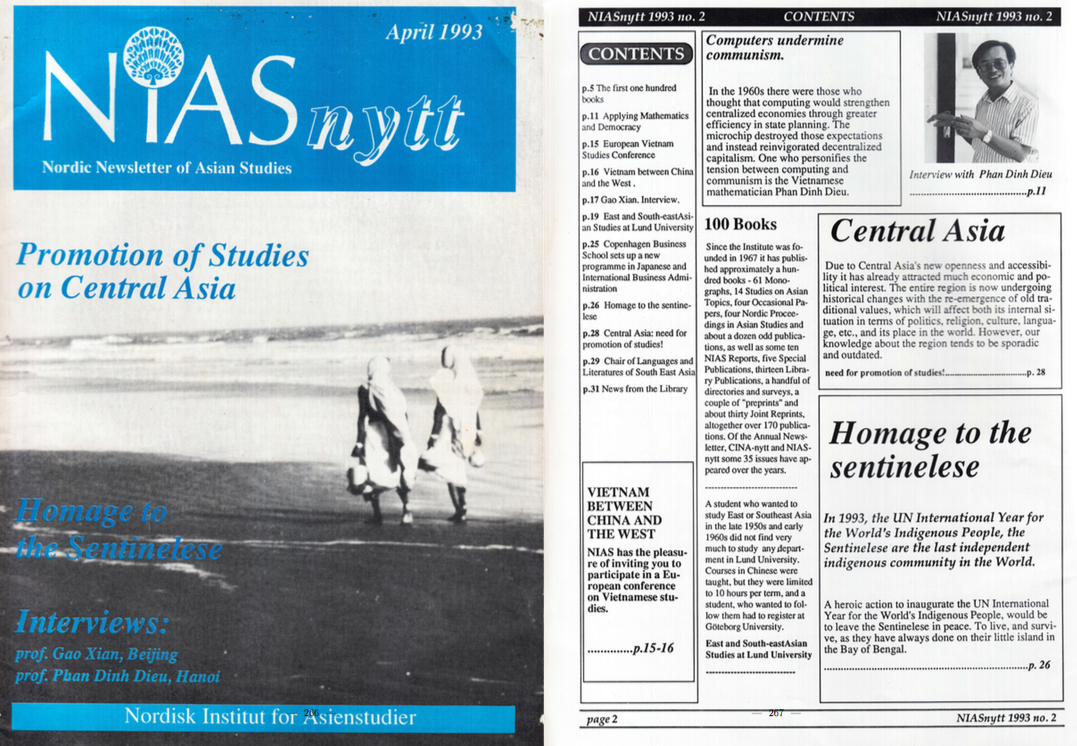
\includegraphics[scale=.3]{Nias}
\end{figure}
Computers undermine communism.


In the 1960s there were those who thought that computing would strengthen centralized economies through greater efficiency in state planning. The microchip destroyed those expectations and instead reinvigorated decentralized capitalism. One who personifies the tension between computing and communism is the Vietnamese mathematician Phan Dinh Dieu.


Interview with the Vietnamese mathematician Phan Dinh Dieu

\begin{center}
\textbf{Applying Mathematics and Democracy }
\end{center}


Computers undermine communism. In the 7960s there were those who thought that computing would strengthen centralized economies through greater efficiency in state planning. The microchip destroyed those expectations and instead reinvigorated decentralized capitalism. One who personifies the tension between computing and communism is the Vietnamese mathematician Phan Dinh Dieu. He is one of the few tolerated outspoken critics of party dictatorship inside Vietnam. Before the party congress in 7997, Dieu wrote a petition to the leadership pleading for democracy and suggesting that the party abandon Marxism-Leninism. The petition was not published, but was widely circulated. In September 1992 Dieu gave the following interview at his research institute in the suburbs of Hanoi.


\textbf{By Stein Tonnesson}


\noindent \textit{-	Professor Phan Dinh Dieu, in 1982 you published an article in Vietnamese Studies under the heading "Applying mathematics and computing". How come you are now trying to apply "democracy" as well? Is there any reason why a mathematician should be a politician?}


\noindent -	I am not a politician, but I want to participate in my country's decision-making as a ordinary citizen. I consider myself a patriot with a passion for poor people, and, therefore I want to contribute to my country's development. As a scientist I discovered quite some time ago that Marxism-Leninism had little to offer a country trying to overcome poverty. while studying computer science, systems theories and the problems of modern management I realized that the socialist model such as defined in Marxist-Leninist theory is unsuitable to a society wanting to develop socially, economically and scientifically. For obvious reasons Marx and Lenin did not have any means of understanding our modern society. But the communist parties both in Vietnam and elsewhere naively tried to apply Marxism- Leninism to the modern world. The failure of their attempt was demonstrated by the computer re-volution that characterized the world in the 1980s. The failure of the socialist economic system is now realized by virtually every-one. What remains is to draw the full conclusion and abandon Marxism- Leninism altogether.


\noindent \textit{-	It seems to me that in the economic field, the socialist model has already been abandoned in Vietnam.}


\noindent -	The main aspect of today's situation is the contradiction between the ambition to preserve the dictatorship of the party while at the same time developing a free market economy. This is a new combination. No communist theoretician has ever contemplated such a combination on anything like a permanent basis.


\noindent \textit{ -	Might not the current political system reflect an Asian, as opposed to a Western, concept of democracy?}


\noindent  -	There may be a difference in the current political realities of Asia and the West, but this does not have to do with different concepts of democracy. Democracy is democracy wherever it is applied. The first requirement of a, democratic system is respect for human rights and the rights of the citizen. That applies everywhere. And the rights of the citizen must be respected by the holding of free elections. The key element in democratic system is the way that leaders are elected. Democratic elections are free, with a secret ballot, ffid with the right for everyone to stand as candidates. If these requirements are not met, there is no democracy.  Let me add that of course there can be various degrees of democracy. It is not perfect anywhere, not even I suppose in your country, or in Germany, France, the United States. The quality of a democracy can be measured on two accounts. The first is the way that the electoral system functions; does it provide for real choices, and to what extent do the results of the elections reflect public opinion? The second is the opportunity and capacity that people have to influence actual decision-making through discussions in the media, meetings etc., both on the local, regional and national level.


\noindent -	\textit{Does this mean that you favour a multi-party, system in Vietnam?}


\noindent -	The essential thing is not to have many parties or a "multi-party system", but to have a real choice. To have a real choice, two parties may be enough, but then there must be a real difference between them.


\noindent -	\textit{Don't you fear that the introduction of opposition parties might endanger the current social stability and economic growth in Vietnam, perhaps even lead to chaos?}


\noindent -	Yes, I realize that there is such a danger; that's why I said two parties might be enough. One basic mathematical theorem says that a signed graph is in balance if and only if it is bipartite. If there are many parties, a political system risks to become chaotic unless the parties combine forces around two poles. The two-party systems of the United States and Great Britain have been more stable than some multi-party systems, for instance the French system after the Second World War. But the current political system in Vietnam is a unipolar system. As long as it can keep down all opposition, it is stable, but a dynamic stability with a positive development can only be achieved by accepting the introduction of an opposite pole. Please note that an ‘opposite’ pole does not mean destructive, but constructive.


\noindent -	\textit{The current Vietnamese leader seem to have gone a long way towards accepting the freedoms of opinion and expression.}


\noindent -	The dictatorship of the party is no longer as fundamental as it used to be. There was a time when even our food rations were decided on the basis of our loyalty to the party. Now there is a lot more freedom, but in my view the years 1987 and 1988 were freer than the years since. At that time we experienced the beginning of a political and theoretical debate which was aborted by later developments.


\noindent -	\textit{Journalists are stilt encouraged to unveil and criticize corruption and abuse of power.}


\noindent -	This is true, but there are clear limits. The main prohibition concerns criticism of the dictatorship of the party. The party cannot be criticized as such on any level, not even the district level. Corruption can be allowed to be criticized since it is not a problem proper to our political system. It is a global problem. Corruption basically means to "sell power". Power is sold in most, perhaps all, countries, but of course to a different extent. The current state of affairs in Vietnam enhances corruption. In a centralized communist society, corruption is deflected by the lack of a market. The benefits of power come from institutionalized privileges rather than from the selling of power. In democratic societies corruption is to some extent precluded by the lack of discretion or secrecy; the fear of being exposed or indicted reduces the temptation to sell power. In today's Vietnam we have the worst of both worlds: a flourishing market where power can be sold, and yet a very high degree of discretion and secrecy within the ruling elite. When some of us asked that the names be released of those officials who had obtained houses for free Ho Chi Minh by virtue of their public positions and then sold them on the market, we were not heard. That political system does not allow full exposure of corruption when it happens on such an important level. 


\noindent -	\textit{Let me return to the question of democracy: Do you think that the ‘other pole’ can develop within the current National Assembly?}


\noindent -	I have little faith in the new National Assembly [elected in July 1992]. The election consisted in a choice between a few candidates who had been handpicked by the party and the Fatherland Front. There were some 40 who tried to pose as "independents", but only two of them were accepted as candidates, and they were not elected. The level of education of the Assembly members is much higher than before, but I see no one in the Assembly who can play an independent role. Discussion will be within the confines set by the party.


\noindent -	\textit{Where then do you see hope? Among the intellectuals? During the last party congress, the role of intellectuals in Vietnam was heavily upgraded.}


\noindent -	Before speculating about a possible role for the intellectuals, I would like to ask: Who are our intellectuals? Do we really have an intelligentsia in Vietnam, an independent social and political intellectual force? This is an important question to be asked of all societies that inspire to introduce or improve upon democracy.
Let me first mention the group of patriotic intellectuals who were educated in the French period. Among them there are many respectable and courageous personalities. Some of them are still with us, but they no longer wield much influence. In fact, there are very few left. We should cherish them for what they have done for the nation. 
Secondly, there is a very large number of specialists educated during the socialist period. In contrast to the French regime, the socialist regime educated specialists rather than intellectuals. 'We have a great many mathematicians, physicists, biologists, engineers etc., and are now having more and more economists. But they were never taught to think about society. The party was to do the thinking for everyone. The political awareness of the specialists is generally weak. The best of them participate in government and, quite naturally, belong to the party. It is possible that many specialists harbour democratic ideas privately, but we don't really have any means of knowing if such is
the case.
Thirdly, there are the intellectuals of the former South Vietnam. Most of them have left the country. They may of course come back and serve the nation in various ways, but to play a significant political role, intellectuals must be in close contact with people. A protracted exile is no good background for a positive intellectual force. 
Lastly, there are the young, those who were only recently educated or are now under education, and whose formative years have been characterized by Doi Moi ["Doi Moi" is the Vietnamese equivalent to "perestroika"]. These last years, we have had a reinvigoration of independent art and literature. But there still is a long way to go before these tendencies may coalesce into a real political and social force. 
All in all, I have to conclude that rye lack an intellectual class.


\noindent -	\textit{Does this mean you ore generally pessimistic, or do you see hope somewhere?}


\noindent -	It may surprise you after what I said about the dictatorship of the party, but I persist in hoping that the party itself will change. People who think responsibly about our country's future must favour change with stability. The best way to achieve this is to convince the party that it should face realities and abandon its old ways. I have written petitions and I have talked to the party leaders, and at least they have listened. You see, the party has two sides, the communist side and the patriotic side. If it could keep the latter and abandon the former, it might transform itself into a genuinely patriotic force. Some of our top leaders, to my knowledge, are very sincere men.


\noindent -	\textit{But how then would You get your second "pole"?}


\noindent -	That will be the real test of the responsibility and courage of the leadership. If they are to be real patriots they must accept the transformation of the party into a patriotic party with full respect for the basic freedoms and they must introduce free elections. And under such conditions other political organizations will appear which will gradually develop into a constructive opposition. If the party transforms itself along such lines, it may win all elections for a long period ahead.


\noindent -	\textit{And do you see a role for yourself in this transformation? Are you Vietnam's Sacharov?}


\noindent -	As I said, I am not a politician, and I have no ambitions. But as a scientist and a, patriotic citizen, I want to participate. Democracy requires participation.


\newpage

Bản đánh máy có thể đọc tại \url{http://hieuminh.org/2012/02/02/interview-with-the-vietnamese-mathematician-phan-dinh-dieu/}\\
 \\
\\

\noindent  \textbf{Stein TØNNESSON (ST)}: Năm 1982, ông công bố trên tạp chí Nghiên cứu Việt Nam một bài báo nhan đề “ ứng dụng toán học và máy tính điện tử”. Nay dường như ông muốn ứng dụng toán học vào cả vấn đề dân chủ. Vì sao một nhà toán học lại trở thành chính khách ?\\
\textbf{Phan Đình Diệu (PĐD)}: Tôi không phải là chính khách, mà tôi chỉ muốn tham gia vào việc nước như một công dân. Là một người yêu nước, thiết tha với nhân dân nghèo khó, tôi muốn đóng góp vào công cuộc phát triển đất nước. Là một người làm khoa học, đã từ khá lâu tôi phát hiện ra rằng chủ nghĩa Mác-Lê khó có thể mang lại điều gì hữu ích cho một nước muốn thoát ra khỏi nghèo nàn. Nghiên cứu khoa học điện toán, thuyết hệ thống và các vấn đề quản lý hiện đại, tôi nhận ra rằng mô hình xã hội chủ nghĩa như học thuyết Mác-Lê xác định không phù hợp với một nước muốn phát triển về xã hội, kinh tế và khoa học.Vì những lý do hiển nhiên, Marx và Lenin không có điều kiện tìm hiểu xã hội hiện đại. Song đảng cộng sản ở Việt Nam cũng như ở các nước khác đã ngây thơ tìm cách áp dụng học thuyết của họ vào xã hội hiện đại. Sự thất bại của họ đã được minh chứng rõ rệt nhất trong cuộc cách mạng điện toán, đặc trưng của thế giới trong thập niên 1980. Sự thất bại của hệ thống kinh tế xã hội chủ nghĩa ngày nay hầu như mọi người đều thấy rõ. Vấn đề còn lại là biết rút ra kết luận một cách đầy đủ và từ bỏ chủ nghĩa Mác-Lê\\
\textbf{ST}: Tôi có cảm tưởng là trong lãnh vực kinh tế, thực ra Việt Nam đã từ bỏ mô hình xã hội chủ nghĩa rồi.\\
\textbf{PĐD}: Nét nổi bật trong tình hình hiện nay là sự mâu thuẫn giữa một mặt là ý muốn duy trì sự chuyên chế của đảng, và mặt khác, phát triển thị trường tự do. Đây là là một sự kết hợp mới. Chưa hề có một nhà lý luận cộng sản nào nghiên cứu tình thế này trên một cơ sở có thể coi là thường trực.\\
\textbf{ST}: Phải chăng hệ thống chính trị hiện nay phản ánh một quan niệm Á châu về dân chủ, khác với quan niệm dân chủ Tây phương?\\
\textbf{PĐD}: Có thể có sự khác biệt về thực tế chính trị giữa châu Á và phương Tây, chứ không có quan niệm khác nhau về dân chủ. Dân chủ thì ở đâu cũng là dân chủ. Một hệ thống dân chủ đòi hỏi trước hết phải tôn trọng các quyền con người và quyền công dân. Điều này đặt ra ở mọi nơi. Và quyền công dân phải được tôn trọng bằng cách tổ chức bầu cử tự do. Nhân tố then chốt của một chế độ dân chủ là cách bầu ra người lãnh đạo. Bầu cử dân chủ nghĩa là bầu cử tự do, bỏ phiếu kín, và mọi người đều có quyền ra ứng cử. Không có những điều đó, không thể gọi là dân chủ. Cũng cần nói thêm: tất nhiên có những mức độ khác nhau về dân chủ. Theo tôi nghĩ, không có nơi nào nền dân chủ có thể coi là hoàn thiện, kể cả ở nước ông [tức là Na Uy, chú thích của người dịch], hay ở Đức, Pháp hoặc Hoa Kỳ. Chất lượng một chế độ dân chủ có thể đo bằng hai tiêu chuẩn. Thứ nhất là cách vận hành của thể chế bầu cử: cử tri có thực sự được chọn lựa hay không, kết quả cuộc bầu cử phản ánh dân ý tới đâu? Thứ nhì là khả năng của nhân dân tác động vào quá trình quyết định thông qua thảo luận trên các media, trong các cuộc hội họp, gặp gỡ ở địa phương, cũng như ở cấp vùng, và cấp toàn quốc.\\
\textbf{ST}: Phải chăng ông chủ trương thiết lập một chế độ đa đảng ở Việt Nam?\\
\textbf{PĐD}: Điều cốt yếu không phải là có nhiều đảng, không phải là có một chế độ đa đảng, mà là có sự chọn lựa thật sự. Muốn chọn lựa thật sự, hai đảng có thể cũng đủ, với điều kiện là hai đảng ấy thực sự khác nhau.\\
\textbf{ST}: Ông có ngại rằng đặt ra những đảng đối lập có thể tác hại tới sự ổn định xã hội và sự tăng trưởng kinh tế hiện nay ở Việt Nam, thậm chí gây ra hỗn loạn chăng?\\
\textbf{PĐD}: Vâng, tôi nghĩ có nguy cơ đó; bởi vậy tôi mới nói hai đảng cũng đủ. Trong toán học có một định lý cơ bản: một biểu đồ định hướng là cân bằng nếu như và chỉ nếu như nó có hai nhánh (tiếng Anh bipartite còn có nghĩa là hai bên, hai đảng). Nhiều đảng quá có thể dẫn tới hỗn loạn – trừ phi các đảng liên kết chung quanh hai cực. Hệ thống lưỡng đảng ở Hoa Kỳ hay ở Vương quốc Anh xem ra ổn định hơn là hệ thống nhiều đảng như ở Pháp dưới thời đệ tứ cộng hoà. Còn ở Việt Nam hiện nay là hệ thống chính trị độc đảng. Ngày nào chế độ còn trấn áp được mọi sự đối lập thì hệ thống còn ổn định, nhưng đó chỉ là một sự ổn định tĩnh. Còn sự ổn định động, hàm ý phát triển tích cực, chỉ có thể thực hiện bằng cách lập ra một “đối cực”. Xin hiểu đối cực theo nghĩa xây dựng của nó, chứ không phải phá hoại.\\
\textbf{ST}: Các nhà lãnh đạo hiện nay của Việt Nam dường như đã tiến một bước khá dài trong việc thừa nhận quyền tự do ý kiến và tự do phát biểu.\\
\textbf{PĐD}: Sự chuyên chế của đảng không còn toàn diện như trước kia. Có một thời, ngay cả khẩu phần lương thực cũng được quyết định trên cơ sở lòng trung thành đối với đảng. Bây giờ đã tự do hơn, nhưng theo ý tôi, 1987 và 1988 là những năm tự do hơn là từ đó đến nay. Trong hai năm ấy, chúng tôi đã bước đầu thể nghiệm thảo luận về chính trị và lý luận, sau đó bị dẹp.\\
\textbf{ST}: Người ta vẫn khuyến khích báo chí tố cáo tham nhũng, lạm quyền.\\
\textbf{PĐD}: Đúng thế, nhưng với những hạn chế rất rõ ràng. Điều cấm kỵ chủ yếu liên quan tới sự chuyên chế của đảng. Không ai được quyền phê bình đảng, cho dù ở cấp huyện. Tham nhũng thì được phép phê phán, vì tham nhũng không phải là vấn đề hệ thống chính trị. Đó là một vấn đề chung. Tham nhũng chung quy có nghĩa là bán quyền lực. Có lẽ ở đâu cũng có sự bán quyền lực, khác nhau là ở quy mô. Tình hình làm ăn hiện nay ở Việt Nam đang làm cho tham nhũng phát triển. Trong một xã hội cộng sản tập trung, sự tham nhũng chừng nào bị lệch dòng (deflected) vì thiếu vắng thị trường. Các đặc lợi phát sinh từ các đặc quyền hơn là do buôn bán quyền thế. Trong những xã hội dân chủ, do không giữ được (hoặc ít giữ được) bí mật, nên ở chừng mực nào đó, sự tham nhũng bị ngăn chặn, hay hạn chế; người ta không (hoặc ít) dám buôn bán quyền lực vì sợ bị tố cáo hoặc truy tố. Còn ở Việt Nam hiện nay, chúng tôi gặp cả hai cái nạn ấy cộng lại: một thị trường mặc sức phát triển trong đó quyền lực là một thứ hàng hoá buôn đi bán lại, song song tồn tại với một giới cầm quyền giữ bí mật cao độ. Vừa qua có vụ hoá giá nhà ở thành phố Hồ Chí Minh, cán bộ cấp cao được mua nhà công với giá rẻ, và bán lại với giá thật cao, chúng tôi đòi công bố danh sách, song người ta lờ đi. Hệ thống chính trị này không cho phép công bố đầy đủ thông tin về tham nhũng trong những vụ việc có quy mô quá lớn như vậy.\\
\textbf{ST}: Tôi muốn trở lại vấn đề dân chủ: ông có cho rằng “ đối cực”, hay ít nhất, là cái cực kia, có thể phát triển ngay trong quốc hội hiện nay không?\\
\textbf{PĐD}: Tôi không mấy tin tưởng vào Quốc hội mới được bầu [tháng 7.1992]. Cuộc bầu cử quốc hội vừa rồi là chọn giữa vài ứng cử viên đã được đảng và Mặt trận Tổ quốc lựa ra từ trước. Khoảng 40 người ra ứng cử độc lập, nhưng người ta chỉ chấp nhận cho 2 người ứng cử, và cả hai đều thất cử. Trình độ học vấn của các đại biểu khoá này cao hơn khoá trước, nhưng tôi không thấy ai có thể đóng một vai trò độc lập. Các cuộc thảo luận ở Quốc hội vẫn diễn ra trong lằn ranh do đảng vạch ra.\\
\textbf{ST}: Thế thì ông đặt hy vọng vào đâu? Vào giới trí thức? Trong đại hội Đảng vừa qua, vai trò của trí thức đã được nâng cấp một cách đáng kể?\\
\textbf{PĐD}: Trước khi bàn về vai trò trí thức, thử hỏi: trí thức là ai? Ở Việt Nam có hay không có một giới trí thức, một lực lượng trí thức độc lập về xã hội và chính trị? Đó là vấn đề quan trọng đặt ra cho mọi xã hội muốn thiết lập hay cải thiện chế độ dân chủ. Trước tiên, tôi muốn nói tới lớp những nhà trí thức đã được đào tạo dưới thời Pháp thuộc. Trong lớp này, có những nhân vật dũng cảm và đáng kính. Một vài vị còn sống nhưng không còn mấy ảnh hưởng. Thật ra, chỉ còn lại một số rất nhỏ. Chúng tôi quý trọng công lao của họ đối với dân tộc. Lớp thứ hai là một số đông những chuyên gia được đào tạo trong giai đoạn xã hội chủ nghĩa. Trái ngược với nền giáo dục thời Pháp, chế độ xã hội chủ nghĩa đào tạo ra những chuyên viên hơn là những trí thức. Chúng tôi có nhiều nhà toán học, nhà vật lý học, nhà sinh học, kỹ sư... và bây giờ thêm nhiều nhà kinh tế. Nhưng chưa bao giờ họ được học để suy nghĩ về các vấn đề của xã hội. Đảng nghĩ hộ cho mọi người. Ý thức chính trị của các chuyên viên nói chung là yếu. Những người giỏi tham gia chính quyền, và tự nhiên là đảng viên. Rất có thể nhiều chuyên viên, trong cuộc sống riêng, cũng có tư tưởng dân chủ, nhưng không có cách gì kiểm nghiệm điều đó cả. Thành phần thứ ba là những trí thức được đào tạo trước đây ở miền Nam. Phần đông đã bỏ đi. Tất nhiên có thể họ sẽ trở về giúp nước bằng cách này hay cách khác, nhưng muốn đóng một vai trò chính trị có ý nghĩa, thì người trí thức phải gần gụi nhân dân. Cuộc sống kéo dài ở hải ngoại không phải là mảnh đất thuận lợi cho một lực lượng trí thức tích cực. Cuối cùng là thanh niên, những người vừa được hay còn đang được đào tạo trong những năm gọi là đổi mới. Những năm gần đây, quả đã có một nền văn nghệ độc lập khởi sắc. Nhưng còn phải có thời gian thì các xu hướng nói trên mới có thể hình thành một lực lượng xã hội chính trị thực sự. Nói tóm lại, kết luận của tôi là hiện nay Việt Nam chưa có một giai cấp trí thức.\\
\textbf{ST}: Nghĩa là nhìn về toàn cục thì ông bi quan? Hay ông còn thấy có hy vọng ở đâu đó?\\
\textbf{PĐD}: Tôi nói điều này chắc ông ngạc nhiên: mặc dầu tôi đã nói như ở trên về sự chuyên chế của đảng cộng sản, song tôi vẫn hy vọng là đảng cộng sản tự nó sẽ thay đổi. Những ai suy nghĩ một cách có trách nhiệm về tiền đồ dân tộc tất phải tán thành sự thay đổi trong ổn định. Cách tốt nhất để thực hiện việc này là thuyết phục đảng cộng sản phải biết nhìn nhận thực tế và từ bỏ con đường cũ. Tôi đã soạn những bản kiến nghị và nói với những nhà lãnh đạo đảng. Ít nhất họ đã nghe tôi nói. Theo tôi, đảng cộng sản Việt Nam có hai mặt, mặt cộng sản và mặt yêu nước. Nó nên giữ mặt thứ nhì và bỏ mặt thứ nhất, nó có thể tự biến đổi thành một lực lượng yêu nước chân chính. Theo chỗ tôi biết, có những nhà lãnh đạo cấp cao là những người rất chân thành.\\
\textbf{ST}: Nhưng làm thế nào đi tới cái thế lưỡng cực?\\
\textbf{PĐD}: Đây chính là sự thử thách lớn về tinh thần trách nhiệm và sự dũng cảm của giới lãnh đạo. Nếu họ thực sự yêu nước thương dân thì họ phải chấp nhận biến đảng trở thành một đảng dân tộc, tôn trọng đầy đủ các quyền tự do cơ bản và tổ chức bầu cử tự do. Trong điều kiện đó, những tổ chức chính trị khác sẽ xuất hiện, từng bước triển khai thành một lực lượng đối lập xây dựng. Nếu đảng cộng sản tự cải tạo trong quá trình đó, thì trong suốt một thời gian dài, nó có thể thắng cử.\\
\textbf{ST}: Ông có nghĩ rằng ông có thể đóng một vai trò trong tiến trình biến đổi đó hay không? Phan Đình Diệu phải chăng là Sakharov của Việt Nam?\\
\textbf{PĐD}: Như tôi đã nói ở trên, tôi không phải là một chính khách và tôi không có tham vọng (chính trị). Song, với tư cách một nhà khoa học và một công dân yêu nước, tôi muốn tham gia việc nước. Dân chủ là tham gia việc nước.
%Stein TØNNESSON


  %\includepdf[pages=1-,noautoscale,pagecommand={\thispagestyle{plain}}]{Docs/1993_04_Nordic_Newsletter.pdf}

\chapter{Báo Far Easrten Economic Review 02/1993}\index{Báo chí}

%\clearpage{\pagestyle{empty}\cleardoublepage}
  %\includepdf[pages=1-,noautoscale,pagecommand={\thispagestyle{plain}}]{Docs/1993_02_VietnamesedissidentAndMathematicien.pdf}
  
\begin{center}
    \begin{figure}[htp]
    \begin{center}
     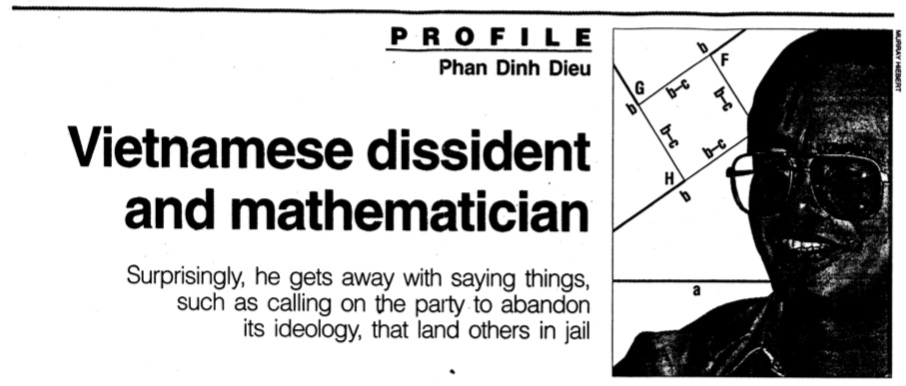
\includegraphics[scale=.3]{9302}
    \end{center}
   
    \label{refhinh1}
    \end{figure}
\end{center}

\begin{flushright}
PROFILE \\
Phan Dinh Dieu
\end{flushright}

\textbf{\Large Vietnamese dissident and mathematican.} 

\textit{Surprisingly, he gets away with saying things such as calling on the party to abandon its ideology, that land others in jail. }

\textbf{By Murray Hiebert}


Phan Dinh Dieu gets away with saying things few other Vietnamese dare utter in public. The 56-year-old mathematician calls on the ruling communist party to abandon its Marxist-Leninist ideology and challenges it to allow other parties to compete in the country’s political life.


Dieu believes Vietnam remains in a deep state of crisis, despite the party's six- year reform programme. He charges that abuse of power, corruption and smuggling are increasing while health care, education and living standards generally continue to deteriorate. He is convinced the only way out of this crisis is for the party to- introduce wide-ranging political reforms.


"Some people think democracy is a luxury for a poor country like Vietnam and say we need more food, not more democracy," Dieu says. “But to have more food and clothes, one must have more democracy. Without a democratic system, you have a dictatorship, social diseases in society can't be avoided and the efficient development of a market economy can’t be realised ."


"Democracy demands pluralism, a multi-party system," the mathematician adds. "Democracy means everyone must have the right to express what he thinks. In a democracy, you must have different political forces and organisations guaranteeing the rights of the people."


Some intellectuals who have made similar demands, such as the writer Duong Thu Huong and the physician Nguyen Dan Que, have-ended up in jail. Other professors have been squeezed out of their university jobs or had their requests to travel abroad rejected.


Dieu not only stays out of prison and retains his post as vice-chairman of Viet-nam's National Centre for Scientific Research but he continues to get permission to travel abroad, to France, the US and ]apan. He is even invited to talk with Vietnamese leaders about his political views.


In September 1991, he met with then newly elected party chief Do Muoi to discuss a 10-page petition Dieu had circulated prior to the party’s seventh congress in |June. More recently, he has participated in discussions about the crisis facing world communism at the Institute of Social Sciences, the Marxist-Leninist Institute in Hanoi and the Nguyen Ai Quoc Institute in Danang, where many of the party’s leading cadres are trained.


\begin{center}
\textbf{‘SOME PEOPLE SAY DEMOCRACY IS A LUXURY FOR A POOR COUNTRY LIKE VIETNAM’ }
\end{center}

Dieu was born in Ha Tinh, one of Viet-nam's poorest provinces and the birth place of the late Ho Chi Minh. In 1954, the year Ho's troops defeated French colonial forces at Dien Bien Phu, Dieu entered Hanoi University. Eight years later, he was granted a scholarship to study mathematics in the former Soviet Union.


He returned to Vietnam in 1967 and began working in the Science Committee's Mathematics Institute. His wife, now retired, worked in the same institute. They' have three children. The oldest daughter is studying in an economic institute in France. A second daughter is studying mathematics at Hanoi University. The third child, a son, is in the eighth grade.


Dieu was twice elected as a representative to the National Assembly between 1976 and 1981 but he says the party did not nominate him again after he made repeated calls for greater democracy. 


Much of Dieu's research has focused on computer science since he was appointed director of the Computer Science-Institute in 1977. Today he is working on two major research projects: one focuses on artificial intelligence and the other on protecting information in computer databases.


But Dieu is more admired among intellectuals in Vietnam for his daring political critiques than for his scientific research. Many observers are uncertain why Dieu's pummeling of the party is tolerated, while the voices of most of the party’s other strident opponents are silenced.


Some of Dieu's most cynical critics say, the mathematician has been invited by the party to play the role of  "token" dissident. He sharply rejects the charge. "Nobody in power has asked me to do this or that", he says. 'What I do I do only following my conscience, my responsibility before our poor country."


Dieu believes Vietnam's party is more popular than the former communist parties in Eastern Europe because of its role in fighting for independence and national reunification against the French and the Americans. 'Our party had very big success when it remained a party of patriotism," he says. "It failed when it became communist."


Dieu lists among the party’s biggest mistakes the land reform programme in the 1950s, when thousands of landlords were killed, and the shutting down of capitalist enterprises in the south in 1978. "We must recognise that the theories of communism and socialism have brought our country many privations: a nation divided and paralysed, a devastated economy, an impoverished and backward livelihood [and] isolation from the civilized  world," he wrote in his 1991petition to the party.


Dieu says the reform progranune has brought a 'better face" to the economy, but resulted in few political changes. What I propose," he explains, "is not an end to the leadership role of the party, but an end to the dictatorship of the party. If the party gets a majority in free and democratic elections, then I will support it."$\blacksquare$

\begin{center}
FAR EASTERN ECONOMIC REVIEW 			11 FEBRUARY 1993
\end{center}

\newpage
 
\begin{flushright}
Về ông Phan Đình Diệu
\end{flushright}

\begin{center}
\textbf{Nhà bất đồng chính kiến và nhà toán học người Việt.}
\end{center}


\textit{Thật bất ngờ, ông đã không vấn đề gì sau những phát ngôn kêu gọi Đảng cộng sản Việt nam nên từ bỏ ý thức hệ của mình vì ý thức hệ đó đẩy nhiều người vào cảnh tù đày. }


\textbf{By Murray Hiebert}


Giáo sư Phan Đình Diệu không gặp vấn đề gì cho dù ông đã phát ngôn những vấn đề mà chỉ rất ít người Việt dám bày tỏ công khai. Nhà toán học 56 ​​tuổi kêu gọi Đảng cộng sản cầm quyền hãy từ bỏ ý thức hệ Marxist-Leninist và hãy để cho các đảng phải khác cùng cạnh tranh với nhau trong đời sống chính trị tại đất nước Việt Nam. 


Ông cho rằng Việt Nam vẫn đang trong tình trạng khủng hoảng sâu sắc cho dù Đảng đã có một chương trình tái cấu trúc dài sáu năm. Ông cáo buộc việc lạm dụng quyền lực, tham nhũng và buôn lậu đang gia tăng trong khi những vấn đề về chăm sóc sức khoẻ, giáo dục và mức sống của người dân đang có chiều hướng ngày càng tồi tệ. Ông tin rằng cách duy nhất thoát khỏi cuộc khủng hoảng này chính là Đảng cộng sản phải công bố các cuộc cải cách chính trị toàn diện trong nội bộ Đảng.



Ông cho biết: "Một số người cho rằng dân chủ là một thứ xa xỉ đối với nước nghèo như Việt Nam và họ nói rằng tôi cần cơm ăn áo mặc nhiều hơn là cần dân chủ. Nhưng để có thêm cơm ăn áo mặc thì phải dân chủ hơn. Khi chưa có một hệ thống dân chủ, vẫn tồn tại chế độ độc tài thì các bệnh dịch trong xã hội không thể tránh được và không thể phát triển một cách thật hiệu quả nền kinh tế thị trường”.  


Ông bổ sung: "Dân chủ đòi hỏi phải đa nguyên, đa đảng. Dân chủ có nghĩa là mọi người đều có quyền bày tỏ suy nghĩ của mình. Trong một nền dân chủ, phải có những lực lượng chính trí khác nhau cùng với các tổ chức nhằm đảm bảo quyền lợi của người dân”. 


Nhiều nhà trí thức cũng đã từng có những đòi hỏi tương tự như nhà văn Dương Thu Hương, bác sĩ Nguyễn Đan Quế - người đã bị bắt giam. Một số giáo sư khác cũng đã bị buộc phải ra khỏi các trường đại học mình đang công tác hoặc mọi đề nghị được đi ra nước ngoài của họ đều bị từ chối. 


Ông Diệu không những không phải chịu cảnh tù đày mà còn được giao giữ những chức vụ quan trọng như phó Chủ tịch Trung tâm Nghiên cứu Khoa học Quốc gia và có quyền được đi ra nước ngoài như tới Pháp, Mỹ và Nhật. Ông còn được mời nói chuyện với các nhà lãnh đạo Việt Nam về quan điểm chính trị cá nhân ông.  


Tháng 9/1991, ông Diệu có cuộc gặp gỡ với ông Đỗ Mười – người mà sau này đã được bầu làm Tổng Bí Thư Đảng Cộng sản, trong cuộc gặp đó ông Diệu đã trao đổi một bản kiến nghị dày 10 trang mà ông đã từng công bố rộng rãi trước khi Đại hội VII diễn ra hồi tháng 6. Gần đây nhất, ông Diệu đã tham gia các cuộc thảo luận về cuộc khủng hoảng mà chủ nghĩa cộng sản toàn cầu đang phải đối mặt tại Viện Khoa học Xã hội, Viện Triết học Mác - Lênin tại Hà Nội và Học viện Nguyễn Ái Quốc ở Đà Nẵng – nơi đang đào tạo nhiều cán bộ nguồn cho Đảng cộng sản. 


\begin{center}
\textbf{'NHIỀU NGƯỜI CHO RẰNG DÂN CHỦ LÀ MỘT THỨ XA XỈ ĐỐI VỚI QUỐC GIA NGHÈO NHƯ VIỆT NAM”. }
\end{center}

Giáo sư Diệu sinh ra tại Hà Tĩnh, một trong những tỉnh nghèo nhất của Việt Nam và cũng là nơi sinh của Chủ tịch Hồ Chí Minh. Năm 1954, quân đội của ông Hồ Chí Minh đã đánh bại lực lượng quân đội viễn chinh Pháp tại Điện Biên Phủ, khi đó ông Diệu mới đặt chân vào trường Đại học ở Hà Nội. Tám năm sau, ông giành được học bổng theo học ngành Toán tại Liên Xô cũ.  


Năm 1967, Ông trở về Việt Nam và bắt đầu làm việc tại Viện Toán học của Uỷ ban Khoa học. Vợ ông (đã nghỉ hưu) làm cùng tại Viện Toán. Họ có ba người con: con gái đầu đang theo học tại Viện kinh tế ở Pháp, con gái thứ hai đang học toán bậc Đại học ở Hà Nội, còn con trai thứ ba đang học lớp 8. 


Giáo sư Diệu từng hai lần được bầu làm đại biểu Quốc hội từ năm 1976 đến năm 1981 nhưng ông cũng cho biết Đảng cộng sản Việt Nam đã không giới thiệu ông nhiệm kỳ kế tiếp sau khi ông nhắc lại lời kêu gọi cần phải dân chủ hơn nữa.  
Kể từ khi được bổ nhiệm làm Giám đốc Viện Khoa học Máy tính năm 1977, hầu hết các nghiên cứu của Giáo sư Diệu đều tập trung vào ngành khoa học máy tính. Hiện ông đang làm về hai mảng dự án nghiên cứu: trí tuệ nhân tạo và bảo vệ thông tin trong dữ liệu máy tính.


Thực tế thì Giáo sư Diệu được giới trí thức Việt Nam ngưỡng mộ nhiều vì ông dám lên tiếng phản biện chính trị hơn là những nghiên cứu khoa học của ông. Nhiều nhà quan sát vẫn chưa dám khẳng định tại sao việc lên tiếng của ông về Đảng cộng sản lại không hề hấn gì trong khi rất nhiều tiếng nói khác về Đảng cộng sản của những người đối lập khác đều rơi vào im lặng.


Một số nhà phê bình hoài nghi nhất đã từng nói nhà toán học được Đảng cộng sản mời để giữ vị trí đối lập “bù nhìn”. Ông Diệu đã phản bác lại lời cáo buộc trên với lập luận: “Không ai có quyền yêu cầu tôi phải thực hiện một việc hoặc không thực hiện việc đó. Điều tôi làm là lương tâm tôi mách bảo, đó là trách nhiệm cá nhân tôi trước dân tộc nghèo đói của tôi”.  


Ông cho rằng Đảng cộng sản ở Việt Nam phổ biến hơn các đảng cộng sản ở Đông Âu vì vai trò của nó trong cuộc đấu tranh giành độc lập và thống nhất đất nước trước các cuộc xâm lược của Pháp và Mỹ. Ông nói: "Đảng cộng sản đã rất thành công khi đó là Đảng yêu nước và nó đã thất bại khi nó trở thành Chủ nghĩa Cộng sản”. 


Ông đã chỉ ra những sai lầm lớn nhất của Đảng cộng sản trong cuộc cải cách ruộng đất những năm 1950, khi đó hàng ngàn địa chủ bị giết, hàng loạt doanh nghiệp tư bản ở miền Nam năm 1978 buộc phải đóng cửa. Trong bản kiến nghị năm 1991 gửi tới Đảng Cộng Sản ông viết: "Chúng ta phải thừa nhận rằng các lý thuyết về chủ nghĩa cộng sản và chủ nghĩa xã hội đã đưa đất nước đến nhiều hệ lụy: quốc gia bị chia rẽ và tê liệt, kinh tế đình trệ, đời sống khó khăn, lạc hậu và tách khỏi thế giới văn minh”. 


Giáo sư Diệu nói công cuộc đổi mới đã mang lại một diện mạo mới đối với nền kinh tế nhưng đã dẫn đến thay đổi chính trị ít nhiều. Ông giải thích thêm: “Những gì tôi đề xuất không phải là chấm dứt vai trò lãnh đạo của Đảng mà là chấm dứt chế độ độc tài Đảng trị. Nếu Đảng mà chiếm được đa số phiếu bầu trong một cuộc tranh cử dân chủ và tự do thì cái đó tôi hoàn toàn ủng hộ”.


\begin{center}
TẠP CHÍ KINH TẾ VIỄN ĐÔNG 			NGÀY 11 THÁNG 2 NĂM 1993
\end{center}





\chapter{Báo Far Easrten Economic Review 08/1993}\index{Báo chí}

%\clearpage{\pagestyle{empty}\cleardoublepage}
  %\includepdf[pages=1-,noautoscale,pagecommand={\thispagestyle{plain}}]{Docs/1993_08_FarEasrtenEconomicReview.pdf}
\begin{figure}
\centering
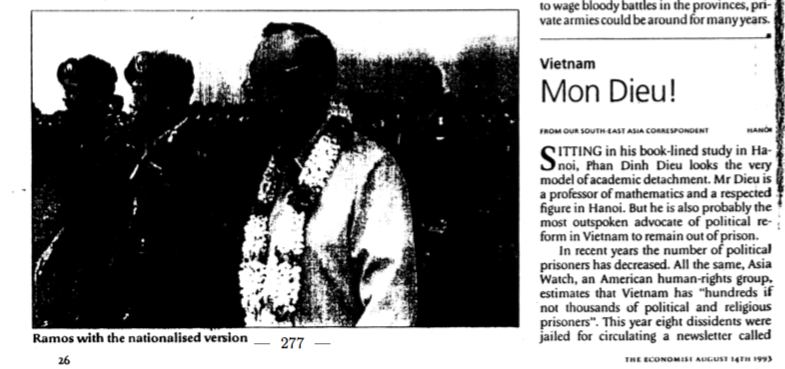
\includegraphics[scale=.4]{FE2}
\end{figure}  
  
  
\textbf{INTELLIGENCE}\\
\textbf{Adieu Dr Dieu}


Vietnamese mathematician, long the most outspoken critic of the ruling Communist Party to remain out of prison, has been ousted from his post as vice-chairman of the National Centre for Scientific Research. In recent months, Dieu had called for the party to abandon its Marxist-Leninist ideology and challenged it to allow other parties to compete in the country’s political life. Officially, he was removed from his post in a dispute with the centre’s director physicist Nguyen Van Hieu, but observers see Dieu’s firing as an attempt by the party to isolate him from potential supporters, Dieu has asked to be allowed to teach mathematics and computer science at Hanoi University. 




\textbf{VIETNAM}\\

 Mon Dieu!


\textbf{FROM OUT SOUTH-EAST ASIA CORRESPONDENT    \quad           HANOI}


Sitting in his book-lined study in Hanoi, Phan Dinh Dieu looks the very model of academic detachment. Mr Dieu is a professor of mathematics and a respected figure in Hanoi. But he is also probably the most outspoken advocate of political reform in Vietnam to remain out of prison. 


In recent years the number of political prisoners has decreased. All the same, Asia Watch, an American human-rights group, estimates that Vietnam has “hundreds if not thousands of political and religious prisoners”. This year eight dissidents were jailed for circulating a newsletter called \textit{Freedom Forum}, which called  for multi-party democracy. Doan Viet Hoat, the group’s leading figure, got 15 years. 


As a man who spent the Vietnam war in the north and who has worked within the system (without ever joining the Communist Party), Mr Dieu is granted some latitude. But he recently lost his job as vice-president of the National Centre for Scientific Research in Hanoi. The official reason is that he had a dispute with the centre’s director, but some think that the party may be trying to isolate Mr Dieu from students. Still, somebody in the government is clearly not averse to giving Mr Dieu a platform. His meeting with \textit{The Economist} was arranged by the foreign ministry’s press service and watched over by an official guide. 


Alongside the learned papers and football magazines on Mr Dieu’s shelves are the works of Vaclav Havel and Andrei Sakharov. This is an act of boldness in itself. The evidence used against convicted dissidents has included articles in their possession about the upheavals in Eastern Europe. For Vietnam’s leader the lesson of Eastern Europe was clear: press ahead with economic reform but keep politics frozen. Mr Dieu is inclined to disagree, although he is careful to offer his views as part of a scientific rather that a political debate. He says, 
\begin{quote}
\textit{The threat of chaos is real in Vietnam, and the concern of people in the party is to achieve stability. I agree that we need stability, but of what kind? Scientifically, we can differ on that, they have a static view a stability. A more scientific concept is dynamic stability achieved through evolution. It is impossible in principle to have economic development and not have political development. The market economy contradicts communism. If you accept market economics sooner or later you have to abandon the principles of communist society: one unique party in power, the dominant role of the public sector and so on. }
\end{quote}

Some theorists in Asia suggest that communism in Vietnam and China will not collapse as it has in Eastern Europe. They believe economic reform can be combined with single-party rule for years to come. The ruling parties will simply ditch the ideological baggage of communism and adopt the authoritartianism of Singapore or Taiwan. 


Mr Dieu is not convinced. Like most patriotic Vietnamese, he instinctively shies away from any comparison to China. Nor are Singapore and Taiwan good models, according to Mr Dieu. “The ruling parties there evolved in very different circumstances from today. The spirit of democracy is now much stronger in our area than it was 20 years ago.” Events in Taiwan this week (see page 25) tend to support his view. 


Mr Dieu is hopeful about the growth of pluralism in Vietnam. He says that discussions within the party are much freer than they were a couple of years ago; it is now possible to study the principles of social democracy or the crisis of Marxism. At official seminars concepts like multi-party democracy have been aired. “We can discuss these things in private. Whether the party accepts them or not is another matter,” he says, amid gales of nervous laughter. 



\newpage
TIN TÌNH BÁO


Tạm biệt Giáo sư Diệu (Adieu Dr Dieu)


Nhà toán học Việt Nam, nhà phê bình kiên trì và thẳng thắn nhất về Đảng Cộng sản đang cầm quyền chưa khi nào bị tù đày nhưng đã bị giáng chức Phó Chủ tịch Trung tâm Nghiên cứu Khoa học Quốc gia. Những tháng gần đây, giáo sư Diệu đã kêu gọi Đảng cộng sản hãy từ bỏ ý thức hệ Marxist-Leninist và để cho các đảng khác có cơ hội canh tranh trong đời sống chính trị của đất nước. Lý do chính thức khiến ông đã bị giáng chức sau khi tranh luận với vị Giám đốc Trung tâm cũng là nhà vật lý tên là Nguyễn Văn Hiệu. Tuy nhiên các nhà quan sát nhận định việc cho ông Diệu thôi chức tước là để cô lập ông với các nhà ủng hộ tiềm năng. Giáo sư Diệu cũng yêu cầu được tiếp tục công việc giảng dạy toán học và khoa học máy tính tại trường Đại học ở Hà nội. 


\noindent \textbf{VIỆT NAM}\\
Ông Diệu


\begin{center}
PHÓNG VIÊN TỪ TRUNG TÂM ĐÔNG NAM Á \quad HÀ NỘI 
\end{center}

Ngồi cùng ông trong căn phòng đầy sách tại Hà Nội, Giáo sư Phan Đình Diệu toát lên dáng vẻ của một nhà học thuật độc lập. Ông là một Giáo sư toán học và là một gương mặt đáng kính ở thủ đô Hà Nội. Nhưng ông cũng là người ủng hộ thẳng thắn nhất cho cải cách chính trị ở Việt Nam mà vẫn được tự do. 


Trong những năm gần đây số lượng tù nhân chính trị đã giảm. Cùng nhận xét trên, Asia Watch - tổ chức nhân quyền của Mỹ ước tính Việt Nam có "hàng trăm nếu không muốn nói là hàng ngàn tù nhân chính trị và tôn giáo". Năm nay, tám nhà bất đồng chính kiến bị bắt giam vì đã phát hành trang tin có tên Diễn đàn Tự Do kêu gọi dân chủ đa nguyên đa đảng dưới sự khởi xướng của ong Đoàn Viết Hoạt - người đã phải nhận mức án 15 năm tù. 


Là người đã từng tham gia chiến đấu ở miền Bắc Việt Nam và làm việc trong hệ thống (chưa bao giờ gia nhập Đảng Cộng sản), Giáo sư Diệu cũng được trao một số quyền nhất định, tuy nhiên gần đây ông đã bị mất chức Phó Chủ tịch Trung tâm Nghiên cứu khoa học Quốc gia tại Hà nội. Lý do chính thức đưa ra là ông đã có một cuộc tranh cãi với vị Giám đốc Trung tâm này tuy nhiên nhiều người cho rằng có lẽ Đảng muốn tách giáo sư Diệu khỏi sinh viên. Rõ ràng nhiều vị trong chính phủ tỏ rõ thái độ không muốn dành cho ông Diệu bất kỳ diễn đàn nào. Cuộc gặp của ông với tờ báo Kinh tế gia là do cơ quan báo chí thuộc Bộ ngoại giao sắp đặt và luôn bị giám sát. 


Cùng với các bài báo đã đọc và một số tạp chí bóng đá trên giá sách tại nhà giáo sư còn có các tác phẩm của Vaclav Havel và Andrei Sakharov. Đây có thể nói là một hành động táo bạo. Bằng chứng để chống lại các nhà bất đồng chính kiến đã ​​bị kết án gồm các bài viết của chính họ về cuộc binh biến ở Đông Âu. Và các nhà lãnh đạo của Việt Nam đã có một bài học rõ ràng từ Đông Âu là thúc ép đổi mới kinh tế nhưng chính trị thì bất động. Ông tỏ rõ thái độ bất đồng quan điểm trên mặc dù ông rất thận trọng khi đưa ra quan điểm của mình với góc nhìn của một nhà khoa học hơn là một cuộc tranh luận chính trị.


Mối đe dọa về sự bất ổn ở Việt Nam là có thật và mối quan ngại của nhiều người trong Đảng cộng sản là làm sao phải giữ được sự ổn định. Tôi hoàn toàn nhất trí việc chúng ta phải có sự ổn định nhưng ổn định như thế nào?. Về mặt khoa học, chúng ta cần phân biệt rõ là họ có một cái nhìn cố định về sự ổn định. Một khái niệm khoa học là cần phải đạt được sự ổn định trong thể động thông qua tiến trình vận động. Về mặt nguyên lý, không thể có một sự phát triển kinh tế tách rời sự vận động của chính trị. Kinh tế thị trường mâu thuẫn với chủ nghĩa cộng sản. Nếu anh chấp nhận nền kinh tế thị trường thì sớm hay muộn anh cũng phải dừng ngay các nguyên lý của xã hội cộng sản đó là tồn tại duy nhất một Đảng, vai trò phủ bóng của khu vực công và nhiều điều khác. 


Một số nhà lý thuyết ở châu Á cho rằng chủ nghĩa cộng sản ở Việt Nam và Trung Quốc sẽ không sụp đổ như ở Đông Âu. Họ cho rằng cải cách kinh tế có thể được kết hợp với sự nắm quyền hành của một đảng trong nhiều năm tới. Một cách đơn giản là các đảng cầm quyền chỉ cần dẹp đi mớ lý luận về chủ nghĩa cộng sản và thích nghi ngay với chủ nghĩa độc đoán như của Singapore hoặc Đài Loan.


Việc lý giải như vậy không thuyết phục được Giáo sư. Giống như hầu hết người Việt Nam yêu nước, ông tránh xa mọi so sánh với Trung Quốc, Singapore hay Đài Loan vì theo Ông: “Các đảng cầm quyền đang vận động theo bối cảnh khác nhau không giống với ngày nay. Hiện nay tinh thần dân chủ đang dần lớn mạnh trong khu vực so với 20 năm trước”. Các sự kiện trong tuần qua tại Đài Loan (xem trang 25) minh họa cho quan điểm của Giáo sư.


Giáo sư luôn hy vọng về sự phát triển đa nguyên, đa đảng ở Việt Nam. Ông nhận định các cuộc thảo luận trong nội bộ Đảng giờ đây đã cởi mở hơn so với cách đây nhiều năm. Giờ là lúc có thể nghiên cứu về các nguyên lý của dân chủ xã hội hoặc cuộc khủng hoảng của chủ nghĩa Mác. Tại các cuộc họp quan chức cũng đã xuất hiện những tiếng nói về nền dân chủ đa đảng. Giáo sư vừa nói vừa cười sảng khoái: “Chúng ta có thể thảo luận những vấn đề trên theo một cách riêng. Còn việc Đảng có chấp nhận hay không là một việc khác”./. 


\chapter{Báo Far Easrten Economic Review 12/1993}\index{Báo chí}
\begin{figure}
\centering
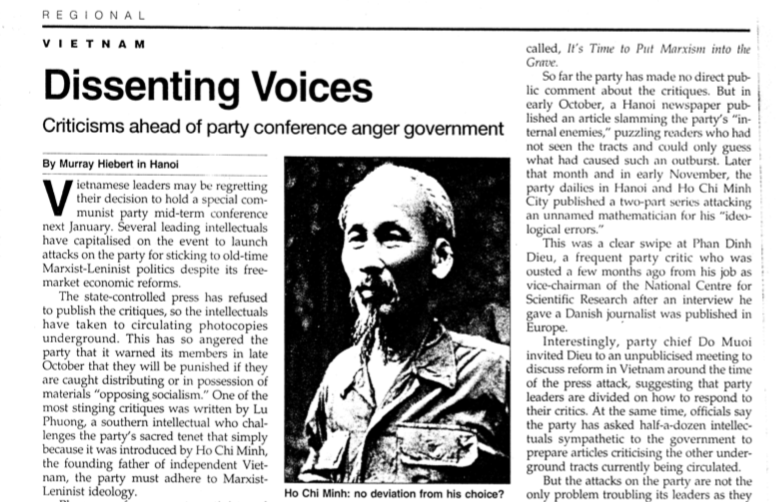
\includegraphics[scale=.4]{FE3}
\end{figure}

  
%\clearpage{\pagestyle{empty}\cleardoublepage}
  %\includepdf[pages=1-,noautoscale,pagecommand={\thispagestyle{plain}}]{Docs/1993_12_FarEasrtenEconomicReview.pdf}
\noindent REGIONAL VIETNAM\\
\begin{center}
 \textbf{Dissenting Voices}
\end{center}

\begin{center}
Criticisms ahead of party conference anger government
\end{center}

\textbf{By Murray Hiebert in Hanoi}

Vietnamese leaders may be regretting their decision to hold a special communist party mid-term conference next January. Several leading intellectuals have capitalised on the event to launch attacks on the party for sticking to old-time Marxist-Leninist politics despite its free-market economic reforms.


The state-controlled press has refused to publish the critiques, so the intellectuals have taken to circulating photocopies underground. This has so angered the party that it warned its members in late October that they will be punished if they are caught distributing or in possession of materials "opposing socialism." One of the most stinging critiques was written by Lu Phuong, a southern intellectual who challenges the party sacred tenet that simply because it was introduced by Ho Chi Minh, the founding father of independent Vietnam, the party must adhere to Marxist - Leninist ideology. 
	
	
Phuong, a former party activist and Culture Ministry official, argues that Ho simply "borrowed Leninism as a tool" to fight the French colonialists and the US. He never imagined that he had adopted an ideology which would "turn intelligent people into foolish ones, turn people with ideals into degenerate ones and bog down the nation in stagnation," Phuong writes.


"The incompetence in economic development and brutal suppression of politics and culture brought by the socialist model on behalf of Marx and proletarian revolution resulted in Vietnam for many years having independence, but not liberty and happiness," Phuong, who now works as a photographer in Ho Chi Minh City, writes in his 16-page tract.


"… economic development can only accompany political liberalisation ," he warns the party. "We have to give up the idealism that Uncle Ho chose in a very simple manner . . . But the question is by what means - will it come through collapse or will it come through peaceful means?"


Another critique circulating in the capital was authored by biology Prof. Nguyen Xuan Tu, writing under the pseudonym "Ha Si Phu," or "hero professor of Hanoi." Marxism-Leninism has been "unable to achieve national reconciliation [and] the construction of a democratic society and a market economy’’. Tu argues in his 76-page Paper.


"It is necessary for us to give up a foreign theory which is not suitable for our country . . . so that we can abolish [internal] resentment, call for contributions to develop the country and create conditions to harmonise our nation into the larger world," he writes.


"Some people are afraid that 'if we give up idealism we will suffer immediate chaos,"' Tu says, alluding to the party's argument that political reform will cause instability, threatening the country's modest economic achievements since the communists launched their drive towards a free market in 7986. "If this is true, our nation is only worthy of being a slave [and] we cannot be independent."


A third underground tract written by u southern intellectual, Nguyen Phong Ho Hieu, explores the ramifications of a possible US lifting of its trade embargo against Vietnam. Hieu, who quit the party in 1990, claims Hanoi's leaders are ambivalent about a US return to Vietnam because of the political impact of the anticipated surge in economic growth.


"The question of political liberty will arise when the people have economic freedom," Hieu argues. "People will demand that the government and party give back he liberties they have lost," he says, listing examples such as free elections, freedom of speech, press and religion, and equality before the law.


Overseas Vietnamese have also smuggled into the country documents criticising the party. One circulating in Hanoi is called, \textit{It’s Time to Put Marxism into the Grave}.


So far the party has made no direct public comment about the critiques. But in early October, a Hanoi newspaper published an article slamming the party's "internal enemies," puzzling readers who had not seen the tracts and could only guess what had caused such alt outburst. Later that month and in early November, the party dailies in Hanoi and Ho Chi Minh City published a two-part series attacking an unnamed mathematician for his "ideological errors."


This was a clear swipe at Phan Dinh Dieu, a frequent party critic who was ousted a few months ago from his job as vice-chairman of the National Centre for Scientific Research after an interview he gave a Danish journalist was published in Europe.


Interestingly, party chief Do Muoi invited Dieu to an unpublicised meeting to discuss reform in Vietnam around the time of the press attack, suggesting that party leaders are divided on how to respond to their critics. At the same time, officials say the party has asked half-a-dozen intellectuals sympathetic to the government to prepare articles criticising the other under- ground tracts currently being circulated.


But the attacks on the party, are not the only problem troubling its leaders as they prepare for the conference. Originally scheduled for November, the meeting has already been postponed twice, first to December then to January, reportedly because of differences within the leadership. Rumours are now circulating in Hanoi that the meeting may be postponed again.


Although the party is united on the need for continuing reform, officials say the country's leaders are divided on the pace at which change should be introduced. 


Party sources say senior leaders are also divided over the appointment of roughly 15 new central committee members, who are to replace members expected to retire or lose their positions during the conference. These differences are due to be debated when the central committee begins its sixth plenum around 23 November.


The plenum will also seek to revise the draft political report prepared for the conference. The current draft, which reviews economic and political developments in the country since its seventh congress in 1991, prompted widespread criticism from provincial officials and government ministries when it was circulated a month ago. Some critics charged that the document was overly optimistic about the country's economic development since the launching of the reforms. Others complained that the draft failed to spell out the party's vision for Vietnam's future, including a definition of what exactly it means to have "a free market economy with a socialist-orientation under the leadership oi the state." $\blacksquare$

\newpage

\textbf{Khu vực Việt Nam}

\begin{center}
\textbf{Những tiếng nói bất đồng}
\end{center}

\begin{center}
Những phản biện trước Hội nghị của Đảng khiến Chính phủ khó chịu 
\end{center}

\textbf{Murray Hiebert ở Hà Nội thực hiện}


Các nhà lãnh đạo của Việt Nam có thể hối hận về quyết định tổ chức một Hội nghị đặc biệt của Đảng giữa kỳ vào tháng 1 tới. Một số trí thức hàng đầu đã tập hợp bàn luận trước sự kiện này để khởi động cuộc phản đối Đảng về việc tự gắn mình vào học thuyết Mác-Lê vốn đã lỗi thời. Mặc dù Đảng cũng đã có những cải cách kinh tế theo hướng thị trường tự do.  


Báo chí nhà nước từ chối đăng các bài báo mang tính phản biện vì thế, các trí thức đã truyền tay nhau những tài liệu được sao chép. Điều này cũng khiến cho Đảng khó chịu và Đảng cũng cảnh báo các Đảng viên hồi cuối tháng 10 là những ai bị bắt quả tang phân phát hoặc giữ những tài liệu “chống chủ nghĩa cộng sản” sẽ bị xử phạt. Một trong những phê bình gay gắt nhất là của ông Lư Phương – một trí thức miền Nam đã phê phán nguyên tắc thiêng liêng của Đảng cộng sản vì nó được ông Hồ Chí Minh khởi xướng - người cha già của Việt Nam độc lập – cho rằng Đảng phải đi theo đường lối tư tưởng hệ của Mác-Lê. 


Ông Phương - một người đã từng trong Đảng và từng là quan chức Bộ Văn Hóa lập luận ông Hồ chẳng qua là chỉ “mượn chủ nghĩa Lê nin như một thứ công cụ” để đấu tranh với thực dân Pháp và đế quốc Mỹ. Ông viết: “Chưa bao giờ ông Hồ nghĩ rằng ông ấy sẽ chấp nhận hệ tư tưởng đó mà nó sẽ “đẩy những người dân giỏi giang trở thành những kẻ ngu ngốc, biến con người ta với mớ lý luận trở thành những kẻ thoái hóa và kìm hãm đất nước trong sự trì trệ”.


Ông Phương hiện đang làm thợ chụp ảnh ở Thành phố Hồ Chí Minh viết một tiểu luận gồm 16 trang, trong đó có đoạn: “Sự thiếu năng lực trong phát triển kinh tế và đàn áp tàn bạo về chính trị và văn hóa của mô  hình chủ nghĩa cộng sản nhân danh chủ nghĩa Mác và cuộc cách mạng vô sản đã khiến cho Việt Nam mất nhiều năm mới có được sự độc lập nhưng không phải là sự giải phóng và hạnh phúc”.
 
 
 
“....phát triển kinh tế chỉ có thể song hành cùng tự do hóa chính trị”. Ông cảnh báo Đảng. “Chúng ta phải từ bỏ cái thứ chủ nghĩa mà ông Hồ lựa chọn theo một cách rất đơn sơ.... Nhưng vấn đề đặt ra là làm cách nào – có phải thông qua một sự sụp đổ hay điều đó sẽ được diễn ra trong cách thức ôn hòa?”.


Một bài phê bình khác cũng được lưu hành tại thủ đô Hà Nội do Giáo sư Sinh học - ông Nguyễn Xuân Tụ với bút danh “Hà Sĩ Phu” hoặc “Giáo sư anh hùng của Hà Nội” trong một tiểu luận dày 76 trang viết: “Chủ nghĩa Mác-Lê đã không thể giúp đạt được sự hòa giải dân tộc, đạt được việc xây dựng một xã hội dân chủ và đạt được một nền kinh tế thị trường”.


Ông viết: “Chúng ta cần phải loại bỏ ngay học thuyết của nước ngoài này vì nó không phù hợp với đất nước chúng ta....chỉ có thế mới bớt đi được những oán thán, mới kêu gọi đóng góp chung tay phát triển đất nước và tạo điều kiện cho việc cùng nhau đưa quốc gia hội nhập với thế giới đại đồng”. 


Ông nói: "Nhiều người e sợ rằng ‘nếu chúng ta từ bỏ chủ nghĩa này chúng ta phải gánh chịu hậu quả là sự hỗn loạn sẽ xảy ra” - điều đó hàm ý luận điểm của Đảng cho rằng cải cách chính trị sẽ gây nên bất ổn, đe dọa những thành tựu phát triển kinh tế hiện nay của đất nước kể khi Đảng cộng sản tiến hành công cuộc đổi mới từ năm 1986. “Nếu điều đó đúng, quốc gia chúng ta chỉ xứng đáng làm nô lệ chứ chúng ta không có độc lập”.


Một bài viết thứ ba khác cũng ngầm được lưu hành là của một trí thức miền Nam – ông Nguyễn Phong Hồ Hiếu – đã phát hiện ra những chia rẽ qua việc Mỹ rút lệnh cấm vận thương mại với Việt Nam. Ông Hiếu là người ra khỏi Đảng năm 1990, ông từng tuyên bố các Lãnh đạo ở Trung ương rất mơ hồ trước việc Hoa Kỳ quay trở lại Việt Nam vì những tác động chính trị đối với tăng trưởng kinh tế được dự báo trước. 


Ông Hiếu lập luận: "Vấn đề tự do chính trị sẽ nảy sinh khi người dân có tự do kinh tế". "Mọi người sẽ yêu cầu chính phủ và Đảng phải trao lại quyền tự do mà họ đã bị mất”. Ông cũng kể ra một số ví dụ như bầu cử tự do, tự do ngôn luận, tự do báo chí và tự do tôn giáo cũng như bình quyền trước luật pháp. 

Người Việt Nam ở hải ngoại cũng lén lút đưa vào trong nước những tài liệu phê phán Đảng. Một văn bản được lưu hành tại Hà Nội có tiêu đề \textit{Đến lúc khai tử Chủ nghĩa Mác}. 


Đến bây giờ Đảng cũng chưa có lời bình luận công khai về những phản biện nhưng đầu tháng 10, một tờ báo ở Hà nội  công bố một bài đánh thẳng vào những “kẻ thù nội bộ” của Đảng gây khó hiểu cho độc giả - những người không thấy được sự thật mà chỉ dò đoán điều gì đã khiến bùng phát chuyện tày đình. Cuối tháng 10 đầu tháng 11, tờ Nhân Dân của Đảng tại Hà Nội và Thành Phố Hồ Chí Minh đã công bố loạt bài gồm hai phần tấn công nhà toán học không tiết lộ tên về “những sai lầm trong tư tưởng” của vị này.


Rõ ràng đây là cú hất cẳng giáo sư Phan Đình Diệu – một nhà phản biện thường xuyên đối với Đảng, người đã bị tước chức vụ cách đó vài tháng khi ông còn là phó chủ tịch Trung Tâm Nghiên Cứu Khoa Học Quốc Gia sau khi ông trả lời phỏng vấn phóng viên Đan Mạch và bài báo được công bố tại Châu Âu.


Điều thú vị là chính Tổng bí thư Đỗ Mười đã mời giáo sư Diệu đến một cuộc họp kín để trao đổi về cải cách ở Việt Nam trong khoảng thời gian xảy ra cuộc tấn công báo chí. Điều đó cho thấy các Lãnh đạo Đảng phân công nhau để đối phó với những chỉ trích về mình. Đồng thời, các quan chức cũng cho biết Đảng đã tham khảo hơn nửa số trí thức cùng chung sự cảm thông với chính phủ để chuẩn bị cho các bài viết phê phán các lực lượng chống phá ngầm đang tồn tại.


Các cuộc công kích Đảng thì không phải là mối quan tâm duy nhất khiến các nhà Lãnh đạo phải quan ngại vì họ đang phải chuẩn bị cho Hội nghị sắp diễn ra. Dự kiến lúc đầu hội nghị sẽ diễn ra vào tháng 11 nhưng đã phải hoãn đến hai lần, lần 1 vào tháng 12 và sau đó tận tháng 1. Theo tin cho hay việc trì hoãn này cũng là do những bất đồng trong chính đội ngũ lãnh đạo. Nhiều đồn đoán trong xã hội Hà Nội lúc bấy giờ là có khi Hội nghị sẽ tiếp tục bị trì hoãn.


Mặc dù Đảng thống nhất về sự cần thiết phải tiếp tục cải cách, các quan chức cho biết do các lãnh đạo được bổ nhiệm theo đó sẽ có những bước thay đổi theo nhiệm kỳ. 


Các nguồn tin của Đảng cho biết các lãnh đạo cấp cao cũng đang phân chia việc bổ nhiệm khoảng 15 tân ủy viên trung ương – những người sẽ thay thế một số thành viên sẽ nghỉ hưu hoặc mất ghế trong khi hội nghị diễn ra. Những khác biệt trên sẽ được đưa ra tranh luận khi Hội nghị trung ương bắt đầu kỳ họp thứ 6 vào khoảng thời gian 23 tháng 11. 


Tại hội nghị này, Đảng sẽ xem xét dự thảo báo cáo chính trị chuẩn bị trình Đại hội. Dự thảo xem xét đánh giá tình hình phát triển kinh tế, chính trị tại Việt Nam kể từ Đại hội VII năm 1991 đã dấy lên những phản biện, phê bình từ các bộ, ngành và quan chức các tỉnh, thành phố khi Dự thảo này được lưu truyền cách đây khoảng một tháng. Nhiều bài phê bình cáo buộc văn bản này đã quá lạc quan về hiện tình kinh tế của đất nước kể từ khi thực hiện đổi mới. Nhiều ý kiến khác phê bình Dự thảo lần này không nêu ra tầm nhìn của Đảng đối với tương lai quốc gia, gồm cả việc đưa ra định nghĩa thế nào là “một nền kinh tế thị trường theo định hướng xã hội chủ nghĩa dưới sự lãnh đạo của nhà nước”.



\chapter{Un Jeune Scientifique}\index{Báo chí}
\begin{figure}
\centering
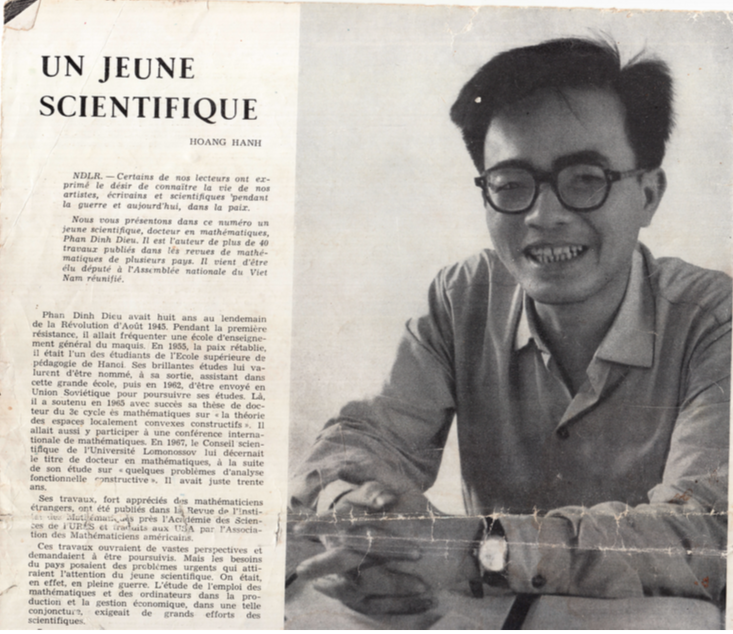
\includegraphics[scale=.3]{Un}
\end{figure}
  
%\clearpage{\pagestyle{empty}\cleardoublepage}
%  \includepdf[pages=1-,scale=0.85,pagecommand={\thispagestyle{plain}}]{Docs/197%x_UnJeuneScientifique.pdf}
 HOANG HANH 
 

\begin{quote}
 \textit{NDLR. - Certains de nos lecteurs ont exprimé le désir de connaitre la vie de nos artistes, écrivains et scientifiques pendant la guerre et aujourd'hui, dans la paix. }

 \textit{Nous vous présentons dans ce numéro un jeune scientifique, docteur en mathématiques, Phan Dinh Dieu. Il est l'auteur de plus de 40 travaux publiés dans les revues de mathématiques de plusieurs pays. Il vient d'être élu député à l'Assemblée nationale du Viet Nam réunifié.}
\end{quote}

​
Phan Dinh Dieu avait huit ans au lendemain de la Révolution d'Août 1945. Pendant la première résistance, il allait fréquenter une école d'enseignement général du maquis. En 1955, la paix rétablie il était l'un des étudiants de l'Ecole supérieure de pédagogie de Hanoi. Ses brillantes études lui valurent d'être nommé, à sa sortie, assistant dans cette grande école, puis en 1962, d'être envoyé en Union Soviétique pour poursuivre ses études. Là, il a soutenu en 1965 avec succès sa thèse de docteur du 3e cycle ès mathématiques sur ‘la théorie des espaces localement convexes constructifs’. Il allait aussi y participer à une conférence internationale de mathématiques. En 1967, le Conseil scientifique de l'Université Lomonossov lui décernait le titre de docteur en mathématiques, à la suite de son étude sur ‘quelques problèmes d'analyse fonctionnelle constructive’. Il avait juste trente ans.


Ses travaux, fort appréciés des mathématiciens étrangers, ont été publiés dans la Revue de l'Institut ces Les Mathématiques des près l'Académie des Sciences de l'URUS et traduits aux USA par l'Association des Mathématiciens américains.

Ces travaux ouvraient de vastes perspectives et demandaient à être poursuivis. Mais les besoins du pays posaient des problèmes urgents qui attiraient l'attention du jeune scientifique. On était en effet, en pleine guerre. L'étude de l'emploi des mathématiques et des ordinateurs dans la pro et la gestion économique, dans une telle conjoncture, exigeait de grands efforts des scientifiques. 

Comme tant autre, il vivait et travaillait, loin de sa femme et de ses enfants évacués, dans des conditions de guerre des plus pénibles. Livres et autres documents de travail mettaient beaucoup de temps à lui parvenir. Pourtant, il a mis au point plusieurs ouvrages de mathématiques de va valeur, participé à la formation de jeunes cadres de l'Institut de Mathématiques du Viet Nam et enseigné les mathématiques, à l’Ecole supérieure de pédagogie de Hanoi, à l’Ecole polytechnique à l'Institut Hanoi des Mathématiques. 
​
Je suis allé le voir chez lui un dimanche matin. Je l'ai trouvé en train d'enseigner l'écriture à sa jeune fille de huit ans, Quynh. ‘‘Quelle mauvaise écriture pour une élève de deuxième’’ (1), me dit-il avec le sourire, après avoir arrêté la leçon.

Il m'a raconté être né dans une province pauvre, le Nghe Tinh, d'une mère paysanne, et avoir manié la charrue dans ses jeunes années. 
 	-J'ai à peine commencé mes recherches, a-t-il poursuivi, et il est encore trop tôt pour émettre un jugement de valeur sur mes travaux. 
-Que signifie pour vous d'avoir été élu député par les paysans de la province de Thai Binh lui ai-je demandé. 
-J'en suis très fier, a-t-il répondu, les yeux brillant de satisfaction. Je m'efforcerai de mériter la confiance de ces paysans dont je suis moi-même issu.
 (1) L'équivalent de la 9e dán le système francais. 



\part{Khoa Học và Giáo Dục }
\clearpage{\pagestyle{empty}\cleardoublepage}
\section{BOOK on AMS}
\url{http://books.google.fr/books?id=dfAB9E0WqyUC&lpg=PP1\break &hl=fr&pg=PP1#v=onepage&q&f=false}
\begin{center}
    \begin{figure}[htp]
    \begin{center}
     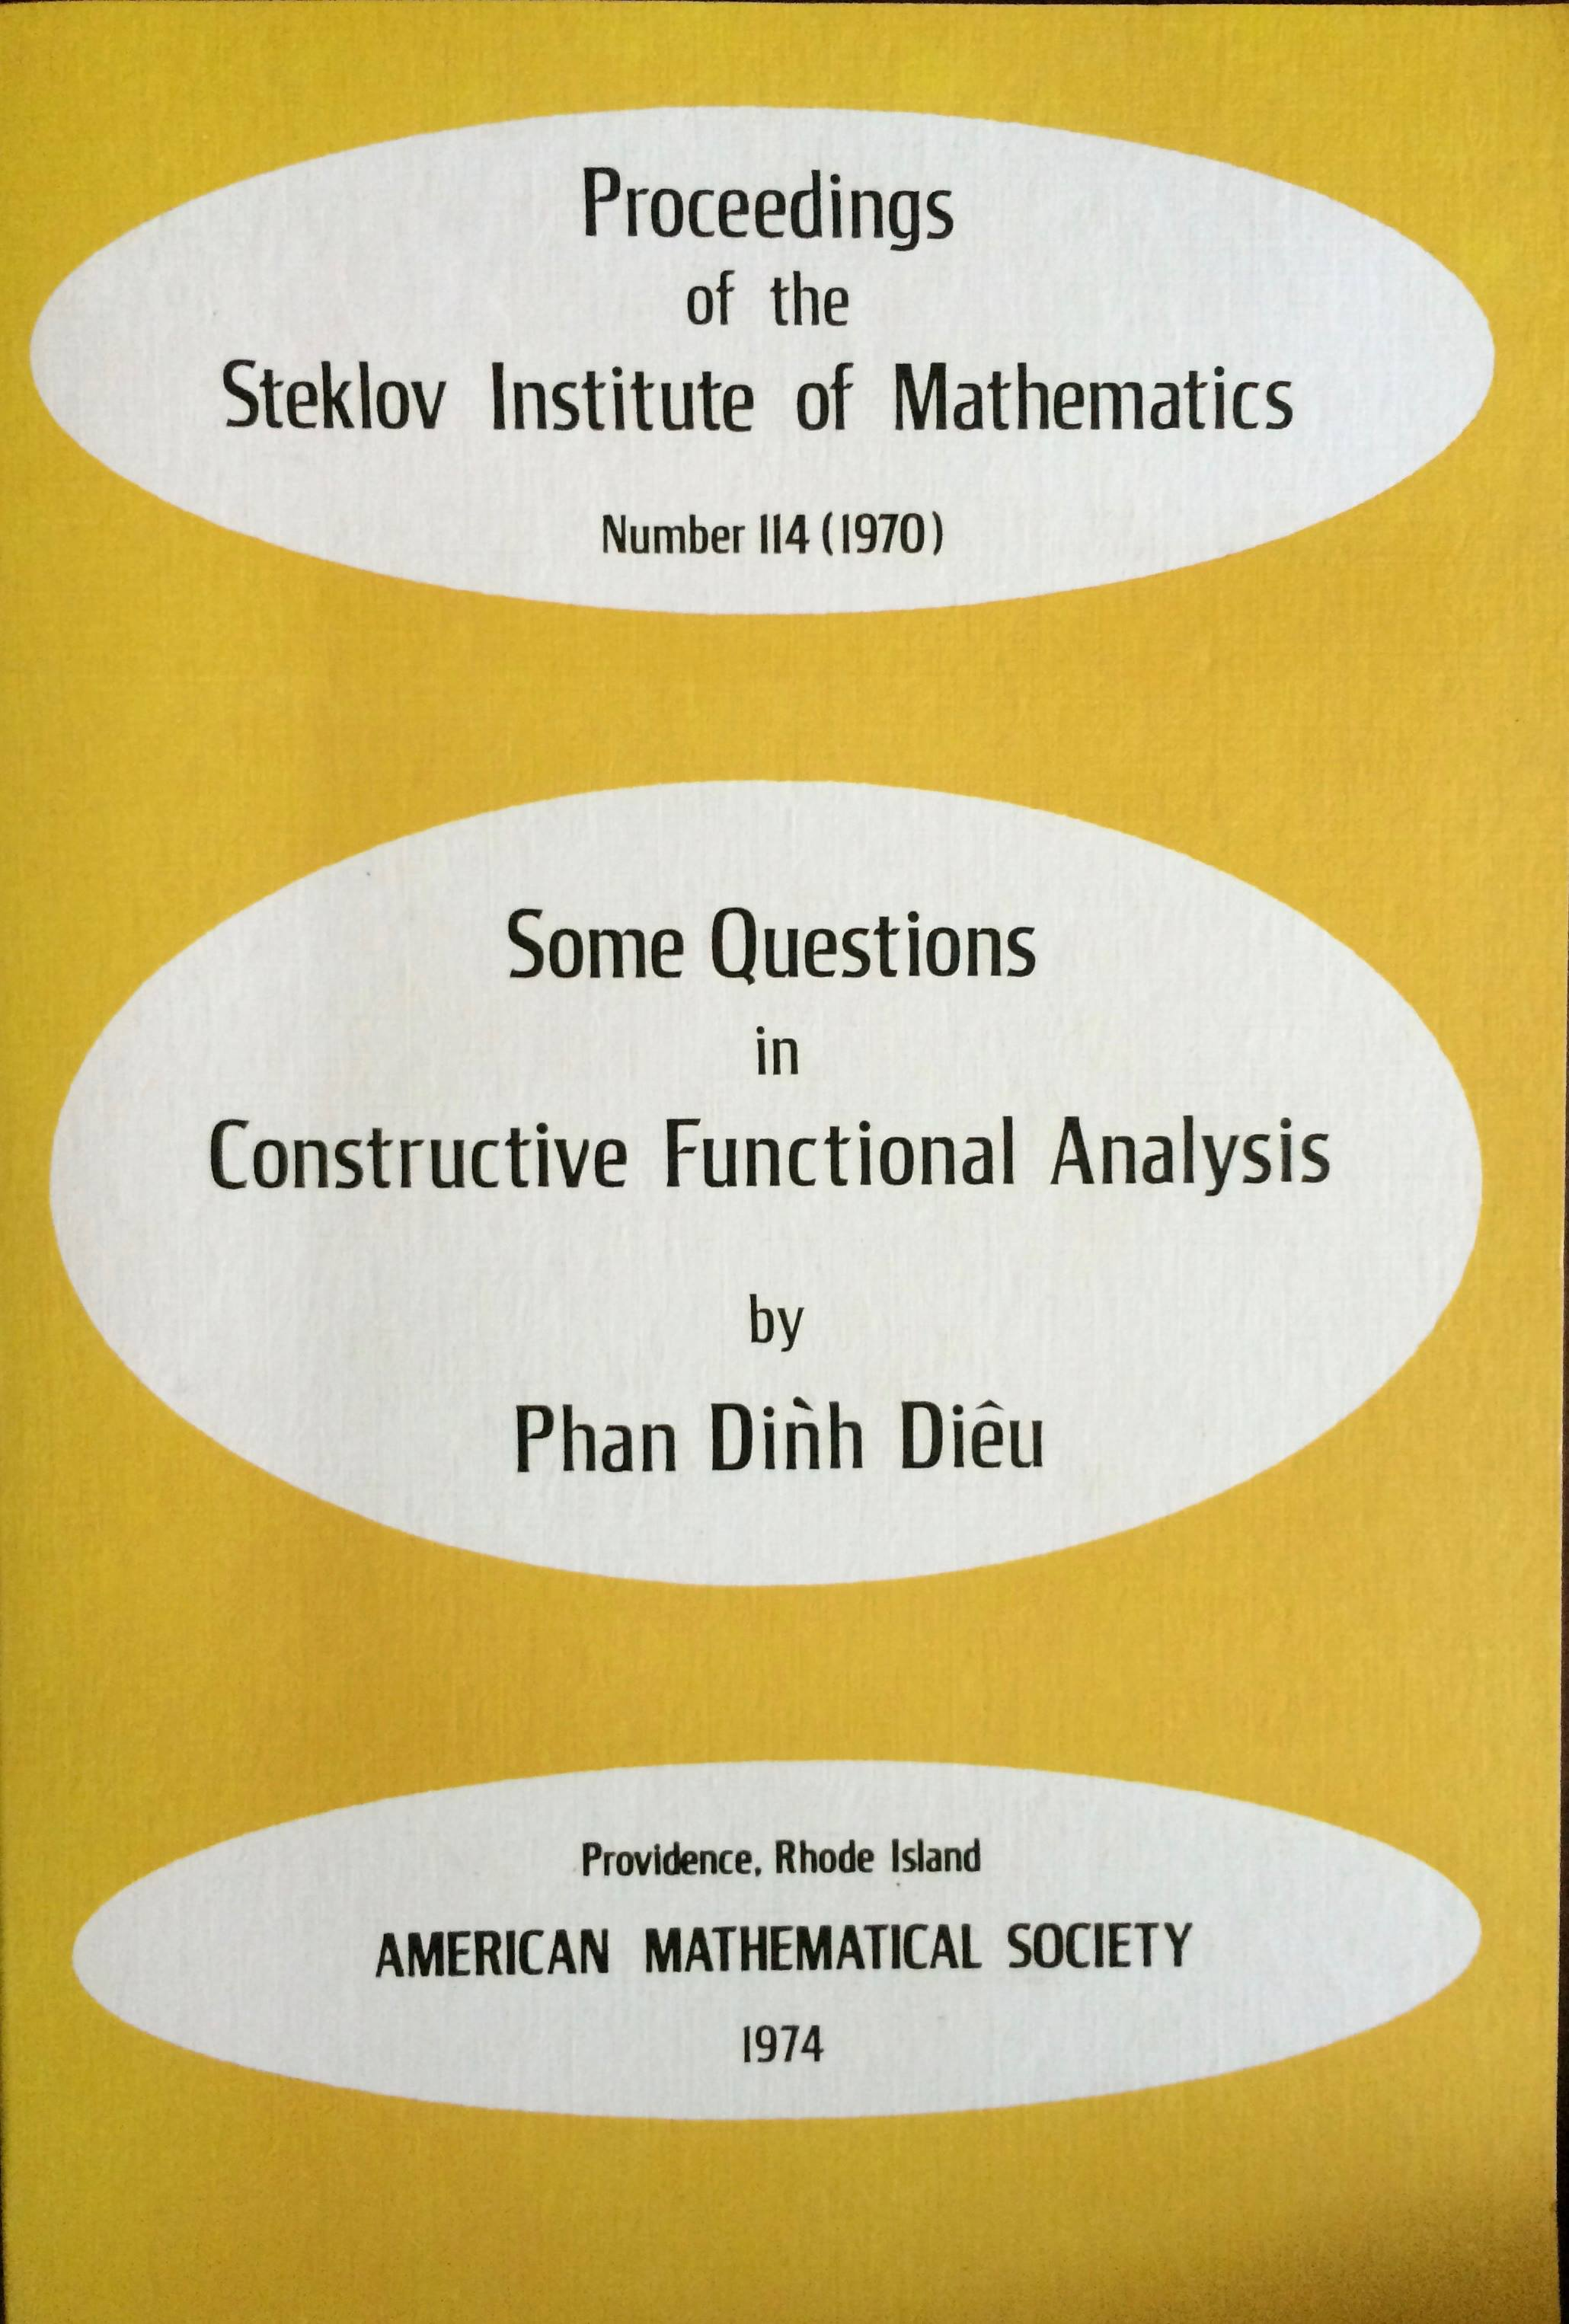
\includegraphics[scale=.1]{BiaSach.jpg}
    \end{center}
    %\caption{Cái sẽ hiển thị bên dưới hình}
   % \label{refhinh1}
    \end{figure}
\end{center}
\newpage
\section{Về một chính sách Tin học}

\begin{center}
    \begin{figure}[htp]
    \begin{center}
     \includegraphics[scale=.5]{30_NamVienCNTT}
    \end{center}
    \end{figure}
\end{center}

Bản báo cáo này gồm các phần sau đây:

\begin{itemize}
\item[ ]Phần I. Ngành tin học trong cuộc CMKHKT hiện nay và yêu cầu cấp thiết của một chính sách.
\begin{itemize}
\item[I.] Tin học trong CMKHKT hiện nay
\item[II.] Tin học đối với chúng ta và yêu cầu của một chính sách.
\end{itemize}
\item[ ]Phần II. Mục tiêu và nội dung của việc xây dựng và phát triển ngành tin học.
\begin{itemize}
\item[I.] Mục tiêu
\item[II.] Ứng dụng tin học, hay từng bước tin học hóa nền kinh tế xã hội của ta
\item[III.] Xây dựng công nghiệp tin học
\end{itemize}
\item[ ]Phần III. Các chính sách và biện pháp chủ yếu
\begin{itemize}
\item[I.] Con người. Đào tạo và nghiên cứu tin học
\item[II.] Vốn đầu tư và trang bị kỹ thuật
\item[III.] Quan hệ quốc tế và vấn đề tiếp thu tiến bộ KHKT
\item[IV.] Về tổ chức và quản lý.
\end{itemize}
\end{itemize}

Bản báo cáo này được viết trên cơ sở tiếp thu các ý kiến thảo luận trong Hội đồng khoa học ngành Tin học của UBKHKTNN, cũng như các bản sơ thảo về chính sách phát triển tin học do Viện KHVN và UBKHKTNN chuẩn bị trước đây, do Tổng cục Điện tử và ký thuật tin học đề xuất gần đây.

\begin{center}
\textbf{\underline{ PHẦN THỨ NHẤT}}
\end{center}

Ngành Tin học trong cuộc cách mạng Khoa học Kỹ thuật hiện nay và yêu cầu cấp thiết của một chính sách Tin học

\textbf{I.	\underline {Tin học trong cách mạng KHKT hiện nay.}}


1.	Đối tượng của Tin học là thông tin và các quá trình xử lý thông tin tự động bằng máy tính điện tử. Những tiến bộ cực kỳ nhanh chóng và sự thâm nhập sâu rộng của Tin học trong mọi lĩnh vực của sản xuất và kinh tế - xã hội là một đặc điểm nổi bật của cuộc cách mạng KHKT hiện nay, là một tiến bộ KHKT mũi nhọn của thời đại, Tin học cung cấp các phương pháp và công cụ cực kỳ mạnh mẽ giúp con người khai thác và xử lý thông tin, do để được ứng dụng có hiệu quả trong các lĩnh vực nghiên cứu khoa học kỹ thuật, điều khiển tự động các quá trình công nghệ, trong điều tra cơ bản, trong thông tin liên lạc, v.v. Và đặc biệt quan trọng là việc ứng dụng tin học trong lĩnh vực tổ chức và quản lý: quản lý sản xuất, quản lý kinh tế và xã hội,… Vì thông tin tồn tại và vận động trong hầu hết mọi lĩnh vực hoạt động của con người và xã hội, nên tin học đang có xu hướng thâm nhập sâu rộng vào tất cả các lĩnh vực hoạt động để tạo nên những biến đổi sâu sắc về chất lượng và hiệu quả của các hoạt động đó. Mặt khác, việc sản xuất các máy tính điện tử và các sản phẩm tin học đã hình thành nên một ngành công nghiệp tin học trên thế giới; trong một số nước rất phát triển, ngành công nghiệp này đang vươn lên vị trí của một trong những ngành công nghiệp hàng đầu. Lao động trong khu vực thông tin không ngừng tăng lên, và tỷ trọng thu nhập xã hội do khu vực này mang lại cũng ngày càng lớn, cùng với việc điện tử hóa, công việc “tin học hóa” đang mang lại những biến đổi sâu sắc trong cơ cấu sản phầm và cơ cấu giá trị của nền kinh tế xã hội, và vì vậy là một yếu tố cách mạng đối với nền sản xuất về kinh tế trong giai đoạn hiện nay của cuộc cách mạng khoa học – kỹ thuật.


2.	 Về mặt khoa học kỹ thuật, trong giai đoạn hiện nay và 10-15 năm tới, tin học được phát triển theo các phương hướng chủ yếu sau đây:


2.1.	 Máy tính điện tử không ngừng được nâng cao về hiệu quả và chất lượng. Về chất lượng xử lý, từ chỗ là công cụ tính toán và xử lý thông tin, máy tính điện tử sẽ tiến lên , nó có khả năng tích lũy trí thức, xử lý trí thức và thực hiện chức năng “trí tuệ nhân tạo’. Về năng lực xử lý, hiện đã có các máy tính điện tử với tốc độ hàng trăm triệu phép tính một giây, trong một số năm tới sẽ có những máy tính điện tử với tốc độ xử lý hàng tỷ, hàng chục tỷ phép tính một giây, những máy tính này sẽ có kiến trúc phi cổ điển, có khả năng xử lý song song (trong một máy có thể có hàng vạn đến hàng triệu bộ xử lý làm việc đồng thời). Khả năng máy tiếp nhận thông tin trực tiếp từ ngôn ngữ tự nhiên, bằng tiếng nói, hình sẽ dần dần trở thành hiện thực. Mặc dù trong một số năm tới, các “siêu máy tinh” với những khả năng như vậy chưa phải được sử dụng phổ biến, nhưng những quan điểm hiện đại về chất lượng và kiến trúc mới của máy tính là rất đáng được quan tâm.


2.2.	Sự ra đời và tiến bộ nhanh chóng của kỹ thuật vi xử lý mở ra một giai đoạn mới có tính chất cách mạng trong tin học. Sau một thời ký thử thách, ngày nay các máy vi tính trên cơ sở kỹ thuật vi xử lý đã chiếm lĩnh một vị trí chắc chắn và ngày càng vững vàng trong việc ứng dụng tin học vào mọi lĩnh vực hoạt động của xã hội. Với tiến bộ nhanh chóng của kỹ thuật vi điện tử, các máy vi tính ngày càng có khả năng lớn, vượt khỏi phạm vi của “máy tính cá nhân” và trở thành máy tính chuyên nghiệp. Các máy vi tính với giá mua vài ba ngàn đô la, với khả năng tính toán khá mạnh (tốc độ có thể đến triệu phép tính/giây, bộ nhớ trong 1-2 megabytes, phần mềm phong phú,…) là công cụ hấp dẫn đối với mọi cơ sở sản xuất, kinh doanh, dịch vụ, v.v… Hằng năm, trên thị trường thế giới có thêm khoảng 5 triệu máy vi tính. Ngoài máy vi tính, cũng cần chú ý là kỹ thuật vi xử lý có thể được ứng dụng một cách mềm dẻo, đa dạng trong nhiều lĩnh vực kỹ thuật và sản xuất. Kỹ thuật vi xử lý và máy vi tính, với khả năng thâm nhập sâu rộng của mình, là công cụ vô cùng đắc lực cho việc tin học hóa xã hội hiện nay và tương lai.


2.3.	Kết hợp với những tiến bộ to lớn cả kỹ thuật thông tin liên lạc, người ta đã xây dựng các mạng máy vi tính điện tử với khả năng thực hiện các hệ thống lưu trữ, truyền đưa và xử lý thông tin ở mọi quy mô khác nhau, từ mức xí nghiệp, ngành cho đến quy mô quốc gia và quốc tế - Điều đó làm cho khả năng và hiệu quả của việc khai thác và sử dụng các nguồn thông tin trong mọi hoạt động của xã hội tăng kên nhanh chóng làm tiền đề cho những đổi thay to lớn trong việc tổ chức các hoạt động kinh tế và xã hội.


3.	Ta chú ý một số đặc điểm sau đây trong sự phát triển hiện nay của Tin học:


3.1	Trong khi việc ứng dụng Tin học có phạm vi ngày càng rộng rãi đối với mọi quốc gia, thì ngành công nghiệp sản xuất các linh kiện và thiết bị tin học lại là một ngành mũi nhọn, đòi hỏi đầu tư lớn và một cơ sở công nghiệp hiện đại, nên thực tế đang tập trung trong tay một số ít nước phát triển nhất. Thí dụ đối với các linh kiện cao cấp như các mạch vi xử lý, các mạch nhớ dung lượng lớn, thì gần như toàn bộ được sản xuất ở Mỹ, một phần ở Nhật (không kể ở các nước XHCN). Ngay cả những nước như CHLB Đức cũng phải nhập khoảng 80\% linh kiện cho công nghiệp Tin học của mình. Trong số 50 hãng sản xuất máy tính lớn nhát của thế giới tư bản, thì hơn 40 hãng lẻ của Mỹ, riêng hãng có chỉ số kinh doanh về KTĐT bùng một nửa chỉ số kinh doanh về KTĐT của thế giới.


3.2	Trong khi tiến bộ kỹ thuật làm cho phần cứng đạt được tốc độ tăng năng suất cao, thì tốc độ tăng năng suất phần mềm đạt được còn khá thấp. Trong việc ứng dụng tin học, chi phí cho phần mềm chiều một tỷ lệ ngày càng cao so với phần cứng (đối với các nước phát triển hiện nay là khoảng 85\% - 15\%). Cơ cấu phần mềm lại rất đa dạng, có những phần mềm cơ bản mà chỉ các hãng sản xuất máy tính hoặc một số ít cơ sở nghiên cứu liên quan làm ra, nhưng có một phạm vi mênh mông của phần mềm ứng dụng mà bất kỳ ai nghiên cứu và ứng dụng tin học có khả năng cũng đều cần và có thể làm được. Vì sản phẩm phần mềm chiếm một tỷ lệ giá trị lớn, và vốn đầu tư để tạo cơ sở vật chất – kỹ thuật cho nó không đòi hỏi nhiều như sản xuất phần cứng, nên nhiều nước xem đây là một chỗ có thể cứ để xác định phương hướng phát triển tin học của mình. 


3.3. Tin học được xem là ngành sản mũi nhọn chiếm vị trí hàng đầu trong chính sách Khoa học – Kỹ thuật và phát triển Kinh tế của các nước tư bản phát triển. Các nước xã hội chủ nghĩa trong khối SEV cũng đã xác định Tin học là một trong năm hướng ưu tiên phát triển và hợp tác. Nhiều nước trong thế giới thứ ba cũng đã xác định chính sách tin học của mình.


 Trong vùng Đông Á, ngoài Nhật Bản, sự phát triển nhanh chóng và hiệu quả của một số nước “công nghiệp mới” đang được lưu ý. Nam Triều Tiên và Đài Loan đang vươn lên thành những nước sản xuất và xuất khẩu của linh kiện điện tử cao cấp (như các mạch nhớ) và máy vi tính cùng thiết bị ngoại vi. Công nghiệp phần mềm được xem là chiến lược phát triển của Singapore, v.v….
 
 
\textbf{II. \underline{Tin học đối với chúng ta và yêu cầu của một chính sách.}}


1.	Ở nước ta, việc sử dụng máy tính điện tử được bắt đầu từ cuối những năm 60. Việc sử dụng KTĐT trong gia đoạn trước 1975 đã thúc đẩy bước đầu việc xây dựng ngành Tin học và việc nghiên cứu, ứng dụng Tin học trong nhiều ngành xây dựng, giao thông vận tải, lâm nghiệp, khí tượng thủy văn, thủy lợi, v.v… Trước năm 1975, ở miền Nam, ngoài mục đích quân sự, máy tính điện tử cũng đã được ứng dụng có nền nếp và hiệu quả trong các hoạt động thống kê, hạch toán và quản lý xí nghiệp. Sau khi giải phóng miền Nam, ta tiếp thu được hơn 20 máy tính điện tử loại IBM 360 (từ model 20 đến 50), và nhiều máy vẫn tiếp tục làm việc đến nay tuy có nhiều khó khăn.


Trong các năm 1975 và 1976, Hội đồng Chính phủ đã hai lần ra các nghị quyết 173(1975) và 245 CP (1976) về việc tăng cường quản lý và sử dụng MTĐT trong quản lý kinh tế và tăng cường quản lý và sử dụng MTĐT trong cả nước, và do đó đã lập các viện nghiên cứu về kinh tế về khoa học tính toán và điều khiển. Từ năm 1975 đến đầu những năm 1980, tuy Nhà nước đã có các nghị quyết như vậy, nhưng do có nhiều biến động và khó khăn về tình hình chung, nên chưa có các biện pháp tích cực để thực hiện đầy đủ các nghị quyết đó. Các vấn đề ứng dụng Tin học có được tăng lên ít nhiều, nhưng chưa có những đóng góp đáng kể trong các lĩnh vực quan trọng của sản xuất và quản lý kinh tế. Do không có đầu tư thêm về trang bị MTĐT, nên ở khu vực phía bắc, việc nghiên cứu và ứng dụng có nhiều hạn chế. Ở khu vực phía Nam, bên cạnh một số cơ sở duy trì và phát triển được việc sử dụng các MTĐT vốn có, nhiều cơ sở khác do những thay đổi về cấu và tổ chức chưa sử dụng tốt các MTĐT. Bên cạnh đó, do tác động của những tiến bộ to lớn của kỹ thuật tin học trên thế giới, mốt số cơ sở nghiên cứu đã bước đầu đào tạo cán bộ, tiến hành nghiên cứu và ứng dụng các tiến bộ kỹ thuật mới, đặc biệt là kỹ thuật vi xử lý và vi tin học.


 Từ năm 1983 lại đây, sự thâm nhập của các máy vi tính theo nhiều đường khác nhau, cộng thêm việc nhập máy theo các chương trình viện trợ đã tạo ra những nét mới trong việc trang bị MTĐT trong cả nước. Chúng ta có thêm một số mát tính mini như NINI6, 1-6, và khoảng trên dưới 100 máy vi tính các kiểu Apple-II, IBM-FC, v.v… Điều này đã thúc đẩy việc ứng dụng Tin học trong sản xuất và kinh tế ở một giai đoạn mới, và rõ ràng đặt ra nhiều vấn đề cần được xem xét và giải quyết. Về mặt tổ chức, việc thành lập Tổng cục điện tử và kỹ thuật tin học vào năm 1984 là một bước tiến quan trọng trong việc xây dựng và phát triển ngành điện tử và tin học ở nước ta.
 
 
2.	Thực tiễn nghiên cứu và ứng dụng Tin học trong thời gian vừa qua, tuy chưa nhiều, cũng có thể cho chúng ta rút ra vài nhận định về những kết quả và khả năng, cũng như về những thiếu sót và khó khăn mà chúng ta cần tính đến trong sự phát triển Tin học sắp tới.


2.1.	 Một trong những yếu tố quan trọng là cán bộ KHKT của ta có khả năng tiếp thu những tiến bộ KHKT hiện đại đặc biệt trong lĩnh vực tin học. Trong mấy năm qua, tuy chưa nhiều, nhưng ta cũng đã tạo được một số tập thể cán bộ, kỹ sư tiếp thu, làm chủ và vận dụng được các trí thức hiện đại về kỹ thuật vi xử lý và vi tin học, về phần mềm .v.v. Trong công tác ứng dụng vào các ngành, đã có một số tập thể có kinh nghiệm trong một số lĩnh vực như thủy lợi, điện lực, lâm nghiệp, xây dựng, quản lý, v.v…


Nhu cầu tiềm năng của việc ứng dụng thì rất lớn. Nhưng hình thành được các nhu cầu có thể đáp ứng một cách hiện thực và có hiệu quả trong từng giai đoạn là điều rất quan trọng. Qua thực tiễn ứng dụng vừa qua, ta đã có khả năng hình thành được các nhu cầu hiện thực như vậy và trong chừng mực nhất định, có chuẩn bị những điều kiện để đáp ứng các nhu cầu đó.


2.2.	 Trong mấy năm qua, sự chậm trễ của ta trong việc đào tạo cán bộ tin học là một thiếu sót quan trọng, làm cho hiện nay, khi đứng trước nhu cầu phát triển và ứng dụng tin học một cách rộng rãi thì ta không có đủ cán bộ có hiểu biết để triển khai thực hiện. Ta đã có một số tổ chức về tin học nhưng các mặt công tác nghiên cứu, đào tạo, sản xuất, ứng dụng và dịch vụ chưa được phối hợp một cách có hiệu quả để phát huy đầy đủ lực lượng tin học chung của chúng ta. Tình trạng phân tán, thiếu sự hợp tác và trao đổi trí thức, kinh nghiệm với nhau là không có lợi cho sự phát triển nhanh việc ứng dụng Tin học của ta. Hiện nay, tuy số máy tính chưa nhiều, nhưng do thiếu cán bộ và do tình trạng phân tán cục bộ nói trên, nên các phương tiện hiện có chưa được sử dụng hợp lý, nhiều khi còn lãng phí.


3.	Xây dựng và phát triển tin học để đáp ứng các nhu cầu phát triển của sản xuất, kinh tế và các mặt hoạt động xã hội khác là một đòi hỏi khách quan, không thể lảng tránh được. Đã đến lúc chúng ta phải thật sự tích cực và chủ động nắm lấy việc xây dựng và phát triển ngành KHKT mũi nhọn này phù hợp với hoàn cảnh và khả năng của ta để đưa nó phục vụ đắc lực cho sự phát triển kinh tế xã hội của nước ta. Ta phải xác định rõ cái ta muốn đạt được. Không chỉ ta làm được và có thể nỗ lực để làm được, và cả những cách thức tận dụng sự nỗ lực để nhằm đạt được một cách tốt nhất mục tiêu của chúng ta.


Nói cách khác, ta phải xác định một chính sách xây dựng ngành Tin học, và xem việc thực hiện chính sách đó là một trong những nhiệm vụ Kinh tế và KHKT quan trọng trong giai đoạn sắp tới của chúng ta.

\newpage

\begin{center}
\textbf{PHẦN THỨ HAI}
\end{center}


\begin{center}
MỤC TIÊU VÀ NỘI DUNG QUA VIỆC XÂY DỰNG VÀ PHÁT TRIỂN MẠNG TIN HỌC
\end{center}


\textbf{I. \underline{	Mục tiêu}}


1) Cũng như đối với bất cứ một kế hoạch ứng dụng tiến bộ KHKT nào hay bất cứ sự phát triển một trình kinh tế - kỹ thuật nào khác, việc xây dựng và phát triển Tin học cũng nhằm mục đích cuối cùng là tạo ra càng nhiều càng tốt giá trị tăng thêm trong nền kinh tế - xã hội. Tin học tạo ra giá trị bằng cách nào? Vai trò của Tin học là thực hiện các quá trình khai thác và xử lý thông tin trong các hoạt động kinh tế - xã hội. Máy tính điện tử và các thiết bị tin học cho ta cái khả năng to lớn để xử lý thông tin, còn thực hiện các quá trình xử lý thông tin thì phải thông qua việc ứng dụng vào các ngành kinh tế và sản xuất cụ thể. Như vậy, phần giá trị mà Tin học đóng góp vào tổng sản phẩm xã hội gồm hai phần chủ yếu một phần chức trong các máy tính điện tử và các thiết bị khác là sản phẩm của công nghiệp tin học, và một phần tạo ra thì trong việc ứng dụng tin học vào các hoạt động sản xuất, kinh tế và xã hội.


 Mục tiêu tổng thể về giá trị phải được thể hiện bằng những mục tiêu cụ thể đối với hai phần nói trên.
 
 
2) Như vậy, về lâu dài, mục tiêu chung của việc xây dựng và phát triển ngành Tin học của nước ta là:


 Ứng dụng rộng rãi Tin học vào mọi ngành hoạt động của xã hội, hay là Tin học hóa xã hội.
 
 
 Xây dựng một ngành công nghiệp tin học, sản xuất được các sản phẩm tin học có giá trị, phục vụ việc ứng dụng tin học và xuất khẩu.
 
 
 Việc xác định các chỉ tiêu cụ thể và các nội dung để cho một kế hoạch 15-20 năm đòi hỏi phải được nghiên cứu tiếp tục. Ở đây, trên cơ sở phân tích các nhu cầu cấp thiết nhất của việc ứng dụng tin học và các khả năng mà ta có thể huy động trong thời gian tới, sẽ nêu ra một số nội dung và chỉ tiêu cụ thể về hai mục tiêu nói trên cho kế hoạch 1986-1990.
 
 
3) Trong kế hoạch năm năm 1986-1990, cần thực hiện được một bước chuyển lớn trong việc xây dựng và phát triển tin học, làm cho tiến bộ khoa học kỹ thuật về tin học thật sự thâm nhập vào đời sống kinh tế xã hội của đất nước. Muốn vậy, tin học phải được ứng dụng vào những khâu cốt yếu nhất của hệ thống kinh tế - xã hội, phải trở thành công cụ đắc lực giúp chúng ta khai thác tốt các nguồn thông tin chủ yếu. Đồng thời, trong 5 năm tới cũng phải tạo được những cơ sở bước đầu để xây dựng và định hướng cho một nền công nghiệp tin học của ta trong tương lai. Cụ thể hơn, là:


 3.1. Đối với ứng dụng tin học, mục tiêu chủ yếu là tin học hóa bước đầu công tác quản lý, cả ở cấp trung ương và cơ sở. Xây dựng được cơ sở ban đầu cho các hệ thống thông tin cơ bản về tình hình kinh tế - xã hội của đất nước, phục vụ công tác lãnh đạo và quản lý ở Trung ương và các ngành. Ở cấp cơ sở sản xuất, kinh doanh vì dịch vụ, hoàn thiện việc thí điểm ứng dụng vì tin học và triển khai ứng dụng ở các cơ sở quan trọng. Ngoài ra, phải sử dụng MTĐT để tổ chức được các hệ thông tin trong điều tra cơ bản, các hệ lưu trữ, hệ thông tin khoa học – kỹ thuật, v.v… Đồng thời, cần chú ý việc ứng dụng tin học trong công tác nghiên cứu khoa học – kỹ thuật.
 
 
 3.2. Đối với việc xây dựng công nghiệp tin học: Trong bước đầu, cần xây dựng một vài xí nghiệp chuyên sản xuất và lắp ráp các thiết bị tin học, như máy vi tính, các thiết bị phụ cận, các thiết bị tin học chuyên dụng trong truyền thông, trong điều khiển, v.v… Tổ chức tốt việc bảo hành và sản xuất các sản phẩm phần mềm phục vụ nhu cầu ứng dụng. Trên cơ sở đó, từng bước định hình các phương hướng ưu tiên cho việc phát triển công nghiệp tin học của ta trong những giai đoạn sau.
 
 
\textbf{II.	\underline{  Ứng dụng tin học, hay từng bước tin học hóa nền kinh tế - xã hội nước ta.}}

 Tin học hóa kinh tế và xã hội nước ta là một công việc to lớn và lâu dài, đòi hỏi được thực hiện dần trong nhiều kế hoạch năm năm. Trong kế hoạch 1986-1990, ta chỉ việc tập trung việc ứng dụng vào những lĩnh vực mà nhu cầu khai thác và sử dụng nên nguồn thông tin là cấp thiết nhất.
 
 
1.	Xây dựng cơ sở bước đầu của các hệ thống thông tin và hoạt động kinh tế - xã hội để phục vụ công tác lãnh đạo và quản lý của Nhà nước. Quản lý là lĩnh vực ứng dụng quan trọng nhất của tin học. Và quản lý ở cấp trung ương là khâu có ý nghĩa quyết định nhất. Trong mấy năm qua, ta đã có một số nghiên cứu có tính chất chuẩn bị. Đã đến lúc cần tích cực nghiên cứu thiết kế và từng bước thực hiện một mạng lưới của hệ thống thông tin cơ bản về tình hình kinh tế - xã hội, về những biến động của tình hình đó để phục vụ cho việc ra quyết định của các cơ quan lãnh đạo và quản lý của Nhà nước và của một số ngành quan trọng – Trong 5 năm tới, cần nghiên cứu đề xuất các đề án tổng thể, đồng thời thực hiện bước đầu một số hệ thống về những thông tin cơ bản nhất tại cơ quan lãnh đạo của “Nhà nước và của ngành thống kê, kế hoạch, vật tư, tài chính, ngân hàng, ngoại thương, giao thông vận tải, v.v…


Việc ứng dụng này là hết sức quan trọng, đòi hỏi được sự xuất khẩu quan tâm chỉ đạo của các cơ quan lãnh đạo. Nhà nước, đặc biệt vì bản thân sự ứng dụng này là một biện pháp quan trọng trong công tác cải tiến quản lý của chúng ta.


2.	Ứng dụng trong cải tiến quản lý ở các xí nghiệp cơ quan kinh doanh và dịch vụ. Hiện nay, với sự phát triển nhanh chóng của máy vi tính và vi điện tử, ta đã có khả năng thực tế về ứng dụng tin học dần từng bước trong bước cải tiến quản lý cơ sở. Cần nghiên cứu hoàn thiện và chuẩn hóa việc xây dựng các hệ thống thông tin thống kê – hoạch toán ở các loại hình xí nghiệp, cơ sở kinh doanh, dịch vụ và triển khai việc thực hiện bằng máy tính các hệ thống đó.


Việc nghiên cứu xây dựng các hệ thống thông tin – quản lý ở cấp tỉnh, cấp huyện cũng cần được tiến hành thí điểm.


 Trong 5 năm tới, trang bị cho việc thực hiện ứng dụng tin học ở cơ sở chủ yếu là bằng máy vi tính, một số trường hợp có điều kiện có thể tính đến máy mini. Vốn đầu tư trang bị cho các ứng dụng này chủ yếu phải do các cơ sở sản xuất và kinh doanh tự trang trải.
 
 
3.	Các hệ thông tin điều tra cơ bản và các hệ thông tin khác: Ta đã và đang tiếp tục tiến hành nhiều chương trình rộng lớn và điều tra cơ bản và quy hoạch các vùng kinh tế như đồng bằng sông Cửu Long., Tây Nguyên, đồng bằng sông Hồng, vùng thềm lục địa, v.v… Đồng thời, nhiều công tác điều tra khác về địa chất, lâm nghiệp, khí tượng thủy văn, v.v… vẫn được tiến hành thường xuyên. Một số ngành đã có nề nếp tổ chức thông tin điều tra cả bằng MTĐT. Nhưng nói chung, đối với đa số các chương trình điều tra, thông tin chưa được tổ chức một cách “Tin học hóa”, do đó chưa được lưu trữ, sắp xếp, tổng hợp, tìm kiếm và sử dụng một cách có hiệu quả. Cần đưa nội dung xây dựng các hệ thống thông tin điều tra bằng MTĐT vào các chương trình điều tra cơ bản.


Đối với hệ thống lưu trữ, các thư viện, hệ thống thông tin khoa học – kỹ thuật cũng cần được tổ chức bằng các phương tiện của Tin học, trong 5 năm tới cố gắng thực hiện đối với một số hệ quan trọng nhất ở Trung ương.


4.	Ứng dụng Tin học trong nghiên cứu khoa học và kỹ thuật. Ứng dụng tin học là một biện pháp để nâng cao trình độ, chất lượng và hiệu quả của công tác nghiên cứu khoa học, từ các khoa học tự nhiên đến các khoa học xã hội. Đặc biệt cần chú trọng việc ứng dụng tin học cùng các phương pháp toán học trong ngành kinh tế học, xã hội học, Y học, nông nghiệp, v.v… Tiếp tục đẩy mạnh việc ứng dụng Tin học trong các ngành kỹ thuật như xây dựng, giao thông vận tải, bưu điện, năng lượng, cơ khí, v.v…


Đẩy mạnh việc ứng dụng tin học trong các ngành khoa học và kỹ thuật nói trên sẽ một mặt tạo cho các ngành khoa học, kỹ thuật đó khả năng lớn hơn trong việc phục vụ thực tiễn. Mặt khác, thông qua đó bản thân tin học thâm nhập nhanh hơn vào các lĩnh vực của thực tiễn.


 Đồng thời, đẩy mạnh việc nghiên cứu các bài toán làm quyết định trong quản lý cơ sở như lập kế hoạch, tính toán các định mức kinh tế - xã hội, lập lịch biểu sản xuất, tính toán phương án kinh doanh, dịch vụ ,v.v…

\newpage


\textbf{III.	 \underline{ Xây dựng công nghiệp Tin học}}

1)	Công nghiệp Tin học là một ngành công nghiệp mũi nhọn của thế giới nói chung. Bổn phận của ngành công nghiệp này gồm có các máy tính điện tử, các thiết bị xử lý thông tin khác, và các sản phẩm phần mềm. Hiện nay, ta chưa có công nghiệp tin học. Vì vậy, trong 5 năm tới, đối với chúng ta, việc xây dựng công nghiệp tin học sẽ ở trong những bước đầu của những thử thách về tìm kiếm. Tin học là một hiện tượng thế giới, sản phẩm tin học có khả năng thâm nhập nhanh chóng vào một nước, nhất là ở khu vực của chúng ta, nên không thể đóng cửa để xây dựng một ngành công nghiệp tin học thuần túy quốc gia của mình. Phân tích kỹ các điều kiện lợi hại về quan hệ quốc tế, tính toán kỹ các khả năng của ta để xác định phương hướng đúng cho việc xây dựng công nghiệp tin học một cách có hiệu quả kinh tế là công việc hết sức quan trọng, cần tiến hành thận trọng. Trên cơ sở phân tích đó, ta phải xác định được các loại \underline{ sản phẩm} mà ta sản xuất, và \underline{ thị trường} tiêu thụ các sản phẩm đó. Về biện pháp, cần xác định được tức thì biện pháp có tính chất chiến lược về nguồn vốn, về con người (đặc biệt là cán bộ KHKT lành nghề) và về công nghệ. Đối với tất cả những yếu tố này, hiện nay còn phải tiếp tục xác định. Dưới đây xin trình bày một số nội dung tối thiểu dựa vào những yếu tố khả năng trong điều kiện hiện nay.


2)	Trong năm năm tới, công nghiệp tin học của ta có thể được bước đầu xây dựng với các sản phẩm chủ yếu sau đây:


-	Các máy vi tính 8 bit và 16/32 bit được lắp ráp với các linh kiện chủ yếu nhập ngoại, theo các thiết kế và yêu cầu sử dụng của ta.


-	Các thiết bị chuyên dụng trên cơ sở kỹ thuật vi xử lý, như các thiết bị truyền và xử lý tin, thiết bị chuẩn bị số liệu, thiết bị ngoại vi sử dụng chữ Việt, v.v…


-	Sản phẩm phần mềm: các phần mềm được cải tiến và thích nghi với yêu cầu sử dụng ở Việt Nam, các phần mềm mới đáp ứng yêu cầu của thị trường – Phấn đấu để tiến lên có những sản phẩm phần mềm độc đáo, có trình độ cao.


Trong 5 năm tới, thị trường chủ yếu là trong nước, nói cách khác, với một số sản phẩm thuộc các loại nói trên, công nghiệp tin học cung cấp một phần thiết bị về phần mềm cho nhu cầu ứng dụng trong nước. Nếu thiết lập được các mối quan hệ quốc tế để sản xuất các thiết bị cũng như phần mềm theo hình thức “gia công”, thì có thể tính đến khả năng xuất khẩu.


Nội dung kể trên là ở mức tối thiểu, ta hoàn toàn có thể thực hiện được chỉ cần một khoản đầu tư không lớn và một số biện pháp tổ chức cần thiết.


3)	Trong khi thực hiện nội dung tối thiểu đó, cần tranh thủ khả năng hợp tác với các nước XHCN và quan hệ quốc tế với các nước khác để phát triển các cơ sở khác của công nghiệp tin học theo các hình thức.


- Các xí nghiệp tin học sản xuất một số sản phẩm được phân công trong sự hợp tác, với sự giúp đỡ về công nghiệp của bạn.


- Các cơ sở gia công lắp ráp các thiết bị tin học, hoặc sản phẩm mềm theo đặt hàng.


4)	Cùng với việc sản xuất bước đầu các sản phẩm tin học, theo các nội dung kể trên, cần đặc biệt quan tâm đến việc tổ chức các bảo hành và sửa chữa nâng cao độ tin cậy kĩ thuật của hệ thống các máy tính điện tử và các thiết bị tin học mà ta có trong thời gian tới.


5)	Trên cơ sở thực hiện xây dựng bước đầu, ta sẽ tích cực chuẩn bị cán bộ khoa học và kỹ thuật, tạo thêm các tiền đề cần thiết, để xây dựng trong những kế hoạch tếp theo một nền công nghiệp tin học vững chắc, có vị trí trong nền kinh tế của ta và có được những sản phẩm có giá trị cho ứng dụng trong nước rẻ cho sản xuất.


\begin{center}
\underline{ PHẦN THỨ BA}
\end{center}
 

\begin{center}
CÁC CHÍNH SÁCH VÀ BIỆN PHÁP CHỦ YẾU
\end{center}

\textbf{I. \underline{ Con người. Đào tạo và nghiên cứu tin học }}


1) Đối với sự phát triển Tin học, kể cả ứng dụng tin học cũng như xây dựng công nghiệp tin học, khả năng trí tuệ của con người đóng vai trò quyết định. Chúng ta có tiềm năng to lớn về con người để tạo ra khả năng này, nhưng chưa được quan tâm khai thác và đào tạo, bồi dưỡng. Tình hình chậm tiến trong việc ứng dụng tin học hiện nay có một nguyên nhân quan trọng là thiếu cán bộ có khả năng đề xuất, tổ chức và thực hiện các ứng dụng đó. Nghị quyết 249-CP của HĐCP từ năm 1976 đã nói rõ cần phải tăng cường đào tạo cán bộ về khoa học tính toán, nhưng cho đến nay chưa có một trường Đại học nào có một khoa chính thức đào tạo loại cán bộ này. Nhu cầu về cán bộ đối với việc ứng dụng tin học và phát triển tin học tương lai nhất định càng ngày càng tăng, ta cần đặc biệt chú ý tăng cường đào tạo cán bộ, bồi dưỡng những cán bộ có khả năng tiếp thu và làm chủ được các công nghệ tiên tiến, và có năng lực sáng tạo những sản phẩm tin học có giá trị. 


2) Cơ cấu đội ngũ cán bộ tin học về đại thể, có thể bao gồm các loại sau đây:


a) cán bộ nghiên cứu tin học, bao gồm các cán bộ nghiên cứu thiết kế các thiết bị và các hệ thống tin học, phát triển phần mềm..v..v.. Trong số này bao gồm cả cán bộ giảng dạy tin học.


b) Kỹ sư, kỹ thuật viên, công nhân kĩ thuật, thực hiện các nhiệm vụ bảo hành, sửa chữa thiết bị trong các trung tâm tính toán hoặc trung tâm dịch vụ tin học, và làm nhiệm vụ sản xuất trong các xí nghiệp tin học.


c) Cán bộ tin học ứng dụng, bao gồm các cán bộ tin học hướng hoạt động của mình vào một ngành ứng dụng nhất định hoặc cán bộ các ngành kinh tế, kỹ thuật có kiến thức tin học để ứng dụng vào công tác của ngành mình.


Để đào tạo các loại cán bộ đó, cần xúc tiến ngay một số biện pháp đào tạo sau đây


-	Ở các trường Đại học Bách khoa (trước hết ở hà Nội và thành phố Hồ Chí Minh) các khoa Tin học hoàn chỉnh bao gồm cả kỹ thuật và phần mềm mở ở các trường Đại học Tổng hợp các khoa Tin học, chủ yếu về phần mềm


-	Tăng cường chương trình đào tạo về tin học các trường đại học kinh tế, kế hoạch, các trường đại học Kỹ thuật khác 


-	Giảng dạy tin học ở các trường đại học sư phạm và nghiên cứu việc giảng dạy Tin học ở trường Trung học. Tăng cường công tác phổ biến tin học


-	Ngoài các biện pháp đó, cần tranh thủ tối đa các khả năng hợp tác và quan hệ quốc tế để đào tạo ngoài nước các cán bộ nghiên cứu tin học, tiếp thu công nghệ tiên tiến về tin học.


3) Công tác nghiên cứu tin học trong những năm tới có mục đích là tiếp thu và làm chủ các tiến bộ KHKT hiện đại về tin học để ứng dụng một cách có hiệu quả tin học vào thực tiễn nước ta đồng thời trên cơ sở tiếp thu các thành tựu KHKT đó, phát huy các khả năng sáng tạo để tạo ra các sản phẩm tin học mới, đặc biệt về các sản phẩm phần mềm
Hướng chủ yếu là nghiên cứu ứng dụng, đối với nghiên cứu này, cần tạo được sự hợp tác chặt chẽ giữa các cơ quan nghiên cứu tin học và các ngành kinh tế, kỹ thuật và sự phối hợp lực lượng giữa các các cơ quan nghiên cứu, giảng dạy và ứng dụng tin học với nhau.


Cần dành một lực lượng cần thiết cho một số hướng nghiên cứu hiện đại như về các hệ thống vi xử lý, về ngôn ngữ và thuật toán theo kiến trúc mới, về trí tuệ nhân tạo, v..v..


Để công tác nghiên cứu có thể tạo ra các kết quả có giá trị và trình độ cao, đi trước một bước đối với sản xuất và ứng dụng , thì cần có đầu tư thỏa đáng để một vài cơ sở nghiên cứu chính có được thiết bị hiện đại có đủ nguồn sách báo và thông tin KHKT kịp thời.


\textbf{II. \underline{ Vốn đầu tư và trang bị kĩ thuật}}


1)	Để thực hiện các nội dung ứng dụng và phát triển tin học như trình bày trong phần II, cần phải có đầu tư vốn và giải quyết vấn đề trang bị kỹ thuật. Kinh nghiệm cho thấy nếu được chuẩn bị và tính toán kỹ lưỡng, nếu có đội ngũ cán bộ có năng lực thì việc đầu tư vốn cho tin học là chắc chắn mang lại hiệu quả kinh tế. Nhất là trong điều kiện hiện nay, kỹ thuật tin học phát triển mạnh, giá cả các thiết bị tin học, đặc biệt là máy vi tính, không ngừng giảm xuống do đó việc trang bị đỡ khó khăn hơn và có thể thích hợp với khả năng của ta.


Hiệu quả đầu tư vốn vào các lĩnh vực ứng dụng tin học sẽ được thể hiện thông qua việc nâng cao năng suất và chất lượng của các ngành được ứng dụng. Đầu tư vốn cho việc xây dựng một vài cơ sở bước đầu của công nghiệp tin học là hết sức cần thiết, và với những phương án sản xuất thích hợp, vốn có thể được thu hồi trong một thời gian tương đối ngắn so với nhiều ngành công nghiệp khác.


2)	Trong kế hoach 1986-1990, đề nghị có đầu tư vốn cho ngành tin học với cơ cấu đầu tư như sau:


-	Nhà nước trung ương đầu tư cho việc xây dựng một số cơ sở bước đầu của công nghiệp tin học và công ty dịch vụ Tin học, việc đầu tư này có thể một phần dưới hình thức cho vay vốn. Ngoài ra, nhà nước đầu tư thiết bị tương đối hiện đại cho một viện nghiên cứu tập trung, trang bị đào tạo và mua sắm máy tính thực hiện các đề tài ứng dụng vào quản lí cấp trung ương.


Ước tính toàn bộ các khoản đầu tư này trong 5 năm là khoảng 5 triệu đô la/rúp.


-	Một số ngành kinh tế, các cơ sở kinh doanh, dịch vụ, các xí nghiệp và các địa phương tự lo liệu việc đầu tư trang bị (chủ yếu là máy vi tính) cho việc thực hiện các kế hoach ứng dụng tin học của mình.


-	Cố gắng tranh thủ các nguồn vốn khác từ nước ngoài như : đầu tư xây dựng các cơ sở gia công lắp ráp, lập các công ty (hoặc chi nhánh công ty) sản xuất phần mềm và các nguồn vốn để trang bị máy tính từ các chương trình viện trợ quốc tế.


3)	Về trang bị kỹ thuật, chủ yếu là máy tính điện tử cần lựa chọn những phương án trang bị nào cho bảo đảm tính hiệu quả, thiết thực, tin cậy, tiết kiệm và phù hợp với khả năng tiến hóa nhanh chóng của kỹ thuật tin học hiện nay. Phải vậy, cần xác định những chuẩn chung cho máy tính và thiết bị được nhập hoặc sản xuất, lắp ráp trong nước, xác định các nguồn nhập vừa linh hoạt, tiết kiệm, vừa ổn định, tin cậy. Đặc biệt chú ý việc bảo đảm các khả năng vận hành và sửa chữa đối với các máy tính và thiết bị được sử dụng.


Việc trang bị phổ biến cho các cơ sở ứng dụng rộng rãi không nhất thiết phải đòi hỏi thật hiện đại, nhưng đối với một vài cơ sở nghiên cứu và thiết kế chủ chốt, phải cố gắng có được các thiết bị càng hiện đại càng tốt
Trong 5 năm tới, ưu tiên trang bị các máy vi tính, và một số máy mini hoặc supermino cho việc xây dựng các hệ thông tin quản lí và thông tin điều tra của Trung ương và cac ngành. Đối với các máy mini hoặc trên mini cần nghiên cứu nhập từ nguồn các nước XHCN (chẳng hạn của CHDC Đức) để đảm bảo sự ổn định, đối với máy vi tính, tranh thủ mọi khả năng có được máy rẻ và tốt.


Với tính chất thiết bị như vậy, cac máy tính sẽ được trang bị trực tiếp cho các cơ quan sử dụng, bảo đảm tính linh hoạt và thuận lợi của ứng dụng. Có thể xây dựng một trung tâm tính toàn chung có cả máy tính lớn ( thuộc Tổng cục DT và KTTH) để phục vụ việc phát triển và các nhu cầu tính toán khác.


Việc tận dụng khả năng tính toán của các cơ sở có máy tính sẽ được thông qua các hợp đồng dịch vụ, trực tiếp hoặc với sự trung gian của Công ty dịch vụ việc trao đổi thông tin giữa các cơ sở liên quan sẽ được thực hiện bằng các biện pháp kỹ thuật và tổ chức.


\textbf{III. \underline{ Quan hệ quốc tế và vấn đề tiếp thu tiến bộ KHKT}}


1)	Tin học là một ngành khoa học kỹ thuật hiện đại đang phát triển nhanh chóng với những tiến bộ rất to lớn. Chúng ta không thể xây dựng và phát triển ngành này, nếu không mở rộng được một cách có hiệu quả các quan hệ hợp tác quốc tế. Đồng thời, Tin học cũng là một mũi nhọn có tính chất chiến lược của nhiều nước, đặc biệt là các nước phát triển, do đó các quan hệ trong lĩnh vực này cũng khá tế nhị đối với chúng ta cũng có những khó khăn và hạn chế nhất định.
Đối với các nước XHCN, ta tìm là một thành viên trong HĐTKKT , khả năng hợp tác là toàn diện. Tuy nhiên, trong thời gian vừa qua, sự tham gia của ta về Tin học mới chỉ có tính chất hình thức. Sự hợp tác với các nước anh em như với Bun ga ri mới chỉ là ở mức độ thăm dò.


Đối với các nước tư bản phát triển, trong quan hệ với ta, tin hộ là một trong những lĩnh vực cần sự cấm vận (embargo). Do đó, quan hệ chính thức là có khó khăn. Tuy nhiên, khả năng quan hệ cục bộ với cấp cơ sở, công ty hoặc một vài tổ chức KHKT là vẫn có.


Có một lực lượng đông đảo người Việt nam làm ở nước ngoài về Tin học, có khả năng, kinh nghiệm mà ta cần có biện pháp tốt hơn để tranh thủ sự giúp đỡ.


2)	Mở rộng quan hệ quốc tế trong lĩnh vực tin học, đối vớ chúng ta trươc hết là để tạo điều kiện tiếp thu các tiến bộ KHKT hiện đại trên thế giới, và tiếp theo là cố gắng thiết lập các quan hệ kinh tế-kỹ thuật để phát triển ngành công nghiệp tin học của ta.


Trên cơ sở tình hình nói trên, trong thời gian tới cần tiến hành một số biện pháp sau đây:


a)	Đối với các nước KHCN: nhà nước ta tham gia vào Ủy ban liên chính phủ về kỹ thuật tính toán (MPKVP) của khối SEV và giao cho tổng cục DT và KTTH tổ chức thực hiện việc hợp tác này. Bằng sự hợp tác này, ta có thể tiếp thu các tiền bộ KHKT về tin học của các nước xã hội chủ nghĩa và tham gia sự phân công hợp tác trong khối SEV để xây dựng một số cơ sở công nghiệp tin học của mình, cùng với việc tham gia vào MPKVP , tăng cường sự hợp tác hai bên với các nước KHCN khác như Bungari, Tiệp, Khắc... bằng những hình thức hợp tác sản xuất, gia công sản phẩm theo thiết kế bạn, làm phần mềm theo đặt hàng..v...v


b)	Tranh thủ những quan hệ quốc tế khác với các nước tư bản (thông qua sự hợp tác chinh và phi chính thức, với các công du, các tổ chức khoa học kỹ thuật) như Pháp, Nhật..... và với các nước trong vùng Đông nam Á để tranh thủ tiếp thu một số tiến bộ kỹ thuật mới. Xem xét khả năng hợp tác có tính chất kinh tế hơn như gia công thiết bị và phần mềm.


c)	Cần có chính sách và biện pháp thỏa đáng để tranh thủ sự đóng góp của Việt Kiều về Tin học, đây là một lực lượng lớn có thể đóng vai trò quan trọng trong việc chuyển giao kỹ thuật, đồng thời cũng có thể tính đến việc tranh thủ đầu tư vốn với các hình thức hợp tác kinh doanh, sản xuất và dịch vụ.


\textbf{IV.  \underline{ Về tổ chức và quản lý }}


1)	Với việc thành lập Tổng cục Điện tử và kỹ thuật tin học, về mặt tổ chức nhà nước, chúng ta đã có một cơ quan có một cơ quan có chức năng tổ chức và thực hiện việc phát triển kỹ thuật tin học, đặc biệt là việc xây dựng công nghiệp tin học và tổ chức của dịch vụ trang bị tin học. Và khung tổ chức hiện nay trong hệ thống cơ quan nhà nước của chúng ta đã có tương đối đầy đủ. Vấn đề cốt yếu là cần tăng cường các cơ quan đó về năng lực quản lý và chuyên môn nghiệp vụ và tổ chức được \underline{ sự hợp tác thật sự} giữa tất cả các cơ quan nghiên cứu, ứng dụng tin học để phát huy được đầy đủ khả năng của đội ngũ cán bộ tin học. Tin học hiện đang phát triển manh ngay cả ở nước ta hiện nay, để đáp ứng nhu cầu ngày càng lớn, nhiều cơ sở nghiên cứu, ứng dụng tin học đang cố gắng mở rộng phạm vi hoạt động của mình. Về mặt quản lí, phương châm của chúng ta phải là tăng cường sự chỉ đạo và quản lý thống nhất về những phương hướng chủ yếu và trên cơ sở đó phát huy mọi hình thức thích hợp để phát triển những việc ứng dụng tin học.


2)	Để củng cố và tăng cường sức mạnh của các cơ quan tin học hiện nay, đề nghị thực hiện một số biện pháp:


-	Tổ chức sớm một xí nghiệp chuyên sản xuất thiết bị và sản phẩm tin học thuộc Tổng cục DT và KTTH ( hoặc 2 xí nghiệp mọc ở Hà Nội , 1 ở TP Hồ Chí Minh)


-	Tăng cường Công ty máy tính để đảm nhận các đặc vụ chủ yếu về trang bị máy tính mới, thống nhất tổ chức việc bảo hành và sửa chữa máy tính.


-	Trên cơ sở các tổ chức nghiên cứu hiện nay, Tổng cục ĐT và KTTH và Viện khoa học Việt Nam lập Viện Tin học là Viện nghiên cứu phải thuộc, có nhiệm vụ tiếp thu kỹ thuật mới, thiết kế mẫu cho sản xuất, nghiên cứu đưa ra các sản phẩm mới về phần cứng và phần mềm, v.v… (Viện này có thể được thành lập trên cơ sở một bộ phận lớn của Viện KHTĐK hiện nay).


-	Các tổ chức về đào tạo đã được trình bày ở mục I nói trên. Ở các tổ chức kinh tế và sản xuất, tùy theo yêu cầu ứng dụng mà lập các phòng Tin học.


3) Trong kế hoạch 1986-1990 có một chương trình tiến bộ KHKT trọng điểm của nhà nước để phối hợp tất cả các lực lượng Tin học thực hiện một cách tích cực các nhiệm vụ chủ chốt về ứng dụng Tin học và chuẩn bị cho công nghiệp Tin học như trình bày trong phần II.
%\vspace*{1cm}
\begin{flushright}
Người soạn thảo: Phan Đình Diệu
\end{flushright}

\section{VỀ VIỆC PHÁT TRIỂN TIN HỌC TRONG CHIẾN LƯỢC KHOA HỌC KỸ THUẬT}

\textbf{I.	\underline{ Tin học trên thế giới}}

Tin học đã phát triển qua nhiều giai đoạn, trên cơ sở tiến bộ nhanh chóng của kỹ thuật điện tử và vi điện tử, đồng thời cũng có sự nâng cao nhanh chóng về chất lượng của chức năng hoạt động: từ tính toán đến xử lý thông tin nói chung, và tiến tới xử lý tự động thông tin và tri thức ( trong các máy tính thế hệ 5 tương lai). 

Khuynh hướng phát triển:

-	Tin học tập trung với các máy tính lớn và siêu lớn, có tốc độ tính toán hàng 100 triệu – 1 tỷ phép tính / giây, với kiến thức mới có khả năng xử lý song song, có năng “lực trí tuệ nhân tạo”, trao đổi với người bằng ngôn ngữ, hình ảnh, .v.v…

-	Vi tin học với kỹ thuật vi xử lý: hiện đã có các bộ vi xử lý 32bits với tốc độ tính toán 500.000 transistors/ 1chip và tốc độ tính toán 5 triệu phép tính / giây. Hàng năm thế giới sản xuất hàng trăm triệu bộ vi xử lý, hàng chục triệu máy vi tính, vi tin học đang và sẽ thâm nhập vào mọi lĩnh vực hoạt động của con người. 

-	Kỹ thuật truyền tin phát triển mạnh làm cho khả năng phối hợp giữa tin học tập trung và phân tán có thể liên kết trong nhiều kiểu loại hệ thống dữ liệu và xử lý thông tin phong phú. 

Sự phát triển của tin học và kỹ thuật vi điện tử có ảnh hưởng cực kỳ to lớn đối với xã hội: tạo ra sự biến đổi về chất trong các quá trình sản xuất và trong chất lượng sản phẩm, làm cho sản phẩm có tính chất “trí tuệ”: tạo ra khả năng đổi mới công tác tổ chức và quản lý, hình thành những cách thức mới trong các mặt sinh hoạt của xã hội. 

Các nước trên thế giới đều coi trọng các chính sách quốc gia về phát triển tin học. Cần chú ý chính sách tin học của một số nước thuộc thế giới thứ ba như Singapor, Ấn độ, .v.v…

\textbf{II. \underline{	Tin học ở nước ta}}


Đã có trình bày trong bản dự thảo tin học. Chỉ xin nhắc vài nét chính: 


-	Sự phát triển tin học ở nước ta quá chậm chạp. Trong mấy năm vừa qua chưa có đầu tư gì đáng kể cho tin học. Cơ sở kỹ thuật đã lạc hậu và không được bổ sung trong mấy năm qua, không tạo được tiền đề cho việc phát triển nghiên cứu và ứng dụng tin học. 


-	Vi tin học và ứng dụng kỹ thuật vi xử lý có được chú ý phát triển ở vài Viện nghiên cứu và trường Đại học, tạo được một vốn liếng ban đầu về cán bộ. Tuy còn phân tán, chưa được đầu tư gì nhiều, nhưng một số kết quả bước ban đầu cũng chứng tỏ khả năng to lớn của việc ứng dụng kỹ thuật vi xử lý và vi tin học trong thực tiễn nước ta. 


-	Đào tạo cán bộ ( về tin học) là cực kỳ quan trọng, đã được nói đến trong một số nghị quyết HĐCP, nhưng còn bị coi nhẹ và làm rất yếu. 


\textbf{III.	\underline{ Chính sách tin học: }}


1.	Thêm vài nhận thức làm cơ sở xuất phát: 


-	Tin học là hiện đại, nhưng hoàn toàn có khả năng to lớn ứng dụng vào thực tiễn nước ta, và còn có thể là một giải pháp quan trọng trong việc giải quyết nhiều vấn đề  cấp thiết của sản xuất và quản lý kinh tế. Đồng thời, nếu tích cực, có khả năng phát triển nhanh để trở thành một ngành kinh tế- kỹ thuật quan trọng, tạo ra các sản phẩm có giá trị kinh tế lớn. 


-	Trong việc phát triển tin học, sự phân công và hợp tác quốc tế là cực kỳ quan trọng. Về kỹ thuật “ phần cứng”, tập trung vào một số nước rất phát triển nắm độc quyền. Tuy vậy, các nước đang phát triển cũng có thể tìm được phần tham gia của mình, vì đây là một lĩnh vực mà yêu cầu sáng tạo về “phần mềm” còn rất phong phú. Cần chú ý là chỉ có phát triển tin học trong điều kiện có sự giao lưu và hợp tác quốc tế rộng rãi và linh hoạt. 


2.	Ứng dụng tin học vào các ngành sản xuất, quản lý và các hoạt động khác. 


Cần đẩy mạnh trong những năm tới các ứng dụng trong các lĩnh vực sau đây: 


-	Cải tiến quản lý sản xuất và kinh tế, đặc biệt chú ý dùng vi tin học trong quản lý xí nghiệp, đơn vị kinh doanh, v.v...


-	Trong công tác nghiên cứu và điều tra cơ bản


-	Trong tự động hóa điều khiển một số quá trình sản xuất và trong việc đổi mới và nâng cao chất lượng sản phẩm. 


-	Trong công tác an ninh và quốc phòng.


3.	Phát triển tin học như một ngành kinh tế kỹ thuật. 


Sản phẩm tin học mà ta có thể làm ra chủ yếu là “phần mềm”, bao gồm các loại chương trình, đặc biệt là chương trình ứng dụng, các bộ phận của những sản phẩm trí tuệ trong các máy tính tương lai, đồng thời cũng có thể thiết kế sản xuất các thiết bị tin học trên cơ sở dùng linh kiện ( loại cao cấp) nhập ngoại. Nếu làm tốt, có thể tính đến khả năng sau này xuất khẩu sản phẩm tin học( trong sự hợp tác quốc tế).


Các kỹ thuật cần chú ý phát triển là: 


-	Vi tin học, bao gồm sản xuất các thiết bị vi tin học và máy tính


-	Tin học ngoại vi, bao gồm các thiết bị trao đổi người-máy với các tính năng mới có phần “ trí tuệ nhân tạo”.


-	Cần kết hợp các việc phát triển kỹ thuật thông tin liên lạc. 


4.	Chính sách đầu tư và trang thiết bị. 


-	Cần trang bị một số trung tâm tính toán mạnh để phát triển ứng dụng và nghiên cứu “phần mềm”. 


-	Đầu tư xây dựng một số cơ sở có tính chất liên hiệp khoa học- sản xuất về vi tin học và tin học ngoại vi. 


-	Khuyến khích các xí nghiệp, cơ sở kinh doanh tự trang bị các máy vi tính. 


5.	Đào tạo cán bộ. cần được làm lành mạnh, kết hợp đào tạo chính qui ở Đại học, bổ túc và đổi mới kiến thức tại đại học và các Viện, phổ biến kiến thức tin học cho các cán bộ kinh tế, kỹ sư, ... và trong xã hội. 


\textbf{IV.	\underline{ Đề nghị một số biện pháp cụ thể cho 1985-1990.}}

1.	Trang bị mới 2 Trung tâm tính toán tại Hà nội: Một cho khối kinh tế (đạt tại TC Thống kê) một cho khối nghiên cứu KHKT, điều tra cơ bản, .... (đặt tại Viện KHVN).


2.	Tăng cường cơ sở thực nghiệm, nghiên cứu và phát triển sản xuất máy vi tính và các thiết bị tin học. 


3.	Xây dựng ở Tổng cục điện tử và kỹ thuật tin học một vài xí nghiệp sản xuất máy vi tính và các thiết bị tin học. 


4.	Qua các công ty máy tính và dịch vụ của TCĐTKTTH trang bị các máy vi tính cho các cơ quan ứng dụng trong sản xuất, quản lý, .... Khuyến kích việc tự trang bị của các xí nghiệp, các cơ sở sản xuất và kinh doanh. 


5.	Đào tạo: Mở tại ĐHBK Hà nội và Tp HCM một khoa tin học đầy đủ cả phần cứng và phần mềm, tại ĐHTN Hà nôi và TpHCM Khoa tin học về phần mềm, tăng cường giảng dạy tin học ở các đại học khác. 


6.	Tích cực tham gia hợp tác quốc tế theo chương trình của SEV tranh thủ các khả năng hợp tác quốc tế khác. 

\section{ĐỔI MỚI – HOẠT ĐỘNG KHOA HỌC VÀ SỰ PHÁT TRIỂN CÔNG NGHỆ THÔNG TIN Ở VIỆT NAM}
Phan Đình Diệu


    Trước hết, tôi xin chân thành cảm ơn Viện Nghiên cứu Châu Á – Thái bình dương thuộc Đại học quốc gia Australia (ANU) đã mời tôi tham dự và phát biểu tại Hội nghị Vietnam Update 1994 này. Tôi hân hạnh nhận lời mời đó, và xin đóng góp ở đây một số ý kiến và suy nghĩ về công cuộc đổi mới hiện nay ở Việt Nam từ cách nhìn của một người làm công tác khoa học trong một lĩnh vực chuyên môn, chắc chắn không tránh khỏi chủ quan và phiến diện, mong được các vị thông cảm.
    
    
    Công cuộc đổi mới ở Việt Nam trong những năm gần đây đã mang lại cho đất nước nhiều thay đổi to lớn: nền kinh tế về cơ bản đã thoát khỏi tình trạng trì trệ và khủng hoảng kéo dài, từ năm 1989 đến nay đã liên tục đạt được tốc độ tăng trưởng khá cao (trên 5\% hàng năm), đời sống kinh tế và văn hóa của đa số nhân dân đã được cải thiện rõ rệt. Đó là những điều mà ai đã từng biết Việt Nam trong những thập niên gần đây đều thấy rõ.
    
    
    Nói một cách vắn tắt, nội dung cơ bản của “đổi mới” trong những năm vừa qua là đã giải phóng nền kinh tế và xã hội khỏi những ràng buộc chặt chẽ và một trật tự kế hoạch hóa tập trung và sự quản lý có tính chất toàn trị. Điều đó đã mở đường cho sự hình thành bước đầu nền kinh tế thị trường, và cùng với nó là những đòi hỏi mới về sự thay đổi tổ chức và phương thức quản lý của Nhà nước, tức là những đòi hỏi xây dựng một Nhà nước pháp quyền – như thường được goi – “của dân, do dân và vì dân”, nói cách khác là một Nhà nước dân chủ pháp quyền. 
    
    
    Những khó khăn chủ yếu của tình hình hiện nay là: trật tự cũ về nhiều mặt, đặc biệt đối với kinh tế, đã được gỡ bỏ, nhưng trật tự mới chưa được xác lập vững chắc, và do đó chưa phát huy được hiệu quả cần thiết. Nền kinh tế thị trường mới được hình thành, còn chứa đựng nhiều yếu tố sơ khai và hoang dã, vừa có tác động kích thích các năng lực chủ động làm giàu trong xã hội, nhưng cũng vừa tiềm ẩn nhiều nhân tố tiêu cực có tác động phá hoại bản thân nền kinh tế. Nhà nước, về cơ bản vẫn giữ những cơ chế và bộ máy đã tồn tại từ lâu, không dễ gì có ngay những năng lực cần thiết để chuyển đổi từ cách quản lý tập trung quan liêu cũ sang cách quản lý mới, đáp ứng những đòi hỏi mới của cuộc sống. Cũng cần nói thêm rằng, nếu như mọi người dễ nhất trí với nhau về sự cần thiết phải đổi mới, thì lại không dễ có ngay cùng một quan niệm về cái “mới” cần được xây dựng; sự lúng túng trong việc xác định hướng đi cho cái mới cũng là một khó khăn lớn đối với việc tiếp tục đẩy mạnh bản thân quá trình đổi mới.
    
    
    Nhưng, con đường đã đi không thể dừng lại. Dừng lại là làm sâu sắc thêm nguy cơ tụt hậu, đưa đất nước trở lại thời kỳ trì trệ và khủng hoẳng. \textit{Tình hình phát triển của đất nước đòi hỏi phải đẩy mạnh sự nghiệp đổi mới}.\footnote{Tình hình phát triển của đất nước đòi hỏi phải đẩy mạnh sự nghiệp đổi mới} Đẩy mạnh sự nghiệp đổi mới trong giai đoạn hiện nay là phải tiến hành một cách cơ bản và sâu rộng hơn nữa công cuộc cải cách kinh tế và cải cách nền tài chính quốc gia. Cải cách kinh tế để tiếp tục hoàn thiện cơ chế của nền kinh tế thị trường, và cả cơ chế điều tiết vĩ mô của Nhà nước đối với nền kinh tế thị trường đó, nhằm phát huy mọi năng lực chủ động trong các thành phần kinh tế, đặc biệt trong khu vực tư nhân, vào việc phát triển các hoạt động sản xuất và kinh doanh. Cải cách nền hành chính hiện hành là nhu cầu cấp thiết để tiếp tục đổi mới và phát triển, sự cải cách đó phải mở rộng quyền làm chủ thực sự của nhân dân, và phải làm cho Nhà nước có đủ năng lực kiến tạo một kết cấu hạ tầng và một môi trường pháp lý thuận lợi cho mọi hoạt động sinh lợi của nền kinh tế, cải thiện mối quan hệ giữa nền hành chính quốc gia và các tầng lớp nhân dân theo hướng phục vụ tốt hơn mọi nhu cầu phát triển kinh tế - văn hóa của nhân dân, mở rộng việc thông tin về hoạt động của Nhà nước, tạo điều kiện cho nhân dân tham gia tích cực vào việc quản lý nhà nước, nói cách khác là hoàn thiện các thiết chế dân chủ trong xã hội.
    
    
    Tiếp tục sự nghiệp đổi mới, thực hiện các cuộc cải cách kinh tế và cải cách hành chính nói trên đòi hỏi không chỉ lòng dũng cảm, mà còn là, và chủ yếu là, đòi hỏi sự phát triển mạnh mẽ của khoa học và công nghệ, đòi hỏi huy động mọi nguồn kiến thức và kinh nghiệm về mọi mặt hoạt động từ mọi thành phần rộng rãi của dân tộc. Chính đó là lẽ cơ bản sống còn của yêu cầu đoàn kết và hòa hợp dân tộc, đoàn kết và hào hợp trên cơ sở có cùng chung một đồng thuận về một mục tiêu, một cách tổ chức xã hội, và trên nguyên tắc chấp nhận những điều khác nhau trong khuôn khổ sự đồng thuận đó. Quan niệm mới về sự đoàn kết vào hòa hợp dân tộc trên tinh thần đề cao dân chủ, chấp nhận và tôn trọng tính đa dạng vốn có của “những điều khác nhau” đó là hết sức quan trọng đối với sự phát triền đất nước, quan niệm đó đã được thể hiện trong Đại hội lần thứ 4 của Mặt trận Tổ quốc Việt Nam tháng 8 vừa qua, và được khẳng định lại cách mạnh mẽ trong phần kết luận báo cáo của Thủ tướng Võ Văn Kiệt nói trên. Tôi hiểu rằng, từ sự chấp nhận một nguyên tắc đến việc có cùng chung một cách nhận thức về nội dung của nguyên tắc đó và thực hiện nó trong thực tiễn còn là một quãng đường dài với không ít khó khăn phải vượt qua, nhưng dẫu sao bản thân việc khẳng định sự cần thiết của quan điểm và nguyên tắc đó đã có thể có một ý nghĩa quan trọng đối với sự phát triển.
    
\begin{center}
    *
    \end{center}    
    
    Trong quá trình đổi mới, đời sống khoa học của đất nước cũng đã và đang trải qua nhiều biến động. Cũng như trong lĩnh vực kinh tế và xã hội, những biến động của đời sống khoa học trong mấy năm vừa qua cũng là những biến động của thời kỳ chuyển đổi từ một cơ chế cũ cần được gỡ bỏ sang một cơ chế mới đang chập chững hình thành.
    
    
    Trong cơ chế cũ, hoạt động khoa học và công nghệ cũng được kế hoạch hóa tâp chung, nguồn đầu tư duy nhất là từ ngân sách Nhà nước, và nguồn đầu tư đó được phân bổ theo kế hoạch cho các chương trình và đề tài do cơ quan Nhà nước hoạch định, mỗi cán bộ khoa học và kỹ thuật đều được sắp xếp trong biên chế ăn lương của các cơ quan đào tạo, nghiên cứu và triển khai của Nhà nước.
    
    
   Quá trình đổi mới đã phá vỡ từng bước cái trật tự “yên bình” và kém hiệu quả đó, tuy có chậm hơn so với các biến đổi trong lĩnh vực kinh tế. Và các nhà khoa học, các cơ quan khoa học, vốn đã quen tìm kiếm vị trí trong trong cái trật tự viên chức Nhà nước, quen với câu hỏi “có được Nhà nước sử dụng và đãi ngộ xứng đáng không”, bỗng nhiên ngỡ ngàng với việc mình được “tự do” hơn, cũng có nghĩa là phải tự quyết định về việc sử dụng chính mình, tự tìm cho mình công việc thích hợp, có lợi nhất, trong một trật tự kinh tế đã thay đổi. Nói cho đúng thì cho đến nay phần lớn cán bộ khoa học lớn tuổi vẫn còn yên vị trong biên chế Nhà nước, nhưng sự thay đổi nói trên thật sự đã tác động đến một bộ phận quan trọng, đặc biệt là đối với giới trẻ.
   
   
    Những năm đầu đổi mới, khi không còn dễ dàng tìm được chỗ làm trong biên chế Nhà nước, và khi nền kinh tế thị trường sơ khai chưa tạo ra được những nhu cầu rõ rệt, nhiều sinh viên và cán bộ khoa học kỹ thuật trẻ đã tỏ ra chán chường với việc học tập, trau dồi kiến thức và tham gia hoạt động khoa học. Vài ba năm gần đây, sự phát triển của nền kinh tế thị trường đã bắt đầu tạo ra những đòi hỏi mới về việc nâng cao trình độ sản xuất và quản lý, do đó cũng bắt đầu tạo ra các nhân tố hấp dẫn mới và các nhu cầu mới đối với hoạt động khoa học và công nghệ, và cả đối với cơ cấu tổ chức về khoa học và công nghệ. Nhiều Viện và phòng nghiên cứu khoa học kỹ thuật từ nhiều năm nay đã không còn ăn lương Nhà nước mà tự nuôi sống và phát triển bằng các hoạt động ứng dụng và triển khai của mình trong cơ chế của nền kinh tế thị trường; một số cơ sở đào tạo, nghiên cứu và phát triển công nghệ ngoài khu vực Nhà nước đã được thành lập, có sức sống năng động mới và đã bắt đầu có những sản phẩm và dịch vụ mới với chất lượng cao. Đối với đa số bạn trẻ, ý đồ “học để tìm một chỗ làm trong biên chế Nhà nước” đã không còn thống trị như trước, và một ý thức mới đã hình thành, ý thức học để trang bị cho mình kiến thức và năng lực, tạo cho mình khả năng chủ động tìm việc làm, tìm một cuộc sống giàu có hơn. Thoát khỏi sự ràng buộc của kế hoạch hóa tập trung với những “nhu cầu” nhiều khi giả tạo, sự phát triển giáo dục, khoa học và công nghệ, tuy còn nhiều yếu kém nhưng đã bắt đầu được hấp thụ một sức sống mới, năng động và thực tế hơn từ những đòi hỏi thực của cuộc sống thực trong xã hội. Sự hấp dẫn khá đột biến của các ngành học về tin học, ngoại ngữ, kinh tế, quản lý, kinh doanh, luật pháp,…trong một vài năm gần đây chứng tỏ khá rõ ràng điều đó.
    
    
    Trước tình hình mới, cũng với công cuộc cải cách kinh tế và cải cách hành chính, Nhà nước cũng đang tính đến việc thực hiện một cuộc cải cách trong lĩnh vực đào tạo đại học và phát triển khoa học, công nghệ. Một nội dung chủ yếu của cuộc cải cách đó là phải hoàn thiện dần một cơ cấu giáo dục và nghiên cứu – triển khai hợp lý, trong đó Nhà nước tập trung đầu tư cho một số lĩnh vực quan trọng, đồng thời có chính sách khuyến khích và tạo môi trường thuận lợi cho việc huy động mọi nguồn vốn và nhân lực từ mọi thành phần trong xã hội để phát triển giáo dục, phát triển và ứng dụng khoa học và công nghệ. Cuộc cải cách này mới chỉ diễn ra trong giai đoạn mở đầu, một số biện pháp đã được thực hiện, nhưng cũng đáng tiếc là chưa phải mọi biện pháp đó đều đã được chứng tỏ là có hiệu quả. Cùng với công cuộc cải cách đó, một số chương trình và dự án phát triển về khoa học và công nghệ để phục vụ sự nghiệp công nghiệp hóa và hiện đại hóa đất nước cũng đang được hoạch định.
    
    
    Khoa học và công nghệ không những có ý nghĩa quan trọng và quyết định trong việc phát triển và hiện đại hóa nền sản xuất và kinh tế của đất nước, mà theo tôi nghĩ, nó cũng phải góp phần quan trọng trong việc hình thành một cơ sở nhận thức mới, những quan điểm mới đối với bản thân công cuộc đổi mới hiện nay. Và trong vấn đề này, các ngành khoa học xã hội phải giữ một vai trò rất quan trọng, và vì vậy, phải được nhanh chóng phát triển theo hướng hiện đại hóa, đủ sức tiếp thu và vận dụng một cách sáng tạo mọi nguồn tri thức hiện đại về kinh tế và xã hội trong thời đại ngày nay.
    
    
    Tôi không phải một nhà khoa học xã hội, và những hiểu biết về các lĩnh khoa học vực này là rất hạn chế. Nhưng tôi cảm thấy sâu sắc rằng, trong giai đoạn hiện nay, khi đang cần có những quan điểm rõ ràng đối với “đổi mới” để kiên trì tiếp tục đưa công cuộc đổi mới tiến xa hơn, thì việc nghiên cứu, tìm kiếm những giải đáp thỏa đáng với chất lượng trí tuệ cao trong kho tàng tri thức về kinh tế, xã hội hiện đại là hết sức cần thiết.
    
    
    Thiết chế kinh tế - xã hội cũ đã được xây dựng trên cơ sở tuân theo một cách khiên cưỡng một học thuyết “khoa học” về kinh tế - xã hội, bất chấp học thuyết đó có phù hợp với những nhu cầu thực của thực tiễn hay không. Và vì vậy, đã cần có công cuộc đổi mới. Đổi mới, theo một nghĩa nào đó về mặt nhận thức, là chuyển đổi từ một cách nhìn tất định tuân theo một số “quy luật” của một học thuyết nhất định nào đó về kinh tế và xã hội, sang một cách nhìn khác sinh động hơn với sự thừa nhận tính đa dạng, phức tạp, ngẫu nhiên và bất định vốn có của các hệ thống kinh tế và xã hội. Từ vương quốc của tất định sang thế giới hiện thực của phức tạp và bất định, các lý thuyết khoa học cả về tự nhiên và xã hội trong thời đại chúng ta, một mặt vẫn cung cấp cho nhận thức của chúng ta những hiểu biết có tính “quy luật” với giá trị rất tương đối, mặt khác cũng tự phát hiện và nhận thức được càng ngày càng rõ ràng tính tương đối, phiến diện và không đầy đủ của mình. Hiểu rõ tính tương đối của nhận thức khoa học và khả năng bổ sung cho nhau của nhiều học thuyết khoa học khác nhau về kinh tế, xã hội và nhân văn, sẽ cho ta một cơ sở vững chắc để tin tưởng vào ý nghĩa tích cực của nguyên tắc “chấp nhận những điểm khác nhau”, tức là chấp nhận một thứ “đa nguyên” trong nhận thức, rất cần thiết cho công cuộc đổi mới. Trên tinh thần đó, những cố gắng cố khuôn thực tiễn đổi mới vào việc chứng minh tính đúng đắn của một học thuyết riêng rẽ nào đó sã không có mấy lợi ích thiết thực. Sẽ là có ích hơn nhiều nếu thay thế công việc tốn kém đó bằng việc nghiên cứu để tiếp thụ và lựa chọn mọi yếu tố đúng đắn và hợp lý trong các học thuyết khác nhau – không có sự phân biệt đối xử a-piori nào – nhằm xây dựng một cơ sở phong phú và sinh động về nhận thức cho công cuộc đổi mới vốn đang đòi hỏi nhiều tri mới với chất lượng trí tuệ mới.
    
\begin{center}
    *
    \end{center}    
    
    Để phục vụ cho sự nghiệp đổi mới, cho công cuộc công nghiệp hóa và hiện đại hóa đất nước, và trực tiếp cho cải cách kinh tế và cải cách hành chính hiện nay, sự phát triển công nghệ thông tin cần và có thể có những đóng góp quan trọng. 
    
    
    Trong lĩnh vực khoa học và công nghệ hiện đại này, Việt Nam còn là một nước lạc hậu. Trong hơn một thập niên từ giữa những năm 70 đến giữa những năm 80, do những khó khăn về kinh tế và do bị cô lập với thế giới bên ngoài, ngành tin học ở Việt Nam đã không thể có được sự phát triển nhanh chóng cần thiết. Từ cuối những năm 80 đến nay, do ảnh hưởng to lớn của sự phát triển mạnh mẽ của công nghệ thong tin trên thế giới, và do tác động của đổi mới, việc sử dụng máy tính điện tử (chủ yếu là máy tính – PC) và cũng với nó, việc ứng dụng tin học đã được phát triển khá nhanh chóng và rộng rãi. Sự phát triển nhanh chóng của việc trang bị máy tính và ứng dụng tin học trong mấy năm vừa qua chủ yếu là xuất phát từ nhu cầu của các hoạt động sản xuất, kinh doanh và dịch vụ trong mọi thành phần kinh tế trong xã hội, và một phần đáng kể của các hoạt động giáo dục, đào tạo, nghiên cứu và ứng dụng trong lĩnh vực đó là do các cá nhân và tổ chức ngoài Nhà nước tiến hành, hơn là từ sự quản lý tập trung của nhà nước. 
    
    
    Và đến gần đây, trước nhu cầu cấp bách của việc đẩy mạnh hơn nữa sự phát triển và ứng dụng công nghệ thông tin trong mọi lĩnh vực của đời sống kinh tế xã hội, Chính phủ Việt Nam đã ban hành chính sách của Nhà nước về phát triển công nghệ thông tin bằng một Nghị quyết của Chính phủ (nghị quyết 49/CP tháng 8/1998). Để thực hiện Nghị quyết đó, một Chương trình quốc gia về Công nghệ Thông tin đã được soạn thảo. Mục tiêu của Chương trình đó từ nay đến năm 2000 là xây dựng những cơ sở bước đầu cho một kết cấu hạ tầng về thông tin trong xã hội, có khả năng đáp ứng những nhu cầu cơ bản về thông tin cho mọi hoạt động quản lý của Nhà nước cũng như các hoạt động kinh tế, văn hóa trong xã hội; đồng thời tích cực xây dựng cơ sở cho một nền công nghiệp công nghệ thông tin, góp phần đưa đất nước phát triển, hội nhập với khu vực và thế giới khi bước vào thế kỷ 21.
    
    
    Để thực hiện mục tiêu chung đó, Chương trình sẽ đề xuất và thi hành các biện pháp nhằm khuyến khích và hỗ trợ mọi cá nhân và tổ chức thuộc mọi thành phần kinh tế trong xã hội chủ động thực hiện các hoạt động ứng dụng, sản xuất, kinh doanh và dịch vụ trong lĩnh vực công nghệ thông tin. Chương trình sẽ thực hiện triển khai một số kế hoạch và dự án về phát triển hệ thống giáo dục và đào tạo nhằm tăng cường nhanh chóng nguồn nhân lực có trí thức và kỹ năng cần thiết về công nghệ thông tin, xây dựng các mạng viễn thông truyền dữ liệu làm nền tảng cho việc hình thành các hệ thống thông tin. Trong vài ba năm trước mắt, một số dự án xây dựng các hệ thống thông tin có tầm quốc gia về kinh tế, xã hội hành chính công cộng, về thương mại và thị trường, về giáo dục, khoa học và công nghệ,… sẽ được ưu tiên thực hiện.
    
    
    Việc thực hiện các kế hoạch và dự án nói trên, cũng như việc sử dụng rộng rãi các thành tựu của công nghệ thông tin và các phương tiện truyền thông trong xã hội sẽ tạo ra những khả năng to lớn cho việc cải tiến quản lý của Nhà nước, phát triển nhanh chóng nền kinh tế thị trường, và đáp ứng thuận lợi cho mọi nhu cầu giao lưu thông tin của mọi cá nhân và tổ chức trong xã hội. Và theo ý nghĩa đó, công nghệ thông tin sẽ góp phần tạo nên cơ sở hạ tầng về vật chất – kỹ thuật cho nên việc hoàn thiện dần một Nhà nước dân chủ pháp quyền và một xã hội công dân. Rõ ràng là, người dân chỉ có thể thực hiện có hiệu quả quyền dân chủ của mình khi được mở rộng sự giao lưu thông tin và có khả năng được thông tin đầy đủ và kịp thời về các hoạt động của Nhà nước và xã hội; mặt khác, Nhà nước cũng chỉ có thể bớt quan liêu, nâng cao chất lượng quản lý và cải thiện các quan hệ của mình với nhân dân, thực hiện có hiệu quả các dịch vụ hành chính của Nhà nước đối với nhân dân khi có khả năng làm chủ và khai thác được các nguồn tài nguyên thông tin cần thiết. Vì vậy, việc phát triển nhanh chóng khoa học và công nghệ thông tin chắc chắn sẽ có những đóng góp tích cực về nhiều mặt đối với việc đẩy mạnh hơn nữa công cuộc đổi mới.    
    
\begin{center}
    *
    \end{center}    
    
    Tôi đã trình bày vắn bày vắn tắt một số ý kiến và suy nghĩ của mình về khoa học và về công nghệ thông tin trong quan hệ với công cuộc đổi mới hiện nay ở Việt Nam. Mong các vị thứ lỗi nếu như bài trình bạy của tôi không tham gia trực tiếp vào cuộc thảo luận về “Đổi mới – Nhà nước và xã hội công dân” là chủ đề của cuộc Hội thảo này. Tuy nhiên, để kết thúc, tôi xin phát biểu thêm một số ý kiến ngắn. Từ khởi đầu, và đặc biệt vào thế kỷ 18, các khái niệm về Nhà nước và xã hội công dân đã được nêu lên ý nghĩa đối kháng giữa một bên là Nhà nước như một thực thể quyền lực thống trị xã hội, và một bên là yêu cầu có một xã hội công dân như là một cơ chế tổ chức của mọi công dân trong các hoạt động kinh tế, văn hóa và chính trị, độc lập với sự thống trị của Nhà nước. Trải qua nhiều thế kỷ, các khái niệm đó đã nhiều lần thay đổi và mang nhiều ý nghĩa khác nhau. Ngày nay, trong những hoàn cảnh hoàn toàn đổi khác, nếu ta nhìn toàn xã hội như một hệ thống thống nhất, thì nói chung Nhà nước không chỉ “thống trị” xã hội, mà còn phải thực hiện ngày càng nhiều hơn chức năng phục vụ xã hội, như kiến tạo kết cấu hạ tầng và môi trường thuận lợi cho hoạt động của mọi thành viên trong xã hội, thực hiện phúc lợi xã hội; mặt khác, các công dân và các tổ chức, đoàn thể của công dân cũng có quyền và trách nhiệm ngày càng cao trong việc tham gia vào các công việc quản lý nhà nước, thậm trí vào bộ máy tổ chức nhà nước. Với tinh thần đó, thì giữa Nhà nước và xã hội công dân, quan hệ đối kháng sẽ được thay thế bằng quan hệ có tính chất hợp tác, Nhà nước dân chủ sẽ là Nhà nước “của dân, do dân và vì dân”. Tất nhiên, tình hình hiện nay ở Việt Nam chưa phải đã đạt đến trình độ đó, nhưng tôi cũng không nghĩ rằng mục tiêu đó là ảo tưởng. Và, nếu có không là ảo tưởng, thì việc tìm mọi cách phấn đấu để đạt đến đó, kể cả bằng sự phát triển và ứng dụng các tư tưởng khoa học hiện đại, các phương tiện của công nghiệp hiện đại, cũng có thể không phải là không hiện thực.
             
\vspace*{1cm}             
             Xin cảm ơn quý vị.








\newpage



\begin{center}
\textbf{\Large{ Doi Moi – Scientific Work and the Development of Information Technology in Vietnam}}


By Phan Dinh Dieu
\end{center}​
First of all, I would like to express my heartfelt thanks to the Research School of Pacific and Asian Studies at the Australian National University (ANU) for inviting me to participate and speak at the 1994 Vietnam Update. I accept this invitation with pleasure and would like to contribute some thoughts and ideas on the subject of Doi Moi in present day Vietnam, from the perspective of one doing specialised scentific work and certainly unable to avoid being subjective and partial for which I hope you will indulge me.

\begin{center}
*
\end{center}
​
Doi Moi has brought many great changes to Vietnam over the last few years. The economy has come out from a long drawn out period of stagnation and crisis, and has been growing continuously at quite a high rate (over 5\% annually) since 1989, while the economic and cultural life of the population has markedly improved. These are all things that anyone who has known Vietnam over the last few decades will have noticed. 

So, what is the substance of Doi Moi in recent years and, as Doi Moi is now coming up against some basic difficulties, how can these difficulties be overcome to allow renovation to continue, to allow the country to carry on developing in the years to come? Just before coming to Australia, I read Prime Minister Vo Van Kiet's report to the recent meeting of the National Assembly, and observed that it gives some quite clear and straightforward answers to these questions.

Briefly, the basic content of Doi Moi over the last few years has been a freeing up of economy and society from the tight bonds of central planning and totalistic management. This has opened the way for the first steps towards a market economy, and brings with it new requirements in the areas of organizational change and State management procedure the new requirements of the State rule by law (Nha nuoc phap quyen) – as it is usually called – “of the people by the people and for the people”, or in other words a democratic State rule by law. 
​
The main difficulties of the current situation are as follows: the old order has been unravelled on many fronts, especially the economic one, but the new order has not yet been solidly established, and as a result cannot yet come up with the results necessary.  The newly formed market economy still has many underdeveloped and barren elements, and while it stimulates society's initiative to enrich itself, it also has the potential for a great deal of negative influence, undermining the economy. The State has kept many of the mechanisms and apparatus that have been in place for a long time, and it is not easy immediately to find the ability to transform the old bureaucratic central management to new management, applying the new requirements of life. I should add that while, as people unanimously agree, Doi Moi is necessary, it is not easy to reach a consensus on what the "new" (moi) to be built should be: confusion in determining the direction of the "new" is a big obstacle in the way of the continuation and acceleration of the Doi Moi process.

​But once started down this road there is no stopping. To stop would be to exacerbate the danger of backsliding, returning the country to the days of stagnation and crisis. \textit{The country's development requires an acceleration of the process of Doi Moi}\footnote{Prime minister Vo Van Kiet's report to the National Assembly, October 1994.}.  Stepping up the process of Doi Moi at this stage implies the implementation, in an even more basic and profound sense, of in the economy and national administration. Economic reform should continue to perfect the mechanisms of the market, and the macro-regulatory mechanisms of the State with regard to the market economy, in order to develop the capabilities of all parts of the economy, especially in the private sector, to promote both production and business. Reform of the current administration is urgently necessary to further Doi Moi and development: extending the people's real ownership rights and ensuring that the State has enough capability to create the infrastructure and a favourable legal environment for constructive economic activities, improving relations between the national administration and the different sections of the population, so as better to serve the needs of the people's economic and cultural development opening up information about State activities, creating the conditions for the people to participate constructively in State management; in other words, perfecting the democratic institutions of society.

Pushing on with Doi Moi and implementing reform of the economy and the administration as described above will require not only courageous hearts, but also and above all, considerable developments in science and technology, and the mobilisation of every source of knowledge and experience in all fields of activity across the whole spectrum of society. This is the foundation which people's unity and consensus needs: unity and consensus founded on identification with a common aim, an appropriate form of social organisation, and on the principle of accepting differences within the framework of this consensus. The new conception of popular unity and consensus which gives intellectual prominence to democracy, to the acceptance and respect of the advantage of these "multiple differences", is of extremes importance in our country's development; it is a view which was expressed at the Fourth Congress of the Vietnam Fatherland Front last August, and also by Vo Van Kiet in the report mentioned above. I understand that, to go from acceptance of the principle to a common awareness of its content, and to its implementation in practice, is a long road with more than a few obstacles to overcome on the way, however the affirmation of the necessity of outlook and principle may have already considerable significance for development.

In the process of Doi Moi, the country's scientific life has come through many changes. As in the case of economy and society, the changes in scientific life over the past few years are transformations from the old mechanism which has been unravelled, into a new mechanism currently taking shape. 

In the old mechanism, work on science and technology was centrally planned, the sole source of investment was the State budget and this investment was distributed according to the plan drawn up for each subject and programme by State offices; cadres working on science and technology were all organised into staff bodies, belonging to the training, research and development offices of the State.




​
The process of Doi Moi has broken the ties of that "contented" and low results order although more slowly than in the economic sphere. Scientists and scientific institutions, who knew how to look for positions in the official State hierarchy, and are familiar with the question ‘‘Is it useful and worthy of consideration by the State?", suddenly find themselves out of step with their "liberated" work, and have to decide on their own on the usefulness of their work, and look on their own for the most suitable and advantageous sort of work, in a changed economic situation. To be precise, the majority of older scientific cadres still sit comfortably on State employment rolls, but the above changes have influenced a significant proportion of cadres, especially the younger ones.

During these first years of Doi Moi, while it is no longer easy to find a place on the State payroll, and while the nascent market economy has not yet met the obvious needs, many younger students and cadres in the field of science and technology have got bored of studying, of improving their knowledge and participating in scientific work. In recent years, the development of the market economy has started to create a new demand to raise the levels of production and management, thereby beginning to generate new stimuli and new demands on science and technology, and also on their organisational structure.

Many institutes and offices of research in science and technology have not received funding from the State for many years, and have evolved by means of developing and applying their activities to the mechanism of the market economy, a number of institutions of training, research and technological development, with a new and active vitality, have been set up outside the State sector and are beginning to offer high quality products and services. For the majority of our young friends, the bad intention of "studying to look for a place on the State payroll" no longer dominates as it once did, and a new goal has appeared, of studying to equip oneself with knowledge and ability, to get the initiative to look for work, to look for a richer and better life. The development of education, science and technology has escaped the strictures of central planning with its often artificial demands, and although many weaknesses remain, it has begun to be receptive to a new more active and realistic vitality responsive to the real demands of real life in society. The sudden attraction of branches of learning such as computer science, foreign languages, economics, management studies, business studies and law... has proved this quite conclusively over the last few years.

In the current situation, along with reforms in economics and administration, the State is planning to implement reform in the area of university training and the development of science and technology. One essential feature of this reform is the gradual perfection of the structure of research and education a rational development, by which the State will focus investment on a number of key areas, at the same time as encouraging and creating a favourable environment for the mobilisation of sources of capital and manpower from all parts of society, so as to improve education, and develop and apply science and technology. This reform is only in its initial stages, and while a number of measures have been implemented, they have unfortunately not yet shown expected results. Alongside this reform, some programmes and development projects in the area of science and technology have been planned, to serve the needs of the country’s industrialisation and modernisation.

Science and technology do not only have an important and determining role in the development and modernisation of the country's production and economy but, as I see it, they must also contribute significantly to the formation of a new basis of consciousness, and new outlooks on the current process of Doi Moi. And on this matter, the branches of social science must play an important part, developing rapidly along the road of modernisation, with enough strength to receive and apply creatively all the sources of modern knowledge to the economy and society in the modern era.

I am not a social scientist, and my understanding of this area of science is very limited. But I feel deeply that at the present time, while we need a clear vision of Doi Moi to hold it on course to advance even further, research is also of great necessity to look for satisfactory and intelligent solutions to problems, drawing on the treasures of knowledge about economy and society.

The old socio-economic system was built on the basis of a forced obedience to a "scientific" theory about the economy and society, regardless of whether that theory corresponded to the true needs of reality or not. As a result, Doi Moi was necessary. Doi Moi, according to any definition in terms of consciousness, is a transformation from a perspective of rigid obedience to a number of the “laws” of some limited theory of society and economy, to a different perspective, which corresponds more closely to life and recognises the plurality and complexity, the haphazard and uncertain nature of the socio-economic system. Moving from the realm of the deterministic to the world of realism, complexity and uncertainty, scientific theories about nature and society in our time are, on the one hand, still supplying us with "legal" understandings by “law” of a highly relative value, while on the other, they are also discovering and becoming increasingly aware of their own relative, one-sided and limited nature. A clear understanding of the relative nature of scientific consciousness and an ability to supplement it with different scientific theories about the economy, society and culture, will give us a solid basis for confidence in the positive meaning of the principle of "accepting different points of view", that is the acceptance of a sort of "pluralism" of consciousness, very necessary for Doi Moi. In this sense, attempts to mould the reality of Doi Moi in ways that we think correct according to some particular theory will have no practical utility. It would be more useful to replace this expensive business this expensive business with research on how to receive and choose all the correct and rational factors in the different theories without distinguishing in favour of any particular a priori aiming to build a rich and lively basis for consciousness responding to Doi Moi's demands for new knowledge of new and intelligent quality.

The development of information technology should and can contribute a great deal to help Doi Moi in the industrialisation and modernisation of the country, and directly in the current economic and administrative reforms
In the field of information science and technology, Vietnam is still a backward country. For more than a decade, from the mid 1970s to the mid 1980s, economic difficulties and the country's isolation from the outside world meant that computer science in Vietnam could not enjoy the fast development it needed. From the end of the 1980s up to now, under the influence of the rapid progress of information technology worldwide and the effects of Doi Moi, the use of computers (especially PC micro-computers) and along with that, the application of computer science developed quickly and broadly. The fast development of computer equipment and the application of computer science over the last few years basically stemmed from the requirements of production, business and services in all economic sections of society; a considerable proportion of educational, training and application activity was carried out by individuals and organisations without State implementation or management.

Until recently, before the pressing demands for further acceleration of the development and application of information technology were felt in every area of economic and social life, the Government of Vietnam enforced a State policy on information technology by means of a Government Resolution (Resolution 49/CP August 1993). To implement this resolution, a National Plan for Information Technology was drawn up. The objective of the Plan from now to the year 2000 was to build the initial basis for an information infrastructure for society, with the capacity to meet the primary needs for information of State management activities as well as of economic and cultural activities in society, at the same time it was intended to construct the basis for an information technology industry, contributing to the country’s development, keeping pace with developments in the region and the world into the 21st Century.

In order to carry out the objectives described in this Plan, some measures were implemented, aiming to encourage and help individuals and organisations from all sections of the economic part of society to initiate application, production, business and service in the field of information technology. The Plan will follow through a number of programmes and projects to improve the system of education and training, so as quickly to develop sources of manpower with the knowledge and skills necessary for information technology; to build a network of data telecommunications, a foundation for the formation of an information system on a national scale and linked internationally; to foster the development of industrial production, and services to information technology. Over the first few years, a number of projects to build information systems on a national scale, for economics and public administration, for commerce and markets, for education, science and industry, etc., will be carried out.

The implementation of the programmes and projects mentioned above, as well as the widespread use of the achievements of information technology and telecommunications, will create excellent conditions for an improvement in State management, rapid development of the market economy and the advantageous use of information exchange by people and organisations in society. Following on from this, information technology will contribute to the creation of an infrastructure and the technological means for the gradual perfection of a legal democratic State and civil society. It is clear that the people can only implement their democratic rights successfully when they can access relations of information exchange and when they have the possibility of getting sufficient and timely information about the activities of the State and society; from a different point of view, the State will also only cut down on the red tape, raise the quality of management and improve its relations with the people when it can direct and exploit the necessary information resources. As a result, rapid progress in information science and technology will certainly contribute in many positive ways to the acceleration of Doi Moi.

I have concisely presented a few of my thoughts and ideas concerning the relationship of science and information technology to the current process of Doi Moi in Vietnam. I trust that you will forgive me for the fact that my presentation does not participate directly in the debate on "Doi Moi - State and Civil Society", which is the theme of this Update. However, to conclude, I would like to say a few brief words. As I understand, from the beginning, and in particular in the 18th Century, the notion of State and civil society has been characterised as an antagonism between on the one hand, the State as an entity dominating society, and on the other hand the need for civil society as the people's self-organising mechanism in their economic, cultural and maybe political activities, independent of the power of the State. Over the centuries, these notions have changed many times and have taken on many different meanings. Today, in completely changed circumstances, if we look upon the whole of society as a unified system, then generally speaking the State does not only "dominate" society, but also increasingly fulfils many service functions for society, as to create a structure and a favourable environment for the activities of society's members, implementing social welfare, on another level, the people and their organisations and communities, have the right and responsibility to increase their participation in State management, even in the organisational apparatus of participation in State management, even in the organisational apparatus of the State. In this sense, antagonistic relations between State and civil society will be replaced by relations of collaboration; the democratic State will be the State "of the people, by the people and for the people". Of course, the current situation in Vietnam has not yet reached this level, and I would ask you to evaluate the situation in Vietnam as being in a process changes. Hence, though I do not think that this aim is an illusion. If it is not illusory, then to search and strive for it by any means, including by means of the development and application of mode scientific thought, by means of modem technology, may also be far from unrealistic.


Thank you. 
\newpage
\section{Cảm Thụ Và Suy Tư,1982}
%  \includepdf[pages=2-,noautoscale,pagecommand={\thispagestyle{plain}}]{Docs/1982_CamThuVaSuyTu.pdf}
\begin{center}
NGHIÊN CỨU NGHỆ THUẬT\\
(42) 1982\\
Chào mừng đại hội lần thứ V của Đảng
\end{center}
\textit{Sự vận động của đường lối văn nghệ của Đảng trên những chặng đường lịch sử $\bullet$ BÙI ĐĂNG DUY: Cách mạng tư tưởng ******** văn hóa và con đường tiến thẳng lên chủ nghĩa xã hội bỏ qua gia đoạn phát triển tư bản chủ nghĩa $\bullet$ NGUYỄN TIẾN CẢNH: Nghiên cứu mỹ thuật cổ Việt Nam từ sau Cách mạng tháng Tám đến nay $\bullet$ LỘT TRẦN VIỆT NGỮ: Ý nghĩa và vai  trò của dòng kịch yêu nước *********** mạng từ 1945 trở về trước $\bullet$ PHAN ĐÌNH DIỆU: Cảm thụ và suy tư trong nghiên cứu khoa học $\bullet$ NGUYỄN ĐÌNH THI: Câu chuyện ********* quanh công việc sáng tác nghệ thuật …}

\begin{center}
\Large{Cảm thụ và suy tư trong nghiên cứu khoa học.}\\
$\bullet$\\
Phan Đình Diệu
\end{center}
Tôi không biết có nhà thơ nào có thể giải thích căn kẽ và đầy dủ cái cách mà mình làm ra được những câu thơ rung động lòng người. Một bài thơ hay không cần có văn bản chứng minh. Còn một định lý toán học thì bao giờ cũng cần có một văn bản chứng minh đi kèm. Phải chăng vì vậy mà có không ít người đem đối lập việc sáng tác một bài thơ với việc sáng tác một định lý toán học. Dĩ nhiên hai việc đó không hoàn toàn giống nhau, nhưng thực ra cũng không phải hoàn toàn tách biệt. Một văn bản chứng minh chỉ giúp nhà toán học trình bày được cái lẽ đúng đắn của định lý mà anh ta phát hiện, chứ không giải thích được bao nhiêu về chính quá trình tìm kiếm và phát hiện của anh ta. Anhxtanh nói: “Trong tư duy khoa học luôn luôn có chất thơ. Âm nhạc chân chính và khoa học chân chính đòi hỏi cùng một quá trình tư duy giống nhau”. Rõ ràng cái quá trình tư duy giống nhau, cái quá trình tư duy đầy chất thơ đó không phải chỉ là tư duy của lôgích hình thức. Cái đẹp của sáng tạo thường không phải là kết quả của những lập luận dàn trải nối tiếp nhau, cái đẹp đó thương bắt nguồn từ những ánh chớp nảy sinh bởi những tích tụ đến tột cùng. Poăngcarê viết rằng, trong sáng tạo khoa học, “tư tưởng chỉ là những ánh chớp, nhưng ánh chớp đó là tất cả”. Và phải chăng, đối với một nhà thơ, cái giây phút diệu kỳ lóe lên trong tâm hồn mình ánh chớp của một tứ thơ hay cũng là cái giây phút quyết định của sự sáng tạo? (Tất nhiên, có không ít những định lý toán học tầm thường và cũng có không ít những bài thơ tầm thường mà ta không hề tìm thấy trong đó bóng dáng của những ánh chớp như vậy).


 Ta không mong muốn thần bí hóa cái thiêng liêng của sự sáng tạo, và cũng là của cái đẹp trong nghệ thuật và trong tri thức khoa học. Có điều là, để tìm hiểu được đến tận cùng cái đẹp đó, dù là cái đẹp của tri thức khoa học, thì chỉ bằng đôi mắt xoi mói lạnh lùng của tư duy hình thức không thôi là không đủ, nếu không nói là vô vọng. Nếu như sự cảm thụ là bước đầu đi đến hiểu biết cái đẹp của tri thức khoa học. Mà đã cảm tức là có yêu. Không yêu thì làm sao mà hiểu được, hay ít nhất thì cũng làm sao có đủ nhiệt tình để tìm hiểu.
 
 $\bullet$
 
 Tôi là một người học toán và làm toán. Và tôi yêu toán học. Còn toán học có yêu tôi hay không thì quả là tôi không dám chắc. Dĩ nhiên, đã làm toán thì phải nghĩ. Nhưng chỉ nghĩ không thôi thì chưa thể là yêu. Có cái yêu nào mà lại không bắt đầu bằng cảm, cho dù là yêu những con số? Cảm là chỗ khởi đầu cho sự phát hiện. Những điều nghĩ thì có thể giải thích được, chứ “cảm” thì không phải bao giờ cũng giải thích được. Nếu sự sáng tạo bắt nguồn từ cái lóe sáng của những ánh chớp tư tưởng, thì tình yêu thường khi cũng khởi sự từ những ánh mắt đồng cảm mãnh liệt ban đầu. Các nhà thơ nói về Nàng Thơ kiêu kỳ và quyến rũ của mình. Tôi chưa có đủ trí tưởng tượng cuồng nhiệt để hình dung toán học như một Nàng Toán nào đó lôi kéo cuộc đời tôi đi theo gót chân Nàng. Nhưng quả thực vẻ đẹp của toán học cũng đầy sức quyến rũ. Và chính cái vẻ đẹp như gần như xa, khi ẩn khi hiện đó của tri thức toán học đã hấp dẫn lòng say mê của tôi, đưa tôi đi nơi này đến nơi khác, cứ mỗi lần tưởng chừng như đã nắm bắt được cái vẻ đẹp của nó thì nó lại hiện ra ở đằng xa với vẻ đẹp hấp dẫn hơn bội phần. Vâng, thật kỳ lạ là tình yêu và trí tuệ! Cứ mỗi khi ta tưởng rằng ta đã hiểu, thì chân trời của những điểu chưa hiểu trước mắt ta lại trải rộng hơn nhiều. Những gì mà tôi hiểu về toán học còn là ít ỏi, dù tôi vẫn luôn mong từ những ít ỏi đó mà cảm thụ được, và hiểu thấu được phần nào cái Đẹp chân chính của toán học.
 
 
 Tôi yêu toán học từ những con số. Thế giới của những con số thật là huyền ảo và đầy hấp dẫn. Đã có nhiều vẻ đẹp bí ẩn được phát hiện, và còn biết bao nhiêu điều bí ẩn chứa đựng trong dãy số 1,2,3,4,… Số học, vị nữ hoàng của toán học đó, từ hàng ngàn năm nay đã quyến rũ biết bao nhiêu tài năng lỗi lạc. Và sắc đẹp muôn thuở thanh tân của nó vẫn còn đầy hấp dẫn đối với những thế hệ toán học hiện tại và tương lai. Tôi yêu con số nhưng tôi không có mấy may mắn. Vì, ngay từ đầu, tôi đã tò mò muốn tìm hiểu những điều “tầm thường” như số 1 là gì, số 2 là gì,…, mà tôi chẳng sao tìm được câu trả lời. Lan man với những câu hỏi như vậy, tôi đã đi từ số học đến lôgích toán học và cơ sở toán học với hy vọng tìm được sự giải đáp. Và ở đây, lần đầu tiên, ảo tưởng ngây thơ của tôi về cái chính xác tuyệt đối của toán học bị lung lay. Nhưng, cái đẹp ảo ảnh bị tan biến, thì một vẻ đẹp khác, thực hơn, trần tục hơn, đã hiện ra lộng lẫy và say đắm. Và vẻ đẹp đó đã đưa tôi từ cõi mộng trở về cõi thực với nhận thứ ngày càng rõ ràng hơn về tính thực tiễn của toán học. Và tuy lòng đầy kính trọng và ngưỡng mộ đối với các ngành toán học lý thuyết, bản thân tôi đã dần dần đi tới các ngành toán học ứng dụng và khoa học tính toán.
 
 $\bullet$
 
 Không có gì đúng đắn hơn là 1 cộng 1 bằng 2. Toán học lôi cuốn tuổi niên thiếu trước hết bởi sự đúng đắn kỳ diệu gần như tuyệt đối của nó. Một bài văn hay có thể bị thầy chê là dở, chứ một bài toán đúng không thể chấm thành sai. Tôi nhớ hồi còn học phổ thông, thấy các anh chị lớp trên học đến số ảo mà phát thèm. Toán học lại còn cho ta cả cái khả năng tính toán trên những con số không có thực! Và đến khi được học về các thứ hình học phi ơclít, thì sự thích thú thật khó mà tả nổi. Chỉ ở đây, với “sức mạnh” kỳ diệu của toán học, ta mới có quyền gọi một nửa vòng tròn là đường thẳng, thẳng với tất cả mọi tính cách mà ta vẫn dành cho cái thẳng thật.
 
 
 Tuổi trẻ đam mê bị cuốn hút vào cái thế giới kỳ ảo của những lâu dài với cấu trúc tuyệt đẹp và gần như… thoát tục. Dường như trong cái thế giới này chỉ có sự trong sạch thuần túy của tư duy. Đã có biết bao nhà toán học ca ngợi sự cao quý của “trí tưởng tượng tự do” trong cái thế giới đẹp đẽ này. Ở đây, mọi việc đều rõ ràng, minh bạch, mọi khái niệm đều trong sáng, mọi lý lẽ đều chính xác, đầy sức thuyết phục. Và với đôi cánh đỡ chính xác đó của tư duy lôgích, trí tưởng tượng của ta tha hồ bay bổng đến những miền đất lạ, “siêu thực” của những số ảo, của những vô hạn, của những không gian nhiều chiều, v.v…
 
 
 Tôi cũng đã từng bị lôi cuốn vào cái thế giới đó với tất cả niềm tin ngây thơ vào sự tuyệt đối “trong sạch” của tư duy. Cuộc sống thực bao giờ mà chẳng có những gồ ghề, mà chẳng có khi chứng kiến những điều không như ý. Và những lúc như vậy, một niềm an ủi tự nhiên chợt đến, hãy trở về với toán học, nơi mà anh có thể được hưởng những giờ phút thảnh thơi của tâm hồn, những giờ phút mà anh có được cái cảm giác là lòng mình trong sạch. Nghĩa là, cũng đã có một thời tôi nuôi trong trí tưởng tượng của mình một hình ảnh đẹp duy lý như vậy về toán học. Và với hình ảnh đó trong tâm trí, tôi lang thang ít nhiều trên những con đường mòn của những học thuyết duy lý và duy tâm về toán học, những chủ nghĩa lôgích, chủ nghĩa hình thức, chủ nghĩa trực giác,v.v…
 
 
 … Và để rồi đến lúc gặp được định lý Gơđen: toán học không thể tự chứng minh được sự đúng đắn của mình! Một sự vỡ mộng mà cũng là một sự thức tỉnh. Vậy thì ra cái sức mạnh có quyền phán xét toán học là ở ngoài toán học, chứ không phải là ở trong bản thân nó. Một cái đẹp không thể đẹp cho chính mình, mà phải là đẹp cho cuộc đời. Toán học, dẫu qua nhiều thế kỷ có bị bao phủ bởi những màn sương siêu hình hòng tách cái trừu tượng ra khỏi cái cụ thể của cuộc đời, thì xét cho cùng, nó vẫn đã sinh ra từ cuộc sống thực, và vẫn nở hoa kết trái, vẫn tô điểm sắc màu cho chính cuộc sống trần tục của chúng ta.
 
 
 Tôi nhớ bài thơ \textit{Ngư phủ} của Khuất Nguyên, trong đó có đoạn Khuất Nguyên trả lời ông thuyền chài: “Mọi người đều say, mình ta tỉnh. Khắp nơi đều đục, mình ta trong”. Và bất ngờ thú vị là cái tủm tỉm cười của ông thuyền chài khi chèo thuyền bỏ đi và hát vang song: “Nước Thương Lang trong a. Thì ta giặt khăn đầu. Nước Thương Lang đục a. Thì ta rửa chân vào”.
 
 
 Xin thứ lỗi cho tôi nếu tôi cảm thụ cái hay của bài thơ theo cách “toán học” của riêng mình. Nhưng phải chăng trong mẩu đối thoại ngắn ngủi đó đã diễn tả khá rõ ràng cái quan hệ giữa ý đồ tự khẳng định từ bên trong với cái sức mạnh phán xét của bên ngoài. Tôi cảm câu thơ Khuất Nguyên để hiểu thêm toán học, Lý thuyết và siêu lý thuyết, toán học và siêu toán học cũng giống như thế này đây. Trong một mình, tỉnh một mình, thì ngay cả cái “trong”, cái “tỉnh” đó cũng không thể được chứng minh. Chỉ có thể được chứng minh khi cái “tỉnh”, cái “trong” đó dấn thân vào, tắm vào và vùng vẫy trong dòng nước trong đục của cuộc đời. Tính chân lý của một lý thuyết chỉ được chứng tỏ bên ngoài lý thuyết đó, chứ không phải tự bên trong lý thuyết đó.
 
 
 Nhảy vào bên trong để say mê với ảo ảnh của một cái đẹp thuần lý là một bước. Và rồi biết nhảy ra ngoài để nhìn cho thấu kích thước, vị trí của cái đẹp đó, cũng là lại thêm một bước.
 
 
 Nhìn từ ngoài không phải là nhìn cái vẻ ngoài. Mà nhìn từ ngoài là cách nhìn sáng suốt để thấu tận bên trong. Tôi bắt đầu học cách nhìn đó…
 
 $\bullet$
 
 Tôi nhớ mãi một câu mà người thầy đáng kinh đã quá cố của tôi – giáo sư A. Marơcốp – vẫn thường nhắc: ta có thể để cho trí tưởng tượng của ta bay lên cao bao nhiêu cũng được, nhưng bao giờ cũng cần nhớ tìm con đường từ nơi cao nhất ấy đặt chân trở về mặt đất. Để nhìn cho rõ tầm cao của nơi bay đến cũng như thấy cho tinh chỗ đứng. Đứng tự trong ta mà ngắm ta thì chẳng thể nào ngắm đúng, thường dễ rơi vào một trong hai cực đoan: hoặc tự xem ta là cả vũ trụ, hoặc hoang mang thấy ta chẳng là gì cả. Tự kiêu và tự ti vốn chỉ là một, trong toán học hay trong cuộc đời chắc cũng vậy thôi. Thực ra thì cái chỗ đứng ngoài ta để từ đó mà ngắm ta vốn đã có sẵn, chỉ có điều là trước đó thôi chưa biết rõ đó thôi. Chỗ đứng đó là học thuyết duy vật biện chứng về nhận thức. Tôi xin không nói chuyện triết học trong bài viết ngắn này. Tôi chỉ muốn nói về một khía cạnh của vấn đề: chính là khi anh đã có được một chỗ đứng đúng đắn cho suy tư, thì cái khả năng cảm thụ của anh, cái cách mà anh nhìn, anh cảm, anh yêu cũng sẽ thanh thoát và phong phú hơn nhiều. Mà thực ra thì nào có gì lạ đâu, đó chỉ là cái tự do một khi tất yếu đã được nhận thức thôi mà.
 
 
 Với cách nhìn đó, ta hiểu cái đẹp của sự trừu tượng toán học một cách chính xác hơn. Sự trừu tượng đó không còn cái vẻ đẹp huyền bí mà ta cung kính tôn thờ, nó cũng không còn là nơi mà ta ấp ủ sự trong sạch thoát tục, bởi vì ta biết rõ nó sinh ra từ trần thế và cũng quay trở về với trần thế. Con đường của nhận thức – con đường từ trực quan sinh động đến tư duy trừu tượng, rồi lại từ tư duy trừu tượng trở về với thực tiễn. Toán học là một chặng đường dài gian nan khúc khuỷu đó. Và như vậy, cái đẹp của toán học đâu phải là cái đẹp vì nó, cho nó; cái đẹp chân chính của toán học chính là cái đẹp vì cuộc đời, cho cuộc đời chúng ta. Trừu tượng đâu phải chỉ để hiểu được cái cụ thể. Toán học nghiên cứu số ảo đâu phải chỉ để nhằm cái ảo, làm toán trên số ảo để nhằm tính ra được số thực. Chỉ có điều là đi từ cái thực đến cái thực, đôi khi phải mượn đường qua cái ảo đó thôi! Cái ảo tự nó đã làm cho ta say mê, thì cái ảo khi bắc được cầu cho những cái thực lại càng đáng say mê hơn nhiều. Nhà tu hành trong thơ Tago sau bao khổ luyện để thoát tục cuối cùng lại chỉ mơ được cô gái hái củi – ôi cái tình yêu trần tục được nhận chân sau bao nhiêu mơ tưởng hão huyền mới đáng quý làm sao!
 
 
 Từ khi ta hiểu ra cái lẽ giản đơn đó, tôi lại càng yêu toán học. Yêu với một tình yêu thật, một tình yêu gần gũi, chứ không phải vừa yêu vừa sợ. Ta càng yêu nhiều bởi ta hiểu, và bởi hiểu cho nên gắn bó. Sung sướng thay là khi ta biết yêu cái tầm thường trong những trừu tượng xa xôi, và cái sâu sắc cao quý trong những đơn giản tầm thường.
 
 $\bullet$
 
 Trong toán học, những thứ được xem là tầm thường nhất là những phép toán cộng, trừ, nhân, chia. Rất nhiều bạn học sinh chỉ thích làm toán lý luận chứ khá coi thuường cái chuyện  cộng, trừ, nhân, chia. Hồi đi học, tôi cũng vậy. Và rồi phải trải qua nhiều cay đắng ngọt ngào để cuối cùng hiểu được cái lẽ hết sức đơn giản là dù có làm toán cao xa đến đâu cũng không thoát khỏi cái tầm thường  của các phép tính sơ cấp đó. Trong truyện cổ tích, nhà vua tức giận đuổi cô con gái út để rồi suốt đời ân hận chỉ vì cô công chúa bé bỏng đó giám xem muối là món quà quý giá nhất để giâng tặng vua cha. Có phải mỗi chúng ta đã đều đã hiểu hết cái cao quý của mỗi hạt muối tầm thường mà hằng ngày ta vẫn hằng ăn?
 
 Máy tính điện tử ra đời làm cho toán học trở về với cuộc sống nhanh hơn, và cũng làm cho ta biết quý trọng hơn cái giá trị của những phép cộng trừ tầm thường. Từ trước, người ta đã làm toán mà ngại làm tính là bởi vì người ta không tính được và muốn lảng tránh cái bất lực đó của chính mình. Và cũng chưa lâu, nhu cầu nghiên cứu cái \textit{không tính được} và \textit{cái tính được}, cái tính được <<có thể>> và cái tính được thật sự mới trở thành cần thiết. Trong thế giới của những chuỗi dài   tính toán có biết bao nhiêu điều mới lạ được phát hiện. Và hiểu bản chất của sự tính toán sẽ giúp ta hiểu thêm nhiều loại họat động khác trong đời sống sản xuất, kinh tế và xã hội của chúng ta.
 
 Máy tính điện tử quả là một phát minh kỳ diệu của loài người. Có nhà khoa học xem rằng, cái vĩ đại của sự phát minh đó chỉ có thể so sánh với sự phát minh ra lửa  và ra máy hơi nước trong toàn bộ lịch sử nhân loại. Và đã có một lúc người ta chơngs ngợp, để rồi đua nhau bắt máy tính điện tử soạn nhạc, làm thơ, v.v...
 
 Ngành khoa học kỹ thuật ngày nay đã và đang có những bước tiến ghê gớm, chắc chắn sẽ có những ảnh hưởng to lớn đến sự phát triển xã hội trong tương lai. Tôi không bàn về những vấn đề đó mà chỉ xin nói về vài khía cạnh nhỏ bé  khác. Người ta cho máy tính làm thơ, soạn nhạc. Những gì mà máy tính làm ra đã thực là nhạc, là thơ hay chưa, hãy dành cho các nhạc sỹ và thi nhân xem xét. Duy có một điều rõ ràng: máy tính là công cụ đầu tiên mà con người đã tạo ra để thay thế mình trong lĩnh vực lao động trí óc. Phần lao động trí óc nào mà máy đã làm thay người được? Xét cho cùng, đó là phần lao động trí óc mà ta vẫn xem là tầm thuường và đơn điệu như ghi chép, tính toán, v.v... Và tôi vẫn cứ luôn băn khoăn: không biết trong những trong những hoạt động trí óc cao quý của chúng ta có bao nhiêu phần trăm những hoạt động tầm thường? Phải chăng trong hoạt động thực tiễn của con người, nếu tính về số lượng thì tuyệt đại đa số là nhứng hoạt động <<tầm thuường>>, và chính vì thế mà máy móc trở nên vô cùng hữu hiệu. Tất nhiên, cái trình độ <<tầm thường >>  của máy móc cũng thuường xuyên được nâng lên theo trình độ nhận thức của con người, và cái phần không tầm thường rảnh riêng cho con người cũng sẽ được nâng cao lên.  Nghệ thuật mở đường cho sáng tạo khoa học, và rồi khoa học trong khi xâm chiếm thêm những địa hạt vốn có của nghệ thuật lại đồng thời mở rộng những tầm cao mới cho nghệ thuật, phải chăng cũng là thế?
 
 
  $\bullet$
  
  Tôi rất thích một câu thơ tình của Tago: <<Em biết tất cả đời anh, anh không giấu em một chuyện gì. Ấy chính vì thế mà em không biết gì tất cả về anh>>. Có thể tôi thích vì nó diễn tả rất đúng cái khát vọng và cả sự bất lực của mình trong tình yêu toán học.  Nhưng nào phải chỉ tình yêu toán học, mà cả trong tình yêu của cuộc đời nữa. Câu thơ có một vẻ ngoài vô lý, ấy thế mà cái vị ngọt của sự có lý tận bên trong, càng ngẫm lại càng thấm vào lòng ta biết bao nhiêu. Cái vị ngọt có ngọt có thoáng một chút chua cay, nhưng vì vậy mà lại càng ngọt, càng say. Cái đẹp của câu thơ nằm ở nơi sâu thẳm của sự có lý trong những cái tưởng chừng như vô lý. Tưởng chừng thôi, nhưng bởi vì ta quen sống trên cái bề mặt của những tưởng chừng đó, nên không khỏi ngỡ ngàng khi phát hiện ra được đằng sau cái bề mặt đó ánh sáng long lanh của hạt ngọc chân lý.
  
  Trong sáng tạo khoa học, cái đẹp cũng thường được cảm thụ và nhận thức ở những giây phút phát hiện như vậy. Trước một bài toán khó, bao giờ ta cũng lúng túng bước đầu với vô vàn những rối rắm bao quanh. Trên bề mặt của những rối rắm đó, ta gạt ngang rẽ dọc, gỡ mối này chắp mối nọ, và rồi ... đôi khi cái ánh sáng lóe ra lại là từ phía bên kia của bề mặt đó. Ấy là khi ta bắt gặp được cái lõi bản chất của vấn đề, cái lõi ấy chính là hạt ngọc long lanh soi sáng những con đường và xua tan bóng tối của sự rối rắm. Tiếc rằng những giây phút hiếm hoi của hạnh phúc bắt gặp được cái đẹp như vậy không phải là nhiều.
 
 
 Hàng bao nhiêu thế kỷ, các nhà toán học tìm cách chứng minh định đề Ơclít rất đối hiển nhiên “qua một điểm ngoài một đường thẳng chỉ có một đường thẳng song song với nó mà thôi” để rồi cuối cùng phát hiện ra rằng có thể xây dựng những hình học không cần định đề đó. Cũng hàng chục năm, nhiều tài năng toán học đi tìm cách chứng minh sự phi mâu thuẫn của bản thân toán học, để rồi cuối cùng chứng minh được một điều trái ngược, một bất ngờ vĩ đại. Một lý thuyết toán học, nếu nó phi mâu thuẫn, thì tự nó không thể chứng minh được tính phi mâu thuẫn của mình.
 
 
 Có thể kể ra hàng chuỗi dài của những phát hiện như vậy trong khoa học. Ta nói cái có lý trong cái tưởng như vô lý. Cái phút bất thần chợt hiện ra cái có lý đó chính là khoảnh khắc mà tâm hồn ta tràn ngập ánh hào quang của cái Đẹp phát hiện và sáng tạo. Thực ra thì đây cũng chính là cái lẽ biện chứng của nhận thức. Cái vô lý hình thức vẫn có thể che giấu trong mình mầm xanh của cái có lý biện chứng. Nói “em yêu anh” cũng là yêu, mà nói “em chẳng yêu anh” cũng vẫn có thể là yêu, và biết đâu lại là yêu tha thiết hơn. Bí quyết của những phát hiện và sáng tạo phải chăng là ở chỗ biết nhìn cho thấu được cái “thật” ẩn náu bên trong những lớp mây mù của những có có không không hình thức đó. Sáng tạo trong nghệ thuật hay sáng tạo trong khoa học hẳn cũng đều cần nắm được cái bí quyết chung đó.
 
 
 Toán học có những cái đẹp của bản thân nó. Nhưng điều quan trọng hơn là, bằng sức mạnh của mình, toán học giúp ta phát hiện, tìm kiếm và nhận biết được những cái đẹp trong cuộc đời. Từ vũ trụ bao la cho đến tận cùng sâu thẳm của những hạt vật chất, từ lĩnh vực hoạt động kinh tế - xã hội cho đến tổ chức của các tế bào sinh vật, toán học luôn cho ta cái khả năng dựng lại trong nhận thức của mình các mẫu hình cấu trúc hài hòa, cân đối của thế giới.
 
 $\bullet$
 
 
 Tôi đã đến với toán học bằng hy vọng và niềm tin tuyệt đối vào sự đúng đắn chính xác của nó. Và rồi sau một chặng đường mấy chục năm tìm kiếm, cái điều lớn nhất mà tôi hiểu được, là không hề có cái tuyệt đối đúng đắn đó. Toán học cũng là không toàn vẹn như tất cả mọi thứ không toàn vẹn trên cõi đời này.
 
 
 Nhưng phải chăng, chính bởi không toàn vẹn nên nó lại càng đẹp, đẹp cái đẹp thực, đẹp cái đẹp cuộc đời.
\begin{flushright}
\textbf{P.Đ.D}
\end{flushright}
\begin{center}
THÔNG BÁO
\end{center}


 Xin trân trọng thông báo để bạn đọc biết: từ số 1-1982 tạp chí NGHIÊN CỨU NGHỆ THUẬT sẽ đảm nhiệm chức năng lý luận, nghiên cứu văn hóa. Đồng thời từ số 4-1982 tạp chí cũng sẽ mở rộng thêm chức năng thông tin văn hóa nghệ thuật

%  
%\chapter{Về Con Đường Xây Dựng Nền Kinh Tế Tri Thức Ở Nước Ta, 1999}
% (Quanh năm 1999, nhưng chưa rõ chính xác)
%  \includepdf[pages=2-,noautoscale,pagecommand={\thispagestyle{plain}}]{Docs/1999?_VeConDuongXayDungKinhTeTriTruc.pdf}
%  



\part{Văn - Thơ}
\clearpage{\pagestyle{empty}\cleardoublepage}

\chapter{Nhớ về một người thầy thanh cao mà bình dị (Thầy Nghệ)}
Xem tại \url{http://boxitvn.blogspot.fr/2011/11/nguyen-thanh-giang-toi-xin-phep-uoc-moi.html}

\chapter{Một Bài Học Khó (Tạ Quang Bửu)}\index{Tạ Quang Bửu}
\begin{center}
    \begin{figure}[htp]
    \begin{center}
     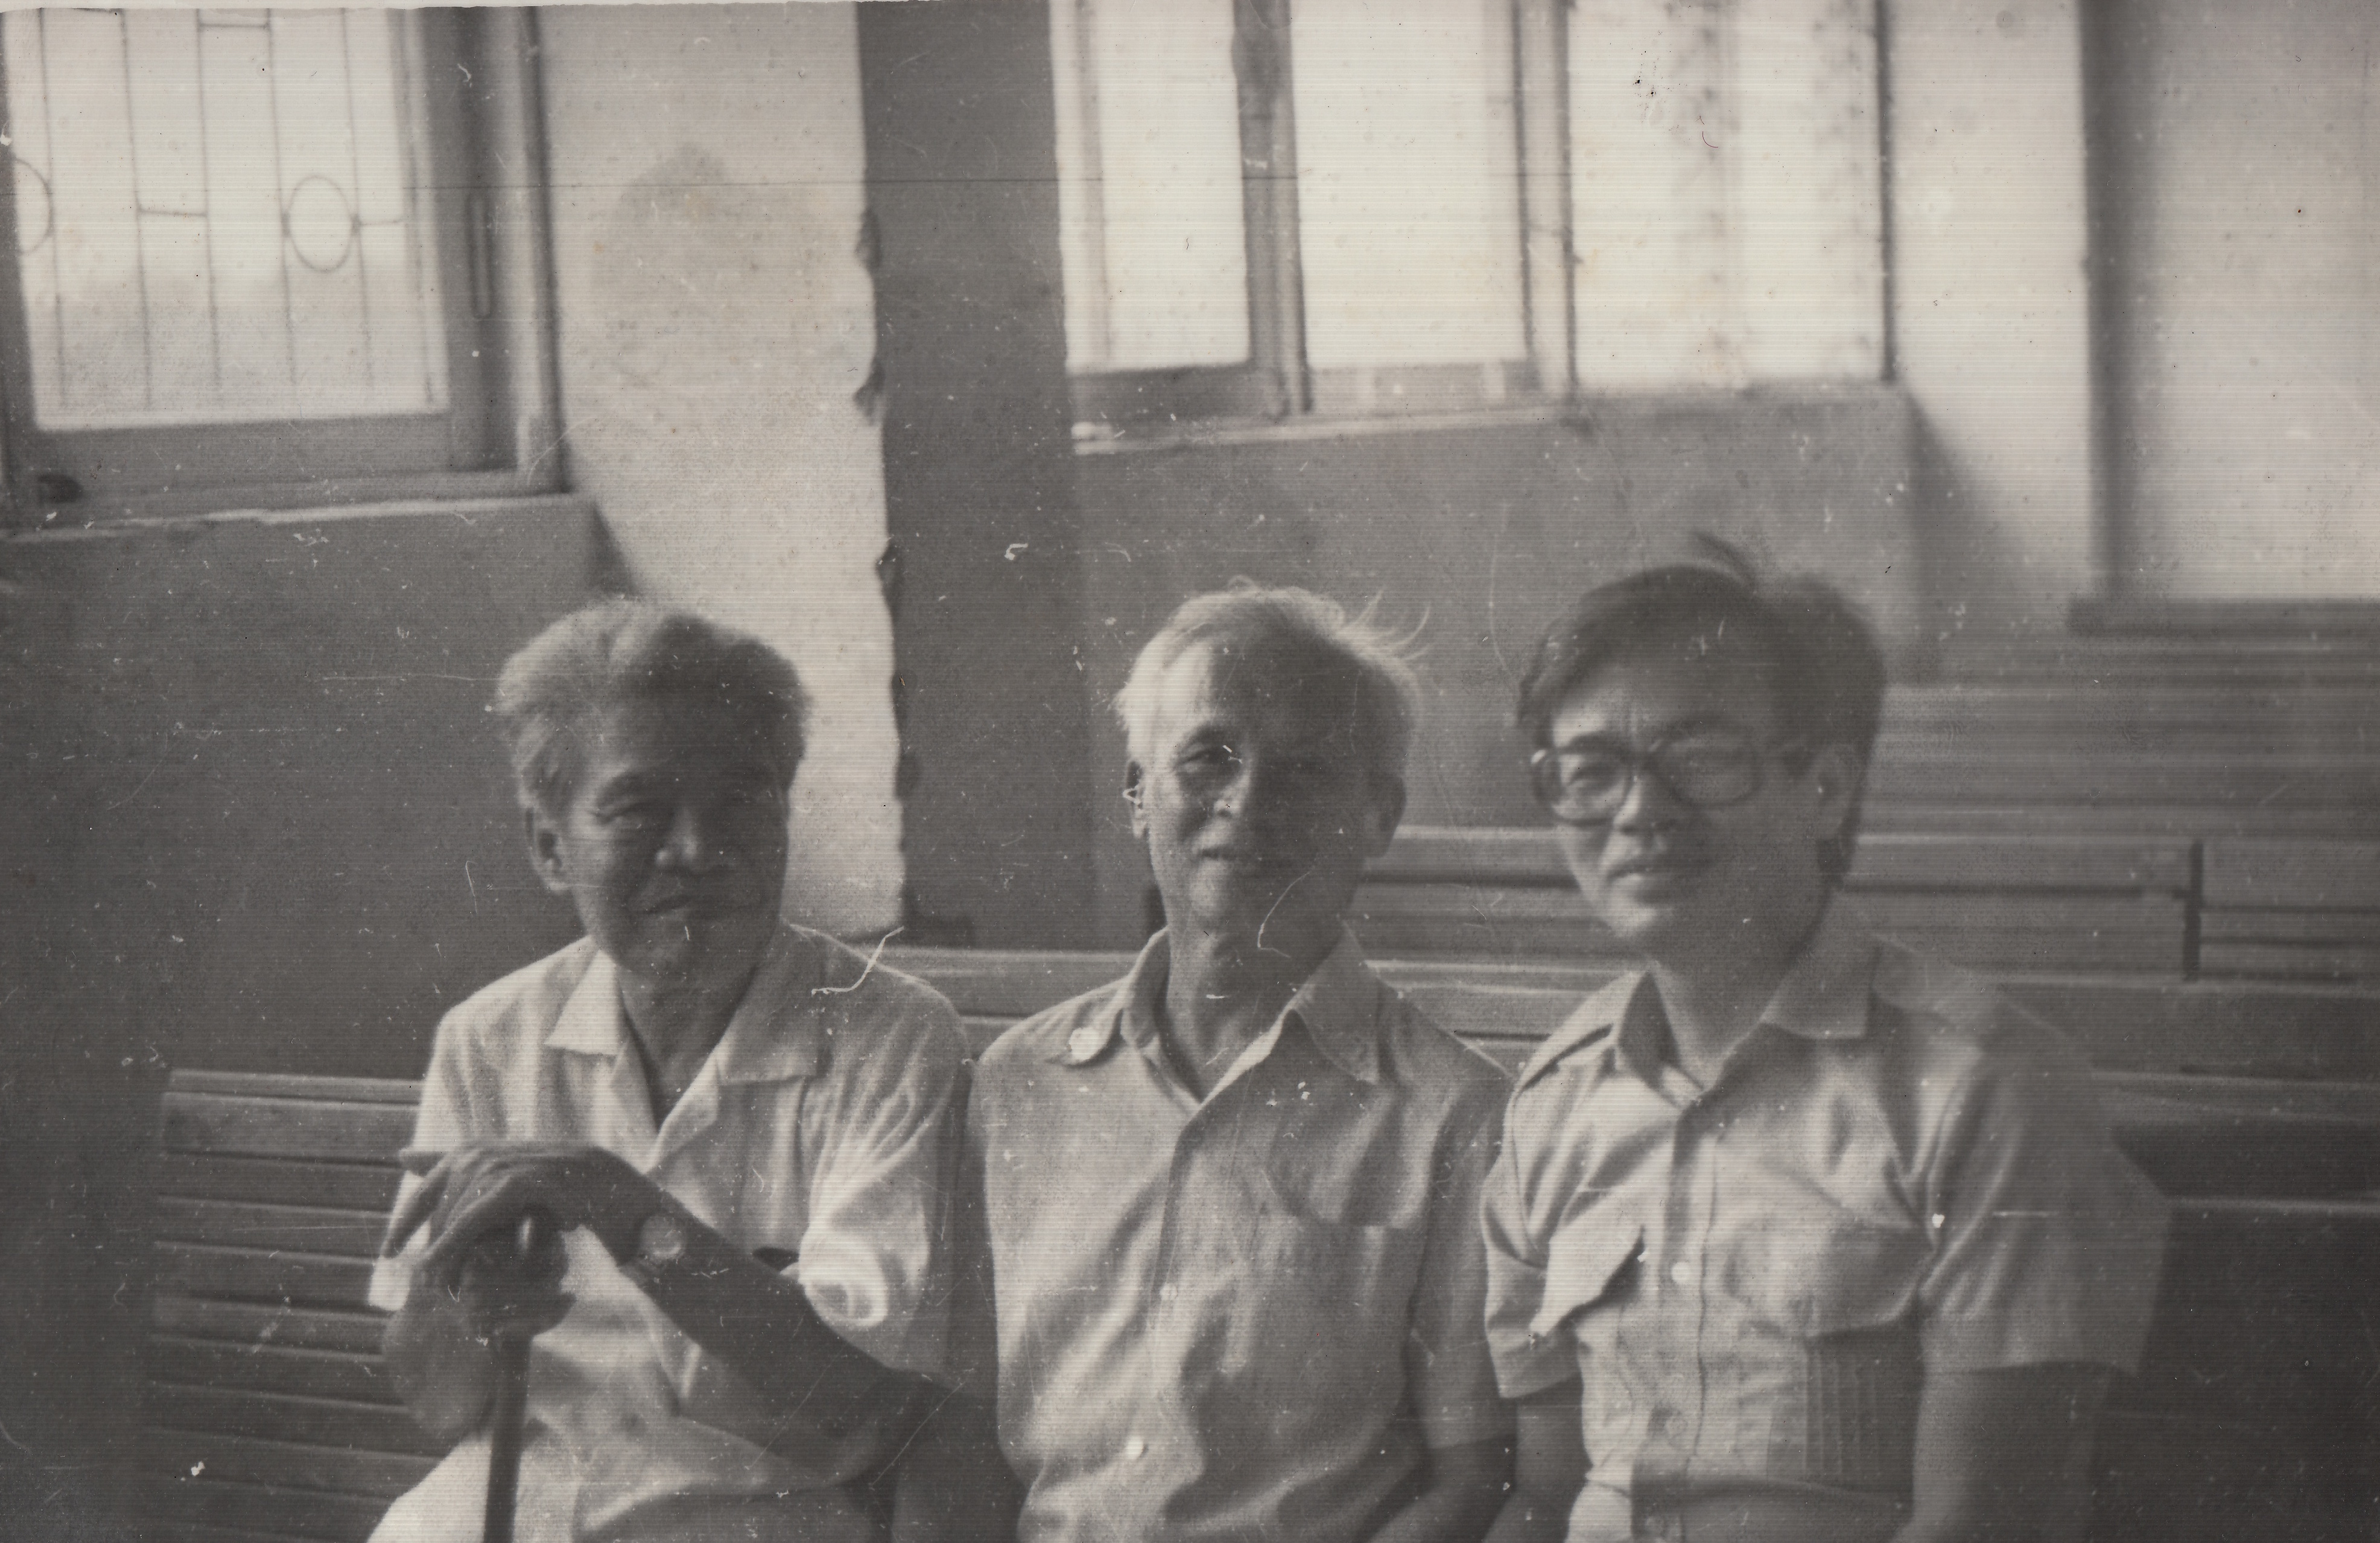
\includegraphics[scale=.075]{TaQuangBuu_LeVanThiem_PhanDinhDieu_nhungnam80}
     \caption{Tạ Quang Bửu, Lê Văn Thiêm và Phan Đình Diệu}
    \end{center}
    \end{figure}
\end{center}

Có một thói quen, không hiểu đã có từ bao giờ nhưng tôi nhớ đã được thừa hưởng từ những ngày kháng chiến chống Pháp, là gọi thầy giáo bằng “anh”, dù thầy có khi lớn hơn mình đến vài ba chục tuổi. Gọi bằng anh, một tiếng “Anh” đầy tôn kính mà thân tình. Rồi cách gọi Anh như vậy cũng được dùng cả với những người mà mình kính trọng, ngưỡng mộ, và may mắn có được chút quan hệ thân thiết tuy không phải là thầy dạy mình.  Tôi biết tiếng Giáo sư Tạ Quang Bửu, một nhà khoa học, một người hoạt động Nhà nước và xã hội nổi tiếng, từ khi mới là một học sinh Trung học ở quê nhà. Mãi đến cuối những năm 50, khi đã tốt nghiệp Đại học, đã đi dạy và bắt đầu tham gia chập chững vào con đường nghiên cứu khoa học, tôi mới được gặp Anh. Và, cũng như bao bạn khác, quên hết mọi xa cách về tuổi tác và cương vị công tác, chúng tôi đã gọi anh một cách hết sức tự nhiên là “Anh Bửu”.

	Hồi ấy, Anh đã về làm Hiệu trưởng Đại học Bách khoa Hà nội mới thành lập, rồi vài năm sau, làm Phó Chủ nhiệm kiêm Tổng thư ký Uỷ ban Khoa học nhà nước. Việc nước ta có một Uỷ ban Khoa học do những vị tài cao học rộng đầy uy tín (và cũng đầy huyền thoại) đứng đầu làm cho bọn trẻ chúng tôi hết sức háo hức, hăng hái tham gia mọi hoạt động do Uỷ ban tổ chức. Tôi dạy Toán ở Đại học Sư phạm, tham gia đều đặn các sinh hoạt xêmine Toán ở Uỷ ban. Một điều thú vị là tuy bận nhiều việc và quán xuyến nhiều ngành, nhưng Anh Bửu vẫn dành thì giờ tham gia chủ trì và thuyết giảng tại xêmine Toán về những vấn đề mới, có tính chất định hướng. Cho đến bây giờ tôi vẫn nhớ những buổi giảng của Anh, say sưa và sâu sắc, luôn hấp dẫn người nghe, hấp dẫn bởi cái say sưa nhiệt tình của người giảng là chính, dù người nghe chúng tôi nhiều khi chưa lĩnh hội được cái sâu sắc của bài giảng qua ngôn ngữ bác học của Anh. Đối với tôi, dù chưa hiểu bao nhiêu, nhưng tác động quan trọng của các bài giảng đó là gợi sự tò mò và lòng ham tìm hiểu; và rồi như sau này khi đã trải qua phần lớn cuộc đời mình, tôi nghiệm ra rằng cái hấp dẫn nhất đối với mình bao giờ cũng là cái chưa hiểu.

	Các bài giảng của Anh gây tác động nhiều nhất với tôi hồi đó là “Về các cấu trúc Bourbaki”. Sau khi tốt nghiệp rồi ra dạy học, mấy năm đầu tôi say mê học Lý thuyết số, rồi lan man từ các con số, do tò mò muốn hiểu cái gốc “tận cùng” của Toán học, vào những năm 1959-60, tôi bắt đầu tìm học Lôgích toán, Lý thuyết tập hợp, ... Tự học trong điều kiện tài liệu thiếu thốn, nên tôi chỉ hiểu lọ mọ thôi, nhiều cái không hiểu mà cứ tưởng là hiểu, hiểu sai mà cứ tưởng là hiểu đúng. Nghe Anh Bửu giảng các cấu trúc Bourbaki, tôi cũng chỉ hiểu lơ mơ, nhưng là những cái lơ mơ đầy hấp dẫn. Cho đến nay, tôi vẫn còn giữ được quyển sách nhỏ “Về các cấu trúc Bourbaki” của Anh. Quyển này, cũng tương tự như các quyển “Nguyên tử, hạt nhân, vũ trụ tuyến” và “Sống” mà Anh viết từ những năm 1947-48 trong chiến khu, có một nét chung là Anh muốn giới thiệu kịp thời, qua cách tóm lược cô đọng và súc tích của mình, những tư duy mới, những kết quả mới trong khoa học thế giới, nhằm giúp anh chị em khoa học trong nước tiếp cận nhanh với hiện đại. Không thể xem đó là những tài liệu phổ biến khoa học dễ hiểu. Với kiến thức sâu rộng của Anh, Anh có cách hiểu riêng để nắm bắt những điều cốt lõi trong các lý thuyết mới, và tôi nghĩ những điều Anh viết ra thường là những tiếp thu trí tuệ của Anh đối với các lý thuyết đó, do đó dễ hiểu với Anh mà khá khó hiểu với người khác. Nhưng tác động của những quyển sách nhỏ đó có lẽ chính là ở chỗ nó gây cho ta sự hấp dẫn say mê từ những hiểu biết lơ mơ luôn gợi trí tò mò. Từ tò mò đi đến tìm hiểu nghiêm túc, và rồi đến khi đã học tương đối thuần thục, trở lại đọc quyển sách nhỏ của Anh, ta sẽ có cái thú vị tìm được những đặc thù riêng trong cách cảm nhận của Anh mà trước đây ta chưa hiểu.

	Các cấu trúc Bourbaki, được xây dựng trên cơ sở lý thuyết tập hợp và lôgích cổ điển, là nền tảng để phát triển toàn bộ toán học, đó là niềm tin toán học ban đầu mà các bài giảng của Anh đã góp phần xác lập trong nhận thức của tôi. Nhưng rồi, niềm tin đó sớm bị lung lay. Hồi đó, tuy hiếm tài liệu, nhưng ham tìm thì rồi cũng có. Tôi say mê tìm các tài liệu “phê phán” toán học cổ điển, và thích thú đọc những hướng nghiên cứu xây dựng toán học theo các quan điểm lôgích, trực giác, kiến thiết,... Cũng nhờ đó, tôi đã được “hưởng” cái nhọc nhằn thú vị khi cố đọc cho hiểu định lý Gửdel với đầy đủ chứng minh tinh tế của nó . Có lần tôi mang những thắc mắc về quan niệm “đúng, sai” trong toán học hỏi ý kiến Anh, thì tôi biết được là tuy Anh thuyết giảng về Bourbaki, nhưng Anh cũng biết khá rành về các khuynh hướng khác, và anh nói với tôi về “cái đúng của Toán học phải tìm ngoài Toán học”. Vâng, và ngoài Toán học, cuộc đời còn biết bao công việc cần thiết khác. Sau này tôi được biết là hồi đó trong nhiều công việc quan trọng của Anh, có việc chuẩn bị gửi cán bộ ta sang thực tập nghiên cứu về máy tính và khoa học tính toán ở Liên Xô, nòng cốt để xây dựng ngành Tin học của ta sau này. 

	Chưa phải ngay từ những ngày đó tôi đã có thể lĩnh hội hết những điều được nghe Anh nói, nhưng rồi nhiều năm về sau, qua thực tế, tôi hiểu ra rằng Anh học nhiều về Toán với ý thức rõ rệt coi Toán học như một công cụ sắc bén của tư duy lôgích để từ đó tìm hiểu thấu đáo những vấn đề của nhiều lĩnh vực khoa học khác như vật lý, sinh học, khoa học điều khiển và quản lý, vân vân... , tức là tìm hiểu những thành tựu của khoa học hiện đại để định hướng cho việc xây dựng một nền giáo dục và nền khoa học kỹ thuật tiên tiến của đất nước. ý thức đó, cái ý thức gắn việc tìm hiểu khoa học hiện đại với kỳ vọng phát triển một nền giáo dục và khoa học tiên tiến cho nước nhà, có lẽ đã đeo đẳng mãi cho đến tận ngày Anh ra đi. 

	Cuối năm 1962, tôi được sang Liên Xô, làm nghiên cứu sinh tại Khoa Toán-Cơ, Đại học Tổng hợp Mạc tư khoa. Hồi đó, tôi “mê” toán học kiến thiết, một hướng toán học theo các quan điểm phê phán của phái “trực giác” nhưng được xây dựng trên cơ sở lý thuyết hiện đại về thuật toán, đang bắt đầu phát triển khá mạnh ở Liên Xô. Mê thì học thôi, chứ cái ý thức phục vụ xem chừng còn mơ hồ lắm. Rồi một lần, tôi nhận được thư Anh. Xúc động và bất ngờ, thư Anh viết thân tình như của một người Anh lớn, chứ không như của một cán bộ lãnh đạo. Tôi nhớ mãi câu “Cảm ơn các anh đang thực hiện những mơ ước của bản thân tôi...” Tôi hiểu trong đó vừa có sự gửi gắm, vừa có sự nhắc nhở. Và tôi dần có ý thức nhiều hơn về trách nhiệm đối với nơi đã gửi mình ra đi. Cũng vào thời gian đó, thầy giáo tôi, Giáo sư Markov, trước niềm đam mê hơi thái quá của đám học trò đối với cái toán học kiến thiết của ông, đã có một lời căn dặn hóm hỉnh mà tôi còn nhớ mãi: “Chúng ta có thể để cho trí tưởng tượng bay cao bao nhiêu cũng được, nhưng bao giờ cũng cần nhớ tìm con đường từ nơi cao ấy trở về mặt đất”. “Mặt đất” ấy của tôi là ở nơi đâu, tôi cũng bắt đầu nghĩ đến, và càng nghĩ càng thêm gắn bó.

	Khi bắt đầu có ý thức trách nhiệm đối với cái “mặt đất” của mình, một “mặt đất” còn lắm gian nan và nhiều thân thiết, thì cũng là lúc tôi suy nghĩ nhiều đến việc nên học cái gì. Học để thoả mãn trí tưởng tượng cũng là hay, nhưng là đâu con đường trở về “mặt đất” của mình? Và từ đây, tôi bắt đầu học được ở Anh một bài học mới, một bài học khó, mà hình như cho đến nay tôi vẫn chưa thể nào học được thuần thục. ấy là lần đầu tiên vào mùa thu năm 1965, sau khi làm xong cái phó tiến sĩ, tôi được bạn đề nghị cho ở lại thêm vài năm để làm tiếp luận văn tiến sĩ. Làm tiếp, thì tức là tiếp tục với toán học kiến thiết! Mà trong những năm ấy, thế giới nở rộ bao nhiêu hướng nghiên cứu đầy hấp dẫn ngay trong lĩnh vực toán học: khoa học thông tin, khoa học hệ thống, các lý thuyết điều khiển, vân vân và vân vân... Và tôi cảm nhận được rằng các hướng khoa học này chắc là sẽ hữu ích cho cái “mặt đất” của mình hơn là toán học kiến thiết. Thế là tôi đề nghị xin không tiếp tục làm tiến sĩ, mà được dành thì giờ học thêm về các khoa học đó. Và bất ngờ thay, tôi được Sứ quán chuyển đến chỉ thị trả lời của Anh: phải tiếp tục làm xong tiến sĩ, rồi sau hãy hay. Sau là thế nào? Cuối năm 1967, bảo vệ luận văn tiến sĩ xong, tôi về nước, đến chào Anh, Anh chỉ cười, bảo: Đấy, bây giờ muốn học thêm cái gì thì học. Anh không giải thích gì thêm, mãi về sau tình cờ tôi mới hiểu được ý Anh: Anh muốn tôi có thêm chút vốn liếng để dễ được cuộc đời chấp nhận hơn, và do đó mới có cơ hội làm được việc có ích hơn. 

	Muốn có ích cho đời, thì ngoài năng lực ra, cần phải được đời chấp nhận, bài học đó khi ngầm khi rõ, tôi đã được tiếp thụ ở Anh, không phải bằng thuyết giảng, mà bằng cách xử sự, bằng thiện chí, và cả bằng những cảm nhận không lời trong suốt nhiều năm về sau, thời gian mà may mắn tôi có cơ hội được gần Anh hơn. Tôi nhớ một chuyện vào đầu những năm 70. Hồi đó có một học sinh trẻ, tên là N., đến tìm tôi hỏi chuyện học. Sau vài lần kiểm tra, tôi ngạc nhiên thấy do không đi sơ tán nên đang học cấp 2 phải bỏ dở rồi chủ yếu là tự học lấy, mà chỉ trong vòng 3, 4 năm, em đã học xong cấp 3, tự học nhiều môn của chương trình đại học, đặc biệt nắm khá vững về giải tích, tôpô, và có thể nói là hiểu thấu đáo về lôgích toán. Em N. ở Hà nội với bà mẹ nuôi, còn bố mẹ đẻ làm nghề y, đã đi Nam từ 1954, khi em còn bé.  Tôi báo cáo với các thủ trưởng ở Uỷ ban Khoa học, nơi tôi công tác, với đề nghị được giúp đỡ. Sau vài lần đến gặp N. ở nhà tôi để cùng kiểm tra, một thủ trưởng hăng hái nói: có thể tuyển ngay vào Viện Toán rồi sẽ tạo điều kiện bồi dưỡng tiếp; thủ trưởng kia thận trọng hơn, vài hôm sau cho chỉ thị: không phí sức đào tạo những người như vậy. Tôi thất vọng tìm đến Anh, Anh hẹn gặp N. mấy lần, và sau đó bảo tôi: cái chuyện giúp N. giỏi Toán thì anh và tôi khỏi lo, tự nó sẽ giỏi, cái mà ta cần giúp là làm sao để cuộc đời chấp nhận nó. Và theo lời khuyên của Anh, N. thi vào năm thứ nhất Đại học, thi được điểm cao nhưng không được nhận học, tiếc là lúc đó Anh đi công tác xa nên chẳng biết kêu ai, năm sau lại kiên nhẫn thi một lần nữa, và nhờ có ý kiến của Anh nên được vào học, do học vượt nên tốt nghiệp sớm, nhưng rồi lần này thì tiếc thay, không sao làm được cho “cuộc đời chấp nhận”, chẳng cơ quan nào nhận N., và em phải ngậm ngùi ngơ ngẩn ra đi. 

	Bài học khó, tôi cố học, có thất bại và hình như cũng có lúc thành công. Và tôi hằng nghĩ trong việc thực hiện bài học này, Anh là một tấm gương lớn. Nhờ luôn tìm được lời giải đúng đắn cho bài học khó đó, mà Anh đã có những đóng góp to lớn tài năng và trí tuệ của mình vào sự nghiệp bảo vệ và xây dựng đất nước. Anh kính yêu, Anh đi xa rồi, có đôi lúc tôi muốn thầm hỏi Anh là trong suốt cuộc đời hoạt động sôi nổi của mình, đã có khi nào Anh có cảm giác bất lực trong việc tìm lời giải cho bài toán đó không Anh?  Tôi còn nhớ rõ, vào năm 1976, sau khi đất nước thống nhất, Anh làm việc hết sức hào hứng với chiến lược con người, đi Nam khảo sát nhiều ngày chuẩn bị cho kế hoạch phát triển giáo dục Đại học trong cả nước. Và rồi, trong phiên họp Quốc hội sau đó, cũng như nhiều đại biểu khác, tôi sững sờ biết tin Anh thôi làm Bộ trưởng Bộ Đại học. Vài tháng sau, trong một cuộc họp, Anh cho tôi xem một tài liệu đánh máy khá dày, là bản góp ý kiến phân tích một cách khoa học tính duy ý chí và không hiện thực của nhiều chỉ tiêu kinh tế xã hội trong một Dự thảo kế hoạch được trình ở một Đại hội quan trọng trước đó mấy tháng. Tôi không dám hỏi gì Anh thêm, và cũng không làm cái việc nối ghép các sự kiện.

	Một buổi sáng vào đầu những năm 80, trên con tàu từ Budapest sang Paris, ngồi một mình liên tưởng làm sao tôi lại buột nghĩ được hai câu thơ mở đầu cho một bài thơ mà từ lâu tôi có ý định làm tặng Anh:
\begin{center}
			Một khối nghĩ suy, một khối tình\\
			Nước non là đó, nọ là mình.
\end{center}
Rồi tắt ngấm, không thể nào nghĩ hơn được nữa, ngay lúc ấy và cả nhiều năm sau. Ngợi ca Anh ư? có thêm tôi thì cũng là thừa và biết đâu lại là vô duyên. Cho mãi đến sau khi Anh mất, một buổi chiều chở vợ đi chơi trên chiếc xe bé tí Peugeot 102, chiếc xe mà đã có lần tôi liều mạng chở Anh từ một cuộc họp về nhà do chờ ôtô của Bộ mà mãi không thấy đến đón, tôi miên man nghĩ đến Anh, có ý định nghĩ nốt cho trọn bài thơ còn bỏ dở. Lơ đãng thế nào để bánh xe kẹt vào đường ray tàu điện quãng phố Hàng Bột, cả hai vợ chồng ngã lăn ra đường. May không việc gì, lại lên xe đi tiếp. Và may mắn thay, sáu câu thơ đang thiếu bỗng chợt đến trong chốc lát. Tôi nhẩm nhớ, dở hay tôi không biết, có ý gì sái không và có điều gì không phải với Anh không, tôi chỉ còn biết mong được hương hồn Anh lượng thứ. Về nhà, tôi chép nắn nót những lời mộc mạc đó lên giấy, không gọt rũa gì thêm, vội mang đến nhà Anh đặt lên bàn thờ, rồi kính cẩn đọc dâng Anh . 

	Thế mà đã mười mấy năm rồi. Viết mấy dòng tưởng nhớ Anh, nghĩ đến công lao to lớn của Anh, đến những săn sóc thân tình mà bình sinh Anh luôn dành cho những em út đi sau một cách ân cần, ngẫm lại mình không mấy thành công trong việc tìm lời giải cho bài học khó học được từ Anh, tôi bất giác ngậm ngùi:
			\begin{center}
			Nước non là đó, nọ là mình....
			\end{center}
						\begin{flushright}
							Tháng 9 năm 1999\\
							  Phan Đình Diệu
							\end{flushright}

 
  %\includepdf[pages=1-,scale=0.85,pagecommand={\thispagestyle{plain}}]{Docs/1999_MotBaiHocKho(tangTQB).pdf}

\chapter{Trần Đại Nghĩa}\index{Trần Đại Nghĩa}
{\Large  TẶNG ANH}
		
Kính tặng Anh Trần Đại Nghĩa\\

	Nghĩa lớn gọi về với nước non\\
	Buồn vui đã trải cuộc vuông tròn\\
	Rèn tài văn võ thời phiêu bạt\\
	Gánh việc giang sơn thuở mất còn\\
	Tình nặng ấy chưng tình đất nước\\
	Nghiệp đời há kể nghiệp vàng son\\
	Gốc thông đứng thẳng dầu mưa nắng\\
	Để gió lành reo ngát nước non.\\

\chapter{Niềm ngưỡng mộ thầy Thiêm và tình yêu toán học (Lê Văn Thiêm)}\index{Lê Văn Thiêm}
%  \includepdf[pages=1-,noautoscale,pagecommand={\thispagestyle{plain}}]{Docs/xx_LeVanThiem.pdf}

 						\begin{flushright}
 						Tưởng nhớ Giáo sư Lê Văn Thiêm
 						\end{flushright}

	Tôi còn nhớ rõ lần đầu tiên tôi được nghe tiếng giáo sư Lê Văn Thiêm là vào một ngày đầu năm học 1948-1949, năm học trung học đầu tiên của tôi tại trường huyện (Can lộc, Hà tĩnh). Hôm ấy, thầy dạy Toán vào lớp, với một vẻ hân hoan hiếm có, kể cho chúng tôi nghe một tin tức từ báo chí ở Việt Bắc gửi về, trong đó có nói về một buổi nói chuyện của nhà khoa học Tạ Quang Bửu giới thiệu một số phát minh mới của khoa học thế giới, và giới thiệu thành tích của một số nhà khoa học Việt nam, đặc biệt về nhà toán học trẻ tuổi Lê Văn Thiêm, tiến sĩ Toán học đầu tiên của nước ta tại Pháp và hiện đang dạy học tại Thụy sĩ. Bọn học trò chúng tôi nghe một cách háo hức, để mà phấn khởi, tự hào, chứ thực ra chẳng hiểu gì mấy. Thế nào là một phát minh toán học, là một luận án tiến sĩ, làm thế nào mà một người Việt nam có thể nghĩ ra những "định lý toán học chưa ai từng biết"? Những câu hỏi như vậy thì trong nhiều năm sau chúng tôi vẫn chưa có câu trả lời, nhưng cái tên Lê Văn Thiêm, cùng với tên tuổi của các nhà khoa học cùng quê hương Nghệ Tĩnh như Hoàng Xuân Hãn, Tạ Quang  Bửu,... thì đã in đậm trong trí nhớ non nớt của chúng tôi, như những thần tượng, những mơ ước xa xôi mà thân thiết.  Trong thời thơ ấu ở một vùng quê heo hút, chính niềm ngưỡng mộ đối với những tên tuổi huyền thoại đó đã nhen nhóm trong lòng tôi niềm mê say toán học tự lúc nào mình cũng không biết.  

	Cho đến đầu năm 1955, khi từ quê ra thủ đô Hà nội mới được giải phóng để thi vào học Đại học, tôi mới có cơ hội tiếp cận với khả năng đạt được mong ước học Toán của mình. Nhưng chưa phải đã đạt được ngay mà còn phải trải qua một chặng thử thách khá trớ trêu nữa. Số là tôi ra Hà nội chậm mất vài ba ngày, không kịp dự thi vào Khoa Toán (Đại học Sư phạm) nữa, chỉ còn có thể thi vào các ngành như Dược, Sinh-Lý-Hóa (có thể xem là Dự bị Y khoa), và thế là năm học đầu tiên đó, tôi theo học Dược được vài tuần rồi học Sinh-Lý-Hóa cho đến hết năm học. Nhưng không dứt được lòng ham mê Toán học, thỉnh thoảng tôi vẫn đi nghe trộm (hay xem trộm) các buổi giảng ở lớp Toán, chẳng hiểu gì nhưng vẫn thích thú và bị cuốn hút bởi những điều lạ tai về vi phân, tích phân, ..., nên đến năm học sau, tôi đã bỏ việc theo học ngành Y và thi lại vào ngành Toán Đại học Sư phạm để được học Toán như ước muốn.

	Mấy năm học Toán ở Đại học Sư phạm Hà nội hồi ấy, tuy nhà trường còn nhiều thiếu thốn, nhưng đã là những năm học hành rất hào hứng đối với tuổi trẻ của tôi. Môn học nào cũng là mới mẻ, đầy hứng thú, chúng tôi được học với các thầy có uy tín, nhiều nhiệt tình. Thầy Thiêm dạy chúng tôi ở năm thứ ba, môn học Lý thuyết hàm số phức. Môn học được xem là khó, nhưng đầy hấp dẫn với những kiến thức mới lạ, những kết quả bất ngờ và những ứng dụng kỳ thú trong các lĩnh vực khác. Tôi nhớ, trong chương trình học hồi đó tôi thích nhất là các môn Cơ sở hình học, Số học và Lý thuyết hàm số phức, đặc biệt là những ứng dụng hàm số phức trong số học. Sau khi tốt nghiệp, ra trường được giữ lại dạy học ở khoa Toán, được bắt đầu một thời kỳ làm việc dưới sự chỉ đạo chung của thầy Thiêm, tôi đã chọn môn học đầu tiên mà mình nghiên cứu là Số học. Thầy Thiêm đã đồng ý với sự lựa chọn của tôi, và khuyến khích tôi đi sâu vào môn Số học. Thầy chỉ cho tôi biết những liên hệ thú vị giữa Lý thuyết hàm số phức và Số học. Số học là môn nghiên cứu về các con số, đã có lịch sử từ hơn hai nghìn năm và còn để lại biết bao bài toán khó nổi tiếng, lý thuyết hàm số phức nghiên cứu về các hàm số mà cả đối số và hàm số đều nhận giá trị là các số phức, tức chủ yếu là các số ảo, môn nghiên cứu tương đối mới mà thầy đã có nhiều kết quả đặc sắc, riêng những lý do đó dã hấp dẫn lòng say mê tuổi trẻ của tôi. Hồi đó, sách báo nghiên cứu khoa học ở nước ta còn rất thiếu thốn, nhưng may mắn làm sao tôi lại tìm mua được ở hiệu sách Tràng Tiền quyển "Số luận đạo dẫn" của Hoa La Canh mới xuất bản ở Bắc kinh, chỉ có điều là sách in bằng tiếng Trung quốc. Tôi cầm sách đến hỏi ý kiến thầy với băn khoăn là mình không biết đọc tiếng Trung quốc. Thầy mừng, bảo tôi: tìm được sách là tốt, Hoa La Canh là một nhà toán học lớn, nội dung sách rất hiện đại, còn chưa biết đọc tiếng Trung quốc thì phải cố học mà đọc cho được thôi. Thật là đơn giản, cái gì chưa biết mà cần biết thì phải cố mà học thôi, không được lùi bước; đó là bài học lớn đầu tiên tôi học được từ thầy. Tôi còn nhớ võ vẽ một ít chữ Hán học từ thuở bé, nay mua thêm một cuốn từ điển Hán-Việt của Văn Tân, rồi cố đọc sách của ông Hoa theo kiểu tra, đọc từng chữ Hán suốt một năm trời, cuối cùng cũng đọc được, hiểu được và dịch xong sách. Phần thưởng cho sự cố gắng đó là niềm hạnh phúc được hiểu biết những tri thức kỳ diệu về các con số, và đặc biệt nữa là về sự liên kết tài tình giữa các bộ môn khác nhau để tạo nên những điều kỳ diệu đó. Tôi bắt đầu hiểu đôi chút về Toán học và sự sáng tạo trong Toán học. Khảo sát về những vấn đề của lý thuyết hàm phức như các không điểm của hàm zêta $\zeta$ Riemann, dáng điệu của các tổng lượng giác,... mà lại có thể tìm ra phân bố các số nguyên tố, tìm các hướng đi nhằm giải quyết các bài toán khó trong số học như các bài toán Waring, Goldbach, v.v... Tôi còn được học với thầy Thiêm một chuyên đề nữa về Lý thuyết hàm số phức vào những năm đầu dạy học ở Đại học Sư phạm, đó là chuyên đề về ứng dụng trong các phương trình vi phân đạo hàm riêng. Chân trời liên kết giữa các ngành tri thức ngay trong một lĩnh vực Toán học trước mắt tôi đã được mở rộng và hiện ra thật sáng sủa, có tác động rất lớn trong việc hình thành nhận thức về khoa học sau này của tôi. Vào những năm 1958-60, ta bắt đầu có "phong trào" ứng dụng khoa học vào thực tế sản xuất và đời sống.  Tôi nhớ, hồi ấy các bậc đàn anh như thầy Thiêm với "bài toán thấm trong các công trình thủy lợi", anh Tụy với việc "ứng dụng Vận trù học", đã hăng hái đề xuất và dẫn đầu bọn trẻ chúng tôi đi vào thực tế, tìm kiếm các bài toán trong sản xuất nông nghiệp, trong thủy lợi, giao thông vận tải,...để ứng dụng Toán học; và chúng tôi, với ít hiểu biết và nhiều nhiệt tình, háo hức đi theo các anh về các nhà máy, hợp tác xã; kết quả của việc hăng hái "ứng dụng Toán học" thì có thể chưa có gì đáng kể, nhưng một ý thức gắn liền việc học lý thuyết với ứng dụng trong thực tế thì đã được hình thành đậm nét từ đó.  Với tôi, chính cái ý thức có vẻ còn mơ hồ từ thuở ấy đã dẫn dắt tôi đến với Tin học, Điều khiển học và Khoa học hệ thống sau này. Hình ảnh của thầy Thiêm, một nhà toán học lý thuyết lớn, một tiến sĩ Tây học, trong bộ quần áo giản dị, băng đồng lội ruộng, hăng hái một cách hồn nhiên trong những đợt đi thực tế, mãi mãi đối với tôi vẫn là hình ảnh thân thương về một tấm gương lớn của một nhà khoa học đàn anh trong niềm tin "khoa học phục vụ đời sống" của mình.

	Thời gian tôi được làm việc gần gũi với thầy Thiêm lâu nhất là từ khi thầy về công tác ở Viện Khoa học Việt nam, trực tiếp phụ trách xây dựng và phát triển Viện Toán học. Viện Toán học được chính thức thành lập từ đầu những năm 1970, lúc đầu chỉ có 4 bộ môn (Giải tích toán học, Vận trù học và Tối ưu hóa, Xác suất và thống kê, Lôgich và lý thuyết ôtômat), và đã trải qua một thời gian đầu xây dựng với nhiều thiếu thốn, khó khăn. Tuy nhiên, với ưu thế là một cơ sở nghiên cứu Toán học đầu tiên của cả nước, với uy tín khoa học của thầy Thiêm và của các nhà toán học đàn anh như GS Hoàng Tụy, Viện Toán đã nhanh chóng trở thành một địa chỉ tập trung đầy hấp dẫn đối với giới Toán học, sau một số năm đã thu hút được nhiều cán bộ nghiên cứu trẻ và có năng lực về công tác tại Viện. Viện đã sớm tạo được một không khí học thuật và nghiên cứu khoa học sôi nổi, phát triển và mở rộng công tác đào tạo và nghiên cứu ra hầu khắp các lĩnh vực toán học hiện đại, xuất bản đều đặn các tạp chí khoa học ở trình độ tiên tiến, có nhiều quan hệ hợp tác quốc tế rộng rãi,.... Là một cán bộ toán học, có may mắn được công tác một thời gian đầu ở Viện Toán dưới sự lãnh đạo chung của thầy Thiêm, về sau tuy không còn là thành viên của Viện nhưng vẫn nhiều gắn bó với Viện, tôi vẫn luôn xem Viện là "quê hương" của mình, và vui mừng nhận thấy trong không khí hoạt động sôi nổi và thân thiện, nhiều chất trí tuệ mà vẫn rất bình dị hiền hòa ngày nay của Viện, đâu đó vẫn phảng phất phong thái của vị Viện trưởng đầu tiên, của người thầy chung của giới Toán học, cố Giáo sư Lê Văn Thiêm kính yêu.  Tôi có vinh dự là người cùng quê Hà tĩnh với thầy Thiêm, tình yêu Toán học đã được nhen nhúm từ niềm ngưỡng mộ đối với thầy từ thuở thiếu thời, và cho đến nay, niềm ngưỡng mộ đó vẫn tiếp tục nuôi dưỡng tình yêu Toán học trong tôi, và tôi hiểu rằng nhiều niềm yêu khoa học khác mà tôi có được trong cuộc đời cũng đã được bắt nguồn từ chính tình yêu Toán học đó. 

								\begin{flushright}
								Phan Đình Diệu
								\end{flushright}




\chapter{Một Tấm Lòng Bao Dung Nhân Hậu (về Phạm Văn Đồng)}\index{Phạm Văn Đồng}
\label{chap:PVD}
 % \includepdf[pages=1-,noautoscale,pagecommand={\thispagestyle{plain}}]{Docs/2001_Mottamlongbaodungnhanhau(vePVD).pdf}

                                              MỘT TẤM LÒNG BAO DUNG NHÂN HẬU
                                                                                  Tưởng nhớ cố thủ tướng Phạm Văn Đồng
     Một trưa hè 1999 đang ngồi làm việc tôi bỗng nhận được đện thoại của anh Năng từ Tam Đảo gọi về.Anh Năng bảo tôi là “anh Tô nói chuyện với anh”.Liền đó tôi nghe từ xa giọng nói sang sảng quen thuộc của Thủ tương Phạm Văn Đồng bảo tôi nếu sắp xếp được thì lên Tam Đảo nghỉ dăm ba ngày và anh muốn trao đổi ý kiến về bài “Xã hội tri thức…” mà tôi vừa mới viết và có gửi biếu anh. Sáng hôm sau tôi lên nhà nghỉ Tam Đảo, làm việc với anh suốt buổi chiều, Anh hỏi, tôi trình bày ý kiến, Anh  gợi ý nên tìm hiểu sâu thêm  một số điểm, đặc biệt về “con đường hội nhập của chúng ta”. Anh đã 94 tuổi rồi mà vẫn minh mẫn, nói năng mạch lạc, chuyện trò vui vẻ. Tôi mừng thấy Anh vẫn khỏe mạnh. Hết giờ làm việc, tôi xin phép Anh về Hà Nội ,rất tiếc không ở lại thêm được  vì còn bận dạy học.Anh bắt tay tiễn tôi và bảo: Nếu trong hè còn lúc nào rỗi thì lên đây nghỉ, còn không đến tháng  9 Anh cũng về Hà Nội và rồi sẽ gặp nhau để “tiếp tục câu chuyện”. Tôi  nắm chặt tay Anh  và tin chắc là sẽ sớm  được gặp lại Anh. Có ngờ  đâu lần gặp Anh chiều hè ấy đã là lần gặp cuối cùng. Tháng 9 Anh về Hà Nội, bị mệt vào bệnh viện,  rồi từ đó Anh đã mãi mãi ra đi. Hôm viếng Anh, khi đi qua linh cữu, tôi thầm nói lời vĩnh biệt, kính chúc hương  hồn Anh thanh thản sau khi đã trút bỏ lại đằng sau bao lo toan vất vả suốt cuộc đời.
    Tôi là một cán bộ khoa học bình thường, vốn chỉ quen học Toán và dạy Toán. Một kỷ niệm sâu sắc trong đời sinh viên của tôi vào dịp lễ tốt nghiệp đại học sư phạm Hà nội năm 1957, tôi được Thủ tướng trao bằng khen, và trong bài phát biểu với những lời căn dặn chân tình của Anh hôm đó tôi còn ghi nhớ mãi hai chữ: cống hiến và trung thực. Vào dầu những năm 60, khi có điều kiện được làm nghiên cứu khoa học ở Đại học Mạc tư khoa, tôi vẫn mê Toán học trừu tượng, nhưng đồng thời cũng suy ngẫm rất nhiều về chữ cống hiến, mình là một cán bộ khoa học ở nước nghèo, liệu có thể hoc được cái gì có ích trực tiếp hơn chút ít hay không. Thời ấy, máy tính đang bắt đầu được phát triển mạnh, và các khoa học về thông tin, điều khiển đã ra đời với nhiều ý tưởng mới, nhiều triển vọng ứng dụng mới. Vì thế là, cùng với việc lo hoàn thành luận văn về Toán, tôi bắt đầu say mê với công việc tìm hiểu các nghành khoa học mới đó. Sau khi về nước, được Anh gọi đến mời cơm và trò truyện, tôi có dè dặt trình bày với Anh một vài suy nghĩ và dự định, và rất vui mừng được Anh khích lệ.
    Tôi biết rằng Anh cũng như nhiều vị lãnh đạo thuở ấy, vốn là những trí thức lỗi lạc, hiểu rất rõ tầm quan trọng của khoa học kỹ thuật đối với việc phát triển đất nước, nên hết sức chăm lo xây dựng nền khoa học và kỹ thuật còn rất non trẻ của nước nhà. Và anh chị em khoa học kỹ thuật của chúng ta hồi đó, tuy chưa đông và còn ít kinh nghiệm, nhưng với nhiệt tình trong sáng luôn sãn sàng tìm đến những vấn đề thực tiễn trong sản xuất và đời sống để mong muốn được đóng góp. Ứng dụng Toán học, rồi tiếp đó với việc sử dụng máy tính  điện tử, là một lĩnh vực bắt đầu được sự quan tâm chú ý của xã hội. Nhờ những cố gắng không mệt mỏi và đầy say mê của lớp các nhà toán học đàn anh, một không khí ứng dụng Toán học,vận trù học,… đã có những lúc khá sôi nổi trong những năm 60, 70, kéo theo một giai đoạn hào hứng và có nhiều kết quả trong các hoạt động đào tạo và nghiên cứu Toán học, và tiếp theo là tin học, ở nước ta. Vào cuối những năm 60 của thập niên 70, tôi cũng thỉnh thoảng được Anh gọi đến trò chuyện thân mật, trao đổi ý kiến, khuyến khích các nghiên cứu ứng dụng toán học và máy tính điện tử. Có một điều thú vị mà tôi hết sức chú ý là Anh không chỉ khuyến khích, động viên một cách chung chung, mà thực sự Anh rất quan tâm đến những quan đểm mới của các khoa học về hệ thống, về thông tin và điều khiển, đặc biệt đến khả năng ứng dụng các khoa học đó vào việc cải tến tổ chức và quản lý kinh tế, xã hội. Chính với sự quan tâm có chiều sâu tư duy đó mà vào đầu những năm 70, khi tình hình chiến tranh còn rất ác liệt, Anh đẫ chỉ thị nghiên cứu chuẩn bị, và sau đó đã ký ban hành hai Nghị quyết của Chính phủ về “Đẩy mạnh ứng dụng Toán học và máy tính trong công tác quản lý kinh tế” (1975) và “Xây dựng và phát triển ngành khoa học tính toán ở nước ta” (1976) với những nội dung và biện pháp tổ chức thực hiện tương đôi toàn diện, cụ thể và thiết thực. Vào thời gian đó, chưa có Chính phủ nào trong khu vực chúng ta có những chủ trương và chính sách tích cự, rõ ràng như vậy về việc phát triển Toán học và Tin học. Tiếc rằng về sau, các Nghị quyết sáng suốt và tích cực đó đã không được chỉ đạo thực hiện một cách nghiêm túc và nhất quán, nên kết quả đã có nhiều hạn chế như chúng ta thấy hiện nay.
    Những năm sau khi thống nhất đất nước, phát triển kinh tế là nhiệm vụ trọng tâm, và cải tiến quản lý kinh tế nhanh chóng chở thành yêu cầu bức thiết và cấp bách nhất của đất nước. Là một cán bộ khoa học được giao nhiệm vụ Viện trưởng Viện Khoa học tính toán và điều khiển, lại là đại biểu Quốc hội, tôi cũng suy nghĩ nhiều về tình hình đất nước sau chiến tranh, về khả năng ứng dụng khoa học để đóng góp vào việc cải tiến tổ chức và quản lý kinh tế,…, và do đó trong một vài kỳ họp của Quốc hội, đặc biệt cuộc cuối năm 1980, tôi đã mạnh dạn tham luận về yêu cầu đổi mới một số chính sách phát triển kinh tế và đề nghị bắt đầu ứng dụng tin học vào quản lý. Bài thảo luận có một số ý kiến khác với những suy nghĩ chung hồi đó, nên có người không tán thành. Tôi nhớ sau kỳ họp vài tuần Anh có gọi tôi đến trao đổi hồi lâu, rồi anh bảo: Tôi biết là tham luận chỉ trình bày được ngắn, nhưng chắc anh có nhiều suy nghĩ, đề nghị anh về suy nghĩ kỹ thêm và viết thành bài nghiên cứu cho tôi xem. Theo chỉ thị của Anh, về nhà tôi hào hứng suy nghĩ, nghiên cứu thêm, và khoảng ba tháng sau, tôi gửi trình Anh bài nghiên cứu “Khoa học hệ thống và một số ý kiến về vấn đề cải tiến quản lý kinh tế hiện nay”. Bài dày 46 trang đánh máy, có thể có hay, dở, đúng, sai, nhưng đó là bài viết tâm huyết đầu tiên của tôi về sự phát triển đất nước; khi viết thì các ý cứ được rút ra theo mạch logic của tư duy, nhưng viết xong đọc lại thì mới chợt nhận ra có khá nhiều ý kiến không phù hợp với các chủ trương chính thức. Nhưng rồi tôi vẫn gửi đi, vì tôi muốn báo cáo với Anh những suy nghĩ ‘‘trung thực’’ của một cán bộ khoa học. Cùng gửi cho Anh, tôi có gửi đến hai vị lãnh đạo trực tiếp nữa. Rồi chờ đợi những lời phê phán. Quả thực, một tuần sau, một vị cho truyền đến một chỉ thị; tuyệt đối không được phổ biến ra ngoài những tư tưởng của bài viết. Tôi chấp hành chỉ thị, nhưng vẫn huy vọng nhận được  ý kiến của Anh. Mấy tuần sau, tôi đánh bạo gọi điện đến văn phòng của Anh để hỏi, thì được anh Hoàng Quốc Dũng, thư ký của Anh, vui vẻ trả lời: “anh yên tâm, anh Tô đã xem mấy lần, và nay bài viết của anh đang ở đây, anh Tô bảo tôi tham khảo để chuẩn bị cho một phát biểu sắp tới của anh ấy”. Tôi mừng, vì tôi chắc chắn Anh không tán thành nhiều ý kiến của tôi, nhưng Anh chấp nhận xem xét cả những ý kiến trái chiều như vậy một cách thông cảm và tôn trọng như vậy. Riêng ý nghĩ đó đối với tôi đã là một niềm khích lệ lớn.
    Sau lần đó, trong suốt hai thập niên 80 và 90, tôi còn có nhiều dịp được hưởng sự khích lệ đầy thông cảm của Anh trong những suy nghĩ và những công việc của mình. Chẳng hạn, đầu năm 1991, tôi trình bản “Kiến nghị về một chương trình cấp bách nhằm khắc phục khủng hoảng và tạo điều kiện lành mạnh cho sự phát triển đất nước”, trong khi bản kiến nghị đang bị phê phán thì Anh cho tổ chức liền hai buổi họp với một số ít anh em khoa học cả về khoa học tự nhiên và khoa học xã hội để cho tôi trình bày nội dung bản kiến nghị và trao đổi ý kiến một cách thân mật thẳng thắn; tôi không dám xem Kiến nghị là những điều phải theo, nhưng dẫu sao đó là suy nghĩ tâm huyết của một công dân, cách sử sự công bằng, thiện chí và đầy lòng thông cảm của Anh là một sự động viên rất lớn đối với bản thân tôi. Tôi tự biết rằng tôi không có khả năng đóng góp gì lớn, nhưng với tư cách một công dân, một cán bộ khoa học, tôi vẫn thường xuyên học hỏi những quan điểm mới trong tư duy khoa học hiện đại và cố vận dụng để tìm hiểu những vấn đề thực chất của sự phát triển đất nước, và tôi lấy làm may mắn là thường được Anh gọi đến để trình bày với Anh, nghe những gợi ý của Anh, và quan trọng hơn nữa là được khuyến khích bởi sự thấu hiểu và những niềm cảm thông thân thiết của Anh.  
       Lần cuối cùng gặp anh ở nhà nghỉ Tam Đảo, trước khi ra về, tôi có xúc động nhắc lại với Anh là tôi không ngờ lời dặn (có thể là bình thường) của Anh đối với lớp sinh viên Sư phạm tốt nghiệp năm 1957 về cống hiến và trung thực đã đi theo tôi gần trọn cuộc đời; cống hiến thì tôi chẳng làm được gì nhiều vì năng lực ít và cơ hội thành công lại càng ít hơn, nhưng trung thực thì tôi cố giữ đến trọn đời. Anh nắm trặt tay tôi và bảo; có lẽ bây giờ trung thực phải đặt lên trước vì là cái thiếu nhất. Đã không bao giờ còn những buổi chiều được trò chuyện với Anh trong không khí thanh bình, yên ổn, trong bình dị và cảm thông, nhưng tôi biết là tôi sẽ còn giữ mãi hình ảnh kính yêu của Anh, hình ảnh của một con người đầy bao dung và nhân hậu.
                                                                                           Tháng năm, năm 2001
                                                                                              Phan Đình Diệu   

1.	Anh Năng là thư ký riêng của cố thủ tướng Phạm Văn Đồng.
2.	Đó là bài “hướng tới thế kỷ 21: Xã hội tri thức và vài suy nghĩ về con đường hội nhập của chúng ta”, báo các tại Diễn đàn Công nghệ thông tin 1999 tại Thành phố Hồ Chí Minh, có đăng trong Xã hội học, số 2(66), 1999 và một số tạp trí khác.
3.	Tôi xin được nói một chút về cách xưng hô. Gọi Thủ tướng, người có tuổi bậc cha mình, là anh thì quả thực có cái gì đó là vô lễ. Nhưng vì đã quen gọi Anh, một tiếng Anh đầy tôn kính và ngưỡng mộ, nên trong bài này tôi cũng xin phép gọi như đã từng quen gọi, mong được bạn đọc thông cảm.


\chapter{Niềm Kính Yêu Đối Với Người Thầy Mẫu Mực (Nguyễn Thức Hào)}\index{Nguyễn Thức Hào}

  %\includepdf[pages=1-,noautoscale,pagecommand={\thispagestyle{plain}}]{Docs/xx_NguyenThucHao.pdf}

\begin{center}
      \textit{Kính tặng Giáo sư Nguyễn Thúc Hào nhân dịp mừng thọ Thầy 95 tuổi.}

      \end{center}      
      
      Tôi theo học ở Khoa Toán Đại học Sư phạm Hà nội vào khoá học 1955-
1957. Các bạn học cùng khoá thời đó, dù cách đây đã một nửa thế kỷ, nhưng vẫn
còn rất gắn bó với nhau, hàng năm vẫn họp mặt cùng nhau để hàn huyên về những
kỷ niệm cũ, những kỷ niệm của một thời tuy đã khá xa nhưng đối với mỗi chúng tôi
vẫn rất thân thương gần gũi. Trong những cuộc họp mặt hàng năm đó, các kỷ niệm
sâu sắc mà chúng tôi vẫn thường nhắc đến một cách đầy kính yêu và trân trọng là
về các thầy giáo yêu quí một thuở của mình. Điều may mắn đối với lớp học trò
chúng tôi ngày ấy là, tuy trong hoàn cảnh đất nước mới được hoà bình sau cuộc
kháng chiến chống Pháp, cuộc sống còn nhiều thiếu thốn, trường lớp mới được
phục hồi, v.v..., nhưng chúng tôi đã được học với các bậc thầy mà tài năng và đức
độ đã nổi tiếng làm chúng tôi rất ngưỡng mộ: đó là các thầy Lê Văn Thiêm,
Nguyễn Thúc Hào, Nguyễn Cảnh Toàn, Ngô Thúc Lanh, vân vân.

      Thầy Nguyễn Thúc Hào dạy cho khoá học chúng tôi hai môn học: môn Hình
học giải tích ở năm thứ nhất, và môn Hình học vi phân ở năm thứ ba. Thầy thuộc
lớp giáo sư đã có tuổi, đã từng dạy học nhiều năm ở Huế trước Cách mạng tháng
Tám, và trong những năm kháng chiến đã tự mình mở lớp dạy Đại học ở quê nhà
rồi sau đó tham gia xây dựng và giảng dạy các lớp đại học chính thức đầu tiên của
nước ta được mở ở Thanh hoá, ở Nam ninh (trên đất Trung quốc); thầy không
những nổi tiếng về dạy hay, dạy giỏi, mà còn rất nổi tiếng về tính nghiêm khắc và
mẫu mực trong công việc dạy học. Trong mấy năm được học với thầy qua hai môn
học khó về Hình học, chúng tôi đã được trực tiếp chứng kiến và thụ hưởng những
đức tính nói trên của người thầy mà mình rất đỗi ngưỡng mộ. Cho đến bây giờ, sau
khi đã trải qua cả một cuộc đời đi dạy học, chúng tôi vẫn còn nhớ như in những bài
giảng Toán của thầy với những hình vẽ thẳng ra thẳng, tròn ra tròn, ngay ngắn,
chính xác, với những nét chữ đẹp và đều đặn như chữ mẫu viết tập. Lời thầy giảng
bao giờ cũng rõ ràng, trong sáng, vừa đủ để giảng giải, để thuyết minh bài giảng,
gần như không thừa và cũng không thiếu, và bài giảng luôn luôn được thực hiện
đúng giờ, chẳng khi nào bị kéo dài quá giờ; nói tóm lại, mỗi tiết giảng của thầy bao
giờ cũng có thể được xem là một tiết giảng mẫu mực mà mãi về sau này, khi đã làm
thầy giáo, chúng tôi luôn cố gắng noi theo. Tất nhiên, tính mẫu mực bao giờ cũng
đi kèm với những yêu cầu nghiêm túc đối với người học. Tôi nhớ, thầy rất hiền từ,
không bao giờ nổi nóng với học trò, luôn nhẹ nhàng chỉ bảo những khi học trò
chúng tôi tỏ ra chậm hiểu, mà những điều “chậm hiểu” của lũ học trò chúng tôi thì
thường không phải là ít, có những điều phát biểu ra được nhưng cũng có nhiều điều
e ngại không dám nói ra, vì các bài học hình học của thầy thường là khó, đòi hỏi trí
tưởng tượng phong phú và cả những suy luận sắc sảo, và nhất là đòi hỏi người học
phải luôn tập trung chú ý nghe thầy giảng trong giờ học. Thực ra, thầy cũng không
đòi hỏi ở học trò chúng tôi những gì quá cao, cao hơn hẳn những chuẩn mực bình
thường, nhưng có thể vì chương trình học nói chung khá căng thẳng, nên đối với
các yêu cầu “bình thường” đó nhiều khi chúng tôi cũng chưa đáp ứng được, và vì
vậy các bài kiểm tra hoặc thi về các môn học của thầy, chúng tôi thường đạt được
điểm rất thấp, có lần gần như nửa lớp phải nhận điểm 0/10; cả đến kỳ thi tốt nghiệp,
đối với môn hình học vi phân, chỉ có khoảng 1/10 số học sinh trong lớp đạt được
điểm trên trung bình (5/10). Yêu cầu nghiêm khắc đối với việc tiếp thu kiến thức
của học sinh, và tính nghiêm túc, không dễ dãi trong việc đánh giá kết quả học tập
của người học là những kinh nghiệm quí mà về sau này khi đi dạy học, qua kinh
nghiệm thực tế, chúng tôi mới thấy là chỉ cần buông lỏng tinh thần trách nhiệm và
đạo đức nghề nghiệp của người thầy thì không dễ gì thực hiện nổi. Ngày nay, trong
công cuộc cải cách giáo dục, nhìn lại thực tiễn hoạt động giáo dục mấy chục năm
qua, chúng ta đã càng ngày càng thấy rõ một trong những yếu kém cần được khắc
phục của thực tế giáo dục ở mọi cấp học của ta là sự thiếu nghiêm túc trong cả việc
dạy và việc học: thầy dạy không ra dạy, trò học không ra học, thầy dạy tắc trách
trên trường lớp, còn dành phần kiến thức cho việc dạy thêm để kiếm tiền, học trò đi
học chẳng cần hiểu, bởi vì điểm cao, thi đậu,... có thể kiếm được bằng tiền mà
chẳng cần có kiến thức thật; không chỉ trong ngành giáo dục mà cả trong nhiều lĩnh
vực hoạt động khác, chính sự thiếu nghiêm túc, sự dối trá trong việc làm, sự dối trá
đặc biệt trong đánh giá, nhận xét, thẩm định,...đang là một căn bệnh gây nên biết
bao tiêu cực và thiệt hại cho xã hội ta. Cứ mỗi lần gặp một sự việc như vậy trong
cuộc sống hàng ngày, tôi lại nhớ đến người thầy mẫu mực của mình để mà suy
ngẫm, mà chiêm nghiệm, để càng thêm kính yêu, trân trọng những kỷ niệm về một
thời được học với thầy.

        Tôi chỉ là một học trò, được biết chút ít về thầy qua những năm học ở trường.
Về sau, khi ra trường, có dịp được tiếp xúc rộng hơn, tôi được nhiều bạn bè và
đồng nghiệp quen biết kể cho nghe nhiều câu chuyện cảm động khác trong cuộc đời
hoạt động của thầy, những câu chuyện luôn làm sâu đậm thêm trong ý thức của tôi
về hình ảnh một người thầy nghiêm túc mà gần gũi, một tấm gương về một nhà
giáo mẫu mực, tận tuỵ với nghề, tận tình với học trò, một thầy giáo có kiến thức
khoa học uyên thâm và vẫn đậm phong cách nhân ái của một ông đồ xứ Nghệ. Sau
khi tốt nghiệp ra trường, tôi được giữ lại làm cán bộ giảng dạy tại khoa Toán của
trường, được có cơ hội sống và làm việc cùng thầy thêm một thời gian nữa. Lúc ấy
thầy vẫn là Phó Hiệu trưởng trường Đại học Sư phạm Hà nội kiêm Chủ nhiệm
Khoa Toán. Mấy năm được công tác cùng khoa với thầy, các anh em cán bộ trẻ
chúng tôi có dịp được học tập rất nhiều ở thầy, học thêm về kiến thức chuyên môn
đã đành, nhưng quan trọng hơn là học được ở thầy về phương pháp giảng dạy, các
kinh nghiệm dạy học, từ việc soạn bài, chuẩn bị một bài giảng, cho đến việc trình
bày, giảng giải, hướng dẫn làm một bài tập, vân vân. Và bài học lớn nhất, thấm thía
nhất chúng tôi học được, dù không qua một buổi lên lớp nào cả, là lòng yêu nghề, ý
thức trách nhiệm nghề nghiệp, đạo đức và lòng tự trọng của một người thầy giáo,
tính nghiêm túc, kỷ luật, mẫu mực nhất thiết phải có đối với một người đã chọn dạy
học làm nghề nghiệp cho cuộc sống của mình.


	Cách đây hai mươi lăm năm, nhân mừng thọ 70 tuổi của thầy Hào, anh Văn
Như Cương, một bạn học cùng lớp thời đại học, có làm tặng thầy một bài thơ
đường luật, coi như bài thơ xướng và yêu cầu các bạn học làm thơ hoạ để cùng
mừng thọ thầy. Tôi nhớ bài thơ xướng của anh Văn Như Cương là như sau:

\begin{align*}
&\text{Mừng thầy nay thọ bảy mươi tròn}\\
&\text{Sáu nổi một chìm với nước non }\\
&\text{Tính toán một đời hai tay trắng}\\
&\text{Chắt chiu hai tốt một lòng son }
\end{align*}
	\begin{align*}
&\text{Lơ thơ lui tới trò và bạn }\\
&\text{Ríu rít ra vào cháu với con}\\
&\text{Dẫu biết bảy mươi xưa nay hiếm }\\
&\text{Vẫn mong thầy thọ đến trăm tròn. }
\end{align*}









	Tôi cũng nhớ là lần ấy, bản thân thầy Hào có làm một bài thơ tự vịnh rất hay,
gọi là để hoạ bài thơ của anh Cương. Hưởng ứng sáng kiến của ông bạn
V.N.Cương, tôi cũng có làm một bài hoạ để mừng thọ thầy, thơ chắc là còn rất
vụng, nhưng chỉ dám nói là cố theo đúng tinh thần nghiêm túc, trong trường hợp
này là đúng niêm đúng luật. Thơ như sau:
	
	\begin{align*}
	&\text{Một tấm gương trong giữ vẹn tròn}\\
	&\text{Sá bao công vượt suối trèo non}\\
	&\text{Tay dù trắng, đẹp đời trong trắng}\\
	&\text{Lòng vẫn son, bền chí sắt son.}
		\end{align*}
	\begin{align*}
	&\text{Từng trải nắng mưa lo nghiệp lớn}\\
	&\text{Giờ vui mây nước mảnh tình con}\\
	&\text{Đời còn sương bụi bao mờ tỏ}\\
	&\text{Xin mãi long lanh ánh nguyệt tròn.}
\end{align*}








					\begin{center}
					\textbf{Phan Đình Diệu}
					\end{center}

\chapter{Thơ}
  %\includepdf[pages=1-,noautoscale,pagecommand={\thispagestyle{plain}}]{Docs/xx_ThoBoDieu.pdf}  
%\part{Một Số Bài Viết Về Phan Đình Diệu }
%\clearpage{\pagestyle{empty}\cleardoublepage}

\begin{center}
\textbf{Nếu như em về đây} \\
(Hà Tĩnh, 1961)

Mưa nhẹ đường thôn gió vờn sóng lúa\\
Ôi xa rồi những ngày xưa êm ả\\
Những Tết xưa ấp ủ đợi chờ\\
Rảo bước đường quê nhớ tuổi  ấu thơ\\
Lòng man mác bao ước mơ vời vợi\\
Xóm cũ đây rồi làng xưa êm ái \\
Một bếp lửa hồng một tối đoàn viên \\
Một ý trẻ thơ mơ ước hão huyền \\
Ôi phút chốc cả sóng chiều xao động \\
Thức dậy vô vàn ước vọng xốn xang \\
Một bóng tre làng một bờ giếng ngọt \\
Phải chăng em là tươi mát tình em \\
Cả quê hương thân thiết êm đềm \\


Trên mái tóc em dịu mềm vương vấn\\
Trong đôi mắt em trời xanh thăm thắm \\
Trên môi em say đắm mặn mà \\
Kết lại giờ đây em hỡi, tình ta \\
Là em đó cả xa xưa sống lại \\
Cả hôm nay và mãi mãi mai sau \\
Như tiếng nói quê ta nghĩa nặng tình sâu \\

Đã đến đây rồi với bước cầu quen thuộc \\
Với mái nhà thân yêu \\
Có mẹ già anh sớm sớm chiều chiều \\
Ngóng đợi em về chắt chiu thương mến\\
Tấm lòng quê dù chẳng diễn thành lời \\
Trong khó nhọc vẫn ngời ngời hy vọng \\
Và bà anh phơ phơ tóc trắng \\
Tám chục tuổi tròn nghe tin em lòng bỗng hết héo hon \\
Hết ốm hết đau sức già trẻ lại\\
Xay lúa đêm đêm tay chờ tay đợi \\
Tấm lòng già khấp khởi thầm  mong \\
Và những đứa em thấp thỏm trong lòng\\
Chờ đón một tình thương gần gũi\\
Cả quê hương như êm đềm thân ái\\
Giang rộng tay mời đón bạn thương yêu \\
Trong lòng quê thanh bạch cảnh nghèo \\
Em yêu ơi! Nếu như em về đây...  


\end{center}
\newpage
\begin{center}
\textbf{Trên đường nhớ em}\\




	Nắng vàng Hà Nội trưa nay\\
Xa em kể tự phút này chia phôi\\
	Cầm tay nhau chẳng nỡ rời\\
Rưng rưng mắt lệ nghẹn lời chia ly\\
	Còi tàu vội giục chân đi\\
Buông tay ngơ ngẩn biết gì chăng em ?\\
	Dõi trông tay vẫy dịu mềm, \\
Bàng hoàng nào tưởng xa em, xa rồi.\\
	Nỗi tình ngày ngắn đêm vơi\\
Bâng khuâng cảnh mới, bồi hồi niềm xưa.\\
	Điều kia nửa tỏ nửa mờ\\
Lo âu để lại bây giờ một ai\\
	Nhớ thương trĩu nặng đường dài\\
Nhủ mình thôi cố rút ngày chờ mong.\\

		*
	
	Chiều hôm đất Lạng Đồng Đăng\\
Đường qua biên giới chập trùng núi cao.\\
	Nhìn quê mà dạ nôn nao\\
Vài dòng gửi lại biết nào tới em.\\

		*

	Dùng dằng chốc đã nửa đêm\\
Bằng Tường tàu đã sắp êm ghế ngồi.\\
	Nhớ về Hà Nội xa xôi\\
Giờ này em hẳn đã rời Thủ đô\\
	Ra về ai tiễn ai đưa\\
Chút lòng tưởng nhớ gọi là tiễn nhau.\\

		*

	Bằng Tường anh tới Liễu Châu\\
Em từ Hà nội hẳn vào đến Vinh.\\
	Đường đi hai hướng, hai mình\\
Mà lòng chỉ tưởng một mình đôi ta\\
	Xa xôi nghìn dặm quê nhà\\
Trưa nay ai sẽ ra ga đón mình ?\\
	Gió mờ cát bụi thành Vinh\\
Nắng trưa có nỡ sạm mình chăng em ?\\

		*

	Toàn Châu sương rủ màn đêm\\
Hiu hiu gió lạnh, êm đềm nhạc ru.\\
	Đường xa quê lạ chiều thu\\
Bốn bề sương lạnh âm u bốn bề\\
	Bồi hồi nhớ cảnh nhớ quê\\
Nhớ khi bếp lửa chiều về đợi ai\\
	Cơm ngon canh ngọt sẵn bày\\
Nhanh về em nhé kẻo đây ngóng chờ.\\

		*

	Chập chờn nửa tỉnh nửa mơ\\
Qua đêm tỉnh giấc nào ngờ chiêm bao\\
Tưởng chừng như đó bên nhau\\
Nào hay xe vẫn cuốn mau dặm đường.\\
	Trường Sa đó, nọ Hoành Dương\\
Mịch La chốn ấy, Nhạc Dương chốn này\\
	Trên đường gợi gió gợi mây\\
Hồn xưa như vẫn đâu đây vật vờ\\
	Nhạc Phi nơi nọ, oan xưa\\
Ly Tao còn đó, đâu giờ Khuất Nguyên ?\\
	Nhớ xưa chiếc bóng bên đèn\\
Thương người chín suối tận miền xa xôi.\\
	Giờ đây chân dạo quê người\\
Lòng quê man mác, tình đời vẩn vơ.\\

		*

	Đường xa gió cuốn bụi mờ\\
Thênh thang đất bạn, thẫn thờ lòng ai.\\
	Trường giang cầu rộng sông dài\\
Bên kia Hán Khẩu, bên này Vũ Xương\\
Ven đường chốn nọ Hán Dương\\
Câu thơ Thôi Hiệu vấn vương thủa nào.\\
	Tứ thơ hiểu có là bao\\
Nhớ nhiều chỉ những buổi nào cùng em \\
	Quỳnh Đôi quê mẹ chiều êm\\
Thơ Đường nhấp giọng tình thêm đậm đà\\
	"Hoàng hôn khuất bóng quê nhà"\\
Mới hai ngày đó mà xa nghìn trùng.\\

		*

	Càng đi càng những lạnh lùng\\
Đường lên phía Bắc mịt mùng trời mây\\
	Khi về nóng bức chốn này\\
Giờ đi ngọn cỏ lá cây chớm vàng\\
	Nghe buồn gọi gió thu sang\\
Nhớ về quê mẹ hẳn đang nắng chiều.\\
	Càng đi càng nhớ càng yêu\\
Càng nhiều cách trở càng nhiều ái ân.\\
	Khi về mỗi bước mỗi gần\\
Giờ đi một bước một phần xa xăm\\
	Khi về rạo rực ước mong\\
Giờ đi canh cánh bên lòng nhớ thương\\
	Từ xa thăm thẳm trùng dương\\
Em giờ chắc vẫn dõi đường bước anh.\\

		*

	Sáng nay tàu đến Bắc Kinh,\\
Trời thu mây nặng, lá xanh ngả vàng\\
	Phố đông xe ngựa rộn ràng\\
Tiền môn nẻo nọ, Thiên An lối này\\
	Đường về chốn trọ là đây\\
Nhớ em, anh viết thư này gửi em.\\

		*
	
	Dừng chân nghỉ một ngày đêm\\
Sáng ra xe lại tiếp thêm đường dài\\
	Kinh kỳ từ giã sương mai\\
Nào ai đưa tiễn, nào ai dặn dò\\
	Đường xa lại cuốn bụi mờ\\
Bâng khuâng lại nhớ những giờ chia ly.\\
	Kể từ lúc bước chân đi\\
Lòng riêng tưởng nhớ chẳng khi nào rời\\
Nhớ từ miệng nói mắt cười\\
Nhớ câu tâm sự, nhớ lời tỉ tê\\
Mái tranh nhớ buổi đi về\\
Chợ trưa nhớ lúc vai kề sánh vai\\
	Thăm nhà nhớ những hôm mai\\
Đường trơn mưa bụi, bước ai gập ghềnh\\
	Đêm hôm sốt mẩy vang mình\\
Nhớ ai lặn lội một mình canh khuya\\
	Rồi ra nước nọ non kia\\
Ai chung ấm lạnh, ai chia ngọt bùi\\
	Thương em góc biển chân trời\\
Tháng ngày đằng đẵng xa vời nhớ thương.\\

		*

	Chiều tà vàng nhạt ánh dương\\
Xe đưa lữ khách dặm đường nghỉ chân.\\
	Nơi đây Vạn lý trường thành\\
Nọ là biển biếc, non xanh ấy là\\
	Trải bao dâu bể can qua\\
Ngang trời sừng sững, sơn hà lừng danh\\
	Giờ đây bên bức cổ thành\\
Lò cao ngút khói, dập dềnh tàu khơi\\
	Nghìn năm trẻ lại sức người\\
Mang tình thiên cổ, vọng lời non sông.\\
		
		*

	Đêm về trăng dãi lạnh lùng\\
Một màu đất bạc, một vùng trời xanh\\
	Giờ đây thứ bảy quê mình\\
Ngắm trăng em có nhớ anh chăng là ?\\
	Vừa thôi mới một tuần qua\\
Cũng chiều thứ bảy có ta, có mình.\\
	Xa vời non nước mông mênh\\
Gửi hồn theo gió về Vinh xa vời\\
Cùng em, em nhé, dạo chơi\\
Trăng êm Bến Thủy, dịu trời Lam giang\\
	Gió mây, mây gió mơ màng\\
Nghe vờn sóng nước mà man mác lòng.\\

		*

	Đường qua bao núi bao sông\\
Mãn Châu đất rộng, mịt mùng thảo nguyên\\
	Dập dềnh vừa một ngày đêm\\
Tinh mơ tàu đã tới miền biên khu\\
	Lạnh lùng nghe gió vi vu\\
Nhìn ra chỉ thấy mịt mù sương mai.\\
	Thẩn thơ tính tháng, tính ngày\\
Tròn ba tháng trước nơi đây đi về\\
	Một lần biên giới xa quê\\
Giờ thêm biên giới đường về thêm xa\\
	Tình quê thêm nỗi thiết tha\\
Nghĩ đường cách trở mà da diết tình.\\

		*

	Con đường Tây Bá thênh thênh\\
Nước non thăm thẳm, mông mênh đất trời.\\
	Nơi đây thu tự lâu rồi\\
Quanh quanh chỉ thấy vàng rơi lá vàng\\
	Một đi thêm một ngỡ ngàng\\
Dẫu quen mà vẫn mơ màng xa xôi.\\
	Vẫn là lạ cảnh, lạ người\\
Lạ trăng lạ gió lạ trời lạ mây\\
	Lại thêm nỗi nọ niềm này\\
Nên đêm thao thức, nên ngày thẩn thơ.\\
	Quê hương xa khuất mịt mờ\\
Nhớ em nhẩm tính từng giờ xa em\\
	Đêm ngày lại tiếp ngày đêm\\
Lạnh lùng cách trở lại thêm lạnh lùng\\
	Tương tư bao nỗi bên lòng\\
Nhìn mây cũng đợi, nhìn trăng cũng chờ\\
	Gió vờn tưởng tiếng ai mơ\\
Thoảng trông đèn dọi cũng ngờ bóng ai\\
	Muôn trùng sương tối, nắng mai\\
Cảnh này tình ấy, khắc dài canh thâu.\\

		*

	Ngút ngàn hết á sang Âu\\
Trời Nga vời vợi một màu mênh mang\\
	Đất bằng rơi rụng lá vàng\\
Ven đường trắng lạnh những hàng bạch dương.\\
	Tiễn đưa từ buổi lên đường\\
Mười ngày hơn vạn dặm trường đi qua.\\
	Khuya về đến Mạc Tư Khoa\\
Thắm tình bạn đón, thiết tha nỗi tình,\\

	Xa xôi giấc ngủ yên lành\\
Trong mơ có nhớ đón anh chăng mình ...\\
\end{center}



				\begin{flushright}
				Hà Nội - Bắc Kinh - Mạc Tư Khoa
					9, 1964
					Phan Đình Diệu
				\end{flushright}



	

\newpage	

	\begin{center}
		\textbf{Tết nhớ nhà}

		Tuyết rơi bao độ nhớ quê nhà\\
		Đã mấy xuân rồi mãi mãi xa\\
		Quê mẹ dẫu nay bừng khói lửa\\
		Vườn xuân chắc vẫn nở đều hoa\\
		Trông vời non nước lòng xao xuyến\\
		Tưởng chút niềm riêng dạ thiết tha\\
		Mỗi bước quê người thêm mỗi nhớ\\
		Yêu thương như giục tấm lòng xa\\
	\end{center}
				
				\begin{flushright}
				Mạc tư khoa, Tết 1966
				\end{flushright}

				
				
	
\begin{center}
			\textbf{Tình quê}

		Mười mấy năm về lại chốn này\\
		Thời gian còn thoảng chút hương say\\
		Mênh mang gió gợn niềm mơ ước\\
		Một ánh trăng xa, những tháng ngày....\\
\end{center}

				\begin{flushright}
				Trên nền trường xưa,1971
				\end{flushright}

\begin{center}
			\textbf{Đêm Vác-na}

		Đêm Vác-na nằm nghe sóng vỗ\\
		Tiếng vọng thời gian dìu dặt gần xa\\
		Xao xuyến bấy chút ngọt ngào thương nhớ\\
		Như biển trời kia thấm dịu ánh trăng ngà...\\
\end{center}

				\begin{flushright}
				Vác-na (Bungari), 1978
				\end{flushright}
\newpage

\begin{center}
\textbf{TRƯA HAMBURG}\\

	Trưa Ham-buốc chờ tàu đổi chuyến\\
	Chợt gặp đồng hương mà chẳng dám mừng\\
	Ôi, đời phân chia cho người một nước\\
	Vẫn xa nhau dù ở chốn tha hương\\

	Người đã đến đây, từ đâu phiêu bạt?\\
	Có mang theo một nỗi nhớ quê nhà\\
	Một sợi mây chiều, một tia nắng sớm\\
	Từ bầu trời đất nước vời xa?\\

	Nhìn hút bóng người vào mịt mùng vô định\\
	Tôi bỗng bâng khuâng một thoáng buồn....\\
\end{center}
\begin{flushright}
				
					1982	


\end{flushright}

\textbf{Tặng bạn Phần lan}\\

Kính tặng GS. A.Salomaa và P.Turakainen\\

			\begin{center}
			Quê bạn là đây, đầy tuyết trắng\\
			Rừng thông dài trải suốt đường xa\\
			Biết nhau nhiều mà nay mới gặp\\
			Chuyện hàn huyên thân mật đậm đà\\

			Đi cùng bạn, tôi thầm đếm bước\\
			Nào mấy gần  và mấy xa xôi\\
			Để được gần nhau vài chuyện Toán\\
			Phải vượt bao xa mấy dặm đời\\

			Bạn kể: chưa lâu bạn cũng nghèo\\
			Trong, ngoài lắm lúc cũng gieo neo\\
			Nhìn bạn đời nay tôi nhẩm tính\\
			Lận đận quê tôi vẫn đói nghèo\\

			Uống với nhau đây một chén mừng\\
			Mai rồi lại tiếp bước tha hương\\
			Một chút gió lành từ đất bạn\\
			Tôi giữ theo tôi những dặm trường...\\

			\end{center}
 						\begin{flushright}
Turku-Oulu, 1982
						Phan Đình Diệu


\end{flushright}


\textbf{Từ Cuba xa xôi}
\\
\begin{center}
Cũng đó khoảng trời xanh, cũng đây làn gió thoảng\\
Mà sóng vỗ bờ kia là sóng Đại tây Dương\\
Khoảng rộng không gian gợi chiều sâu ngày tháng \\
Ánh trăng ngời kia phải ánh mắt quê hương \\
Ôi đẹp một ánh trăng từ thủa ấy\\
Vẫn cùng ta đi khắp mọi nẻo đường\\
Khi đất Á, khi trời Âu biển Mỹ\\
Vẫn dõi lòng người qua những Đại dương\\
Ta hiểu tình ta từ nửa vòng trái đất\\
Hiểu cái lắng sâu của cuộc sống bình thường\\
Bởi tự rất xa nhìn cái gần mới thật\\
Mới rõ tình người từ muôn dặm trùng dương\\

\end{center}


				

\newpage

\begin{center}
\textbf{Gửi con}
\end{center}


			\begin{center}
			Tận quê xa, con ơi có hỏi\\
			Giờ này đây, bố ở nơi đâu?\\
			Trong giấc yên lành con có biết\\
			Mảnh tình riêng bố gửi về đâu?  \\

			Một góc trời Âu, bên bờ biển lạ\\
			Trên bước lang thang đỗ lại nơi này\\
			Trời Đan mạch sương mù, mưa dóng dả\\
			Mùa đông về se lạnh những hàng cây\\

			Nơi đông vui mà không người quen thuộc\\
			Nỗi cô đơn thấm lạnh mỗi tế bào\\
			Một buổi thuyết trình, vài bạn sơ giao\\
			Không khuây nổi lòng nhớ thương xa cách\\

			Đất nước hiền hòa trên từng gương mặt\\
			Trên mỗi sắc màu xanh đỏ thắm tươi\\
			Chú ngựa rơm giữa vàng son lấp lánh\\
			Chuyện An-đéc-xen như sống giữa cuộc đời\\

			Mỗi làn gió cũng đùa vui hớn hở\\
			Vuốt nhẹ mặt đường những thoáng lo âu\\
			Và bao la trời thanh bình vạn thuở\\
			Vẫn chứa hôm nay những xáo động muôn màu\\

			Mỗi bước đất người nhớ về quê mẹ\\
			Thương mỗi nếp nhăn vất vả sớm hôm\\
			Chồng câu hỏi từng đêm dài quạnh quẽ\\
			ước một nét vui trên những gợn buồn\\

			Và, con ơi,\\
			Bố muốn tặng con một chú ngựa rơm\\
			Trên gập gềnh đường xa\\
				\hspace*{3cm}		con sẽ bước....\\

			\end{center}
				\begin{flushright}
				Aarhus, Đan mạch, một ngày đông 1982


				\end{flushright}


\begin{figure}[h!]
  \centering
  \begin{subfigure}[b]{.5\linewidth}
    \includegraphics[width=\linewidth]{Bo&con}
  \end{subfigure}
  \begin{subfigure}[b]{.6\linewidth}
    \includegraphics[width=\linewidth]{Bo&con2}
  \end{subfigure}
\end{figure}

  



%\chapter{Nỗi Bất Mãn Thánh Thiện}
%Nguyễn Thanh Giang - Rút trong cuốn “ĐÊM DÀY LẤP LÁNH”
%\url{http://boxitvn.blogspot.fr/2011/11/nguyen-thanh-giang-toi-xin-phep-uoc-moi.html}
%
%\chapter{Một số bài trên blog Hiệu Minh }
%
%\section{Ngòi bút của Gs. Phan Đình Diệu}
%\url{http://hieuminh.org/2012/02/05/gs-phan-dinh-dieu-va-van-th/}
%
%\section{Gs. Phan Đình Diệu bàn về Toán học và Dân chủ}
%\url{http://hieuminh.org/2012/02/04/gs-pddieu-ban-ve-dan-chu/}
%
%
%\section{Vài kỷ niệm với Giáo sư Phan Đình Diệu}
%\url{http://hieuminh.org/2012/02/02/vai-ky-niem-voi-giao-su-pd-dieu/}
%
%\section{Interview with the Vietnamese Mathematician Phan Dinh Dieu}
%\url{http://hieuminh.org/2012/02/02/interview-with-the-vietnamese-mathematician-phan-dinh-dieu/}

\part{Thấy Trên Mạng}
\clearpage{\pagestyle{empty}\cleardoublepage}


\section{1993/03 (Diễn đàn số 35) Một thời kỳ lịch sử mới: Vì sự nghiệp dân giàu nước mạnh (MTTQVN)}
\label{diendan:motthoiky}
\url{http://www.diendan.org/tai-lieu/bao-cu/so-035/lich-su-moi}
\begin{flushright}
\textit{(Phát biểu tại hội nghị của Uỷ ban trung ương\\
Mặt trận Tổ quốc Việt Nam, tháng 3.1993)}

\end{flushright}

LTS. Cùng với việc đăng bài \textbf{Dân chủ và cơ chế thực hiện dân chủ} trong Diễn Đàn số 25 (tháng 12.1993), chúng tôi đã hứa với bạn đọc “số sau sẽ đăng bài MỘT THỜI KỲ LỊCH SỬ MỚI: VÌ SỰ NGHIỆP DÂN GIÀU NƯỚC MẠNH mà Phan Đình Diệu đã phát biểu tại ...”. \textit{Song, trong số sau đó, cuộc thảo luận (cũng về Dân chủ) với Lê Quang Vịnh và nhiều thông tin khác (hồ sơ Đại học...) đã chiếm hết tờ báo. Rồi những vấn đề thời sự khác tới, và thời gian trôi đi... Gần đây, nhân kỳ đại hội Mặt trận Tổ quốc giữa tháng 8 (xem Diễn Đàn số 34), đọc lại bài viết nói trên của Phan Đình Diệu, chúng tôi thấy những ý kiến của anh vẫn còn mang nhiều tính thời sự. Nhân đó lại nhớ lời hứa chưa tròn nói trên, nay xin thực hiện, với những trễ nải mong được bạn đọc thông cảm và tha thứ.}



Sau nhiều năm thực hiện công cuộc đổi mới, đến nay, vào thời điểm này, chúng tôi thấy đã xác định được tương đối rõ, tương đối chín muồi xu thế biến đổi của đất nước. Xu thế đó đã được đề cập đến trong chính những bài phát biểu gần đây của các vị lãnh đạo Đảng và nhà nước, nó cũng được thể hiện ngay trong bản dự thảo về vấn đề Mặt trận mà chúng ta đang họp để góp ý, chuẩn bị đại hội IV của Mặt trận Tổ quốc Việt Nam. Đó là xu thế đi tới một nước Việt Nam dân giàu nước mạnh, một xã hội Việt Nam văn minh.

Hiện nay xã hội ta đang ở trong tình trạng bộn bề, phức tạp, những khó khăn lớn chưa phải đã được khắc phục, những xu thế phát triển trong hoà bình, ổn định để đi tới dân giàu nước mạnh, xã hội văn minh đã có thể coi như một xu thế mới không có gì cưỡng nổi. Có lẽ đó là cơ sở đồng thuận lớn nhất cho toàn dân tộc ta trên con đường đi lên. Vì vậy, tôi muốn góp ý kiến ở đây trên tinh thần cùng nhau tìm kiếm và thực hiện đầy đủ xu thế mới ấy.

Một xã hội lấy mục tiêu dân giàu nước mạnh, xã hội văn minh đang và sẽ được thể hiện ở nhiều mặt: một nền kinh tế thị trường có sự điều tiết vĩ mô của nhà nước; một xã hội dân chủ, đoàn kết và hoà hợp dân tộc; những quan hệ đối ngoại trong đó Việt Nam “ muốn làm bạn của tất cả các nước trên thế giới”. Cả về đối nội và đối ngoại, từ nay chúng ta mong muốn không coi ai là kẻ thù nữa. Đó là điều hết sức mới mẻ, khiến cho đất nước chúng ta được đặt vào một hoàn cảnh rất thuận lợi cho sự phát triển. Tất nhiên, chúng ta đều nhất trí là xã hội chúng ta không dung thứ bất cứ hành động phá hoại nào bằng bạo lực, nhưng cách tránh và chống lại có hiệu quả nhất những hành động phá hoại ấy phải là khắc phục nguồn gốc đẻ ra những hành động đó. Cách tốt nhất về mặt này là đẩy mạnh được xu thế hoà bình, ổn định trên cơ sở tạo ra sự đồng thuận trong xã hội của những công dân tự do, bình đẳng. Để làm được như vậy, còn không ít những vấn đề về lý luận về thực tiễn cần được thảo luận để có những kết luận rõ ràng.

Tôi nghĩ rằng, trước viễn cảnh một biến đổi lớn như vậy, không thể dùng lý luận cũ để nhận thức, cũng không thể dựa vào những tri thức cũ để chứng minh, mà dùng những nhận thức, những tri thức mới để đi tới những kết luận khoa học, làm chỗ dựa cho lòng tin và quyết tâm của ta đi theo hướng biến đổi và phát triển đó của đất nước.

Trước hết, tôi hiểu rằng việc lấy dân giàu nước mạnh, xã hội văn minh, hoà nhập với cộng đồng thế giới hiện đại làm mục tiêu là khác về căn bản so với những mục tiêu trước đây. Mấy chục năm gần đây, xã hội Việt Nam đã từng chọn những mục tiêu cho từng giai đoạn. Trong giai đoạn kháng chiến chống ngoại xâm, mục tiêu là giải phóng dân tộc, thống nhất đất nước. Trong giai đoạn sau đó, từ năm 1975 đến giữa những năm 80, mục tiêu đó là xây dựng chủ nghĩa xã hội trong cả nước. Ở đây, tôi muốn nhấn mạnh tới mục tiêu xây dựng chủ nghĩa xã hội trong cả nước để so sánh với mục tiêu hiện nay. Xây dựng chủ nghĩa xã hội – như đã được vạch rõ trong nhiều văn kiện của Đảng và Nhà nước, nhất là trong những nghị quyết của đại hội IV Đảng cộng sản Việt Nam và hiến pháp năm 1980 của nước Cộng hoà xã hội chủ nghĩa Việt Nam – có nghĩa là xây dựng một chế độ xã hội trong đó nền kinh tế là dựa vào sở hữu công cộng và quản lý tập trung, còn chế độ chính trị thì theo thiết chế chuyên chính vô sản do một đảng cộng sản lãnh đạo. Nếu như trong giai đoạn giải phóng dân tộc, vấn đề xác định ranh giới giữa ta, bạn và thù là điều đương nhiên phải làm, thì trong giai đoạn xây dựng chủ nghĩa xã hội, cũng vậy, việc xác định ta, bạn và thù cũng được tiến hành theo những mục tiêu mới: ai tán thành chủ nghĩa xã hội là ta, ai chống lại chủ nghĩa xã hội, hoặc không tán thành nó, là thù. Thậm chí còn đi tới sự đồng nhất giữa yêu nước và yêu chủ nghĩa xã hội, giữa chống chủ nghĩa xã hội và không yêu nước. Trong cả hai giai đoạn ấy, xã hội Việt Nam luôn luôn vận động xung quanh cái trục chủ yếu “ai thắng ai?”, tức là ta phải thắng kẻ thù. Sự khác nhau căn bản giữa việc lựa chọn mục tiêu trước đây với việc xác định mục tiêu hiện nay chính là ở chỗ này. Khi xác định mục tiêu là dân giàu, nước mạnh, hoà nhập với thế giới hiện đại, thì không nên và không thể đặt ra vấn đề “ai thắng ai”, phân chia ranh giới ta và thù được nữa. Có sự khác biệt, có đấu tranh giữa các khác biệt, nhưng không phải là đấu tranh “ai thắng ai”, một mất một còn! Mỗi người, mỗi công dân đều được tự do làm giàu và xây dựng đất nước, không có sự phân biệt đối xử về mặt chính trị.

Điều khác nhau cơ bản thứ hai là những mục tiêu cũ luôn luôn dẫn tới chỗ đặt một lợi ích chung nào đó của toàn cộng đồng, toàn hệ thống lên trên và mọi lợi ích cá nhân phải đặt xuống dưới, thậm chí có thể bị hy sinh cho lợi ích chung đó. Trong kháng chiến, sự sống của mỗi cá nhân bao giờ cũng phải đặt dưới sự sống còn của toàn dân tộc và đó là điều được chấp nhận. Trong xây dựng chủ nghĩa xã hội, “lợi ích xã hội” được đặt lên trên hết, sau đó mới đến thoả mãn lợi ích cá nhân (thực chất “lợi ích xã hội” này luôn luôn bị lạm dụng). Nói chung, những mục tiêu cũ đặt cái chung lên trên cái riêng, cái riêng phải tuyệt đối phục tùng cái chung. Bây giờ mục tiêu dân giàu nước mạnh đảo ngược mối quan hệ chung / riêng ấy. Bây giờ, mỗi cá nhân có quyền đặt lợi ích riêng (dân giàu) trong phạm vi pháp luật cho phép lên trước, làm cơ sở cho sự giàu mạnh, phồn vinh của đất nước nói chung. Như vậy, trước đây là phấn đấu cho cái “chung”, hy sinh cho cái chung, rồi hy vọng trong cái chung ấy sẽ có cái riêng của từng người thì ngày nay là thừa nhận quyền phấn đấu cho cái riêng của từng người dân, và những cái riêng đó sẽ được phối hợp để cùng tạo nên lợi ích chung của toàn xã hội.

Điều khác nhau cơ bản thứ ba là: những mục tiêu cũ đòi hỏi một sự lãnh đạo tập trung, và đòi hỏi tập hợp, đoàn kết mọi người xung quanh một tư tưởng, một ban lãnh đạo duy nhất, còn mục tiêu mới lại yêu cầu sự đồng thuận xã hội, sự tôn trọng cá nhân, tôn trọng thiểu số, tôn trọng mọi dân tộc sống chung trên cùng một đất nước, bởi vì đó là một xã hội của những công dân tự do, bình đẳng, một xã hội hoà hợp, tạo điều kiện cho mỗi cá nhân phát triển để từ đó tạo điều kiện cho xã hội phát triển.

Những điểm khác nhau cơ bản về mục tiêu nói trên dẫn tới những sự khác nhau về tổ chức hệ thống xã hội, vì mỗi loại mục tiêu đòi hỏi một kiểu tổ chức hệ thống xã hội thích hợp. Trong lĩnh vực kinh tế, mục tiêu cũ (xây dựng chủ nghĩa xã hội) đòi hỏi phải có một hệ thống kinh tế quản lý theo kế hoạch tập trung có thứ bậc, có lãnh đạo thống nhất, còn mục tiêu mới (dân giàu nước mạnh) lại đòi hỏi một hệ thống gồm những chủ thể kinh tế tự do, bình đẳng theo những chuẩn mực luật pháp được quy định, bình đẳng đối với tất cả các chủ thể đó. Mỗi công dân có quyền trở thành chủ thể kinh tế, và mỗi chủ thể kinh tế có quyền tự do kinh doanh và làm giàu trong những chuẩn mực của luật pháp. Dĩ nhiên, nếu thừa nhận quyền trở thành các chủ thể kinh tế thì cũng phải thừa nhận cả quyền có các phương tiện kinh doanh, quyền làm giàu của các chủ thể đó, tức là quyền sở hữu tài sản của họ. Không thừa nhận quyền sở hữu thì không có được nền kinh tế hàng hoá đầy đủ, không vận dụng được cơ chế thị trường hàng hoá để chuyển đổi cấu trúc kinh tế theo hướng hiện đại hoá. Và một khi chủ thể kinh tế, kể cả tư bản tư nhân, được thừa nhận quyền sở hữu về tư liệu sản xuất, thì tại sao lại không thừa nhận quyền sở hữu về ruộng đất của người nông dân?

Chúng ta cần phải có những đổi mới tích cực hơn để đạt tới những mục tiêu mới. Chúng ta vui mừng về những thay đổi quan trọng trong đời sống kinh tế và xã hội vừa qua, nhưng cũng cần thấy những vấn đề khá nổi cộm hiện nay, những nhược điểm trong xã hội chúng ta hiện nay. Xin nêu một số vấn đề sau đây:

Cơ cấu kinh tế hiện nay của nước ta chưa phù hợp với những yêu cầu phát triển mới. Tất nhiên, việc thay đổi cơ cấu kinh tế là một quá trình lâu dài. Những trở ngại lớn lao nhất cho quá trình đó là chúng ta chưa có một hệ thống chính sách và luật pháp để huy động được mọi năng lực của các công dân thuộc mọi thành phần kinh tế, tham gia sự phát triển kinh tế của đất nước. Hôm qua, nhiều người đã nhấn mạnh rằng ta đã thu hút được sự đầu tư của nước ngoài, nhưng chỉ mới thu hút được những công ty tư nhân nước ngoài vào làm ăn với những cơ sở kinh tế của nhà nước trong một số lĩnh vực hạn chế. Kinh tế tư nhân của ta chưa trở thành một bên đối tác của các nhà đầu tư nước ngoài. Hơn nữa, ngay cả việc đầu tư của kinh tế tư nhân trong nước vào sự phát triển kinh tế cũng chưa được bảo hộ và khuyến khích bằng luật pháp rõ ràng. Do đó, chúng ta chưa huy động được những năng lực tiềm tàng, to lớn trong nước để phát triển kinh tế, mà kinh nghiệm nhiều nước trong khu vực cho thấy đó mới là nguồn đầu tư cơ bản và lâu dài.

Khi nói tới việc huy động năng lực trong nước, chúng ta còn phải hiểu rằng ngày nay dân tộc Việt Nam muốn tiến lên thì năng lực trí tuệ cần được hết sức coi trọng. Ngoài những năng lực hiện có ở trong nước chưa được hoặc chưa có điều kiện để phát huy, chúng ta còn có những năng lực trí tuệ của một bộ phận đông đảo người Việt Nam ở nước ngoài. Những người này hiện đang hướng về đất nước với nhiều nhiệt tình, nhưng cũng với nhiều nghi ngại. Làm thế nào để họ bỏ nghi ngại, phát huy được năng lực của mình thì đó sẽ là một năng lực rất to lớn của đất nước. Trí tuệ là của cải. Trí tuệ là một tài sản còn quan trọng hơn tiền bạc rất nhiều.

Có một điều làm chúng ta nhức nhối, đó chính là tổ chức guồng máy nhà nước của chúng ta. Từ nhiều năm rồi bộ máy đó tỏ ra không có hiệu quả. Chúng ta cần có thêm nhiều bộ luật nữa, nhưng nếu bộ máy nhà nước không có hiệu quả thì có nhiều luật cũng không thể thành nhà nước pháp quyền được. Ta đã biết nhiều khi sự phá hoại luật pháp lại do từ trong guồng máy, đáng lẽ có nhiệm vụ thi hành luật pháp, chứ không phải từ đâu khác. Tính không có hiệu quả của bộ máy nhà nước là sự kìm hãm, đôi khi là sự phá hoại trật tự xã hội mà ta cần xây dựng. Tình hình này có nhiều nguyên nhân, trong đó có một nguyên nhân rất quan trọng là đã kéo quá dài một tình trạng phi lý, trong đó dường như mọi người đều phải sống phi pháp. Tôi nói vậy là vì đã từ lâu, gần như mọi người trong bộ máy nhà nước đều không thể chỉ sống bằng đồng lương, tức là bằng thu nhập hợp pháp (nếu hỏi từ người lãnh đạo cao nhất đến cán bộ thường xem có thực sống bằng đồng lương không thì tôi e rằng chúng ta khó lòng trả lời một cách khẳng định). Tình trạng ấy còn kéo dài thì khó có thể ngăn được những sự phi pháp tiếp tục tồn tại trong bộ máy. Một nguyên nhân nữa là với quyền lực tập trung tuyệt đối thì tham nhũng và những tệ nạn khác khó mà khắc phục. Tuy đã chống những tệ nạn ấy bằng những chiến dịch hết sức rầm rộ, nhưng kết quả không tương xứng với công sức bỏ ra. Không thể nào chống những tệ nạn do quyền lực dẫn tới mà người chống cũng chính là những người chủ các quyền lực đó. Cách đây mấy năm, tôi có kiến nghị ít nhất phải có một uỷ ban đặc biệt chống tham nhũng thuộc quốc hội, chứ không nên chỉ giao việc chống tham nhũng cho các thủ trưởng cơ quan thuộc chính phủ. Nhưng thực ra nguyên nhân chủ yếu vẫn là do quyền lực tập trung, quyền lực độc quyền, không có đối trọng, không có cạnh tranh, không có phê phán và nguy cơ bị thay thế (chỉ có tự phê phán thì không thể chống lại đến cùng các tệ nạn của quyền lực được).

Một điều quan trọng nữa là, bộ máy nhà nước, như ta thấy hiện nay, không có cơ chế lựa chọn những tài năng vào các vị trí quan trọng để lãnh đạo, quản lý đất nước. Cơ chế lựa chọn như hiện nay (kể cả bầu cử đại biểu quốc hội như vừa rồi) vẫn là một sự lựa chọn từ trên, từ một bộ phận quyền lực nào đó chứ không phải là sự lựa chọn của toàn dân tộc. Làm thế nào để các tài năng được quyền tự thể hiện, mọi công dân quyền tự do lựa chọn các tài năng, vấn đề là ở đó. Đất nước ta không thiếu tài năng, mà thiếu cơ chế đúng đắn để lựa chọn tài năng.

Trên đây, tôi đã nêu lên một số nhược điểm của cơ cấu xã hội chúng ta cần được khắc phục. Những nhược điểm đó bắt nguồn một phần từ tình trạng nghèo nàn lạc hậu của đất nước, nhưng còn từ một nguyên nhân rất cơ bản nữa là tính không nhất quán, hay tự mâu thuẫn của công cuộc đổi mới hiện nay. Một mặt, chúng ta thừa nhận nền kinh tế thị trường với những chủ thể kinh tế tự do, bình đẳng của nó, nhưng mặt khác, chúng ta vẫn duy trì một hệ thống tổ chức xã hội theo mô hình chủ nghĩa xã hội nhà nước. Đây là một mâu thuẫn khó dung hoà được. Cần nhìn nhận một sự thật là không thể phát triển kinh tế thị trường với lý thuyết về chủ nghĩa cộng sản. Chủ nghĩa cộng sản đâu có thừa nhận kinh tế thị trường? Cũng xin phép nói rằng một đảng theo chủ nghĩa cộng sản, nếu thực sự kiên định với chủ nghĩa cộng sản, thì không thể lãnh đạo sự phát triển kinh tế thị trường là cái mâu thuẫn như nước và lửa với học thuyết xây dựng xã hội cộng sản. Tôi xin đề nghị xem xét vấn đề này một cách nghiêm túc.

Theo tôi, cần phải giải quyết mâu thuẫn giữa đường lối đổi mới với hệ tư tưởng hiện có, hay đúng hơn, với sự thống trị độc tôn của hệ tư tưởng đó. Ai muốn tin và theo hệ tư tưởng đó thì tuỳ, nhưng không thể xem đó là hệ tư tưởng thống trị toàn xã hội khi xã hội đang đổi mới theo hướng kinh tế thị trường và dân chủ hoá. Đây là một vấn đề mấu chốt của đổi mới, có thể không thay đổi ngay một lúc, nhưng cần được thay đổi bằng những bước mạnh dạn, cùng với quá trình hoàn thiện từng bước nền kinh tế thị trường và quá trình đổi mới của Đảng. Tôi hy vọng và tin tưởng vào khả năng tự đổi mới của Đảng, vì rõ ràng là trong mấy năm qua Đảng đã tự thay đổi rất nhiều. Từ chỗ kiên trì chủ nghĩa cộng sản, lấy chủ nghĩa xã hội (coi như giai đoạn đầu của chủ nghĩa cộng sản) làm mục tiêu trước mắt, đến nay đã thừa nhận mục tiêu của xã hội là dân giàu, nước mạnh, xã hội văn minh, hoà nhập với thế giới; đó chính là một sự thay đổi thật sự dũng cảm của Đảng trong quá trình tự đổi mới để thích hợp với tình hình, với yêu cầu phát triển của đất nước. Trong chiều hướng tự đổi mới ấy, chắc chắn Đảng sẽ phát huy được sức mạnh trí tuệ của chính mình và cùng với điều đó, sẽ tập hợp và phát huy được sức mạnh trí tuệ của toàn dân tộc, cùng với mình thực hiện công cuộc đổi mới.

Tôi rất hoan nghênh bản báo cáo của phó thủ tướng Phan Văn Khải trình bày hôm qua. Bản báo cáo đó thể hiện khuynh hướng thật sự tiến bộ của cơ quan hành pháp hiện nay, nhằm khuyến khích mạnh hơn nữa sự phát triển kinh tế thị trường, khuyến khích phát triển kinh tế tư nhân, khuyến khích đầu tư trong nước và thực hiện từng bước việc tư nhân hoá những khu vực kinh tế quốc doanh mà nhà nước không cần phải trực tiếp quản lý. Một kế hoạch như vậy trong giai đoạn hiện nay là hết sức cần thiết.

Ở đây, chúng ta đã nói nhiều về dân chủ, đoàn kết và hoà hợp dân tộc, điều đó hoàn toàn đúng. Nhưng cũng cần xác định thật rõ phải đoàn kết trên cơ sở nào? Trước kia, chúng ta đoàn kết để chống giặc ngoại xâm. Rồi sau đó chúng ta kêu gọi đoàn kết để xây dựng chủ nghĩa xã hội. Ngày nay, chúng ta đoàn kết để đi tới dân giàu nước mạnh xã hội văn minh. Như vậy, sự đoàn kết hiện nay không thể là đoàn kết trên cơ sở phải qui phục vô điều kiện một hệ tư tưởng định sẵn, một lực lượng lãnh đạo định sẵn. Một tổ chức nào, dù có tinh tuý đi nữa, cũng chỉ là một bộ phận của dân tộc. Sự đoàn kết trong giai đoạn mới phải là sự đoàn kết của mọi công dân tự do, bình đẳng, trên cơ sở một sự đồng thuận xã hội mà nội dung của sự đồng thuận đó ngày nay đã được xác định là “dân giàu nước mạnh, xã hội văn minh”. Đoàn kết không có nghĩa là phục tùng, mà là cùng nhau góp sức cho một mục tiêu chung, trong khi tôn trọng đầy đủ mọi cái riêng, phát huy tính đa dạng của những cái riêng để làm giàu cho cái chung. Hôm qua, tiến sĩ Nguyễn Xuân Oánh có nói rằng trong cơ chế hiện nay có thể thành lập một cái gì đó như sự “đối lập nội bộ”. Tôi xin góp một ý: Đối lập không phải bao giờ cũng là phủ định và loại trừ lẫn nhau. Nếu hiểu đối lập là sự tồn tại và đấu tranh giữa những mặt khác nhau thì sự đối lập như vậy là phù hợp với phép biện chứng duy vật. Không có các mặt đối lập, không có đấu tranh giữa các mặt đối lập, làm thế nào sự vật có thể phát triển được? Lẽ nào chúng ta vẫn thuyết giảng các điều đó mà lại không thừa nhận chúng trong thực tế xã hội? Đối lập là một thực tế khách quan và là cần thiết cho phát triển. Nếu trong thực tế khách quan có những sự khác nhau về ý kiến, về cách tiếp cận, về các biện pháp trong quá trình cùng thực hiện mục tiêu chung là dân giàu nước mạnh, xã hội văn minh, thì phải thừa nhận những sự khác nhau ấy, hơn nữa cần khuyến khích sự tranh luận giữa những ý kiến khác nhau ấy để tìm ra thế mạnh của sự thống nhất sau khi đấu tranh với nhau. Tuy nhiên, về từ “nội bộ”, nếu được dùng để chỉ rằng các ý kiến “đối lập” chỉ được phát biểu trong một phạm vi riêng nào đó, thì cần trao đổi một chút. Vì khi nói nội bộ tức là có ngoại bộ, và ngoại bộ thì không có quyền tham gia. Nền dân chủ phải là của tất cả mọi người, như nhau. Tự do là tự do cho mọi người, như nhau. Về những vấn đề chung của đất nước thì ai có ý kiến đều được quyền phát biểu và tham gia tranh luận một cách bình đẳng, chứ không nên xem là quyền riêng của một nội bộ nào đó. Nếu nhấn mạnh “nội bộ” với nội dung có tính chất hạn chế như trên thì thực chất là hạn chế dân chủ, phân hạng xã hội và coi thường quần chúng. Tất nhiên, trong từng tổ chức, đảng phái thì có nội bộ và những vấn đề nội bộ của mình, nhưng đấy lại là chuyện khác. Cũng không nên sợ rằng dân chủ là tự do đấu đá nhau, mà dân chủ là môi trường trong đó mỗi người có điều kiện tìm kiếm được đời sống tự do, bình đẳng trong khuôn khổ luật pháp, trên cơ sở đồng thuận chung. Dân chủ đúng đắn sẽ không dẫn tới những hành động phá hoại, mà nó chính là cơ sở để loại bỏ những căng thẳng không đáng có trong dân tộc, loại trừ tận gốc những hành động phá hoại.

Cuối cùng, xin góp vài ý kiến về sự lãnh đạo của Đảng và vai trò của Mặt trận thống nhất dân tộc. Chúng ta chưa bao giờ phủ định sự lãnh đạo của Đảng khi Đảng thực sự được sự tín nhiệm của dân tộc, thực sự là hạt nhân tập hợp được những năng lực trí tuệ của toàn dân tộc. Về điểm này, tôi xin chân thành nói rằng, nếu xem lại lịch sử mấy chục năm qua thì rõ ràng Đảng có uy tín lớn, do Đảng đã tiêu biểu cho tinh thần yêu nước của toàn dân tộc, đã giương cao ngọn cờ yêu nước một cách thành công hơn các tổ chức và lực lượng chính trị khác. Hiện nay uy tín còn lại của Đảng cũng là do nội dung yêu nước đó. Còn phần lớn những thất bại khiến cho uy tín của Đảng giảm sút là gắn liền với việc thực hiện học thuyết cộng sản, với việc áp đặt xây dựng chủ nghĩa xã hội theo một mô hình tách rời với thực tế, nhất là với việc thực hiện đấu tranh giai cấp và chuyên chính vô sản. Tôi không nhắc lại cụ thể các quá trình cải cách ruộng đất, cải tạo xã hội chủ nghĩa, tập thể hoá và hợp tác hoá, xoá bỏ kinh tế cá thể và tư nhân, v. v... cả trước lẫn sau 1975. Những quá trình ấy đã dẫn tới cái gì, ai cũng rõ, và chính Đảng cũng thừa nhận.

Còn những thành công trong những năm đổi mới vừa qua chính là gắn với chủ nghĩa yêu nước. Phát triển kinh tế thị trường, mở cửa hợp tác với bên ngoài, khuyến khích các thành phần kinh tế khác nhau, ... tất cả những điều đó là gắn với chủ nghĩa yêu nước. Và bây giờ, khi xác định mục tiêu dân giàu, nước mạnh, xã hội văn minh, cũng chính là một bước phát triển mới gắn với sự phồn vinh của đất nước, với hạnh phúc của nhân dân, nghĩa là gắn với chủ nghĩa yêu nước, chứ không thể xem là gắn với học thuyết đấu tranh giai cấp và xây dựng chế độ cộng sản. Cho nên, nếu Đảng tiếp tục sự nghiệp đổi mới bằng cách lấy yêu nước làm cốt lõi, xây dựng lại cơ sở lý luận, tư tưởng, tổ chức của mình theo hướng mục tiêu đó và trên cơ sở các tư tưởng khoa học hiện đại của thời đại ngày nay, thì tôi tin chắc rằng Đảng vẫn sẽ đại diện được cho trí tuệ dân tộc, sẽ nhận được sự tín nhiệm và ủng hộ của dân tộc. Làm được như vậy, Đảng sẽ mạnh lên, và dân tộc sẽ tiếp thêm sức mạnh cho Đảng để cùng nhau xây dựng đất nước. Hẳn rằng trong quá trình tự thay đổi ấy, Đảng cũng sẽ thay đổi sự lãnh đạo của mình, thay đổi mối quan hệ với các tổ chức xã hội và chính trị khác, thừa nhận sự tồn tại độc lập, bình đẳng và chủ động của các tổ chức đó, khắc phục sự lãnh đạo theo lối áp đặt mà xây dựng sự lãnh đạo của mình trên sự tín nhiệm của nhân dân, dựa vào sự lựa chọn dân chủ của nhân dân.

Về vai trò của Mặt trận dân tộc thống nhất trong giai đoạn mới này, chúng ta cần hiểu như thế nào? Lúc này, sự nghiệp đổi mới đòi hỏi phải đoàn kết, hoà hợp dân tộc, phải động viên tất cả mọi năng lực của toàn dân tộc. Đây chính là sự nghiệp của Mặt trận. Hiện nay, hơn bao giờ hết, Mặt trận phải là liên minh chính trị của mọi lực lượng dân tộc vì sự nghiệp dân giàu nước mạnh. Đó là liên minh của những công dân tự do bình đẳng, của những tổ chức xã hội và chính trị tự do và bình đẳng. Vì những mục tiêu chung, vì sự phát triển hoà bình ổn định của đất nước, với tinh thần đoàn kết hoà hợp dân tộc, Mặt trận thừa nhận và tôn trọng những sự khác nhau trong liên minh đó. Cái gì đã có sự đồng thuận thì cùng theo, cái gì chưa có sự đồng thuận thì cần được cùng bàn bạc, đối thoại. Và ngay cả khi đa số trong Mặt trận đã quyết định về một chủ trương nào đó thì cũng không phải vì thế mà không tôn trọng sự tồn tại chính đáng và quyền được tiếp tục tranh luận của những ý kiến thiểu số. Trong giai đoạn này, nếu thực hiện được vai trò ấy của mình thì Mặt trận vẫn còn cần thiết và sự tồn tại của nó mới thật sự có ý nghĩa. Sẽ không còn ý nghĩa nếu nó tồn tại như một bộ phận trong hệ thống hành chính, như “cái đuôi của nhà nước”, như một công cụ của sự lãnh đạo của Đảng (chính Đảng cũng cần được xem là một thành viên bình đẳng trong Mặt trận). Và để cho nó thật sự trở thành một liên minh chính trị, một diễn đàn đoàn kết và hoà hợp dân tộc, Mặt trận phải tự khẳng định sức sống với lẽ tồn tại của mình bằng những nội dung hoạt động phong phú, thực sự có ích cho việc hình thành và lớn mạnh của một liên minh như vậy.

\section{1993/12 (Diễn đàn số 25) Dân chủ và cơ chế thực hiện dân chủ}
Bài này còn thiếu phần 1 đến 5. 
\url{http://www.diendan.org/tai-lieu/bao-cu/so-025/dan-chu-co-che}

\textbf{Phan Đình Diệu}

\textbf{VI. Tình hình hiện nay của đất nước ta}
 
Nét cơ bản nhất của tình hình hiện nay là chúng ta đã và đang thực hiện công cuộc đổi mới, đặc biệt là đổi mới về kinh tế. Nét cơ bản nhất của đổi mới về kinh tế là ta chấp nhận và thực sự bước đầu phát triển nền kinh tế thị trường (cải cách giá cả, thừa nhận quy luật cung cầu, thừa nhận quy luật cạnh tranh, thừa nhận sự phát triển của khu vực tư nhân, ...).

Một mặt chấp nhận kinh tế thị trường, mặt khác ta vẫn kiên trì khẳng định một chế độ chính trị theo mô hình chuyên chính vô sản do một Đảng lãnh đạo và vẫn tuyên bố định hướng xã hội chủ nghĩa cho sự phát triển, có sự thống trị của một hệ tư tưởng là hệ tư tưởng Mác-Lênin.

Phải thừa nhận rằng chưa có một Đảng cộng sản nào lại mạnh dạn chấp nhận và tiến hành sự phát triển nền kinh tế thị trường như Đảng cộng sản Việt Nam. Các Đảng cộng sản Đông Âu, kể cả Hung-ga-ri, đã không thể thực hiện được kinh tế thị trường. Khi họ còn cầm quyền thì chấp nhận một vài cải cách nhưng không chấp nhận phát triển kinh tế thị trường đầy đủ. Chỉ sau khi họ mất quyền thì xã hội ấy mới phát triển kinh tế thị trường. Như vậy việc Đảng cộng sản Việt Nam tiến hành phát triển kinh tế thị trường là một nét riêng biệt và có thể nói đó là điểm mạnh của Đảng cộng sản Việt Nam. Đây là một yếu tố quan trọng để có thể tiếp tục tiến hành sự đổi mới trong hoà bình và ổn định.

Cũng cần nói thêm rằng những cái ta khẳng định về việc duy trì chế độ chính trị XHCN kiểu chuyên chính vô sản thì cũng không còn uy lực như trước. Cần đánh giá xem điều khẳng định đó có là cần thiết tất yếu không.

Xem xét một cách khách quan thì sự tồn tại của hai yếu tố cơ bản nói trên là một mâu thuẫn lớn trong giai đoạn phát triển hiện nay của đất nước. Tình trạng đó có một số ưu điểm và hạn chế sau:

Về mặt \textbf{\textit{ưu điểm}}: trong thời gian đầu, việc chấp nhận kinh tế thị trường nhưng vẫn giữ quyền lực của một Đảng lãnh đạo quả thật đã tạo ra một sự ổn định quyền lực, điều này rất cần thiết cho giai đoạn đầu của chuyển biến.

\textbf{\textit{Ưu điểm thứ hai}} là chính trong quá trình biến đổi ổn định như vậy ta có thì giờ để suy ngẫm, có thì giờ làm lộ ra những khả năng cho sự tiến hoá. Một điều chắc chắn là vào những năm 87-89 ta đã không hiểu xu thế tiến hoá của Việt Nam sẽ thế nào. Chính việc cải cách kinh tế trong những năm 89-90 đã tạo ra dần dần các yếu tố trong xã hội và dần dần đã giúp ta nhận thấy, lựa chọn được cách phát triển trong ổn định. Tới nay ta thấy rằng khả năng tiếp tục đổi mới kinh tế, và thực hiện dần các biến đổi về chính trị theo xu thế dân chủ có thể thực hiện được. Thực hiện trong hoà bình và ổn định chứ không phải trong phủ định. Hơn nữa, có thể thực hiện được trong sự hướng dẫn của một Đảng đổi mới, chứ không phải trong sự phủ định Đảng.

\textbf{\textit{Ưu điểm thứ ba}}, tuy rằng nhiều quyền tự do dân chủ sơ đẳng chưa được thực hiện đầy đủ trong xã hội (ví dụ: tự do ngôn luận, báo chí, v.v...), song trong những năm vừa qua trên thực tế, những quyền này cũng có được nới lỏng hơn bên cạnh các quyền tự do trong kinh tế đã được xác lập. Ý thức đòi quyền tự do dân chủ của người dân cũng được phát triển.

Bên cạnh mặt ưu điểm còn có những mặt \textbf{hạn chế}:

\textbf{\textit{Một là}}, mâu thuẫn trong cơ sở lý luận sẽ dẫn tới những biện pháp nửa vời trong thực tiễn của quá trình đổi mới. Ví dụ, khái niệm “kinh tế thị trường theo định hướng xã hội chủ nghĩa” là một khái niệm mâu thuẫn. Chủ nghĩa xã hội, với tư cách một thể chế xã hội ( theo định nghĩa kinh điển) là một chế độ mà về mặt kinh tế phải xây dựng trên cơ sở công hữu hoá về tư liệu sản xuất, quản lý tập trung và kế hoạch hoá, v.v..., rõ ràng là mâu thuẫn với kinh tế thị trường. Theo tôi, duy trì chữ “định hướng xã hội chủ nghĩa” là bởi vì ta quá luyến tiếc một niềm tin đã có, một quyền lực đang còn, thiếu sự dũng cảm trí tuệ để có thể xem rằng niềm tin đó cần phải thay đổi. Nếu lý giải được cái mà trước đây ta tin, song bây giờ không còn đủ căn cứ khoa học nữa, thì ta có thể can đảm bỏ chữ “định hướng xã hội chủ nghĩa”. Mỗi một thế hệ giỏi lắm cũng chỉ lo được cho thế hệ mình và tạo điều kiện cho thế hệ tiếp tục. Tạo điều kiện thôi chứ đừng định hướng cho thế hệ tiếp tục. Mỗi thế hệ có một hoàn cảnh khác, cách suy nghĩ khác, và cũng có quyền lựa chọn định hướng khác. Tại sao ta cứ bắt định hướng vào cái ta đã thử làm và làm không được? Nếu ta vẫn còn giữ khái niệm mâu thuẫn này thì đó là một cản trở. Ta sẽ không đủ mạnh dạn để phát triển khu vực kinh tế tư nhân, giải thể phần lớn khu vực kinh tế quốc doanh mà hiện nay nó đang là ổ của tham nhũng, lãng phí, làm ăn thua lỗ, và sẽ còn duy trì nhiều tiêu cực khác trong hoạt động kinh tế và xã hội.

Vấn đề này hiện nay đang là một cuộc đấu tranh. Do đó cần phải làm rõ cơ sở khoa học của nó để có thể khẳng định được cái đúng đắn.

Ví dụ thứ hai là, nếu duy trì sự thống trị của một ý thức hệ (chủ nghĩa Mác-Lênin chẳng hạn) thì sẽ có mâu thuẫn khi kêu gọi đoàn kết và hoà hợp dân tộc. Nếu lấy mục tiêu là dân giàu nước mạnh thì mới có sự đoàn kết và hoà hợp dân tộc một cách rộng rãi. Nếu không, thì đoàn kết cũng là nửa vời.

Những mâu thuẫn trong cơ sở lý luận đó nếu còn tiếp tục thì sẽ còn tiếp tục cản trở các biện pháp đổi mới cả về kinh tế và chính trị. Điều đó đòi hỏi một sự can đảm trên cơ sở khoa học đầy đủ. Một định hướng khoa học cho sự thay đổi của xã hội và của chính Đảng là một yêu cầu rất cấp thiết hiện nay.

\textbf{\textit{Hạn chế thứ hai} } là sự mâu thuẫn về cơ sở lý luận kéo theo sự mâu thuẫn của hệ thống luật pháp. Luật pháp mà mâu thuẫn thì sẽ có tác động tiêu cực, hoặc sẽ không được tôn trọng. Mà luật pháp không được tôn trọng thì sẽ rất nguy hiểm. Đối với nhiều luật pháp đã có, ta thấy sự thiếu tôn trọng là khá phổ biến. Không chỉ có người dân thiếu tôn trọng luật pháp, mà ngay cả nhiều người có cương vị lãnh dạo vẫn tự xem mình là đứng ngoài luật pháp.

\textbf{\textit{Hạn chế thứ ba}} là vẫn tiếp tục nuôi bộ máy quan liêu tham nhũng. Có thể nói, tư tưởng đổi mới thì tiến tương đối xa, nhưng bộ máy để thực hiện tư tưởng đổi mới đó thì hết sức lạc hậu và quan liêu, và đầy những tiêu cực. Bộ máy đó gồm cả bộ máy Đảng và Nhà nước, ở trung ương và ở các địa phương. Trên bình diện vĩ mô thì ta thấy một điều hết sức phi lý – nhà nước cũng là Đảng (bộ trưởng, thứ trưởng, các cán bộ chủ chốt đều là đảng viên); vậy tại sao vẫn có một hệ thống của Đảng cầm quyền song song với hệ thống của Nhà nước, để rồi luôn luôn tạo ra sự tranh quyền giữa hai hệ thống này với nhau? Bên kia có các bộ thì bên này có các ban. Các ban có quyền lực về danh nghĩa to hơn các bộ, song lại không điều hành (chức năng điều hành thuộc về các bộ), do đó luôn luôn tạo ra mâu thuẫn. Lẽ ra trong cơ quan của Đảng chỉ cần có các cơ quan nghiên cứu lý luận, tư tưởng, ... chứ không nên có các cơ quan chỉ đạo, quyết định những vấn đề của Nhà nước. Đó là một điều phi lý. Điều phi lý thứ hai là trong bản thân bộ máy Nhà nước thì các quyền hành pháp, tư pháp, lập pháp không rõ ràng, có những người xem như mình có tất cả các quyền đó và có những người có quyền về mọi chuyện song không chịu trách nhiệm về cái gì cả.

Ở mức của các đơn vị thực hiện thì hệ thống tỏ ra không có hiệu lực. Nhất là trong điều kiện tiền lương như hiện nay thì không có khả năng để tạo ra bộ máy nhà nước có kỷ luật. Với mức lương không đủ sống thì chắc chắn sẽ có tình trạng ăn cắp (ăn cắp tài sản vật chất, ăn cắp quyền lực, ăn cắp thì giờ). Tình hình này nếu tiếp tục duy trì mãi thì bộ máy nhà nước không thể có hiệu quả được.

Nếu không có những thay đổi mạnh dạn tiếp tục thì bộ máy Đảng - Nhà nước sẽ tiếp tục cản trở quá trình đổi mới. Rõ ràng là cần những biện pháp rất táo bạo. Chẳng hạn cần phải mạnh dạn tư nhân hoá; bán một số tài sản nhà nước đi để tạo ra một dự trữ ngân sách đủ lớn trợ cấp cho những người ra khỏi biên chế tìm được công việc; đồng thời với việc phát triển khu vực kinh tế tư nhân, phải giữ trong biên chế một bộ máy vừa đủ cho việc quản lý nhà nước – bộ máy đó phải được trả công đủ sống. Trong bộ máy đó phải chọn được những người đủ năng lực làm việc quản lý.

\textbf{\textit{Hạn chế thứ tư}}, là chưa đủ sức hoá giải các mâu thuẫn, mặc cảm, bất hoà trong dân tộc. Do đó mà chưa huy động đầy đủ sức mạnh của dân tộc (sức mạnh dân tộc trong nước và ngoài nước). Lưu ý rằng, sức mạnh dân tộc ta ở ngoài nước không phải là sức mạnh tài chính (huy động tối đa cũng chỉ được vài tỷ đô la thôi) mà là sức mạnh trí tuệ. Lực lượng trí thức Việt Nam ở nước ngoài chính là một nhịp cầu nối Việt Nam với văn minh của nhân loại. Nếu chỉ lấy khẩu hiệu “\textbf{dân giàu nước mạnh}” thôi thì sẽ tập hợp được rộng rãi tầng lớp trí thức đó. Song nếu còn giữ khẩu hiệu cộng sản (mà thực ra ta cũng không giữ kiên trì như trước) thì sẽ tạo ra khó khăn cho sự giao lưu đó.

\textbf{\textit{Hạn chế thứ năm}}, việc tiếp tục giữ quan niệm như vậy gây cho các nhà ngoại giao, các thuyết khách về chính trị, văn hoá của ta luôn gặp khó khăn khi ra nước ngoài. Trong mấy năm qua, quyền con người của ta đã có được ít nhiều cải thiện (quyền con người trong kinh tế, trong phát biểu và trong việc có những chính kiến khác), nhưng tại sao người ta vẫn xem mình là một đối tượng về nhân quyền? Vấn đề là người ta vẫn xem mình là một nước cộng sản. Trong thực tế, ta phát triển kinh tế thị trường và cũng có tự do tranh luận, tự do có ý kiến..., tức là ta không phải là nước cộng sản. Vậy việc gì mà để cho người ta xem mình là nước cộng sản để phân biệt đối xử, và kết quả là ta phải rất quanh co biện bạch những vấn đề về nhân quyền, đồng nhất một cách nguỵ biện quyền dân tộc với quyền của con người. Nguỵ biện như vậy không thể thuyết phục được. Thực ra, ta hoàn toàn có thể đối chọi với thiên hạ chính về quyền của cá nhân con người, vì ở Việt Nam, cá nhân có quyền hơn so với ở một số nước khác. Nếu ta can đảm chấp nhận các quyền tranh luận về ý thức hệ (mà điều này sẽ chẳng ảnh hưởng gì đến ổn định xã hội) thì người ta sẽ chẳng có lý do gì để nói mình về quyền con người.


\textbf{VII. Các bước đi đến dân chủ trong sự ổn định}
 
Trước khi nói đến các bước đi cụ thể, cần phải nói tới một vấn đề mấu chốt. Không giải quyết được vấn đề mấu chốt này thì không thể nói về sự thực hiện các bước đi tiếp tục ra sao. Vấn đề mấu chốt ở đây là vấn đề đổi mới Đảng, bởi vì vai trò quyết định của sự đổi mới hiện nay nằm ở trong tay của Đảng. Do đó cách tốt nhất là Đảng phải đổi mới để vẫn giữ được vị trí và quyền hướng dẫn sự nghiệp đổi mới của dân tộc. Đảng cộng sản Việt Nam, về cơ bản là một Đảng yêu nước, một đảng vì sự nghiệp Độc lập dân tộc. Trong lịch sử, việc Đảng chấp nhận chủ nghĩa cộng sản như mô hình phát triển là một điều tự nhiên, song lúc đó các bậc tiền bối của chúng ta chưa bao giờ có điều kiện suy nghĩ một cách kỹ lưỡng và khoa học về sự thích hợp của con đường phát triển và xây dựng xã hội cộng sản với thực tiễn Việt Nam. Thật ra, Mác xây dựng mô hình chủ nghĩa cộng sản là để cho các nước phát triển nhất chứ không phải để cho Việt Nam (một nước chậm phát triển). Mô hình đó, sau một thời gian đã chứng tỏ đối với thế giới là không thích hợp, đối với Việt Nam lại càng không thích hợp. Vậy ta có thể thay đổi mô hình đó. Mô hình này hay mô hình kia trong con đường ta tìm kiếm không đồng nhất với bản chất của ta. Ta vẫn giữ Đảng với tư cách là đại diện cho nguyện vọng giàu mạnh của đất nước mà vẫn có thể từ bỏ con đường xây dựng chủ nghĩa xã hội không thích hợp đó một cách bình thường. Tất nhiên ta không loại bỏ chủ nghĩa Mác. Ta vẫn tiếp tục học tập nó với tư cách là một học thuyết khoa học, chứ không phải coi nó là tín diều để tự trói buộc mình và trói buộc cả dân tộc.


Có thể nói một cách khái quát rằng sự thành công và uy tín của Đảng là do các chính sách và biện pháp theo đuổi mục đích yêu nước chứ không phải do các chính sách và biện pháp xây dựng chủ nghĩa xã hội. Điều này cũng hoàn toàn đúng trong những năm đổi mới vừa qua.

Với quá trình như hiện nay thì Đảng chỉ cần đi một bước nữa là trở thành một Đảng xã hội - dân chủ. Điều đó không có gì xấu. Trong sự phát triển sau Mác thì dòng phát triền xã hội dân chủ đã được lịch sử thế giới của thế kỷ 20 chứng tỏ là một dòng có sức sống. Trong tiền lệ có nhiều đảng cộng sản đã và đang biến thành các đảng xã hội - dân chủ một cách hết sức tự nguyện. Nếu như vậy, Đảng không những có một uy tín lớn trong dân tộc mà còn tìm được chỗ dựa trong tổ chức Quốc tế xã hội lành mạnh (phải xem Quốc tế xã hội là một lực lượng tiến bộ của nhân loại).

Nếu giải quyết được vấn đề mấu chốt ấy thì sẽ có thể có các bước đi cụ thể như sau:

\textbf{Thứ nhất} là, chúng ta đang tăng cường tính chất pháp trị của một xã hội công dân. Việc tăng cường pháp luật tức là tăng cường một nhà nước dân chủ pháp quyền là hết sức quan trọng.

\textbf{Thứ hai} là phải mạnh dạn cải tổ bộ máy Nhà nước.

\textbf{Ba} là phải tách luật pháp ra khỏi chính trị (trước ta vẫn coi chính trị là thống soái, mà chính trị nhiều khi lại được hiểu một cách mơ hồ như một thứ quyền lực vạn năng bất khả xâm phạm). Tách luật pháp ra khỏi chính trị tức là không được cai quản đất nước bằng nghị quyết (ta vẫn thường xem nghị quyết của Đảng cao hơn luật pháp – điều này không đúng). Nghị quyết chỉ trở thành bắt buộc đối với người dân khi nó trở thành luật pháp của nhà nước. Cai quản bằng nghị quyết là một kẽ hở rất lớn cho mọi sự tuỳ tiện lạm quyền.

Tách luật pháp ra khỏi chính trị đồng thời cũng có nghĩa là phải làm rõ ràng vai trò của Đảng và của Nhà nước. Nếu Đảng được sự tín nhiệm của nhân dân và lãnh đạo Nhà nước thì Đảng phải nằm trong Nhà nước mà thực hiện quyền lãnh đạo, chứ không được đứng trên Nhà nước.

\textbf{Bước tiếp theo} là cần mở rộng dần các quyền tự do dân chủ khác (chúng ta hiện nay đã có một số quyền tự do về kinh tế). Trước hết là các quyền tự do về tư tưởng, ngôn luận, báo chí. Trên cơ sở củng cố sự đồng thuận xã hội, ta sẽ tiếp tục ban hành các quyền tự do về ứng cử, bầu cử, lập hội, v.v... Tất nhiên các quyền tự do đó phải đi kèm với những qui định về trách nhiệm.

Thực sự đổi mới Đảng, thực hiện các bước cải cách đó sẽ mở ra con đường rộng rãi cho đất nước ta tiến tới một xã hội dân chủ văn minh trong thời đại hiện nay.


\begin{center}
Chung quanh những bài viết
của Phan Đình Diệu
\end{center}

Bài viết của \textbf{Phan Đình Diệu} mà \textit{Diễn Đàn} giới thiệu bên đây là bản ghi âm hai phần (chót) trong 7 phần của một bài thuyết trình trong “ \textit{nhóm nghiên cứu đề tài KX-05-05}”. Bài phát biểu mang đầu đề \textbf{MỘT CÁCH TIẾP CẬN KHOA HỌC VỀ DÂN CHỦ Và CƠ CHẾ THỰC HIỆN DÂN CHỦ}. Vì khuôn khổ tờ báo, chúng tôi không thể đăng 5 phần đầu:

I. Bản chất của vấn đề dân chủ

II. Những tìm kiếm lựa chọn cho một chế độ dân chủ trong lịch sử cận đại

III. Những tiền đề cho một cơ chế dân chủ

IV. Nội dung của một cơ chế dân chủ và một xã hội dân chủ

V. Các điều kiện phát triển dân chủ ở Việt Nam.

Chúng tôi chọn đăng hai phần chót vì chúng trực tiếp đề cập tình hình Việt Nam hiện nay và vạch hướng quá trình dân chủ hoá.

Những đề nghị cụ thể này tất nhiên dựa trên một quan niệm chung về dân chủ, về sự cần thiết thực hiện dân chủ ở Việt Nam. Để bạn đọc tiếp cận quan điểm ấy của tác giả, Diễn Đàn số sau sẽ đăng bài \textbf{MỘT THỜI KỲ LỊCH SỬ MỚI: VÌ SỰ NGHIỆP DÂN GIÀU NƯỚC MẠNH} mà Phan Đình Diệu đã phát biểu tháng 3 vừa qua tại Hội nghị của Uỷ ban Trung ương Mặt trận Tổ quốc Việt Nam (mà ông là thành viên của Đoàn chủ tịch).

Khi số báo này lên khuôn, chúng tôi nhận được bài \textbf{NHỮNG NGỘ NHẬN VỀ DÂN CHỦ VÀ CHỦ NGHĨA XÃ HỘI} của Lê Quang Vịnh trả lời bài phỏng vấn Phan Đình Diệu đăng trên \textit{Diễn Đàn} số 20 (tháng 6.93). Bài của Lê Quang Vịnh đăng trên báo \textit{Sài Gòn Giải phóng} (ba ngày 21, 22 và 23.10.1993), rồi báo \textit{Nhân Dân} đăng lại hai tuần sau đó. Điều có ý nghĩa là bài này, chúng tôi nhận được từ một quan chức lãnh đạo Ban văn hoá tư tưởng Trung ương của Đảng cộng sản Việt Nam, với đề nghị là: \textit{Diễn Đàn} đã đăng bài Phan Đình Diệu, nên đăng bài Lê Quang Vịnh nữa. Điều không kém ý nghĩa là hai tờ báo trong nước không hề đăng bài phỏng vấn Phan Đình Diệu, thậm chí không nêu tên ông. Và theo một nguồn tin đáng tin cậy, Phan Đình Diệu viết bài trả lời, họ cũng không chịu đăng.

Về phần \textit{Diễn Đàn}, tất nhiên chúng tôi sẽ đăng bài của Lê Quang Vịnh trong số tới và sẽ thảo luận với ông trong tinh thần dân chủ, tôn trọng lẫn nhau.

Cuối cùng, cũng xin cung cấp bạn đọc một thông tin. Gần đây, tuần báo FEER (\textit{Tạp chí Kinh tế \& Viễn Đông}) đưa tin giáo sư Phan Đình Diệu đã bị cách chức viện phó Viện Khoa học Việt Nam vì lý do chính trị. Thật ra, chính Phan Đình Diệu đã từ chức viện phó và quyết định ra khỏi Viện khoa học, vì thấy không thể làm việc với một viện trưởng (Nguyễn Văn Hiệu) “vô liêm sỉ”. Nhà cầm quyền đề nghị ông làm thứ trưởng Bộ khoa học, công nghệ và môi trường, song ông đã từ chối. Hiện nay, ông giảng dạy toán tại Trường đại học tổng hợp Hà Nội.

\section{Trao đổi Lê Quang Vịnh - Phan Đình Diệu}
\begin{enumerate}
\item Ước gì được thực hiện những quyền đã ghi trong hiến pháp?! (Thư gởi ông Phan Đình Diệu)
\url{http://www.diendan.org/tai-lieu/bao-cu/so-038/thu-gui-pdd/?searchterm=Phan\%20\%C4\%90\%C3\%8Cnh\%20Di\%E1\%BB\%87u}


\begin{center}
Đi tới một cuộc đối thoại... đúng địa chỉ
\end{center}

\textbf{LTS}.– \textit{Từ đầu tháng 9.94, các ông \textbf{Hà Sĩ Phu} (bút hiệu của nhà khoa học Nguyễn Xuân Tụ), \textbf{Bùi Minh Quốc} (nhà thơ) và \textbf{Tiêu Dao Bảo Cự} (nhà văn) ở Đà Lạt, đã lần lượt viết thư cho ông \textbf{Phan Đình Diệu} (nhà toán học) sau khi ông Diệu tiếp tục ở trong Đoàn chủ tịch Mặt trận Tổ Quốc Việt Nam và phát biểu về sự cần thiết phải mở ra những diễn đàn (hội thảo, báo chí...). Ông Diệu đã trả lời từng người.}

\textit{Dưới hình thức sao ảnh, các lá thư ấy đang được chuyền tay trong nước. Vừa qua, riêng lá thư của Hà Sĩ Phu đã được công bố ở nước ngoài, thư trả lời của Phan Đình Diệu thì không. Để rộng đường dư luận, trong hồ sơ này, chúng tôi đăng toàn văn thư của Tiêu Dao Bảo Cự và thư trả lời của Phan Đình Diệu}.

\textit{Với hai nhận xét} .

\textit{– Gọi là thư viết cho một người, nhưng đó là những thư để công bố. Độc lập với nội dung (mà nói chung, chúng tôi đồng ý), có thể nói chúng không gửi đúng địa chỉ. Nếu đã coi người đó là “ cây cảnh”, thiết tưởng nên gửi thư cho người... chơi cây cảnh.}

\textit{– Bằng không, thì nên tránh mọi phán quyết về ý đồ của người đã chọn thế đứng và phương thức khác mình. Điều này vừa có tính nguyên tắc (đa nguyên là thế), vừa thực tiễn (mọi sự chia rẽ trong một xã hội đã bị nguyên tử hoá quá mức chỉ củng cố thêm sức mạnh cho những lực lượng toàn trị trong chính quyền).}



Tôi là Tiêu Dao Bảo Cự. Vừa rồi tôi được đọc mấy lá thư trao đổi của ông Phan Đình Diệu và hai ông Hà Sĩ Phu, Bùi Minh Quốc bàn về vấn đề dân chủ hoá đất nước, xuất phát từ lá thư của Hà Sĩ Phu (ngày 2.9.94). Lá thư của Hà Sĩ Phu được viết nhân sự kiện ông Phan Đình Diệu được “bầu” hay đưa vào đoàn chủ tịch Uỷ ban trung ương Mặt trận Tổ quốc Việt Nam khoá IV vừa qua và từ tinh thần bài tham luận của ông trong đại hội IV Mặt trận.

Tôi nghĩ rằng đây không chỉ là những lá thư có tính cách riêng tư mà là sự trao đổi rộng rãi trong tinh thần cùng quan tâm đến những vấn đề chung của đất nước. Vả lại, truyền thống của dân tộc ta là “quốc gia hưng vong, thất phu hữu trách”. Lá thư này của tôi cũng được viết để hưởng ứng bài phát biểu trên của ông, trong đó ông kêu gọi tổ chức các diễn đàn dân chủ “ \textit{dưới hình thức các hội thảo, các cuộc gặp gỡ trao đổi và một cách thường xuyên bằng hình thức các cơ quan ngôn luận, báo chí...}”. Trong khi chờ đợi khả năng thực thi của những hình thức trao đổi rộng rãi và thường xuyên như ông đề xuất, tôi thấy việc trao đổi với nhau bằng thư từ cũng là hình thức bình thường tối thiểu và hữu ích.

Trước hết tôi bày tỏ sự cảm phục đối với tài năng, kiến thức và sự đóng góp của ông cũng như giới trí thức trong các lĩnh vực chuyên môn để phục vụ xã hội và xây dựng đất nước, đặc biệt trong việc nhận định và đề xuất những giải pháp lớn cho tình hình đất nước, trong đó ông và một số ít người khác đã có những ý kiến sắc sảo, thẳng thắn, đôi khi đi ngược lại quan điểm và các nghị quyết của Đảng cộng sản Việt Nam. Tôi cho rằng giá trị đích thực của người trí thức không thể tách rời nhận thức, thái độ, hành động và nhân cách của họ. Nhân dân và lịch sử của một đất nước mong chờ nhưng cũng đòi hỏi nhiều ở tầng lớp trí thức, đặc biệt trong những hoàn cảnh lịch sử khó khăn và phức tạp. Như ông Phan Đình Diệu đã từng chứng tỏ, ngoài lãnh vực chuyên môn, người trí thức cần có nhận thức đúng về tình hình chính trị, xã hội và những giải pháp đưa đất nước ra khỏi khó khăn và tiếp tục phát triển vì điều này chi phối mạnh mẽ đến mọi lãnh vực. Lịch sử khoa học đã chứng minh rằng nếu không có nhận thức này, đôi khi làm tốt trong lãnh vực chuyên môn lại không có tính cách phục vụ mà góp phần cho tội ác, củng cố các chế độ độc tài bạo ngược chống lại nhân dân. Thái độ đúng là sống trung thành với nhận thức của mình, không vì bất cứ lý do gì như địa vị, quyền lợi, sự sợ hãi, cầu an, thoả hiệp... làm lung lạc, chao đảo, thậm chí đi ngược lại nhận thức. Thực tiễn đã chứng tỏ, đối với trí thức, từ nhận thức đến thái độ thường vẫn có một khoảng cách. Từ thái độ đến hành động lại là một khoảng cách khác đòi hỏi cao hơn. Hành động đúng là trong khả năng và điều kiện của mình, làm hết sức để biến nhận thức thành thực tiễn. Tất cả những điều trên đây làm nên nhân cách cao quý và thể hiện vai trò của người trí thức trong lịch sử tiến hoá của từng quốc gia và cả nhân loại.

Có lẽ hơn bao giờ hết, trong giai đoạn này của đất nước, trong thời đại phát triển như vũ bão của toàn nhân loại mà động lực là trí tuệ chứ không phải bắp thịt và song song với sự phát triển đó là sự sa đoạ về mặt tinh thần cũng như tội ác, đau khổ đủ loại đang diễn ra trên phạm vi toàn cầu, vai trò của trí thức lại càng cần thiết. Tuy nhiên thực tế của tình hình lại cho thấy trí thức Việt Nam chưa đóng được vai trò đáng lý họ phải có.

Trong đoạn kết cuốn tiểu thuyết \textbf{Nửa đời nhìn lại} của tôi, tôi có một vài suy niệm về vai trò của người nghệ sĩ, trí thức và đặt câu hỏi: “\textit{Tại sao bộ phận tiên tiến nhất của một dân tộc lại tự mình đứng trong thế yếu?} ”. Trong bài tựa viết cho cuốn sách này, Đặng Tiến nhắc lại câu hỏi đó và bình luận: “ \textit{Tôi không biết nghệ sĩ và trí thức Việt Nam có tiên tiến hay không, nhưng chắc chắn chưa bao giờ họ chọn được chỗ đứng – dù ở thế mạnh hay yếu. Họ giống như người phụ nữ thời xưa, quyền thế đặt đâu thì ngồi đấy. Tài giỏi như Nguyễn Du mà suốt đời làm quan đành phải im hơi lặng tiếng. Công cán như Nguyễn Trãi rồi cũng bị tru di vì một đôi lời nói thẳng. Trước những tấm gương ấy, trí thức chúng ta đã có truyền thống thuần phục lâu đời. Dĩ nhiên vẫn có những tiếng nói lẻ loi, từ Chu An, Nguyễn Trường Tộ đến Dương Thu Hương, Hoàng Minh Chính, nhưng những tiếng nói đó không làm thành dư luận. Vì từ lâu, người trí thức chỉ là những cá nhân, không tạo được một tầng lớp có lực lượng, có quần chúng, có hậu thuẫn. Trong cuộc đấu tranh cho dân chủ hiện nay, người trí thức đáng lẽ phải là ngọn gió tiền phong. Nhưng có thật thế không ? Hay ngược lại, trí thức trong thâm tâm cũng sợ dân chủ, vì được dân chủ thì mất quyền lợi riêng tư, những đặc quyền, đặc miễn bất thành văn đã tích luỹ từ thời này sang thời khác?}”

Nhận định này có thể làm một số người bất bình nhưng lại là một vấn nạn không dễ gì giải đáp trong thực tiễn.

Chung quanh việc dân chủ hoá đất nước có rất nhiều vấn đề cần bàn nhưng ở đây, tôi chỉ xin trao đổi về một vấn đề: việc thực hiện diễn đàn dân chủ trong bài tham luận của ông Phan Đình Diệu tại Đại hội Mặt trận.

Hiến pháp hiện nay ghi rõ người dân có đủ mọi quyền tự do. Chưa nói đến việc hiến pháp này đã phản ánh đúng ý chí và nguyện vọng của toàn dân hay chưa, nhưng ngay nhiều quyền được ghi bằng giấy trắng mức đen trong hiến pháp cũng chưa được thực hiện. Một thí dụ là luật báo chí và xuất bản được quốc hội thông qua cấm báo chí tư nhân. Cấm báo chí tư nhân nghĩa là không có tự do báo chí.

Trong câu chuyện bạn bè, tôi được nghe Hoàng Phủ Ngọc Tường đặt vấn đề và mơ ước về một “\textit{không gian đối thoại}”. Trong lá thư của Bùi Minh Quốc gởi Phan Đình Diệu, Bùi Minh Quốc “ước gì” được thực hiện những quyền đã ghi trong hiến pháp và đề nghị nhà nước cho tổ chức một tờ báo đối lập lấy tên là \textbf{Diễn đàn dân chủ}.

Tại sao chỉ có vậy? Tại sao chỉ dám ước mơ? Tại sao người dân và trí thức có quyền lại không dám thực hiện quyền của mình?

Nhà nước vẫn tuyên truyền hiến pháp là bộ luật cao nhất của quốc gia. Vậy luật nào ngược lại hiến pháp là vi hiến, không có giá trị, không cần chấp hành. Ban hành và chấp hành các luật này đều là vi hiến. Quốc hội nào thông qua luật vi hiến cũng cần xét lại tư cách của quốc hội đó.

Trước năm 1975, ở Miền Nam, tạp chí Đối Diện bị chính quyền Sài Gòn đóng cửa, Chân Tín và Nguyễn Ngọc Lan, những trí thức yêu nước khuynh tả đã căn cứ vào điều 11 Hiệp định Paris, trong đó thừa nhận quyền tự do báo chí, coi như giấy phép xuất bản để tiếp tục ra báo. Năm 1988, ông Nguyễn Hộ và Câu lạc bộ những người kháng chiến cũ TPHCM, căn cứ vào hiến pháp, đã tự động ra tờ báo \textbf{Truyền thống kháng chiến} không cần giấy phép của bộ Thông Tin và lên án chế độ tự do báo chí hiện nay còn bóp nghẹt tự do báo chí hơn thời Pháp thuộc.

Đó là những người trí thức yêu nước chân chính, dũng cảm và thực sự biết tôn trọng luật pháp. Còn những người trí thức yêu nước hiện nay tại sao không dám thực hiện những quyền tự do tư tưởng và tự do ngôn luận của mình như đã được ghi rõ ràng trong hiến pháp của một nước “độc lập, tự do, hạnh phúc”? Dù Việt Nam hiện nay đang ở trong chế độ độc đảng nhưng cũng không phải vì thế mà Đảng độc quyền yêu nước. Đảng vẫn luôn luôn nói đến việc “lấy dân làm gốc”, “gắn bó máu thịt với nhân dân”, “đoàn kết hoà hợp dân tộc”, “chấp nhận cả những sự khác nhau không trái với lợi ích chung của tổ quốc”...

Qua bài phát biểu của ông Phan Đình Diệu, tôi hy vọng ông có thể làm được nhiều việc, trong đó có việc tổ chức các diễn đàn dân chủ và tờ báo \textbf{Diễn đàn dân chủ} như Bùi Minh Quốc đề nghị. Chắc chắn đông đảo trí thức sẽ ủng hộ và cộng tác với ông trong công việc này. Đối với nhiều người cầm quyền hiện nay, lời nói không đi đôi với việc làm, thực hiện trái với nghị quyết là việc bình thường nhưng tôi không muốn điều đó lại có thể xẩy ra ở Phan Đình Diệu.

Tôi tự hỏi không biết ông Phan Đình Diệu đã suy nghĩ tính toán gì khi chấp nhận tiếp tục đứng vào Đoàn chủ tịch Mặt trận nhưng tôi thừa nhận những ý kiến trong bài tham luận của ông tại đại hội Mặt trận thật là đúng đắn và tâm huyết. Vấn đề là ông sẽ làm được gì so với những điều ông phát biểu.

Ai nghiên cứu lịch sử và xem xét vấn đề một cách khách quan cũng phải nhìn nhận các \textbf{Mặt trận} từ 1930 đến nay (Mặt trận dân tộc phản đế Đông Dương, Mặt trận Việt Minh, Mặt trận Liên Việt, Mặt trận dân tộc giải phóng miền Nam Việt Nam, Liên minh các lực lượng dân tộc dân chủ và hoà bình, Mặt trận Tổ quốc Việt Nam) đều chỉ là những hình thức tập họp quần chúng để đấu tranh cho mục tiêu từng thời kỳ của Đảng cộng sản Việt Nam. Đây cũng là tổng kết của Đảng về công tác Mặt trận. Mặt trận chỉ là danh nghĩa, chiêu bài, và những người lãnh đạo Mặt trận không hề có thực quyền như đáng lý họ phải có theo danh xưng. Dù đã sáng tạo ra nhiều cách nói hoa mỹ để thu phục nhân tâm, Đảng cũng chính thức thừa nhận “Đảng là thành viên của Mặt trận nhưng là thành viên lãnh đạo”.

Trong giai đoạn hiện nay, điều lệ của Mặt trận được Đảng cho phép ghi: “ \textit{Mặt trận Tổ quốc Việt Nam là liên minh chính trị rộng lớn, là tổ chức liên hiệp tự nguyện của các đoàn thể nhân dân, các hội quần chúng, các cá nhân tiêu biểu của các giai cấp và tầng lớp xã hội, các dân tộc, các tôn giáo, người Việt Nam định cư ở nước ngoài, đại biểu cho ý chí và nguyện vọng của các giới đồng bào}.”

Đây là một nội dung nghe rất kêu nhưng rỗng tuếch. Thực tế hiện nay không có Mặt trận mà chỉ có Uỷ ban mặt trận các cấp gồm những người do Đảng lựa chọn, đứng đầu là các nhân vật hạng ba, hạng tư của Đảng, thường là những người đã về hưu. Nhiệm vụ chính của Mặt trận là tuyên truyền cho đường lối chính sách của Đảng, thực hiện một số việc cụ thể mà các tổ chức đảng, chính quyền, không tiện trực tiếp làm như công tác tôn giáo, dân tộc, trí thức, người Hoa, phụ lão... Đặc biệt Mặt trận có một nhiệm vụ được coi là quan trọng trong các kỳ bầu cử là hiệp thương giới thiệu người ra ứng cử, một công việc cực kỳ phản dân chủ, xâm phạm trắng trợn và thô bạo quyền tự do ứng cử của người dân. Nhiệm vụ này do Đảng chỉ đạo chặt chẽ, Mặt trận chỉ làm cái loa phát ngôn. Thực chất hội nghị hiệp thương của Mặt trận chỉ gồm một nhúm người do Đảng cho phép triệu tập, không đại diện cho ai, nhưng lại có quyền giới thiệu người ra ứng cử và điều này đã quyết định trước gần như hoàn toàn kết quả cuộc bầu cử gọi là dân chủ. Ngoài nhiệm vụ bung xung quan trọng và đáng buồn này, những nhiệm vụ to lớn khác của Mặt trận ghi trong điều lệ, chương trình hoạt động chỉ là trò chơi chữ hay nói để mà chơi.

Trong đại hội III của Mặt trận, có người nêu vấn đề “đối trọng” của Mặt trận đối với Đảng và Nhà nước. Ý kiến đó đã bị phê phán nặng nề. Trong chuyến đi đòi tự do dân chủ của đoàn văn nghệ Langbian năm 1988, khi Bùi Minh Quốc và tôi gặp chủ tịch Mặt trận Nguyễn Hữu Thọ ở trụ sở Uỷ ban trung ương Mặt trận tại Hà Nội, ông Nguyễn Hữu Thọ ủng hộ quan điểm của chúng tôi và khẳng định: “\textit{Không phải ngồi chờ ban phát mà phải đấu tranh để giành dân chủ}”. Sau đó tờ báo \textbf{Đại Đoàn Kết} do ông Nguyễn Hữu Thọ đích thân đứng ra làm chủ nhiệm có khởi sắc được vài số nhưng cũng không có lấy một dòng về cuộc đấu tranh của chúng tôi dù chúng tôi đã cung cấp đầy đủ tư liệu. Chẳng bao lâu tờ báo này của Mặt trận lại vào khuôn phép như cũ. Những đề xuất của ông Nguyễn Hữu Thọ và Uỷ ban trung ương Mặt trận về những vấn đề dân chủ liên quan đến các luật quốc hội sắp thông qua đều bị bác bỏ.

Bộ máy các Uỷ ban Mặt trận các cấp tỉnh, thành phố, huyện, quận chỉ tương đương với một sở, ban, phòng nhỏ nhất của chính quyền, kinh phí hoàn toàn lệ thuộc vào Uỷ ban nhân dân cùng cấp. Mỗi lần muốn tổ chức hoạt động gì, mặt trận phải năn nỉ các đồng chí chính quyền hết nước miếng để xin kinh phí. Chiếc xe của cơ quan Mặt trận là xe cũ do các đồng chí chính quyền chuyển qua sau khi họ đã mua xe đời mới. Đến cấp xã, phường, Mặt trận chỉ còn là một ông già làm công tác phụ lão, chuyên lo quan tài cho các cụ qua đời là chính.

Biết bao cán bộ Mặt trận các cấp những năm qua đã than thở về vai trò “cây cảnh”, “trang trí”, “ngồi chơi xơi nước”, “bánh xe thứ năm”, “cục thịt thừa”, và “đưa mặt ra chịu trận” của Mặt trận. Vậy thì nói gì đến “liên minh chính trị rộng rãi của mọi tổ chức, đoàn thể, các giai cấp, các tầng lớp xã hội”. May ra Mặt trận còn có chút hãnh diện khi trong các cuộc lễ long trọng bao giờ cũng có đại diện của Mặt trận bên cạnh đại diện Đảng, chính quyền và được người ta thưa gởi đàng hoàng.

Tôi nói những điều này không phải do võ đoán hay để bôi bác Mặt trận. Trước đây, tôi đã từng là đảng viên cộng sản trong 15 năm và hầu hết thời gian đó, tôi làm công tác Mặt trận và các đoàn thể.

Nhận định như thế không phải là để đòi hỏi Đảng và nhà nước đề cao và tạo điều kiện hơn nữa cho các cơ quan Mặt trận. Mặt trận đích thực là liên hiệp các tổ chức chính trị một cách tự nguyện và bình đẳng thì không cần gì đến kinh phí nhà nước và cũng không chấp nhận ai lãnh đạo. Còn Mặt trận hiện nay thực chất chỉ là cơ quan Mặt trận, một cơ quan có tính cách thừa hành của Đảng và Nhà nước.

Trong thực tiễn đó, với những người trí thức cấp tiến hàng đầu như ông Phan Đình Diệu ở cương vị lãnh đạo Mặt trận, tôi nghĩ điều quan trọng ông có thể làm là góp phần chuyển hoá cái giả thành thật, “lộng giả thành chân”, “biến nghị quyết thành thực tiễn”. Đó là một tác động mạnh mẽ lên quá trình dân chủ hoá, đồng thời cũng là giúp Đảng bớt giả hình, thực sự trở về với nhân dân. Nếu tôi không lầm, ông Phan Đình Diệu đã là uỷ viên trung ương Mặt trận kể từ đại hội Mặt trận thống nhất Việt Nam năm 1977 và đã từng là uỷ viên đoàn chủ tịch Mặt trận không phải chỉ một nhiệm kỳ. Nếu ông có dũng khí, cái “sĩ khí” đích thực đáng quý trọng trong truyền thống phương đông, ông có thể làm được cái gì đó, ít ra trong khuôn khổ của hiến pháp và điều lệ Mặt trận quy định, làm cái gì có hiệu quả to lớn hơn so với những phát biểu cá nhân cấp tiến và sắc sảo của ông trước đây. Nếu ông không làm được gì, nhất định ông sẽ bị vô hiệu hoá và trở thành cây cảnh trang trí. Tiếc thay trong lá thư ông trả lời Hà Sĩ Phu, ông lại không đề cập đến những vấn đề hệ trọng và nóng bỏng mà Hà Sĩ Phu nêu ra, đặc biệt liên quan đến vai trò uỷ viên đoàn chủ tịch Mặt trận của ông. Theo tôi, đó là một dấu hiệu đáng buồn.

Tôi đã từng kính trọng ông vì nhận thức sắc bén, thái độ thẳng thắn, dũng cảm của ông nên tôi nghĩ đối với một người như thế, tôi cũng phải phát biểu hết sức thẳng thắn và trung thực mới là kính trọng.

Chính vì thế và cũng chính vì còn đôi chút tin tưởng đối với giới trí thức Việt Nam mà ông là đại diện, tôi mạo muội viết thư này cho ông và mong ông cũng như giới trí thức chỉ giáo thêm.

\begin{flushright}
Đà Lạt 2.12.94\\
\vspace*{1cm}
\textbf{Tiêu Dao Bảo Cự}\\
(35/1 Nguyễn Đình Chiểu, Đà Lạt)
\end{flushright}


\item Vài điều trả lời anh Lê Quang Vịnh Phan Đình Diệu
\url{http://www.diendan.org/tai-lieu/bao-cu/so-038/pdd-tra-loi/?searchterm=Phan\%20\%C4\%90\%C3\%8Cnh\%20Di\%E1\%BB\%87u} 


\textbf{Thư trả lời của Phan Đình Diệu}
 
\begin{flushright}
Hà nội, ngày 22 tháng 12 năm 1994
\end{flushright}

Kính gửi: ông Tiêu Dao Bảo Cự

Tôi đã nhận được thư ông đề ngày 2.12.1994, và chân thành cảm ơn ông đã cho tôi biết các quan điểm của ông về nhiều vấn đề của đất nước hiện nay.

Trong thư, ông có chất vấn tôi về vai trò “uỷ viên Đoàn chủ tịch Mặt trận Tổ quốc” mà tôi đã nhận tham gia, đồng thời xem là “một dấu hiệu đáng buồn” vì tôi đã không đề cập đến vấn đề đó trong thư tôi trả lời ông Hà Sĩ Phu. Tôi nhớ rằng trong thư gửi tôi, ông Phu không nêu câu hỏi đó, tuy nhiên, với tinh thần quí trọng đối với ông Phu, trong thư trả lời tôi đã nói rõ thái độ của mình: \textit{Là một công dân yêu nước và một người công tác khoa học, tôi cũng thường day dứt suy nghĩ là mình cần và có thể làm gì để có thể đóng góp có hiệu quả cho sự phát triển dân chủ và giàu mạnh của đất nước. Về vấn đề này, câu trả lời tuỳ thuộc hoàn cảnh và suy nghĩ riêng của từng người . Về phần tôi, tôi vẫn cố gắng đóng góp những suy nghĩ độc lập của mình đối với những vấn đề chung của đất nước với tư cách là một công dân, đồng thời cũng cố làm việc tích cực để có những đóng góp cụ thể cho sự phát triển đất nước ngay trong lĩnh vực chuyên môn của mình}. Với thái độ chung đó, tôi đã và tiếp tục nhận tham gia công tác Mặt trận là vì, tuy tôi biết vai trò của Mặt trận còn có nhiều hạn chế, Mặt trận vẫn là một tổ chức và một diễn đàn mà ở đó mình có thể trình bày một cách thẳng thắn những ý kiến đóng góp của mình về các vấn đề của đất nước, có thể trao đổi ý kiến một cách bình đẳng, và có thể đề xuất các kiến nghị cần thiết. Tôi có làm được chút gì theo hướng đó hay không, hay như ông cảnh báo “nếu không làm được gì, nhất định ông sẽ bị vô hiệu hoá và trở thành cây cảnh trang trí”, điều đó xin tuỳ công luận phán xét.

Xuất phát từ tình hình cụ thể hiện nay, trên con đường phấn đấu cho một đất nước dân chủ và giàu mạnh, như tôi suy nghĩ, mỗi người có thể lựa chọn một cách làm thích hợp với chính kiến và khả năng của mình. Tôi tôn trọng sự lựa chọn của ông Tiêu Dao Bảo Cự, nhưng tôi chắc rằng với tinh thần tôn trọng đa nguyên, ông Tiêu Dao Bảo Cự cũng không yêu cầu tôi lựa chọn theo cách của ông. Tôi thường hối hả thấy vốn thời gian của mình rất hạn hẹp, nên phải tính toán để sử dụng sao cho có ích nhất. Vì vậy mà tôi đã và đang dành phần thì giờ nhiều nhất cho công việc trong lĩnh vực chuyên môn của mình, và tôi tin tưởng rằng công việc đó có thể có những đóng góp hữu ích cho sự phát triển đất nước, không sa vào điều mà ông có nhã ý ngừa trước là “đôi khi làm tốt trong lĩnh vực chuyên môn lại không có tính cách phục vụ mà góp phần cho tội ác, củng cố các chế độ  độc tài bạo ngược chống lại nhân dân”. Trong việc đóng góp ý kiến vì những vấn đề chung của đất nước cũng như trong công tác chuyên môn, điều tôi mong muốn là có thể mang lại đôi chút đóng góp hữu ích, chứ không hề có tham vọng trở thành “anh hùng”, hay để chứng tỏ một thứ “sĩ khí”, dũng khí nào đó của mình. Uớc muốn tha thiết nhất của tôi chỉ là, như tôi đã viết trong bài phát biểu ở hội nghị Uỷ ban trung ương Mặt trận Tổ quốc năm 1986, \textit{được đóng góp phần giọt nước nhỏ bé của mình trong hơn 60 triệu giọt nước khác của dân tộc để hoà thành dòng thác “đổi mới” của đất nước ta hiện nay}.

\begin{flushright}
Xin gửi ông lời chào trân trọng.\\
\vspace*{1cm}
\textbf{Phan Đình Diệu}
\end{flushright}


\url{http://www.diendan.org/tai-lieu/bao-cu/so-026/tra-loi-lqvinh/}


\begin{center}
Vài điều trả lời anh Lê Quang Vịnh

Phan Đình Diệu
\end{center}

 
Tôi vừa được đọc bài “Những ngộ nhận về dân chủ và chủ nghĩa xã hội” đăng trên ba số liền (21, 22, 23.10.1993) của báo Sài gòn Giải phóng, và sau đó đăng lại trên báo Nhân Dân trong hai số ngày 4 và 5.12.1993. Bài của tác giả Lê Quang Vịnh phê phán các quan điểm của “một giáo sư toán học Việt Nam” trong bài phỏng vấn của nhà sử học Na Uy Stein Tonnesson đăng trong tạp chí \textit{Nordic Newsletter of Asian Studies}, theo bản dịch của báo \textit{Diễn Đàn}.

Trước hết, tôi xin cảm ơn nhã ý của anh Vịnh đã không nêu danh nhà toán học nói trên, và thận trọng khi viết “ \textit{tôi không có điều kiện để xác minh sự thật như thế nào về bài báo và bản dịch, cho nên xin phép chỉ bàn về tư tưởng chứ không đề cập đến con người}”. Về phần tôi, tôi xin nói rõ mình là người trả lời nhà sử học S. Tonnesson trong bài phỏng vấn nói trên, và tuy không khỏi có chút ngạc nhiên về loạt bài báo của anh Vịnh, tôi cũng muốn được nói thêm rằng Lê Quang Vịnh vẫn là một cái tên mà tôi kính trọng. Và với sự kính trọng đó, tôi muốn trao đổi bước đầu với anh một vài điều sau đây:

1) Anh viết “\textit{không có điều kiện để xác minh sự thật...}”, tôi xin nói rõ sự thật về bài phỏng vấn như sau: Tháng 9.1992, anh S. Tonnesson có một buổi trao đổi ý kiến với tôi nhân dịp anh sang làm việc với một số cơ quan khoa học Việt Nam, và sau đó, một số ý kiến trao đổi đã được anh ghi lại dưới dạng một bài phỏng vấn như đã được đăng. Tôi xác nhận bài phỏng vấn phản ánh đúng những ý kiến đã được trao đổi, trừ một vài thu���t ngữ mà tôi nhớ là mình đã không sử dụng. Thứ nhất là thuật ngữ “ngây thơ” khi nói “\textit{các đảng cộng sản đã ngây thơ tìm cách áp dụng học thuyết Mác- Lênin vào xã hội hiện đại}”. Tôi hiểu rõ rằng các đảng cộng sản chẳng bao giờ “ngây thơ” trong các hành động của mình; ý tôi muốn nói là họ vẫn đơn giản tiếp tục áp dụng học thuyết đó khi học thuyết đã không còn thích hợp với những điều kiện của xã hội hiện đại. Thứ hai là thuật ngữ “giai cấp trí thức”. Tôi nhớ là mình không sử dụng từ “giai cấp”, và đoạn nói về trí thức là nhằm đi đến kết luận rằng hiện nay không có một giới trí thức hợp thành một lực lượng chính trị đối lập, trong bối cảnh trả lời một mạch các câu hỏi của người phỏng vấn về khả năng có lực lượng “đối lập” ở Việt Nam hay không.

Tôi cũng cần nói thêm rằng, vì là một bài phỏng vấn nên các ý kiến được phát biểu theo chủ đề mà người phỏng vấn yêu cầu, đó chưa phải là một bài trình bày có hệ thống các ý kiến và quan điểm của tôi về những vấn đề của đất nước ta hiện nay.

2) Anh Vịnh có nói từ đầu là bài của anh “\textit{theo rất sát nguyên văn lời phát biểu từng câu chữ trong bản dịch...}”, nhưng tiếc thay, những đoạn trích của anh, vốn đã mất nhiều ý nghĩa do bị tách rời khỏi văn cảnh chung của toàn bài phỏng vấn, lại còn bị cắt xén, chắp ghép và diễn đạt khá tuỳ tiện, do đó đã làm sai lệch và xuyên tạc nhiều ý của nguyên bản. Tôi xin đơn cử vài thí dụ:

Ngay trong đoạn đầu, anh “trích”: “\textit{Sự thất bại trong cuộc cách mạng điện toán thập niên 1980}”, trong khi câu của nguyên bản là “\textit{Sự thất bại của họ đã được minh chứng rõ rệt nhất trong cuộc cách mạng điện toán, đặc trưng của thế giới trong thập niên 1980}”. Chắc anh Vịnh cũng hiểu được sự khác nhau của hai câu đó chứ?

Trong bản dịch bài phỏng vấn có câu “\textit{Hệ thống lưỡng đảng ở Hoa Kỳ hay ở Vương quốc Anh xem ra ổn định hơn là hệ thống nhiều đảng như ở Pháp dưới thời đệ tứ cộng hoà}” (trong nguyên bản tiếng Anh là “... \textit{ở Pháp sau Chiến tranh Thế giới thứ ha}i”), ý của câu này là nhằm diễn giải một nguyên lý khoa học liên quan đến tính ổn định của một hệ thống phức tạp có nhiều khác biệt. Anh đã cắt cụt câu này và ghép vào một đoạn thuộc câu hỏi khác nói về sự lựa chọn dân chủ, và sau khi ghép như vậy anh tha hồ đả kích nền dân chủ Hoa Kỳ, điều mà trong suốt bài phỏng vấn, tôi không hề đề cập đến (trừ một lần nói trong câu: “ \textit{Theo tôi nghĩ, không có nơi nào nền dân chủ có thể coi là hoàn thiện kể cả ở nước ông (Na Uy) hay ở Đức, Pháp, hoặc Hoa Kỳ}”).

Trong vấn đề trí thức, anh trích khá dài, nhưng buồn thay, anh đã lược bỏ hết những câu mà tôi dành để tỏ lòng trân trọng đối với từng bộ phận trí thức của đất nước. Và thật ngạc nhiên, anh đã giáng một câu kết luận: “Nếu cho rằng \textit{nhân dân Việt Nam nhiều thập kỷ qua đã tham gia kháng chiến chống đế quốc thực dân cũ và mới, xây dựng bảo vệ Tổ quốc xã hội chủ nghĩa dưới sự lãnh đạo của Đảng cộng sản Việt Nam là không trí thức}, phải nhờ Đảng nghĩ hộ cho mọi người, thì thật tình tôi cũng không biết nên nói lại với giáo sư như thế nào nữa”. Xin anh đọc kỹ, và trả lời hộ trong bài phỏng vấn có câu nào như câu in nghiêng kể trên không. Câu đó là của anh, chứ không phải của tôi. Và, anh Vịnh kính mến, có lẽ ở điểm này tôi có quyền hơn anh để nói câu: (Nếu bịa đặt cho nhau đến thế) thì thật tình tôi cũng không biết nên nói lại với anh như thế nào nữa!

Để khỏi ngộ nhận do kiểu trích với những cắt xén, chắp ghép kể trên, tôi đề nghị báo \textit{Sài gòn Giải phóng} và báo \textit{Nhân Dân} cho đăng toàn văn bài phỏng vấn để người đọc có căn cứ suy xét. Đó là cách giải quyết đơn giản và công bằng nhất, một minh chứng cho sự tôn trọng nền dân chủ, và cũng là phù hợp nhất với luật báo chí hiện hành.

3) Bây giờ xin có đôi lời về nội dung bài viết của anh. Anh đã diễn giảng khá dài về chủ nghĩa Mác-Lênin, về dân chủ và về chủ nghĩa xã hội, trên cơ sở xem chủ nghĩa Mác-Lênin như cách anh hiểu là chân lý khoa học, là căn cứ đúng đắn để từ đó phán xét về tính đúng sai của mọi lý lẽ khác. Chất lượng trí tuệ và sức thuyết phục của bài giảng đó đến đâu, chắc đa số bạn đọc ngày nay đã có thể tự mình đánh giá được. Tôi chưa muốn, trong bài này, tranh luận với anh về cách hiểu của anh đối với chủ nghĩa Mác-Lênin và về các nội dung được anh diễn giảng, mà muốn được trao đổi với anh về một vấn đề cơ bản hơn, tức là về cơ sở và mục tiêu của những cuộc thảo luận (nếu có và đáng có) giữa những người Việt Nam chúng ta trong giai đoạn hiện nay.

Chắc là mỗi chúng ta, với tư cách là người công dân, đều rất trăn trở trước những vấn đề của đất nước hiện nay, trong một giai đoạn biến chuyển với nhiều thách thức và cơ hội mới. Để tìm lời giải cho các vấn đề đó, chúng ta không thể yên trí dựa vào một học thuyết duy nhất nào, mà cần nghiên cứu và lý giải trên cơ sở học tập mọi nguồn tri thức, đặc biệt là các nguồn tri thức rất phong phú trong chính thời đại của chúng ta. Thế giới trong thế kỷ 20 này đã không diễn biến theo dự kiến của Mác, các chế độ được xây dựng theo học thuyết của Mác và Lênin về đấu tranh giai cấp và cách mạng vô sản, về chuyên chính vô sản và nền kinh tế quản lý tập trung xã hội chủ nghĩa, v.v... đều đã không đáp ứng được đòi hỏi của sự phát triển trong xã hội hiện đại và đã đi đến sụp đổ, lẽ nào ta vẫn phải xem học thuyết đó là những chân lý “đã được giải quyết dứt điểm”, và buộc chặt vào nó vận mệnh của cả một dân tộc?

Vì vậy, điều tôi mong muốn là ta sẽ tiến hành các cuộc thảo luận với mục tiêu góp phần tìm kiếm lời giải đáp cho những vấn đề của đất nước trong sự nghiệp “dân giàu nước mạnh” hiện nay, trên cơ sở học tập và vận dụng mọi học thuyết, mọi nguồn tri thức và mọi kinh nghiệm hữu ích đã được tích luỹ và phát triển rất phong phú trong thời đại chúng ta. Cuộc thảo luận sẽ phải củng cố thêm sự đồng thuận xã hội giữa những công dân tự do và bình đẳng của đất nước ta vì một Tổ quốc giàu mạnh, chứ không nên đi tới sự chia rẽ vì bảo vệ hay không bảo vệ sự thống trị độc tôn của một hệ tư tưởng ngoại nhập (*). Và cũng vậy, tôi mong muốn, như đã có dịp được viết trên báo Sài gòn Giải phóng (số ra ngày 15.8.1989), rằng “\textit{ta muốn có một xã hội dân chủ không phải để được tự do cãi vã nhau, đả kích nhau, mà là để được hưởng niềm ấm áp xem đất nước này là của mình, được cùng góp phần làm giàu cho đất nước}”.

Với niềm hy vọng đó, tôi xin gửi đến anh Vịnh cùng báo Sài gòn Giải phóng và báo Nhân dân lời chào kính trọng. Tôi xin gửi kèm đây bài \textit{Một cách tiếp cận khoa học về dân chủ và cơ chế thực hiện dân chủ} là bài thuyết trình của tôi tại Viện chủ nghĩa xã hội khoa học thuộc Viện Mác-Lênin để anh Vịnh và toà báo hiểu đầy đủ hơn những quan điểm được trình bày có hệ thống của tôi về vấn đề dân chủ. Tôi cũng rất cảm ơn nếu Quí báo cho đăng bài nghiên cứu này như một đóng góp nhỏ vào cuộc thảo luận về những vấn đề hướng tới \textit{dân giàu, nước mạnh, xã hội văn minh} của đất nước ta hiện nay.




(*) \textit{Bình chú của người đánh máy}: Người đánh máy đồng tình với toàn bộ bài viết của Phan Đình Diệu, ngoại trừ hai chữ \textit{ngoại nhập} đáng tiếc này. Tính ngoại nhập của chủ nghĩa Mác, hay của các đạo Khổng, Phật, Kitô... hay của khoa học, của quan niệm dân chủ không phải là vấn đề. Điều quan trọng là không thể chấp nhận sự độc quyền một hệ tư tưởng nào, dù nó là ngoại nhập hay nội địa.


\item Thư ngỏ gửi Lê Quang Vịnh (Nguyễn Ngọc Giao)
\url{http://www.diendan.org/tai-lieu/bao-cu/so-026/thu-ngo-gui-lqvinh}

Anh Vịnh,

Cùng với bài báo của anh, chúng tôi đã nhận được những thông tin về sự tích của nó, và phản ứng của trí thức trong nước đối với việc anh nhận viết bài ấy (họ không mấy quan tâm tới việc chánh quyền muốn có bài trả lời Phan Đình Diệu). Như anh biết, phản ứng chung rất nghiêm khắc đối với anh, không phải vì trình độ lý luận thấp của bài viết (người ta quen với điều đó rồi, có lẽ chỉ có chúng tôi ở xa nên còn sửng sốt) mà chính vì anh đã nhận lời làm công việc đó. Nhiều người gán cho anh những động cơ không mấy sáng sủa, điều này chắc anh cũng biết.

Tôi vẫn muốn tin rằng anh thực sự nghĩ những điều anh đã viết trong bài. Tuy tôi không biết anh nhiều – chỉ gặp anh một buổi tối ở Paris, cách đây mươi năm, và phải nói thực, vì nản quá nên hôm đó tôi chỉ nói chuyện xã giao – nhưng tôi có một món nợ tinh thần lớn đối với anh. Đối với chúng tôi, thế hệ sinh viên đầu những năm 1960, Lê Quang Vịnh là người trí thức trẻ – giáo sư toán, tốt nghiệp Đại học sư phạm Sài Gòn – đã bị chế độ Ngô Đình Diệm kết án tử hình. Đối với riêng tôi, \textit{vụ án Lê Quang Vịnh} là một cái mốc trong đời, có thể nói là cái mốc chính. Lúc đó, ở Pháp, phong trào Việt kiều vận động chữ ký, không phải để xin “ ân xá” cho anh, mà để đòi huỷ bỏ án tử hình và trả tự do cho anh (cũng như anh Lê Hồng Tư và hai người khác). Tôi còn nhớ mãi ngày hôm ấy, anh C., đồng hương với anh, là người trong phong trào Việt kiều, đi tìm tôi, đề nghị tôi ký tên vào kiến nghị. Hồi đó tôi là sinh viên từ Sài Gòn qua, lại có học bổng “quốc gia” của Ngô Tổng thống. Nên một mặt thì muốn, một mặt thì không dám ký, hỏi anh C. tại sao không yêu cầu ân xá mà thôi? Rốt cuộc, tôi không ký vào bản kiến nghị. Ngoài miệng chắc tôi đã viện lẽ này cớ nọ, còn trong bụng thì thấy nhục. Nhục vì biết việc phải làm mà không dám.

Mấy tháng sau, trong một dịp khác, tôi quyết định không tiếp tục nhục nữa. Về sau, có người bạn Mỹ đọc cho tôi câu thơ, tôi rất thích vì nó nghiệm với hoàn cảnh mình:
\begin{align*}
&\text{After a final \textbf{no}, there comes an \textbf{yes}}\\
&\text{And on that \textbf{yes} the future sun depends.}
\end{align*}
\begin{align*}
&\text{(Sau lần cuối cùng nói \textbf{không}, rồi anh nói \textbf{có}}\\
&\text{Tiếng \textbf{có} làm ló rạng mặt trời tương lai).}
\end{align*}






Thời đó, mỗi người “từ ấy” theo cách của mình. Tôi “từ ấy” nhờ anh đã cho tôi nói “không” lần chót. Tôi nợ anh từ đó. Tất nhiên, tôi đã vay nợ một cách tự nguyện. Ba mươi mấy năm qua, nay nhìn lại, nếu có điều gì tiếc, chắc chắn tôi không tiếc đã mắc nợ anh. Tôi viết thư ngỏ này gửi anh, trước tiên cũng để nói lên ơn nghĩa ấy.

Điều đó cũng giải thích tại sao tôi muốn tin rằng anh thực sự nghĩ những điều anh viết trong bài. Và tại sao, ngay từ đầu thư, tôi đã viết thật, viết thẳng. Tôi sẽ tiếp tục như vậy suốt thư này. Mong anh hiểu đó không phải tôi thiếu khiêm tốn, mà chính vì tôi kính trọng anh.


\textbf{1. }


Khác với anh Diệu, tôi không cho rằng việc anh tránh nêu tên Phan Đình Diệu là một nhã ý. Vì anh hoàn toàn “có điều kiện để xác minh sự thật như thế nào về bài báo và bản dịch”. Thật vậy, những ý kiến phát biểu trong bài phỏng vấn anh Diệu đã phát biểu nhiều lần, gần nhất tại hội nghị Uỷ ban trung ương Mặt trận Tổ quốc (\textit{Một thời kỳ lịch sử mới : vì sự nghiệp dân giàu nước mạnh}, tháng 3.93) và tại Viện chủ nghĩa xã hội khoa học (\textit{Một cách tiếp cận khoa học về dân chủ và cơ chế thực hiện dân chủ}). Đó là về ý, còn lời văn cụ thể, thì chẳng lẽ anh không có cách liên lạc với tác giả để hỏi rõ thực hư trước khi “nói lại” sao?

Tôi sợ rằng cách “nói lại” trên những tờ báo phổ biến công khai và rộng rãi để trả lời những lời “nói đi” mà độc giả không được đọc là một phương pháp quen thuộc. Nó đã được sử dụng suốt nửa đầu năm 1991 để “nói lại” các ý kiến của Hoàng Minh Chính, Nguyễn Kiến Giang, Dương Thu Hương, Nguyễn Khắc Viện, Phan Đình Diệu, Hà Sĩ Phu... Hồi đó, người ta nói đổng, không cần trích dẫn, tha hồ bóp méo những ý kiến mà người ta muốn phản bác. Cách đó còn có mặt khôn ngoan, vì giả dụ có ai phản đối, người ta có thể trả lời tôi không nói anh mà nói người khác!

Điều mà tôi không hiểu ở nơi anh là điều này: là một người trí thức, lại đứng trên lập trường mácxít, làm sao anh có thể chấp nhận viết trả lời một bài mà bạn đọc của anh không được đọc? và khi anh trích dẫn thì lại trích dẫn cắt xén mà không hề ghi dấu những chỗ cắt, và có đoạn cắt ngang làm chệch ý nguyên tác (anh Diệu đã nêu rõ mấy thí dụ, tôi xin miễn trở lại)?

Để tránh sự chụp mũ, nay bài anh đã đăng báo, còn bài anh Diệu không được đăng, thậm chí bài trả lời của anh Diệu cũng không được đăng, anh có đồng ý yêu cầu \textit{Sài Gòn Giải phóng} và \textit{Nhân Dân} tôn trọng quyền trả lời của anh Diệu không? Tất nhiên, Diễn Đàn sẵn sàng đăng ý kiến của anh về điểm này.


\textbf{2. }


Vì nhiều lý do – trong đó lý do trực tiếp nhất, tôi sẽ trình bày ở điểm 3 – ở đây và bây giờ, tôi không bàn về những luận điểm của anh về dân chủ và chủ nghĩa xã hội, vả lại bài của anh là một loạt khẳng định niềm tin hơn là một bài lý luận. Song tôi không thể không nêu lên một vài nhận xét có tính chất phương pháp luận.

Nhận xét đầu tiên muốn lưu ý anh: cả ba thí dụ anh nêu ra về chân lý khoa học đều sai cả. Thí dụ thứ nhất: đẳng thức 2 + 2 = 4 không phải “chỉ đúng với tập hợp số tự nhiên thôi”, mà vẫn đúng cho cả “lãnh vực số đại số hay số ảo”. Nó chỉ sai (trở thành 2 + 2 = 0 hay 2 + 2 = 1 ) trong những tập hợp không có “số” 4.

Định đề Euclide không phải chỉ “đúng” trong không gian 3 chiều, mà còn đúng trong các không gian n thứ nguyên, miễn đó là những không gian... ơcliđiên. Định đề Riemann (hay định đề Lobatchevski), mâu thuẫn với định đề Euclide, tất nhiên là những mệnh đề sai trong không gian \textit{ơcliđiên}, và đúng trong những hình học \textit{phi-ơcliđiên}. Hình học Euclide, hình học Riemann, hay hình học Lobatchevski là những hệ tiên đề \textit{mâu thuẫn với nhau}, nhưng mỗi cái đều \textit{không chứa đựng mâu thuẫn nội bộ}, và đều đã được dùng làm mô hình trong vật lý học để mô tả từng mảng của thế giới tự nhiên.

Thí dụ thứ ba về vật lý anh nêu ra cũng không hoàn toàn như vậy: đúng là Descartes (1596-1650) đã sáng lập ra quang học hình học với cuốn \textit{Dioptrique} (1637), và đúng rằng mô hình này không lý giải được các hiện tượng nhiễu xạ và giao thoa, nhưng không phải đợi đến thập niên 1920 của de Broglie, mà ngay từ năm 1678, với tác phẩm \textit{Traité de la lumière}, Huygens (1625-1695) đã nêu ra tính ba động của ánh sáng. Công lao của cơ học ba động của de Broglie là đã thống hợp được hai mặt tưởng như mâu thuẫn ấy (ánh sáng truyền theo đường thẳng và truyền sóng).

Tôi nói hơi dài, không phải vì muốn soi mói sự ngộ nhận của anh, nhưng vì tình cờ, mấy thí dụ trên có thể cho ta rút ra mấy bài học về phương pháp luận:

– Một là, cũng may cho Descartes và Huygens, sống vào lúc Galilei bị Giáo hội lên án (1633), nhưng quang học chưa đụng vào những tín điều, nên họ được tự do tìm tòi. Và đáng mừng là họ có đủ phẩm chất của người trí thức để không dựa hơi vào ban văn hoá tư tưởng của Vatican để kích bác nhau.

– Hai là, không có lý thuyết toán học nào là chân lý cả, chỉ có những lý thuyết được dùng (hay không) làm mô hình cho thế giới tự nhiên; chưa có lý thuyết khoa học nào có thể thống hợp được mọi hiện tượng tự nhiên, nói khác đi, mọi học thuyết mang tham vọng \textit{toàn thống (totalitaire)} đều chứa chấp ít nhất một sai lầm hay thiếu sót cơ bản nào đó.

– Ba là, những sai lầm trong ba thí dụ anh nêu ra minh hoạ khá cụ thể những sai lầm khoa học phổ biến trong các giáo trình Mác-Lê. Khi những người mắc sai lầm có quyền sinh sát, thì họ có thể giết cả khoa học (thuyết tương đối của Einstein đã bị Bách khoa toàn thư Liên Xô lên án ngay từ sinh thời Lênin, một phần có lẽ vì Einstein tán thành quan điểm triết học của Mach mà Lênin lên án kịch liệt, còn Stalin tàn sát những nhà khoa học theo học thuyết Mandel, tuyên dương Lyssenko, rồi dẫn sinh học, nông học tới đâu, chắc anh biết, và không đổ hết tội cho... Gorbatchev). Ở một mức thấp hơn, người ta chỉ bắt sinh viên trả bài như người ta đã học, không cần hiểu (như người ta cũng không hiểu) và những khoá giảng về cái được mệnh danh là chủ nghĩa Mác đã trở thành trò chơi, nhàm chán. Nguy hại hơn, chúng đào tạo ra bao nhiêu thế hệ nghĩ một đàng, nói một nẻo, và làm lung tung.

Trước khi sang điểm chót, tôi cũng xin nói rõ: tôi cho rằng học thuyết Marx về kinh tế tư bản chủ nghĩa ngày nay vẫn còn giá trị (tương đối thôi, nhưng sau một thế kỷ rưỡi, cũng là vĩ đại lắm rồi), cũng như còn giá trị những suy nghĩ của ông về biện chứng pháp duy vật (mặc dù, ngay từ Engels, những khẳng định trong \textit{Chống Duhring} về tính biện chứng của toán vi phân và tích phân là hoàn toàn khiên cưỡng). Nhưng cũng xin nói thật với anh: ngày nào còn có người nhân danh chủ nghĩa Mác để cấm đoán mọi cuộc tranh luận khoa học, thì tôi coi việc “bảo vệ” những cái còn giá trị trong chủ nghĩa Mác là vô duyên.

Vấn đề trước mắt, do đó, là làm sao đi tới một cuộc


\textbf{3. Đối thoại dân chủ }


Xin anh yên tâm: tôi sẽ không nói chuyện chính trị quốc cấm, không đòi đa đảng trong bài này, và nếu cần, không dùng cả chữ đa nguyên.

Tiếp cận chính trị mà tôi muốn nêu lên ở đây xuất phát từ những căn cứ thực tế này:

a) Lãnh đạo hiện nay của Đảng cộng sản kiên quyết độc chiếm chính quyền, và không chấp nhận bất cứ ai (kể cả đảng viên) đặt lại vấn đề; song, là một tập đoàn lãnh đạo quốc gia, họ không thể không chuẩn bị tương lai, và thừa nhận sự tự lập của xã hội công dân (société civile), nền tảng của mọi thể chế dân chủ. Dù muốn hay không, quá trình đổi mới hiện nay, và tình hình quốc tế đòi hỏi phải có sự tự lập đó, cho dù đảng cộng sản không (hay chưa) chấp nhận có những chính đảng (cộng sản phái tả hay không) khác.

b) Là một bộ phận của xã hội công dân, giới trí thức có chức năng xới lên và đào sâu những vấn đề của xã hội. Những đề nghị, những dự báo của họ chỉ có tính cách tư vấn, để cho chính quyền và các lực lượng xã hội sử dụng (hay không). Người trí thức với tư cách công dân, có thể và có quyền tham gia chính đảng, chính quyền để thực hiện ý kiến của mình (và tuân thủ những kỷ cương của mỗi tổ chức). Song chức năng của trí thức đòi hỏi phải có tự do tư tưởng, và nếu có đủ can đảm, họ phải đấu tranh bảo vệ quyền tự do tư tưởng (trước hết là quyền tự do tư tưởng của người khác ý kiến với mình). Khi nói Việt Nam mới chỉ có những người trí thức, chưa có giới trí thức, theo tôi, chính là nói tới những \textit{không gian tự do tư tưởng} mà giới trí thức cần có để làm tròn chức năng của mình đối với xã hội.

Trong điều kiện đó, tôi thiển nghĩ những người thức thời trong ban lãnh đạo và giới trí thức có thể đi tới đồng thuận để thiết lập ra, ngay từ bây giờ, những \textit{không gian tự do}, trong đó có thể tranh luận một cách khoa học, nghiêm chỉnh tất cả các vấn đề liên quan tới đất nước, tới xã hội, \textit{miễn là không hô hào bạo động}. Đó là cách duy nhất để trí thức Việt Nam (trong nước cũng như ngoài nước) thấy mình không bị coi là những nịnh thần hay nghịch tặc tiềm thể, và có đủ quyền hạn để làm đúng nhiệm vụ của mình. Đó cũng là cách để đảng cộng sản \textit{mở rộng cơ chế}, tiến thêm một bước trên quá trình dân chủ hoá, mà không nguy hại tới sự ổn định chính trị mà toàn bộ xã hội đều mong muốn (cho dù bộ phận bảo thủ trong đảng vẫn nhân danh ổn định để ngăn chặn mọi thay đổi).

Trở lại các bài của anh Diệu và của anh, tôi nghĩ chính quyền hoàn toàn có bản lĩnh để chọn (hay cho ra đời) một tạp chí để đăng toàn văn cả hai, với số in không rộng rãi như \textit{Nhân Dân}, \textit{Sài Gòn Giải phóng}, nhưng đủ để phát hành trong giới nghiên cứu và học thuật. Như vậy tránh được cảnh mà dù muốn dù không, anh đã mắc vào khi đăng bài trên \textit{Sài Gòn Giải phóng} mà không tôn trọng quyền trả lời của anh Diệu: cái cảnh \textit{múa gậy vườn hoang}, mà nạn nhân đầu tiên là uy tín của chính anh.

Tôi mong những không gian tự do ấy sớm được mở ra để mọi người chúng ta có thể đem cái riêng làm giàu cho cái chung và cho riêng mình.

Lúc đó, chúng ta có thể bàn tới những chuyện nghiêm chỉnh. Hơn là những chuyện tào lao mà tôi buộc phải nói thẳng với anh trong thư này. Nói thẳng vì tôn trọng anh, quyền tự do tư tưởng của anh, vì tin rằng anh vẫn yêu tự do như trong bài thơ anh viết ngày nào. Tôi mong mình không lầm.


\begin{flushright}
\textbf{Nguyễn Ngọc Giao}
\end{flushright}
\end{enumerate}

\section{2006/02 : MỘT LỘ TRÌNH CHO DÂN CHỦ HOÁ
yêu cầu phát triển đất nước trong giai đoạn hiện nay (MTTQVN)}
\label{diendan:motlotrinh}
Phát biểu ý kiến của ông Phan Đình Diệu tại Hôi nghị góp ý kiến vào Dự thảo Báo cáo chính trị của Đại hội X Đảng CSVN do UBTƯ Mặt trận Tổ quốc Việt nam tổ chức, Hà nội, 14-2-2006
\url{http://www.diendan.org/tai-lieu/tai-lieu/mot-lo-trinh-cho-dan-chu-hoa/?searchterm=Phan\%20\%C4\%90\%C3\%8Cnh\%20Di\%E1\%BB\%87u}


Kính thưa các vị đại biểu,

Tôi đã được đọc bản Dự thảo Báo cáo chính trị của Ban Chấp hành trung ương Đảng khoá IX trình Đại hội lần thứ X sắp tới của Đảng Cộng sản Việt nam, và hôm nay hân hạnh được tham gia góp ý kiến vào bản Dự thảo đó. Tôi chỉ xin góp một ý kiến về vấn đề dân chủ hoá mà tôi hiểu là một vấn đề trọng tâm có ý nghĩa cấp thiết đối với sự tiếp tục phát triển đất nước ta trong giai đoạn hiện nay.

Đến năm nay, sự nghiệp “đổi mới“ của đất nước ta đã đi được một chặng đường 20 năm. Nếu ta hiểu mục tiêu của “đổi mới“ là chuyển hướng đất nước theo con đường chung của thời đại, con đường \textit{thị trường và dân chủ}, thì có thể nói trong 20 năm qua, ta đã thực hiện được về cơ bản vế thứ nhất của mục tiêu đó, dù còn nhiều điều phải được tiếp tục hoàn thiện nhưng nền kinh tế nước ta đã được cải cách để bước theo con đường thị trường, khó mà lùi được nữa. Và khi vế thứ nhất về căn bản đã được thực hiện, thì yêu cầu thực hiện vế thứ hai lập tức trở thành cấp thiết, không có cách gì có thể trì hoãn được. Để hoàn thiện nền kinh tế thị trường phù hợp với các đòi hỏi hội nhập “toàn cầu hoá“ đang đặt ra một cách gay gắt, xã hội ta cần được \textit{dân chủ hoá}; để khắc phục các yếu kém do các tệ nạn quan liêu, tham nhũng, lãng phí gây nên, cũng không thể có cách nào có hiệu quả hơn là phải thực hiện \textit{dân chủ hoá}, v.v...; tất nhiên ta không ảo tưởng xem rằng hễ có dân chủ thì lập tức mọi yếu kém sẽ được khắc phục, mọi điều kiện cho phát triển sẽ được thiết lập ngay, nhưng dân chủ là \textit{điều kiện cần phải có} để khắc phục được triệt để các yếu kém, tạo môi trường cho việc phát huy mọi năng lực góp phần vào việc phát triển kinh tế xã hội của nước ta hiện nay.

Cũng có thể có người phản bác rằng nước ta đã là một nước dân chủ, đòi hỏi dân chủ hoá là một đòi hỏi không cần thiết và phi thực tế. Ta biết rằng ngày nay, thị trường và dân chủ đã là “xa lộ“ chung của hầu hết mọi quốc gia trên thế giới, ta đã được thừa nhận là có kinh tế thị trường thật hay chưa không phải tự ta quyết định là được (điều này thì ta đã có kinh nghiệm), và cũng vậy, để được công nhận là có dân chủ ta cũng phải tuân theo một số tiêu chí phổ biến chứ không thể tự mình khẳng định là được. Vì vậy, tôi nghĩ rằng cũng đã đến lúc ta cần phải thật sự nghiêm túc đánh giá lại trình độ dân chủ của đất nước ta, và hoạch định một lộ trình cho đất nước hướng tới một nền dân chủ theo các tiêu chuẩn chung của thời đại. Hai năm trước đây, được mời tham gia ý kiến vào việc chuẩn bị Đại hội, tôi đã vui mừng thấy trong bản gợi ý góp ý kiến, vấn đề này đã được coi là một vấn đề chủ chốt, nhưng căn cứ vào bản Dự thảo Báo cáo được đưa ra để góp ý kiến lần này, tôi không còn thấy bóng dáng vấn đề này nữa, thậm chí từ \textit{dân chủ} không còn xuất hiện lần nào trong mục tiêu và phương hướng tổng quát của 5 năm 2006-2010 của bản Dự thảo đó.

Kể từ ngày thực hiện chính sách Đổi mới, ta đã có những điều chỉnh quan trọng về chế độ kinh tế, nhưng gần như chưa có điều chỉnh nào có ý nghĩa về chế độ chính trị. Chế độ chính trị của nước ta, theo qui định của Hiến pháp năm 1992, vẫn là một chế độ \textit{chuyên chính vô sản} cực đoan, do một Đảng Cộng sản nắm quyền lãnh đạo toàn diện và tuyệt đối đối với Nhà nước và xã hội (điều 4 của Hiến pháp 1992), các quyền tự do dân chủ cơ bản của công dân như các quyền tự do ứng cử và bầu cử, tự do kinh doanh, tự do ngôn luận, tự do báo chí, tự do hội họp và lập hội,... đều bị hạn chế theo cùng một công thức là chỉ được phép “theo qui định của pháp luật“ (các điều 54,57,69 của Hiến pháp 1992). Tôi lấy làm lạ là không hiểu tại sao trong Hiến pháp, văn bản pháp qui cao nhất, lại có lắm điều qui định cho phép pháp luật, tức các văn bản pháp qui cấp thấp hơn, quyền tùy tiện cắt xén sửa đổi để làm mất tính hiệu quả của các qui định của chính mình?! Một bản Hiến pháp vừa khẳng định một cách độc đoán quyền chuyên chính duy nhất của một Đảng chính trị, vừa mập mờ đưa ra một số quyền tự do cho công dân với khả năng bị cắt xén một cách tùy tiện như vậy không thể được xem là một Hiến pháp nghiêm túc của một chế độ xã hội dân chủ được! Nếu so với bản Hiến pháp đầu tiên năm 1946 thì ta thấy Hiến pháp 1946 được viết rõ ràng, dứt khoát và nghiêm túc hơn nhiều.

Ngày nay, sau nhiều biến động có ý nghĩa lịch sử trong mấy thập niên vừa qua, ta phải thừa nhận rằng mô hình “chủ nghĩa xã hội’’ với một nhà nước chuyên chính vô sản là không còn thích hợp với yêu cầu phát triển dân chủ của thời đại nữa. Ở nước ta, sau một thời gian thực hiện đổi mới về kinh tế, các yêu cầu đổi mới chính trị hiện nay đã trở thành cấp thiết. Để đáp ứng các yêu cầu đó, và cũng để khắc phục các khiếm khuyết trong các qui định cũ, thiết tưởng cũng đã đến lúc ta phải quan tâm đến việc cải cách và hoàn thiện một thể chế chính trị tiến bộ và dân chủ cho xã hội nước ta. Và ta mong muốn là quá trình cải cách và hoàn thiện đó sẽ được thực hiện trong không khí đồng thuận dân tộc, tinh thần hợp tác và sự tham gia tích cực của mọi thành phần xã hội. Một quá trình như vậy chỉ có thể xẩy ra với điều kiện là Đảng Cộng sản Việt nam, hiện đang là lực lượng chính trị lãnh đạo duy nhất của đất nước, đặt lợi ích dân tộc lên trên mọi lợi ích khác, đứng ra đề xuất và chủ động thực hiện những bước đầu tiên. Chính vì vậy mà tôi hằng hy vọng là tại Đại hội X lần này của Đảng, trong chương trình nghị sự sẽ có thời gian bàn về vấn đề: MỘT LỘ TRÌNH CHO DÂN CHỦ HÓA- \textit{Yêu cầu phát triển đất nước trong giai đoạn hiện nay}. Một lộ trình như vậy phải được bắt đầu từ nhận thức sự cần thiết của dân chủ hóa trong bản thân Đảng, và có thể bao gồm các bước sau đây:

1. Một đợt sinh hoạt chính trị trong Đảng, giữa Đảng và các thành phần xã hội khác, về vấn đề dân chủ hóa trong nước ta ở giai đoạn phát triển hiện nay. Nội dung là thảo luận để đi đến lẽ đồng thuận chung là: \textit{Xây dựng một xã hội dân giàu nước mạnh, công bằng, dân chủ, văn minh; do nhân dân làm chủ, có nền kinh tế phát triển cao dựa trên lực lượng sản xuất hiện đại và quan hệ sản xuất phù hợp, có nền văn hóa tiên tiến đậm đà bản sắc dân tộc, con người được giải phóng khỏi áp bức bất công, có cuộc sống ấm no tự do hạnh phúc, phát triển toàn diện; các dân tộc trong cộng đồng Việt nam bình đẳng, đoàn kết tương trợ giúp đỡ nhau cùng tiến bộ; có Nhà nước pháp quyền dân chủ của dân, do dân, vì dân; có quan hệ hữu nghị và hợp tác với nhân dân các nước trên thế giới}. (đoạn này trích gần như nguyên văn định nghĩa về xã hội xã hôi chủ nghĩa trong Dự thảo báo cáo chính trị tại Đại hội X của Đảng).

2. Thực hiện thực sự các quyền tự do dân chủ trong xã hội, như các quyền tự do tư tưởng, tự do ngôn luận, tự do báo chí, tự do hội họp và lập hội, tự do ứng cử và bầu cử,...(theo Hiến pháp mà không có hạn chế nào "theo qui định của pháp luật").

3. Cải cách tổ chức Mặt trận Tổ quốc Việt nam, từ một tổ chức tập hợp và vận động quần chúng của Đảng như hiện nay, thật sự trở thành Liên minh chính trị của các tổ chức chính trị, các đảng phái, các tổ chức và cá nhân tiêu biểu với chính kiến có thể khác nhau,... . Khác với MTTQ hiện nay, MTTQ mới sẽ là một tổ chức hiệp thương chính trị của mọi lực lượng chính trị trong xã hội ta, chỉ với điều kiện là tán thành lẽ đồng thuận chung nói trong điều 1. Mặt trận sẽ là nơi thảo luận và dàn xếp mọi mâu thuẫn chính trị có thể nẩy sinh giữa các tổ chức khác nhau thông qua hiệp thương trên tinh thần bình đẳng và đoàn kết. Trong thời gian thực hiện Lộ trình dân chủ hoá, Mặt trận có thể là diễn đàn của các cuộc thảo luận, hiệp thương chính trị để dàn xếp các bất đồng, tìm kiếm các đồng thuận mới, chuẩn bị cho cuộc bầu cử nói trong điều 5.

4. Trong phạm vi quyền hạn của Quốc hội hiện nay, với tư duy đổi mới của các đại biểu, tiến hành một số cải cách cần thiết trong Hiến pháp và các luật liên quan đến quyền dân chủ của nhân dân, đặc biệt là về quyền ứng cử và bầu cử, và qui định các cơ cấu quyền lực mới lãnh đạo đất nước.

5. Thực hiện cuộc bầu cử thật sự tự do và dân chủ để bầu ra Quốc hội mới và các cơ cấu quyền lực mới. Quốc hội mới sẽ soạn thảo Hiến pháp mới cho một chế độ dân chủ mới.

Lộ trình gồm các bước như trình bày trên đây chỉ mới là trên những nét sơ lược, cần được nghiên cứu đề xuất một cách chi tiết và đầy đủ hơn, tôi chỉ mong muốn có một Lộ trình tiến đến dân chủ hóa có thể được nhiều người đồng tình, đáp ứng lợi ích của đất nước và không gây thiệt thòi cho ai cả. Thực hiện một lộ trình dân chủ hóa như vậy chắc chắn sẽ đưa nước ta đến một chế độ dân chủ đa nguyên, nhưng có trở thành đa đảng ngay hay không thì còn phụ thuộc vào việc sớm có các đảng chính trị khác cũng tôn trọng dân chủ và lẽ đồng thuận chung để cùng góp phần xây dựng đất nước hay không. Chế độ mới sẽ là một chế độ dân chủ (cũng có thể gọi là chủ nghĩa xã hội dân chủ) chấp nhận đa nguyên chính trị, đa đảng đối lập, nhưng tuyệt đối không chấp nhận đối kháng và bạo lực trong đời sống chính trị của đất nước.

Còn một vấn đề cốt tử là những kiến nghị này có được Đảng cầm quyền hiện nay xem xét đến và đồng tình hay không ? Tôi không biết, nhưng tôi hy vọng. Đã có không ít tấm gương của các Đảng Cộng sản ở các nước xã hội chủ nghĩa cũ, qua những biến động của những thập niên vừa qua, đã tự cải cách theo con đường chủ nghĩa xã hội dân chủ, và đã giữ được uy tín trong nhân dân, thậm chí được tín nhiệm cao trong các cuộc bầu cử để giữ vai trò lãnh đạo trong nhiều nhiệm kỳ đó sao? Đối với một đảng chính trị, quyền lực lãnh đạo do mình độc chiếm một cách chuyên chế quí hơn hay do chiếm được bằng sự tín nhiệm thật sự của nhân dân qua các cuộc bầu cử công bằng là quí hơn? Tôi hoàn toàn tin tưởng, và cũng rất vui mừng hy vọng là Đảng Cộng sản Việt nam, đảng đã lãnh đạo thành công sự nghiệp giải phóng dân tộc, và đang lãnh đạo sự nghiệp đổi mới hiện nay, nếu tự cải cách để mở đường cho dân tộc đi vào con đường dân chủ hóa, thì chắc chắn sẽ được sự tín nhiệm cao của dân tộc trong mọi cuộc bầu cử dân chủ, công khai và bình đẳng.

\textit{Cầu chúc cho một tổ quốc Việt nam dân chủ và phát triển!}


\begin{flushright}
\textbf{Phan Đình Diệu}
\end{flushright}



\section{2007/04 (Tia Sáng): Một nền học của ta và cho ta}
%Phan Đình Diệu
\url{http://tiasang.com.vn/Default.aspx?tabid=113&News=1577&CategoryID=6} \\

\url{http://www.diendan.org/khoa-hoc-ky-thuat/ban-ve-hien-111ai-trong-khoa-hoc/?searchterm=Phan\%20\%C4\%90\%C3\%8Cnh\%20Di\%E1\%BB\%87u} 

Tác giả nhận xét : trong nền giáo dục Việt Nam hiện nay, quan niệm "khoa học hiện đại" chủ yếu vẫn là một quan niệm tất định chủ nghĩa và cơ giới, hầu như không biết tới những thành tựu cách mạng của thế kỉ XX trong vật lí, sinh học, toán học... Cũng xin đặt thêm câu hỏi : đó là nói quan niệm và tri thức của thế kỉ XIX, nhưng ngay tinh thần khoa học, tinh thần phê phán của thế kỉ XIX, học sinh và trí thức Việt Nam đã làm chủ chưa ?


\begin{center}
Một nền học của ta và cho ta 
\end{center}
 

\begin{flushright}
\textbf{Phan Đình Diệu}
\end{flushright}
   
Nền học mới mà ta chủ trương xây dựng, như được chỉ rõ trong các văn kiện chính thức, phải là một nền giáo dục có nội dung tiên tiến, hiện đại và truyền thống. Hiện đại là nói đến tri thức khoa học tiên tiến của nhân loại, đã và đang có những bước tiến vượt bậc và có tác động to lớn đến sự chuyển biến của kinh tế và xã hội loài người hiện nay; còn truyền thống phải chăng là những cái hay, cái đẹp trong nền học của dân tộc ta từ hàng ngàn năm nay, đã góp phần tạo nên cái cốt cách tinh thần của dân tộc ta trong quá khứ và vẫn còn cần thiết cho cuộc sống hôm nay?

Trong công cuộc cải cách giáo dục hiện nay của chúng ta, cái vế giữ gìn truyền thống tuy có được nói đến nhưng theo tôi nghĩ là còn mờ nhạt, chưa có những nội dung cụ thể. Cần có thêm những nghiên cứu sâu sắc hơn để xác định được những gì cần giữ và cần phát huy, cần được kết hợp ra sao với các nội dung khác trong một chương trình giáo dục thống nhất. Còn yếu tố hiện đại cũng cần được hiểu phù hợp với sự phát triển của khoa học trong thời đại ngày nay và với nhu cầu nhận thức của người học về những tri thức khoa học đang không ngừng phát triển đó.

Thuật ngữ “hiện đại” thường được gắn cho một giai đoạn phát triển khoa học và văn hóa của nhân loại, mà chủ yếu là của các nước phương Tây, từ thế kỷ 17 đến khoảng giữa thế kỷ 20, với sự thống trị của tư duy duy lý và chủ nghĩa thực chứng, được xây dựng trên cơ sở những ý tưởng cơ bản sau đây:

Có một thực tế tất định, không thay đổi và tuyệt đối. Vũ trụ là cố định, tiên đoán được, và vận động theo qui luật. Mơ hồ hay bất định chỉ là do thiếu thông tin hay thiếu một lý thuyết tốt để giải thích.

Thực tế có thể được giải thích theo các qui luật của vật lý học Newton và các suy luận lôgich. Mọi phán đoán đều hoặc đúng hoặc sai, không có chỗ cho sự mập mờ, nghịch lý và đa nghĩa.

Vũ trụ có thứ bậc, với các nguyên tử ở bậc thấp nhất, rồi từ đó xây dựng nên các bậc cao hơn của các phân tử, các tế bào, các cơ thể,... Các tổ chức xã hội cũng được cấu trúc theo cùng các bậc thang từ dưới lên hay từ trên xuống.

Vũ trụ được hợp thành từ các bộ phận riêng biệt, tách rời và thay đổi được cho nhau. Thực tế vật lý có thể được giải thích bằng các nguyên tử cá thể và các lực tác động lẫn nhau giữa chúng.

Ý thức con người đứng ngoài thế giới vật lý. Ta biết được các bí mật của tự nhiên thông qua việc khảo sát khách quan các đối tượng của nó. Tự nhiên được nhận thức như là cái “khác” ta, được ta chinh phục và sử dụng.

Nội dung của khoa học “hiện đại” được giảng dạy trong nhà trường từ các nước Âu Mỹ rồi sau đó lan rộng khắp thế giới cho đến gần suốt thế kỷ 20 đều chủ yếu là truyền thụ các kiến thức tuân theo các ý tưởng cơ bản nói trên. 

Nhưng sự phát triển của khoa học đã không dừng lại ở cách nhìn cơ giới như vậy. Ngay từ giữa thế kỷ 19 khoa học đã có ba phát minh lớn vượt ra ngoài khuôn khổ của tư duy cơ giới Newton là phát minh ra trường lực điện từ trong điện động lực học, lý thuyết tiến hóa trong sinh học và nguyên lý thứ hai của nhiệt động lực học về việc tăng entropy của một chất khí trong bình kín. Các phát minh này mãi cho đến giữa thế kỷ 20 vẫn gần như vắng bóng trong chương trình giảng dạy của nhà trường, trong đó có phát minh lớn như thuyết tiến hóa sinh học cho mãi đến nay vẫn bị cấm kỵ không được dạy và học trong nhiều nhà trường ở Anh, Mỹ. Sang thế kỷ 20, liên tiếp nhiều lý thuyết khoa học khác nằm ngoài phạm vi của tư duy cơ giới ra đời, như: thuyết tương đối Einstein, cơ học lượng tử, việc giải mã di truyền DNA, sự ra đời và phát triển của các lý thuyết về Hỗn độn và Phức tạp dẫn đến sự hình thành vào cuối thế kỷ cả một lĩnh vực Khoa học về Phức tạp được xem như một Khoa học mới cho thế kỷ 21, hiện đang được phát triển mạnh mẽ tại nhiều nước và được xem là nguồn cung cấp cho chúng ta những tri thức mới để lý giải nhiều vấn đề cơ bản về sự tạo thành, tiến hóa và phát triển của các hệ thống phức tạp trong tự nhiên, cuộc sống và kinh tế, xã hội của loài người.

Các lý thuyết khoa học mới này đang góp phần tạo nên một cuộc cách mạng mới trong nhận thức của chúng ta, giải phóng tư duy của chúng ta khỏi cách nhìn cũ về một thế giới giản đơn, vật chất, tiên đoán được, và được thống trị bởi các luật cơ giới, các lý thuyết mới này đồng thời cũng đã là cơ sở cho nhiều phát minh công nghệ mới làm nên nhiều sản phẩm công nghệ cao được sử dụng rộng rãi trong cuộc sống hàng ngày của chúng ta.

Trong vài ba thập niên gần đây, nhiều nhà khoa học và giáo dục trên thế giới đã có những đề xuất nhằm đưa các tri thức của các lĩnh vực khoa học mới này vào chương trình giảng dạy trong nhà trường, với một lý do rất đơn giản là không thể để những con người mà thời đại đào tạo ra không biết gì về những tri thức của thời đại đang góp phần làm thay đổi cuộc sống của thời đại mình. Và đối với chúng ta, trong sự nghiệp cải cách nội dung giáo dục hiện nay, tôi nghĩ rằng cũng không nên xem đó là công việc của thiên hạ mà chưa phải là công việc của mình.

Nói tóm lại, tôi nghĩ rằng trong công cuộc đổi mới, xây dựng một nền học mới của ta và cho ta, về nội dung giáo dục ta cần đầu tư nghiên cứu một cách thấu đáo việc kết hợp ba nguồn tri thức: nguồn tri thức từ trong văn hóa truyền thống của dân tộc, nguồn tri thức khoa học “hiện đại” nay đã trở thành cổ điển, và nguồn tri thức từ các lý thuyết khoa học mới đang và sẽ có tác động lớn đến cuộc sống con người trong tương lai. Tất nhiên, kết hợp được một cách nhuần nhuyễn các nguồn tri thức đó để tạo nên nội dung của một chương trình giáo dục thống nhất phù hợp với trình độ tiếp thu của người học không phải là dễ, và nếu làm được chắc chắn sẽ là một đóng góp không nhỏ vào sự nghiệp đổi mới nền giáo dục, và xây dưng nền giáo dục độc lập của chúng ta.


\begin{flushright}
\textbf{Phan Đình Diệu}
\end{flushright}
\section{(2006?) Một số suy nghĩ về con đường tiếp tục đổi mới của đất nước ta}
\url{http://www.diendan.org/tai-lieu/tai-lieu/con-duong-tiep-tuc-doi-moi/?searchterm=Phan\%20\%C4\%90\%C3\%8Cnh\%20Di\%E1\%BB\%87u}

L.T.S. Chúng tôi xin đăng dưới đây, sau khi xác kiểm, toàn văn bài viết mới đây của nhà toán học Phan Đình Diệu. Đây là bản "Đề cương phát biểu ý kiến theo yêu cầu của chương trình khoa học KX.10" do Ban tổ chức Trung ương (của Đảng cộng sản Việt Nam) chủ trì. Được biết tác giả đã phát biểu những ý kiến này trong một cuộc họp của chương trình này. Các vấn đề tác giả nêu lên đều là những vấn đề quan trọng, một số ý kiến cần được tranh luận.


\begin{flushright}
\textbf{Phan Đình Diệu}
\end{flushright}


Theo yêu cầu của chủ nhiệm chương trình KX.10 về “ \textbf{Tiếp tục đổi mới, hoàn thiện hệ thống chính trị trong thời kỳ đẩy mạnh công nghiệp hoá, hiện đại hoá đất nước và chủ động hội nhập kinh tế quốc tế}” trong thư đề ngày 18/8/2004, tôi sẽ xin trình bày một số ý kiến, suy nghĩ trên cơ sở tìm hiểu và nghiên cứu những phát triển gần đây về những tiến bộ trong khoa học, tư tưởng, trong nhận thức về kinh tế, xã hội… để nhìn nhận về sự nghiệp đổi mới của chúng ta hiện nay và những đòi hỏi tiếp tục đổi mới trong giai đoạn sắp tới.

Sau đây là đề cương tóm tắt của những ý kiến và đề xuất dự định được trình bày : 


\textbf{I. Sự cần thiết có một khung mẫu mới cho tư duy về vấn đề tiếp tục đổi mới}


Từ đầu công cuộc đổi mới vào giữa thập niên 1980, ta đã nhận thức đúng đắn rằng yếu tố đầu tiên có ý nghĩa quyết định đối với đổi mới nói chung phải là đổi mới tư duy, và trên thực tế, một khung mẫu mới\footnote{Ở đây, xin tạm dùng thuật ngữ « khung mẫu » để dịch tiếng Anh « paradigm », và do đó, « khung mẫu tư duy » là tương ứng với « paradigm of thinking ».}  về tư duy đã được hình thành, bao gồm việc phát triển một nền kinh tế hàng hoá nhiều thành phần vận hành theo cơ chế thị trường, có sự quản lý của Nhà nước theo định hướng xã hội chủ nghĩa, và xây dựng một xã hội dân giàu, nước mạnh, công bằng, dân chủ, văn minh, dưới sự lãnh đạo của toàn diện và tuyệt đối của Đảng Cộng sản Việt Nam. Với khung mẫu mới về tư duy đó, trong gần hai thập niên qua, đất nước ta đã vượt qua được tình trạng khủng hoảng toàn diện trong thời kỳ 1980-1990, từng bước phát triển kinh tế theo hướng thị trường với tốc độ tăng trưởng tương đối cao, giữ được môi trường chính trị xã hội ổn định cho sự phát triển, đời sống vật chất và tinh thần của đại bộ phận nhân dân được cải thiện.

Hiện nay, trước các yêu cầu của cuộc sống, đòi hỏi phải tiếp tục mạnh mẽ hơn nữa sự nghiệp đổi mới để đưa đất nước tiếp tục tiến lên, tôi nghĩ ta phải tập trung nghiên cứu hai loại vấn đề sau đây :

\textbf{1}. khung mẫu tư duy “ mới ” (mà nay đã trở thành cũ) được mô tả như trên đây đã có gì không còn thích hợp, thậm chí cản trở sự phát triển tiếp tục hiện nay, mà ta phải sửa đổi, từ bỏ hoặc thay thế ;

\textbf{2}. những phát triển gần đây về khoa học (tự nhiên và xã hội), về tư duy và nhận thức, cùng những chuyển biến to lớn trong đời sống kinh tế và xã hội của thế giới đã cung cấp cho chúng ta những hiểu biết mới gì có thể giúp chúng ta hình thành môt khung mẫu mới cho tư duy về việc tiếp tục đổi mới, đẩy mạnh công nghiệp hoá, hiện đại hoá đất nước và hội nhập kinh tế quốc tế ? Một khung mẫu mới cho tư duy phù hợp với tư duy khoa học hiện đại, với sự phát triển của thế giới hiện đại, cũng sẽ là thích hợp với yêu cầu tiếp tục phát triển của đất nước ta, nếu sớm được hình thành sẽ có tác động tiếp tục dẫn đường cho đất nước ta đi nhanh hơn theo hướng mục tiêu “ dân giàu, nước mạnh, xã hội công bằng, dân chủ, văn minh ”, hội nhập vào cộng đồng quốc tế. 


\textbf{II. Những điều bất cập trong khung mẫu tư duy hiện nay}


Trong những năm gần đây, yêu cầu khách quan của sự phát triển kinh tế xã hội đã biểu hiện ngày càng nhiều những xung đột với khung mẫu tư duy mà ta xác định từ đầu cho công cuộc đổi mới. Ta đã và đang giải quyết những xung đột đó một phần bằng sự nhượng bộ, đặc biệt về các chính sách kinh tế và hội nhập quốc tế, và một phần khác bằng những biện pháp cứng rắn, độc quyền trong những vấn đề chính trị, tư tưởng. Cả sự “ nhượng bộ ” nửa vời và sự cứng rắn độc quyền đều không thể tiếp tục tạo môi trường thuận lợi và ổn định cần thiết cho phát triển. Để đất nước được tiếp tục đổi mới và phát triển theo xu hướng hội nhập vào dòng biến chuyển hiện nay của thời đại, ta cần phân tích và nhìn rõ những điều bất cập trong khung mẫu tư duy hiện nay, mà cụ thể là :

\textbf{1}. Sự cố tình mập mờ trong cách hiểu khái niệm “ xã hội chủ nghĩa ” đã tạo nên nhiều lẫn lộn và không nhất quán trong các chủ trương và hành động thực tế. Nếu mục tiêu “ xã hội chủ nghĩa ” được hiểu là “ dân giàu, nước mạnh, xã hội công bằng, dân chủ, văn minh ” thì hoàn toàn phù hợp với yêu cầu phát triển khách quan của đất nước ta, và cũng phù hợp với quan niệm chung trên thế giới về “xã hội chủ nghĩa” cho thế kỷ 21 với mục tiêu “dân chủ, bình đẳng và đoàn kết”. Nhưng nếu vẫn hiểu theo kiểu cũ, “ xã hội chủ nghĩa” là một thể chế xã hội của chuyên chính vô sản, bảo đảm cho thắng lợi của giai cấp vô sản trong đấu tranh giai cấp, có một nền kinh tế kế hoạch hoá tập trung dựa trên sự công hữu hoá (và tập thể hoá) tư liệu sản xuất, do một Đảng Cộng sản lãnh đạo với một ý thức hệ thống trị là chủ nghĩa Mác-Lênin,… thì toàn bộ sự phát triển của thế giới trong thế kỷ 20, và đặc biệt là sự sụp đổ của “ phe xã hội chủ nghĩa ” vào cuối thế kỷ đã chứng minh là cách hiểu đó về “xã hội chủ nghĩa” đã thực sự lỗi thời, không còn sức sống và thích hợp với yêu cầu phát triển hiện nay của cuộc sống nhân loại.

\textbf{2}. Về phát triển kinh tế, sự níu kéo giữa hai xu hướng – xu hướng hoàn thiện dần cơ chế thị trường theo thông lệ quốc tế để hội nhập và xu hướng bảo vệ cái gọi là “định hướng xã hội chủ nghĩa” – đang tiếp tục gây những cản trở và khó khăn cho việc phát triển và hoàn thiện nền kinh tế thị trường, làm cho nền kinh tế của ta tuy đã có nhiều nét khởi sắc, nhưng vốn còn non yếu, sẽ càng dễ bị sụt giảm về chất lượng tăng trưởng và năng lực cạnh tranh, như kết quả của một cuộc điều tra quốc tế vừa qua đã chứng tỏ. Việc nền kinh tế nước ta chưa được công nhận là nền kinh tế thị trường cũng tiếp tục gây trở ngại cho sự phát triển và hội nhập.

\textbf{3}. Về đời sống chính trị - xã hội, các quyền tự do dân chủ cơ bản của người dân vẫn chỉ được “tôn trọng” trên văn bản giấy tờ, chứ chưa được tôn trọng sự trên thực tế, quyền tự do ứng cử và bầu cử được thực hiện một cách hình thức, những điều này trong xã hội người dân không phải là không biết, chỉ có điều là do sợ mà chưa dám nói ra đó thôi. Cũng không phải ngẫu nhiên mà nước ta được xếp hạng gần chót bảng trên thế giới về tự do báo chí (61/68), và cũng ở loại kém về minh bạch (102/146), (tức tham nhũng nặng), theo kết quả điều tra của tổ chức \textit{Nhà báo không biên giới} và tổ chức \textit{Minh bạch quốc tế}, tôi nghĩ ta cũng cần chú ý đến những đánh giá đó để mà suy ngẫm nghiêm túc về chất lượng nền dân chủ của chúng ta. Ai cũng biết sự yếu kém về dân chủ đó là hệ quả tất yếu của chế độ một đảng độc quyền lãnh đạo (toàn diện và tuyệt đối) với sự thống trị chính thức của một ý thức hệ tư tưởng (chủ nghĩa Mác-Lênin). Nếu ta tiếp tục duy trì một thể chế chính trị như vậy thì vẫn sẽ không có tự do tư tưởng, tự do bày tỏ ý kiến và phê phán, do đó không thể phát huy tiềm năng trí tuệ của đất nước trong một giai đoạn mà ta thường nói trí tuệ là nguồn lực chủ yếu nhất của phát triển. 


\textbf{III. Những đề xuất chính cho một khung mẫu tư duy mới}


Từ những nhận định nói trên, ta thấy rõ ràng cần điều chỉnh khung mẫu tư duy của chúng ta, hay đúng hơn, hình thành một khung mẫu tư duy mới cho việc tiếp tục đẩy mạnh công cuộc đổi mới để đưa đất nước ta tiến nhanh hơn trên con đường “ dân giàu, nước mạnh, xã hội công bằng, dân chủ, văn minh ”, hội nhập với thế giới. Một khung mẫu tư duy như vậy được căn cứ vào một số nhận thức chủ yếu sau đây :

\textbf{1}. Không thể phát triển nền kinh tế thị trường một cách lành mạnh năng động, sáng tạo của nó, nếu bị đặt dưới sự chỉ đạo của một “định hướng xã hội chủ nghĩa”. Điều này, về lý luận đã được nhiều nhà kinh tế học lỗi lạc (như J. Kornai) phân tích một cách sâu sắc, và về thực tiễn đã được chứng minh bởi sự thất bại của Nga và nhiều nước xã hội chủ nghĩa trước đây như Hung, Ba Lan, Tiệp Khắc, những nước đã từng muốn phát triển một nền “kinh tế thị trường xã hội chủ nghĩa” mà cuối cùng đều phải từ bỏ.

\textbf{2}. Một nền kinh tế thị trường không nhất thiết phải gắn liền với một chế độ tư bản chủ nghĩa. Các chế độ tư bản đã được thiết lập trên nền tảng của kinh tế thị trường. Nhưng nền kinh tế thị trường phát triển đến giai đoạn hiện đại, khi mà các yếu tố đổi mới công nghệ liên tục và hoạt động quản lý kinh doanh trở thành các yếu tố quyết định, thì như nhà kinh tế học J. Schumpeter đã chú ý từ giữa thế kỷ 20, kẻ đóng vai trò chủ yếu trong nền kinh tế thị trường hiện đại là tầng lớp doanh nhân, và các nhà doanh nghiệp không phải là một giai cấp theo nghĩa xã hội học. Vai trò đó của tầng lớp doanh nhân tiếp tục được khẳng định và củng cố trong giai đoạn hiện nay, khi mà đổi mới công nghệ và quản lý kinh doanh càng có ý nghĩa cưc kỳ quan trọng, khi mà nền kinh tế thị trường trên thế giới đang chuyển đến giai đoạn của nền kinh tế thông tin và tri thức toàn cầu hoá. J. Schumpeter phác hoạ doanh nhân là những người… có tầm nhìn, có năng lực nhìn nhận sự vật sao cho thực tiễn sẽ phải thừa nhận và xác đáng, có năng lực tác động lên người khác, là người sáng tạo không ngừng, có ước mơ và ý chí của kẻ quyết tâm chiến thắng. Tất nhiên, đó có thể chưa phải là phẩm chất của mọi doanh nhân cá thể, nhưng là những phẩm chất của người doanh nhân nói chung trong thời đại chúng ta. Điều này có thể khẳng định, nếu ta đối chiếu với hầu hết các doanh nhân thành đạt trên thế giới gần đây, kể cả nước ta. Tầng lớp doanh nhân không phải là một giai cấp, lại càng không phải là bộ phận của giai cấp tư sản, do đó cũng không gắn bó với một nền “ dân chủ ” tư sản nào đó, mà mong muốn có một nền dân chủ thực sự làm bà đỡ cho mọi tài năng đổi mới và sáng tạo.

\textbf{3}. Mô hình chủ nghĩa xã hội theo chủ nghĩa Mác-Lênin mà ta thường gọi là “ chủ nghĩa xã hội khoa học ”, thực sự mang đậm dấu ấn “ tư duy khoa học ” trong thời đại thống trị của chủ nghĩa duy lý và cơ giới luận, phân tách thế giới thành hai mặt mâu thuẫn đối lập và xem sự phát triển phải là kết quả của cuộc đấu tranh “ ai thắng ai ” giữa hai mặt đối lập đó. Mô hình đó đã bị thực tiễn bác bỏ, tuy nhiên mục tiêu về chủ nghĩa xã hội “ tự do, công bằng, đoàn kết ” vẫn là một mơ ước của nhân loại. Một mô hình khác của chủ nghĩa xã hội là chủ nghĩa xã hội dân chủ, từng bị phê phán là tay sai của chủ nghĩa tư bản, kẻ phản bội bằng cách mạng vô sản, đã chứng tỏ là có sức sống hơn, và trong chừng mực nào đó đã thành công ở các nước Bắc Âu và có ảnh hưởng to lớn đến thế giới ngày nay. Ta thấy rõ ràng là các nước Phần Lan, Thuỵ Điển, Na Uy, Đan Mạch vẫn luôn đứng đầu về chất lượng sống, xã hội trong sạch, có tự do dân chủ nhất trong thế giới hiện đại. Bước sang thế kỷ 21, các lực lượng tiến bộ trên thế giới, tập hợp xung quanh Quốc tế xã hội, vẫn đang tiếp tục tìm con đường cho một chủ nghĩa xã hội của thế kỷ 21 với mục tiêu “ tự do, công bằng, đoàn kết ”, chắc chắn sẽ có vai trò quan trọng trong sự phát triển của nhân loại, rất đáng được chúng ta quan tâm.

\textbf{4}. Từ nửa sau của thế kỷ 20 đến nay, chúng ta đang được chứng kiến một cuộc cách mạng mới trong khoa học, đưa đến cho loài người một cách nhìn mới, một cách hiểu mới về nhiều vấn đề của tự nhiên, của sự sống, cũng như của sự phát triển kinh tế xã hội. Đối tượng nhận thức của chúng ta là những hệ thống vô cùng phức tạp, trước đây ta chỉ có thể tìm hiểu qua những mô hình đơn giản với một số ít quan hệ đã được quy giản cho thích hợp với tư duy cơ giới, nên chỉ mới hiểu được chúng một cách sơ lược. Ngày nay, với tư duy hệ thống và với nhiều phương pháp, công cụ của khoa học hiện đại, ta đã có thể nghiên cứu các đối tượng đó với những mô hình gần với thực tế hơn ; một trong những mô hình như vậy là các hệ thống thích nghi phức tạp, đó là những hệ thống gồm nhiều tác tử tương tác với nhau qua các quan hệ thường là phi tuyến, hình thành nên nhiều vòng phản hồi bên trong hệ thống cũng như với môi trường, có cả phản hồi âm và phản hồi dương, có tác động duy trì hoặc phá vỡ trật tự hiện có. Sự phát triển của hệ thống, tức là việc tăng trình độ tổ chức và trật tự của hệ thống, hình thành bởi một tiến trình tiến hoá tạo nên những thuộc tính hợp trội (emergent) được thực hiện bằng các cơ chế thích nghi qua các tương tác của hệ thống. Tiến hoá qua cơ chế thích nghi không chỉ biểu hiện bằng cạnh tranh sinh tồn và chọn lọc tự nhiên, mà còn bằng hiệp tác và cùng phát triển. Chính cái đa dạng của tiến hoá này tạo nên sự phong phú và giàu có của cuộc sống. Các hệ thống kinh tế và xã hội là những hệ thích nghi phức tạp, trong các hệ thống đó, các yếu tố được coi là đối lập không chỉ có kiểu đấu tranh “ ai thắng ai ”, mà thông qua những tương tác có tính hợp trội còn có thể tìm được khả năng hiệp tác để đạt tới trạng thái “ thắng -thắng ”, tức là cả hai đều thắng. Hiện nay, ta đang cố gắng phát triển kinh tế thị trường, tôn vinh doanh nhân, “ xây dựng giai cấp công nhân ”, chắc không nhằm đi đến một cuộc đấu tranh giai cấp “ ai thắng ai ” trong tương lai, mà hy vọng trong tiến trình phát triển sẽ luôn tìm được khả năng hiệp tác “ thắng-thắng ”, vì lợi ích của mình và của đất nước.

Khoa học hệ thống đang còn phát triển. Và ta hy vọng là những thành tựu tương lai đầy hứa hẹn của nó sẽ giúp ta hiểu thấu đáo hơn các vấn đề phát triển kinh tế xã hội mà chúng ta quan tâm. 


\textbf{IV. Suy nghĩ về con đường tiếp tục đổi mới của nước ta}


Từ những nhận thức và suy nghĩ như được trình bày trên đây, tôi xin mạnh dạn đề xuất của vài biện pháp nhằm đẩy mạnh hơn nữa sự nghiệp đổi mới đã đi được một chặng đường dài của đất nước ta.

\textbf{1}. Phát triển đầy đủ kinh tế thị trường và hoàn thiện cơ chế thị trường theo thông lệ quốc tế cho nền kinh tế nước ta. Có lẽ ở đây điều mấu chốt chỉ còn ở một số vấn đề như thúc đẩy khu vực kinh tế tư nhân và thực hiện quyền bình đẳng kinh doanh của mọi doanh nghiệp thuộc mọi thành phần kinh tế, xoá bỏ các đặc quyền (phi lý) của các doanh nghiệp Nhà nước, khuyến khích các doanh nghiệp kinh doanh trong các lĩnh vực đòi hỏi công nghệ cao và tri thức, hoàn chỉnh sớm hệ thống luật pháp về kinh tế theo chuẩn mực của kinh tế thị trường. Có các giải pháp minh bạch hoá và chống tham nhũng cùng các tiêu cực khác.

\textbf{2}. Xây dựng Nhà nước pháp quyền và xã hội dân chủ. Trong nhiều năm qua ta đã xây dựng được một hệ thống luật pháp khá đầy đủ về tổ chức Nhà nước, về các luật dân sự và hình sự. Vấn đề quan trọng nhất ở đây là thật sự tôn trọng các quyền tự do dân chủ mà Hiến pháp và pháp luật đã quy định, đặc biệt là các quyền tự do tư tưởng, tự do ngôn luận và tự do báo chí, tự do lập hội, tự do ứng cử và bầu cử, là những quyền dân sự rất nhậy cảm, thước đo dễ nhận thấy của một xã hội dân chủ. Nếu các quyền này được thật sự tôn trọng, và một xã hội dân sự được phát triển, thì tôi tin rằng xu hướng đồng thuận xã hội sẽ được xác lập và tăng cường, đời sống văn hoá tinh thần của đất nước ta sẽ được đơm hoa kết quả, góp phần không nhỏ vào cuộc sống văn minh của đất nước. Như vậy, về bản chất, Nhà nước ta sẽ trở thành một Nhà nước xã hội chủ nghĩa dân chủ.

\textbf{3}. Còn một vấn đề khó nói nhất là về vai trò lãnh đạo của Đảng. Trong gần hai thập niên qua, ở cương vị lãnh đạo, Đảng ta đã giữ được cho đất nước ổn định để thực hiện giai đoạn đầu của công cuộc đổi mới. Đến nay, sự nghiệp đổi mới đòi hỏi những nội dung mới và chất lượng mới, để tiếp tục giữ vai trò lãnh đạo của mình thì bản thân Đảng phải có những đổi mới cơ bản, rõ ràng lý luận về chủ nghĩa cộng sản và về chủ nghĩa xã hội theo học thuyết Mác-Lênin không còn thích hợp với đòi hỏi mới của cuộc sống nữa. Nhiều Đảng cộng sản ở các nước xã hội chủ nghĩa cũ và ở nhiều nước khác trong thời gian qua đã chuyển thành các Đảng xã hội dân chủ, và sau một thời gian “ khủng hoảng ” đã trở lại là một lực lượng chính trị quan trọng trong sự phát triển mới. Tôi hy vọng là Đảng sẽ tự biến đổi thành một Đảng xã hội dân chủ để lãnh đạo nước ta thành một nước xã hội chủ nghĩa dân chủ, như vậy thì cả vấn đề giữ quyền lãnh đạo cho Đảng và tạo ra một nền dân chủ của xã hội đều được giải quyết một cách trọn vẹn, và do đó, nước ta sẽ sớm thực hiện được mục tiêu “ dân giàu nước mạnh, xã hội công bằng, dân chủ, văn minh ”, hội nhập vào quốc tế. Nếu không được như vậy, tức là Đảng vẫn kiên giữ nguyên như hiện nay, thì vì quyền lợi của dân tộc, Đảng phải tôn trọng quyền dân chủ, kể cả quyền lập đảng, của xã hội, và ta sẽ có một chế độ đa đảng hoạt động trong phạm vi luật pháp.

Trước sau gì thì một nền dân chủ cũng phải là đa nguyên thôi, vì đa nguyên luôn luôn là điều kiện cần của dân chủ, đó là điều mà cả về lý luận lẫn thực tiễn ta không có cách gì có thể bác bỏ được. 

\begin{flushright}
\textbf{Phan Đình Diệu}
\end{flushright}


\newpage

\section{(2007?)Sáng tạo ở bên bờ hỗn độn..}
\url{http://yume.vn/thngxanhcty/article/sang-tao-o-ben-bo-hon-don-35C39E5B.htm}

 
 \noindent GS. Phan Đình Diệu \\
 Tạp chí Tia Sáng 


Thế kỷ 20 đã đi qua, và với những gì mà thế kỷ vĩ đại đó để lại cho con người thì có lẽ còn cần có thêm nhiều thời gian nữa để ta có thể cảm nhận và thấu hiểu dần dần. Đối với tôi, điều lớn nhất mà tôi cảm nhận được (mới là cảm nhận, chứ chưa dám nói là thấu hiểu) là thế kỷ đó đã phát hiện cho chúng ta biết rằng thế giới mà chúng ta đang sống là một thế giới sáng tạo, và trong thế giới sáng tạo đó, con người đã sáng tạo ra những cuộc cách mạng về nhận thức, làm thay đổi hiểu biết của chúng ta về thiên nhiên, xã hội và về chính bản thân mình.

Qua bao thế kỷ từ thời các trí tuệ vĩ đại như Newton, Descartes đặt nền móng cho nhận thức khoa học, con người đã quen nhìn thế giới như những bộ máy cơ giới vận động theo các quy luật tất định, và nhiệm vụ của con người là phát hiện ngày càng nhiều, càng đầy đủ các quy luật như vậy để mà chế ngự, mà khai thác cái “thế giới khách quan” theo những mục tiêu do mình đặt ra. Chúng ta tưởng có thể nhìn sự vật khắp nơi như các hệ thống tất định, tuyến tính, có các trạng thái cân bằng để mà yên ổn tiến tới. Và trong bối cảnh đó, tư duy của chúng ta dần dần gắn bó với động lực học Newton, thuyết duy lý Descartes, toán học Leibnitz và lôgíc Aristote. Tatá cả những yếu tố đó tạo nên một nền tảng vững chắc cho nhận thức của con người, đủ sức giúp con người đạt đến nhiều đỉnh cao của sáng tạo và cũng đã nhiều lúc đủ mạnh để cản đường con người vươn ra những chân trời mới lạ.

Và rồi thế kỷ 20 đã đến, trí tuệ con người đã bùng nở với những cuộc cách mạng tự giải phóng, vượt qua mọi rào cản để khai phá những con đường mới của nhận thức, mang đến những cách nhìn mới lạ về thế giới mà ta đang sống. Ta quen biết dần với cách mà nhiều nhà khoa học xếp hàng các phát minh chủ yếu làm nên các cuộc cách mạng đó: lý thuyết tương đối, vật lý lượng tử từ buổi đầu thế kỷ, và rồi các lý thuyết về phức tạp, về hỗn độn... họp thành cái gọi là “các khoa học mới” vào những thập niên cuối thế kỷ.

\textbf{Các hệ thống thích nghi phức tạp.}


Trước mắt ta và trong nhận thức của ta, thế giới không còn là một cái gì ở bên ngoài, “khách quan”, tất định, tuyến tính và có hành vi có thể tiên đoán được, để cho ta mặc sức chia chẻ mà quan sát, chế ngự và khai thác; cách nhìn mới cho ta hiểu rằng thế giới là một thực thể sống động, phức tạp không chỉ theo nghĩa tầm thường là không đơn giản mà phức tạp còn là bao gồm rất nhiều những bộ phận tương tác với nhau theo những quan hệ phi tuyến làm cho cái toàn thể là không thể tách chia để quan sát riêng lẻ được, chứa nhiều yếu tố bất định và các trạng thái phi cân bằng là phổ biến, vận động của hệ thống có thể dẫn đến nhiều hành vi lạ lùng không dự đoán trước được, có trật tự có hỗn độn à có khả năng tự chuyển hoá từ trật tự sang hỗn độn hay ngược lại.


Một mô hình được khoa học nghiên cứu trong nhiều năm nay là các hệ thống thích nghi phức tạp, và hành vi quan trọng nhất và cũng bí hiểm nhất của các hệ đó là khả năng tự tổ chức của chúng. Tự tổ chức là khả năng tự xác lập một trật tự mới từ những nguy cơ tàn phá của trạng thái hỗn độn, vô trật tự nẩy sinh từ trật tự cũ. Ta có thể nói đó là khả năng sáng tạo ở bên bờ hỗn độn, một khả năng phổ biến của mọi hệ thích nghi phức tạp mà ta gặp khắp nơi trongmoị lĩnh vực tự nhiên, sự sống cho đến kinh tế, chính trị, xã hội. Tự tổ chức, tự sáng tạo trật tự mới ở bên bờ hỗn độn cũng cung cấp cho con người cách hiểu mới về cách thức tiến hoá của giới tự nhiên, và qua đó sự tiến hoá của các loại hệ thống khác, kể từ khi học thuyết tiến hoá ra đời vào giữa thế kỷ 19. Và như vậy, thế giới xung quanh, của chúng ta, bao gồm cả chúng ta, không còn là một thế giới thụ động, mặc cho số phận chi phối, mà là một thế giới sáng tạo, không ngừng sáng tạo, sáng tạo ra cả chúng ta đã và đang tiến hoá thành những thực thể sáng tạo trong thế giới sáng tạo đó.


Vấn đề tổ chức và câu hỏi về việc các tổ chức được phát sinh và hình thành như thế nào đã được khoa học quan tâm từ rất lâu, nhưng chỉ mới được thực sự nghiên cứu từ giữa thế kỷ 20 với khả năng tự tổ chức của các hệ thống phức tạp, bước đầu với việc nghiên cứu quá trình hình thành tổ chức các dãy thiên hà, các hành tinh rồi đến các hợp chất, các tế bào, các cơ thể sinh học và các xã hội. Thoạt đầu người ta cũng nghiên cứu theo quan điểm phân tích, bằng cách xem xét các thuộc tính vi mô, các luật chi phối quan hệ giữa các bộ phận... 

Rồi bước đột phá đã được thực hiện vào những năm 60, 70 của thế kỷ 20, khi Lorentz, một nhà toán học và khí tượng, bằng cách dùng một mô hình toán học đã được đơn giản hoá của hiện tượng đối lưu của một chất lỏng bị đốt nóng và phương pháp mô phỏng bằng máy tính đã phát hiện ra hành vi hỗn độn của nghiệm của 1 hệ động lực phi tuyến. Từ đó, một lý thuyết mới, lý thuyết về hỗn độn, nghiên cứu một cách định tính những hành vi bất thường, phi tuần hoàn, của các hệ động lực phi tuyến đã ra đời và phát triển nhanh chóng. Lý thuyết này đã cho ta nhiều hiểu biết mới về các kiểu hành vi của các hệ phi tuyến, có ổn định và có bất định, có trật tự có hỗn độn và có những khả năng chuyển hoá giữa các trạng thái đối lập đó. Những thành tựu của lý thuyết hỗn độn, của các lý thuyết về phức tạp, lý thuyết về tự tổ chức ở trạng thái xa cân bằng... đã tạo cơ sở cho sự ra đời trong ít năm gần đây một lý thuyết chung nghiên cứu các mô hình phổ quát mang tên các hệ thống thích nghi phức tạp, có nhiều khả năng ứng dụng đối với các hệ thống trong tự nhiên, trong giới sinh vật và các hệ sinh thái, trong kinh tế, chính trị, xã hội...

\textbf{Các hành vi khác nhau của hệ thích nghi phức tạp}

Các hệ thích nghi phức tạp nói chung là những hệ có nhiều mối tương tác bên trong cũng như với bên ngoài, phi tuyến, có nhiều vòng phản hồi, cả phản hồi âm và phản hồi dương... do đó có thể có nhiều dạng hành vi khác nhau như: 1) hành vi lặp lại ứng với các tập hút một điểm hay tuần hoàn; 2) hành vi đồng dạy hay theo chuẩn mực ứng với các tập hút hình xuyến; 3) hành vi dẫn tới “hỗn độn” hay không tiên đoán được ứng với các tập hút “lạ”, hỗn độn; và 4) hành vi trong trạng thái “hỗn độn sâu” hay khủng hoảng.

Dạng hành vi thứ nhất là đặc trưng cho các hệ tuyến tính, nó là dạng ổn định, cân bằng, có thể tiên đoán được, và do đó có thể điều khiển được bằng kế hoạch định trước; dạng hành vi thứ hai dao động nhẹ quanh một chuẩn mực nhất định, có xu hướng giữ vững tính ổn định và do đó ít linh hoạt để có thể thích nghi với những đổi thay khi cần thiết; dạng hành vi thứ ba là khá phổ biến đối với các hệ phi tuyến, nó không còn ổn định và không thể tiên đoán được, dạng hành vi này thường gặp khi hệ ở trong trạng thái xa cân bằng, dễ chịu tác động của những rẽ nhánh liên tiếp; đó cũng là đặc điểm của các tập hút “lạ” , hỗn độn, những tập hút có dạng hình học là các fractal, nó là vô trật tự ở mức vi mô, nhưng ở mức vĩ mô vẫn có một khuôn khổ trật tự nào đó mà nó không vượt qua, dạng hành vi này cũng thường được gọi là ở bên bờ hỗn độn, nơi có nhiều khả năng đua tranh của những con đường khác nhau, nơi cạnh tranh gay gắt của những lựa chọn và do đó kích thích những năng lực sáng tạo; hành vi đó là không tiên đoán được, nó sẽ dẫn đến đâu là do những lựa chọn tức thời của năng lực thích nghi và tự tổ chức của hệ thống, nơi được dẫn đến không nhất thiết là một miền ổn định mà có thể lại là một trạng thái ở “bên bờ hỗn độn” mới, giống như con đường của tiến hoá và sáng tạo là không có điểm tận cùng; cuối cùng dạng hành vi thứ tư là khi hệ thống rơi sâu vào hỗn độn và khủng hoảng, khi chỉ còn ngẫu nhiên và hỗn loạn thống trị, không còn chỗ cho trật tự, khi mà trật tự cũ bị tan rã nhưng chưa kịp hình thành một trật tự mới để thay thế; tuy nhiên trong các hệ thích nghi, rơi vào dạng hành vi đó cũng có nghĩa là rơi vào một thời kỳ chuyển tiếp để cho mầm non của trật tự mới kịp chớm nở và phát sinh từ tan vỡ của trật tự cũ.

\begin{center}
***
\end{center}

Hệ thống thích nghi phức tạp là mô hình do khoa học hiện đại đề nghị để nghiên cứu các hệ thống thực tế mà con người gặp phổ biến trong tự nhiên, trong thế giới của sự sống, trong các hoạt động kinh tế, xã hội và cả trong các hoạt động trí tuệ của bản thân con người. Một vài điều rút ra trên đây từ lý thuyết của các hệ thống đó có thể giúp chúng ta kiểm nghiệm lại nhiều hiện tượng từng xảy ra trong lịch sử, và có lẽ quan trọng hơn là giúp chúng ta một cách nhìn hướng tới tương lai. Cuộc sống hết sức sinh động và phong phú của thế kỷ 20 đã từng chứng kiến biết bao những sáng tạo to lớn trong mọi lĩnh vực của tri thức, những sáng tạo lịch sử trong đời sống chính trị, kinh tế, xã hội. Phải chăng khi nhìn lại bối cảnh của những sáng tạo đó ta đều có thể nhận thấy hình dáng của những tình huốn ở bên bờ hỗn độn? Tình hình chính trị ở nhiều nước trên thế giới vào những thập niên cuối của thế kỷ 20, sự hình thành bước đầu của nền kinh tế tri thức toàn cầu hoá trong những năm gần đây.... có phải đã có nhiều đặc điểm của trạng thái ở bên bờ hỗn độn mà ta mô tả trong phần trên? Và trong những trạng thái đó, phải chăng ta cũng đã được chứng kiến sự chuyển biến ngoạn mục của những công cuộc đổi mới kiên trì với nhiều sắc thái của tự do sáng tạo, cũng như sự đổ vỡ của những toan tính duy trì sự ổn định trì trệ của một trật tự cũ đã lỗi thời?

Thế giới ngày nay đã không còn là một thế giới tất định, tuân theo các luật tuyến tính mà là một thế giới đầy các tương tác phi tuyến, chịu nhiều tác động của các dòng phản hồi dương, luôn gây nên những bất định và bất ổn định, đầy những bất trắc và không thể tiên đoán được, cũng có thể nói là thường xuyên ở bên bờ hỗn độn. Đó là môi trường đòi hỏi có nhiều năng lực sáng tạo, thích nghi và đổi mới để tồn tại và phát triển, đồng thời cũng chính là môi trường thuận lợi cho sự nẩy sinh những sáng tạo, những sáng tạo ở bên bờ hỗn độn... 


\begin{flushright}
Nguồn: \textbf{Tạp chí Tia Sáng}
\end{flushright}

\section{Giáo sư Phan Đình Diệu
“Một thứ toán kỳ lạ:
Tổng các số dương bằng một số âm”?}
\url{http://vnthuquan.net/diendan/tm.aspx?m=210762&mpage=1&key=&#210762}



\textit{Giáo sư Phan Đình Diệu là một trong những nhà khoa học có nhiều bài viết, nhiều nỗi niềm trăn trở về nền giáo dục nước nhà. Năm 2004, ông cùng một số nhà khoa học tham gia thảo luận và đệ trình lên Thủ tướng Chính phủ một bản báo cáo kiến nghị về việc cải cách nền giáo dục hiện nay. Trước thềm năm học mới, chúng tôi đã có cuộc trò chuyện với ông về những vấn đề đã và đang gây bức xúc trong ngành giáo dục. Những câu chuyện diễn ra với một biên độ khá rộng. Và như thế, câu chuyện Nhìn lại ta không chỉ là chuyện phòng thi…}


"Xu thế rệu rã trong quan hệ của hệ thống càng ngày càng tăng, thậm chí các mối quan hệ kinh tế trong hệ thống Nhà nước bị biến chất, xu thế này rất nguy hiểm, nó phá vỡ từ bên trong cấu trúc hệ thống của nền kinh tế và xã hội. Biểu hiện của xu thế này là cáo hiện tượng tiêu cực với quy mô ngày càng lớn, đặc biệt là hiện tượng mang tính chất tập thể, bộ phận chủ không chỉ là cá nhân, cá biệt. Một hệ thống giữ một vẻ ngoài thống nhất nhưng bị mục ruỗng và hỗn loạn bên trong, tạo nên cái dối trá, cái không thật trong kinh tế và từ đó trong các lĩnh vực khác của xã hội. Sự điêu khiển tập trung không có hiệu lực và xu thế là giải thoát bằng mọi mánh lới ra ngoài sự điều khiển đó là cơ sở vật chất của sự dối trá, từ sự dối trá trong làm ăn đến sự dối trá trong đời sống luân lý của xã hội. Sự sa sút về đạo lý này đang là sự cản trả hết sức to lớn cho quá trình khôi phục trật tự của xã hội. Mặc dù có những nguyên nhân từ bên ngoài nhưng về cơ bản các yếu tố phá vỡ tính hệ thống nằm trong bản thân hệ thống đó. Nên rõ ràng để khắc phục được tinh hình cần có những biện pháp mạnh để tự thay đổi tổ chức của hệ thống và tiến lên xây dựng được một kiểu hệ thống mà tự tổ chức, tự chọn lọc và loại bỏ những yếu tố cản trở sự phát triển của mình.

(\textit{Trích công trình Khoa học hệ thống và một số vấn đề về quản lý kinh tế của nước ta hiện nay})

\textit{Việc cải tổ ngành giáo dục đã từng được các nhà khoa học Việt Nam lên tiếng từ những năm trước đây nhưng không có mấy chuyển biến. Đến mùa thi 2006 này sự gian lận trong thi cử tiêu của trong giáo dục trở thành nỗi bức xúc cho toàn xã hội...}

Chuyện gian lận trong thi cử không phải là chuyện gì mới, nó có từ xưa. Gian lận trong phòng thi, gian lận trong việc chấm điểm thi, mua bán điểm. Có thể nói, gian lận là một thể hiện của sự dối trá. Nhưng trước khi nói về điều đó trong giáo dục tôi vẫn muốn nhắc lại một nhận định lạc quan: Tôi vẫn rất tin tưởng và hy vọng vào thế hệ trẻ em của ta hiện nay. Bọn trẻ bây giờ thông minh hơn trước nhiều, còn tật xấu của chúng thì phần lớn là do người lớn cả. Người lớn có tật xấu gì thì trẻ em bắt chước được cái đó. Chính thế giới người lớn đã là tấm gương xấu làm hỏng thế giới trẻ em.

Có lần trên diễn đàn Quốc hội năm 1978, tôi đã phát biểu về một thực tế là liên tục 5, 6 năm liền kế hoạch nhà nước không bao giờ thực hiện được cả, thường chỉ đạt 50 - 60\%, nhưng có ngành nào, tỉnh nào mà không báo cáo thành tích là vượt mức kế hoạch đâu. Thế nên tôi nói, nước ta có một thứ toán học kỳ lạ: tổng các số dương bằng một số âm. Nhưng thực ra điều lạ đó tôi cũng có được chứng kiến ở Liên Xô từ đầu những năm 1960 khi tôi học ở đó. Lúc đầu đọc báo Sự thật và nghe đài, tôi ngạc nhiên và thán phục lắm, năm nào ngành nào cũng báo cáo đạt 102 - 103\% kế hoạch, không có ngành nào là không đạt kế hoạch. Tôi có hỏi một ông Giáo sư Viện sĩ viện hàn lâm về kinh tế: Một nước rộng lớn như Liên Xô, nhiều ngành nghề, nhiều lĩnh vực kinh tế, làm thế nào để lập kế hoạch sản xuất chi tiết cho từng nhà máy, từng công trường một cách sát với thực tế đến thế? Ông ấy cười bảo: Anh có biết cách làm của chúng tôi như thế nào không? Chúng tôi thống kê ngược. Tức là muốn đạt được 100\% hay 105\% thì tôi lấy chỉ tiêu đạt kế hoạch ấy rồi tính ngược lại và biết được từng nhà máy "phải" làm bao nhiêu để đạt được chỉ tiêu chung đó.

\textit{Như thế người nói biết, người nghe biết, nhưng mọi người vẫn nói...}

Những năm 1970 - 1980, tôi tham gia thực hiện việc đưa khoa học vào quản lý xí nghiệp. Có lần cùng một đoàn anh em đi thực tế. Kế toán trưởng trong xí nghiệp đó làm việc với bọn tôi một ngày rồi trốn. Tôi tìm và gặng hỏi anh ta. Anh ta bảo: Em làm kế toán nhưng có bao giờ làm từ thực tế đâu mà là do người ta chỉ thị cho em. Cách làm của em là tính ngược. Muốn cho xí nghiệp hoàn thành vượt mức kế hoạch 5\% hay 10\% thì cứ lấy số đó tính ngược lên sẽ biết bộ phận này "cần" làm bao nhiêu, bộ phận kia "cần" làm bao nhiêu. Mà cái cách đó thì không thể báo cáo cho các anh được.

\textbf{Phải tìm trong hệ thống}

\textit{Vậy là từ việc trọng hình thức dẫn đến việc tự dối mình...} Vâng, chuộng hình thức. Mà chuộng hình thức thì sinh ra báo cáo dối thôi. Điều này tôi đã tổng hợp lại. Năm 1981, sau khi phát biểu ở Quốc hội về ý đó, Thủ tướng Phạm Văn Đồng có gặp riêng và yêu cầu tôi viết cho ông một bản báo cáo. Tôi đã dành mấy tháng nghiên cứu tài liệu và viết một bản báo cáo, phân tích dưới góc độ khoa học với nhan đề Khoa học hệ thống và một số vấn đề về quản lý kinh tế của nước ta hiện nay. Khi đi vào phân tích tình hình kinh tế của Việt Nam theo quan điểm hệ thống, kết quả phân tích cũng làm chính tôi ngạc nhiên. Tôi phát hiện ra rằng, đó không chỉ là sự dối trá trong các báo cáo, mà tệ hại hơn, sự dối trá đã trở thành một thứ "đạo lý” trong xã hội ta, mọi người phải dối trá với nhau, với chính mình mà sống, mà thăng tiến... Đó chính là cái khó khăn và cản trở lớn nhất cho sự phát triển thật sự của nước ta. Một xã hội không được thể hiện thật, không được nhận thức thật, thì khó mà điều khiển thật để phát triển thật được. Mà khuyết điểm đó không chỉ của riêng ta, cả ở các nước "anh em" cũng vậy, tức là của cả hệ thống "xã hội chủ nghĩa"!

\textit{Một xã hội không được thể hiện thật, không được nhận thức thật thì khó mà điều khiển thật để phát triển thật được.}

\textit{Một là, cần kiểm soát nghiêm ngặt việc sử dụng quyền lực, bao gồm việc xử phạt thật nghiêm việc lạm dụng quyền lực, bất kể kẻ lạm dụng là ai và hai là, tăng cường luật lệ cho thị trường, nghiêm cấm mọi hình thức mua bán quyền lực, từ những quyền nhỏ như để đi xe trái luật hay cho điểm cao, cho đến những quyền lớn như cho lên chức liên quan…}

\textbf{Tham nhũng là bán chác quyền lực}


\textit{Vấn đề tham nhũng hiện nay cũng bắt nguồn từ "lỗi” bên trong...}  Đến nay, các tệ nạn trong xã hội càng trầm trọng thêm. Có lần trả lời phỏng vấn của một phóng viên Thụy Điển, tôi có nói: Tham nhũng là hiện tượng ở đâu cũng có, chỗ nào có quyền lực là có tham nhũng. Bởi thực chất tham nhũng là bán chác quyền lực Nếu không có quyền thì lấy gì mà tham nhũng. Nếu có một xã hội cộng sản chủ nghĩa thật sự, thì với nền chuyên chính theo đúng lý thuyết về chủ nghĩa cộng sản sẽ khó có tham nhũng. Lúc đó, quyền lực có, thậm chí rất cao, nhưng thị trường thì không. Không có chỗ bán, ở xã hội tư bản chủ nghĩa thì có thị trướng, có hàng hóa, nhưng thị trướng có tính minh bạch nhất định và có cơ chế hạn chế việc buôn bán quyền lực bằng các quyền tự do dân chủ như tự do ngôn luận, tự do báo chí... Đó là thị trướng có luật lệ. Còn trong xã hội vừa có quyền lực, và có những người độc quyền thứ hàng hóa quyền lực đó, lại vừa có thị trướng mà không có luật lệ gì thì tha hồ buôn bán... Tham nhũng là một sự bán chác quyền lực, vừa có hàng độc quyền lại vừa có chợ thì tha hồ mà bán chác thứ hàng độc quyền đó.

\textit{Vậy việc chống tiêu cực, chống tham nhũng hiện nay cần phải tiếp cận từ quan điểm hệ thống như thế nào? Và để sửa lỗi hiện nay theo Giáo sư trước tiên cần phải làm gì?}

Nếu đó xem là lỗi của hệ thống thì cũng cần tìm giải pháp từ việc sửa đổi hệ thống. Có hai loại việc cần làm: một là, cần kiểm soát nghiêm ngặt việc sử dụng quyền lực, bao gồm việc xử phạt thật nghiêm việc lạm dụng quyền lực, bất kể kẻ lạm dụng là ai và hai là, tăng cường luật lệ cho thị trường, nghiêm cấm mọi hình thức mua bán quyền lực, từ những quyền nhỏ như để đi xe trái luật hay cho điểm cao, cho đến những quyền lớn như cho lên chức lên quan... Đồng thời tăng cường sự minh bạch trong xã hội về việc thực hiện hai loại việc đó bằng cách phát huy các quyền dân chủ của nhân dân. Đấy là nói đơn giản về nguyên tắc, cũng cần những giải pháp cụ thể như thế nào thì tôi không có đủ kinh nghiệm để góp ý kiến.

\textbf{Cần một nền học của ta và cho ta}

\textit{Trở lại lĩnh vực giáo dục, theo Giáo sư, điều gì cần làm nhất hiện nay?}


Trước đây tôi có viết bài "Có cần một nền học của ta và cho ta hay không?" trong đó có đề nghị là ta phải suy nghĩ nghiêm túc ve việc xây dựng một nền học vấn của ta và cho ta. Khi đó ta mới biết cái gì thực sự cần thiết phải xây dựng, cần thiết phải kế thừa. Hiện nay người ta đang bàn nhiều đến chuyện xây dựng Đại học đẳng cấp quốc tế, nhưng theo tôi, cũng cần chú trọng đến giáo dục phổ thống giáo dục phổ cập. Vì trong giáo dục phổ thông, có nhiều chuyện đã bàn đi bàn lại, thậm chí đã có giải pháp, nhưng roi tốn nhiều tiền của sửa đi sửa lại mà vẫn chưa cải tiến được bao nhiêu. Thí dụ như việc xây dựng chương trình giảng dạy và biên soạn sách giáo khoa cho giáo dục phổ thông là một việc hết sức quan trọng mà gần đây nhiều nhà giáo và nhà khoa học đã đề cập. Để xây dựng được một bộ không thể chấp nhận được một bộ chương trình khung ở cấp phổ thông, nhiều ý kiến đã đề xuất là cần tập hợp được các nhà khoa học hàng đầu trong nước để nghiên cứu và hoạch định. Sau khi có một chương trình khung, có thể có nhiều tập thể tác giả viết sách giáo khoa và có thể lưu hành nhiều sách giáo khoa khác nhau do nhiều nhà xuất bản ấn hành. Đặc biệt, cũng cần có nhiều nhà xuất bản xuất bản các sách tham khảo để nâng cao khả năng tự học, phát huy tính chủ động và sáng tạo của học sinh. Chứ để như hiện nay, sách giáo khoa cho năm học tới vừa mới in xong, nhiều nhà giáo và nhà khoa học đó phát hiện được nhiều lỗi về nội dung trong nhiều môn như Toán, Vật lý, Văn là không thể chấp nhận được. Rõ ràng là đối với cải cách giáo dục, ta đã tốn nhiều công sức nhưng chưa được thực hiện nghiêm túc. Tôi nghĩ, về cải cách giáo dục, việc góp ý kiến trong vài năm qua là đó rất phương pháp và nhiều tâm huyết, chỉ cần lắng nghe và tiếp thu một cách nghiêm túc là đã có thể rút ra nhiều điều bổ ích rồi.

\textit{Hơn một tháng nay tân Bộ trưởng Bộ Giáo dục và Đào tạo đã đưa ra một số chủ trương, giải pháp nhằm cải tổ nền giáo dục. Dư luận cũng có nhiều ý kiến khác nhau. Giáo sư nghĩ gì về điều đó?}

Cũng như ý kiến chung của dư luận, tôi rất quý trọng ý thức trách nhiệm và nhiệt tình của tân Bộ trưởng, thể hiện trong việc có những quyết định dứt khoát và kịp thời đối với một số hiện tượng tiêu cực trong giáo dục. Tôi không dám "khuyên" Bộ trưởng, nhưng cũng đồng tình với một vài ý kiến mong Bộ trưởng "điềm tĩnh” hơn trước nhiều vấn đề cấp bách của giáo dục. Tôi thành thực chúc Bộ trưởng, với sự hỗ trợ chân thành của giới khoa học và giáo dục nước nhà, sẽ luôn giữ vững được nhiệt huyết và cả sự điềm tĩnh để chèo lái con tàu Giáo dục của nước ta tiến nhanh trên con đường chấn hưng và phát triển.


\section{Vietnam. Mon DIEU!}
\url{http://www.highbeam.com/doc/1G1-14213584.html}

%http://groups.google.com/group/bit.listserv.seasia-l/browse_thread/thread/bfd2364085db18fa/ea0095b869ab4314%3Fq%3D%2522Phan%2BDinh%2522%23ea0095b869ab4314&ei=iGwTS6eaOpW8Qpmqic0O&sa=t&ct=res&cd=17&source=groups&usg=AFQjCNFPoYXkAIYVFHg-nfW3GM6IfGBxnQ?pli=1



\section{2005/11: Góp vài suy nghĩ để cùng
tư duy tiếp tục về đổi mới
(và vài điều bàn thêm)}

thời đại mới TẠP CHÍ NGHIÊN CỨU và THẢO LUẬN, Số 6  - Tháng 11/2005
\url{http://www.tapchithoidai.org/ThoiDai6/200506_PDDieu.htm}

Góp vài suy nghĩ để cùng
tư duy tiếp tục về đổi mới*
(và vài điều bàn thêm)
 
Phan Đình Diệu
Đại học Quốc gia (Hà Nội)
 
  
1. Khoa học về phức tạp và đổi mới tư duy
 
 Đổi mới tư duy là một hoạt động thường xuyên và liên tục của con người, đặc biệt là trong thời đại ngày nay, khi mà thế giới và những vấn đề từ thế giới đặt ra cho cuộc sống con người luôn nẩy sinh hàng ngày, đổi thay từng ngày, luôn đòi hỏi con người phải có cách nhìn mới, cách nghĩ mới, và từ đó, các cách xử lý mới, thích hợp, để có thể tiếp tục tồn tại và phát triển. Từ nhiều thế kỷ nay, theo một “khung mẫu” chung của “tư duy cơ giới” mà các yếu tố chủ yếu là quan điểm phân tích, giả thuyết về tính tất định trong các quan hệ nhân-quả giữa các hiện tượng, với việc sử dụng rộng rãi các phương pháp toán học trên các mô hình tuyến tính và các phép suy luận duy lý của lôgích hình thức, v.v..., nhiều “lý thuyết khoa học” không những trong các lĩnh vực của vật lý và tự nhiên, mà cả trong các lĩnh vực của kinh tế, xã hội đã lần lượt ra đời và được phát triển mạnh mẽ, cung cấp cho con người những kiến thức phong phú để phát triển sản xuất và công nghệ, cải thiện liên tục các cách thức tổ chức và quản lý kinh tế, xã hội, đưa nền kinh tế và xã hội toàn cầu đến bước phát triển và chuyển biến hiện nay. Tuy nhiên, khung mẫu tư duy cơ giới đã quy giản cách nhìn, cách hiểu của con người về thực tế vào những mô hình tất định tuyến tính và quan điểm phân tích, kiểu tư duy đó đã càng ngày càng được chứng tỏ là không còn thích hợp khi nhận thức của con người chuyển sang một giai đoạn mới với những yêu cầu hiểu biết về thực tế vốn rất phức tạp một cách đầy đủ và sâu sắc hơn. Và để đáp ứng những yêu cầu nhận thức đó, khoa học cần phải vượt qua những giới hạn của tư duy cơ giới để tìm kiếm một “khung mẫu” mới cho mình. Quá trình tìm kiếm và thay đổi đó được đánh dấu bởi những sự kiện quan trọng như sự ra đời của thuyết tương đối và cơ học lượng tử trong các thập niên đầu của thế kỷ 20, sự phát minh các định lý Gödel về tính không đầy đủ của các hệ toán học hình thức vào thập niên 1930, sự ra đời của các lý thuyết về hệ thống, về thông tin, về điều khiển học vào cuối thập niên 1940, sự phát hiện hiện tượng “hỗn độn tất định” và do đó sự ra đời lý thuyết hỗn độn vào thập niên 1970, và sau đó sự hình thành hướng nghiên cứu về “phức tạp” và các “hệ thống thích nghi phức tạp” vào giữa những năm 1980; đó là chưa kể nhiều biến chuyển và đổi thay trong các lý thuyết về sinh học, sinh thái học, kinh tế học, v.v… Những đổi thay đó mang nhiều nét đặc thù thuộc riêng từng chuyên ngành, nhưng cũng đã bắt đầu cùng góp phần tạo nên những nét chung của một “khung mẫu tư duy” mới mà ngày nay nhiều tác giả đã quen gọi là “tư duy hệ thống”.
 
Trong một bài viết trước đây,[1] tôi đã trình bày một số suy nghĩ về tư duy hệ thống và đổi mới tư duy nói chung. Trong bài này tôi xin tự hạn chế vào một vài hiểu biết về các quan điểm tư duy được rút ra từ các nghiên cứu gần đây về các đối tượng phức tạp để tiếp tục đóng góp vào việc đổi mới tư duy. Phức tạp là nội dung chủ yếu của khoa học hệ thống hiện đại; các hệ thống thực tế trong tự nhiên, vũ trụ, trong cuộc sống, trong kinh tế, trong xã hội loài người, về bản chất đều là những hệ thống phức tạp, vượt ra ngoài khả năng nhận thức của tư duy cơ giới; vì vậy, khoa học về phức tạp tuy đang trong giai đoạn hình thành cũng đã được các nhà khoa học đặt nhiều kỳ vọng, xem đó sẽ là khoa học của thế kỷ 21. 
 
Đối tượng của khoa học này là các hệ thống phức tạp, theo nghĩa là các hệ thống bao gồm rất nhiều thành phần vận động và tương tác với nhau và với môi trường theo nhiều kiểu quan hệ, chủ yếu là các quan hệ phi tuyến; vì các hệ thống như vậy không thể được nhận thức bằng tư duy phân tích nên chúng cần được nghiên cứu từ quan điểm toàn thể của tư duy hệ thống, lấy các thuộc tính hợp trội của toàn thể, chứ không phải các thuộc tính riêng lẻ của các thành phần, làm đối tượng nghiên cứu chính. Từ mấy thế kỷ nay, tuân theo hình mẫu Newton về vũ trụ, bằng con đường phân tích ta đã tìm hiểu được khá sâu về thuộc tính của các thành phần như của một hạt cơ bản, một nguyên tử, một phân tử, một tế bào, một nơ-ron,…; nhưng nay đã đến lúc ta không phải chỉ muốn hiểu một vật, một phân tử, một hạt cơ bản, một tế bào, một nơ-ron,…làm gì, mà là cần hiểu hàng nghìn hàng triệu vật như vậy cùng làm gì. Từ nhiều nghiên cứu và khảo sát ở các lĩnh vực khác nhau người ta nhận thấy rằng các thuộc tính hợp trội của các hệ thống trong toàn thể thường được hình thành qua quá trình hoạt động liên kết và tương tác giữa các  thành phần, và thực chất của các hoạt động đó là làm tăng năng lực thích nghi của các thành phần của hệ thống cũng như của hệ thống với môi trường, nên trong thời gian gần đây, một loại mô hình có tên là “các hệ thống thích nghi phức tạp” (complex adaptive systems) đã được đề xuất và được sử dụng rộng rãi như là mô hình chung của các hệ thống phức tạp của khoa học về phức tạp hiện nay. Các hệ thống thích nghi phức tạp đã được nghiên cứu có thể là các hệ được mô hình hoá từ thực tế, hoặc cũng có thể là các hệ hình thức, nhân tạo như các ôtômat mạng lưới, các mạng nơ-ron hình thức, v.v… Sự liên kết giữa các thành phần trong các hệ thống này thường được quy ước là giữa các thành phần lân cận nhau, các tương tác địa phương được xét có thể là đơn giản nhưng chủ yếu phải là phi tuyến. Mặc dầu với những giả thiết đơn giản hoá đó, các hệ thống thích nghi phức tạp đã được nghiên cứu cũng đã có những hành vi khác xa với những hệ thống động lực tuyến tính mà ta quen nghiên cứu trong các lý thuyết cổ điển theo khung mẫu của tư duy cơ giới. Ở đây, phương pháp nghiên cứu cũng không thể hạn chế trong phạm vi của các phương pháp phân tích định lượng và suy luận theo lô gích hình thức, mà phải được bổ sung thêm, thậm chí  phải sử dụng chủ yếu các phương pháp mô phỏng (bằng máy tính) và các suy luận, phán đoán một cách định tính, kể cả các cảm nhận trực giác. 
 
Những kết quả nghiên cứu thu được của khoa học về phức tạp trong vài ba thập niên gần đây tuy chưa đầy đủ, nhưng cũng đã rất phong phú, có thể cung cấp cho chúng ta nhiều căn cứ để có những tư duy đổi mới, sau đây là một vài điều cốt yếu:
 
 • Cái quan trọng nhất ở một hệ thống là các thuộc tính hợp trội của nó. Các thuộc tính hợp trội được tạo nên do sự liên kết và tương tác của các thành phần. Các mối liên kết và tương tác đó hình thành nên mạng lưới các dòng vào, dòng ra của sự trao đổi vật chất, năng lượng và thông tin bên trong hệ thống và giữa hệ thống với môi trường. Các thuộc tính hợp trội làm nên các đặc tính của trật tự và tổ chức của từng hệ thống. 
 
 • Các dòng vào, ra của sự trao đổi nói trên hình thành nên nhiều vòng liên hệ phản hồi của hệ thống. Một vòng liên hệ phản hồi đi từ một đầu ra đến một đầu vào, được gọi là âm nếu nó làm giảm bớt tác động của đầu vào, và là dương nếu nó làm tăng thêm tác động đó. Các vòng phản hồi âm có tác dụng duy trì tính cân bằng và ổn định của hệ thống, và ngược lại, các vòng phản hồi dương thường có tác dụng phá vỡ tính cân bằng và ổn định của hệ thống. Các hệ động lực tuyến tính thường có trạng thái cân bằng và có khả năng được điều khiển về trạng thái cân bằng đó một cách ổn định, còn đối với các hệ phức tạp có nhiều tương tác phi tuyến tạo nên các dòng phản hồi dương thì thường không có các trạng thái cân bằng để nó hướng tới một cách ổn định. Lý thuyết hỗn độn cho ta biết rằng các hệ động lực phi tuyến thường có các “tập hút hỗn độn”, tức là các tập hút không phải là những điểm cân bằng cũng không phải là các tập hữu hạn điểm mà hệ thống bị hút tới một cách tuần hoàn. Tính “hỗn độn” của các hệ động lực phi tuyến được đặc trưng bởi tính “phụ thuộc nhậy cảm vào điều kiện ban đầu” và tính “không dự đoán được”, là các tính chất mà các hệ tuyến tính không có.
 
 •  Các hệ thống phức tạp thường chứa trong nó cả những thành phần tuân theo các luật động lực tuyến tính và những thành phần tuân theo các luật động lực phi tuyến, do đó có cả những dòng phản hồi âm và dương, tạo nên những hành vi địa phương rất đa dạng và khác nhau rồi tương tác với nhau để làm nên hành vi phức tạp của toàn hệ thống. Có thể có nhiều dạng hành vi toàn thể phức tạp rất khác nhau của hệ thống, trong đó có ba dạng đáng chú ý nhất là: (1) dạng cân bằng, ổn định, có thể dự đoán được, đó là trường hợp khi hệ là tuyến tính, có tập hút là một điểm cân bằng; (2) dạng có nhiều tập hút lạ, hỗn độn ở mức cục bộ, nhưng đồng thời vẫn có những yếu tố cân bằng và ổn định ở mức toàn thể; và (3) dạng hành vi ở trong trạng thái “hỗn độn sâu” hay khủng hoảng, không còn có khả năng giữ được một sự cân bằng ổn định nào nữa. Dạng thứ nhất là dạng quy giản về mô hình các hệ thống tuyến tính đã được nghiên cứu nhiều trong phạm vi tư duy cơ giới, khó có thể thích hợp cho việc nghiên cứu các hệ thống phức tạp trong thực tế hiện nay. Ở một cực đoan khác, dạng thứ ba là dành cho các hệ thống khi rơi vào hỗn độn và khủng hoảng, chỉ còn có ngẫu nhiên và hỗn loạn thống trị, khi trật tự cũ đã tan rã nhưng chưa hình thành được một trật tự mới thay thế; tuy nhiên đối với các hệ thích nghi phức tạp thì rơi vào dạng hành vi đó cũng có nghĩa là rơi vào một giai đoạn chuyển tiếp để cho mầm non của một trật tự mới chớm nở và phát sinh từ trong tan vỡ của trật tự cũ. Dạng hành vi thứ hai là dạng phổ biến nhất đối với các hệ thích nghi phức tạp, khi trật tự cũ chưa mất, nhưng hệ đã có nhiều yếu tố gây nên hỗn độn, đòi thay đổi trật tự cũ và cạnh tranh nhau, làm cho hệ trở nên bất định, không chắc chắn, khó mà tiên đoán được xu thế phát triển; trạng thái đó thường được gọi là ở bên bờ hỗn độn (at the edge of chaos); đó cũng là môi trường làm nẩy nở các hoạt động tích cực của những yếu tố sáng tạo, đổi mới, những khả năng thích nghi, để góp phần làm nên những hợp trội tạo thành trật tự mới của hệ thống. 
 
 • Đối với các hệ thống thích nghi phức tạp, không có các trạng thái cân bằng ổn định, không có trật tự nào là ổn định lâu dài, do đó trạng thái gần như thường xuyên của hệ thống là ở bên bờ hỗn độn, tại đó các thành phần của hệ thống tương tác với nhau, có cạnh tranh, có hiệp tác, vận dụng các năng lực thích nghi,… để rồi tạo nên trật tự mới, đặc trưng bởi những thuộc tính mới, hệ thống chuyển sang một giai đoạn ổn định tạm thời trong trật tự mới, rồi tiếp tục các hoạt động tương tác mới, và sẽ lại dẫn đến một trạng thái “ở bên bờ hỗn độn” mới, v.v… Toàn bộ quá trình đó ta gọi chung là quá trình tiến hoá của hệ thống. Ta hy vọng rằng, từng là nguồn gốc tạo nên các loài theo học thuyết tiến hoá Darwin, tiến hoá với cơ chế thích nghi cũng là nguồn gốc tạo nên các trật tự mới, các trình độ tổ chức mới của các hệ phức tạp trong tự nhiên cũng như trong kinh tế, xã hội. 
 
• Tuy nhiên, nếu trong học thuyết tiến hoá sinh học, cơ chế thích nghi chủ yếu được thể hiện bằng các hình thức cạnh tranh sinh tồn và chọn lọc tự nhiên, qua chọn lọc tự nhiên mà giữ lại những gì có khả năng thích nghi nhất và loại bỏ những gì không có khả năng đó, thì theo khoa học về phức tạp hiện nay, cơ chế thích nghi được hiểu rộng hơn theo nghĩa là tăng cường khả năng học để nâng cao năng lực sáng tạo và đổi mới và thực sự tìm kiếm được cho mình giải pháp thích nghi với những đòi hỏi của tình hình để tiếp tục tồn tại và phát triển trong xu thế trật tự mới của hệ thống. Thích nghi là học, bởi vì không có một thực thể sống, một tổ chức nào trong thế giới, trong vũ trụ chúng ta chịu đứng yên để cho bất kỳ một luật cạnh tranh và chọn lọc nào đó loại bỏ và huỷ diệt, mà luôn học để tìm cách thích ứng, tồn tại và phát triển. Học là tích luỹ thêm hiểu biết, kinh nghiệm, học từ những từng trải của bản thân mình, học từ giao tiếp với đối tác, v.v…, và như vậy, học là để nâng cao thêm chất lượng của tính tổ chức và trật tự trong bản thân mình, và do đó góp phần cùng nâng cao phẩm chất của tính trật tự và tổ chức của toàn hệ thống. Và vì vậy, tiến hoá không chỉ là một quá trình chắt lọc cái này và loại  bỏ  cái  kia (và cũng là làm nghèo đi cái phong phú chung của toàn thể), mà tiến hoá về thực chất là đồng tiến hoá, trình độ trật tự và tổ chức của cái toàn thể tăng lên trong sự tăng lên của tính đa dạng và chất lượng tổ chức của các thành phần. Ngày nay, trong nhiều lĩnh vực ta thường nghe nói đến việc tìm các chiến lược “thắng/thắng” hay các bên cùng thắng thay cho chiến lược “ai thắng ai”, chính là theo tinh thần đó của tiến hoá.
 
• Tiến hoá là một quá trình liên tục làm tăng thêm độ phức tạp toàn thể của hệ thống, bằng việc làm nẩy sinh thêm nhiều yếu tố mới, nhiều mối tương tác mới, tạo thêm khả năng xuất hiện nhiều thuộc tính hợp trội mới; tuy nhiên nếu đối với các hệ tuyến tính, đích đến có thể là một trạng thái cân bằng ổn định, ta có thể nói đến việc dự đoán và điều khiển hệ thống tiến đến mục đích đó, thì nói chung đối với các hệ thích nghi phức tạp (phi tuyến), mục tiêu là bất định theo nghĩa không xác định được trước một cách chắc chắn, không dự đoán được, mọi thành phần của hệ thống luôn luôn ở trong tình trạng đứng trước một miền đất chưa khai phá, chưa có sẵn bản đồ, do đó luôn cần có một tầm nhìn và những năng lực thích nghi, sáng tạo, tự vạch đường mà đi, tự bươn chải trong môi trường của những khả năng cạnh tranh và hiệp tác, v.v…, để rồi cùng nhau sáng tạo nên những chất lượng mới của những thuộc tính hợp trội mới, của trật tự mới. Trật tự mới, tổ chức mới là do các thành phần liên kết, tương tác với nhau mà cùng tạo thành, chứ không phải được lập nên do một mệnh lệnh nào từ bên ngoài, ở bên trên quyết định. Như vậy, các trật tự do hợp trội mà thành, các thuộc tính do hợp trội mà có, trước hết là sản phẩm của bottom-up, từ dưới lên, chứ không phải là do top-down, từ trên xuống.  Bottom-up là thực chất của dân chủ, là việc tôn trọng quyền của bên dưới, của các thành viên, được tự do suy nghĩ và hành động, tự do lựa chọn tương lai riêng cho mình, và tự do lựa chọn cả những giải pháp liên kết, cạnh tranh và hiệp tác, tự do sáng tạo và thích nghi,…; và trật tự tạo thành sẽ là kết quả hợp trội của tổng thể các ý chí và hành động của tất cả các thành viên của hệ thống. 
 
Trên đây là trình bày sơ lược một vài đặc điểm của các hệ thống thích nghi phức tạp. Đó là các kết quả được rút ra từ những khảo sát trên các hệ thống thực tế, hoặc từ những quan sát thực nghiệm trên các mô hình của các hệ thống nhân tạo được mô phỏng bằng máy tính, v.v… kết hợp với những suy luận định tính và những cảm nhận trực giác của người nghiên cứu; có thể trên đường đi đến những kết luận đó có sử dụng đây đó những suy luận định lượng và những lập luận phân tích của khoa học truyền thống nhưng không là cơ bản, do vậy nói chung các kết luận đó không có các chứng minh chặt chẽ như đối với các định lý toán học. Nhưng ta nhớ rằng khi đã xem là cần thiết phải vượt ra ngoài khuôn khổ của khung mẫu tư duy cơ giới thì cũng có nghĩa là ta đã chấp nhận con người khó có thể đạt được các “chân lý khách quan” và khoa học; đối với chúng ta, không nhằm tìm kiếm các “chân lý khách quan” xa vời đó, mà là tìm kiếm các lời giải cho những bài toán mà ta cần giải quyết trong cuộc sống của mình. Và, với cách hiểu đó thì ta hy vọng rằng những kết quả nghiên cứu về các hệ thống thích nghi phức tạp nói chung và những điều trình bày trên đây nói riêng có thể giúp ta có thêm căn cứ để đổi mới tư duy của chúng ta về những vấn đề thực tế mà chúng ta gặp phải trong cuộc sống.
 
 
2.  Tiếp tục đổi mới tư duy về phát triển kinh tế
 
Kinh tế là lĩnh vực hoạt động sôi động nhất, có nhiều biến chuyển nhất của xã hội loài người trong thời đại chúng ta. Tiếp sau những nghiên cứu khởi đầu đặt nền móng cho các lý thuyết kinh tế vào thế kỷ 19, thế kỷ 20 đã thực sự là một thế kỷ phát triển mạnh mẽ với nhiều thành tựu rực rỡ của các lý thuyết “khoa học” về kinh tế, từ các lý thuyết về kinh tế thị trường, kinh tế kế hoạch hoá, đến các lý thuyết về tổ chức và quản lý kinh tế. Với niềm tin rằng “có những luật tự nhiên thống trị xã hội loài người tương tự như đã thống trị thế giới vật lý”, các nhà khoa học trong các lĩnh vực kinh tế, xã hội đã hăng hái đi theo cách mà Newton xây dựng khoa học vật lý để phát triển các lý thuyết khoa học về kinh tế và xã hội. Và trong xu thế đó, khoa học kinh tế đã đạt được một trình độ “toán học hoá” sâu sắc trong mọi địa hạt nghiên cứu của mình.  Các lý thuyết khoa học về kinh tế đã có nhiều cống hiến quan trọng trong việc lý giải các hiện tượng trong đời sống kinh tế, góp phần đề xuất nhiều chính sách và biện pháp tổ chức hoạt động kinh tế, và đặc biệt đã phát triển nhiều lý thuyết toán học và phương pháp tính toán nhằm giải quyết các bài toán làm quyết định trong điều hành và quản lý kinh tế. 
 
Trong thế kỷ 20, các nền kinh tế của các quốc gia trên thế giới đã đi theo hai hướng tổ chức chính: một là hướng phổ biến của kinh tế thị trường, và hai là hướng phát triển kinh tế kế hoạch hoá tập trung theo mô hình xã  hội chủ nghĩa ở Nga và các nước “xã hội chủ nghĩa”. Hai hệ thống này là đối lập nhau, tuy nhiên ở một số giai đoạn phát triển nhất định và về cấu trúc nội tại của nền kinh tế, cũng có nhiều bài toán cần được giải quyết giống nhau. Các tư tưởng kinh tế được phát sinh và phát triển mạnh nhất từ trong khối các nước có kinh tế thị trường, và đây cũng là nơi phát triển các mô hình và phương pháp giải các bài toán quy hoạch và kế hoạch hoá trong kinh tế nói chung. Chịu ảnh hưởng của tư duy cơ giới Newton và tất định luận Laplace, người ta đã xây dựng hàng loạt các mô hình toán học trong các lý thuyết kinh tế để mô tả các quan hệ giữa các đại lượng kinh tế như tổng cung, tổng cầu và giá cả của một loại hàng hoá trên thị trường; quan hệ giữa thu nhập quốc dân, chi phí tiêu dùng và đầu tư; giữa lạm phát và thất nghiệp, quan hệ đầu vào-đầu ra của các ngành trong một nền kinh tế, quan hệ giữa các yếu tố trong một mô hình tăng trưởng, v.v… bằng các (hệ thống) phương trình đại số tuyến tính đối với các mô hình tĩnh, và bằng các (hệ thống) phương trình vi phân hoặc sai phân tuyến tính đối với các mô hình động lực. Việc thu được các mô hình tuyến tính trong các lý thuyết khoa học về kinh tế trước hết là do sự quy giản nhận thức của ta về các quan hệ thực trong đời sống kinh tế, thí dụ như việc chấp nhận tính phổ biến của luật về tỷ suất lợi nhuận biên giảm dần (law of diminishing returns) trong sản xuất hàng hoá; mặt khác với sự quy giản đó thì việc sử dụng các phương pháp phân tích và tính toán định lượng mới dễ được thực hiện. Có lẽ các tác giả của những mô hình tuyến tính quy giản cũng biết rằng các mô hình đó không mô tả chính xác thực tế, nhưng dầu sao cũng là những mô hình gần đúng có thể chấp nhận được, và niềm tin đó trong một thời gian dài đã được củng cố bởi những thành tựu tuyệt vời thu được qua ứng dụng, đặc biệt là qua việc chứng minh sự tồn tại của những trạng thái cân bằng và ổn định của các hệ thống kinh tế. Việc nghiên cứu tính cân bằng ổn định, và cùng với nó là tính dự đoán được, tính điều khiển được,… trong một thời gian dài đã là trung tâm của nhiều lý thuyết về phân tích động lực học của các hệ thống kinh tế. Các mô hình tất định tuyến tính chỉ tạo ra được các hành vi cực kỳ đơn giản, không phù hợp với thực tế, vì vậy, đôi khi người ta thêm vào cho mô hình một đại lượng nhiễu ngẫu nhiên, nhưng do yếu tố nhiễu đó là đưa từ ngoài vào cho nên “hành vi ngẫu nhiên” của hệ thống mà ta quan sát được trên các mô hình đó cũng không phản ánh được cái bản chất phức tạp từ bên trong.
 
Nếu thế kỷ 20 đã là thế kỷ của sự phát triển bùng nổ của các lý thuyết khoa học về kinh tế, thì đó cũng là thế kỷ của các cuộc cách mạng trong tư duy khoa học, và những cuộc cách mạng tư duy này cũng đã có những ảnh hưởng trực tiếp đến sự phát triển các lý thuyết kinh tế. Một trong những đặc điểm chủ yếu của các cuộc cách mạng tư duy này là phủ định vai trò độc tôn của tư duy cơ giới với các giả thuyết về tất định và tuyến tính,… trong khoa học như đã được trình bày trong một phần trên. Trong lĩnh vực kinh tế, yêu cầu “đổi mới tư duy” này cũng xuất hiện trước hết do sự bất lực của các mô hình tuyến tính trong việc mô tả và nhận thức thực tế phát triển kinh tế. Ngay từ những thập niên đầu thế kỷ 20, nền kinh tế thị trường thế giới đã liên tục có nhiều biến chuyển. Các nhân tố đổi mới công nghệ và cải tiến quản lý đã có ảnh hưởng ngày càng lớn đến sự tăng trưởng và phát triển kinh tế, các nền kinh tế trên thế giới phát triển mạnh trong xu thế có ít cân bằng và ổn định hơn, và rồi đến những năm kết thúc thế kỷ 20, xu thế chuyển biến đến một nền kinh tế tri thức và một thị trường toàn cầu hoá đã chi phối sự phát triển của kinh tế thế giới trong thế kỷ mới mà ta đang sống.
 
Đặc điểm của các nền kinh tế trong thời đại ngày nay là những hệ thống cực kỳ phức tạp, bao gồm một số rất lớn thành phần vận động không theo các luật tuyến tính, và tương tác với nhau trong một toàn thể khó có thể nhận thức được qua con đường phân tích. Nhiều yếu tố mới được phát hiện trong họat động thực tế của các nền kinh tế hiện đại, như việc sản xuất hàng hóa tuân theo luật tỷ suất lợi nhuận biên tăng dần (law of increasing returns),[2] các hệ có cơ chế tự tăng cường, phụ thuộc nhạy cảm vào lịch sử, có khả năng khóa chặt thị trường vào một công nghệ chiếm được ưu thế cạnh tranh, những biến động thất thường của các thị trường tài chính, của các ngành sản xuất với công nghệ cao, v.v…Trong những trường hợp đó, hành vi của hệ thống không còn tuân theo các luật tuyến tính, hệ có những vòng liên hệ phản hồi dương, không hướng tới những điểm cân bằng một cách ổn định mà có thể hoặc có nhiều điểm cân bằng địa phương tạm thời hoặc có tập hút hỗn độn, hành vi của hệ thống là hoàn toàn không chắc chắn, không dự đoán được, một sai khác nhỏ ban đầu có thể được khuếch đại nhanh chóng thành những khác biệt rất lớn trong tương lai. Như vậy là, các hệ thống kinh tế trong thực tế vốn đã có nhiều phức tạp chưa được nhận thức đầy đủ từ trước lại có thêm nhiều tính chất phức tạp mới trong điều kiện hiện đại, càng đòi hỏi phải được tư duy và nhận thức theo cách mới thích hợp hơn. Tư duy hệ thống, khung mẫu tư duy về cái phức tạp, dẫu chưa hoàn thiện và đầy đủ, cũng đã được xem là một đề xuất cho sự đổi mới tư duy đó. Trong khung mẫu tư duy mới đó, trong vài thập niên gần đây, nhiều nghiên cứu mới về các hệ thống kinh tế, đặc biệt về những đặc điểm mới của thị trường, về thị trường tài chính, về kinh tế thông tin và tri thức, nhất là về vấn đề quản lý kinh tế trong môi trường mới, đã được phát triển mạnh mẽ và thu được nhiều kết quả đáng chú ý. Quản lý kinh tế trong môi trường mới dựa trên khung mẫu tư duy phi tuyến và phức tạp có những đặc điểm đáng chú ý như: khác với việc quản lý theo kế hoạch được vạch sẵn một cách tập trung, quản lý theo tư duy mới là một cách quản lý sáng tạo và đổi mới: sáng tạo trật tự mới bắt nguồn từ tình trạng vô trật tự hay “bên bờ hỗn độn” của thực tế, mục tiêu của quản lý là sáng tạo nên những luật mới, mở ra những thị trường mới từ trong môi trường của những bất định; theo tư duy mới cần chấp nhận những động thái bất thường và dễ thay đổi trong một môi trường luôn có nhiễu loạn, phải tăng cường khả năng tạo ra những vòng phản hồi phi tuyến và phản ứng linh hoạt trong trạng thái phi cân bằng; việc quản lý cần dựa vào khả năng học, của cá nhân, của tập thể, của tổ chức, học để thêm năng lực tự tổ chức, tăng khả năng hợp tác và đối thoại, thích nghi với môi trường, học những điều mới nẩy sinh từ yêu cầu của “văn hóa phi tuyến” có ảnh hưởng đến việc làm quyết định; việc quản lý không chỉ căn cứ vào các kết quả phân tích trên các mô hình định lượng mà còn cần tìm kiếm các mô hình định tính có thể chỉ cho ta những hiểu biết khái lược về toàn thể nhưng có thể mang đến cho trực cảm của ta những điều cần thiết để có những quyết định kịp thời; và sau rốt một điều quan trọng cần chú ý là việc quản lý phải linh hoạt, tránh mọi chuyên quyền và áp đặt từ trên, mọi trật tự mới được sáng tạo nên đều chủ yếu là do bottom-up, nói cách khác là phải tôn trọng nguyên tắc dân chủ trong quản lý. 
 
Đối với sự phát triển kinh tế của nước ta, trong nhiều bản tham luận của các anh chị nghiên cứu kinh tế[3] đã có những phân tích và góp ý sâu sắc và xác đáng. Nền kinh tế nước ta đang ở giai đoạn đầu của quá trình chuyển đổi sang kinh tế thị trường, hiện đang đứng trước nhiều đòi hỏi gay gắt của việc hoàn chỉnh cơ chế thị trường, của sự hội nhập vào xu thế toàn cầu hóa và cả vào xu thế phát triển chung của kinh tế thế giới trong thế kỷ mới. Đáp ứng các đòi hỏi đó cũng đang được xác định là những nhiệm vụ cấp bách của sự tiếp tục công cuộc cải cách và đổi mới kinh tế của nước ta. Vận dụng những quan điểm của khung mẫu tư duy mới về phức tạp vào những vấn đề của nền kinh tế nước ta hiện nay có thể cho chúng ta nhiều hiểu biết sâu sắc mới, nhưng cũng cần có thêm nhiều nghiên cứu mới; tuy nhiên có một số vấn đề khá rõ ràng mà “tư duy mới” có thể củng cố thêm các nhận thức vốn đã có của chúng ta mà ta có thể kể đến như sau:
 
Từ đầu công cuộc đổi mới, ta đã xác định nền kinh tế nước ta sẽ là một nền kinh tế thị trường định hướng xã hội chủ nghĩa. Từ một nền kinh tế kế hoạch hóa tập trung quan liêu chuyển sang, cái vế “kinh tế thị trường” đã tạo ra một động lực to lớn cho đổi mới và phát triển, và quả thực nền kinh tế nước ta đã thu được nhiều kết quả rất ngoạn mục. Nhưng rồi đã đến lúc cái vế thứ hai “định hướng xã hội chủ nghĩa” đã phát huy tác động cản trở của nó, vì định hướng xã hội chủ nghĩa là chịu sự chỉ huy tuyệt đối của Đảng và hệ thống các cơ quan Đảng, trong kinh tế có một thành phần nhà nước to lớn nắm quyền chủ đạo, được hưởng mọi ưu tiên của Nhà nước, v.v… Hệ thống kinh tế thị trường của đất nước là một hệ thống phức tạp, lẽ ra phải được phát triển trên cơ sở nguyên tắc tự do và bình đẳng của mọi chủ thể kinh doanh, mọi công dân trong xã hội, mọi trật tự tự nhiên sẽ được tạo nên từ sự hợp trội của toàn hệ thống; nhưng với “định hướng” nói trên, nguyên tắc quyết định từ dưới lên (bottom-up) đã bị lấn át một cách độc đoán bởi thế lực từ trên xuống (top-down), quá trình tiến hóa và hợp trội bị xuyên tạc méo mó làm cho cái trật tự được tạo nên không còn là cái trật tự xã hội muốn hướng tới mà là cái trật tự do quyền lực muốn sắp đặt. Dù quyền lực luôn khẳng định rằng cái mà nó muốn sắp đặt cũng trùng với cái mà xã hội mong hướng tới, nhưng trong thực tế không có gì bảo đảm cho điều đó, khi mà cái xảy ra phổ biến lại là những phân biệt đối xử với các doanh nghiệp thuộc một thành phần doanh nghiệp này và những thiên vị với một thành phần khác. Sự phân biệt đối xử và thiên vị đó càng bộc lộ rõ tác hại đối với những lĩnh vực kinh doanh các sản phẩm và dịch vụ công nghệ cao hoặc đòi hỏi nhiều tri thức mà hiện nay ta đang đặc biệt khuyến khích, bởi vì đối với các doanh  nghiệp trong những lĩnh vực này, yêu cầu sống còn là phải nâng cao được nhanh chóng các năng lực học, sáng tạo và thích nghi để tìm được các chiến lược hiệp tác trong tiến hoá; bất kỳ một tác động nào từ bên ngoài làm ảnh hưởng đến các năng lực đó của các doanh nghiệp cũng có thể làm méo mó các kết quả của hợp trội, chuyển từ khả năng hiệp tác sang tình thế cạnh tranh đối kháng, kết quả là hợp trội từ khả năng tích cực dễ biến thành tiêu cực. 
 
Từ vài thập niên gần đây ta thường thấy khẩu hiệu “dân giàu nước mạnh, xã hội công bằng, dân chủ, văn minh” luôn đi kèm với “định hướng  xã hội chủ nghĩa”. Có phải là người ta muốn cái nội dung của “định hướng xã hội chủ nghĩa” thực sự được hiểu  như khẩu hiệu nói trên? Nếu quả vậy thì thật phúc đức cho đất nước ta, và trong tình hình mà thuật ngữ “xã hội chủ nghĩa” còn được hiểu theo nhiều nghĩa khác nhau, nên chăng hãy mạnh dạn thay thế câu “xây dựng nền kinh tế thị trường định hướng xã hội chủ nghĩa” bằng câu “xây dựng nền kinh tế thị trường, hướng tới mục tiêu dân giàu nước mạnh, xã  hội công bằng, dân chủ, văn minh”. Trong câu này nghĩa của nhiều từ trong phần mục tiêu còn mơ hồ, như các từ "công bằng", "dân chủ",…; nhưng nếu ta hiểu rằng hệ thống kinh tế xã hội là một hệ thống cực kỳ phức tạp, thì việc xác định trước một mục tiêu chắc chắn là không thể được, ta chỉ có thể nói đến một hướng mục tiêu, tính mơ hồ hay không chắc chắn của nó sẽ được khắc phục dần trên các chặng đường tiến hoá của hệ thống, nội dung cụ thể của công bằng, dân chủ sẽ được xác định dần từng bước qua hoạt động tương tác của những thích nghi và hợp trội ở từng giai đoạn tiến hoá của xã hội. 
 
 
3.  Tiếp tục đổi mới tư duy về vấn đề dân chủ
 
Cùng với những đổi mới tư duy về kinh tế đã mang lại cho đất nước ta những đổi thay to lớn trong gần hai chục năm qua, chúng ta cũng đã thường nhắc đến sự cần thiết của đổi mới tư duy về chính trị, tuy nhiên điều đáng tiếc là trong lĩnh vực này ta gần như chưa xác lập được những nội dung cần thiết của tư duy đổi mới, ngoài sự khẳng định lại một cách kiên quyết việc tiếp tục duy trì vị trí thống trị độc tôn của chủ nghĩa Marx-Lenin và sự lãnh đạo toàn diện và tuyệt đối của một Đảng Cộng Sản. Mặc dù ngày nay trong xã hội ta chẳng còn mấy ai tin vào tính chân lý của chủ nghĩa Marx-Lenin, và thực tế Đảng Cộng Sản cũng không còn là thuần tuý cộng sản nữa, nhưng bản thân việc dùng quyền lực để duy trì vị trí độc tôn nói trên cũng đủ sức kéo lùi lại bánh xe tiến lên của công cuộc đổi mới. Tôi nhớ lời của một nhà chính trị, tổng thống Nga V. Putin khi ông nhận định rằng xa lộ chính của văn minh nhân loại trong thế kỷ vừa qua là “thị trường và dân chủ”, và xem rằng 70 năm của chính quyền cộng sản tại Nga đã là “70 năm chúng ta đi theo ngõ cụt, cách xa xa lộ chính của văn minh”, và ông nói thêm: “Con đường đến thị trường và dân chủ té ra không đơn giản cho các nước bước vào nó trong những năm 90”, và đối chiếu với tình hình Việt Nam, ta càng thấy rõ là đến với “thị trường” đã khó,  nhưng để đến được với “dân chủ” khó khăn còn lớn hơn nhiều.[4] Trước sự phê phán của thế giới ta thường biện bạch rằng mỗi nước có một quan niệm riêng về dân chủ, ở nước tôi cũng có dân chủ, chỉ đơn giản vì tôi cho rằng có một đảng cộng sản duy nhất lãnh đạo là dân chủ rồi, thì anh bảo sao nào? Với lý lẽ đó thì ai cũng phải chào thua! Nhưng chắc nhân dân và lịch sử sẽ không dễ chào thua như vậy. Khái niệm “dân chủ” dẫu chưa có (và có thể còn mãi chưa có) một định nghĩa chính xác, rõ ràng để có thể cân, đong, đo, đếm được, nhưng từ nhiều thế kỷ nay, nó đã là chuẩn mực cho đa số thể chế xã hội trên thế giới này, và tuy chưa có định nghĩa chính xác, nhưng đã có những phẩm chất được mọi người thừa nhận. Theo một tài liệu tổng hợp được công bố gần đây,[5] chất lượng của một nền dân chủ được xác định trên 8 tiêu chí sau đây: (1) tính pháp trị của thể chế nhà nước thể hiện ở chỗ có một hệ thống luật pháp rõ ràng, minh bạch, ổn định,…và mọi công dân đều bình đẳng trước pháp luật; (2) tính tham gia thể hiện ở chỗ bảo đảm cho mọi công dân quyền được sử dụng các quyền hợp pháp của mình để gây ảnh hưởng đến các tiến trình làm quyết định bằng cách bỏ phiếu, hội họp, lập tổ chức, phản đối, và vận động cho lợi ích hoặc ý kiến của mình, trong đó quyền lập các đảng chính trị hoặc tổ chức xã hội dân sự là hết sức quan trọng; (3) tính cạnh tranh trong các lựa chọn xã hội, đặc biệt là sự cạnh tranh giữa các đảng chính trị trong các cuộc bầu cử thường kỳ, tự do và trung thực; (4) tính chịu trách nhiệm theo chiều dọc tức là việc các nhà lãnh đạo chính trị phải trả lời các chất vấn của cử tri và quần chúng; (5) tính chịu trách nhiệm theo chiều ngang tức là có chế độ kiểm tra lẫn nhau giữa các cơ quan khác nhau cùng cấp trong hệ thống quyền lực; (6) các quyền tự do dân sự, chính trị và xã hội của công dân; (7) quyền bình đẳng trong xã hội; (8) và cuối cùng là tính phù hợp với nguyện vọng nhân dân trong các chủ trương chính sách của nhà nước. Đây chỉ là một bản tổng hợp của một nhóm nghiên cứu mà ta có thể tham khảo. Khái niệm “dân chủ” đã trải qua một quá trình tiến hoá liên tục và lâu dài, ít nhất là từ cuối thế kỷ 18 đến nay, nếu không kể nguồn gốc từ thời cổ Hy Lạp của thế kỷ thứ 4 trước Công nguyên, và chắc chắn sẽ còn tiếp tục con đường tiến hoá lâu dài nữa trong tương lai. Dù có theo các tiêu chí kể trên thì có thể nói cho đến nay cũng chưa có quốc gia nào có dân chủ đầy đủ cả. Nói chung, bản thân tính “dân chủ” cũng như các tiêu chí của dân chủ đều là các thuộc tính hợp trội của một hệ thống cực kỳ phức tạp là xã hội loài người. Nội dung của các thuộc tính hợp trội đó như thế nào là tuỳ thuộc vào chính quá trình vận động và tương tác giữa các thành phần của hệ thống phức tạp đó. Nếu hạn chế hoặc thủ tiêu các quan hệ trao đổi và tương tác, và do đó tước bỏ cái đa dạng tự nhiên vốn có của hệ thống, thì tất nhiên kết quả của hợp trội cũng sẽ nghèo nàn; vì vậy nếu muốn xã hội phát triển phong phú và giàu có, tức là muốn quá trình hợp trội tạo nên được những trật tự mới có chất lượng cao hơn thì phải phát huy mạnh mẽ các tính tham gia và cạnh tranh, các quyền tự do dân sự và chính trị của mọi công dân; nói cách khác, dân chủ là cần thiết cho phát triển, và hạn chế dân chủ là gây tổn thất cho phát triển. Mọi trật tự có chất lượng cao đều là do hợp trội mà thành, mà hợp trội là kết quả của bottom-up, của một tiến trình tổng hợp “từ dưới lên”, chứ không thể chỉ là của top-down, của chỉ đạo từ trên xuống. Trong xã hội ta hiện nay, dân chủ là cực kỳ cần thiết cho việc giải phóng mọi năng lực trí tuệ, mọi tiềm năng của tự do suy nghĩ, sáng tạo, mọi ham muốn của tinh thần tham gia, cạnh tranh và hiệp tác, v.v… trong mọi lĩnh vực, không có bất kỳ sự hạn chế nào, để cùng tham gia tích cực vào một tiến trình hợp trội chung của toàn đất nước, đưa đất nước đến những bước phát triển mới. Tôi tin rằng trong tiến trình hợp trội rộng lớn đó, những nhân tố hiệp tác sẽ tìm được nhiều cơ hội để hợp lực với nhau, và những nhân tố cạnh tranh sẽ không tạo nên những đối kháng mà là những bổ sung lành mạnh qua các khả năng học và thích nghi, bởi vì ta có một điều may mắn lớn là ngày nay, về nguyên tắc đất nước ta đã có được một lẽ đồng thuận lớn về hướng mục tiêu dân giàu nước mạnh, xã hội công bằng, dân chủ, văn minh. Để cho niềm tin vào lẽ đồng thuận đó không biến thành ảo tưởng, thì trước hết cần tôn trọng và phát huy đầy đủ mọi năng lực tham gia của xã hội. Ta thường đề cao tinh thần đại đoàn kết của toàn dân tộc, nhưng từ trước đến nay sự đoàn kết đó đều được hiểu là đoàn kết để tập hợp thành một khối nhất trí tuân theo sự chỉ huy của một đảng, để thực hiện chủ trương, chỉ thị của một đảng, tức đoàn kết là phải biến nhiều thành một, biến muôn triệu thành một. Điều đó có thể biện minh được trong tình thế chiến tranh; nhưng trong điều kiện phát triển hiện nay, biến nhiều thành một là làm nghèo đi cả một dân tộc, là một tội lớn đối với đất nước. Hợp trội nếu bị buộc theo hướng biến nhiều thành một là một sự huỷ diệt, là sự giết chết của toàn thể hệ thống. Không thể chấp nhận một kiểu “hợp trội” như vậy, mà thực tế cũng khó có một hệ thống tự nhiên nào hợp trội theo kiểu đó. “Nhiều” phải được biến thành nhiều hơn, mỗi cái một trong hệ thống qua tự do tương tác và trao đổi, qua thích nghi, phải học được từ những cái một khác nhiều điều mới để trở thành lớn hơn chính mình, nhiều hơn chính mình, và qua hợp trội, một phải biến thành nhiều, để toàn hệ thống biến thành phong phú hơn, giàu có hơn chính mình qua mỗi chu trình tiến hoá. Ý nghĩa của dân chủ, của đoàn kết phải là như vậy. 
 
Hệ thống xã hội chủ nghĩa thế giới vào thập niên cuối của thế kỷ 20 đã sụp đổ, là do, như lời của V. Putin, đã đi lạc vào ngõ cụt xa rời xa lộ chính của văn minh nhân loại là thị trường và dân chủ. Tất cả các nước xã hội chủ nghĩa cũ, bằng cách này hay cách khác đều tìm đường quay trở lại xa lộ chính đó, có người nhanh kẻ chậm, có người đi thẳng, có kẻ đi vòng. Nước ta cũng không thể tự xem là một ngoại lệ, và trên thực tế ta cũng đã chấp nhận hội nhập vào dòng người trên xa lộ đó. Và thực tiễn cũng đã dạy ta rằng con đường hội nhập là đầy khó khăn, riêng đối với nước ta khó khăn còn ở chỗ khi quay về với xa lộ chính, điểm xuất phát của ta về nhiều mặt kinh tế, xã hội, văn hoá,… đều còn thấp. Đòi hỏi ngay lập tức kịp theo người ta là ảo tưởng, nhưng tự mình làm chậm bước đi của mình thì không chấp nhận được. Ta đã thường nói đổi mới tư duy là nhân tố hàng đầu quyết định tốc độ của đổi mới nói chung. Vì vậy, ta phải tìm kiếm trong những dòng tư duy đổi mới rất phong phú trên thế giới hiện nay những gì có thể giúp ích cho đổi mới tư duy của ta. Xin được xem một số điều trình bày trong bài này là những đóng góp nhỏ bé (và có thể còn quá sơ sài) của một công dân bình thường trong quá trình chung của sự hợp sức tìm kiếm đó.
 
Xin chân thành cảm ơn.
 
\begin{center}
\textbf{Vài điều bàn thêm}
\end{center}
 
   Sau khi bài tham luận trên đây được phổ biến trên trang web của Hội thảo Hè Đà Nẵng 2005, tôi có hân hạnh được đọc một số bài góp ý và phê phán, trong đó có bài của tác giả Nguyễn Trung Lương[6] và của tác giả Hồng Việt[7] có những ý kiến phê phán và bàn luận trực tiếp với bài tham luận của tôi mà tôi muốn sớm có vài lời trao đổi sau đây để tránh hiểu lầm và được tiếp tục cùng nhau bàn luận.
           
Trước hết xin nói về "đổi mới tư duy" và vai trò của khoa học trong sự đổi mới đó. Chắc ai cũng đồng ý rằng nếu không có đổi mới tư duy, đặc biệt là đổi mới tư duy về kinh tế, thì khó mà có được những cải cách kinh tế như đã xảy ra ở nước ta trong hai chục năm qua. Và vì những cải cách đó tuy đã mang lại nhiều biến chuyển to lớn về phát triển kinh tế nhưng chưa đủ để tạo nên những chuyển đổi cần thiết cho sự phát triển xã hội trong xu thế hiện đại hoá và hội nhập hiện nay, nên cần “tiếp tục đổi mới tư duy” để có thêm những căn cứ suy nghĩ mới giúp ta “tư duy tiếp tục về đổi mới”, xác định được con đường cần tiếp tục cho sự nghiệp đổi mới mà chúng ta phải đi. Dựa vào đâu để tiếp tục đổi mới tư duy? Tất nhiên phải dựa vào hướng mục tiêu mà ta muốn đi đến, dựa vào sự phân tích tình trạng phát triển kinh tế xã hội của ta hiện nay, vào xu thế phát triển của thế giới, vào những hiểu biết và kinh nghiệm mà ta đã tích luỹ được, vân vân... Và trong những thứ mà ta “dựa vào” đó, khoa học cũng là một căn cứ mà ta cần tính đến. Khoa học vốn từ đầu đã được phát triển để nghiên cứu về tự nhiên và trong lĩnh vực đó nó đã đạt được nhiều kết quả “chính xác” đến mức kỳ diệu, và rồi về sau, chủ yếu từ đầu thế kỷ 20, đã được mở rộng sang các nghiên cứu về kinh tế, xã hội. Trong các lĩnh vực mới này, khoa học không đạt được những kết quả “chính xác” như đối với khoa học tự nhiên, vì nhiều lẽ mà quan trọng nhất là do các phương pháp khoa học truyền thống (khảo sát thực nghiệm, suy luận lôgích,...) không đủ sức vươn tới cái phong phú hết sức đa dạng, phức tạp và biến hoá khôn lường của các hệ thống thực tế trong kinh tế, xã hội. Nhưng khoa học không đứng yên một chỗ. Từ các thập niên cuối thế kỷ 20 đến nay, khoa học đang cố thoát ra khỏi cái khuôn khổ vàng son một thời của mình để hy vọng thấu hiểu được cái giàu có đầy phức tạp và đa dạng của cả tự nhiên và xã hội. Và trong xu thế đó, khoa học về phức tạp là một hướng cố gắng có nhiều triển vọng. Như vậy, ta không xem khoa học là căn cứ tuyệt đối chính xác cho “đổi mới tư duy” của ta, nhưng cũng nên tìm kiếm trong sự phát triển của khoa học những nguồn ý tưởng mà ta thấy là phù hợp và hữu ích cho những suy nghĩ mới của chúng ta. Ngày nay ta có cái “may mắn” là không phải tin vào bất kỳ một thứ “chân lý tuyệt đối” nào cả, kể cả cái gọi là chân lý khoa học, khoa học được phát triển không phải để ban cho con người các chân lý, mà khiêm tốn hơn, để cho con người các hiểu biết nhằm tìm kiếm các giải pháp mà con người gặp phải trong cuộc sống của mình, vậy thôi. Cũng vì hiểu như vậy về sứ mệnh của khoa học, nên tôi khá ngạc nhiên khi được tác giả Nguyễn Trung Lương gán cho quan điểm “tư duy khoa học (tự nhiên) sẽ giúp ta thoát ra khỏi sự mù quáng trước thực tại phức tạp, giúp ta nhận thức và giải quyết những vấn đề nhân sinh (kinh tế, chính trị, xã hội) hoàn thiện hơn”, và tác giả Hồng Việt phê phán trong phần đầu của bài đó. Cũng xin nói thêm là tôi không hề nêu lên bất kỳ “luận đề” nào về việc “một nước có nhiều nhà khoa học lỗi lạc, một nền khoa học tiên tiến thì ắt phải có một xã hội dân chủ tiến bộ” cả, như được phê phán trong bài Nguyễn Trung Lương.
 
Một vấn đề quan trọng mà tôi muốn được bàn luận thêm là về mục tiêu trước mắt của việc tiếp tục đổi mới và cách thức đi đến đó. Nói gọn theo kiểu ông Putin là “thị trường và dân chủ” hay theo cách nói của ta “dân giàu nước mạnh, xã hội công bằng, dân chủ văn minh” thì về thực chất cũng là một thứ “xã hội chủ nghĩa dân chủ”, cơ bản không khác gì nhiều lắm với quan niệm của các đảng xã hội dân chủ và Quốc tế xã hội về khái niệm đó. Ở nước ta, bao lâu nay vẫn thịnh hành một cách hiểu mập mờ về các khái niệm này. Người ta nói “xây dựng một nền kinh tế hàng hoá nhiều thành phần vận hành theo cơ chế thị trường định hướng xã hội chủ nghĩa có sự quản lý của nhà nước, với hướng mục tiêu là dân giàu nước mạnh, xã hội công bằng, dân chủ văn minh”, mập mờ là ở cụm từ “định hướng xã hội chủ nghĩa” vẫn (muốn) được hiểu là do một đảng cộng sản lãnh đạo, một chế độ kiểu chuyên chính vô sản, một nền kinh tế có lãnh đạo với hình thức sở hữu nhà nước là chủ đạo, v.v... Tiếp tục đổi mới tư duy trong lúc này là cần phải giải quyết những mập mờ và mâu thuẫn này để đất nước vững bước tiếp tục con đường của “thị trường và dân chủ”, hay con đường chủ nghĩa xã hội dân chủ là cái đích thực tế gần nhất mà công cuộc đổi mới của ta cần đi tới. Đất nước ta từ vài chục năm nay đã không hoàn toàn là một “xã hội quan liêu” (chữ dùng trong bài của Nguyễn Trung Lương) nữa, trong xã hội đã xuất hiện một tầng lớp doanh nhân hoạt động trong những lĩnh vực tương đối tiên tiến của nền kinh tế, kết cấu xã hội đang có những biến đổi. Dân chủ, với những thuộc tính cơ bản của nó như tự do tư tưởng, tự do ngôn luận và báo chí, tự do lập hội, tự do ứng cử và bầu cử, v.v..., đang càng ngày càng trở thành đòi hỏi tự nhiên của sự phát triển xã hội.
 
Trong thực tế xã hội ta hiện nay, Đảng Cộng Sản đang nắm độc quyền lãnh đạo, một tư duy đổi mới theo hướng tạo nên một cuộc chuyển đổi trong hoà bình, hoà hợp và hoà giải dân tộc, theo tôi nghĩ và đã nhiều lần phát biểu từ cuối những năm 1980 đến nay, phải được xuất phát từ chính lực lượng đang nắm quyền lãnh đạo đó. Có thể là tôi quá lạc quan, nhưng một đảng đã thực hiện công cuộc đổi mới từ hai chục năm nay, tại sao lại không thể tiếp tục đổi mới tư duy để tiếp tục con đường đổi mới cần thiết trong những chặng đường trước mắt?  Kinh nghiệm chuyển đổi ở nhiều nước xã hội chủ nghĩa cũ, của các nước theo chủ nghĩa xã hội dân chủ, sự biến đổi ở nhiều đảng cộng sản trong thời gian gần đây[8] chắc chắn cũng là những kinh nghiệm quí giá đáng được học hỏi. Tôi tán thành ý kiến của anh Cao Huy Thuần trong một phỏng vấn báo chí gần đây,[9] khi anh nói “...bước đi đầu tiên hiển nhiên là ý muốn thực sự đến từ bên trên. Chừng nào tôi chưa thấy ý muốn đó, mọi bàn luận chỉ là viển vông”. Chính vì với ý nghĩ (hay mong muốn) đó mà tôi cho rằng khởi đầu cho một giải pháp thực tế hiện nay là Đảng Cộng Sản Việt Nam tự chuyển đổi thành một đảng xã hội dân chủ, chấp nhận một chủ nghĩa xã hội dân chủ, đó là khởi đầu chứ không phải là "giải pháp trọn vẹn" như bị phê phán trong bài của Nguyễn Trung Lương. Tất nhiên sau cái khởi đầu đó (nếu có) thì hẳn còn nhiều chuyện phải làm, nhưng sẽ dễ dàng hơn rất nhiều!
 
Trên đây là một vài ý kiến mà tôi mong được bàn thêm. Về các vấn đề khác, xin có dịp sau này sẽ được tiếp tục bàn đến.
 
8/11/2005
 
* Bản duyệt lại của bài phát biểu tại Hội Thảo Hè 2005 “Tiếp Tục Đổi Mới Kinh Tế và Xã Hội để Phát Triển”, tổ chức tại Đà Nẵng ngày 28-30/7/2005 với sự hỗ trợ của VAPEC, Vietnamese Heritage Institute và Đại học Đà Nẵng. 

 

\section{1993- Diễn Đàn - Phỏng vấn Phan Đình Diệu
Ứng dụng toán học và dân chủ
Stein TØNNESSON}

\url{http://www.diendan.org/tai-lieu/bao-cu/so-020/phong-van-pdd/}

Phỏng vấn Phan Đình Diệu
Ứng dụng toán học và dân chủ
Stein TØNNESSON
 

Bài phỏng vấn mà Diễn Đàn đăng bản dịch dưới đây vừa được công bố trên tạp chí Nordic Newsletter of Asian Studies (số 2, năm 1993, xuất bản tại Copenhagen, Đan Mạch).

Người phỏng vấn là một nhà sử học Na Uy, ông Stein Tø nnesson, tác giả luận án tiến sĩ có giá trị Sự bùng nổ chiến tranh Đông Dương 1946 bảo vệ năm 1982 tại Oslo (bản tiếng Pháp: “ 1946: Déclenchement de la guerre d’Indochine”, Nhà xuất bản L'Harmattan, Paris 1987).

Cuộc phỏng vấn được tiến hành vào tháng 9.1992 tại Nghĩa Đô (ngoại ô Hà Nội), trụ sở của Viện Khoa học Việt Nam, mà Phan Đình Diệu là một trong những phó viện trưởng.

Từ mùa thu 1992 đến nay, Phan Đình Diệu đã công khai trả lời các phóng viên Reuter và Far Eastern \& Economic Review, song các bản tin và bài báo này chủ yếu nói về đương sự hơn là đưa lại lời ông phát biểu. Như vậy, đây là bài phát biểu đầu tiên của ông được công bố từ khi ông gửi bản “Kiến nghị về một chương trình khẩn cấp” (mùa xuân 1991, xem Đoàn Kết số 434, 5.1991).

Người ta còn nhớ sau khi bản kiến nghị này được phố biển ở nước ngoài, và nhất là từ ngày nhà văn Dương Thu Hương bị bắt (tháng 4.1991), Phan Đình Diệu bị công an theo dõi chặt chẽ trong nhiều tháng, bạn bè ít ai dám tới thăm nhà. Đến cuối tháng 8.1991, ông được tổng bí thư Đỗ Mười tiếp và nghe những ý kiến đề nghị Đảng cộng sản từ bỏ chủ nghĩa Mác-Lê, thì cuộc phong toả nói trên mới chấm dứt. Từ tháng 10.1991 đến nay, ông đã đi nước ngoài ba lần. Tuy nhiên, sự theo dõi vẫn tiếp tục. Một trí thức Việt kiều vừa qua tới thăm nhà Phan Đình Diệu, lập tức cuộc viếng thăm được ghi vào hồ sơ như một tội trạng.

Trong một tình huống gân gà như vậy, vị trí một người trí thức như Phan Đình Diệu không thể đơn giản, và sự đánh giá của công luận lại càng phức tạp. Càng thiếu thông tin, dư luận càng có xu hướng đánh giá theo nhận định chủ quan. Tốt hơn cả, và trước tiên, cần mở dòng thông tin.

Trên tinh thần đó, chúng tôi đăng lại toàn văn bài phỏng vấn này.

Stein TØNNESSON : Năm 1982, ông công bố trên tạp chí Nghiên cứu Việt Nam một bài báo nhan đề “ ứng dụng toán học và máy tính điện tử”. Nay dường như ông muốn ứng dụng toán học vào cả vấn đề dân chủ. Vì sao một nhà toán học lại trở thành chính khách ?

Phan Đình Diệu: Tôi không phải là chính khách, mà tôi chỉ muốn tham gia vào việc nước như một công dân. Là một người yêu nước, thiết tha với nhân dân nghèo khó, tôi muốn đóng góp vào công cuộc phát triển đất nước. Là một người làm khoa học, đã từ khá lâu tôi phát hiện ra rằng chủ nghĩa Mác-Lê khó có thể mang lại điều gì hữu ích cho một nước muốn thoát ra khỏi nghèo nàn. Nghiên cứu khoa học điện toán, thuyết hệ thống và các vấn đề quản lý hiện đại, tôi nhận ra rằng mô hình xã hội chủ nghĩa như học thuyết Mác-Lê xác định không phù hợp với một nước muốn phát triển về xã hội, kinh tế và khoa học.Vì những lý do hiển nhiên, Marx và Lenin không có điều kiện tìm hiểu xã hội hiện đại. Song đảng cộng sản ở Việt Nam cũng như ở các nước khác đã ngây thơ tìm cách áp dụng học thuyết của họ vào xã hội hiện đại. Sự thất bại của họ đã được minh chứng rõ rệt nhất trong cuộc cách mạng điện toán, đặc trưng của thế giới trong thập niên 1980. Sự thất bại của hệ thống kinh tế xã hội chủ nghĩa ngày nay hầu như mọi người đều thấy rõ. Vấn đề còn lại là biết rút ra kết luận một cách đầy đủ và từ bỏ chủ nghĩa Mác-Lê

ST: Tôi có cảm tưởng là trong lãnh vực kinh tế, thực ra Việt Nam đã từ bỏ mô hình xã hội chủ nghĩa rồi.

PĐD: Nét nổi bật trong tình hình hiện nay là sự mâu thuẫn giữa một mặt là ý muốn duy trì sự chuyên chế của đảng, và mặt khác, phát triển thị trường tự do. Đây là là một sự kết hợp mới. Chưa hề có một nhà lý luận cộng sản nào nghiên cứu tình thế này trên một cơ sở có thể coi là thường trực.

ST: Phải chăng hệ thống chính trị hiện nay phản ánh một quan niệm Á châu về dân chủ, khác với quan niệm dân chủ Tây phương?

PĐD: Có thể có sự khác biệt về thực tế chính trị giữa châu Á và phương Tây, chứ không có quan niệm khác nhau về dân chủ. Dân chủ thì ở đâu cũng là dân chủ. Một hệ thống dân chủ đòi hỏi trước hết phải tôn trọng các quyền con người và quyền công dân. Điều này đặt ra ở mọi nơi. Và quyền công dân phải được tôn trọng bằng cách tổ chức bầu cử tự do. Nhân tố then chốt của một chế độ dân chủ là cách bầu ra người lãnh đạo. Bầu cử dân chủ nghĩa là bầu cử tự do, bỏ phiếu kín, và mọi người đều có quyền ra ứng cử. Không có những điều đó, không thể gọi là dân chủ. Cũng cần nói thêm: tất nhiên có những mức độ khác nhau về dân chủ. Theo tôi nghĩ, không có nơi nào nền dân chủ có thể coi là hoàn thiện, kể cả ở nước ông [tức là Na Uy, chú thích của người dịch], hay ở Đức, Pháp hoặc Hoa Kỳ. Chất lượng một chế độ dân chủ có thể đo bằng hai tiêu chuẩn. Thứ nhất là cách vận hành của thể chế bầu cử: cử tri có thực sự được chọn lựa hay không, kết quả cuộc bầu cử phản ánh dân ý tới đâu? Thứ nhì là khả năng của nhân dân tác động vào quá trình quyết định thông qua thảo luận trên các media, trong các cuộc hội họp, gặp gỡ ở địa phương, cũng như ở cấp vùng, và cấp toàn quốc.

ST: Phải chăng ông chủ trương thiết lập một chế độ đa đảng ở Việt Nam?

PĐD: Điều cốt yếu không phải là có nhiều đảng, không phải là có một chế độ đa đảng, mà là có sự chọn lựa thật sự. Muốn chọn lựa thật sự, hai đảng có thể cũng đủ, với điều kiện là hai đảng ấy thực sự khác nhau.

ST: Ông có ngại rằng đặt ra những đảng đối lập có thể tác hại tới sự ổn định xã hội và sự tăng trưởng kinh tế hiện nay ở Việt Nam, thậm chí gây ra hỗn loạn chăng?

PĐD: Vâng, tôi nghĩ có nguy cơ đó; bởi vậy tôi mới nói hai đảng cũng đủ. Trong toán học có một định lý cơ bản: một biểu đồ định hướng là cân bằng nếu như và chỉ nếu như nó có hai nhánh (tiếng Anh bipartite còn có nghĩa là hai bên, hai đảng). Nhiều đảng quá có thể dẫn tới hỗn loạn – trừ phi các đảng liên kết chung quanh hai cực. Hệ thống lưỡng đảng ở Hoa Kỳ hay ở Vương quốc Anh xem ra ổn định hơn là hệ thống nhiều đảng như ở Pháp dưới thời đệ tứ cộng hoà. Còn ở Việt Nam hiện nay là hệ thống chính trị độc đảng. Ngày nào chế độ còn trấn áp được mọi sự đối lập thì hệ thống còn ổn định, nhưng đó chỉ là một sự ổn định tĩnh. Còn sự ổn định động, hàm ý phát triển tích cực, chỉ có thể thực hiện bằng cách lập ra một “đối cực”. Xin hiểu đối cực theo nghĩa xây dựng của nó, chứ không phải phá hoại.

ST: Các nhà lãnh đạo hiện nay của Việt Nam dường như đã tiến một bước khá dài trong việc thừa nhận quyền tự do ý kiến và tự do phát biểu.

PĐD: Sự chuyên chế của đảng không còn toàn diện như trước kia. Có một thời, ngay cả khẩu phần lương thực cũng được quyết định trên cơ sở lòng trung thành đối với đảng. Bây giờ đã tự do hơn, nhưng theo ý tôi, 1987 và 1988 là những năm tự do hơn là từ đó đến nay. Trong hai năm ấy, chúng tôi đã bước đầu thể nghiệm thảo luận về chính trị và lý luận, sau đó bị dẹp.

ST: Người ta vẫn khuyến khích báo chí tố cáo tham nhũng, lạm quyền.

PĐD: Đúng thế, nhưng với những hạn chế rất rõ ràng. Điều cấm kỵ chủ yếu liên quan tới sự chuyên chế của đảng. Không ai được quyền phê bình đảng, cho dù ở cấp huyện. Tham nhũng thì được phép phê phán, vì tham nhũng không phải là vấn đề hệ thống chính trị. Đó là một vấn đề chung. Tham nhũng chung quy có nghĩa là bán quyền lực. Có lẽ ở đâu cũng có sự bán quyền lực, khác nhau là ở quy mô. Tình hình làm ăn hiện nay ở Việt Nam đang làm cho tham nhũng phát triển. Trong một xã hội cộng sản tập trung, sự tham nhũng chừng nào bị lệch dòng (deflected) vì thiếu vắng thị trường. Các đặc lợi phát sinh từ các đặc quyền hơn là do buôn bán quyền thế. Trong những xã hội dân chủ, do không giữ được (hoặc ít giữ được) bí mật, nên ở chừng mực nào đó, sự tham nhũng bị ngăn chặn, hay hạn chế; người ta không (hoặc ít) dám buôn bán quyền lực vì sợ bị tố cáo hoặc truy tố. Còn ở Việt Nam hiện nay, chúng tôi gặp cả hai cái nạn ấy cộng lại: một thị trường mặc sức phát triển trong đó quyền lực là một thứ hàng hoá buôn đi bán lại, song song tồn tại với một giới cầm quyền giữ bí mật cao độ. Vừa qua có vụ hoá giá nhà ở thành phố Hồ Chí Minh, cán bộ cấp cao được mua nhà công với giá rẻ, và bán lại với giá thật cao, chúng tôi đòi công bố danh sách, song người ta lờ đi. Hệ thống chính trị này không cho phép công bố đầy đủ thông tin về tham nhũng trong những vụ việc có quy mô quá lớn như vậy.

ST: Tôi muốn trở lại vấn đề dân chủ: ông có cho rằng “ đối cực”, hay ít nhất, là cái cực kia, có thể phát triển ngay trong quốc hội hiện nay không?

PĐD: Tôi không mấy tin tưởng vào Quốc hội mới được bầu [tháng 7.1992]. Cuộc bầu cử quốc hội vừa rồi là chọn giữa vài ứng cử viên đã được đảng và Mặt trận Tổ quốc lựa ra từ trước. Khoảng 40 người ra ứng cử độc lập, nhưng người ta chỉ chấp nhận cho 2 người ứng cử, và cả hai đều thất cử. Trình độ học vấn của các đại biểu khoá này cao hơn khoá trước, nhưng tôi không thấy ai có thể đóng một vai trò độc lập. Các cuộc thảo luận ở Quốc hội vẫn diễn ra trong lằn ranh do đảng vạch ra.

ST: Thế thì ông đặt hy vọng vào đâu? Vào giới trí thức? Trong đại hội Đảng vừa qua, vai trò của trí thức đã được nâng cấp một cách đáng kể?

PĐD: Trước khi bàn về vai trò trí thức, thử hỏi: trí thức là ai? Ở Việt Nam có hay không có một giới trí thức, một lực lượng trí thức độc lập về xã hội và chính trị? Đó là vấn đề quan trọng đặt ra cho mọi xã hội muốn thiết lập hay cải thiện chế độ dân chủ. Trước tiên, tôi muốn nói tới lớp những nhà trí thức đã được đào tạo dưới thời Pháp thuộc. Trong lớp này, có những nhân vật dũng cảm và đáng kính. Một vài vị còn sống nhưng không còn mấy ảnh hưởng. Thật ra, chỉ còn lại một số rất nhỏ. Chúng tôi quý trọng công lao của họ đối với dân tộc. Lớp thứ hai là một số đông những chuyên gia được đào tạo trong giai đoạn xã hội chủ nghĩa. Trái ngược với nền giáo dục thời Pháp, chế độ xã hội chủ nghĩa đào tạo ra những chuyên viên hơn là những trí thức. Chúng tôi có nhiều nhà toán học, nhà vật lý học, nhà sinh học, kỹ sư... và bây giờ thêm nhiều nhà kinh tế. Nhưng chưa bao giờ họ được học để suy nghĩ về các vấn đề của xã hội. Đảng nghĩ hộ cho mọi người. Ý thức chính trị của các chuyên viên nói chung là yếu. Những người giỏi tham gia chính quyền, và tự nhiên là đảng viên. Rất có thể nhiều chuyên viên, trong cuộc sống riêng, cũng có tư tưởng dân chủ, nhưng không có cách gì kiểm nghiệm điều đó cả. Thành phần thứ ba là những trí thức được đào tạo trước đây ở miền Nam. Phần đông đã bỏ đi. Tất nhiên có thể họ sẽ trở về giúp nước bằng cách này hay cách khác, nhưng muốn đóng một vai trò chính trị có ý nghĩa, thì người trí thức phải gần gụi nhân dân. Cuộc sống kéo dài ở hải ngoại không phải là mảnh đất thuận lợi cho một lực lượng trí thức tích cực. Cuối cùng là thanh niên, những người vừa được hay còn đang được đào tạo trong những năm gọi là đổi mới. Những năm gần đây, quả đã có một nền văn nghệ độc lập khởi sắc. Nhưng còn phải có thời gian thì các xu hướng nói trên mới có thể hình thành một lực lượng xã hội chính trị thực sự. Nói tóm lại, kết luận của tôi là hiện nay Việt Nam chưa có một giai cấp trí thức.

ST: Nghĩa là nhìn về toàn cục thì ông bi quan? Hay ông còn thấy có hy vọng ở đâu đó?

PĐD: Tôi nói điều này chắc ông ngạc nhiên: mặc dầu tôi đã nói như ở trên về sự chuyên chế của đảng cộng sản, song tôi vẫn hy vọng là đảng cộng sản tự nó sẽ thay đổi. Những ai suy nghĩ một cách có trách nhiệm về tiền đồ dân tộc tất phải tán thành sự thay đổi trong ổn định. Cách tốt nhất để thực hiện việc này là thuyết phục đảng cộng sản phải biết nhìn nhận thực tế và từ bỏ con đường cũ. Tôi đã soạn những bản kiến nghị và nói với những nhà lãnh đạo đảng. Ít nhất họ đã nghe tôi nói. Theo tôi, đảng cộng sản Việt Nam có hai mặt, mặt cộng sản và mặt yêu nước. Nó nên giữ mặt thứ nhì và bỏ mặt thứ nhất, nó có thể tự biến đổi thành một lực lượng yêu nước chân chính. Theo chỗ tôi biết, có những nhà lãnh đạo cấp cao là những người rất chân thành.

ST: Nhưng làm thế nào đi tới cái thế lưỡng cực?

PĐD: Đây chính là sự thử thách lớn về tinh thần trách nhiệm và sự dũng cảm của giới lãnh đạo. Nếu họ thực sự yêu nước thương dân thì họ phải chấp nhận biến đảng trở thành một đảng dân tộc, tôn trọng đầy đủ các quyền tự do cơ bản và tổ chức bầu cử tự do. Trong điều kiện đó, những tổ chức chính trị khác sẽ xuất hiện, từng bước triển khai thành một lực lượng đối lập xây dựng. Nếu đảng cộng sản tự cải tạo trong quá trình đó, thì trong suốt một thời gian dài, nó có thể thắng cử.

ST: Ông có nghĩ rằng ông có thể đóng một vai trò trong tiến trình biến đổi đó hay không? Phan Đình Diệu phải chăng là Sakharov của Việt Nam?

PĐD: Như tôi đã nói ở trên, tôi không phải là một chính khách và tôi không có tham vọng (chính trị). Song, với tư cách một nhà khoa học và một công dân yêu nước, tôi muốn tham gia việc nước. Dân chủ là tham gia việc nước.

Stein TØNNESSON
 
 
Sinh năm 1937 (giấy tờ chính thức đề năm 1936) tại Nghệ Tĩnh (dòng dõi Phan Đình Phùng), Phan Đình Diệu theo học trung học và năm đầu đại học trong vùng tự do khu 4. Tốt nghiệp khoa toán Trường đại học tổng hợp Hà Nội, dạy học. Năm 1962, sang học ở Liên Xô. Năm 1967, về nước sau khi bảo vệ luận án tiến sĩ toán học.

Từ năm 1977 đến 1985, phụ trách Trung tâm tin học. Hiện là phó viện trưởng Viện khoa học Việt Nam. Nghiên cứu về trí tuệ nhân tạo.

Phan Đình Diệu không phải là đảng viên Đảng cộng sản Việt Nam (có lúc được đề nghị kết nạp, nhưng ông từ chối, nói bao giờ có hai đảng cộng sản, có thể ông sẽ gia nhập một trong hai đảng đó), song ông được xếp vào loại trí thức được chế độ trọng dụng. Ông đã được cử làm đại biểu Quốc hội liên tiếp trong hai khoá (1974- 1981). Sự nghiệp dân cử của ông được chấm dứt sau khi Phan Đình Diệu phát biểu trong một cuộc họp tổ ở Quốc hội: ông Lê Duẩn cực kỳ vĩ đại, và sẽ vĩ đại hơn nữa nếu ông từ chức!

\section{Nỗi Bất Mãn Thánh Thiện}
Nguyễn Thanh Giang - Rút trong cuốn “ĐÊM DÀY LẤP LÁNH”
\url{http://boxitvn.blogspot.fr/2011/11/nguyen-thanh-giang-\\
toi-xin-phep-uoc-moi.html}


Tôi xin phép được mời quý vị cùng đọc lại một áng văn thấm đẫm nhân văn sau đây của một nhà toán học :

Nhớ về một người thầy thanh cao mà bình dị

Đầu năm 1953, tôi vào học phổ thông cấp 3 của trường Phan Đình Phùng, tỉnh Hà Tĩnh. Năm học này, trường đã dời địa điểm về xã Ngu Lâm ở phía nam huyên Đức Thọ. Là một học sinh nhà quê từ vùng nông thôn Can Lộc lên học “Trường tỉnh” ở huyên Đức Thọ vào thời đó đối với tôi là một sự kiện lớn, một niềm vinh dự. Nếu Hà Tĩnh được xem là một tỉnh có truyền thống hiếu học, thì Đức Thọ ( cùng với Hương Sơn) là vùng văn hóa tập trung của tỉnh, với biết bao tấm gương về những con người tài năng mà suốt thời tuổi nhỏ tôi vẫn thường được nghe các bậc cha anh nhắc đến với niềm cảm phục, ngưỡng mộ. Trường Trung học Phan Đình Phùng là trường học lớn nhất tỉnh, nơi có nhiều thầy giáo đã từng dạy học trước Cách mạng tháng Tám, hoặc là các nhà văn, nhà khoa học, nhà hoạt động xã hội, do thời cuộc đưa đẩy đã tụ hội về trường cùng làm cái nghề dạy học vốn được xem là thanh bạch và cao quý. Bọn học trò nhỏ mới được vào trường như chúng tôi trong những buổi đầu nhìn lên các thầy với một niềm tôn kính và ngưỡng mộ, nhưng không khỏi có ít nhiều mặc cảm của sự cách biệt.

Thời gian êm ả trôi qua, và tôi quen dần với cuộc sống chật vật nghèo nàn của một học sinh xa nhà ỏ trọ và với những buổi học ban đêm đèn dầu không đủ ánh sáng nhưng đầy hấp dẫn bởi những bài giảng nhiệt tình của các thầy mở ra cho chúng tôi niềm đam mê đến với những miền kiến thức mới mẻ về toán học, văn học, địa lý, lịch sử. Những mặc cảm cách biệt qua đi lúc nào không biết, thầy trò, bè bạn dần trở nên gắn bó thân thiết như trong một gia đình.

Tôi nhớ, vào một chiều mùa thu năm 1953, đang ngồi học một mình trong nhà trọ thi chợt nghe tiếng chó sủa, nhìn ra cổng thấy một ông khách cao lớn đội chiếc mũ lá đi vào. Ngỡ ngàng một chút rồi nhận ra ông khách là thầy Trần Quốc Nghệ, tôi vui mừng và lúng túng mời thầy vào nhà như được đón nhận một vinh dự bất ngờ. Trong mắt tôi và theo những gì mà tôi được biết, thầy Nghệ là một người đa tài, từng trải, một người am hiểu cả Nho học và Tây học, một thầy dạy Văn rất “uyên bác”, còn tôi là học trò binh thường, chưa biểu lộ được một chút đặc sắc gì về môn học của thầy và vẫn nghĩ rằng mình chẳng có gì đáng được thầy để ý. Vậy mà bỗng nhiên được thầy đến chơi. Nhìn quanh trong nhà thấy không có gì đáng đem ra mời thầy, tôi chỉ vào bếp rót bát nước chè xanh đưa lên bàn rồi ngồi nghe thầy nói. Thầy ân cần hỏi thăm về tình hình sinh hoạt, học hành, khuyến khích phải chăm học, đừng để uổng phí tuổi trẻ. Trời bỗng nhiên nhiều mây, rồi lất phất mưa bụi. Tôi mừng vì lưu giữ được thầy ở lại lâu hơn, nhưng thật băn khoăn vì tiếp thầy quá ư đạm bạc. Bỗng thầy nhìn ra ngoài vườn rồi bảo tôi: “Cậu ra hái quả khế chua vào đây”. Trời ơi! Chẳng lẽ tiếp thầy bằng mấy quả khế chua sao? Hái khế xong, tôi đang lúng túng vì không tìm ra được thứ gì có thể ăn với khế (chút đường ngọt cũng không có), thì lại nghe thầy bảo: “Tìm trong nhà có cái bình vôi đưa ra đây”. Tôi tìm được bình vôi (ăn trầu) đưa ra, thầy điềm nhiên cầm chìa vôi quệt một ít vôi trong bình ra đĩa rồi cắt khế ra từng miếng, chấm vào vôi và đưa lên miệng. “Cậu có biết ăn cách này không?” – Thầy hỏi. Tôi xúc động nghẹn ngào “Có ạ”, rồi hai thầy trò cùng ngồi nhấm nháp bữa tiệc “khế chấm vôi” và nghe thầy kể bao nhiêu chuyện thú vị về văn hóa sinh hoạt ẩm thực của quê hương. Cho đến nay đã hơn nửa thế kỷ trôi qua, nhưng kỷ niệm về “bữa tiệc”độc đáo đó vẫn không bao giờ phai mờ trong ký ức tôi, với hình ảnh thân thiết bình dị của thầy và bữa tiệc “khế” như của hai cha con nông dân nghèo trong mái nhà tranh của tuổi thơ quê hương.

Giai đoạn 1953 – 1954 là một giai đoạn nhiều xáo trộn bi thương trên mảnh đất quê hương Nghệ Tĩnh của chúng tôi. Bên cạnh những niềm vui lớn về những chiến thắng của cuộc kháng chiến đang dần đi đến hồi kết, thì những màn đấu tố từ các phong trào “ chống phản động” rồi “giảm tô”, “cải cách ruộng đất” càng ngày càng gay gắt, đưa cả một vùng quê vào cảnh xáo trộn. Thầy giáo và cả các anh chị học sinh lớn tuổi của trường tôi không hiểu vì sao cũng trở thành đối tượng của cuộc đấu tố đó.

Tôi thấy thầy Nghệ vắng mặt ở trường một thời gian. Cho đến một buổi sáng trời mưa phùn vảo khoảng giữa năm 1954, tôi đang đi bộ một mình trên đường từ Lạc Thiện lên thị trấn Đức Thọ thì bổng gặp thầy trong một hoàn cảnh thật trở trêu. Đường xa mỏi mệt, đang lủi thủi một mình thì thấy từ xa đi theo hướng ngược lại một tốp ba người, người đi giữa dáng cao lớn, mang một chiếc tơi lá, hai người đi kèm sau là hai dân quân, một người cầm súng, một người cầm gậy. Đi gần thêm một chút, tôi bổng rụng rời nhân ra người đi giữa là thầy Nghệ kính yêu của mình. Tôi không khóc được. Tôi có cảm tưởng thầy cũng nhìn thấy tôi vì thấy thầy chững lại một bước chân. Rồi tất cả lại tiếp tục đi. Tôi hét lên một tiếng “Thầy ơi!” và nghe tiếng quát lại của anh dân quân “Đi đi” và thế là hết. Tôi nhìn vuốt theo bóng thầy đi cao đạo điềm đạm giữa trời mù sương mãi cho đến khi khuất bóng.

Một năm sau, giữa đường phố Tràng Tiền của Hà Nội sau ngày giải phóng, tôi tình cờ lại gặp được thầy. Tôi đã qua cái thời thơ bé và thầy đã có thể nói chuyện với tôi ít nhiều về thời cuộc, về thế thái nhân tình. Hai thầy trò cùng đi dạo mát một lát, ôn lại những câu chuyện học hành của tôi, còn tôi, vẫn với niềm ngưỡng mộ đối với thầy như xưa, tôi không dám hỏi những chuyện mà tôi e là thầy cũng không muốn trả lời. Đó là vào khoảng thời gian mà báo “Nhân văn” mới bị đình bản, và vụ “Nhân văn, Giai phẩm” đang bắt đầu bị lên án gắt gao, và theo lời đồn đại, thì thầy cũng không phải hoàn toàn bàng quan với những xu hướng đó.

Bẵng đi mấy chục năm, đất nước và quê hương đã đi qua một cuộc chiến tranh khốc liệt, những năm tháng hòa bình nhưng còn đói nghèo vất vả. Cho đến đầu thập niên 1990, tôi mới được gặp thầy. Thầy đã già, nhưng vẫn quắc thước như xưa. Một lần đến thăm thầy, trước khi ra về, bỗng thầy cầm tay tôi và hỏi: “Nghe nói gần đây cậu có một số bài viết được nhiều người quan tâm, lần sau có đến đưa cho mình xem nhé!”. Tôi vâng dạ, nhưng tiếc là chưa tìm lại được những bài mà thầy yêu cầu thì được biết thầy đã về Hà Tĩnh. Và với lần về quê đó thầy đã mãi mãi không ra Hà Nội nữa. Theo lời nhắn của thầy qua bạn Nguyễn Quang Thân, tôi có kịp nói chuyện qua điện thoại với thầy một lần, chúc thầy mạnh khỏe để còn hy vọng gặp lại thầy. Nhưng rồi, thầy đã ra đi. Hôm đến viếng thầy ở nhà cô Lành (Con gái thầy) tôi được xem mấy tấm ảnh về phần mộ của thầy, nơi yên nghỉ của thầy đặt ở lưng chừng núi, nhìn ra một vùng non xanh nước biếc của mây trời Hương Sơn, tôi thầm cầu chúc cho hương hồn của thầy được mãi thanh thản cùng đất trời non nước.


Thầy, một con người thanh cao mà bình dị.

Tháng 8 năm 2004

Tác giả áng văn trên là Phan Đình Diệu.

\textit{Ông cùng tuổi Bính Tý với tôi, sinh năm 1936, nhưng là một trong những người con sáng giá của đất quê Hà Tĩnh địa linh nhân kiệt: Trần Trọng Kim, Hoàng Xuân Hãn, Lê Văn Thiêm, Nguyễn Đổng Chi, Nguyễn Huệ Chi…, hậu duệ của Phan Huy Ích, Phan Huy Chú, Nguyễn Du, Nguyễn Công Trứ …}

Giáo sư-tiến sỹ Phan Đình Diệu là chuyên gia trong các lĩnh vực: toán học kiến thiết, lôgíc toán, lý thuyết thuật toán, ôtômat và ngôn ngữ hình thức, lý thuyết mật mã và an toàn thông tin và được ghi nhận là một trong những người có công đầu trong kế hoạch đào tạo và phát triển ngành tin học Việt Nam.

Lần đầu tôi đến tìm ông với mục đích cậy nhờ chiếc máy tính điện tử đầu tiên ở Việt Nam đặt tại cơ quan ông để giải bài toán xác xuất thống kê nhằm tìm kiếm quy luật phân bố cường độ phóng xạ trong mối tương quan với một số loại đất đá trên lãnh thổ Miền Bắc Việt Nam. Chiếc máy chỉ có tính năng tương đương với một chiếc laptop bỏ trong cặp sách bây giờ, nhưng lúc ấy nó chiếm cả một căn phòng. Nó chạy ầm ầm, tỏa hơi nóng vã mồ hôi nên ngoài quạt gió phải có cả một hệ thống làm lạnh gồm những ống dẫn nước to bự. Nó quan trọng đến mức phải có lính gác. Bây giờ người ta nhập số liệu bằng bàn phím, lúc ấy chúng tôi phải dùng phiếu đục lỗ. Phiếu đục lỗ là những mảnh bìa bằng nửa bàn tay. Tôi đã phải lưu giữ mấy hòm phiếu đục lỗ khá lâu, nhưng khi biết là không cần nữa, tôi đã đem đun bếp thay củi được đến ba bốn bữa nấu ăn.

Hơn hai chục năm sau, lần đầu tiên PĐD mới đến nhà tôi. Đấy là những ngày tôi đang bị uy hiếp hết sức ghê gớm: bị đưa ra Phường đấu tố, bị trẻ con ném hàng chục kg gạch đá vào nhà… Hôm ấy vợ tôi mới đi công tác ở Ixrael về, còn ông, vừa tham gia Đoàn Chủ tịch Ủy ban Trung ương Mặt trận Tổ quốc Việt Nam. Không biết do tác động của chuyện vợ tôi kể về cảnh khám xét ngặt nghèo và cảnh lính tráng, cảnh sát đầy đường ở Ixrael hay do ông chủ định làm công tác tư tưởng cho tôi khi ông nói như trần tình: “Chúng mình nói thì cứ nói chứ thật ra cùng ngồi họp mới thấy người ta cũng trăn trở lắm với bất công xã hội, với xóa đói giảm nghèo đấy ông ạ”.

Thế là tôi cứ dùng dắng mãi ý định viết đôi dòng tôn vinh ông mặc tôi rất nể phục ông qua giai thoại kể rằng ông đã dám công khai trực diện nói sau đại thắng 30 tháng 4 năm 1975: “Đồng chí Lê Duẩn thật là vĩ đại, nhưng sẽ vĩ đại hơn nếu bây giờ từ chức”. Giai thoại ấy nếu là sự thật thì PĐD đã rất đúng. Trong 1975 nếu Lê Duẩn từ chức thì cách mạng Việt Nam có thể đã không tiếp tục những bước sai lầm còn tệ hại hơn từ những ngày ĐCSVN được thành lập.

Vậy mà, sau đó PĐD cứ mặc nhiên rơi thẻ Đại biểu Quốc hội, rời khỏi chức vụ Phó Viện trưởng Viện Khoa học Việt Nam ….

Tuy nhiên, tôi vẫn chưa đủ nhiệt tình đặt bút viết.

Bài viết này được thôi thúc chỉ khi tôi tình cờ được đọc áng văn trên.

Hơn một nhà toán học tài danh, Phan Đình Diệu đáng được tôn vinh còn là vì ông đã dám đánh giá lại lịch sử cận hiện đại Việt Nam, dám dấn thân vào công cuộc đấu tranh cho tự do, dân chủ, nhân quyền Việt Nam ở tốp đầu kể từ sau 1975: Dương Thu Hương, Hà Sỹ Phu, Bùi Minh Quốc …

Được mời phát biểu trong chương trình KX.10 về “ Tiếp tục đổi mới, hoàn thiện hệ thống chính trị trong thời kỳ đẩy mạnh công nghiệp hoá, hiện đại hoá đất nước và chủ động hội nhập kinh tế quốc tế ”, trong thư đề ngày 18/8/2004 gửi lãnh đạo ông đã thẳng thắn trình bày:

“Vê phát triển kinh tế, sự níu kéo giữa hai xu hướng – xu hướng hoàn thiện dần cơ chế thị trường theo thông lệ quốc tế để hội nhập và xu hướng bảo vệ cái gọi là “ định hướng xã hội chủ nghĩa ” – đang tiếp tục gây những cản trở và khó khăn cho việc phát triển và hoàn thiện nền kinh tế thị trường, làm cho nền kinh tế của ta tuy đã có nhiều nét khởi sắc, nhưng vốn còn non yếu, sẽ càng dễ bị sụt giảm về chất lượng tăng trưởng và năng lực cạnh tranh, như kết quả của một cuộc điều tra quốc tế vừa qua đã chứng tỏ. Việc nền kinh tế nước ta chưa được công nhận là nền kinh tế thị trường cũng tiếp tục gây trở ngại cho sự phát triển và hội nhập.

Về đời sống chính trị - xã hội, các quyền tự do dân chủ cơ bản của người dân vẫn chỉ được “ tôn trọng ” trên văn bản giấy tờ, chứ chưa được tôn trọng trên thực tế, quyền tự do ứng cử và bầu cử được thực hiện một cách hình thức, những điều này trong xã hội người dân không phải là không biết, chỉ có điều là do sợ mà chưa dám nói ra đó thôi. Cũng không phải ngẫu nhiên mà nước ta được xếp hạng gần chót bảng trên thế giới về tự do báo chí (61/68), và cũng ở loại kém về minh bạch (102/146), (tức tham nhũng nặng), theo kết quả điều tra của tổ chức Nhà báo không biên giới và tổ chức Minh bạch quốc tế, tôi nghĩ ta cũng cần chú ý đến những đánh giá đó để mà suy ngẫm nghiêm túc về chất lượng nền dân chủ của chúng ta. Ai cũng biết sự yếu kém về dân chủ đó là hệ quả tất yếu của chế độ một đảng độc quyền lãnh đạo (toàn diện và tuyệt đối) với sự thống trị chính thức của một ý thức hệ tư tưởng (chủ nghĩa Mác-Lênin). Nếu ta tiếp tục duy trì một thể chế chính trị như vậy thì vẫn sẽ không có tự do tư tưởng, tự do bày tỏ ý kiến và phê phán, do đó không thể phát huy tiềm năng trí tuệ của đất nước trong một giai đoạn mà ta thường nói trí tuệ là nguồn lực chủ yếu nhất của phát triển”.

Trong tiểu luận “Khoa học hệ thống và một số vấn đề về quản lý kinh tế của nước ta hiện nay” ông cũng đã viết:

"Xu thế rệu rã trong quan hệ của hệ thống càng ngày càng tăng, thậm chí các mối quan hệ kinh tế trong hệ thống Nhà nước bị biến chất, xu thế này rất nguy hiểm, nó phá vỡ từ bên trong cấu trúc hệ thống của nền kinh tế và xã hội. Biểu hiện của xu thế này là các hiện tượng tiêu cực với quy mô ngày càng lớn, đặc biệt là hiện tượng mang tính chất tập thể, bộ phận chủ không chỉ là cá nhân, cá biệt. Một hệ thống giữ một vẻ ngoài thống nhất nhưng bị mục ruỗng và hỗn loạn bên trong, tạo nên cái dối trá, cái không thật trong kinh tế và từ đó trong các lĩnh vực khác của xã hội. Sự điều khiển tập trung không có hiệu lực và xu thế là giải thoát bằng mọi mánh lới ra ngoài sự điều khiển đó là cơ sở vật chất của sự dối trá, từ sự dối trá trong làm ăn đến sự dối trá trong đời sống luân lý của xã hội. Sự sa sút về đạo lý này đang là sự cản trở hết sức to lớn cho quá trình khôi phục trật tự của xã hội. Mặc dù có những nguyên nhân từ bên ngoài nhưng về cơ bản các yếu tố phá vỡ tính hệ thống nằm trong bản thân hệ thống đó. Nên rõ ràng để khắc phục được tinh hình cần có những biện pháp mạnh để tự thay đổi tổ chức của hệ thống và tiến lên xây dựng được một kiểu hệ thống mà tự tổ chức, tự chọn lọc và loại bỏ những yếu tố cản trở sự phát triển của mình”.

Ông từng chua xót kể với các nhà báo:

“Có lần trên diễn đàn Quốc hội năm 1978, tôi đã phát biểu về một thực tế là liên tục 5, 6 năm liền kế hoạch nhà nước không bao giờ thực hiện được cả, thường chỉ đạt 50 - 60\%, nhưng có ngành nào, tỉnh nào mà không báo cáo thành tích là vượt mức kế hoạch đâu. Thế nên tôi nói, nước ta có một thứ toán học kỳ lạ: tổng các số dương bằng một số âm. Nhưng thực ra điều lạ đó tôi cũng có được chứng kiến ở Liên Xô từ đầu những năm 1960 khi tôi học ở đó. Lúc đầu đọc báo Sự thật và nghe đài, tôi ngạc nhiên và thán phục lắm, năm nào ngành nào cũng báo cáo đạt 102 - 103\% kế hoạch, không có ngành nào là không đạt kế hoạch. Tôi có hỏi một ông Giáo sư Viện sĩ Viện Hàn lâm về kinh tế: Một nước rộng lớn như Liên Xô, nhiều ngành nghề, nhiều lĩnh vực kinh tế, làm thế nào để lập kế hoạch sản xuất chi tiết cho từng nhà máy, từng công trường một cách sát với thực tế đến thế? Ông ấy cười bảo: Anh có biết cách làm của chúng tôi như thế nào không? Chúng tôi thống kê ngược. Tức là muốn đạt được 100\% hay 105\% thì tôi lấy chỉ tiêu đạt kế hoạch ấy rồi tính ngược lại và biết được từng nhà máy "phải" làm bao nhiêu để đạt được chỉ tiêu chung đó.

Những năm 1970 - 1980, tôi tham gia thực hiện việc đưa khoa học vào quản lý xí nghiệp. Có lần cùng một đoàn anh em đi thực tế. Kế toán trưởng trong xí nghiệp đó làm việc với bọn tôi một ngày rồi trốn. Tôi tìm và gặng hỏi anh ta. Anh ta bảo: Em làm kế toán nhưng có bao giờ làm từ thực tế đâu mà là do người ta chỉ thị cho em. Cách làm của em là tính ngược. Muốn cho xí nghiệp hoàn thành vượt mức kế hoạch 5\% hay 10\% thì cứ lấy số đó tính ngược lên sẽ biết bộ phận này "cần" làm bao nhiêu, bộ phận kia "cần" làm bao nhiêu. Mà cái cách đó thì không thể báo cáo cho các anh được.

… Khi đi vào phân tích tình hình kinh tế của Việt Nam theo quan điểm hệ thống, kết quả phân tích cũng làm chính tôi ngạc nhiên. Tôi phát hiện ra rằng, đó không chỉ là sự dối trá trong các báo cáo, mà tệ hại hơn, sự dối trá đã trở thành một thứ "đạo lý” trong xã hội ta, mọi người phải dối trá với nhau, với chính mình mà sống, mà thăng tiến... Đó chính là cái khó khăn và cản trở lớn nhất cho sự phát triển thật sự của nước ta. Một xã hội không được thể hiện thật, không được nhận thức thật, thì khó mà điều khiển thật để phát triển thật được. Mà khuyết điểm đó không chỉ của riêng ta, cả ở các nước "anh em" cũng vậy, tức là của cả hệ thống "xã hội chủ nghĩa"!”.

“Đến nay, các tệ nạn trong xã hội càng trầm trọng thêm. Có lần trả lời phỏng vấn của một phóng viên Thụy Điển, tôi có nói: Tham nhũng là hiện tượng ở đâu cũng có, chỗ nào có quyền lực là có tham nhũng. Bởi thực chất tham nhũng là bán chác quyền lực Nếu không có quyền thì lấy gì mà tham nhũng. Nếu có một xã hội cộng sản chủ nghĩa thật sự, thì với nền chuyên chính theo đúng lý thuyết về chủ nghĩa cộng sản sẽ khó có tham nhũng. Lúc đó, quyền lực có, thậm chí rất cao, nhưng thị trường thì không. Không có chỗ bán, ở xã hội tư bản chủ nghĩa thì có thị trướng, có hàng hóa, nhưng thị trướng có tính minh bạch nhất định và có cơ chế hạn chế việc buôn bán quyền lực bằng các quyền tự do dân chủ như tự do ngôn luận, tự do báo chí... Đó là thị trướng có luật lệ. Còn trong xã hội vừa có quyền lực, và có những người độc quyền thứ hàng hóa quyền lực đó, lại vừa có thị trướng mà không có luật lệ gì thì tha hồ buôn bán... Tham nhũng là một sự bán chác quyền lực, vừa có hàng độc quyền lại vừa có chợ thì tha hồ mà bán chác thứ hàng độc quyền đó”.

“Nếu đó xem là lỗi của hệ thống thì cũng cần tìm giải pháp từ việc sửa đổi hệ thống. Có hai loại việc cần làm: một là, cần kiểm soát nghiêm ngặt việc sử dụng quyền lực, bao gồm việc xử phạt thật nghiêm việc lạm dụng quyền lực, bất kể kẻ lạm dụng là ai và hai là, tăng cường luật lệ cho thị trường, nghiêm cấm mọi hình thức mua bán quyền lực, từ những quyền nhỏ như để đi xe trái luật hay cho điểm cao, cho đến những quyền lớn như cho lên chức lên quan... Đồng thời tăng cường sự minh bạch trong xã hội về việc thực hiện hai loại việc đó bằng cách phát huy các quyền dân chủ của nhân dân”.

Với niềm ưu tư quốc sự, ông tư duy xã hội qua khoa học tính toán:

“Từ nửa sau của thế kỷ 20 đến nay, chúng ta đang được chứng kiến một cuộc cách mạng mới trong khoa học, đưa đến cho loài người một cách nhìn mới, một cách hiểu mới về nhiều vấn đề của tự nhiên, của sự sống, cũng như của sự phát triển kinh tế xã hội. Đối tượng nhận thức của chúng ta là những hệ thống vô cùng phức tạp, trước đây ta chỉ có thể tìm hiểu qua những mô hình đơn giản với một số ít quan hệ đã được quy giản cho thích hợp với tư duy cơ giới, nên chỉ mới hiểu được chúng một cách sơ lược. Ngày nay, với tư duy hệ thống và với nhiều phương pháp, công cụ của khoa học hiện đại, ta đã có thể nghiên cứu các đối tượng đó với những mô hình gần với thực tế hơn ; một trong những mô hình như vậy là các hệ thống thích nghi phức tạp, đó là những hệ thống gồm nhiều tác tử tương tác với nhau qua các quan hệ thường là phi tuyến, hình thành nên nhiều vòng phản hồi bên trong hệ thống cũng như với môi trường, có cả phản hồi âm và phản hồi dương, có tác động duy trì hoặc phá vỡ trật tự hiện có. Sự phát triển của hệ thống, tức là việc tăng trình độ tổ chức và trật tự của hệ thống, hình thành bởi một tiến trình tiến hoá tạo nên những thuộc tính hợp trội (emergent) được thực hiện bằng các cơ chế thích nghi qua các tương tác của hệ thống. Tiến hoá qua cơ chế thích nghi không chỉ biểu hiện bằng cạnh tranh sinh tồn và chọn lọc tự nhiên, mà còn bằng hiệp tác và cùng phát triển. Chính cái đa dạng của tiến hoá này tạo nên sự phong phú và giàu có của cuộc sống. Các hệ thống kinh tế và xã hội là những hệ thích nghi phức tạp, trong các hệ thống đó, các yếu tố được coi là đối lập không chỉ có kiểu đấu tranh “ ai thắng ai ”, mà thông qua những tương tác có tính hợp trội còn có thể tìm được khả năng hiệp tác để đạt tới trạng thái “ thắng -thắng ”, tức là cả hai đều thắng”.

Trên cơ sở đó, ông kết luận:

“Đến nay, sự nghiệp đổi mới đòi hỏi những nội dung mới và chất lượng mới, để tiếp tục giữ vai trò lãnh đạo của mình thì bản thân Đảng phải có những đổi mới cơ bản, rõ ràng lý luận về chủ nghĩa cộng sản và về chủ nghĩa xã hội theo học thuyết Mác-Lênin không còn thích hợp với đòi hỏi mới của cuộc sống nữa. …Nếu không được như vậy, tức là Đảng vẫn kiên trì giữ nguyên như hiện nay, thì vì quyền lợi của dân tộc, Đảng phải tôn trọng quyền dân chủ, kể cả quyền lập đảng, của xã hội, và ta sẽ có một chế độ đa đảng hoạt động trong phạm vi luật pháp”.

Và khẳng định:

“Trước sau gì thì một nền dân chủ cũng phải là đa nguyên thôi, vì đa nguyên luôn luôn là điều kiện cần của dân chủ, đó là điều mà cả về lý luận lẫn thực tiễn ta không có cách gì có thể bác bỏ được”.

***

Người ta thường lý giải động cơ của những người quyết liệt phê phán Đảng và dấn thân mạnh mẽ cho công cuộc đấu tranh dân chủ hóa là xuất phát từ bất mãn cá nhân. Năm 1957, sau khi tốt nghiệp đại học, dù không có thành tích cách mạng, kháng chiến nổi rõ, PĐD vẫn được cử đi làm nghiên cứu sinh ở Liên Xô và sau đó rất sớm được đưa vào Quốc hội, được đề bạt Phó Viện trường Viện Khoa học Việt Nam (tương đương thứ trưởng).

Phan Đình Diệu không có lý do gì để bất mãn với ĐCSVN cả. Song, ông đã bất mãn cho thầy học của ông, cho quê hương ông, cho dân tộc ông. Nỗi bất mãn thật thánh thiện, thật đáng tôn vinh.

Tôi viết bài này để nêu gương cho mấy ông dù ít được học hay dù được Đảng sơn phết cho cái danh xưng giáo sư-tiến sỹ nọ kia cũng không nên vì quá ân sủng mà lú lẫn không còn biết bất mãn trước những hy sinh quá tàn khốc song kết quả đem lại vẫn là sự tụt hậu, sự tủi hổ khổ đau của dân tộc mình.

Mỗi trí thức Việt Nam hãy biết nuôi trong lòng nỗi bất mãn thánh thiện.

\textbf{N. T. G.}

Rút trong cuốn “ĐÊM DÀY LẤP LÁNH”

Tác giả gửi trực tiếp cho BVN.
\newpage
\section{Một số bài trên blog Hiệu Minh }
\begin{enumerate}
\item Ngòi bút của Gs. Phan Đình Diệu\\
\url{http://hieuminh.org/2012/02/05/gs-phan-dinh-dieu-va\\
-van-th/} 


\begin{center}
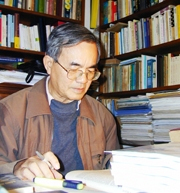
\includegraphics[width= 0.50 \textwidth]{phandinhdieu} 
\end{center}

\textbf{Hiệu Minh Blog}. Giáo sư Phan Đình Diệu làm khoa học, viết nhiều sách, bài báo sắc sảo, và chính luận gây nhiều hiệu ứng xã hội. Ngoài đời, anh còn có những bài thơ hay về những trí thức đáng kính như Tạ Quang Bửu, Trần Đại Nghĩa, Nguyễn Thúc Hào. Có lẽ còn nhiều bài khác, kể cả thơ tình, nhưng chưa công bố, hoặc in rồi nhưng chưa đưa lên mạng.

Có lần anh tâm sự với tôi về Khuất Nguyên (340 TCN – 278 TCN) nổi tiếng của Trung Quốc thời xưa và coi đó là thần tượng “người trong sống trong thời đục”.

Khuất Nguyên có tài học rộng, giỏi về chính trị, có tài văn chương. Nhiều kẻ trong triều ghen ghét, tìm cách hãm hại, ông buồn chán và viết Ly Tao để tả nỗi buồn bị vua bỏ.


Cuối đời, Khuất Nguyên bị vua Tương Vương đày ra phía nam sông Dương Tử. Thất chí,  suốt ngày ca hát như người điên, làm bài phú “Hoài Sa” rồi ông ôm một phiến đá,  trẫm mình xuống sông Mịch La.

Khuất Nguyên có câu nổi tiếng với lão đánh cá khi ông hỏi tại sao đến nỗi phải tự tử “Cả đời đục cả, một mình ta trong; mọi người say cả, một mình ta tỉnh”.

Cảm ơn các còm sỹ Hà Thiên Hậu, Hồ Tú Bảo, Historian, Cao Sơn và nhiều bạn khác đã sưu tầm những bài viết sau đây của Giáo sư Diệu. Nếu ai có những bài khác, xin gửi đến blog để giúp chúng ta hiểu thêm về một Khuất Nguyên khác của thời đại.
\begin{center}
\textbf{Nhớ về một người thầy thanh cao mà bình dị}\\
Tác giả: \textbf{Phan Đình Diệu}

\end{center}
Đầu năm 1953, tôi vào học phổ thông cấp 3 của trường Phan Đình Phùng, tỉnh Hà Tĩnh. Năm học này, trường đã dời địa điểm về xã Ngu Lâm ở phía nam huyên Đức Thọ. Là một học sinh nhà quê từ vùng nông thôn Can Lộc lên học “Trường tỉnh” ở huyên Đức Thọ vào thời đó đối với tôi là một sự kiện lớn, một niềm vinh dự.

Nếu Hà Tĩnh được xem là một tỉnh có truyền thống hiếu học, thì Đức Thọ (cùng với Hương Sơn) là vùng văn hóa tập trung của tỉnh, với biết bao tấm gương về những con người tài năng mà suốt thời tuổi nhỏ tôi vẫn thường được nghe các bậc cha anh nhắc đến với niềm cảm phục, ngưỡng mộ.

Trường Trung học Phan Đình Phùng là trường học lớn nhất tỉnh, nơi có nhiều thầy giáo đã từng dạy học trước Cách mạng tháng Tám, hoặc là các nhà văn, nhà khoa học, nhà hoạt động xã hội, do thời cuộc đưa đẩy đã tụ hội về trường cùng làm cái nghề dạy học vốn được xem là thanh bạch và cao quý. Bọn học trò nhỏ mới được vào trường như chúng tôi trong những buổi đầu nhìn lên các thầy với một niềm tôn kính và ngưỡng mộ, nhưng không khỏi có ít nhiều mặc cảm của sự cách biệt.

Thời gian êm ả trôi qua, và tôi quen dần với cuộc sống chật vật nghèo nàn của một học sinh xa nhà ở trọ và với những buổi học ban đêm đèn dầu không đủ ánh sáng nhưng đầy hấp dẫn bởi những bài giảng nhiệt tình của các thầy mở ra cho chúng tôi niềm đam mê đến với những miền kiến thức mới mẻ về toán học, văn học, địa lý, lịch sử. Những mặc cảm cách biệt qua đi lúc nào không biết, thầy trò, bè bạn dần trở nên gắn bó thân thiết như trong một gia đình.

Tôi nhớ, vào một chiều mùa thu năm 1953, đang ngồi học một mình trong nhà trọ thì chợt nghe tiếng chó sủa, nhìn ra cổng thấy một ông khách cao lớn đội chiếc mũ lá đi vào. Ngỡ ngàng một chút rồi nhận ra ông khách là thầy Trần Quốc Nghệ, tôi vui mừng và lúng túng mời thầy vào nhà như được đón nhận một vinh dự bất ngờ.

Trong mắt tôi và theo những gì mà tôi được biết, thầy Nghệ là một người đa tài, từng trải, một người am hiểu cả Nho học và Tây học, một thầy dạy Văn rất “uyên bác”, còn tôi là học trò binh thường, chưa biểu lộ được một chút đặc sắc gì về môn học của thầy và vẫn nghĩ rằng mình chẳng có gì đáng được thầy để ý. Vậy mà bỗng nhiên được thầy đến chơi.

Nhìn quanh trong nhà thấy không có gì đáng đem ra mời thầy, tôi chỉ vào bếp rót bát nước chè xanh đưa lên bàn rồi ngồi nghe thầy nói. Thầy ân cần hỏi thăm về tình hình sinh hoạt, học hành, khuyến khích phải chăm học, đừng để uổng phí tuổi trẻ.

Trời bỗng nhiên nhiều mây, rồi lất phất mưa bụi. Tôi mừng vì lưu giữ được thầy ở lại lâu hơn, nhưng thật băn khoăn vì tiếp thầy quá ư đạm bạc. Bỗng thầy nhìn ra ngoài vườn rồi bảo tôi: “Cậu ra hái quả khế chua vào đây”.

Trời ơi! Chẳng lẽ tiếp thầy bằng mấy quả khế chua sao? Hái khế xong, tôi đang lúng túng vì không tìm ra được thứ gì có thể ăn với khế (chút đường ngọt cũng không có), thì lại nghe thầy bảo: “Tìm trong nhà có cái bình vôi đưa ra đây”.

Tôi tìm được bình vôi (ăn trầu) đưa ra, thầy điềm nhiên cầm chìa vôi quệt một ít vôi trong bình ra đĩa rồi cắt khế ra từng miếng, chấm vào vôi và đưa lên miệng. “Cậu có biết ăn cách này không?” – Thầy hỏi.

Tôi xúc động nghẹn ngào “Có ạ”, rồi hai thầy trò cùng ngồi nhấm nháp bữa tiệc “khế chấm vôi” và nghe thầy kể bao nhiêu chuyện thú vị về văn hóa sinh hoạt ẩm thực của quê hương.

Cho đến nay đã hơn nửa thế kỷ trôi qua, nhưng kỷ niệm về “bữa tiệc” độc đáo đó vẫn không bao giờ phai mờ trong ký ức tôi, với hình ảnh thân thiết bình dị của thầy và bữa tiệc “khế” như của hai cha con nông dân nghèo trong mái nhà tranh của tuổi thơ quê hương.

Giai đoạn 1953 – 1954 là một giai đoạn nhiều xáo trộn bi thương trên mảnh đất quê hương Nghệ Tĩnh của chúng tôi. Bên cạnh những niềm vui lớn về những chiến thắng của cuộc kháng chiến đang dần đi đến hồi kết, thì những màn đấu tố từ các phong trào “ chống phản động” rồi “giảm tô”, “cải cách ruộng đất” càng ngày càng gay gắt, đưa cả một vùng quê vào cảnh xáo trộn. Thầy giáo và cả các anh chị học sinh lớn tuổi của trường tôi không hiểu vì sao cũng trở thành đối tượng của cuộc đấu tố đó.

Tôi thấy thầy Nghệ vắng mặt ở trường một thời gian. Cho đến một buổi sáng trời mưa phùn vảo khoảng giữa năm 1954, tôi đang đi bộ một mình trên đường từ Lạc Thiện lên thị trấn Đức Thọ thì bổng gặp thầy trong một hoàn cảnh thật trở trêu.

Đường xa mỏi mệt, đang lủi thủi một mình thì thấy từ xa đi theo hướng ngược lại một tốp ba người, người đi giữa dáng cao lớn, mang một chiếc tơi lá, hai người đi kèm sau là hai dân quân, một người cầm súng, một người cầm gậy.

Đi gần thêm một chút, tôi bổng rụng rời nhân ra người đi giữa là thầy Nghệ kính yêu của mình. Tôi không khóc được. Tôi có cảm tưởng thầy cũng nhìn thấy tôi vì thấy thầy chững lại một bước chân. Rồi tất cả lại tiếp tục đi. Tôi hét lên một tiếng “Thầy ơi!” và nghe tiếng quát lại của anh dân quân “Đi đi” và thế là hết. Tôi nhìn vuốt theo bóng thầy đi cao đạo điềm đạm giữa trời mù sương mãi cho đến khi khuất bóng.

Một năm sau, giữa đường phố Tràng Tiền của Hà Nội sau ngày giải phóng, tôi tình cờ lại gặp được thầy. Tôi đã qua cái thời thơ bé và thầy đã có thể nói chuyện với tôi ít nhiều về thời cuộc, về thế thái nhân tình.

Hai thầy trò cùng đi dạo mát một lát, ôn lại những câu chuyện học hành của tôi, còn tôi, vẫn với niềm ngưỡng mộ đối với thầy như xưa, tôi không dám hỏi những chuyện mà tôi e là thầy cũng không muốn trả lời. Đó là vào khoảng thời gian mà báo “Nhân văn” mới bị đình bản, và vụ “Nhân văn, Giai phẩm” đang bắt đầu bị lên án gắt gao, và theo lời đồn đại, thì thầy cũng không phải hoàn toàn bàng quan với những xu hướng đó.

Bẵng đi mấy chục năm, đất nước và quê hương đã đi qua một cuộc chiến tranh khốc liệt, những năm tháng hòa bình nhưng còn đói nghèo vất vả. Cho đến đầu thập niên 1990, tôi mới được gặp thầy. Thầy đã già, nhưng vẫn quắc thước như xưa.

Một lần đến thăm thầy, trước khi ra về, bỗng thầy cầm tay tôi và hỏi: “Nghe nói gần đây cậu có một số bài viết được nhiều người quan tâm, lần sau có đến đưa cho mình xem nhé!”. Tôi vâng dạ, nhưng tiếc là chưa tìm lại được những bài mà thầy yêu cầu thì được biết thầy đã về Hà Tĩnh.

Và với lần về quê đó thầy đã mãi mãi không ra Hà Nội nữa. Theo lời nhắn của thầy qua bạn Nguyễn Quang Thân, tôi có kịp nói chuyện qua điện thoại với thầy một lần, chúc thầy mạnh khỏe để còn hy vọng gặp lại thầy.

Nhưng rồi, thầy đã ra đi. Hôm đến viếng thầy ở nhà cô Lành (Con gái thầy) tôi được xem mấy tấm ảnh về phần mộ của thầy, nơi yên nghỉ của thầy đặt ở lưng chừng núi, nhìn ra một vùng non xanh nước biếc của mây trời Hương Sơn, tôi thầm cầu chúc cho hương hồn của thầy được mãi thanh thản cùng đất trời non nước.

Thầy, một con người thanh cao mà bình dị.



\item Vài kỷ niệm với Giáo sư Phan Đình Diệu \\
\url{http://hieuminh.org/2012/02/02/vai-ky-niem-voi-giao-su-pd-dieu/}

Viện KHVN có hai anh tên vần “iêu”: Viện sỹ Nguyễn Văn Hiệu và Giáo sư Phan Đình Diệu. Một anh là viện trưởng, anh kia là viện phó, cùng giỏi và nổi tiếng khắp thế giới.

Cả hai đã về hưu. Một người huân huy chương đầy ngực, người kia chẳng có cái nào. Nhưng không vì thế mà kém cạnh nhau.


Anh Diệu có con trai là Phan Dương Hiệu. Dân hàn lâm đồn thổi, anh Diệu ghét anh Hiệu, đặt tên con để chửi cho sướng. Thật ra, Dương Hiệu nói ngược là Diệu Hương, tên của anh Diệu và chị vợ là Hương ghép lại, chả liên quan gì đến bác Hiệu.

Ai từng làm việc với anh Hiệu thì phục cũng có mà chê cũng lắm, thậm chí còn gọi đùa là Hiêu, vì hứa mà không làm.

Quân của anh Diệu thì tâm phục, khẩu phục tới 90\%, 10\% còn lại là do tỵ hiềm, ghen ghét, hoặc do lề phải trái. Chưa ai dám gọi anh là Điêu mà dân biết tiếng Pháp gọi anh là Monsieur Dieu – anh Trời.

\begin{center}
\textbf{Nhiệt huyết với khoa học}
\end{center}

Nói về đóng góp của Giáo sư Phan Đình Diệu cho khoa học nước nhà thì báo chí viết chán rồi. Tốt nghiệp tiến sỹ toán lý ở tuổi 30 vào cuối năm 1960 tại Liên Xô, thời đó là ghê răng.

Anh có công lớn trong việc tạo ra ngành Tin học Việt Nam, định hướng phát triển trong nhiều năm. Mình từng nghe các seminar về automat hữu hạn, ngôn ngữ hình thức, lý thuyết mật mã, triết học và toán, hội trường đông nghịt.

Tổng Cua từng viết những chương trình dựa vào thuật toán bảo mật của Giáo sư bằng Pascal vài ngàn lệnh cùng với Vũ Đình Hòa và mấy tay chuyên toán cự phách khác. Anh nói về khóa bảo mật cực phức tạp còn dễ hơn các bạn viết còm. Anh bảo, cái đẹp Toán học nằm ở sự đơn giản và logic. Mình viết blog được là học bài của anh Diệu.

Là người có tâm với khoa học và rất yêu toán và tin, anh bỏ không biết bao công sức để xây dựng ngành này cho nước nhà cùng với những giáo sư đầu ngành như Tạ Quang Bửu, Hoàng  Tụy, Lê Văn Thiêm, Nguyễn Văn Đạo…

Đi sang Pháp, thay vì dành tiền mua xe Peugeot về bán lấy lãi như nhiều người, anh mua rất nhiều linh kiện PC cho Viện. Đến nỗi đám quân thương quá, bảo anh đưa tiền, thay vì mua chip, mấy cha láu cá mua một cái xe gửi cho chị Huơng. Làm khoa học cũng phải có “động cơ”, các lão nói vậy.

Nhớ có lần mưa lụt hầm chứa máy tính ODRA, giáo sư đến thấy thảm cảnh đó mà rơi nước mắt vì biết bao tiền của mới mua được cái máy duy nhất thời đó ở miền Bắc.

Giáo sư nổi tiếng vì những quan điểm chính trị đổi mới vì anh nghiên cứu triết học và toán rất kỹ, hiểu rõ qui luật phát triển. Rất nhiều báo cáo của Đại hội Đảng liên quan đến KHKT thường do anh chấp bút. Tuy vậy, nhiều lời cố vấn quan trọng của người trí thức cũng chỉ dừng trên giá sách.

\begin{center}
\textbf{Những dự đoán tương lai}
\end{center}

Tổng Cua nhớ một số dự đoán tầm quốc gia và cả quốc tế của anh Diệu mà sau đó đã đúng.

Thấy Viện sỹ Nguyễn Văn Hiệu bổ nhiệm cán bộ lung tung, rồi biến viện KH VN thành những công ty nhỏ, Giáo sư đoán, cung cách này sẽ đưa viện khoa học đến sự tàn lụi. Quả thật, “nhân bảo như thần bảo”.

Đọc đề án 112 (tin học hóa quốc gia) năm 2001 có nhiều điểm bất bình thường, anh dự báo, dự án sẽ thất bại và gửi thư khẩn cho Thủ tướng Phan Văn Khải. Quả thật sau 5 năm, ban quản lý ra tòa và hàng nghìn tỷ mất mát.

Có lần đi công tác bên Bulgaria (1986), anh Diệu mang theo cháu Phan Dương Hiệu và bà xã Văn Thị Xuân Hương, em gái của giáo sư Văn Như Cương, toàn vần ương.

Anh kể chuyện năm 1954, tốt nghiệp trung học ở Hà Tĩnh rồi đi bộ ra Hà Nội để học trường ĐH Khoa học. Anh nói là gien của anh là làm toán, không phải để làm quan. Nhưng cuối cùng người ta cứ nhét chức cho anh, khổ thế.

Cuối những năm 1970, cấp trên thấy Giáo sư trẻ và rất giỏi, đề nghị đưa anh vào Đảng để làm cán bộ nguồn, dù khi đó đã làm Viện phó Viện KHVN.

Chị Hương, đảng ủy viên, có trách nhiệm phát triển đảng cho chồng. Tỷ tê về tương lai, rồi lợi ích nếu là người của Đảng thì như thế nào, và khuyên, anh chỉ cần viết đơn là họ kết nạp ngay.

Anh nói, để nghĩ 10 ngày rồi trả lời. Đúng hẹn, anh bảo, Đảng muốn thì cứ kết nạp, cần gì phải viết đơn. Thế là chuyện vào Đảng xếp lại. Quan lộ cũng vì thế mà chẳng hanh thông. Ngang ngạnh kiểu ông đồ xứ Nghệ quả có một không hai.

Nhớ lần đi thang máy lên đỉnh Vitusha của thủ đô Sofia đầy tuyết trắng, thay vì mơ mộng với trời mây, bỗng anh than, với cung cách quản lý của các nước XNCH, thế nào khối này cũng sụp đổ cho mà xem. Lúc đó, Tổng Cua nghe rất choáng, và thấy Giáo sư hơi… phản động.

Anh kể, đã sang Hungaria, CHDC Đức, Ba Lan, Tiệp Khắc, Liên Xô, Mỹ và Tây Âu, nhận xét thế là có lý riêng của mình.

Ba năm sau, bức tường Berlin sụp đổ (1989), kéo theo toàn bộ Đông Âu và Liên Xô tan rã.

Anh là đại biểu Quốc hội lúc hơn 40 tuổi, một trong đại biểu trẻ nhất thời đó. Trong một lần được hỏi về một vị quan cao nhất và ảnh hưởng của ông đối với đất nước, anh Diệu có nói đại ý, vị lãnh đạo ấy rất vĩ đại, đưa cuộc kháng chiến chống Mỹ tới thắng lợi, nhưng vĩ đại hơn, nếu ông từ chức ngay bây giờ.

Lúc đó, vị lãnh đạo kia đang ở thế thượng phong sau 1975 chiến thắng vang dội. Nhưng rồi chính sách tập thể HTX, hợp tỉnh, giá lương tiền quá kém cỏi trong thời bình đã đẩy đất nước đến thảm họa. Người dân chỉ mong ông ấy ra đi.

Mang triết lý chiến tranh vào xây dựng thời bình là không thể, mỗi người có một thời. Anh Diệu từng từ quan về làm nghiên cứu khoa học, góp ý phát triển đất nước theo quan điểm của thời đại mới, cho dù những lời của Giáo sư rất khó nghe đối với nhiều chính trị gia.

Thật tiếc, những đầu óc có tầm vóc quốc tế như Giáo sư Diệu mà ít được sử dụng đúng mục đích. Nước mình quá lãng phí chất xám.

\begin{center}
\textbf{Viện trưởng giỏi việc “nước”, đảm việc nhà}
\end{center}

Viện IOIT có mấy cái nhà ngói hình chữ U. Mỗi lần trời mưa, ếch nhái kêu râm ran. Mình thì tối ngủ bàn cơ quan, ăn cơm tập thể chợ  Ngọc Hà. Gia tài là cái xe đạp Wilga mầu đỏ của Ba Lan, đi vài năm đã hỏng. Quần áo rách dần, tích kê mông, đầu gối, áo sờn. Lốp xe vá chằng vá đụp.

Mặt mũi vêu vao như kẻ chết đói. Đang tuổi ăn tuổi ngủ mà có 13kg gạo/tháng, lương 51 đồng. Mỗi lần về quê, mẹ phải cho thêm vài cân gạo cứu đói vào chiếc ruột tượng, gói cho mấy quả trứng và chai mắm tép. Bố thở dài, kỹ sư chó gì mà nghèo rớt mồng tơi. Hay là về đi cày, ăn no hơn. Học cho lắm chữ mà chẳng nên cơm cháo gì.

Thời đó ai cũng thế. Giáo sư Diệu cũng chẳng hơn gì. Phòng Viện trưởng khoảng $8m^2$, đủ kê cái bàn, 4 cái ghế mây, bàn uống nước, sàn lát gạch thô, trần cót ép, không điều hòa, có cái quạt máy điện cơ chạy lừ đừ như ốm đói.

Nhưng đám trẻ cũng vui vì có em Ngân chân dài, xinh đẹp làm thư ký, đi lại phấp phới. Em Thoa má bánh đúc, trông mỡ màng, làm thư viện. Em Liên cá vàng xinh như mộng, đục lỗ bìa máy tính ODRA.

Các viện sỹ trẻ thi nhau đong đưa, gọi viện là Tán tỉnh và Tiêu khiển cũng không ngoa. Anh cũng thông cảm và bảo, đàn ông thấy người đẹp mà không ngắm thì hoặc anh ta nói dối hoặc là bị bệnh.

Anh Diệu ở tầng 5 bên khu lắp ghép Giảng Võ, vì làm quan được lên tầng cao sạch sẽ và mát. Chỉ tội không có nước. Sáng sáng, trước khi đi làm, Giáo sư cởi trần, xách nước từ tầng một lên tầng năm. Thời đó, ban ngày cả nước lo việc nhà, ban đêm cả nhà lo việc nước, Viện trưởng IOIT cũng vậy thôi.

Khi được cấp nhà rộng hơn ở Đồng Xa, mấy phòng liền, cả gia đình chuyển về đó. Thực không ngờ, nơi đó đồng không mông quạnh, chỉ có đồng lúa, ếch nhái kêu, cào cào châu chấu, thiêu thân và bướm đêm bay rợp trời. Điện mất, nước mất, khổ đủ điều. Viện trưởng tiếp tục thức đêm xếp hàng nước và giặt tã.

Là quân của anh ấy mà Tổng Cua chẳng bao giờ biếu xén thủ trưởng. Trong khi mình sang chơi là chị Hương mời vồn vã, chú ở lại ăn cơm, độc thân trông đói hom hem, khổ thân chú. Thủ trưởng hối lộ quân, chuyện ngược đời.

\begin{center}
\textbf{Nghiên cứu bỏ thuốc lá…ra con trai}
\end{center}

Cái nghề nghiên cứu khoa học nước mình hay lắm. Nghiên cứu một đằng, kết quả ra một nẻo. Giáo sư Diệu nghiên cứu cai thuốc lá thì vợ đẻ con trai.

Chả là Giáo sư có hai cô con gái là Quỳnh Dương và Hà Dương đều rất xinh và hiền. Như nhiều nhà, hình như anh mong có con trai.

\begin{center}
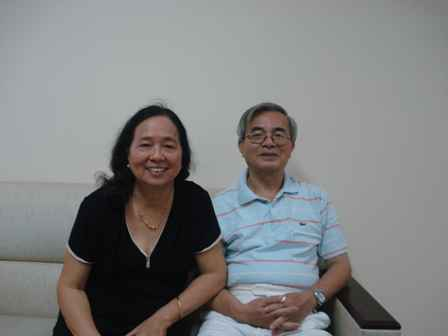
\includegraphics[scale=0.5]{ntngochai_phandinhdieu}\\
 Hai ông bà Hương-Diệu. Ảnh: Ngọc Hải
\end{center}

Anh Diệu nghiện thuốc lá nặng, phòng làm việc lúc nào cũng nghi nghút như cái lò gạch của Nam Cao. Ai đi công tác về cũng biếu thuốc lá, từ 555 đến Pall Mall, Malborro, Tam Đảo, Điện Biên, đủ loại tây ta.

Vợ khuyên bỏ thuốc mãi không được nên ra giá, anh bỏ được, em sẽ đẻ con trai. Giáo sư hứa đại. Thật bất ngờ, cuối năm ấy, cháu trai Phan Dương Hiệu ra đời. Thế là đành phải thực hiện lời hứa. 

Mấy ngày đầu Giáo sư không chịu nổi, cứ cầm điếu thuốc lên, hút vài hơi rồi dụi tắt. Dần dần anh mang các bao thuốc bóc sẵn để khắp nơi trong nhà, trên giá sách, chỗ bàn ăn, văn phòng, nơi hay sờ tới nhất. Nhìn thấy thuốc nhưng không cầm.

Sau ba tuần anh cai hẳn. Vợ đùa dù hơi lo “Anh Diệu bỏ được thuốc nghĩa là anh ấy có thể bỏ vợ được”.

\begin{center}
\textbf{Sửa gáy Giáo sư được trả công bằng…việc làm}
\end{center}
Năm 1977, anh Diệu, lúc đó khoảng 40 tuổi, Viện trưởng Viện Tính toán và Điều khiển đi thăm các nước XHCN và tìm nhân tài cho viện.

Anh tới Ba Lan vào mùa xuân , tuyết vẫn còn dầy. Gần 200 lưu học sinh VN đón giáo sư trẻ ở ký túc xá trên đường $\dot{Z}wirki i Wigury$, đại lộ huyết mạch từ sân bay $Warszawa-Okecie$ về trung tâm Thủ đô Ba Lan.

Bác đoàn trưởng tên là Loan, giám đốc Nha khí tượng Thủy văn đang làm NCS, gõ cửa phòng và bảo “Anh Cua sang nhờ tý”. Mình sang thì gặp Giáo sư Diệu rất trẻ và dễ mến. Anh cười và bảo “Nghe nói cậu biết cắt tóc, chiều nay tớ có cuộc nói chuyện, đi nhiều nước mà không có thời gian. Cậu giúp tớ nhé”.

Giọng Hà Tĩnh hơi nặng, anh xưng cậu cậu tớ tớ, nghe rất thân mật và không hề quan cách. Mới gặp đã thấy rất cảm tình. Trán rộng, mặt sáng, trông rõ là… bác học.

Thời đó sinh viên Ba Lan nổi tiếng tóc dài quần loe, hippi, sexy, thu thập ảnh các cô trần truồng, treo cả lịch 365 thế làm tình trong phòng, chỉ tội không có giáo cụ trực quan để thực hành. Cắt tóc chỉ là xén bớt phần dài dưới gáy.

Trong khi anh Diệu muốn có mái, rẽ ngôi. Loay hoay một hồi, mình cũng sửa xong cái gáy Giáo sư. Anh hỏi Cua “Cậu học nghề chi?”. Mình bảo là Toán Tin. Thế à, cậu về chỗ mình nhé.

Mình bảo, em học dốt lắm, không có bằng đỏ đen gì đâu, lại còn đúp nữa đó. Anh khuyên, tớ không cần bằng đỏ, mà lấy người về nghiên cứu khoa học, và làm được việc. Rồi anh giới thiệu viện, cho số điện thoại, địa chỉ.

Đang du học nên chả nghĩ đến xin việc vì hồi đó cho rằng làm đâu cũng là xây dựng CNXH. Khi về Hà Nội mới hiểu là cái bán kính 3km lấy tâm là bờ Hồ vô cùng quan trọng. Mình lên Nghĩa Đô tìm, không hy vọng anh nhớ mình là ai. Hóa ra Giáo sư nhớ cả tên.

Anh viết thư tay lên Bộ ĐH, thế là mình nghiễm nhiên thành viện sỹ, nằm bàn, cơm tập thể, ước mơ xây XHCN và tiến lên CNCS vào cuối thế kỷ 20.

\begin{center}
\textbf{Khử virus PC được vợ}
\end{center}

Nếu so sánh hai gia đình các anh vần “iệu” ở Viện KH Việt Nam, phải công nhận thuyết “nhân quả” rất đúng. Cha mẹ sống nhân nghĩa để đức cho con. Không biết anh Nguyễn Văn Hiệu thế nào chứ gia đình anh chị Diệu-Hương hạnh phúc, con cái thành đạt.

Con gái thứ là Phan Thị Hà Dương, từng giành được Huy chương Đồng Olympic Toán quốc tế năm 1990, Tiến sỹ Toán khi 26 tuổi và hiện đang công tác trong nước.


\begin{figure}[!ht]
\centering
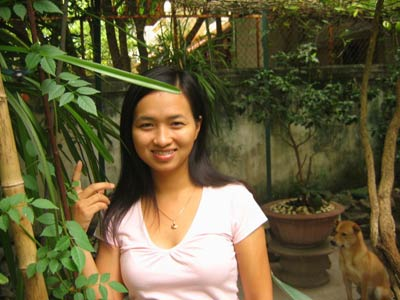
\includegraphics[scale=0.5]{haduong}
\caption{Tiến sỹ toán Hà Dương }
\end{figure}


Cháu Phan Dương Hiệu hồi đi Bulgaria mới 8 tuổi. Lần đi chơi mình bảo, cháu ghi nhật ký thì nên đếm số cột điện treo thang máy từ chân lên đỉnh Vitusha (Sofia) làm kỷ niệm. Có lẽ do gien toán của bố nên cháu thản nhiên, cần gì phải đếm, số cột đã đánh rồi, chỉ cần lên đỉnh và xem số cột cuối là bao nhiêu. Cháu Dương Hiệu hiện là Tiến sỹ Toán đang ở bên Pháp.

Con gái đầu lòng là Quỳnh Dương, đẹp hiền, đảm, ít nói, ngoan, học giỏi và an phận. Hồi ở Đồng Xa, có lần chị Hương nhờ lão Cua tìm thầy trẻ dạy đàn ghi ta cho cháu Quỳnh. Mình hứa lung tung rồi quên tiệt.

Chị Hương quay sang tìm kỹ sư sửa máy tính cho gia đình. Cu Thắng, viện IOIT, khá đẹp trai, có ria mép, thông minh, nhận đến sửa đĩa cứng, rồi cài virus vào, thỉnh thoảng máy lại treo. Mà PC không treo thì Quỳnh Dương cũng gọi anh Thắng đến xem lại cho chắc.

Sau vài tháng, mình hỏi chị Hương là thế nào rồi. Chị bảo chán lắm, tình hình là rất tình hình, lần nào về cũng thấy hai đứa ngồi đối diện nhau, chả thấy nói gì.

Năm ấy Quỳnh Dương sang Pháp du học. Anh chị thở dài, nông nỗi này thì em Quỳnh ế mất. Cả nhà ra sân bay tiễn con, vừa thương vừa nhớ. Cậu Thắng xin đi theo, nhỡ máy laptop của Quỳnh có hỏng gì chăng.

Lên sân bay Nội Bài bịn rịn chia tay. Bỗng anh Diệu thấy con gái cưng, vốn hiền lành, ôm chầm thằng cu chuyên cài virus, nắm tay, nhìn nhau đắm đuối chẳng biết trời đất nào nữa, rồi hôn môi một cái rất dài.

Giáo sư bỏ kính xuống, không thể tin vào mắt mình. Đời anh từng quản lý hàng ngàn cán bộ khoa học, đưa ra những triết lý phát triển cho quốc gia, báo cáo khoa học quốc tế được cả ngàn người thán phục. Rồi suýt bị “dính chưởng” vì chị Dương Thu Hương từng có bài viết đa nguyên của Giáo sư trong vali khi bị bắt ở sân bay. 

Ngay cả cái lý thuyết automat hữu hạn phải gió hay cái máy vi tính đầu tiên của Việt Nam được xuất xưởng, anh cũng không ngạc nhiên bằng nụ hôn giữa thanh thiên bạch nhật của cô con gái  dành cho cu Thắng bên phòng Kỹ thuật số.

Hai vợ chồng choáng váng và chợt hiểu thế nào là virus PC nhiễm sang người. Họ thầm gọi cu Thắng là Thang Dieu – Thằng  Con Trời cho xứng với Monsieur Dieu – Ông Trời Diệu.

Sau cái vụ nhiễm virus ấy, hai đứa có mấy con và hiện đang sống bên Pháp, rất hạnh phúc. Chả hiểu cu Thắng có dạy đàn ghi ta cho Quỳnh không.

Còn Tổng Cua đang làm gì, đố các bạn biết? Lão cố dạy hai thằng cu Hiệu – Minh cách cài virus vào máy tính và học thêm nghề cắt tóc.

HM. 1-2-2012



%\item Interview with the Vietnamese Mathematician Phan Dinh Dieu}
\end{enumerate}



%\section{Bài liệt kê trên Chúng Ta}
%\url{http://www.chungta.com/nhanvat-xahoi/nhan-vat-xa-hoi/phan_dinh_dieu.html}
% \includepdf[pages=1-,noautoscale,pagecommand={\thispagestyle{plain}}]{Docs/2014_ChungTa_PhanDinhDieu.pdf}



\printindex

\bibliographystyle{plain}
{\footnotesize \bibliography{../conf,../abbrev_short,../crypto,../bibfile}}
\bibliography{bodieu}

\end{document}

